\documentclass{article}
\usepackage{amsmath}
\usepackage{color,pxfonts,fix-cm}
\usepackage{latexsym}
\usepackage[mathletters]{ucs}
\DeclareUnicodeCharacter{8211}{\textendash}
\DeclareUnicodeCharacter{177}{$\pm$}
\DeclareUnicodeCharacter{46}{\textperiodcentered}
\DeclareUnicodeCharacter{945}{$\alpha$}
\DeclareUnicodeCharacter{946}{$\beta$}
\DeclareUnicodeCharacter{62}{\textgreater}
\DeclareUnicodeCharacter{8804}{$\leq$}
\DeclareUnicodeCharacter{32}{$\ $}
\usepackage[T1]{fontenc}
\usepackage[utf8x]{inputenc}
\usepackage{pict2e}
\usepackage{wasysym}
\usepackage[english]{babel}
\usepackage{tikz}
\pagestyle{empty}
\usepackage[margin=0in,paperwidth=595pt,paperheight=793pt]{geometry}
\begin{document}
\definecolor{color_283006}{rgb}{1,1,1}
\definecolor{color_29791}{rgb}{0,0,0}
\definecolor{color_241997}{rgb}{0.839216,0.8,0.894118}
\definecolor{color_112230}{rgb}{0.329412,0.2,0.52549}
\definecolor{color_72488}{rgb}{0.168628,0.168628,0.160784}
\definecolor{color_252189}{rgb}{0.905882,0.035294,0.501961}
\begin{tikzpicture}[overlay]\path(0pt,0pt);\end{tikzpicture}
\begin{picture}(-5,0)(2.5,0)
\put(288.9725,-246.4835){\fontsize{44}{1}\usefont{T1}{cmr}{m}{n}\selectfont\color{color_283006} }
\put(180.19,-255.2835){\fontsize{44}{1}\usefont{T1}{cmr}{m}{n}\selectfont\color{color_29791}Soft tissue }
\put(71.42202,-308.0835){\fontsize{44}{1}\usefont{T1}{cmr}{m}{n}\selectfont\color{color_29791}management and bone }
\put(130.074,-360.8835){\fontsize{44}{1}\usefont{T1}{cmr}{m}{n}\selectfont\color{color_29791}augmentation}
\put(487.0161,-255.2835){\fontsize{44}{1}\usefont{T1}{cmr}{m}{n}\selectfont\color{color_283006} }
\put(386.77,-360.8835){\fontsize{44}{1}\usefont{T1}{cmr}{m}{n}\selectfont\color{color_29791}in }
\put(159.422,-413.684){\fontsize{44}{1}\usefont{T1}{cmr}{m}{n}\selectfont\color{color_29791}implantology}
\put(70.9979,-495.6919){\fontsize{30}{1}\usefont{T1}{cmr}{m}{n}\selectfont\color{color_29791}Soft tissue management during}
\put(480.1091,-390.0919){\fontsize{30}{1}\usefont{T1}{cmr}{m}{n}\selectfont\color{color_241997} }
\put(61.3679,-531.6928){\fontsize{30}{1}\usefont{T1}{cmr}{m}{n}\selectfont\color{color_29791}augmentation, implantation, and}
\put(489.7091,-426.0919){\fontsize{30}{1}\usefont{T1}{cmr}{m}{n}\selectfont\color{color_241997} }
\put(139.3379,-567.6928){\fontsize{30}{1}\usefont{T1}{cmr}{m}{n}\selectfont\color{color_29791}second-stage surgery}
\end{picture}
\newpage
\begin{tikzpicture}[overlay]\path(0pt,0pt);\end{tikzpicture}
\begin{picture}(-5,0)(2.5,0)
\put(58.7009,-754.1789){\fontsize{11}{1}\usefont{T1}{cmr}{m}{n}\selectfont\color{color_112230}76}
\put(58.7009,-29.88385){\fontsize{11}{1}\usefont{T1}{cmr}{m}{n}\selectfont\color{color_112230}3}
\put(64.9269,-29.88391){\fontsize{11}{1}\usefont{T1}{cmr}{m}{n}\selectfont\color{color_112230} Soft tissue management and bone augmentation in implantology}
\put(58.7008,-77.22589){\fontsize{14}{1}\usefont{T1}{cmr}{m}{n}\selectfont\color{color_112230}3.1 Introduction}
\put(58.7008,-105.7559){\fontsize{10.8}{1}\usefont{T1}{cmr}{m}{n}\selectfont\color{color_72488}In addition to purely functional rehabilitation, }
\put(58.7008,-120.7571){\fontsize{10.8}{1}\usefont{T1}{cmr}{m}{n}\selectfont\color{color_72488}the esthetic quality of implant treatments is }
\put(58.7008,-135.7583){\fontsize{10.8}{1}\usefont{T1}{cmr}{m}{n}\selectfont\color{color_72488} becoming increasingly important in modern im}
\put(276.2074,-135.7562){\fontsize{10.8}{1}\usefont{T1}{cmr}{m}{n}\selectfont\color{color_72488}-}
\put(58.7008,-150.7563){\fontsize{10.8}{1}\usefont{T1}{cmr}{m}{n}\selectfont\color{color_72488}plantology. Above all, patients consider the }
\put(58.7008,-165.7571){\fontsize{10.8}{1}\usefont{T1}{cmr}{m}{n}\selectfont\color{color_72488} appearance of peri-implant soft tissue and pros}
\put(276.2074,-165.756){\fontsize{10.8}{1}\usefont{T1}{cmr}{m}{n}\selectfont\color{color_72488}-}
\put(58.7008,-180.7561){\fontsize{10.8}{1}\usefont{T1}{cmr}{m}{n}\selectfont\color{color_72488}thetic superstructures to be decisive.}
\put(232.2223,-178.0559){\fontsize{6.48}{1}\usefont{T1}{cmr}{m}{n}\selectfont\color{color_72488}181}
\put(72.8741,-195.7559){\fontsize{10.8}{1}\usefont{T1}{cmr}{m}{n}\selectfont\color{color_72488}The care and preservation of existing soft and }
\put(58.7045,-210.7571){\fontsize{10.8}{1}\usefont{T1}{cmr}{m}{n}\selectfont\color{color_72488}hard tissue is, of course, essential for esthetical}
\put(276.2068,-210.756){\fontsize{10.8}{1}\usefont{T1}{cmr}{m}{n}\selectfont\color{color_72488}-}
\put(58.70016,-225.7562){\fontsize{10.8}{1}\usefont{T1}{cmr}{m}{n}\selectfont\color{color_72488}ly appealing implantology for prosthetic purpos-}
\put(58.70016,-240.7563){\fontsize{10.8}{1}\usefont{T1}{cmr}{m}{n}\selectfont\color{color_72488}es. In many cases where tissue cannot be pre-}
\put(58.70016,-255.7564){\fontsize{10.8}{1}\usefont{T1}{cmr}{m}{n}\selectfont\color{color_72488}served, functional and esthetic results are not }
\put(58.70016,-270.7576){\fontsize{10.8}{1}\usefont{T1}{cmr}{m}{n}\selectfont\color{color_72488}possible without bone augmentation in combi}
\put(276.2068,-270.7565){\fontsize{10.8}{1}\usefont{T1}{cmr}{m}{n}\selectfont\color{color_72488}-}
\put(58.70016,-285.7567){\fontsize{10.8}{1}\usefont{T1}{cmr}{m}{n}\selectfont\color{color_72488}nation with corresponding soft tissue manage-}
\put(58.70016,-300.7568){\fontsize{10.8}{1}\usefont{T1}{cmr}{m}{n}\selectfont\color{color_72488}ment. A preoperative esthetic analysis is recom-}
\put(58.70016,-315.7569){\fontsize{10.8}{1}\usefont{T1}{cmr}{m}{n}\selectfont\color{color_72488}mended in almost all cases to ensure that the }
\put(58.70016,-330.7581){\fontsize{10.8}{1}\usefont{T1}{cmr}{m}{n}\selectfont\color{color_72488}implant is positioned anatomically correctly and }
\put(58.70016,-345.7593){\fontsize{10.8}{1}\usefont{T1}{cmr}{m}{n}\selectfont\color{color_72488}is presented in an optimal manner relative to the }
\put(58.70016,-360.7605){\fontsize{10.8}{1}\usefont{T1}{cmr}{m}{n}\selectfont\color{color_72488}adjacent teeth and soft tissue. Soft tissue man}
\put(276.2068,-360.7572){\fontsize{10.8}{1}\usefont{T1}{cmr}{m}{n}\selectfont\color{color_72488}-}
\put(58.70016,-375.7574){\fontsize{10.8}{1}\usefont{T1}{cmr}{m}{n}\selectfont\color{color_72488}agement is therefore decisive in all surgical in-}
\put(58.70016,-390.7575){\fontsize{10.8}{1}\usefont{T1}{cmr}{m}{n}\selectfont\color{color_72488}terventions for the overall result of augmentative }
\put(58.70016,-405.7587){\fontsize{10.8}{1}\usefont{T1}{cmr}{m}{n}\selectfont\color{color_72488}treatment.}
\put(72.86976,-420.7599){\fontsize{10.8}{1}\usefont{T1}{cmr}{m}{n}\selectfont\color{color_72488}According to Rosenquist,}
\put(194.4442,-418.0559){\fontsize{6.48}{1}\usefont{T1}{cmr}{m}{n}\selectfont\color{color_72488}149}
\put(206.2246,-420.7559){\fontsize{10.8}{1}\usefont{T1}{cmr}{m}{n}\selectfont\color{color_72488} there are four }
\put(58.6966,-435.7571){\fontsize{10.8}{1}\usefont{T1}{cmr}{m}{n}\selectfont\color{color_72488}factors that fundamentally determine the func}
\put(276.2064,-435.756){\fontsize{10.8}{1}\usefont{T1}{cmr}{m}{n}\selectfont\color{color_72488}-}
\put(58.69982,-450.7562){\fontsize{10.8}{1}\usefont{T1}{cmr}{m}{n}\selectfont\color{color_72488}tional and esthetic appearance of soft tissue: 1) }
\put(58.69982,-465.7574){\fontsize{10.8}{1}\usefont{T1}{cmr}{m}{n}\selectfont\color{color_72488}the width and position of the attached kerati}
\put(276.2064,-465.7563){\fontsize{10.8}{1}\usefont{T1}{cmr}{m}{n}\selectfont\color{color_72488}-}
\put(58.69982,-480.7564){\fontsize{10.8}{1}\usefont{T1}{cmr}{m}{n}\selectfont\color{color_72488}nized gingiva; 2) the buccal volume and con-}
\put(58.69982,-495.7565){\fontsize{10.8}{1}\usefont{T1}{cmr}{m}{n}\selectfont\color{color_72488}tour of the alveolar process; 3) the height and }
\put(58.69982,-510.7577){\fontsize{10.8}{1}\usefont{T1}{cmr}{m}{n}\selectfont\color{color_72488}profile of the gingival margin; and 4) the size }
\put(58.69982,-525.7589){\fontsize{10.8}{1}\usefont{T1}{cmr}{m}{n}\selectfont\color{color_72488}and appearance of the interdental and inter}
\put(276.2064,-525.7567){\fontsize{10.8}{1}\usefont{T1}{cmr}{m}{n}\selectfont\color{color_72488}-}
\put(58.69982,-540.7568){\fontsize{10.8}{1}\usefont{T1}{cmr}{m}{n}\selectfont\color{color_72488}implant papillae. However, esthetic results are }
\put(58.69982,-555.7581){\fontsize{10.8}{1}\usefont{T1}{cmr}{m}{n}\selectfont\color{color_72488}often poorly documented in the literature and }
\put(58.69982,-570.7593){\fontsize{10.8}{1}\usefont{T1}{cmr}{m}{n}\selectfont\color{color_72488}are rarely taken into account as a criterion of }
\put(58.69982,-585.7605){\fontsize{10.8}{1}\usefont{T1}{cmr}{m}{n}\selectfont\color{color_72488}treatment success.}
\put(147.2473,-583.0559){\fontsize{6.48}{1}\usefont{T1}{cmr}{m}{n}\selectfont\color{color_72488}16 }
\put(157.4975,-585.7559){\fontsize{10.8}{1}\usefont{T1}{cmr}{m}{n}\selectfont\color{color_72488}Notwithstanding, the ade-}
\put(58.70019,-600.756){\fontsize{10.8}{1}\usefont{T1}{cmr}{m}{n}\selectfont\color{color_72488}quate width of the attached and/or keratinized }
\put(58.70019,-615.7572){\fontsize{10.8}{1}\usefont{T1}{cmr}{m}{n}\selectfont\color{color_72488}mucosa was (and is) regularly discussed in the }
\put(58.70019,-630.7584){\fontsize{10.8}{1}\usefont{T1}{cmr}{m}{n}\selectfont\color{color_72488}clinical literature. A systematic review found }
\put(58.70019,-645.7596){\fontsize{10.8}{1}\usefont{T1}{cmr}{m}{n}\selectfont\color{color_72488}that the amount of plaque accumulation, muco}
\put(276.2068,-645.7564){\fontsize{10.8}{1}\usefont{T1}{cmr}{m}{n}\selectfont\color{color_72488}-}
\put(58.70019,-660.7565){\fontsize{10.8}{1}\usefont{T1}{cmr}{m}{n}\selectfont\color{color_72488}sal inflammation, recessions, and loss of at-}
\put(58.70019,-675.7567){\fontsize{10.8}{1}\usefont{T1}{cmr}{m}{n}\selectfont\color{color_72488}tachment were more expressed to a statistically }
\put(58.70019,-690.7578){\fontsize{10.8}{1}\usefont{T1}{cmr}{m}{n}\selectfont\color{color_72488}significant extent around implants where the }
\put(58.70019,-705.759){\fontsize{10.8}{1}\usefont{T1}{cmr}{m}{n}\selectfont\color{color_72488}width of keratinized mucosa was inade}
\put(276.2068,-705.7569){\fontsize{10.8}{1}\usefont{T1}{cmr}{m}{n}\selectfont\color{color_72488}-}
\put(58.70019,-720.757){\fontsize{10.8}{1}\usefont{T1}{cmr}{m}{n}\selectfont\color{color_72488}quate.}
\put(88.07661,-718.0559){\fontsize{6.48}{1}\usefont{T1}{cmr}{m}{n}\selectfont\color{color_72488}115,147}
\put(113.5815,-720.7559){\fontsize{10.8}{1}\usefont{T1}{cmr}{m}{n}\selectfont\color{color_72488} It has to be noted, however, that }
\put(293.9739,-75.7583){\fontsize{10.8}{1}\usefont{T1}{cmr}{m}{n}\selectfont\color{color_72488}parameters such as bleeding on probing (BoP), }
\put(293.9739,-90.75952){\fontsize{10.8}{1}\usefont{T1}{cmr}{m}{n}\selectfont\color{color_72488}probing depth, and radiographic bone loss may }
\put(293.9739,-105.7607){\fontsize{10.8}{1}\usefont{T1}{cmr}{m}{n}\selectfont\color{color_72488}be worse if the keratinized mucosa is miss}
\put(511.4827,-105.7564){\fontsize{10.8}{1}\usefont{T1}{cmr}{m}{n}\selectfont\color{color_72488}-}
\put(293.9771,-120.7565){\fontsize{10.8}{1}\usefont{T1}{cmr}{m}{n}\selectfont\color{color_72488}ing.}
\put(311.4615,-118.0559){\fontsize{6.48}{1}\usefont{T1}{cmr}{m}{n}\selectfont\color{color_72488}115}
\put(323.2419,-120.7559){\fontsize{10.8}{1}\usefont{T1}{cmr}{m}{n}\selectfont\color{color_72488} In a study by Keeve and Khoury}
\put(481.8677,-118.0559){\fontsize{6.48}{1}\usefont{T1}{cmr}{m}{n}\selectfont\color{color_72488}94}
\put(489.7213,-120.7559){\fontsize{10.8}{1}\usefont{T1}{cmr}{m}{n}\selectfont\color{color_72488} on a }
\put(293.9713,-135.7571){\fontsize{10.8}{1}\usefont{T1}{cmr}{m}{n}\selectfont\color{color_72488}sample of 77 patients with altogether 105 im}
\put(511.4822,-135.756){\fontsize{10.8}{1}\usefont{T1}{cmr}{m}{n}\selectfont\color{color_72488}-}
\put(293.9767,-150.7562){\fontsize{10.8}{1}\usefont{T1}{cmr}{m}{n}\selectfont\color{color_72488}plants over an average observation period of }
\put(293.9767,-165.7574){\fontsize{10.8}{1}\usefont{T1}{cmr}{m}{n}\selectfont\color{color_72488}8 years, a statistically less significant degree of }
\put(293.9767,-180.7586){\fontsize{10.8}{1}\usefont{T1}{cmr}{m}{n}\selectfont\color{color_72488}plaque accumulation, recessions, and mucosal }
\put(293.9767,-195.7598){\fontsize{10.8}{1}\usefont{T1}{cmr}{m}{n}\selectfont\color{color_72488}inflammation around implants with at least }
\put(293.9767,-210.761){\fontsize{10.8}{1}\usefont{T1}{cmr}{m}{n}\selectfont\color{color_72488}2}
\put(300.5212,-210.7607){\fontsize{10.8}{1}\usefont{T1}{cmr}{m}{n}\selectfont\color{color_72488} mm of attached mucosa were observed.}
\put(485.8657,-208.0559){\fontsize{6.48}{1}\usefont{T1}{cmr}{m}{n}\selectfont\color{color_72488}94}
\put(493.7193,-210.7559){\fontsize{10.8}{1}\usefont{T1}{cmr}{m}{n}\selectfont\color{color_72488} Due }
\put(293.9733,-225.7571){\fontsize{10.8}{1}\usefont{T1}{cmr}{m}{n}\selectfont\color{color_72488}to the structural anatomical differences be}
\put(511.4821,-225.756){\fontsize{10.8}{1}\usefont{T1}{cmr}{m}{n}\selectfont\color{color_72488}-}
\put(293.9765,-240.7562){\fontsize{10.8}{1}\usefont{T1}{cmr}{m}{n}\selectfont\color{color_72488}tween teeth and implants, which mostly consist }
\put(293.9765,-255.7574){\fontsize{10.8}{1}\usefont{T1}{cmr}{m}{n}\selectfont\color{color_72488}of missing supracrestal fibers attaching to the }
\put(293.9765,-270.7586){\fontsize{10.8}{1}\usefont{T1}{cmr}{m}{n}\selectfont\color{color_72488}root in the case of titanium or ceramic surfaces, }
\put(293.9765,-285.7598){\fontsize{10.8}{1}\usefont{T1}{cmr}{m}{n}\selectfont\color{color_72488}compromised transmucosal attachment can be }
\put(293.9765,-300.761){\fontsize{10.8}{1}\usefont{T1}{cmr}{m}{n}\selectfont\color{color_72488}expected around implants already after expo}
\put(511.4821,-300.7567){\fontsize{10.8}{1}\usefont{T1}{cmr}{m}{n}\selectfont\color{color_72488}-}
\put(293.9765,-315.7568){\fontsize{10.8}{1}\usefont{T1}{cmr}{m}{n}\selectfont\color{color_72488}sure.}
\put(316.7964,-313.0559){\fontsize{6.48}{1}\usefont{T1}{cmr}{m}{n}\selectfont\color{color_72488}158}
\put(328.5769,-315.7559){\fontsize{10.8}{1}\usefont{T1}{cmr}{m}{n}\selectfont\color{color_72488} The best possible fixation of the muco-}
\put(293.977,-330.756){\fontsize{10.8}{1}\usefont{T1}{cmr}{m}{n}\selectfont\color{color_72488}sa surrounding implants can, at the very least, }
\put(293.977,-345.7572){\fontsize{10.8}{1}\usefont{T1}{cmr}{m}{n}\selectfont\color{color_72488}ensure better daily plaque control and reduce }
\put(293.977,-360.7584){\fontsize{10.8}{1}\usefont{T1}{cmr}{m}{n}\selectfont\color{color_72488}the related inflammatory processes.}
\put(462.9677,-358.0559){\fontsize{6.48}{1}\usefont{T1}{cmr}{m}{n}\selectfont\color{color_72488}178}
\put(474.7482,-360.7559){\fontsize{10.8}{1}\usefont{T1}{cmr}{m}{n}\selectfont\color{color_72488} The ke-}
\put(293.9767,-375.756){\fontsize{10.8}{1}\usefont{T1}{cmr}{m}{n}\selectfont\color{color_72488}ratinization of the tissue in visible areas is in-}
\put(293.9767,-390.7562){\fontsize{10.8}{1}\usefont{T1}{cmr}{m}{n}\selectfont\color{color_72488}dispensable for esthetic reasons (e.g. with a }
\put(293.9767,-405.7574){\fontsize{10.8}{1}\usefont{T1}{cmr}{m}{n}\selectfont\color{color_72488}view to the formation of recessions), and is es}
\put(511.4822,-405.7563){\fontsize{10.8}{1}\usefont{T1}{cmr}{m}{n}\selectfont\color{color_72488}-}
\put(293.9767,-420.7564){\fontsize{10.8}{1}\usefont{T1}{cmr}{m}{n}\selectfont\color{color_72488}sential for the functional and esthetic success }
\put(293.9767,-435.7576){\fontsize{10.8}{1}\usefont{T1}{cmr}{m}{n}\selectfont\color{color_72488}of an implant. It is certainly recommended to }
\put(293.9767,-450.7588){\fontsize{10.8}{1}\usefont{T1}{cmr}{m}{n}\selectfont\color{color_72488}create keratinized, or at least attached, mucosa }
\put(293.9767,-465.76){\fontsize{10.8}{1}\usefont{T1}{cmr}{m}{n}\selectfont\color{color_72488}of an adequate width during implantation or ex}
\put(511.4822,-465.7567){\fontsize{10.8}{1}\usefont{T1}{cmr}{m}{n}\selectfont\color{color_72488}-}
\put(293.9767,-480.7569){\fontsize{10.8}{1}\usefont{T1}{cmr}{m}{n}\selectfont\color{color_72488}posure surgery. }
\put(308.1462,-495.7581){\fontsize{10.8}{1}\usefont{T1}{cmr}{m}{n}\selectfont\color{color_72488}The other important aspect of soft tissue }
\put(293.9767,-510.7593){\fontsize{10.8}{1}\usefont{T1}{cmr}{m}{n}\selectfont\color{color_72488}management is the thickness of the peri-implant }
\put(293.9767,-525.7604){\fontsize{10.8}{1}\usefont{T1}{cmr}{m}{n}\selectfont\color{color_72488}mucosa. Scientific studies have proven that one }
\put(293.9767,-540.7616){\fontsize{10.8}{1}\usefont{T1}{cmr}{m}{n}\selectfont\color{color_72488}should aim for a minimum height of at least }
\put(293.9767,-555.7628){\fontsize{10.8}{1}\usefont{T1}{cmr}{m}{n}\selectfont\color{color_72488}2}
\put(300.4672,-555.7619){\fontsize{10.8}{1}\usefont{T1}{cmr}{m}{n}\selectfont\color{color_72488} mm.}
\put(324.0216,-553.0559){\fontsize{6.48}{1}\usefont{T1}{cmr}{m}{n}\selectfont\color{color_72488}117}
\put(335.7049,-555.7559){\fontsize{10.8}{1}\usefont{T1}{cmr}{m}{n}\selectfont\color{color_72488} A systematic review confirmed that }
\put(293.9737,-570.7571){\fontsize{10.8}{1}\usefont{T1}{cmr}{m}{n}\selectfont\color{color_72488}thicker peri-implant soft tissue layers (> 2 to }
\put(293.9737,-585.7583){\fontsize{10.8}{1}\usefont{T1}{cmr}{m}{n}\selectfont\color{color_72488}3 mm) result in significantly less bone loss }
\put(293.9737,-600.7595){\fontsize{10.8}{1}\usefont{T1}{cmr}{m}{n}\selectfont\color{color_72488}around implants.}
\put(372.0491,-598.0559){\fontsize{6.48}{1}\usefont{T1}{cmr}{m}{n}\selectfont\color{color_72488}171,178}
\put(397.3271,-600.7559){\fontsize{10.8}{1}\usefont{T1}{cmr}{m}{n}\selectfont\color{color_72488} It is therefore reasonable }
\put(293.9711,-615.7571){\fontsize{10.8}{1}\usefont{T1}{cmr}{m}{n}\selectfont\color{color_72488}to prepare not only the width but also the thick}
\put(511.4821,-615.756){\fontsize{10.8}{1}\usefont{T1}{cmr}{m}{n}\selectfont\color{color_72488}-}
\put(293.9765,-630.7562){\fontsize{10.8}{1}\usefont{T1}{cmr}{m}{n}\selectfont\color{color_72488}ness of the attached soft tissue cuff}
\put(457.2184,-630.7559){\fontsize{10.8}{1}\usefont{T1}{cmr}{m}{n}\selectfont\color{color_72488} – particular-}
\put(293.9764,-645.756){\fontsize{10.8}{1}\usefont{T1}{cmr}{m}{n}\selectfont\color{color_72488}ly in esthetic areas – in a manner that enables }
\put(293.9764,-660.7572){\fontsize{10.8}{1}\usefont{T1}{cmr}{m}{n}\selectfont\color{color_72488}optimal long-term success rates.}
\put(308.146,-675.7584){\fontsize{10.8}{1}\usefont{T1}{cmr}{m}{n}\selectfont\color{color_72488}The size and form of the papillae adjacent }
\put(293.9764,-690.7596){\fontsize{10.8}{1}\usefont{T1}{cmr}{m}{n}\selectfont\color{color_72488}to implants are determined by anatomical, sur}
\put(511.4819,-690.7564){\fontsize{10.8}{1}\usefont{T1}{cmr}{m}{n}\selectfont\color{color_72488}-}
\put(293.9764,-705.7565){\fontsize{10.8}{1}\usefont{T1}{cmr}{m}{n}\selectfont\color{color_72488}gical, and restorative factors. To minimize }
\put(293.9764,-720.7577){\fontsize{10.8}{1}\usefont{T1}{cmr}{m}{n}\selectfont\color{color_72488}interimplant bone resorption after prosthetic }
\end{picture}
\newpage
\begin{tikzpicture}[overlay]\path(0pt,0pt);\end{tikzpicture}
\begin{picture}(-5,0)(2.5,0)
\put(493.133,-754.1789){\fontsize{11}{1}\usefont{T1}{cmr}{m}{n}\selectfont\color{color_112230}77}
\put(418.454,-29.88385){\fontsize{11}{1}\usefont{T1}{cmr}{m}{n}\selectfont\color{color_112230}3.1}
\put(435.581,-29.88391){\fontsize{11}{1}\usefont{T1}{cmr}{m}{n}\selectfont\color{color_112230} Introduction}
\put(50.1969,-75.75592){\fontsize{10.8}{1}\usefont{T1}{cmr}{m}{n}\selectfont\color{color_72488}treatment and prevent a significantly greater }
\put(50.1969,-90.75714){\fontsize{10.8}{1}\usefont{T1}{cmr}{m}{n}\selectfont\color{color_72488}degree of bone loss, the distance between two }
\put(50.1969,-105.7584){\fontsize{10.8}{1}\usefont{T1}{cmr}{m}{n}\selectfont\color{color_72488}implants should be no less than 3}
\put(206.1975,-105.7583){\fontsize{10.8}{1}\usefont{T1}{cmr}{m}{n}\selectfont\color{color_72488} mm, and that }
\put(50.19691,-120.7595){\fontsize{10.8}{1}\usefont{T1}{cmr}{m}{n}\selectfont\color{color_72488}between an implant and a natural tooth no less }
\put(50.19691,-135.7607){\fontsize{10.8}{1}\usefont{T1}{cmr}{m}{n}\selectfont\color{color_72488}than 1.5 mm.}
\put(114.6559,-133.0559){\fontsize{6.48}{1}\usefont{T1}{cmr}{m}{n}\selectfont\color{color_72488}65,176}
\put(136.2663,-135.7559){\fontsize{10.8}{1}\usefont{T1}{cmr}{m}{n}\selectfont\color{color_72488} }
\put(64.3707,-150.7571){\fontsize{10.8}{1}\usefont{T1}{cmr}{m}{n}\selectfont\color{color_72488}Interdental papillae are present in 98\% of }
\put(50.2011,-165.7584){\fontsize{10.8}{1}\usefont{T1}{cmr}{m}{n}\selectfont\color{color_72488}cases if the distance between the Limbus alve}
\put(267.7034,-165.7562){\fontsize{10.8}{1}\usefont{T1}{cmr}{m}{n}\selectfont\color{color_72488}-}
\put(50.19785,-180.7563){\fontsize{10.8}{1}\usefont{T1}{cmr}{m}{n}\selectfont\color{color_72488}olaris and the approximal contact point of the }
\put(50.19785,-195.7576){\fontsize{10.8}{1}\usefont{T1}{cmr}{m}{n}\selectfont\color{color_72488}prosthesis is less than 5}
\put(164.2751,-195.7571){\fontsize{10.8}{1}\usefont{T1}{cmr}{m}{n}\selectfont\color{color_72488} mm. If the distance is }
\put(50.19689,-210.7583){\fontsize{10.8}{1}\usefont{T1}{cmr}{m}{n}\selectfont\color{color_72488}increased to 6 to 7 mm, the stability of the }
\put(50.1969,-225.7595){\fontsize{10.8}{1}\usefont{T1}{cmr}{m}{n}\selectfont\color{color_72488}papilla is reduced, and exists in 56\% and 27\% }
\put(50.1969,-240.7607){\fontsize{10.8}{1}\usefont{T1}{cmr}{m}{n}\selectfont\color{color_72488}of cases, respectively.}
\put(151.9638,-238.0559){\fontsize{6.48}{1}\usefont{T1}{cmr}{m}{n}\selectfont\color{color_72488}177}
\put(163.7767,-240.7559){\fontsize{10.8}{1}\usefont{T1}{cmr}{m}{n}\selectfont\color{color_72488} }
\put(64.37349,-255.7571){\fontsize{10.8}{1}\usefont{T1}{cmr}{m}{n}\selectfont\color{color_72488}The formation of papillae between adjacent }
\put(50.20389,-270.7584){\fontsize{10.8}{1}\usefont{T1}{cmr}{m}{n}\selectfont\color{color_72488}implants is more problematic. The size of inter}
\put(267.7029,-270.7562){\fontsize{10.8}{1}\usefont{T1}{cmr}{m}{n}\selectfont\color{color_72488}-}
\put(50.1974,-285.7563){\fontsize{10.8}{1}\usefont{T1}{cmr}{m}{n}\selectfont\color{color_72488}implant papillae can only be predicted up to a }
\put(50.1974,-300.7575){\fontsize{10.8}{1}\usefont{T1}{cmr}{m}{n}\selectfont\color{color_72488}distance of 3}
\put(109.6617,-300.7571){\fontsize{10.8}{1}\usefont{T1}{cmr}{m}{n}\selectfont\color{color_72488} mm between the alveolar bone and }
\put(50.1969,-315.7583){\fontsize{10.8}{1}\usefont{T1}{cmr}{m}{n}\selectfont\color{color_72488}the contact point.}
\put(132.2266,-313.0559){\fontsize{6.48}{1}\usefont{T1}{cmr}{m}{n}\selectfont\color{color_72488}53}
\put(140.0154,-315.7559){\fontsize{10.8}{1}\usefont{T1}{cmr}{m}{n}\selectfont\color{color_72488} A papilla can probably form }
\put(50.1918,-330.7571){\fontsize{10.8}{1}\usefont{T1}{cmr}{m}{n}\selectfont\color{color_72488}between an implant and a tooth at a correspond}
\put(267.7027,-330.756){\fontsize{10.8}{1}\usefont{T1}{cmr}{m}{n}\selectfont\color{color_72488}-}
\put(50.19718,-345.7562){\fontsize{10.8}{1}\usefont{T1}{cmr}{m}{n}\selectfont\color{color_72488}ing vertical distance of 4.5}
\put(175.357,-345.7559){\fontsize{10.8}{1}\usefont{T1}{cmr}{m}{n}\selectfont\color{color_72488} mm.}
\put(198.9112,-343.0559){\fontsize{6.48}{1}\usefont{T1}{cmr}{m}{n}\selectfont\color{color_72488}152,175}
\put(64.3701,-360.7559){\fontsize{10.8}{1}\usefont{T1}{cmr}{m}{n}\selectfont\color{color_72488}In the case of pontic solutions, however, }
\put(50.2005,-375.7571){\fontsize{10.8}{1}\usefont{T1}{cmr}{m}{n}\selectfont\color{color_72488}papilla height is predictable at a distance of }
\put(50.2005,-390.7583){\fontsize{10.8}{1}\usefont{T1}{cmr}{m}{n}\selectfont\color{color_72488}5.5 to 6 mm between the alveolar bone and the }
\put(50.20049,-405.7595){\fontsize{10.8}{1}\usefont{T1}{cmr}{m}{n}\selectfont\color{color_72488}contact point.}
\put(116.279,-403.0559){\fontsize{6.48}{1}\usefont{T1}{cmr}{m}{n}\selectfont\color{color_72488}152}
\put(128.1566,-405.7559){\fontsize{10.8}{1}\usefont{T1}{cmr}{m}{n}\selectfont\color{color_72488} These anatomical indices are }
\put(50.20221,-420.7571){\fontsize{10.8}{1}\usefont{T1}{cmr}{m}{n}\selectfont\color{color_72488}considered indispensable, but they do not }
\put(50.20221,-435.7583){\fontsize{10.8}{1}\usefont{T1}{cmr}{m}{n}\selectfont\color{color_72488}guarantee the formation of a papilla after sur}
\put(267.7034,-435.7561){\fontsize{10.8}{1}\usefont{T1}{cmr}{m}{n}\selectfont\color{color_72488}-}
\put(50.19788,-450.7563){\fontsize{10.8}{1}\usefont{T1}{cmr}{m}{n}\selectfont\color{color_72488}gical procedures.}
\put(130.9209,-448.0559){\fontsize{6.48}{1}\usefont{T1}{cmr}{m}{n}\selectfont\color{color_72488}190}
\put(64.3701,-465.7559){\fontsize{10.8}{1}\usefont{T1}{cmr}{m}{n}\selectfont\color{color_72488}Soft tissue management is a very important }
\put(50.2005,-480.7571){\fontsize{10.8}{1}\usefont{T1}{cmr}{m}{n}\selectfont\color{color_72488}factor in bone augmentation for the following }
\put(50.2005,-495.7583){\fontsize{10.8}{1}\usefont{T1}{cmr}{m}{n}\selectfont\color{color_72488}reasons: 1) for the primary safety of the proced}
\put(267.7028,-495.7561){\fontsize{10.8}{1}\usefont{T1}{cmr}{m}{n}\selectfont\color{color_72488}-}
\put(50.19724,-510.7562){\fontsize{10.8}{1}\usefont{T1}{cmr}{m}{n}\selectfont\color{color_72488}ure; 2) for the esthetic result in the anterior }
\put(50.19724,-525.7574){\fontsize{10.8}{1}\usefont{T1}{cmr}{m}{n}\selectfont\color{color_72488}area, since bony defects are also combined with }
\put(50.19724,-540.7587){\fontsize{10.8}{1}\usefont{T1}{cmr}{m}{n}\selectfont\color{color_72488}poor soft tissue quality; 3) for function, reducing }
\put(50.19724,-555.7598){\fontsize{10.8}{1}\usefont{T1}{cmr}{m}{n}\selectfont\color{color_72488}the muscle activity around the grafted bone and }
\put(50.19724,-570.761){\fontsize{10.8}{1}\usefont{T1}{cmr}{m}{n}\selectfont\color{color_72488}the implants; and 4) for the long-term stability }
\put(50.19724,-585.7622){\fontsize{10.8}{1}\usefont{T1}{cmr}{m}{n}\selectfont\color{color_72488}of the definitive results. Primary, tension-free }
\put(50.19724,-600.7634){\fontsize{10.8}{1}\usefont{T1}{cmr}{m}{n}\selectfont\color{color_72488}wound closure is indispensable in augmentation }
\put(50.19724,-615.7646){\fontsize{10.8}{1}\usefont{T1}{cmr}{m}{n}\selectfont\color{color_72488}measures – bone grafts or guided tissue regen}
\put(267.7028,-615.756){\fontsize{10.8}{1}\usefont{T1}{cmr}{m}{n}\selectfont\color{color_72488}-}
\put(50.19724,-630.7561){\fontsize{10.8}{1}\usefont{T1}{cmr}{m}{n}\selectfont\color{color_72488}eration – and is a decisive prerequisite for the }
\put(50.19724,-645.7573){\fontsize{10.8}{1}\usefont{T1}{cmr}{m}{n}\selectfont\color{color_72488}bacteria-free healing of the graft as well as for }
\put(50.19724,-660.7585){\fontsize{10.8}{1}\usefont{T1}{cmr}{m}{n}\selectfont\color{color_72488}an eventually successful treatment. Gingiva }
\put(50.19724,-675.7598){\fontsize{10.8}{1}\usefont{T1}{cmr}{m}{n}\selectfont\color{color_72488}quantity and quality are important factors, not }
\put(50.19724,-690.7609){\fontsize{10.8}{1}\usefont{T1}{cmr}{m}{n}\selectfont\color{color_72488}only for good primary healing of the grafted bone }
\put(50.19724,-705.7621){\fontsize{10.8}{1}\usefont{T1}{cmr}{m}{n}\selectfont\color{color_72488}to reduce the risk of tissue necrosis and graft }
\put(50.19724,-720.7633){\fontsize{10.8}{1}\usefont{T1}{cmr}{m}{n}\selectfont\color{color_72488}exposure, but also for the long-term stability of }
\put(285.4752,-75.76575){\fontsize{10.8}{1}\usefont{T1}{cmr}{m}{n}\selectfont\color{color_72488}the grafted area. In many cases, it is important }
\put(285.4752,-90.76697){\fontsize{10.8}{1}\usefont{T1}{cmr}{m}{n}\selectfont\color{color_72488}to improve the quality and quantity of the soft }
\put(285.4752,-105.7682){\fontsize{10.8}{1}\usefont{T1}{cmr}{m}{n}\selectfont\color{color_72488}tissue before a bone grafting procedure.}
\put(299.6448,-120.7694){\fontsize{10.8}{1}\usefont{T1}{cmr}{m}{n}\selectfont\color{color_72488}A periosteal incision in line with the Rehr}
\put(502.9786,-120.7565){\fontsize{10.8}{1}\usefont{T1}{cmr}{m}{n}\selectfont\color{color_72488}-}
\put(285.4731,-135.7566){\fontsize{10.8}{1}\usefont{T1}{cmr}{m}{n}\selectfont\color{color_72488}mann technique increases the elasticity of the }
\put(285.4731,-150.7578){\fontsize{10.8}{1}\usefont{T1}{cmr}{m}{n}\selectfont\color{color_72488}flap, so that its edges can be closed with exter}
\put(502.9786,-150.7567){\fontsize{10.8}{1}\usefont{T1}{cmr}{m}{n}\selectfont\color{color_72488}-}
\put(285.4731,-165.7568){\fontsize{10.8}{1}\usefont{T1}{cmr}{m}{n}\selectfont\color{color_72488}nal horizontal mattress sutures or simple inter-}
\put(285.4731,-180.757){\fontsize{10.8}{1}\usefont{T1}{cmr}{m}{n}\selectfont\color{color_72488}rupted sutures without tension in a two-layered }
\put(285.4731,-195.7582){\fontsize{10.8}{1}\usefont{T1}{cmr}{m}{n}\selectfont\color{color_72488}procedure. The disadvantage of this procedure }
\put(285.4731,-210.7594){\fontsize{10.8}{1}\usefont{T1}{cmr}{m}{n}\selectfont\color{color_72488}is the coronal adaptation of the mucogingival }
\put(285.4731,-225.7606){\fontsize{10.8}{1}\usefont{T1}{cmr}{m}{n}\selectfont\color{color_72488}junction during augmentation and implanta}
\put(502.9786,-225.7574){\fontsize{10.8}{1}\usefont{T1}{cmr}{m}{n}\selectfont\color{color_72488}-}
\put(285.4731,-240.7575){\fontsize{10.8}{1}\usefont{T1}{cmr}{m}{n}\selectfont\color{color_72488}tion, which has to be subsequently corrected for }
\put(285.4731,-255.7587){\fontsize{10.8}{1}\usefont{T1}{cmr}{m}{n}\selectfont\color{color_72488}esthetic and functional reasons by a second or }
\put(285.4731,-270.7599){\fontsize{10.8}{1}\usefont{T1}{cmr}{m}{n}\selectfont\color{color_72488}third implant-exposure procedure.}
\put(444.7628,-268.0559){\fontsize{6.48}{1}\usefont{T1}{cmr}{m}{n}\selectfont\color{color_72488}97}
\put(452.6164,-270.7559){\fontsize{10.8}{1}\usefont{T1}{cmr}{m}{n}\selectfont\color{color_72488} Soft tissue }
\put(285.4756,-285.7571){\fontsize{10.8}{1}\usefont{T1}{cmr}{m}{n}\selectfont\color{color_72488}management therefore plays a decisive role in }
\put(285.4756,-300.7583){\fontsize{10.8}{1}\usefont{T1}{cmr}{m}{n}\selectfont\color{color_72488}restoring functional and esthetic soft tissue }
\put(285.4756,-315.7595){\fontsize{10.8}{1}\usefont{T1}{cmr}{m}{n}\selectfont\color{color_72488}harmony.}
\put(285.4725,-357.9331){\fontsize{12.5}{1}\usefont{T1}{cmr}{m}{n}\selectfont\color{color_112230}3.1.1 Anatomy and vascularization of the }
\put(325.16,-372.4331){\fontsize{12.5}{1}\usefont{T1}{cmr}{m}{n}\selectfont\color{color_112230}soft tissue}
\put(285.4725,-390.7559){\fontsize{10.8}{1}\usefont{T1}{cmr}{m}{n}\selectfont\color{color_72488}An understanding of the macro- and micro-ana-}
\put(285.4725,-405.756){\fontsize{10.8}{1}\usefont{T1}{cmr}{m}{n}\selectfont\color{color_72488}tomical structure of periodontal and peri-im-}
\put(285.4725,-420.7562){\fontsize{10.8}{1}\usefont{T1}{cmr}{m}{n}\selectfont\color{color_72488}plant tissue is a prerequisite for understanding }
\put(285.4725,-435.7574){\fontsize{10.8}{1}\usefont{T1}{cmr}{m}{n}\selectfont\color{color_72488}the principles of plastic soft tissue surgery and }
\put(285.4725,-450.7585){\fontsize{10.8}{1}\usefont{T1}{cmr}{m}{n}\selectfont\color{color_72488}exposure techniques. The different anatomical }
\put(285.4725,-465.7597){\fontsize{10.8}{1}\usefont{T1}{cmr}{m}{n}\selectfont\color{color_72488}aspects are briefly presented and explained in }
\put(285.4725,-480.7609){\fontsize{10.8}{1}\usefont{T1}{cmr}{m}{n}\selectfont\color{color_72488}the following sub-sections.}
\put(285.4725,-509.4252){\fontsize{11.5}{1}\usefont{T1}{cmr}{m}{n}\selectfont\color{color_112230}3.1.1.1 Gingiva}
\put(285.4725,-525.7559){\fontsize{10.8}{1}\usefont{T1}{cmr}{m}{n}\selectfont\color{color_72488}The gingiva consists of gingival connective tis-}
\put(285.4725,-540.756){\fontsize{10.8}{1}\usefont{T1}{cmr}{m}{n}\selectfont\color{color_72488}sue and overlying epithelium. With the excep-}
\put(285.4725,-555.7562){\fontsize{10.8}{1}\usefont{T1}{cmr}{m}{n}\selectfont\color{color_72488}tion of interdental cols, its surface is keratinized. }
\put(285.4725,-570.7574){\fontsize{10.8}{1}\usefont{T1}{cmr}{m}{n}\selectfont\color{color_72488}The gingiva is located between the gingival mar}
\put(502.978,-570.7563){\fontsize{10.8}{1}\usefont{T1}{cmr}{m}{n}\selectfont\color{color_72488}-}
\put(285.4725,-585.7564){\fontsize{10.8}{1}\usefont{T1}{cmr}{m}{n}\selectfont\color{color_72488}gin and the mucogingival junction. The thick-}
\put(285.4725,-600.7565){\fontsize{10.8}{1}\usefont{T1}{cmr}{m}{n}\selectfont\color{color_72488}ness of this layer is between 1 and 9}
\put(452.8401,-600.7559){\fontsize{10.8}{1}\usefont{T1}{cmr}{m}{n}\selectfont\color{color_72488} mm,}
\put(476.3685,-598.0559){\fontsize{6.48}{1}\usefont{T1}{cmr}{m}{n}\selectfont\color{color_72488}23}
\put(484.1573,-600.7559){\fontsize{10.8}{1}\usefont{T1}{cmr}{m}{n}\selectfont\color{color_72488} with }
\put(285.4697,-615.7571){\fontsize{10.8}{1}\usefont{T1}{cmr}{m}{n}\selectfont\color{color_72488}an average thickness of about 1 mm.}
\put(471.3469,-613.0559){\fontsize{6.48}{1}\usefont{T1}{cmr}{m}{n}\selectfont\color{color_72488}52}
\put(479.1357,-615.7559){\fontsize{10.8}{1}\usefont{T1}{cmr}{m}{n}\selectfont\color{color_72488} It is }
\put(285.4701,-630.7571){\fontsize{10.8}{1}\usefont{T1}{cmr}{m}{n}\selectfont\color{color_72488}thickest in the maxillary anterior region and }
\put(285.4701,-645.7583){\fontsize{10.8}{1}\usefont{T1}{cmr}{m}{n}\selectfont\color{color_72488}thinnest in the mandibular lingual area.}
\put(479.9772,-643.0559){\fontsize{6.48}{1}\usefont{T1}{cmr}{m}{n}\selectfont\color{color_72488}5}
\put(483.8716,-645.7559){\fontsize{10.8}{1}\usefont{T1}{cmr}{m}{n}\selectfont\color{color_72488} The }
\put(285.4756,-660.7571){\fontsize{10.8}{1}\usefont{T1}{cmr}{m}{n}\selectfont\color{color_72488}width of the gingiva is significantly influenced }
\put(285.4756,-675.7583){\fontsize{10.8}{1}\usefont{T1}{cmr}{m}{n}\selectfont\color{color_72488}by the position of the teeth,}
\put(411.8624,-673.0559){\fontsize{6.48}{1}\usefont{T1}{cmr}{m}{n}\selectfont\color{color_72488}151}
\put(423.5457,-675.7559){\fontsize{10.8}{1}\usefont{T1}{cmr}{m}{n}\selectfont\color{color_72488} and changes with }
\put(285.4677,-690.7571){\fontsize{10.8}{1}\usefont{T1}{cmr}{m}{n}\selectfont\color{color_72488}jaw growth.}
\put(339.0922,-688.0559){\fontsize{6.48}{1}\usefont{T1}{cmr}{m}{n}\selectfont\color{color_72488}9}
\put(342.9866,-690.7559){\fontsize{10.8}{1}\usefont{T1}{cmr}{m}{n}\selectfont\color{color_72488} The orthodontic movement of the }
\put(285.4766,-705.7571){\fontsize{10.8}{1}\usefont{T1}{cmr}{m}{n}\selectfont\color{color_72488}teeth in a bucco-oral direction can therefore cor}
\put(502.9789,-705.756){\fontsize{10.8}{1}\usefont{T1}{cmr}{m}{n}\selectfont\color{color_72488}-}
\put(285.4734,-720.7561){\fontsize{10.8}{1}\usefont{T1}{cmr}{m}{n}\selectfont\color{color_72488}respondingly influence the gingival width.}
\put(478.2833,-718.0559){\fontsize{6.48}{1}\usefont{T1}{cmr}{m}{n}\selectfont\color{color_72488}10}
\end{picture}
\newpage
\begin{tikzpicture}[overlay]\path(0pt,0pt);\end{tikzpicture}
\begin{picture}(-5,0)(2.5,0)
\put(58.7009,-754.1789){\fontsize{11}{1}\usefont{T1}{cmr}{m}{n}\selectfont\color{color_112230}78}
\put(58.7009,-29.88385){\fontsize{11}{1}\usefont{T1}{cmr}{m}{n}\selectfont\color{color_112230}3}
\put(64.9269,-29.88391){\fontsize{11}{1}\usefont{T1}{cmr}{m}{n}\selectfont\color{color_112230} Soft tissue management and bone augmentation in implantology}
\put(72.874,-75.75592){\fontsize{10.8}{1}\usefont{T1}{cmr}{m}{n}\selectfont\color{color_72488}The keratinized, stratified, squamous epi-}
\put(58.70007,-90.75604){\fontsize{10.8}{1}\usefont{T1}{cmr}{m}{n}\selectfont\color{color_72488}thelium reaches up to the cementoenamel }
\put(58.70007,-105.7573){\fontsize{10.8}{1}\usefont{T1}{cmr}{m}{n}\selectfont\color{color_72488}junction and goes over into the sulcus epitheli}
\put(276.2067,-105.7562){\fontsize{10.8}{1}\usefont{T1}{cmr}{m}{n}\selectfont\color{color_72488}-}
\put(58.70007,-120.7563){\fontsize{10.8}{1}\usefont{T1}{cmr}{m}{n}\selectfont\color{color_72488}um to a physiologic depth of about 0.5}
\put(246.2698,-120.7559){\fontsize{10.8}{1}\usefont{T1}{cmr}{m}{n}\selectfont\color{color_72488} mm in }
\put(58.70078,-135.7571){\fontsize{10.8}{1}\usefont{T1}{cmr}{m}{n}\selectfont\color{color_72488}the direction of the periodontal space. The oral }
\put(58.70078,-150.7584){\fontsize{10.8}{1}\usefont{T1}{cmr}{m}{n}\selectfont\color{color_72488}sulcus epithelium is histologically similar to }
\put(58.70078,-165.7596){\fontsize{10.8}{1}\usefont{T1}{cmr}{m}{n}\selectfont\color{color_72488}the gingival epithelium but is less parakerati}
\put(276.2074,-165.7563){\fontsize{10.8}{1}\usefont{T1}{cmr}{m}{n}\selectfont\color{color_72488}-}
\put(58.7008,-180.7565){\fontsize{10.8}{1}\usefont{T1}{cmr}{m}{n}\selectfont\color{color_72488}nized. It is adjoined at the bottom of the sulcus }
\put(58.7008,-195.7577){\fontsize{10.8}{1}\usefont{T1}{cmr}{m}{n}\selectfont\color{color_72488}by the marginal epithelium, with an epithelial }
\put(58.7008,-210.7589){\fontsize{10.8}{1}\usefont{T1}{cmr}{m}{n}\selectfont\color{color_72488}attachment of 1 to 2}
\put(159.7456,-210.7583){\fontsize{10.8}{1}\usefont{T1}{cmr}{m}{n}\selectfont\color{color_72488} mm in width on the sur}
\put(276.2074,-210.7562){\fontsize{10.8}{1}\usefont{T1}{cmr}{m}{n}\selectfont\color{color_72488}-}
\put(58.7008,-225.7563){\fontsize{10.8}{1}\usefont{T1}{cmr}{m}{n}\selectfont\color{color_72488}face of the enamel. The marginal epithelium is }
\put(58.7008,-240.7575){\fontsize{10.8}{1}\usefont{T1}{cmr}{m}{n}\selectfont\color{color_72488}stratified and non-keratinized and has a very }
\put(58.7008,-255.7587){\fontsize{10.8}{1}\usefont{T1}{cmr}{m}{n}\selectfont\color{color_72488}high turnover rate.}
\put(147.1766,-253.0559){\fontsize{6.48}{1}\usefont{T1}{cmr}{m}{n}\selectfont\color{color_72488}156}
\put(159.0542,-255.7559){\fontsize{10.8}{1}\usefont{T1}{cmr}{m}{n}\selectfont\color{color_72488} It is completely regener-}
\put(58.70061,-270.756){\fontsize{10.8}{1}\usefont{T1}{cmr}{m}{n}\selectfont\color{color_72488}ated every 4 to 6 days by proliferating cell lay-}
\put(58.70061,-285.7562){\fontsize{10.8}{1}\usefont{T1}{cmr}{m}{n}\selectfont\color{color_72488}ers. If the marginal epithelia of adjacent teeth }
\put(58.70061,-300.7574){\fontsize{10.8}{1}\usefont{T1}{cmr}{m}{n}\selectfont\color{color_72488}or implants adjoin, a non-keratinized col of a }
\put(58.70061,-315.7585){\fontsize{10.8}{1}\usefont{T1}{cmr}{m}{n}\selectfont\color{color_72488}papilla is formed.}
\put(141.7658,-313.0559){\fontsize{6.48}{1}\usefont{T1}{cmr}{m}{n}\selectfont\color{color_72488}81}
\put(149.6842,-315.7559){\fontsize{10.8}{1}\usefont{T1}{cmr}{m}{n}\selectfont\color{color_72488} This takes on a saddle-like }
\put(58.70499,-330.7571){\fontsize{10.8}{1}\usefont{T1}{cmr}{m}{n}\selectfont\color{color_72488}shape in the interdental area and is dependent }
\put(58.70499,-345.7583){\fontsize{10.8}{1}\usefont{T1}{cmr}{m}{n}\selectfont\color{color_72488}on the shape and dimensions of the approximal }
\put(58.70499,-360.7595){\fontsize{10.8}{1}\usefont{T1}{cmr}{m}{n}\selectfont\color{color_72488}contact point. The function of the marginal ep}
\put(276.2073,-360.7563){\fontsize{10.8}{1}\usefont{T1}{cmr}{m}{n}\selectfont\color{color_72488}-}
\put(58.70068,-375.7564){\fontsize{10.8}{1}\usefont{T1}{cmr}{m}{n}\selectfont\color{color_72488}ithelium is to protect the underlying bone from }
\put(58.70068,-390.7576){\fontsize{10.8}{1}\usefont{T1}{cmr}{m}{n}\selectfont\color{color_72488}penetrating micro-organisms. This contact and }
\put(58.70068,-405.7588){\fontsize{10.8}{1}\usefont{T1}{cmr}{m}{n}\selectfont\color{color_72488}reaction zone ensures that the organism per}
\put(276.2073,-405.7566){\fontsize{10.8}{1}\usefont{T1}{cmr}{m}{n}\selectfont\color{color_72488}-}
\put(58.70068,-420.7567){\fontsize{10.8}{1}\usefont{T1}{cmr}{m}{n}\selectfont\color{color_72488}forms immunologic engagement with chemo-}
\put(58.70068,-435.7568){\fontsize{10.8}{1}\usefont{T1}{cmr}{m}{n}\selectfont\color{color_72488}taxis and humoral defense away from the }
\put(58.70068,-450.758){\fontsize{10.8}{1}\usefont{T1}{cmr}{m}{n}\selectfont\color{color_72488}bones. }
\put(72.87028,-465.7592){\fontsize{10.8}{1}\usefont{T1}{cmr}{m}{n}\selectfont\color{color_72488}This attached gingiva reaching up to the }
\put(58.70068,-480.7604){\fontsize{10.8}{1}\usefont{T1}{cmr}{m}{n}\selectfont\color{color_72488}mucogingival junction does not shift relative to }
\put(58.70068,-495.7616){\fontsize{10.8}{1}\usefont{T1}{cmr}{m}{n}\selectfont\color{color_72488}the alveolar process, and the connective tissue }
\put(58.70068,-510.7628){\fontsize{10.8}{1}\usefont{T1}{cmr}{m}{n}\selectfont\color{color_72488}matrix consists of collagen fibers to about 60\%. }
\put(58.70068,-525.764){\fontsize{10.8}{1}\usefont{T1}{cmr}{m}{n}\selectfont\color{color_72488}It forms the supra-alveolar and supracrestal fi}
\put(276.2073,-525.7564){\fontsize{10.8}{1}\usefont{T1}{cmr}{m}{n}\selectfont\color{color_72488}-}
\put(58.70068,-540.7565){\fontsize{10.8}{1}\usefont{T1}{cmr}{m}{n}\selectfont\color{color_72488}ber apparatus of the tooth or implant. The col-}
\put(58.70068,-555.7567){\fontsize{10.8}{1}\usefont{T1}{cmr}{m}{n}\selectfont\color{color_72488}lagen fibers are attached to the teeth in }
\put(58.70068,-570.7579){\fontsize{10.8}{1}\usefont{T1}{cmr}{m}{n}\selectfont\color{color_72488}three-dimensional (3D) structures. They have a }
\put(58.70068,-585.759){\fontsize{10.8}{1}\usefont{T1}{cmr}{m}{n}\selectfont\color{color_72488}stabilizing function as regards the position of }
\put(58.70068,-600.7603){\fontsize{10.8}{1}\usefont{T1}{cmr}{m}{n}\selectfont\color{color_72488}the teeth, and act as a functional unit of the }
\put(58.70068,-615.7615){\fontsize{10.8}{1}\usefont{T1}{cmr}{m}{n}\selectfont\color{color_72488}periodontium in the root cementum and the al}
\put(276.2073,-615.7571){\fontsize{10.8}{1}\usefont{T1}{cmr}{m}{n}\selectfont\color{color_72488}-}
\put(58.70068,-630.7573){\fontsize{10.8}{1}\usefont{T1}{cmr}{m}{n}\selectfont\color{color_72488}veolar bone.}
\put(116.0213,-628.0559){\fontsize{6.48}{1}\usefont{T1}{cmr}{m}{n}\selectfont\color{color_72488}66}
\put(123.9398,-630.7559){\fontsize{10.8}{1}\usefont{T1}{cmr}{m}{n}\selectfont\color{color_72488} }
\put(72.8774,-645.7571){\fontsize{10.8}{1}\usefont{T1}{cmr}{m}{n}\selectfont\color{color_72488}The keratinization of the gingival epithelium }
\put(58.70779,-660.7583){\fontsize{10.8}{1}\usefont{T1}{cmr}{m}{n}\selectfont\color{color_72488}does not result from functional wear but is rath}
\put(276.2068,-660.7562){\fontsize{10.8}{1}\usefont{T1}{cmr}{m}{n}\selectfont\color{color_72488}-}
\put(58.70022,-675.7563){\fontsize{10.8}{1}\usefont{T1}{cmr}{m}{n}\selectfont\color{color_72488}er determined by genetic factors in the underly-}
\put(58.70022,-690.7564){\fontsize{10.8}{1}\usefont{T1}{cmr}{m}{n}\selectfont\color{color_72488}ing connective tissue.}
\put(160.4574,-688.0559){\fontsize{6.48}{1}\usefont{T1}{cmr}{m}{n}\selectfont\color{color_72488}91,92}
\put(293.9764,-74.4209){\fontsize{11.5}{1}\usefont{T1}{cmr}{m}{n}\selectfont\color{color_112230}3.1.1.2 Peri-implant mucosa}
\put(293.9764,-90.75592){\fontsize{10.8}{1}\usefont{T1}{cmr}{m}{n}\selectfont\color{color_72488}The size, shape, and anatomy of the peri-im-}
\put(293.9764,-105.756){\fontsize{10.8}{1}\usefont{T1}{cmr}{m}{n}\selectfont\color{color_72488}plant soft tissue depends on wound healing de-}
\put(293.9764,-120.7562){\fontsize{10.8}{1}\usefont{T1}{cmr}{m}{n}\selectfont\color{color_72488}termined by the position of the implant and by }
\put(293.9764,-135.7574){\fontsize{10.8}{1}\usefont{T1}{cmr}{m}{n}\selectfont\color{color_72488}the implant system and exposure techniques }
\put(293.9764,-150.7586){\fontsize{10.8}{1}\usefont{T1}{cmr}{m}{n}\selectfont\color{color_72488}used. It is comparable to the clinical character}
\put(511.4819,-150.7565){\fontsize{10.8}{1}\usefont{T1}{cmr}{m}{n}\selectfont\color{color_72488}-}
\put(293.9764,-165.7566){\fontsize{10.8}{1}\usefont{T1}{cmr}{m}{n}\selectfont\color{color_72488}istics of soft tissue around natural teeth.}
\put(479.744,-163.0558){\fontsize{6.48}{1}\usefont{T1}{cmr}{m}{n}\selectfont\color{color_72488}18,112,155}
\put(308.1496,-180.7559){\fontsize{10.8}{1}\usefont{T1}{cmr}{m}{n}\selectfont\color{color_72488}It has to be taken into account that instead of }
\put(293.98,-195.7571){\fontsize{10.8}{1}\usefont{T1}{cmr}{m}{n}\selectfont\color{color_72488}a periodontal ligament with physiologic mobility }
\put(293.98,-210.7584){\fontsize{10.8}{1}\usefont{T1}{cmr}{m}{n}\selectfont\color{color_72488}in relation to the anchorage, the implant has an }
\put(293.98,-225.7596){\fontsize{10.8}{1}\usefont{T1}{cmr}{m}{n}\selectfont\color{color_72488}osseointegrative connection with the alveolar }
\put(293.98,-240.7608){\fontsize{10.8}{1}\usefont{T1}{cmr}{m}{n}\selectfont\color{color_72488}bone. As a result, the peri-implant connective tis}
\put(511.4823,-240.7565){\fontsize{10.8}{1}\usefont{T1}{cmr}{m}{n}\selectfont\color{color_72488}-}
\put(293.9768,-255.7566){\fontsize{10.8}{1}\usefont{T1}{cmr}{m}{n}\selectfont\color{color_72488}sue fibers around the abutment or the surface of }
\put(293.9768,-270.7578){\fontsize{10.8}{1}\usefont{T1}{cmr}{m}{n}\selectfont\color{color_72488}the implant are arranged in a parallel position in }
\put(293.9768,-285.759){\fontsize{10.8}{1}\usefont{T1}{cmr}{m}{n}\selectfont\color{color_72488}the supracrestal area, as opposed to being an}
\put(511.4823,-285.7569){\fontsize{10.8}{1}\usefont{T1}{cmr}{m}{n}\selectfont\color{color_72488}-}
\put(293.9768,-300.757){\fontsize{10.8}{1}\usefont{T1}{cmr}{m}{n}\selectfont\color{color_72488}chored to the dental root cementum.}
\put(486.4312,-298.0558){\fontsize{6.48}{1}\usefont{T1}{cmr}{m}{n}\selectfont\color{color_72488}1,2,17,18}
\put(515.0787,-300.7559){\fontsize{10.8}{1}\usefont{T1}{cmr}{m}{n}\selectfont\color{color_72488} }
\put(293.9811,-315.7571){\fontsize{10.8}{1}\usefont{T1}{cmr}{m}{n}\selectfont\color{color_72488}Peri-implant connective tissue also has a higher }
\put(293.9811,-330.7583){\fontsize{10.8}{1}\usefont{T1}{cmr}{m}{n}\selectfont\color{color_72488}ratio of collagen fibers and a lower ratio of fibro}
\put(511.4823,-330.7561){\fontsize{10.8}{1}\usefont{T1}{cmr}{m}{n}\selectfont\color{color_72488}-}
\put(293.9768,-345.7563){\fontsize{10.8}{1}\usefont{T1}{cmr}{m}{n}\selectfont\color{color_72488}blasts, and as such is very similar to scar tissue }
\put(293.9768,-360.7574){\fontsize{10.8}{1}\usefont{T1}{cmr}{m}{n}\selectfont\color{color_72488}in histomorphologic terms.}
\put(414.6975,-358.0558){\fontsize{6.48}{1}\usefont{T1}{cmr}{m}{n}\selectfont\color{color_72488}124,157}
\put(308.1496,-375.7558){\fontsize{10.8}{1}\usefont{T1}{cmr}{m}{n}\selectfont\color{color_72488}While the vascular supply of the gingiva is se-}
\put(293.9768,-390.7559){\fontsize{10.8}{1}\usefont{T1}{cmr}{m}{n}\selectfont\color{color_72488}cured from the three anastomosing areas of the }
\put(293.9768,-405.7571){\fontsize{10.8}{1}\usefont{T1}{cmr}{m}{n}\selectfont\color{color_72488}interdental septa, the periodontal ligament, and }
\put(293.9768,-420.7583){\fontsize{10.8}{1}\usefont{T1}{cmr}{m}{n}\selectfont\color{color_72488}the oral mucosa, peri-implant connective tissue }
\put(293.9768,-435.7595){\fontsize{10.8}{1}\usefont{T1}{cmr}{m}{n}\selectfont\color{color_72488}shows a relatively low level of vascularization. As }
\put(293.9768,-450.7607){\fontsize{10.8}{1}\usefont{T1}{cmr}{m}{n}\selectfont\color{color_72488}a result of osseointegration, the vessels from the }
\put(293.9768,-465.7619){\fontsize{10.8}{1}\usefont{T1}{cmr}{m}{n}\selectfont\color{color_72488}periodontal ligament no longer exist, which means }
\put(293.9768,-480.7631){\fontsize{10.8}{1}\usefont{T1}{cmr}{m}{n}\selectfont\color{color_72488}that the vascular supply of the peri-implant mu}
\put(511.4823,-480.7555){\fontsize{10.8}{1}\usefont{T1}{cmr}{m}{n}\selectfont\color{color_72488}-}
\put(293.9768,-495.7556){\fontsize{10.8}{1}\usefont{T1}{cmr}{m}{n}\selectfont\color{color_72488}cosa is almost exclusively ensured through su-}
\put(293.9768,-510.7557){\fontsize{10.8}{1}\usefont{T1}{cmr}{m}{n}\selectfont\color{color_72488}praperiosteal vessels and a small number of ves-}
\put(293.9768,-525.7559){\fontsize{10.8}{1}\usefont{T1}{cmr}{m}{n}\selectfont\color{color_72488}sels emerging from the bone.}
\put(436.6224,-523.0558){\fontsize{6.48}{1}\usefont{T1}{cmr}{m}{n}\selectfont\color{color_72488}19}
\put(444.2687,-525.7558){\fontsize{10.8}{1}\usefont{T1}{cmr}{m}{n}\selectfont\color{color_72488} External bone }
\put(293.9759,-540.757){\fontsize{10.8}{1}\usefont{T1}{cmr}{m}{n}\selectfont\color{color_72488}surfaces are covered by a thin, inelastic layer of }
\put(293.9759,-555.7582){\fontsize{10.8}{1}\usefont{T1}{cmr}{m}{n}\selectfont\color{color_72488}connective tissue that is rich in collagen – the }
\put(293.9759,-570.7594){\fontsize{10.8}{1}\usefont{T1}{cmr}{m}{n}\selectfont\color{color_72488}so-called ‘periosteum.’ In addition to osteoblasts, }
\put(293.9759,-585.7606){\fontsize{10.8}{1}\usefont{T1}{cmr}{m}{n}\selectfont\color{color_72488}osteoclasts, and the corresponding precursor }
\put(293.9759,-600.7618){\fontsize{10.8}{1}\usefont{T1}{cmr}{m}{n}\selectfont\color{color_72488}cells, the periosteum also contains a large num}
\put(511.4825,-600.7564){\fontsize{10.8}{1}\usefont{T1}{cmr}{m}{n}\selectfont\color{color_72488}-}
\put(293.977,-615.7565){\fontsize{10.8}{1}\usefont{T1}{cmr}{m}{n}\selectfont\color{color_72488}ber of blood vessels and nerves, which are of par-}
\put(293.977,-630.7567){\fontsize{10.8}{1}\usefont{T1}{cmr}{m}{n}\selectfont\color{color_72488}ticular significance for the regeneration of the }
\put(293.977,-645.7578){\fontsize{10.8}{1}\usefont{T1}{cmr}{m}{n}\selectfont\color{color_72488}freshly augmented bone, and may only be sepa}
\put(511.4825,-645.7568){\fontsize{10.8}{1}\usefont{T1}{cmr}{m}{n}\selectfont\color{color_72488}-}
\put(293.977,-660.7569){\fontsize{10.8}{1}\usefont{T1}{cmr}{m}{n}\selectfont\color{color_72488}rated during exposure measures above the im-}
\put(293.977,-675.757){\fontsize{10.8}{1}\usefont{T1}{cmr}{m}{n}\selectfont\color{color_72488}plant cover screws with the greatest possible care }
\put(293.977,-690.7582){\fontsize{10.8}{1}\usefont{T1}{cmr}{m}{n}\selectfont\color{color_72488}as regards the insertion of the gingiva former.}
\put(308.1465,-705.7594){\fontsize{10.8}{1}\usefont{T1}{cmr}{m}{n}\selectfont\color{color_72488}In particular, during surgical soft tissue man}
\put(511.4825,-705.7572){\fontsize{10.8}{1}\usefont{T1}{cmr}{m}{n}\selectfont\color{color_72488}-}
\put(293.977,-720.7573){\fontsize{10.8}{1}\usefont{T1}{cmr}{m}{n}\selectfont\color{color_72488}agement around implants, the scarred histo}
\put(511.4873,-720.7559){\fontsize{10.8}{1}\usefont{T1}{cmr}{m}{n}\selectfont\color{color_72488}-}
\end{picture}
\newpage
\begin{tikzpicture}[overlay]\path(0pt,0pt);\end{tikzpicture}
\begin{picture}(-5,0)(2.5,0)
\put(493.133,-754.1789){\fontsize{11}{1}\usefont{T1}{cmr}{m}{n}\selectfont\color{color_112230}79}
\put(418.454,-29.88385){\fontsize{11}{1}\usefont{T1}{cmr}{m}{n}\selectfont\color{color_112230}3.1}
\put(435.581,-29.88391){\fontsize{11}{1}\usefont{T1}{cmr}{m}{n}\selectfont\color{color_112230} Introduction}
\put(50.1969,-75.75592){\fontsize{10.8}{1}\usefont{T1}{cmr}{m}{n}\selectfont\color{color_72488}morphometry of the implant, the lack of an-}
\put(50.19691,-90.75604){\fontsize{10.8}{1}\usefont{T1}{cmr}{m}{n}\selectfont\color{color_72488}chored fibers, and the comparatively poor }
\put(50.19691,-105.7573){\fontsize{10.8}{1}\usefont{T1}{cmr}{m}{n}\selectfont\color{color_72488}vascularization of peri-implant mucosa should }
\put(50.19691,-120.7585){\fontsize{10.8}{1}\usefont{T1}{cmr}{m}{n}\selectfont\color{color_72488}in consequence be taken into account. Based on }
\put(50.19691,-135.7597){\fontsize{10.8}{1}\usefont{T1}{cmr}{m}{n}\selectfont\color{color_72488}these differences, a reduced resistance to me}
\put(267.7024,-135.7565){\fontsize{10.8}{1}\usefont{T1}{cmr}{m}{n}\selectfont\color{color_72488}-}
\put(50.19691,-150.7566){\fontsize{10.8}{1}\usefont{T1}{cmr}{m}{n}\selectfont\color{color_72488}chanical and microbiologic impacts as well as a }
\put(50.19691,-165.7578){\fontsize{10.8}{1}\usefont{T1}{cmr}{m}{n}\selectfont\color{color_72488}compromised healing potential after surgical in}
\put(267.7024,-165.7567){\fontsize{10.8}{1}\usefont{T1}{cmr}{m}{n}\selectfont\color{color_72488}-}
\put(50.19691,-180.7568){\fontsize{10.8}{1}\usefont{T1}{cmr}{m}{n}\selectfont\color{color_72488}terventions can be expected due to the poorer }
\put(50.19691,-195.7581){\fontsize{10.8}{1}\usefont{T1}{cmr}{m}{n}\selectfont\color{color_72488}vascular supply.}
\put(123.5874,-193.0559){\fontsize{6.48}{1}\usefont{T1}{cmr}{m}{n}\selectfont\color{color_72488}116}
\put(50.1969,-224.4252){\fontsize{11.5}{1}\usefont{T1}{cmr}{m}{n}\selectfont\color{color_112230}3.1.1.3 Biologic width}
\put(50.1969,-240.7559){\fontsize{10.8}{1}\usefont{T1}{cmr}{m}{n}\selectfont\color{color_72488}The special structure of the gingival tissue around }
\put(50.1969,-255.7571){\fontsize{10.8}{1}\usefont{T1}{cmr}{m}{n}\selectfont\color{color_72488}teeth and implants is a unique anatomical situa}
\put(267.7024,-255.756){\fontsize{10.8}{1}\usefont{T1}{cmr}{m}{n}\selectfont\color{color_72488}-}
\put(50.19691,-270.7562){\fontsize{10.8}{1}\usefont{T1}{cmr}{m}{n}\selectfont\color{color_72488}tion, where epithelial integrity is in}
\put(205.0257,-270.7559){\fontsize{10.8}{1}\usefont{T1}{cmr}{m}{n}\selectfont\color{color_72488} terrupted. This }
\put(50.19689,-285.7571){\fontsize{10.8}{1}\usefont{T1}{cmr}{m}{n}\selectfont\color{color_72488}involves the formation of a combination of epithe}
\put(267.7024,-285.756){\fontsize{10.8}{1}\usefont{T1}{cmr}{m}{n}\selectfont\color{color_72488}-}
\put(50.19688,-300.7562){\fontsize{10.8}{1}\usefont{T1}{cmr}{m}{n}\selectfont\color{color_72488}lial attachment against microbiological impacts }
\put(50.19688,-315.7574){\fontsize{10.8}{1}\usefont{T1}{cmr}{m}{n}\selectfont\color{color_72488}and a connective tissue attachment against me}
\put(267.7024,-315.7563){\fontsize{10.8}{1}\usefont{T1}{cmr}{m}{n}\selectfont\color{color_72488}-}
\put(50.19688,-330.7564){\fontsize{10.8}{1}\usefont{T1}{cmr}{m}{n}\selectfont\color{color_72488}chanical impacts, which is referred to as biologic }
\put(50.19688,-345.7576){\fontsize{10.8}{1}\usefont{T1}{cmr}{m}{n}\selectfont\color{color_72488}width.}
\put(78.0066,-343.0559){\fontsize{6.48}{1}\usefont{T1}{cmr}{m}{n}\selectfont\color{color_72488}84}
\put(85.7954,-345.7559){\fontsize{10.8}{1}\usefont{T1}{cmr}{m}{n}\selectfont\color{color_72488} }
\put(64.3682,-360.7571){\fontsize{10.8}{1}\usefont{T1}{cmr}{m}{n}\selectfont\color{color_72488}Around teeth, the biologic width has a verti}
\put(267.703,-360.756){\fontsize{10.8}{1}\usefont{T1}{cmr}{m}{n}\selectfont\color{color_72488}-}
\put(50.19752,-375.7562){\fontsize{10.8}{1}\usefont{T1}{cmr}{m}{n}\selectfont\color{color_72488}cal dimension of 2.04}
\put(152.6997,-375.7559){\fontsize{10.8}{1}\usefont{T1}{cmr}{m}{n}\selectfont\color{color_72488} mm, of which an average }
\put(50.19689,-390.7571){\fontsize{10.8}{1}\usefont{T1}{cmr}{m}{n}\selectfont\color{color_72488}of 1.07 mm consists of connective tissue at}
\put(267.7024,-390.756){\fontsize{10.8}{1}\usefont{T1}{cmr}{m}{n}\selectfont\color{color_72488}-}
\put(50.19688,-405.7562){\fontsize{10.8}{1}\usefont{T1}{cmr}{m}{n}\selectfont\color{color_72488}tachment and 0.97}
\put(146.9109,-405.7559){\fontsize{10.8}{1}\usefont{T1}{cmr}{m}{n}\selectfont\color{color_72488} mm of epithelial attach-}
\put(50.19691,-420.756){\fontsize{10.8}{1}\usefont{T1}{cmr}{m}{n}\selectfont\color{color_72488}ment.}
\put(76.9482,-418.0559){\fontsize{6.48}{1}\usefont{T1}{cmr}{m}{n}\selectfont\color{color_72488}66}
\put(84.73701,-420.7559){\fontsize{10.8}{1}\usefont{T1}{cmr}{m}{n}\selectfont\color{color_72488} Following exposure, a biologic width }
\put(50.19861,-435.7571){\fontsize{10.8}{1}\usefont{T1}{cmr}{m}{n}\selectfont\color{color_72488}also forms around implants. The connective tis}
\put(267.703,-435.756){\fontsize{10.8}{1}\usefont{T1}{cmr}{m}{n}\selectfont\color{color_72488}-}
\put(50.19752,-450.7562){\fontsize{10.8}{1}\usefont{T1}{cmr}{m}{n}\selectfont\color{color_72488}sue attachment around implants is very constant }
\put(50.19752,-465.7574){\fontsize{10.8}{1}\usefont{T1}{cmr}{m}{n}\selectfont\color{color_72488}compared with that of teeth, and has a width of }
\put(50.19752,-480.7585){\fontsize{10.8}{1}\usefont{T1}{cmr}{m}{n}\selectfont\color{color_72488}about 1}
\put(86.8845,-480.7583){\fontsize{10.8}{1}\usefont{T1}{cmr}{m}{n}\selectfont\color{color_72488} mm, while the epithelial attachment – }
\put(50.19689,-495.7595){\fontsize{10.8}{1}\usefont{T1}{cmr}{m}{n}\selectfont\color{color_72488}also called the long marginal epithelium – is }
\put(50.19689,-510.7607){\fontsize{10.8}{1}\usefont{T1}{cmr}{m}{n}\selectfont\color{color_72488}significantly wider.}
\put(136.2263,-508.0559){\fontsize{6.48}{1}\usefont{T1}{cmr}{m}{n}\selectfont\color{color_72488}157}
\put(147.9096,-510.7559){\fontsize{10.8}{1}\usefont{T1}{cmr}{m}{n}\selectfont\color{color_72488} The long marginal epithe-}
\put(50.19767,-525.756){\fontsize{10.8}{1}\usefont{T1}{cmr}{m}{n}\selectfont\color{color_72488}lium forms a connection to the implant or the }
\put(50.19767,-540.7572){\fontsize{10.8}{1}\usefont{T1}{cmr}{m}{n}\selectfont\color{color_72488}abutment surface through hemidesmosomes }
\put(50.19767,-555.7584){\fontsize{10.8}{1}\usefont{T1}{cmr}{m}{n}\selectfont\color{color_72488}and internal basal lamina.}
\put(64.36727,-570.7596){\fontsize{10.8}{1}\usefont{T1}{cmr}{m}{n}\selectfont\color{color_72488}Animal experiments have shown that, inde}
\put(267.7032,-570.7564){\fontsize{10.8}{1}\usefont{T1}{cmr}{m}{n}\selectfont\color{color_72488}-}
\put(50.19767,-585.7565){\fontsize{10.8}{1}\usefont{T1}{cmr}{m}{n}\selectfont\color{color_72488}pendent of closed or open healing, a small de-}
\put(50.19767,-600.7567){\fontsize{10.8}{1}\usefont{T1}{cmr}{m}{n}\selectfont\color{color_72488}gree of vertical bone loss can be expected around }
\put(50.19767,-615.7578){\fontsize{10.8}{1}\usefont{T1}{cmr}{m}{n}\selectfont\color{color_72488}implants, at an average of 1.1 to 1.3}
\put(220.0831,-615.7571){\fontsize{10.8}{1}\usefont{T1}{cmr}{m}{n}\selectfont\color{color_72488} mm apical }
\put(50.19688,-630.7583){\fontsize{10.8}{1}\usefont{T1}{cmr}{m}{n}\selectfont\color{color_72488}to the implant–abutment junction.}
\put(207.7791,-628.0559){\fontsize{6.48}{1}\usefont{T1}{cmr}{m}{n}\selectfont\color{color_72488}54-56}
\put(225.4497,-630.7559){\fontsize{10.8}{1}\usefont{T1}{cmr}{m}{n}\selectfont\color{color_72488} A coronal }
\put(50.19811,-645.7571){\fontsize{10.8}{1}\usefont{T1}{cmr}{m}{n}\selectfont\color{color_72488}plaque-related and connection-related inflam}
\put(267.7025,-645.756){\fontsize{10.8}{1}\usefont{T1}{cmr}{m}{n}\selectfont\color{color_72488}-}
\put(50.19703,-660.7562){\fontsize{10.8}{1}\usefont{T1}{cmr}{m}{n}\selectfont\color{color_72488}matory infiltrate was discovered in the microgap }
\put(50.19703,-675.7573){\fontsize{10.8}{1}\usefont{T1}{cmr}{m}{n}\selectfont\color{color_72488}between the abutment and the implant. Despite }
\put(50.19703,-690.7585){\fontsize{10.8}{1}\usefont{T1}{cmr}{m}{n}\selectfont\color{color_72488}the topographic proximity of the crestal bone, a }
\put(50.19703,-705.7598){\fontsize{10.8}{1}\usefont{T1}{cmr}{m}{n}\selectfont\color{color_72488}physiologic band of connective tissue has al}
\put(267.7025,-705.7565){\fontsize{10.8}{1}\usefont{T1}{cmr}{m}{n}\selectfont\color{color_72488}-}
\put(50.19703,-720.7566){\fontsize{10.8}{1}\usefont{T1}{cmr}{m}{n}\selectfont\color{color_72488}ways been found. This band shields the bone }
\put(285.475,-75.75903){\fontsize{10.8}{1}\usefont{T1}{cmr}{m}{n}\selectfont\color{color_72488}from the 3D inflammatory infiltrate.}
\put(451.6895,-73.05591){\fontsize{6.48}{1}\usefont{T1}{cmr}{m}{n}\selectfont\color{color_72488}54,55}
\put(469.1787,-75.75592){\fontsize{10.8}{1}\usefont{T1}{cmr}{m}{n}\selectfont\color{color_72488} Howev-}
\put(285.4729,-90.75604){\fontsize{10.8}{1}\usefont{T1}{cmr}{m}{n}\selectfont\color{color_72488}er, vertical bone loss is still to be expected, in }
\put(285.4729,-105.7573){\fontsize{10.8}{1}\usefont{T1}{cmr}{m}{n}\selectfont\color{color_72488}particular in the case of two-part implant sys}
\put(502.9784,-105.7562){\fontsize{10.8}{1}\usefont{T1}{cmr}{m}{n}\selectfont\color{color_72488}-}
\put(285.4729,-120.7563){\fontsize{10.8}{1}\usefont{T1}{cmr}{m}{n}\selectfont\color{color_72488}tems. It reaches to about 2}
\put(419.8029,-120.7559){\fontsize{10.8}{1}\usefont{T1}{cmr}{m}{n}\selectfont\color{color_72488} mm apical to the }
\put(285.4725,-135.7571){\fontsize{10.8}{1}\usefont{T1}{cmr}{m}{n}\selectfont\color{color_72488}junction,}
\put(326.2098,-133.0559){\fontsize{6.48}{1}\usefont{T1}{cmr}{m}{n}\selectfont\color{color_72488}75-77}
\put(343.8805,-135.7559){\fontsize{10.8}{1}\usefont{T1}{cmr}{m}{n}\selectfont\color{color_72488} whereas the material of the abut-}
\put(285.473,-150.756){\fontsize{10.8}{1}\usefont{T1}{cmr}{m}{n}\selectfont\color{color_72488}ment also has an influence on the transmucosal }
\put(285.473,-165.7573){\fontsize{10.8}{1}\usefont{T1}{cmr}{m}{n}\selectfont\color{color_72488}soft tissue.}
\put(336.0749,-163.0559){\fontsize{6.48}{1}\usefont{T1}{cmr}{m}{n}\selectfont\color{color_72488}158}
\put(299.6457,-180.7559){\fontsize{10.8}{1}\usefont{T1}{cmr}{m}{n}\selectfont\color{color_72488}Independent of the design of implants, it has }
\put(285.4761,-195.7571){\fontsize{10.8}{1}\usefont{T1}{cmr}{m}{n}\selectfont\color{color_72488}therefore been recommended that peri-implant }
\put(285.4761,-210.7584){\fontsize{10.8}{1}\usefont{T1}{cmr}{m}{n}\selectfont\color{color_72488}soft tissue should have a thickness of at least }
\put(285.4761,-225.7596){\fontsize{10.8}{1}\usefont{T1}{cmr}{m}{n}\selectfont\color{color_72488}2}
\put(291.9129,-225.7595){\fontsize{10.8}{1}\usefont{T1}{cmr}{m}{n}\selectfont\color{color_72488} to 3 mm following exposure measures, in the }
\put(285.4761,-240.7607){\fontsize{10.8}{1}\usefont{T1}{cmr}{m}{n}\selectfont\color{color_72488}interest of protective immune reactions. Also, a }
\put(285.4761,-255.762){\fontsize{10.8}{1}\usefont{T1}{cmr}{m}{n}\selectfont\color{color_72488}response of the organism can be expected in }
\put(285.4761,-270.7632){\fontsize{10.8}{1}\usefont{T1}{cmr}{m}{n}\selectfont\color{color_72488}cases of increased peri-implant bone loss.}
\put(478.2773,-268.0559){\fontsize{6.48}{1}\usefont{T1}{cmr}{m}{n}\selectfont\color{color_72488}30,39}
\put(495.7018,-270.7559){\fontsize{10.8}{1}\usefont{T1}{cmr}{m}{n}\selectfont\color{color_72488} }
\put(299.6494,-285.7571){\fontsize{10.8}{1}\usefont{T1}{cmr}{m}{n}\selectfont\color{color_72488}The goal of placing gingiva formers or abut}
\put(502.9788,-285.756){\fontsize{10.8}{1}\usefont{T1}{cmr}{m}{n}\selectfont\color{color_72488}-}
\put(285.4733,-300.7562){\fontsize{10.8}{1}\usefont{T1}{cmr}{m}{n}\selectfont\color{color_72488}ments during exposure surgery is to change the }
\put(285.4733,-315.7574){\fontsize{10.8}{1}\usefont{T1}{cmr}{m}{n}\selectfont\color{color_72488}horizontal dimension of biologic width in line }
\put(285.4733,-330.7585){\fontsize{10.8}{1}\usefont{T1}{cmr}{m}{n}\selectfont\color{color_72488}with the platform-switching principle, and }
\put(285.4733,-345.7597){\fontsize{10.8}{1}\usefont{T1}{cmr}{m}{n}\selectfont\color{color_72488}there}
\put(309.4701,-345.7595){\fontsize{10.8}{1}\usefont{T1}{cmr}{m}{n}\selectfont\color{color_72488} by ensure the preservation of the peri-}
\put(285.4725,-360.7607){\fontsize{10.8}{1}\usefont{T1}{cmr}{m}{n}\selectfont\color{color_72488}implant bone tissue.}
\put(389.4898,-358.0559){\fontsize{6.48}{1}\usefont{T1}{cmr}{m}{n}\selectfont\color{color_72488}36,110}
\put(411.2623,-360.7559){\fontsize{10.8}{1}\usefont{T1}{cmr}{m}{n}\selectfont\color{color_72488} Bone preservation }
\put(285.4747,-375.7571){\fontsize{10.8}{1}\usefont{T1}{cmr}{m}{n}\selectfont\color{color_72488}should be further enhanced by replacing gin-}
\put(285.4747,-390.7583){\fontsize{10.8}{1}\usefont{T1}{cmr}{m}{n}\selectfont\color{color_72488}giva formers and abutments as infrequently as }
\put(285.4747,-405.7595){\fontsize{10.8}{1}\usefont{T1}{cmr}{m}{n}\selectfont\color{color_72488}possible, with the least possible trauma to }
\put(285.4747,-420.7607){\fontsize{10.8}{1}\usefont{T1}{cmr}{m}{n}\selectfont\color{color_72488}trans mucosal soft tissue.}
\put(400.7957,-418.0559){\fontsize{6.48}{1}\usefont{T1}{cmr}{m}{n}\selectfont\color{color_72488}1}
\put(404.7549,-420.7559){\fontsize{10.8}{1}\usefont{T1}{cmr}{m}{n}\selectfont\color{color_72488} Biologic width should }
\put(285.4689,-435.7571){\fontsize{10.8}{1}\usefont{T1}{cmr}{m}{n}\selectfont\color{color_72488}therefore always be taken into consideration, }
\put(285.4689,-450.7583){\fontsize{10.8}{1}\usefont{T1}{cmr}{m}{n}\selectfont\color{color_72488}also in relation to implants. Without hard tissue }
\put(285.4689,-465.7595){\fontsize{10.8}{1}\usefont{T1}{cmr}{m}{n}\selectfont\color{color_72488}support, damage to the biologic width would }
\put(285.4689,-480.7607){\fontsize{10.8}{1}\usefont{T1}{cmr}{m}{n}\selectfont\color{color_72488}become visible in the long run and would result }
\put(285.4689,-495.7619){\fontsize{10.8}{1}\usefont{T1}{cmr}{m}{n}\selectfont\color{color_72488}in undesirable esthetic phenomena such as re}
\put(502.9787,-495.7554){\fontsize{10.8}{1}\usefont{T1}{cmr}{m}{n}\selectfont\color{color_72488}-}
\put(285.4732,-510.7556){\fontsize{10.8}{1}\usefont{T1}{cmr}{m}{n}\selectfont\color{color_72488}cessions and papillae losses.}
\put(285.4725,-539.4252){\fontsize{11.5}{1}\usefont{T1}{cmr}{m}{n}\selectfont\color{color_112230}3.1.1.4 Tissue biotype}
\put(285.4725,-555.7559){\fontsize{10.8}{1}\usefont{T1}{cmr}{m}{n}\selectfont\color{color_72488}From a clinical point of view, periodontal tissue }
\put(285.4725,-570.7571){\fontsize{10.8}{1}\usefont{T1}{cmr}{m}{n}\selectfont\color{color_72488}biotypes can be classified in terms of form, pro}
\put(502.978,-570.756){\fontsize{10.8}{1}\usefont{T1}{cmr}{m}{n}\selectfont\color{color_72488}-}
\put(285.4725,-585.7562){\fontsize{10.8}{1}\usefont{T1}{cmr}{m}{n}\selectfont\color{color_72488}file, and thickness. Normal, thick, and thin bio-}
\put(285.4725,-600.7563){\fontsize{10.8}{1}\usefont{T1}{cmr}{m}{n}\selectfont\color{color_72488}types are distinguished.}
\put(393.4491,-598.0559){\fontsize{6.48}{1}\usefont{T1}{cmr}{m}{n}\selectfont\color{color_72488}161}
\put(405.0352,-600.7559){\fontsize{10.8}{1}\usefont{T1}{cmr}{m}{n}\selectfont\color{color_72488} Thick biotypes have a }
\put(285.4684,-615.7571){\fontsize{10.8}{1}\usefont{T1}{cmr}{m}{n}\selectfont\color{color_72488}flat bone and gingiva profile with a significant }
\put(285.4684,-630.7583){\fontsize{10.8}{1}\usefont{T1}{cmr}{m}{n}\selectfont\color{color_72488}width of keratinized gingiva. Rectangular and }
\put(285.4684,-645.7595){\fontsize{10.8}{1}\usefont{T1}{cmr}{m}{n}\selectfont\color{color_72488}quadratic tooth forms co-occur here, and there is }
\put(285.4684,-660.7607){\fontsize{10.8}{1}\usefont{T1}{cmr}{m}{n}\selectfont\color{color_72488}a correlation with thicker buccal alveolar walls.}
\put(494.8916,-658.0559){\fontsize{6.48}{1}\usefont{T1}{cmr}{m}{n}\selectfont\color{color_72488}169}
\put(506.5748,-660.7559){\fontsize{10.8}{1}\usefont{T1}{cmr}{m}{n}\selectfont\color{color_72488} }
\put(285.4772,-675.7571){\fontsize{10.8}{1}\usefont{T1}{cmr}{m}{n}\selectfont\color{color_72488}For this reason, bone dehiscence or fenestration }
\put(285.4772,-690.7583){\fontsize{10.8}{1}\usefont{T1}{cmr}{m}{n}\selectfont\color{color_72488}is less frequently observed with thick biotypes. }
\put(285.4772,-705.7595){\fontsize{10.8}{1}\usefont{T1}{cmr}{m}{n}\selectfont\color{color_72488}Thin biotypes can be identified on the basis of a }
\put(285.4772,-720.7607){\fontsize{10.8}{1}\usefont{T1}{cmr}{m}{n}\selectfont\color{color_72488}steeper, garland-like gingiva profile, with a ten}
\put(502.9784,-720.7563){\fontsize{10.8}{1}\usefont{T1}{cmr}{m}{n}\selectfont\color{color_72488}-}
\end{picture}
\newpage
\begin{tikzpicture}[overlay]\path(0pt,0pt);\end{tikzpicture}
\begin{picture}(-5,0)(2.5,0)
\put(58.7009,-754.1789){\fontsize{11}{1}\usefont{T1}{cmr}{m}{n}\selectfont\color{color_112230}80}
\put(58.7009,-29.88385){\fontsize{11}{1}\usefont{T1}{cmr}{m}{n}\selectfont\color{color_112230}3}
\put(64.9269,-29.88391){\fontsize{11}{1}\usefont{T1}{cmr}{m}{n}\selectfont\color{color_112230} Soft tissue management and bone augmentation in implantology}
\put(58.7008,-75.75592){\fontsize{10.8}{1}\usefont{T1}{cmr}{m}{n}\selectfont\color{color_72488}dency for triangular tooth forms and a smaller }
\put(58.7008,-90.75714){\fontsize{10.8}{1}\usefont{T1}{cmr}{m}{n}\selectfont\color{color_72488}width of keratinized gingiva. Patients with a thin}
\put(276.2074,-90.75604){\fontsize{10.8}{1}\usefont{T1}{cmr}{m}{n}\selectfont\color{color_72488}-}
\put(58.7008,-105.7562){\fontsize{10.8}{1}\usefont{T1}{cmr}{m}{n}\selectfont\color{color_72488}ner biotype are classified as high-risk because }
\put(58.7008,-120.7574){\fontsize{10.8}{1}\usefont{T1}{cmr}{m}{n}\selectfont\color{color_72488}they have a significantly greater risk of develop}
\put(276.2074,-120.7563){\fontsize{10.8}{1}\usefont{T1}{cmr}{m}{n}\selectfont\color{color_72488}-}
\put(58.7008,-135.7564){\fontsize{10.8}{1}\usefont{T1}{cmr}{m}{n}\selectfont\color{color_72488}ing not only buccal but also approximal reces-}
\put(58.7008,-150.7565){\fontsize{10.8}{1}\usefont{T1}{cmr}{m}{n}\selectfont\color{color_72488}sions such as locus minoris resistentiae, which }
\put(58.7008,-165.7578){\fontsize{10.8}{1}\usefont{T1}{cmr}{m}{n}\selectfont\color{color_72488}can be the result of multiple causes (i.e. trau}
\put(276.2074,-165.7567){\fontsize{10.8}{1}\usefont{T1}{cmr}{m}{n}\selectfont\color{color_72488}-}
\put(58.70188,-180.7568){\fontsize{10.8}{1}\usefont{T1}{cmr}{m}{n}\selectfont\color{color_72488}ma).}
\put(79.3394,-178.0559){\fontsize{6.48}{1}\usefont{T1}{cmr}{m}{n}\selectfont\color{color_72488}61,185}
\put(100.5286,-180.7559){\fontsize{10.8}{1}\usefont{T1}{cmr}{m}{n}\selectfont\color{color_72488} Thin biotypes can be converted into }
\put(58.7002,-195.7571){\fontsize{10.8}{1}\usefont{T1}{cmr}{m}{n}\selectfont\color{color_72488}thick ones with augmentative techniques, and }
\put(58.7002,-210.7584){\fontsize{10.8}{1}\usefont{T1}{cmr}{m}{n}\selectfont\color{color_72488}the related risks can be minimized.}
\put(72.8698,-225.7596){\fontsize{10.8}{1}\usefont{T1}{cmr}{m}{n}\selectfont\color{color_72488}A direct measurement of the tissue biotype }
\put(58.7002,-240.7608){\fontsize{10.8}{1}\usefont{T1}{cmr}{m}{n}\selectfont\color{color_72488}and its thickness can be performed by way of a }
\put(58.7002,-255.762){\fontsize{10.8}{1}\usefont{T1}{cmr}{m}{n}\selectfont\color{color_72488}clinical test based on the ‘transparency of the }
\put(58.7002,-270.7632){\fontsize{10.8}{1}\usefont{T1}{cmr}{m}{n}\selectfont\color{color_72488}periodontal probe.’}
\put(146.8121,-268.0559){\fontsize{6.48}{1}\usefont{T1}{cmr}{m}{n}\selectfont\color{color_72488}49}
\put(58.7009,-299.4252){\fontsize{11.5}{1}\usefont{T1}{cmr}{m}{n}\selectfont\color{color_112230}3.1.1.5 Attached and keratinized tissue}
\put(58.7009,-315.7559){\fontsize{10.8}{1}\usefont{T1}{cmr}{m}{n}\selectfont\color{color_72488}The formation of keratinized gingiva around }
\put(58.7009,-330.7571){\fontsize{10.8}{1}\usefont{T1}{cmr}{m}{n}\selectfont\color{color_72488}teeth is considered a biologic development pro}
\put(276.2064,-330.756){\fontsize{10.8}{1}\usefont{T1}{cmr}{m}{n}\selectfont\color{color_72488}-}
\put(58.7009,-345.7562){\fontsize{10.8}{1}\usefont{T1}{cmr}{m}{n}\selectfont\color{color_72488}cess due to the genetic determination of basal }
\put(58.7009,-360.7574){\fontsize{10.8}{1}\usefont{T1}{cmr}{m}{n}\selectfont\color{color_72488}lamina and is therefore always present, at least }
\put(58.7009,-375.7585){\fontsize{10.8}{1}\usefont{T1}{cmr}{m}{n}\selectfont\color{color_72488}in a minimal form. However, this phenomenon }
\put(58.7009,-390.7597){\fontsize{10.8}{1}\usefont{T1}{cmr}{m}{n}\selectfont\color{color_72488}has to be created in peri-implant tissue using }
\put(58.7009,-405.7609){\fontsize{10.8}{1}\usefont{T1}{cmr}{m}{n}\selectfont\color{color_72488}appropriate exposure techniques.}
\put(72.87051,-420.7621){\fontsize{10.8}{1}\usefont{T1}{cmr}{m}{n}\selectfont\color{color_72488}Since Lang and Loe}
\put(167.4792,-418.0559){\fontsize{6.48}{1}\usefont{T1}{cmr}{m}{n}\selectfont\color{color_72488}106}
\put(179.1625,-420.7559){\fontsize{10.8}{1}\usefont{T1}{cmr}{m}{n}\selectfont\color{color_72488} proved in 1972 that }
\put(58.6993,-435.7571){\fontsize{10.8}{1}\usefont{T1}{cmr}{m}{n}\selectfont\color{color_72488}teeth show more significant inflammatory phe}
\put(276.207,-435.756){\fontsize{10.8}{1}\usefont{T1}{cmr}{m}{n}\selectfont\color{color_72488}-}
\put(58.70145,-450.7562){\fontsize{10.8}{1}\usefont{T1}{cmr}{m}{n}\selectfont\color{color_72488}nomena if the width of the keratinized gingiva is }
\put(58.70145,-465.7574){\fontsize{10.8}{1}\usefont{T1}{cmr}{m}{n}\selectfont\color{color_72488}less than 2}
\put(109.7633,-465.7571){\fontsize{10.8}{1}\usefont{T1}{cmr}{m}{n}\selectfont\color{color_72488} mm, this threshold has been regard}
\put(276.2064,-465.756){\fontsize{10.8}{1}\usefont{T1}{cmr}{m}{n}\selectfont\color{color_72488}-}
\put(58.7009,-480.7562){\fontsize{10.8}{1}\usefont{T1}{cmr}{m}{n}\selectfont\color{color_72488}ed as an adequate size for maintaining peri-}
\put(58.7009,-495.7563){\fontsize{10.8}{1}\usefont{T1}{cmr}{m}{n}\selectfont\color{color_72488}odontal health. Wennström and Lindhe}
\put(254.4604,-493.0559){\fontsize{6.48}{1}\usefont{T1}{cmr}{m}{n}\selectfont\color{color_72488}183,184 }
\put(58.7009,-510.7559){\fontsize{10.8}{1}\usefont{T1}{cmr}{m}{n}\selectfont\color{color_72488}proved in animal experiments that the size and }
\put(58.7009,-525.7571){\fontsize{10.8}{1}\usefont{T1}{cmr}{m}{n}\selectfont\color{color_72488}apical dimension of the inflammatory infiltrate }
\put(58.7009,-540.7583){\fontsize{10.8}{1}\usefont{T1}{cmr}{m}{n}\selectfont\color{color_72488}and the incidence of periodontal attachment }
\put(58.7009,-555.7595){\fontsize{10.8}{1}\usefont{T1}{cmr}{m}{n}\selectfont\color{color_72488}losses do not differ between patients with an }
\put(58.7009,-570.7607){\fontsize{10.8}{1}\usefont{T1}{cmr}{m}{n}\selectfont\color{color_72488}adequate width of keratinized gingiva and those }
\put(58.7009,-585.7619){\fontsize{10.8}{1}\usefont{T1}{cmr}{m}{n}\selectfont\color{color_72488}with an inadequate width. A systematic review }
\put(58.7009,-600.7631){\fontsize{10.8}{1}\usefont{T1}{cmr}{m}{n}\selectfont\color{color_72488}found that the amount of plaque accumulation, }
\put(58.7009,-615.7643){\fontsize{10.8}{1}\usefont{T1}{cmr}{m}{n}\selectfont\color{color_72488}mucosal inflammation, recessions, and loss of }
\put(58.7009,-630.7655){\fontsize{10.8}{1}\usefont{T1}{cmr}{m}{n}\selectfont\color{color_72488}attachment were more expressed to a statistical}
\put(276.2064,-630.7558){\fontsize{10.8}{1}\usefont{T1}{cmr}{m}{n}\selectfont\color{color_72488}-}
\put(58.7009,-645.7559){\fontsize{10.8}{1}\usefont{T1}{cmr}{m}{n}\selectfont\color{color_72488}ly significant extent around implants where the }
\put(58.7009,-660.7571){\fontsize{10.8}{1}\usefont{T1}{cmr}{m}{n}\selectfont\color{color_72488}width of keratinized mucosa was inade}
\put(276.2064,-660.756){\fontsize{10.8}{1}\usefont{T1}{cmr}{m}{n}\selectfont\color{color_72488}-}
\put(58.7009,-675.7562){\fontsize{10.8}{1}\usefont{T1}{cmr}{m}{n}\selectfont\color{color_72488}quate.}
\put(87.75271,-673.0559){\fontsize{6.48}{1}\usefont{T1}{cmr}{m}{n}\selectfont\color{color_72488}115,148}
\put(113.0307,-675.7559){\fontsize{10.8}{1}\usefont{T1}{cmr}{m}{n}\selectfont\color{color_72488} However, it also has to be noted }
\put(58.69591,-690.7571){\fontsize{10.8}{1}\usefont{T1}{cmr}{m}{n}\selectfont\color{color_72488}that an inadequate width of keratinized mucosa }
\put(58.69591,-705.7583){\fontsize{10.8}{1}\usefont{T1}{cmr}{m}{n}\selectfont\color{color_72488}does not give rise to any noticeable negative ef}
\put(276.2068,-705.7561){\fontsize{10.8}{1}\usefont{T1}{cmr}{m}{n}\selectfont\color{color_72488}-}
\put(58.7013,-720.7562){\fontsize{10.8}{1}\usefont{T1}{cmr}{m}{n}\selectfont\color{color_72488}fects on parameters such as BoP, probing depth, }
\put(293.9793,-75.75867){\fontsize{10.8}{1}\usefont{T1}{cmr}{m}{n}\selectfont\color{color_72488}and radiographic bone loss.}
\put(420.2051,-73.05591){\fontsize{6.48}{1}\usefont{T1}{cmr}{m}{n}\selectfont\color{color_72488}115}
\put(431.8883,-75.75592){\fontsize{10.8}{1}\usefont{T1}{cmr}{m}{n}\selectfont\color{color_72488} Despite the study }
\put(293.9723,-90.75714){\fontsize{10.8}{1}\usefont{T1}{cmr}{m}{n}\selectfont\color{color_72488}by Keeve and Khoury}
\put(394.0951,-88.05591){\fontsize{6.48}{1}\usefont{T1}{cmr}{m}{n}\selectfont\color{color_72488}94}
\put(401.8839,-90.75592){\fontsize{10.8}{1}\usefont{T1}{cmr}{m}{n}\selectfont\color{color_72488} referred to above, most }
\put(293.9811,-105.7571){\fontsize{10.8}{1}\usefont{T1}{cmr}{m}{n}\selectfont\color{color_72488}scientific studies do not assess success criteria }
\put(293.9811,-120.7584){\fontsize{10.8}{1}\usefont{T1}{cmr}{m}{n}\selectfont\color{color_72488}but implant survival rates, based on which it is }
\put(293.9811,-135.7596){\fontsize{10.8}{1}\usefont{T1}{cmr}{m}{n}\selectfont\color{color_72488}still difficult to show whether attached mucosa }
\put(293.9811,-150.7608){\fontsize{10.8}{1}\usefont{T1}{cmr}{m}{n}\selectfont\color{color_72488}results in any improvement. The present authors }
\put(293.9811,-165.762){\fontsize{10.8}{1}\usefont{T1}{cmr}{m}{n}\selectfont\color{color_72488}strongly recommend the restoration of attached }
\put(293.9811,-180.7632){\fontsize{10.8}{1}\usefont{T1}{cmr}{m}{n}\selectfont\color{color_72488}mucosa as an important objective of exposure }
\put(293.9811,-195.7645){\fontsize{10.8}{1}\usefont{T1}{cmr}{m}{n}\selectfont\color{color_72488}techniques. The keratinization of tissue and the }
\put(293.9811,-210.7657){\fontsize{10.8}{1}\usefont{T1}{cmr}{m}{n}\selectfont\color{color_72488}resulting protective effect – also against the for}
\put(511.4823,-210.756){\fontsize{10.8}{1}\usefont{T1}{cmr}{m}{n}\selectfont\color{color_72488}-}
\put(293.9757,-225.7561){\fontsize{10.8}{1}\usefont{T1}{cmr}{m}{n}\selectfont\color{color_72488}mation of recessions – is indispensable, in par-}
\put(293.9757,-240.7562){\fontsize{10.8}{1}\usefont{T1}{cmr}{m}{n}\selectfont\color{color_72488}ticular for esthetic reasons and for the preserva-}
\put(293.9757,-255.7563){\fontsize{10.8}{1}\usefont{T1}{cmr}{m}{n}\selectfont\color{color_72488}tion of a pale pink, dimpled, and keratinized }
\put(293.9757,-270.7576){\fontsize{10.8}{1}\usefont{T1}{cmr}{m}{n}\selectfont\color{color_72488}surface around implants that is free of inflam}
\put(511.4823,-270.7565){\fontsize{10.8}{1}\usefont{T1}{cmr}{m}{n}\selectfont\color{color_72488}-}
\put(293.9757,-285.7566){\fontsize{10.8}{1}\usefont{T1}{cmr}{m}{n}\selectfont\color{color_72488}mation, i.e. appealing ‘pink esthetics.’}
\put(293.9764,-334.737){\fontsize{14}{1}\usefont{T1}{cmr}{m}{n}\selectfont\color{color_112230}3.2 The basics of incisions, }
\put(333.6664,-351.537){\fontsize{14}{1}\usefont{T1}{cmr}{m}{n}\selectfont\color{color_112230}suturing techniques, and soft }
\put(333.6664,-368.337){\fontsize{14}{1}\usefont{T1}{cmr}{m}{n}\selectfont\color{color_112230}tissue healing }
\put(293.9764,-390.7559){\fontsize{10.8}{1}\usefont{T1}{cmr}{m}{n}\selectfont\color{color_72488}The aim of soft tissue healing is a good esthetic }
\put(293.9764,-405.7571){\fontsize{10.8}{1}\usefont{T1}{cmr}{m}{n}\selectfont\color{color_72488}and functional final result, which includes com}
\put(511.4819,-405.756){\fontsize{10.8}{1}\usefont{T1}{cmr}{m}{n}\selectfont\color{color_72488}-}
\put(293.9764,-420.7562){\fontsize{10.8}{1}\usefont{T1}{cmr}{m}{n}\selectfont\color{color_72488}plete morphofunctional restoration modeled on }
\put(293.9764,-435.7574){\fontsize{10.8}{1}\usefont{T1}{cmr}{m}{n}\selectfont\color{color_72488}original structures. The incision, the formation }
\put(293.9764,-450.7585){\fontsize{10.8}{1}\usefont{T1}{cmr}{m}{n}\selectfont\color{color_72488}of the flap, wound margin management, and su}
\put(511.4819,-450.7564){\fontsize{10.8}{1}\usefont{T1}{cmr}{m}{n}\selectfont\color{color_72488}-}
\put(293.9764,-465.7565){\fontsize{10.8}{1}\usefont{T1}{cmr}{m}{n}\selectfont\color{color_72488}turing techniques have to be carefully consid-}
\put(293.9764,-480.7566){\fontsize{10.8}{1}\usefont{T1}{cmr}{m}{n}\selectfont\color{color_72488}ered in order to optimize flap healing and trans-}
\put(293.9764,-495.7567){\fontsize{10.8}{1}\usefont{T1}{cmr}{m}{n}\selectfont\color{color_72488}plant receptivity and reduce scarring, especially }
\put(293.9764,-510.7579){\fontsize{10.8}{1}\usefont{T1}{cmr}{m}{n}\selectfont\color{color_72488}in the esthetic area.}
\put(308.146,-525.7592){\fontsize{10.8}{1}\usefont{T1}{cmr}{m}{n}\selectfont\color{color_72488}Principally, there are intraorally – and de}
\put(511.4819,-525.757){\fontsize{10.8}{1}\usefont{T1}{cmr}{m}{n}\selectfont\color{color_72488}-}
\put(293.9764,-540.7571){\fontsize{10.8}{1}\usefont{T1}{cmr}{m}{n}\selectfont\color{color_72488}pending on the indication – two flap designs: }
\put(301.99,-555.7571){\fontsize{10.8}{1}\usefont{T1}{cmr}{m}{n}\selectfont\color{color_112230} nThe full-thickness flap, including mucosa, }
\put(310.9864,-570.7583){\fontsize{10.8}{1}\usefont{T1}{cmr}{m}{n}\selectfont\color{color_72488}muscle, and periosteum. This kind of flap, }
\put(310.9864,-585.7595){\fontsize{10.8}{1}\usefont{T1}{cmr}{m}{n}\selectfont\color{color_72488}also known as the mucoperiosteal flap, is }
\put(310.9864,-600.7607){\fontsize{10.8}{1}\usefont{T1}{cmr}{m}{n}\selectfont\color{color_72488}the most frequently used for intraoral sur}
\put(511.4819,-600.7564){\fontsize{10.8}{1}\usefont{T1}{cmr}{m}{n}\selectfont\color{color_72488}-}
\put(310.9843,-615.7565){\fontsize{10.8}{1}\usefont{T1}{cmr}{m}{n}\selectfont\color{color_72488}geries, including bone augmentation.}
\put(302.0419,-630.7571){\fontsize{10.8}{1}\usefont{T1}{cmr}{m}{n}\selectfont\color{color_112230} nThe partial-thickness flap, involving the }
\put(310.9843,-645.7583){\fontsize{10.8}{1}\usefont{T1}{cmr}{m}{n}\selectfont\color{color_72488}mucosa alone or including the muscle. This }
\put(310.9843,-660.7595){\fontsize{10.8}{1}\usefont{T1}{cmr}{m}{n}\selectfont\color{color_72488}kind of flap requires the surgeon to be more }
\put(310.9843,-675.7607){\fontsize{10.8}{1}\usefont{T1}{cmr}{m}{n}\selectfont\color{color_72488}experienced in preparing a mucosal layer }
\put(310.9843,-690.7619){\fontsize{10.8}{1}\usefont{T1}{cmr}{m}{n}\selectfont\color{color_72488}over the muscle. It is indicated in some }
\put(310.9843,-705.7631){\fontsize{10.8}{1}\usefont{T1}{cmr}{m}{n}\selectfont\color{color_72488}special surgeries, leaving the periosteum on }
\put(310.9843,-720.7643){\fontsize{10.8}{1}\usefont{T1}{cmr}{m}{n}\selectfont\color{color_72488}the bone, and is known as the Kazanjian }
\end{picture}
\newpage
\begin{tikzpicture}[overlay]\path(0pt,0pt);\end{tikzpicture}
\begin{picture}(-5,0)(2.5,0)
\put(493.133,-754.1789){\fontsize{11}{1}\usefont{T1}{cmr}{m}{n}\selectfont\color{color_112230}81}
\put(144.862,-29.88385){\fontsize{11}{1}\usefont{T1}{cmr}{m}{n}\selectfont\color{color_112230}3.2}
\put(161.989,-29.88391){\fontsize{11}{1}\usefont{T1}{cmr}{m}{n}\selectfont\color{color_112230} The basics of incisions, suturing techniques, and soft tissue healing}
\put(67.2048,-585.7559){\fontsize{10.8}{1}\usefont{T1}{cmr}{m}{n}\selectfont\color{color_72488}vestibuloplasty, the bone extension plasty }
\put(67.2048,-600.7571){\fontsize{10.8}{1}\usefont{T1}{cmr}{m}{n}\selectfont\color{color_72488}(see Chapter 4) or the lateral approach for }
\put(67.2048,-615.7583){\fontsize{10.8}{1}\usefont{T1}{cmr}{m}{n}\selectfont\color{color_72488}bone augmentation.}
\put(50.1948,-645.7607){\fontsize{10.8}{1}\usefont{T1}{cmr}{m}{n}\selectfont\color{color_72488}Incisions and flap design for bone augmenta}
\put(267.7025,-645.7564){\fontsize{10.8}{1}\usefont{T1}{cmr}{m}{n}\selectfont\color{color_72488}-}
\put(50.19697,-660.7565){\fontsize{10.8}{1}\usefont{T1}{cmr}{m}{n}\selectfont\color{color_72488}tion and implant insertion must respect the }
\put(50.19697,-675.7577){\fontsize{10.8}{1}\usefont{T1}{cmr}{m}{n}\selectfont\color{color_72488}general rules of surgery: }
\put(58.2105,-690.7583){\fontsize{10.8}{1}\usefont{T1}{cmr}{m}{n}\selectfont\color{color_112230} nIncisions have to avoid the injury of import}
\put(267.7024,-690.7562){\fontsize{10.8}{1}\usefont{T1}{cmr}{m}{n}\selectfont\color{color_72488}-}
\put(67.20472,-705.7563){\fontsize{10.8}{1}\usefont{T1}{cmr}{m}{n}\selectfont\color{color_72488}ant anatomical structures such as nerves or }
\put(67.20472,-720.7574){\fontsize{10.8}{1}\usefont{T1}{cmr}{m}{n}\selectfont\color{color_72488}important blood vessels (Fig}
\put(198.9594,-720.7571){\fontsize{10.8}{1}\usefont{T1}{cmr}{m}{n}\selectfont\color{color_72488} 3-1a and b).}
\put(50.1969,-222.8522){\fontsize{9}{1}\usefont{T1}{cmr}{m}{n}\selectfont\color{color_112230}Fig 3-1a  Exposure of the mental nerve is a prerequisite }
\put(50.1969,-233.8502){\fontsize{9}{1}\usefont{T1}{cmr}{m}{n}\selectfont\color{color_72488}in every implant or augmentation surgery in the area of }
\put(50.1969,-244.8482){\fontsize{9}{1}\usefont{T1}{cmr}{m}{n}\selectfont\color{color_72488}the mandibular premolars/first molar}
\put(50.19689,-208.8708){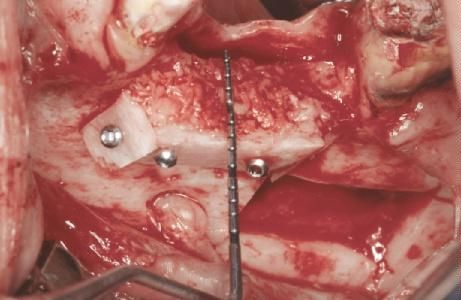
\includegraphics[width=221.1024pt,height=143.7732pt]{latexImage_0df1cbd9ddbc301d2d45b3a593fcdf3d.png}}
\put(285.4724,-222.8522){\fontsize{9}{1}\usefont{T1}{cmr}{m}{n}\selectfont\color{color_112230}Fig 3-1b  Blood vessels running perpendicular to the }
\put(285.4724,-233.8502){\fontsize{9}{1}\usefont{T1}{cmr}{m}{n}\selectfont\color{color_72488}bone.}
\put(285.4725,-209.1182){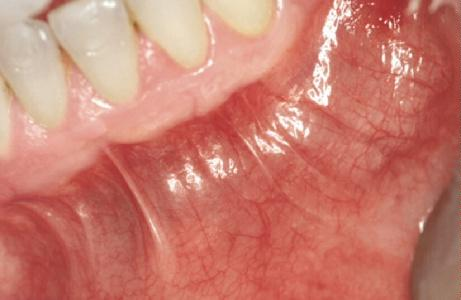
\includegraphics[width=221.1024pt,height=144.1855pt]{latexImage_df37646ba9a3781b6fd1ddad167a09b4.png}}
\put(293.6436,-585.7559){\fontsize{10.8}{1}\usefont{T1}{cmr}{m}{n}\selectfont\color{color_112230} nIncisions have to take into consideration }
\put(302.478,-600.7571){\fontsize{10.8}{1}\usefont{T1}{cmr}{m}{n}\selectfont\color{color_72488}the course of the blood vessels, on the one }
\put(302.478,-615.7583){\fontsize{10.8}{1}\usefont{T1}{cmr}{m}{n}\selectfont\color{color_72488}hand retaining the maximum vasculariza}
\put(502.9789,-615.7562){\fontsize{10.8}{1}\usefont{T1}{cmr}{m}{n}\selectfont\color{color_72488}-}
\put(302.4812,-630.7563){\fontsize{10.8}{1}\usefont{T1}{cmr}{m}{n}\selectfont\color{color_72488}tion of the flap, and on the other, avoiding }
\put(302.4812,-645.7574){\fontsize{10.8}{1}\usefont{T1}{cmr}{m}{n}\selectfont\color{color_72488}heavy bleeding during the surgery (Fig}
\put(481.2528,-645.7571){\fontsize{10.8}{1}\usefont{T1}{cmr}{m}{n}\selectfont\color{color_72488} 3-1c }
\put(302.4804,-660.7583){\fontsize{10.8}{1}\usefont{T1}{cmr}{m}{n}\selectfont\color{color_72488}and d).}
\put(293.43,-675.7595){\fontsize{10.8}{1}\usefont{T1}{cmr}{m}{n}\selectfont\color{color_112230} nIncisions and flap design must offer the best }
\put(302.4804,-690.7607){\fontsize{10.8}{1}\usefont{T1}{cmr}{m}{n}\selectfont\color{color_72488}possible vision and access for the surgeon.}
\put(293.484,-705.7619){\fontsize{10.8}{1}\usefont{T1}{cmr}{m}{n}\selectfont\color{color_112230} nIncisions must offer a wide flap basis to re}
\put(502.9781,-705.7554){\fontsize{10.8}{1}\usefont{T1}{cmr}{m}{n}\selectfont\color{color_72488}-}
\put(302.4804,-720.7556){\fontsize{10.8}{1}\usefont{T1}{cmr}{m}{n}\selectfont\color{color_72488}duce the risk of flap necrosis.}
\put(50.1969,-417.3137){\fontsize{9}{1}\usefont{T1}{cmr}{m}{n}\selectfont\color{color_112230}Fig 3-1c  Important ramifications of the lingual artery in }
\put(50.1969,-428.3117){\fontsize{9}{1}\usefont{T1}{cmr}{m}{n}\selectfont\color{color_72488}the mandibular anterior area.}
\put(50.1969,-403.3605){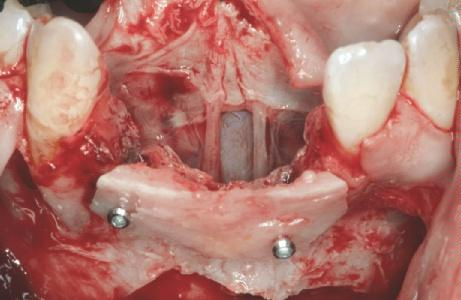
\includegraphics[width=221.1024pt,height=143.8293pt]{latexImage_a5be94fd68d5311828d7210d8f287859.png}}
\put(50.1969,-505.3749){\fontsize{9}{1}\usefont{T1}{cmr}{m}{n}\selectfont\color{color_112230}Fig 3-1d  Typical incision in the middle of the crest in the }
\put(50.1969,-516.3729){\fontsize{9}{1}\usefont{T1}{cmr}{m}{n}\selectfont\color{color_72488}edentulous maxilla, with the releasing incision in the fren-}
\put(50.19691,-527.3708){\fontsize{9}{1}\usefont{T1}{cmr}{m}{n}\selectfont\color{color_72488}ulum for implant and augmentation surgery, preserving a }
\put(50.19691,-538.3689){\fontsize{9}{1}\usefont{T1}{cmr}{m}{n}\selectfont\color{color_72488}sufficient vascular supply for good postoperative healing.}
\put(285.4725,-539.511){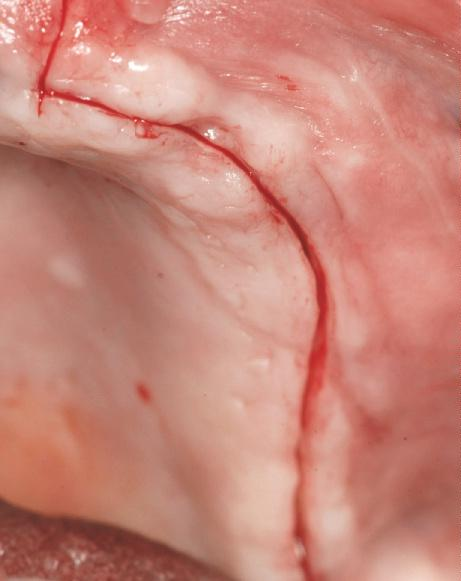
\includegraphics[width=221.1024pt,height=278.9313pt]{latexImage_9127a55f985cc72abf2645e3e7d4ab47.png}}
\end{picture}
\newpage
\begin{tikzpicture}[overlay]\path(0pt,0pt);\end{tikzpicture}
\begin{picture}(-5,0)(2.5,0)
\put(58.7009,-754.1789){\fontsize{11}{1}\usefont{T1}{cmr}{m}{n}\selectfont\color{color_112230}82}
\put(58.7009,-29.88385){\fontsize{11}{1}\usefont{T1}{cmr}{m}{n}\selectfont\color{color_112230}3}
\put(64.9269,-29.88391){\fontsize{11}{1}\usefont{T1}{cmr}{m}{n}\selectfont\color{color_112230} Soft tissue management and bone augmentation in implantology}
\put(66.7099,-300.7559){\fontsize{10.8}{1}\usefont{T1}{cmr}{m}{n}\selectfont\color{color_112230} nIncisions and flap design should reduce the }
\put(75.7063,-315.7571){\fontsize{10.8}{1}\usefont{T1}{cmr}{m}{n}\selectfont\color{color_72488}risk of scar tissue, especially in the esthetic }
\put(75.7063,-330.7583){\fontsize{10.8}{1}\usefont{T1}{cmr}{m}{n}\selectfont\color{color_72488}area (Fig 3-1e).}
\put(66.7099,-345.7595){\fontsize{10.8}{1}\usefont{T1}{cmr}{m}{n}\selectfont\color{color_112230} nAtraumatic incisions, flap preparation, and }
\put(75.7063,-360.7607){\fontsize{10.8}{1}\usefont{T1}{cmr}{m}{n}\selectfont\color{color_72488}sutures without any tension are important }
\put(75.7063,-375.7619){\fontsize{10.8}{1}\usefont{T1}{cmr}{m}{n}\selectfont\color{color_72488}factors to reduce the risk of flap necrosis }
\put(75.7063,-390.7631){\fontsize{10.8}{1}\usefont{T1}{cmr}{m}{n}\selectfont\color{color_72488}(Fig 3-1f). }
\put(58.6963,-420.7655){\fontsize{10.8}{1}\usefont{T1}{cmr}{m}{n}\selectfont\color{color_72488}Two wound-healing processes are distinguished }
\put(58.6963,-435.7667){\fontsize{10.8}{1}\usefont{T1}{cmr}{m}{n}\selectfont\color{color_72488}in the context of exposure measures. In the case }
\put(58.6963,-450.7679){\fontsize{10.8}{1}\usefont{T1}{cmr}{m}{n}\selectfont\color{color_72488}of primary wound healing (per primam intentio}
\put(276.2072,-450.756){\fontsize{10.8}{1}\usefont{T1}{cmr}{m}{n}\selectfont\color{color_72488}-}
\put(58.7017,-465.7561){\fontsize{10.8}{1}\usefont{T1}{cmr}{m}{n}\selectfont\color{color_72488}nem), the wound margins should be correctly re-}
\put(58.7017,-480.7563){\fontsize{10.8}{1}\usefont{T1}{cmr}{m}{n}\selectfont\color{color_72488}positioned throughout, which results in the di-}
\put(58.7017,-495.7564){\fontsize{10.8}{1}\usefont{T1}{cmr}{m}{n}\selectfont\color{color_72488}rect closure of the superficial wound layers }
\put(58.7017,-510.7576){\fontsize{10.8}{1}\usefont{T1}{cmr}{m}{n}\selectfont\color{color_72488}through the formation of a fibrin network, with }
\put(58.7017,-525.7588){\fontsize{10.8}{1}\usefont{T1}{cmr}{m}{n}\selectfont\color{color_72488}optimal fibrinogen synthesis and neoangiogene}
\put(276.2072,-525.7566){\fontsize{10.8}{1}\usefont{T1}{cmr}{m}{n}\selectfont\color{color_72488}-}
\put(58.7017,-540.7567){\fontsize{10.8}{1}\usefont{T1}{cmr}{m}{n}\selectfont\color{color_72488}sis. The tensile strength of the tissue is, however, }
\put(58.7017,-555.7579){\fontsize{10.8}{1}\usefont{T1}{cmr}{m}{n}\selectfont\color{color_72488}only restored after the complete healing of the }
\put(58.7017,-570.7591){\fontsize{10.8}{1}\usefont{T1}{cmr}{m}{n}\selectfont\color{color_72488}submucosa after about 1 to 3}
\put(192.0593,-570.7583){\fontsize{10.8}{1}\usefont{T1}{cmr}{m}{n}\selectfont\color{color_72488} weeks. In contrast, }
\put(58.70089,-585.7595){\fontsize{10.8}{1}\usefont{T1}{cmr}{m}{n}\selectfont\color{color_72488}submucosal granulation tissue grows over tissue }
\put(58.70089,-600.7607){\fontsize{10.8}{1}\usefont{T1}{cmr}{m}{n}\selectfont\color{color_72488}continuity defects in the case of secondary }
\put(58.70089,-615.7619){\fontsize{10.8}{1}\usefont{T1}{cmr}{m}{n}\selectfont\color{color_72488}wound healing (per secundam intentionem), }
\put(58.7009,-630.7631){\fontsize{10.8}{1}\usefont{T1}{cmr}{m}{n}\selectfont\color{color_72488}which is determined by neutrophil polymorpho}
\put(276.2064,-630.7556){\fontsize{10.8}{1}\usefont{T1}{cmr}{m}{n}\selectfont\color{color_72488}-}
\put(58.69982,-645.7557){\fontsize{10.8}{1}\usefont{T1}{cmr}{m}{n}\selectfont\color{color_72488}nuclear leukocytes and macrophages until the }
\put(58.69982,-660.7569){\fontsize{10.8}{1}\usefont{T1}{cmr}{m}{n}\selectfont\color{color_72488}final epithelialization of the wound.}
\put(293.9764,-301.6311){\fontsize{12.5}{1}\usefont{T1}{cmr}{m}{n}\selectfont\color{color_112230}3.2.1 Cellular and molecular healing }
\put(333.6639,-316.1311){\fontsize{12.5}{1}\usefont{T1}{cmr}{m}{n}\selectfont\color{color_112230}mechanisms}
\put(293.9764,-345.7559){\fontsize{10.8}{1}\usefont{T1}{cmr}{m}{n}\selectfont\color{color_72488}Wound healing involves both the repair and the }
\put(293.9764,-360.7571){\fontsize{10.8}{1}\usefont{T1}{cmr}{m}{n}\selectfont\color{color_72488}regeneration of the damaged tissue. The inflam}
\put(511.4819,-360.756){\fontsize{10.8}{1}\usefont{T1}{cmr}{m}{n}\selectfont\color{color_72488}-}
\put(293.9764,-375.7562){\fontsize{10.8}{1}\usefont{T1}{cmr}{m}{n}\selectfont\color{color_72488}matory healing process mainly consists of reep-}
\put(293.9764,-390.7563){\fontsize{10.8}{1}\usefont{T1}{cmr}{m}{n}\selectfont\color{color_72488}ithelialization, neoangiogenesis, and the activa-}
\put(293.9764,-405.7564){\fontsize{10.8}{1}\usefont{T1}{cmr}{m}{n}\selectfont\color{color_72488}tion of connective tissue cells, which also gives }
\put(293.9764,-420.7576){\fontsize{10.8}{1}\usefont{T1}{cmr}{m}{n}\selectfont\color{color_72488}rise to the degradation of the proteins in the }
\put(293.9764,-435.7588){\fontsize{10.8}{1}\usefont{T1}{cmr}{m}{n}\selectfont\color{color_72488}extracellular matrix and their resynthesis.}
\put(503.2659,-433.0558){\fontsize{6.48}{1}\usefont{T1}{cmr}{m}{n}\selectfont\color{color_72488}159}
\put(515.0787,-435.7559){\fontsize{10.8}{1}\usefont{T1}{cmr}{m}{n}\selectfont\color{color_72488} }
\put(293.9811,-450.7571){\fontsize{10.8}{1}\usefont{T1}{cmr}{m}{n}\selectfont\color{color_72488}The regulation of these processes is determined }
\put(293.9811,-465.7583){\fontsize{10.8}{1}\usefont{T1}{cmr}{m}{n}\selectfont\color{color_72488}by interactions between proteins of the matrix }
\put(293.9811,-480.7595){\fontsize{10.8}{1}\usefont{T1}{cmr}{m}{n}\selectfont\color{color_72488}and epithelial cells as well as cytokines and }
\put(293.9811,-495.7607){\fontsize{10.8}{1}\usefont{T1}{cmr}{m}{n}\selectfont\color{color_72488}growth factors. After these three wound-healing }
\put(293.9811,-510.7618){\fontsize{10.8}{1}\usefont{T1}{cmr}{m}{n}\selectfont\color{color_72488}phases are complete, the result is either an area }
\put(293.9811,-525.7631){\fontsize{10.8}{1}\usefont{T1}{cmr}{m}{n}\selectfont\color{color_72488}of scar tissue formed by repair healing or an }
\put(293.9811,-540.7643){\fontsize{10.8}{1}\usefont{T1}{cmr}{m}{n}\selectfont\color{color_72488}area of exact regeneration by original morpho}
\put(511.4823,-540.7556){\fontsize{10.8}{1}\usefont{T1}{cmr}{m}{n}\selectfont\color{color_72488}-}
\put(293.9768,-555.7557){\fontsize{10.8}{1}\usefont{T1}{cmr}{m}{n}\selectfont\color{color_72488}logically functional tissue.}
\put(293.9764,-584.4252){\fontsize{11.5}{1}\usefont{T1}{cmr}{m}{n}\selectfont\color{color_112230}3.2.1.1 Inflammation phase (day 0 to 3)}
\put(293.9764,-600.7559){\fontsize{10.8}{1}\usefont{T1}{cmr}{m}{n}\selectfont\color{color_72488}A brief vasoconstriction and the formation of }
\put(293.9764,-615.7571){\fontsize{10.8}{1}\usefont{T1}{cmr}{m}{n}\selectfont\color{color_72488}the blood clot from a plasmatic network of }
\put(293.9764,-630.7583){\fontsize{10.8}{1}\usefont{T1}{cmr}{m}{n}\selectfont\color{color_72488}thrombocytes and erythrocytes is followed by }
\put(293.9764,-645.7595){\fontsize{10.8}{1}\usefont{T1}{cmr}{m}{n}\selectfont\color{color_72488}increased vascular permeability and the release }
\put(293.9764,-660.7607){\fontsize{10.8}{1}\usefont{T1}{cmr}{m}{n}\selectfont\color{color_72488}of cytokines. The fibrinogen synthesis in the }
\put(293.9764,-675.7619){\fontsize{10.8}{1}\usefont{T1}{cmr}{m}{n}\selectfont\color{color_72488}blood clot polymerizes fibrin and stimulates the }
\put(293.9764,-690.7631){\fontsize{10.8}{1}\usefont{T1}{cmr}{m}{n}\selectfont\color{color_72488}migration and proliferation of marginal epithe}
\put(511.4819,-690.7556){\fontsize{10.8}{1}\usefont{T1}{cmr}{m}{n}\selectfont\color{color_72488}-}
\put(293.9764,-705.7557){\fontsize{10.8}{1}\usefont{T1}{cmr}{m}{n}\selectfont\color{color_72488}lial cells. Thrombocytes also release chemotac-}
\put(293.9764,-720.7558){\fontsize{10.8}{1}\usefont{T1}{cmr}{m}{n}\selectfont\color{color_72488}tic cytokines such as TNF-α and IL-1 for neu-}
\put(58.7009,-222.8522){\fontsize{9}{1}\usefont{T1}{cmr}{m}{n}\selectfont\color{color_112230}Fig 3-1e  Intensive scar tissue formation in the maxillary }
\put(58.7009,-233.8502){\fontsize{9}{1}\usefont{T1}{cmr}{m}{n}\selectfont\color{color_72488}anterior area after horizontal incisions (further }
\put(58.7009,-244.8482){\fontsize{9}{1}\usefont{T1}{cmr}{m}{n}\selectfont\color{color_72488}apicoectomies).}
\put(58.70083,-209.0306){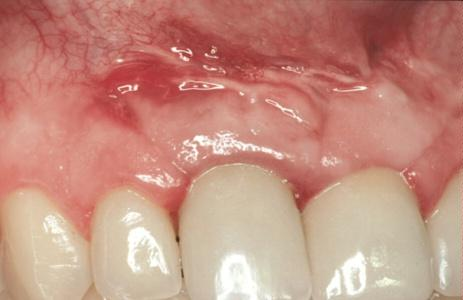
\includegraphics[width=222.24pt,height=144pt]{latexImage_70fa6bf0660974fe8586ea275d0c47d8.png}}
\put(293.9764,-222.8522){\fontsize{9}{1}\usefont{T1}{cmr}{m}{n}\selectfont\color{color_112230}Fig 3-1f  Clinical situation in the right mandible 2 weeks }
\put(293.9764,-233.8502){\fontsize{9}{1}\usefont{T1}{cmr}{m}{n}\selectfont\color{color_72488}postoperatively: incision in the middle of the crest sutured }
\put(293.9764,-244.8482){\fontsize{9}{1}\usefont{T1}{cmr}{m}{n}\selectfont\color{color_72488}with 6-0 monofilament resorbable sutures.}
\put(293.9764,-208.8719){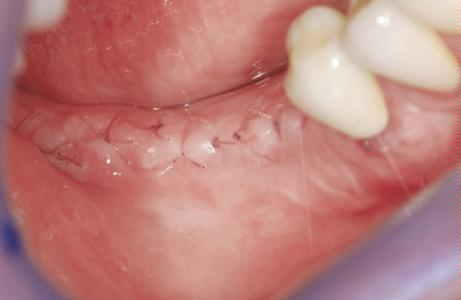
\includegraphics[width=221.1023pt,height=143.7753pt]{latexImage_0d32a5f1b2b65f8541794ef298e222e5.png}}
\end{picture}
\newpage
\begin{tikzpicture}[overlay]\path(0pt,0pt);\end{tikzpicture}
\begin{picture}(-5,0)(2.5,0)
\put(493.133,-754.1789){\fontsize{11}{1}\usefont{T1}{cmr}{m}{n}\selectfont\color{color_112230}83}
\put(144.862,-29.88385){\fontsize{11}{1}\usefont{T1}{cmr}{m}{n}\selectfont\color{color_112230}3.2}
\put(161.989,-29.88391){\fontsize{11}{1}\usefont{T1}{cmr}{m}{n}\selectfont\color{color_112230} The basics of incisions, suturing techniques, and soft tissue healing}
\put(50.1969,-75.75592){\fontsize{10.8}{1}\usefont{T1}{cmr}{m}{n}\selectfont\color{color_72488}trophil granulocytes and macrophages.}
\put(238.2051,-73.05591){\fontsize{6.48}{1}\usefont{T1}{cmr}{m}{n}\selectfont\color{color_72488}79}
\put(246.1236,-75.75592){\fontsize{10.8}{1}\usefont{T1}{cmr}{m}{n}\selectfont\color{color_72488} This }
\put(50.2008,-90.75714){\fontsize{10.8}{1}\usefont{T1}{cmr}{m}{n}\selectfont\color{color_72488}immune response decontaminates the wound }
\put(50.2008,-105.7584){\fontsize{10.8}{1}\usefont{T1}{cmr}{m}{n}\selectfont\color{color_72488}by way of phagocytosis, cell-mediated immune }
\put(50.2008,-120.7596){\fontsize{10.8}{1}\usefont{T1}{cmr}{m}{n}\selectfont\color{color_72488}response, and peroxides, before lymphocyte-re}
\put(267.7031,-120.7563){\fontsize{10.8}{1}\usefont{T1}{cmr}{m}{n}\selectfont\color{color_72488}-}
\put(50.19755,-135.7565){\fontsize{10.8}{1}\usefont{T1}{cmr}{m}{n}\selectfont\color{color_72488}cruiting macrophages enter the tissue. The }
\put(50.19755,-150.7577){\fontsize{10.8}{1}\usefont{T1}{cmr}{m}{n}\selectfont\color{color_72488}lymphocytic reaction follows antigen presenta}
\put(267.7031,-150.7566){\fontsize{10.8}{1}\usefont{T1}{cmr}{m}{n}\selectfont\color{color_72488}-}
\put(50.19755,-165.7567){\fontsize{10.8}{1}\usefont{T1}{cmr}{m}{n}\selectfont\color{color_72488}tion specific to the molecular patterns of vari-}
\put(50.19755,-180.7568){\fontsize{10.8}{1}\usefont{T1}{cmr}{m}{n}\selectfont\color{color_72488}ous microorganisms.}
\put(50.1969,-207.4252){\fontsize{11.5}{1}\usefont{T1}{cmr}{m}{n}\selectfont\color{color_112230}3.2.1.2 Proliferative and fibroblastic phase }
\put(89.8834,-223.4218){\fontsize{11.5}{1}\usefont{T1}{cmr}{m}{n}\selectfont\color{color_112230}(day 3 to 12)}
\put(50.1969,-240.7559){\fontsize{10.8}{1}\usefont{T1}{cmr}{m}{n}\selectfont\color{color_72488}The proliferation and migration activity of fibro-}
\put(50.19691,-255.756){\fontsize{10.8}{1}\usefont{T1}{cmr}{m}{n}\selectfont\color{color_72488}blasts is enhanced by growth factors expressed }
\put(50.19691,-270.7573){\fontsize{10.8}{1}\usefont{T1}{cmr}{m}{n}\selectfont\color{color_72488}by macrophages and leads to increased colla}
\put(267.7024,-270.7562){\fontsize{10.8}{1}\usefont{T1}{cmr}{m}{n}\selectfont\color{color_72488}-}
\put(50.19691,-285.7563){\fontsize{10.8}{1}\usefont{T1}{cmr}{m}{n}\selectfont\color{color_72488}gen synthesis and to neoangiogenesis triggered }
\put(50.19691,-300.7575){\fontsize{10.8}{1}\usefont{T1}{cmr}{m}{n}\selectfont\color{color_72488}by VEGF and β-FGF.}
\put(148.3955,-298.0559){\fontsize{6.48}{1}\usefont{T1}{cmr}{m}{n}\selectfont\color{color_72488}168}
\put(160.2731,-300.7559){\fontsize{10.8}{1}\usefont{T1}{cmr}{m}{n}\selectfont\color{color_72488} The reepithelialization }
\put(50.19949,-315.7571){\fontsize{10.8}{1}\usefont{T1}{cmr}{m}{n}\selectfont\color{color_72488}of the wound margins restores the integrity of }
\put(50.19949,-330.7583){\fontsize{10.8}{1}\usefont{T1}{cmr}{m}{n}\selectfont\color{color_72488}the anatomical structures. Integrins function }
\put(50.19949,-345.7595){\fontsize{10.8}{1}\usefont{T1}{cmr}{m}{n}\selectfont\color{color_72488}as receptors for chemotactic factors, which in}
\put(267.7029,-345.7563){\fontsize{10.8}{1}\usefont{T1}{cmr}{m}{n}\selectfont\color{color_72488}-}
\put(50.19733,-360.7564){\fontsize{10.8}{1}\usefont{T1}{cmr}{m}{n}\selectfont\color{color_72488}teract with collagen and fibronectin, and PDGF }
\put(50.19733,-375.7576){\fontsize{10.8}{1}\usefont{T1}{cmr}{m}{n}\selectfont\color{color_72488}of thrombocytes and TGF-β of macrophages }
\put(50.1969,-390.7583){\fontsize{10.8}{1}\usefont{T1}{cmr}{m}{n}\selectfont\color{color_72488} activate mesenchymal cells and thereby the }
\put(50.1969,-405.7595){\fontsize{10.8}{1}\usefont{T1}{cmr}{m}{n}\selectfont\color{color_72488}formation of granulation tissue.}
\put(198.3925,-403.0559){\fontsize{6.48}{1}\usefont{T1}{cmr}{m}{n}\selectfont\color{color_72488}44,79}
\put(216.2057,-405.7559){\fontsize{10.8}{1}\usefont{T1}{cmr}{m}{n}\selectfont\color{color_72488} Glyco sa mi-}
\put(50.1989,-420.7571){\fontsize{10.8}{1}\usefont{T1}{cmr}{m}{n}\selectfont\color{color_72488}no  glycans, proteoglycans, tenascin, and throm-}
\put(50.1989,-435.7583){\fontsize{10.8}{1}\usefont{T1}{cmr}{m}{n}\selectfont\color{color_72488}bospondin invade the extracellular matrix, and }
\put(50.1989,-450.7595){\fontsize{10.8}{1}\usefont{T1}{cmr}{m}{n}\selectfont\color{color_72488}myofibroblasts differentiate to contract the }
\put(50.1989,-465.7607){\fontsize{10.8}{1}\usefont{T1}{cmr}{m}{n}\selectfont\color{color_72488}wound area.}
\put(50.1969,-494.4252){\fontsize{11.5}{1}\usefont{T1}{cmr}{m}{n}\selectfont\color{color_112230}3.2.1.3 Maturation phase (day 6 to 14)}
\put(50.1969,-510.7559){\fontsize{10.8}{1}\usefont{T1}{cmr}{m}{n}\selectfont\color{color_72488}Matrix metalloproteinases trigger collagenolysis }
\put(50.1969,-525.7571){\fontsize{10.8}{1}\usefont{T1}{cmr}{m}{n}\selectfont\color{color_72488}and synthesis in order to reorganize the extracel}
\put(267.7024,-525.756){\fontsize{10.8}{1}\usefont{T1}{cmr}{m}{n}\selectfont\color{color_72488}-}
\put(50.19691,-540.7562){\fontsize{10.8}{1}\usefont{T1}{cmr}{m}{n}\selectfont\color{color_72488}lular matrix and granulation tissue. The fibroblas-}
\put(50.19691,-555.7563){\fontsize{10.8}{1}\usefont{T1}{cmr}{m}{n}\selectfont\color{color_72488}tic phase is determined by the formation of }
\put(50.19691,-570.7575){\fontsize{10.8}{1}\usefont{T1}{cmr}{m}{n}\selectfont\color{color_72488}type III and I collagen and improves the tensile }
\put(50.19691,-585.7587){\fontsize{10.8}{1}\usefont{T1}{cmr}{m}{n}\selectfont\color{color_72488}strength and elasticity of the new tissue. Integ}
\put(267.7024,-585.7565){\fontsize{10.8}{1}\usefont{T1}{cmr}{m}{n}\selectfont\color{color_72488}-}
\put(50.19691,-600.7567){\fontsize{10.8}{1}\usefont{T1}{cmr}{m}{n}\selectfont\color{color_72488}rins in the cell membranes consolidate the provi-}
\put(50.19691,-615.7568){\fontsize{10.8}{1}\usefont{T1}{cmr}{m}{n}\selectfont\color{color_72488}sional matrix through α- and β-heterodimer pro-}
\put(50.19691,-630.7569){\fontsize{10.8}{1}\usefont{T1}{cmr}{m}{n}\selectfont\color{color_72488}teins and enable reepithelialization. Integrin }
\put(50.19689,-645.7581){\fontsize{10.8}{1}\usefont{T1}{cmr}{m}{n}\selectfont\color{color_72488}α5β1 not only stimulates adhesion and migration }
\put(50.19689,-660.7593){\fontsize{10.8}{1}\usefont{T1}{cmr}{m}{n}\selectfont\color{color_72488}in this process, but also has a decisive effect on }
\put(50.19689,-675.7605){\fontsize{10.8}{1}\usefont{T1}{cmr}{m}{n}\selectfont\color{color_72488}cell growth through signaling.}
\put(183.9052,-673.0559){\fontsize{6.48}{1}\usefont{T1}{cmr}{m}{n}\selectfont\color{color_72488}12,86,109}
\put(285.4725,-75.14288){\fontsize{12.5}{1}\usefont{T1}{cmr}{m}{n}\selectfont\color{color_112230}3.2.2 The reactions of tissue to sutures}
\put(285.4725,-105.756){\fontsize{10.8}{1}\usefont{T1}{cmr}{m}{n}\selectfont\color{color_72488}Suture materials are a foreign body and inevita-}
\put(285.4725,-120.7561){\fontsize{10.8}{1}\usefont{T1}{cmr}{m}{n}\selectfont\color{color_72488}bly lead to mild inflammatory reactions in tissue, }
\put(285.4725,-135.7573){\fontsize{10.8}{1}\usefont{T1}{cmr}{m}{n}\selectfont\color{color_72488}which may locally reduce resistance to infec}
\put(502.978,-135.7562){\fontsize{10.8}{1}\usefont{T1}{cmr}{m}{n}\selectfont\color{color_72488}-}
\put(285.4725,-150.7563){\fontsize{10.8}{1}\usefont{T1}{cmr}{m}{n}\selectfont\color{color_72488}tions. Specifically, needle and thread penetration }
\put(285.4725,-165.7576){\fontsize{10.8}{1}\usefont{T1}{cmr}{m}{n}\selectfont\color{color_72488}sites represent biologic niches where bacterial }
\put(285.4725,-180.7588){\fontsize{10.8}{1}\usefont{T1}{cmr}{m}{n}\selectfont\color{color_72488}invasions are possible.}
\put(388.2872,-178.056){\fontsize{6.48}{1}\usefont{T1}{cmr}{m}{n}\selectfont\color{color_72488}6}
\put(299.6457,-195.756){\fontsize{10.8}{1}\usefont{T1}{cmr}{m}{n}\selectfont\color{color_72488}Wound healing in the oral cavity involves a }
\put(285.4761,-210.7572){\fontsize{10.8}{1}\usefont{T1}{cmr}{m}{n}\selectfont\color{color_72488}higher risk of bacterial contamination, the so-}
\put(285.4761,-225.7584){\fontsize{10.8}{1}\usefont{T1}{cmr}{m}{n}\selectfont\color{color_72488}called ‘wick effect.’ Biofilm formation therefore }
\put(285.4761,-240.7596){\fontsize{10.8}{1}\usefont{T1}{cmr}{m}{n}\selectfont\color{color_72488}needs to be reduced as much as possible by }
\put(285.4761,-255.7609){\fontsize{10.8}{1}\usefont{T1}{cmr}{m}{n}\selectfont\color{color_72488}using monofilament threads. Suture materials }
\put(285.4761,-270.7621){\fontsize{10.8}{1}\usefont{T1}{cmr}{m}{n}\selectfont\color{color_72488}must possess high tensile strength and tear re}
\put(502.9784,-270.7556){\fontsize{10.8}{1}\usefont{T1}{cmr}{m}{n}\selectfont\color{color_72488}-}
\put(285.4729,-285.7557){\fontsize{10.8}{1}\usefont{T1}{cmr}{m}{n}\selectfont\color{color_72488}sistance, good knotting characteristics, and high }
\put(285.4729,-300.7569){\fontsize{10.8}{1}\usefont{T1}{cmr}{m}{n}\selectfont\color{color_72488}knot strength.}
\put(350.9181,-298.056){\fontsize{6.48}{1}\usefont{T1}{cmr}{m}{n}\selectfont\color{color_72488}174}
\put(362.6013,-300.756){\fontsize{10.8}{1}\usefont{T1}{cmr}{m}{n}\selectfont\color{color_72488} In this context, it was shown }
\put(285.4677,-315.7572){\fontsize{10.8}{1}\usefont{T1}{cmr}{m}{n}\selectfont\color{color_72488}that atraumatic microsurgical application sig}
\put(502.9786,-315.7561){\fontsize{10.8}{1}\usefont{T1}{cmr}{m}{n}\selectfont\color{color_72488}-}
\put(285.4731,-330.7563){\fontsize{10.8}{1}\usefont{T1}{cmr}{m}{n}\selectfont\color{color_72488}nificantly supports flap and wound healing.}
\put(498.7212,-328.0559){\fontsize{6.48}{1}\usefont{T1}{cmr}{m}{n}\selectfont\color{color_72488}25}
\put(506.5748,-330.7559){\fontsize{10.8}{1}\usefont{T1}{cmr}{m}{n}\selectfont\color{color_72488} }
\put(285.4772,-345.7571){\fontsize{10.8}{1}\usefont{T1}{cmr}{m}{n}\selectfont\color{color_72488}The use of atraumatic monofilament suture }
\put(285.4772,-360.7583){\fontsize{10.8}{1}\usefont{T1}{cmr}{m}{n}\selectfont\color{color_72488}threads with a maximum thickness of 0.01 mm }
\put(285.4772,-375.7595){\fontsize{10.8}{1}\usefont{T1}{cmr}{m}{n}\selectfont\color{color_72488}(i.e. ≤ 6-0) is therefore indicated due to lower }
\put(285.4772,-390.7607){\fontsize{10.8}{1}\usefont{T1}{cmr}{m}{n}\selectfont\color{color_72488}levels of bacterial colonization,}
\put(428.6113,-388.0559){\fontsize{6.48}{1}\usefont{T1}{cmr}{m}{n}\selectfont\color{color_72488}114}
\put(440.2946,-390.7559){\fontsize{10.8}{1}\usefont{T1}{cmr}{m}{n}\selectfont\color{color_72488} smaller histo-}
\put(285.4734,-405.756){\fontsize{10.8}{1}\usefont{T1}{cmr}{m}{n}\selectfont\color{color_72488}logic inflammatory infiltrate, and the reduced }
\put(285.4734,-420.7572){\fontsize{10.8}{1}\usefont{T1}{cmr}{m}{n}\selectfont\color{color_72488}formation of scar tissue. At the time of the re}
\put(502.9789,-420.7562){\fontsize{10.8}{1}\usefont{T1}{cmr}{m}{n}\selectfont\color{color_72488}-}
\put(285.4734,-435.7563){\fontsize{10.8}{1}\usefont{T1}{cmr}{m}{n}\selectfont\color{color_72488}moval of the sutures after 14}
\put(420.5697,-435.7559){\fontsize{10.8}{1}\usefont{T1}{cmr}{m}{n}\selectfont\color{color_72488} days, the epitheli-}
\put(285.4725,-450.756){\fontsize{10.8}{1}\usefont{T1}{cmr}{m}{n}\selectfont\color{color_72488}um is already keratinized,}
\put(407.9117,-448.0559){\fontsize{6.48}{1}\usefont{T1}{cmr}{m}{n}\selectfont\color{color_72488}159}
\put(419.5949,-450.7559){\fontsize{10.8}{1}\usefont{T1}{cmr}{m}{n}\selectfont\color{color_72488} and the thread is }
\put(285.4697,-465.7571){\fontsize{10.8}{1}\usefont{T1}{cmr}{m}{n}\selectfont\color{color_72488}slightly colonized by rod- and spindle-shaped }
\put(285.4697,-480.7583){\fontsize{10.8}{1}\usefont{T1}{cmr}{m}{n}\selectfont\color{color_72488}bacteria. Due to the complex, multilevel sutur}
\put(502.9784,-480.7561){\fontsize{10.8}{1}\usefont{T1}{cmr}{m}{n}\selectfont\color{color_72488}-}
\put(285.4729,-495.7563){\fontsize{10.8}{1}\usefont{T1}{cmr}{m}{n}\selectfont\color{color_72488}ing techniques used to achieve esthetic and }
\put(285.4729,-510.7574){\fontsize{10.8}{1}\usefont{T1}{cmr}{m}{n}\selectfont\color{color_72488}functional results, it is recommended to use re}
\put(502.9784,-510.7563){\fontsize{10.8}{1}\usefont{T1}{cmr}{m}{n}\selectfont\color{color_72488}-}
\put(285.4729,-525.7565){\fontsize{10.8}{1}\usefont{T1}{cmr}{m}{n}\selectfont\color{color_72488}sorbable suture threads. Nevertheless, as the }
\put(285.4729,-540.7577){\fontsize{10.8}{1}\usefont{T1}{cmr}{m}{n}\selectfont\color{color_72488}metabolic degradation process takes approxi}
\put(502.9784,-540.7566){\fontsize{10.8}{1}\usefont{T1}{cmr}{m}{n}\selectfont\color{color_72488}-}
\put(285.4729,-555.7567){\fontsize{10.8}{1}\usefont{T1}{cmr}{m}{n}\selectfont\color{color_72488}mately 60}
\put(332.6253,-555.7559){\fontsize{10.8}{1}\usefont{T1}{cmr}{m}{n}\selectfont\color{color_72488} days, these should be removed if ac-}
\put(285.4725,-570.756){\fontsize{10.8}{1}\usefont{T1}{cmr}{m}{n}\selectfont\color{color_72488}cessible after 14}
\put(367.5849,-570.7559){\fontsize{10.8}{1}\usefont{T1}{cmr}{m}{n}\selectfont\color{color_72488} days. This results in greater }
\put(285.4725,-585.7571){\fontsize{10.8}{1}\usefont{T1}{cmr}{m}{n}\selectfont\color{color_72488}patient comfort and is obligatory in the particu}
\put(502.978,-585.756){\fontsize{10.8}{1}\usefont{T1}{cmr}{m}{n}\selectfont\color{color_72488}-}
\put(285.4725,-600.7562){\fontsize{10.8}{1}\usefont{T1}{cmr}{m}{n}\selectfont\color{color_72488}lar case of two-layer wound closure. The surgical }
\put(285.4725,-615.7573){\fontsize{10.8}{1}\usefont{T1}{cmr}{m}{n}\selectfont\color{color_72488}needle should have a curve length of 11 to }
\put(285.4725,-630.7585){\fontsize{10.8}{1}\usefont{T1}{cmr}{m}{n}\selectfont\color{color_72488}13}
\put(298.4541,-630.7584){\fontsize{10.8}{1}\usefont{T1}{cmr}{m}{n}\selectfont\color{color_72488} mm, and a triangular profile sharpened and }
\put(285.4725,-645.7596){\fontsize{10.8}{1}\usefont{T1}{cmr}{m}{n}\selectfont\color{color_72488}polished toward the tip. The needle should be }
\put(285.4725,-660.7608){\fontsize{10.8}{1}\usefont{T1}{cmr}{m}{n}\selectfont\color{color_72488}made of stainless steel to achieve the best pos}
\put(502.978,-660.7565){\fontsize{10.8}{1}\usefont{T1}{cmr}{m}{n}\selectfont\color{color_72488}-}
\put(285.4725,-675.7566){\fontsize{10.8}{1}\usefont{T1}{cmr}{m}{n}\selectfont\color{color_72488}sible stability while causing the least possible }
\put(285.4725,-690.7578){\fontsize{10.8}{1}\usefont{T1}{cmr}{m}{n}\selectfont\color{color_72488}trauma to the tissue (Fig}
\put(399.8531,-690.7572){\fontsize{10.8}{1}\usefont{T1}{cmr}{m}{n}\selectfont\color{color_72488} 3-2a to d).}
\end{picture}
\newpage
\begin{tikzpicture}[overlay]\path(0pt,0pt);\end{tikzpicture}
\begin{picture}(-5,0)(2.5,0)
\put(58.7009,-754.1789){\fontsize{11}{1}\usefont{T1}{cmr}{m}{n}\selectfont\color{color_112230}84}
\put(58.7009,-29.88385){\fontsize{11}{1}\usefont{T1}{cmr}{m}{n}\selectfont\color{color_112230}3}
\put(64.9269,-29.88391){\fontsize{11}{1}\usefont{T1}{cmr}{m}{n}\selectfont\color{color_112230} Soft tissue management and bone augmentation in implantology}
\put(58.7008,-513.0172){\fontsize{14}{1}\usefont{T1}{cmr}{m}{n}\selectfont\color{color_112230}3.3 Instruments}
\put(58.7008,-540.7559){\fontsize{10.8}{1}\usefont{T1}{cmr}{m}{n}\selectfont\color{color_72488}Microsurgical concepts have become estab-}
\put(58.7008,-555.756){\fontsize{10.8}{1}\usefont{T1}{cmr}{m}{n}\selectfont\color{color_72488}lished in soft tissue management.}
\put(223.3898,-553.0559){\fontsize{6.48}{1}\usefont{T1}{cmr}{m}{n}\selectfont\color{color_72488}46,189}
\put(245.1622,-555.7559){\fontsize{10.8}{1}\usefont{T1}{cmr}{m}{n}\selectfont\color{color_72488} Micro-}
\put(58.70019,-570.756){\fontsize{10.8}{1}\usefont{T1}{cmr}{m}{n}\selectfont\color{color_72488}surgery is understood to mean surgical proced-}
\put(58.70019,-585.7562){\fontsize{10.8}{1}\usefont{T1}{cmr}{m}{n}\selectfont\color{color_72488}ures that require optical magnification aids, }
\put(58.70019,-600.7574){\fontsize{10.8}{1}\usefont{T1}{cmr}{m}{n}\selectfont\color{color_72488}miniaturized instruments, and suturing mater}
\put(276.2068,-600.7563){\fontsize{10.8}{1}\usefont{T1}{cmr}{m}{n}\selectfont\color{color_72488}-}
\put(58.70019,-615.7564){\fontsize{10.8}{1}\usefont{T1}{cmr}{m}{n}\selectfont\color{color_72488}ials that have been adapted accordingly. The }
\put(58.70019,-630.7576){\fontsize{10.8}{1}\usefont{T1}{cmr}{m}{n}\selectfont\color{color_72488}atraumatic }
\put(112.3444,-630.7571){\fontsize{10.8}{1}\usefont{T1}{cmr}{m}{n}\selectfont\color{color_72488} management of tissue and the opti}
\put(276.2074,-630.756){\fontsize{10.8}{1}\usefont{T1}{cmr}{m}{n}\selectfont\color{color_72488}-}
\put(58.7008,-645.7562){\fontsize{10.8}{1}\usefont{T1}{cmr}{m}{n}\selectfont\color{color_72488}mal closure of wounds by way of microsurgical }
\put(58.7008,-660.7573){\fontsize{10.8}{1}\usefont{T1}{cmr}{m}{n}\selectfont\color{color_72488}techniques have produced significantly im}
\put(276.2074,-660.7563){\fontsize{10.8}{1}\usefont{T1}{cmr}{m}{n}\selectfont\color{color_72488}-}
\put(58.7008,-675.7564){\fontsize{10.8}{1}\usefont{T1}{cmr}{m}{n}\selectfont\color{color_72488}proved results. The improved and predictable }
\put(58.7008,-690.7576){\fontsize{10.8}{1}\usefont{T1}{cmr}{m}{n}\selectfont\color{color_72488}wound healing process was described by Bur}
\put(276.2074,-690.7565){\fontsize{10.8}{1}\usefont{T1}{cmr}{m}{n}\selectfont\color{color_72488}-}
\put(58.7008,-705.7566){\fontsize{10.8}{1}\usefont{T1}{cmr}{m}{n}\selectfont\color{color_72488}khardt and Lang,}
\put(140.0844,-703.0559){\fontsize{6.48}{1}\usefont{T1}{cmr}{m}{n}\selectfont\color{color_72488}25}
\put(148.0028,-705.7559){\fontsize{10.8}{1}\usefont{T1}{cmr}{m}{n}\selectfont\color{color_72488} who compared macrosurgi-}
\put(58.69976,-720.756){\fontsize{10.8}{1}\usefont{T1}{cmr}{m}{n}\selectfont\color{color_72488}cal and microsurgical procedures.}
\put(308.1473,-510.7608){\fontsize{10.8}{1}\usefont{T1}{cmr}{m}{n}\selectfont\color{color_72488}The shape of the instruments’ grip should be }
\put(293.9778,-525.762){\fontsize{10.8}{1}\usefont{T1}{cmr}{m}{n}\selectfont\color{color_72488}round and well-balanced and have a length of at }
\put(293.9778,-540.7632){\fontsize{10.8}{1}\usefont{T1}{cmr}{m}{n}\selectfont\color{color_72488}least 16}
\put(331.795,-540.7631){\fontsize{10.8}{1}\usefont{T1}{cmr}{m}{n}\selectfont\color{color_72488} cm. In particular, in the case of length}
\put(511.4822,-540.7555){\fontsize{10.8}{1}\usefont{T1}{cmr}{m}{n}\selectfont\color{color_72488}-}
\put(293.9767,-555.7556){\fontsize{10.8}{1}\usefont{T1}{cmr}{m}{n}\selectfont\color{color_72488}ier procedures, such ergonomic work in the pos-}
\put(293.9767,-570.7557){\fontsize{10.8}{1}\usefont{T1}{cmr}{m}{n}\selectfont\color{color_72488}terior sections of the jaw may have advantages. }
\put(293.9767,-585.757){\fontsize{10.8}{1}\usefont{T1}{cmr}{m}{n}\selectfont\color{color_72488}Grips with a round profile make possible the }
\put(293.9767,-600.7582){\fontsize{10.8}{1}\usefont{T1}{cmr}{m}{n}\selectfont\color{color_72488}significantly more precise manipulation of in}
\put(511.4833,-600.756){\fontsize{10.8}{1}\usefont{T1}{cmr}{m}{n}\selectfont\color{color_72488}-}
\put(293.9767,-615.7561){\fontsize{10.8}{1}\usefont{T1}{cmr}{m}{n}\selectfont\color{color_72488}struments in the pencil-grip position.}
\put(308.1463,-630.7573){\fontsize{10.8}{1}\usefont{T1}{cmr}{m}{n}\selectfont\color{color_72488}On the one hand, an incision without any }
\put(293.9767,-645.7585){\fontsize{10.8}{1}\usefont{T1}{cmr}{m}{n}\selectfont\color{color_72488}tissue loss is possible with a single-edged }
\put(293.9767,-660.7598){\fontsize{10.8}{1}\usefont{T1}{cmr}{m}{n}\selectfont\color{color_72488}No. 15c blade with a pointed tip and adequate }
\put(293.9767,-675.7609){\fontsize{10.8}{1}\usefont{T1}{cmr}{m}{n}\selectfont\color{color_72488}width in the case of two-layer dissections; on }
\put(293.9767,-690.7621){\fontsize{10.8}{1}\usefont{T1}{cmr}{m}{n}\selectfont\color{color_72488}the other hand, one could use a double-edged }
\put(293.9767,-705.7634){\fontsize{10.8}{1}\usefont{T1}{cmr}{m}{n}\selectfont\color{color_72488}SM69 micro scalpel. In the selection of raspa}
\put(511.4822,-705.7558){\fontsize{10.8}{1}\usefont{T1}{cmr}{m}{n}\selectfont\color{color_72488}-}
\put(293.9767,-720.7559){\fontsize{10.8}{1}\usefont{T1}{cmr}{m}{n}\selectfont\color{color_72488}tories (e.g. Partsch Raspatories), a slender de-}
\put(58.7009,-222.8522){\fontsize{9}{1}\usefont{T1}{cmr}{m}{n}\selectfont\color{color_112230}Fig 3-2a  Exposure of a 3D-form grafted bone in the anter-}
\put(58.7009,-233.8502){\fontsize{9}{1}\usefont{T1}{cmr}{m}{n}\selectfont\color{color_72488}ior maxilla 3 months postoperatively using the same incision }
\put(58.7009,-244.8482){\fontsize{9}{1}\usefont{T1}{cmr}{m}{n}\selectfont\color{color_72488}line that was made during the grafting procedure, including }
\put(58.7009,-255.8462){\fontsize{9}{1}\usefont{T1}{cmr}{m}{n}\selectfont\color{color_72488}the releasing incision in the mesial third of the canine.}
\put(58.70083,-208.8703){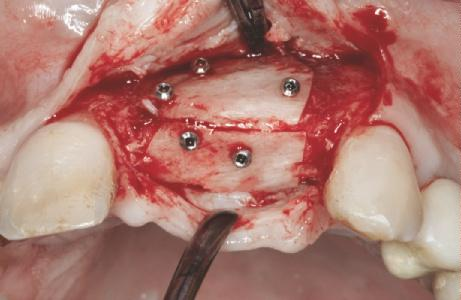
\includegraphics[width=221.1023pt,height=143.7724pt]{latexImage_6cdee2f471ec48d168bf71172d5c72eb.png}}
\put(293.9764,-222.8522){\fontsize{9}{1}\usefont{T1}{cmr}{m}{n}\selectfont\color{color_112230}Fig 3-2b  Insertion of two implants in the vertically grafted }
\put(293.9764,-233.8502){\fontsize{9}{1}\usefont{T1}{cmr}{m}{n}\selectfont\color{color_72488}bone.}
\put(293.9764,-208.8703){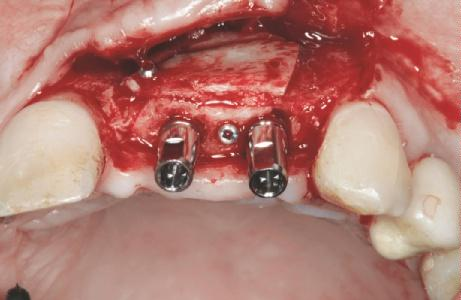
\includegraphics[width=221.1023pt,height=143.7724pt]{latexImage_f582192ab14a99b88cdea732b0e9c069.png}}
\put(58.7009,-449.3404){\fontsize{9}{1}\usefont{T1}{cmr}{m}{n}\selectfont\color{color_112230}Fig 3-2c  Wound closure with 6-0 monofilament resorb-}
\put(58.70092,-460.3384){\fontsize{9}{1}\usefont{T1}{cmr}{m}{n}\selectfont\color{color_72488}able sutures.}
\put(57.65596,-435.3801){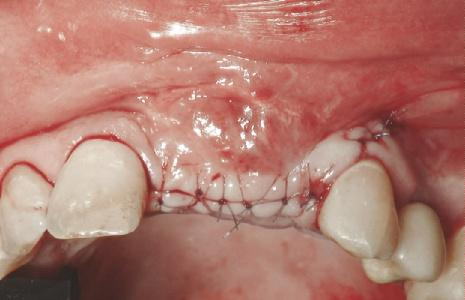
\includegraphics[width=223.2pt,height=143.8152pt]{latexImage_89827327ec3e1176d44a1a06e98513f8.png}}
\put(293.9764,-449.3404){\fontsize{9}{1}\usefont{T1}{cmr}{m}{n}\selectfont\color{color_112230}Fig}
\put(293.9764,-435.3883){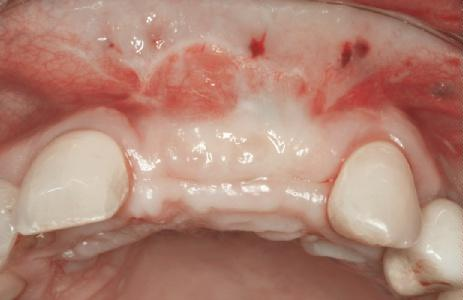
\includegraphics[width=222.1128pt,height=143.7912pt]{latexImage_78fdb88e7eb9490ee2eda6fef96cb240.png}}
\end{picture}
\newpage
\begin{tikzpicture}[overlay]\path(0pt,0pt);\end{tikzpicture}
\begin{picture}(-5,0)(2.5,0)
\put(493.133,-754.1789){\fontsize{11}{1}\usefont{T1}{cmr}{m}{n}\selectfont\color{color_112230}85}
\put(255.698,-29.88385){\fontsize{11}{1}\usefont{T1}{cmr}{m}{n}\selectfont\color{color_112230}3.4}
\put(272.825,-29.88391){\fontsize{11}{1}\usefont{T1}{cmr}{m}{n}\selectfont\color{color_112230} Soft tissue management before augmentation}
\put(50.1969,-300.7559){\fontsize{10.8}{1}\usefont{T1}{cmr}{m}{n}\selectfont\color{color_72488}sign is best. Larger raspatories can only be }
\put(50.1969,-315.7571){\fontsize{10.8}{1}\usefont{T1}{cmr}{m}{n}\selectfont\color{color_72488}used for the atraumatic lifting of flaps. There }
\put(50.1969,-330.7583){\fontsize{10.8}{1}\usefont{T1}{cmr}{m}{n}\selectfont\color{color_72488}should be at least one anatomical and one sur}
\put(267.7024,-330.7561){\fontsize{10.8}{1}\usefont{T1}{cmr}{m}{n}\selectfont\color{color_72488}-}
\put(50.19691,-345.7563){\fontsize{10.8}{1}\usefont{T1}{cmr}{m}{n}\selectfont\color{color_72488}gical forceps, the latter specifically designed }
\put(50.19691,-360.7574){\fontsize{10.8}{1}\usefont{T1}{cmr}{m}{n}\selectfont\color{color_72488}for microsurgery. Without lip and muscle re}
\put(267.7024,-360.7564){\fontsize{10.8}{1}\usefont{T1}{cmr}{m}{n}\selectfont\color{color_72488}-}
\put(50.19691,-375.7565){\fontsize{10.8}{1}\usefont{T1}{cmr}{m}{n}\selectfont\color{color_72488}traction, a delicate flap, or a free or pedicle }
\put(50.19691,-390.7577){\fontsize{10.8}{1}\usefont{T1}{cmr}{m}{n}\selectfont\color{color_72488}connective tissue graft, can be optimally held }
\put(50.19691,-405.7589){\fontsize{10.8}{1}\usefont{T1}{cmr}{m}{n}\selectfont\color{color_72488}using a surgical Cooley forceps without much }
\put(50.19691,-420.7601){\fontsize{10.8}{1}\usefont{T1}{cmr}{m}{n}\selectfont\color{color_72488}pressure. If too much pressure is applied in the }
\put(50.19691,-435.7613){\fontsize{10.8}{1}\usefont{T1}{cmr}{m}{n}\selectfont\color{color_72488}case of anatomical forceps, the delicate flap }
\put(50.19691,-450.7625){\fontsize{10.8}{1}\usefont{T1}{cmr}{m}{n}\selectfont\color{color_72488}can be significantly traumatized or bruised. In }
\put(50.19691,-465.7636){\fontsize{10.8}{1}\usefont{T1}{cmr}{m}{n}\selectfont\color{color_72488}the case of very thin flaps or free mucosal }
\put(50.19691,-480.7648){\fontsize{10.8}{1}\usefont{T1}{cmr}{m}{n}\selectfont\color{color_72488}grafts, an anatomical forceps is the best choice }
\put(50.19691,-495.766){\fontsize{10.8}{1}\usefont{T1}{cmr}{m}{n}\selectfont\color{color_72488}for atraumatic handling without the risk of per}
\put(267.7024,-495.7563){\fontsize{10.8}{1}\usefont{T1}{cmr}{m}{n}\selectfont\color{color_72488}-}
\put(50.19691,-510.7564){\fontsize{10.8}{1}\usefont{T1}{cmr}{m}{n}\selectfont\color{color_72488}foration. For knotting suture threads, either an }
\put(50.19691,-525.7576){\fontsize{10.8}{1}\usefont{T1}{cmr}{m}{n}\selectfont\color{color_72488}anatomical or a surgical forceps with plateau is }
\put(50.19691,-540.7588){\fontsize{10.8}{1}\usefont{T1}{cmr}{m}{n}\selectfont\color{color_72488}suitable to avoid any damage to the suture ma}
\put(267.7024,-540.7566){\fontsize{10.8}{1}\usefont{T1}{cmr}{m}{n}\selectfont\color{color_72488}-}
\put(50.19691,-555.7567){\fontsize{10.8}{1}\usefont{T1}{cmr}{m}{n}\selectfont\color{color_72488}terials when grabbing them. As regards the }
\put(50.19691,-570.7579){\fontsize{10.8}{1}\usefont{T1}{cmr}{m}{n}\selectfont\color{color_72488}choice of needle holder, in addition to the nee}
\put(267.7024,-570.7568){\fontsize{10.8}{1}\usefont{T1}{cmr}{m}{n}\selectfont\color{color_72488}-}
\put(50.19691,-585.757){\fontsize{10.8}{1}\usefont{T1}{cmr}{m}{n}\selectfont\color{color_72488}dle size to be used, the level of experience and }
\put(50.19691,-600.7582){\fontsize{10.8}{1}\usefont{T1}{cmr}{m}{n}\selectfont\color{color_72488}the preference of the surgeon play a decisive }
\put(50.19691,-615.7594){\fontsize{10.8}{1}\usefont{T1}{cmr}{m}{n}\selectfont\color{color_72488}role. Various sizes of the required shape as well }
\put(50.19691,-630.7606){\fontsize{10.8}{1}\usefont{T1}{cmr}{m}{n}\selectfont\color{color_72488}as a slender design are needed to ensure ap}
\put(267.7024,-630.7574){\fontsize{10.8}{1}\usefont{T1}{cmr}{m}{n}\selectfont\color{color_72488}-}
\put(50.19691,-645.7575){\fontsize{10.8}{1}\usefont{T1}{cmr}{m}{n}\selectfont\color{color_72488}propriate access to the interdental areas. Mi-}
\put(50.19691,-660.7576){\fontsize{10.8}{1}\usefont{T1}{cmr}{m}{n}\selectfont\color{color_72488}crosurgical needle holders are usually not }
\put(50.19691,-675.7588){\fontsize{10.8}{1}\usefont{T1}{cmr}{m}{n}\selectfont\color{color_72488}equipped with a lock, although it is of great }
\put(50.19691,-690.76){\fontsize{10.8}{1}\usefont{T1}{cmr}{m}{n}\selectfont\color{color_72488}help in oral and periodontal surgery for con}
\put(267.7024,-690.7579){\fontsize{10.8}{1}\usefont{T1}{cmr}{m}{n}\selectfont\color{color_72488}-}
\put(50.19691,-705.758){\fontsize{10.8}{1}\usefont{T1}{cmr}{m}{n}\selectfont\color{color_72488}trolled rotating movements. The needle holder }
\put(50.19691,-720.7592){\fontsize{10.8}{1}\usefont{T1}{cmr}{m}{n}\selectfont\color{color_72488}by Castroviejo is, for example, equipped with a }
\put(285.4749,-300.758){\fontsize{10.8}{1}\usefont{T1}{cmr}{m}{n}\selectfont\color{color_72488}gentle locking mechanism. In the case of micro }
\put(285.4749,-315.7592){\fontsize{10.8}{1}\usefont{T1}{cmr}{m}{n}\selectfont\color{color_72488}scissors, curved shapes with pointed blades }
\put(285.4749,-330.7603){\fontsize{10.8}{1}\usefont{T1}{cmr}{m}{n}\selectfont\color{color_72488}have proven to be practical.}
\put(299.6445,-345.7615){\fontsize{10.8}{1}\usefont{T1}{cmr}{m}{n}\selectfont\color{color_72488}Some special instruments, e.g. the multi-po}
\put(502.9783,-345.7583){\fontsize{10.8}{1}\usefont{T1}{cmr}{m}{n}\selectfont\color{color_72488}-}
\put(285.4727,-360.7584){\fontsize{10.8}{1}\usefont{T1}{cmr}{m}{n}\selectfont\color{color_72488}sitioned angulated scalpel, can be very useful }
\put(285.4727,-375.7596){\fontsize{10.8}{1}\usefont{T1}{cmr}{m}{n}\selectfont\color{color_72488}to gain access to different intraoral areas for }
\put(285.4727,-390.7608){\fontsize{10.8}{1}\usefont{T1}{cmr}{m}{n}\selectfont\color{color_72488}specific surgeries (Fig}
\put(387.5325,-390.7583){\fontsize{10.8}{1}\usefont{T1}{cmr}{m}{n}\selectfont\color{color_72488} 3-3a and b).}
\put(285.4725,-439.737){\fontsize{14}{1}\usefont{T1}{cmr}{m}{n}\selectfont\color{color_112230}3.4 Soft tissue management before }
\put(325.1625,-456.537){\fontsize{14}{1}\usefont{T1}{cmr}{m}{n}\selectfont\color{color_112230}augmentation}
\put(285.4725,-480.7559){\fontsize{10.8}{1}\usefont{T1}{cmr}{m}{n}\selectfont\color{color_72488}Inflammatory processes and tooth extractions }
\put(285.4725,-495.7571){\fontsize{10.8}{1}\usefont{T1}{cmr}{m}{n}\selectfont\color{color_72488}sometimes lead to pronounced damage to both }
\put(285.4725,-510.7583){\fontsize{10.8}{1}\usefont{T1}{cmr}{m}{n}\selectfont\color{color_72488}hard and soft tissue. In particular, the quantity }
\put(285.4725,-525.7595){\fontsize{10.8}{1}\usefont{T1}{cmr}{m}{n}\selectfont\color{color_72488}and quality of soft tissue, including its regener}
\put(502.978,-525.7562){\fontsize{10.8}{1}\usefont{T1}{cmr}{m}{n}\selectfont\color{color_72488}-}
\put(285.4725,-540.7563){\fontsize{10.8}{1}\usefont{T1}{cmr}{m}{n}\selectfont\color{color_72488}ative characteristics, are severely compromised }
\put(285.4725,-555.7576){\fontsize{10.8}{1}\usefont{T1}{cmr}{m}{n}\selectfont\color{color_72488}in cases involving infected biomaterials or failed }
\put(285.4725,-570.7588){\fontsize{10.8}{1}\usefont{T1}{cmr}{m}{n}\selectfont\color{color_72488}implantation attempts with multiple previous }
\put(285.4725,-585.76){\fontsize{10.8}{1}\usefont{T1}{cmr}{m}{n}\selectfont\color{color_72488}surgeries. It can be an advantage in all these }
\put(285.4725,-600.7612){\fontsize{10.8}{1}\usefont{T1}{cmr}{m}{n}\selectfont\color{color_72488}situations to improve the quality of soft tissue in }
\put(285.4725,-615.7624){\fontsize{10.8}{1}\usefont{T1}{cmr}{m}{n}\selectfont\color{color_72488}this region before actual augmentative mea}
\put(502.978,-615.7559){\fontsize{10.8}{1}\usefont{T1}{cmr}{m}{n}\selectfont\color{color_72488}-}
\put(285.4725,-630.756){\fontsize{10.8}{1}\usefont{T1}{cmr}{m}{n}\selectfont\color{color_72488}sures. This allows for an easier and safer clo-}
\put(285.4725,-645.7562){\fontsize{10.8}{1}\usefont{T1}{cmr}{m}{n}\selectfont\color{color_72488}sure, primarily in relation to vertical bone aug-}
\put(285.4725,-660.7563){\fontsize{10.8}{1}\usefont{T1}{cmr}{m}{n}\selectfont\color{color_72488}mentations. Soft tissue improvement is most }
\put(285.4725,-675.7574){\fontsize{10.8}{1}\usefont{T1}{cmr}{m}{n}\selectfont\color{color_72488}frequently indicated in patients with a thin gin}
\put(502.978,-675.7564){\fontsize{10.8}{1}\usefont{T1}{cmr}{m}{n}\selectfont\color{color_72488}-}
\put(285.4725,-690.7565){\fontsize{10.8}{1}\usefont{T1}{cmr}{m}{n}\selectfont\color{color_72488}gival biotype, as the improved soft tissue has a }
\put(285.4725,-705.7577){\fontsize{10.8}{1}\usefont{T1}{cmr}{m}{n}\selectfont\color{color_72488}protective effect on the hard tissue graft and }
\put(285.4725,-720.7589){\fontsize{10.8}{1}\usefont{T1}{cmr}{m}{n}\selectfont\color{color_72488}ensures a better long-term esthetic result.}
\put(50.1969,-222.8522){\fontsize{9}{1}\usefont{T1}{cmr}{m}{n}\selectfont\color{color_112230}Fig 3-3a  Angulated scalpel for better access from the }
\put(50.1969,-233.8502){\fontsize{9}{1}\usefont{T1}{cmr}{m}{n}\selectfont\color{color_72488}palatal side.}
\put(49.19282,-208.941){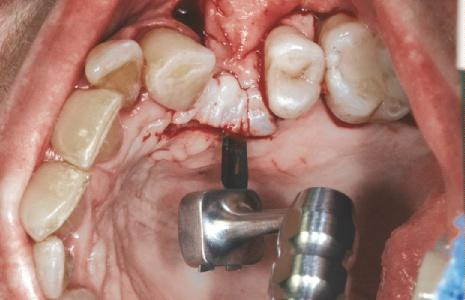
\includegraphics[width=223.1664pt,height=143.9136pt]{latexImage_602bb5aada361ffb0a46220ca0e5da0b.png}}
\put(285.4724,-222.8522){\fontsize{9}{1}\usefont{T1}{cmr}{m}{n}\selectfont\color{color_112230}Fig 3-3b  A supraperiosteal flap preparation in the poster-}
\put(285.4724,-233.8502){\fontsize{9}{1}\usefont{T1}{cmr}{m}{n}\selectfont\color{color_72488}ior maxilla is made easier using an angulated scalpel.}
\put(285.4725,-208.9407){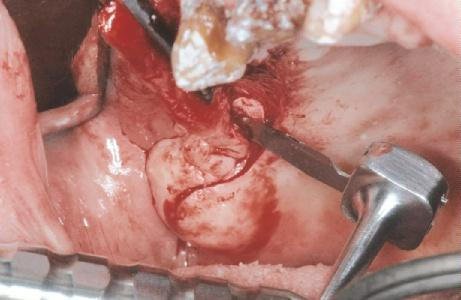
\includegraphics[width=221.1024pt,height=143.8618pt]{latexImage_c5670f72312ffbafd56cc56dff000dae.png}}
\end{picture}
\newpage
\begin{tikzpicture}[overlay]\path(0pt,0pt);\end{tikzpicture}
\begin{picture}(-5,0)(2.5,0)
\put(58.7009,-754.1789){\fontsize{11}{1}\usefont{T1}{cmr}{m}{n}\selectfont\color{color_112230}86}
\put(58.7009,-29.88385){\fontsize{11}{1}\usefont{T1}{cmr}{m}{n}\selectfont\color{color_112230}3}
\put(64.9269,-29.88391){\fontsize{11}{1}\usefont{T1}{cmr}{m}{n}\selectfont\color{color_112230} Soft tissue management and bone augmentation in implantology}
\put(308.1496,-555.7559){\fontsize{10.8}{1}\usefont{T1}{cmr}{m}{n}\selectfont\color{color_72488}A thin biotype is easily diagnosed by prob-}
\put(293.9768,-570.756){\fontsize{10.8}{1}\usefont{T1}{cmr}{m}{n}\selectfont\color{color_72488}ing, as the periodontal probe is visible through }
\put(293.9768,-585.7573){\fontsize{10.8}{1}\usefont{T1}{cmr}{m}{n}\selectfont\color{color_72488}the tissue, and it is a predisposing factor for the }
\put(293.9768,-600.7584){\fontsize{10.8}{1}\usefont{T1}{cmr}{m}{n}\selectfont\color{color_72488}formation of recessions. It may therefore be rea}
\put(511.4823,-600.7563){\fontsize{10.8}{1}\usefont{T1}{cmr}{m}{n}\selectfont\color{color_72488}-}
\put(293.9768,-615.7564){\fontsize{10.8}{1}\usefont{T1}{cmr}{m}{n}\selectfont\color{color_72488}sonable to change biotypes from thin to thick, }
\put(293.9768,-630.7576){\fontsize{10.8}{1}\usefont{T1}{cmr}{m}{n}\selectfont\color{color_72488}with consideration of esthetics. This can be }
\put(293.9768,-645.7588){\fontsize{10.8}{1}\usefont{T1}{cmr}{m}{n}\selectfont\color{color_72488}achieved by both free gingival and connective }
\put(293.9768,-660.76){\fontsize{10.8}{1}\usefont{T1}{cmr}{m}{n}\selectfont\color{color_72488}tissue grafts and palatal pedicle connective tis}
\put(511.4823,-660.7568){\fontsize{10.8}{1}\usefont{T1}{cmr}{m}{n}\selectfont\color{color_72488}-}
\put(293.9768,-675.7569){\fontsize{10.8}{1}\usefont{T1}{cmr}{m}{n}\selectfont\color{color_72488}sue flaps (Fig}
\put(358.0204,-675.7559){\fontsize{10.8}{1}\usefont{T1}{cmr}{m}{n}\selectfont\color{color_72488} 3-4a to l). Rotation flaps can be }
\put(293.9764,-690.7571){\fontsize{10.8}{1}\usefont{T1}{cmr}{m}{n}\selectfont\color{color_72488}created, epithelialized or deepithelialized from }
\put(293.9764,-705.7583){\fontsize{10.8}{1}\usefont{T1}{cmr}{m}{n}\selectfont\color{color_72488}buccal mucosa or the palate. The volume and }
\put(293.9764,-720.7595){\fontsize{10.8}{1}\usefont{T1}{cmr}{m}{n}\selectfont\color{color_72488}quality of the soft tissue can also be improved }
\put(58.7009,-222.8522){\fontsize{9}{1}\usefont{T1}{cmr}{m}{n}\selectfont\color{color_112230}Fig 3-4a  Poor esthetic situation after looseness of an }
\put(58.7009,-233.8502){\fontsize{9}{1}\usefont{T1}{cmr}{m}{n}\selectfont\color{color_72488}implant at the position of the first left central incisor, and }
\put(58.7009,-244.8482){\fontsize{9}{1}\usefont{T1}{cmr}{m}{n}\selectfont\color{color_72488}bone and soft tissue loss on the implant at the position of }
\put(58.7009,-255.8462){\fontsize{9}{1}\usefont{T1}{cmr}{m}{n}\selectfont\color{color_72488}the lateral incisor}
\put(58.70083,-208.8704){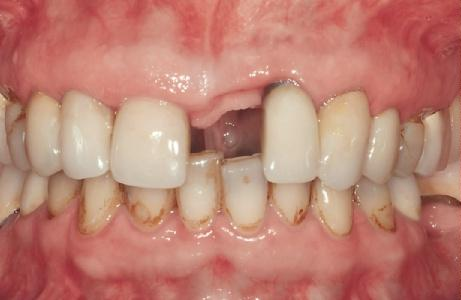
\includegraphics[width=221.1023pt,height=143.7724pt]{latexImage_034e13434f3fd21e36708c24c6807ca4.png}}
\put(293.9764,-222.8522){\fontsize{9}{1}\usefont{T1}{cmr}{m}{n}\selectfont\color{color_112230}Fig 3-4b  After removal of the crown, explantation of the }
\put(293.9764,-233.8502){\fontsize{9}{1}\usefont{T1}{cmr}{m}{n}\selectfont\color{color_72488}implant using the BTI explantation system (BTI, Vito-}
\put(293.9764,-244.8482){\fontsize{9}{1}\usefont{T1}{cmr}{m}{n}\selectfont\color{color_72488}ria-Gasteiz, Spain).}
\put(293.9764,-207.8503){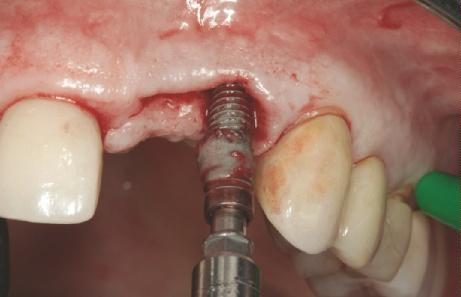
\includegraphics[width=221.1023pt,height=142.7487pt]{latexImage_8aefa99a4fce8f1310dd95421ae27876.png}}
\put(58.7008,-481.8631){\fontsize{9}{1}\usefont{T1}{cmr}{m}{n}\selectfont\color{color_112230}Fig 3-4c  Preparation of a pedicle }
\put(58.70081,-492.8611){\fontsize{9}{1}\usefont{T1}{cmr}{m}{n}\selectfont\color{color_72488}connective tissue flap in the left }
\put(58.70081,-503.8591){\fontsize{9}{1}\usefont{T1}{cmr}{m}{n}\selectfont\color{color_72488}palate.}
\put(57.68747,-466.8613){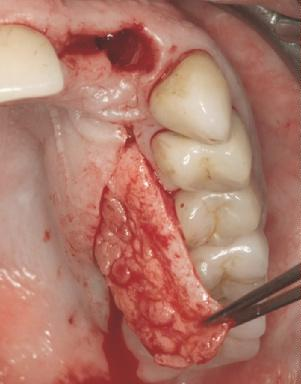
\includegraphics[width=144.7029pt,height=184.252pt]{latexImage_d0e5f9f711d08999d0b76b2fe8fc77f0.png}}
\put(215.5517,-481.8631){\fontsize{9}{1}\usefont{T1}{cmr}{m}{n}\selectfont\color{color_112230}Fig 3-4d  The pedicle connective }
\put(215.5517,-492.8611){\fontsize{9}{1}\usefont{T1}{cmr}{m}{n}\selectfont\color{color_72488}tissue flap is tunneled under a soft }
\put(215.5517,-503.8591){\fontsize{9}{1}\usefont{T1}{cmr}{m}{n}\selectfont\color{color_72488}tissue bridge to cover the defect and }
\put(215.5517,-514.8571){\fontsize{9}{1}\usefont{T1}{cmr}{m}{n}\selectfont\color{color_72488}improve the quality of the soft tissue.}
\put(214.6126,-466.8613){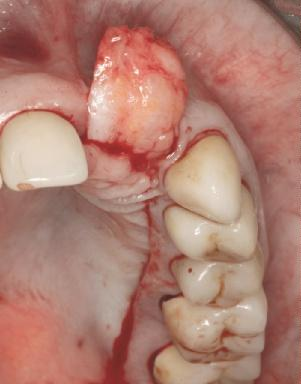
\includegraphics[width=144.5543pt,height=184.2519pt]{latexImage_27030b08e32c9991983087c971239423.png}}
\put(372.4025,-481.8631){\fontsize{9}{1}\usefont{T1}{cmr}{m}{n}\selectfont\color{color_112230}Fig 3-4e  Wound closure with 6-0 }
\put(372.4025,-492.8611){\fontsize{9}{1}\usefont{T1}{cmr}{m}{n}\selectfont\color{color_72488}sutures without any releasing }
\put(372.4025,-503.8591){\fontsize{9}{1}\usefont{T1}{cmr}{m}{n}\selectfont\color{color_72488}incision.}
\put(371.3602,-466.8613){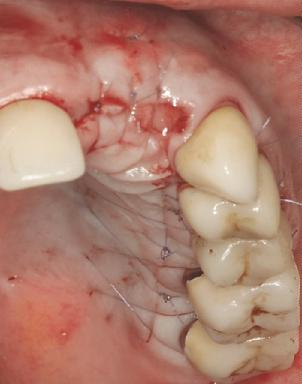
\includegraphics[width=144.7551pt,height=184.252pt]{latexImage_6e171dfb4b09149d4ec2d3ac7d90d391.png}}
\put(58.7008,-698.8504){\fontsize{9}{1}\usefont{T1}{cmr}{m}{n}\selectfont\color{color_112230}Fig}
\put(58.70083,-684.8776){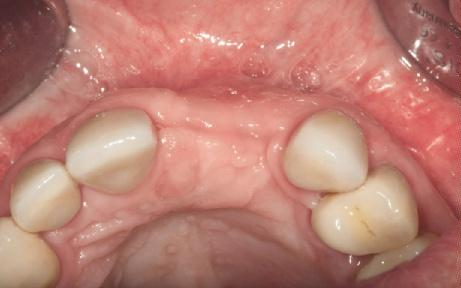
\includegraphics[width=221.1023pt,height=138.1153pt]{latexImage_ee84690f7254a91a26cc4eac318344cc.png}}
\end{picture}
\newpage
\begin{tikzpicture}[overlay]\path(0pt,0pt);\end{tikzpicture}
\begin{picture}(-5,0)(2.5,0)
\put(493.133,-754.1789){\fontsize{11}{1}\usefont{T1}{cmr}{m}{n}\selectfont\color{color_112230}87}
\put(255.698,-29.88385){\fontsize{11}{1}\usefont{T1}{cmr}{m}{n}\selectfont\color{color_112230}3.4}
\put(272.825,-29.88391){\fontsize{11}{1}\usefont{T1}{cmr}{m}{n}\selectfont\color{color_112230} Soft tissue management before augmentation}
\put(50.1969,-222.8522){\fontsize{9}{1}\usefont{T1}{cmr}{m}{n}\selectfont\color{color_112230}Fig}
\put(50.19689,-208.8703){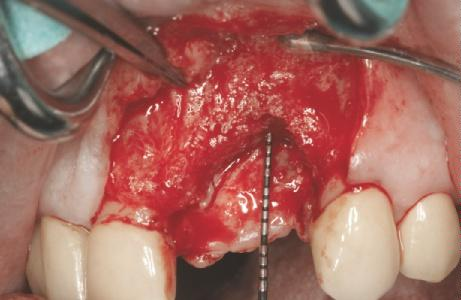
\includegraphics[width=221.1023pt,height=143.7724pt]{latexImage_ba5b927119c90e02d92544080a3f13d2.png}}
\put(285.4724,-222.8522){\fontsize{9}{1}\usefont{T1}{cmr}{m}{n}\selectfont\color{color_112230}Fig 3-4h  Vertical bone augmentation with bone grafts }
\put(285.4724,-233.8502){\fontsize{9}{1}\usefont{T1}{cmr}{m}{n}\selectfont\color{color_72488}from the left mandibular retromolar area following the pro-}
\put(285.4724,-244.8482){\fontsize{9}{1}\usefont{T1}{cmr}{m}{n}\selectfont\color{color_72488}tocol of the SBB technique.}
\put(285.4725,-208.8703){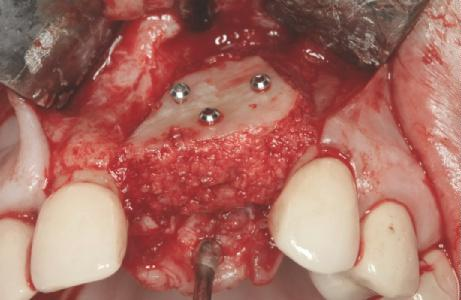
\includegraphics[width=221.1023pt,height=143.7724pt]{latexImage_741b620070afc950d27553af428e7bd5.png}}
\put(50.1969,-439.3434){\fontsize{9}{1}\usefont{T1}{cmr}{m}{n}\selectfont\color{color_112230}Fig 3-4i  Closure of the wound with 6-0 monofilament }
\put(50.1969,-450.3414){\fontsize{9}{1}\usefont{T1}{cmr}{m}{n}\selectfont\color{color_72488}sutures (only one releasing incision was necessary for the }
\put(50.1969,-461.3394){\fontsize{9}{1}\usefont{T1}{cmr}{m}{n}\selectfont\color{color_72488}wound closure).}
\put(50.19691,-425.3615){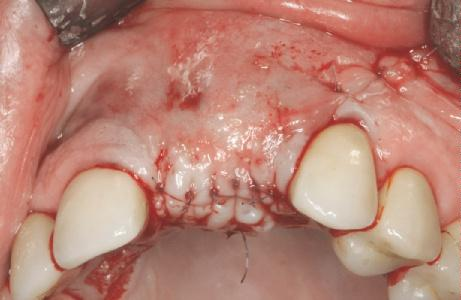
\includegraphics[width=221.1023pt,height=143.7724pt]{latexImage_c540338a6b36f36c39a4c046e48770b8.png}}
\put(50.1969,-698.8504){\fontsize{9}{1}\usefont{T1}{cmr}{m}{n}\selectfont\color{color_112230}Fig 3-4k  Bone exposure using the same incision line }
\put(50.1969,-709.8484){\fontsize{9}{1}\usefont{T1}{cmr}{m}{n}\selectfont\color{color_72488}made during the grafting procedure: insertion of two im-}
\put(50.19691,-720.8464){\fontsize{9}{1}\usefont{T1}{cmr}{m}{n}\selectfont\color{color_72488}plants in the grafted area.}
\put(50.1969,-683.8486){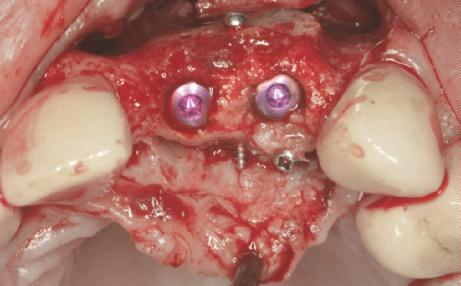
\includegraphics[width=221.1024pt,height=137.0966pt]{latexImage_1b89ed258bfc83aaa3ff4d08854c0ab8.png}}
\put(285.4724,-698.8504){\fontsize{9}{1}\usefont{T1}{cmr}{m}{n}\selectfont\color{color_112230}Fig}
\put(285.4724,-684.8775){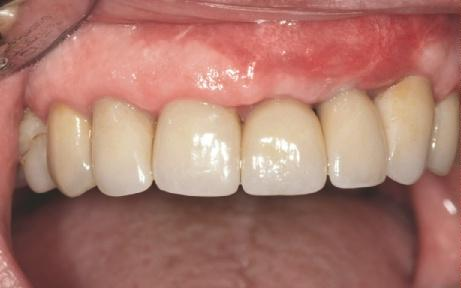
\includegraphics[width=221.1023pt,height=138.1398pt]{latexImage_6be2feed2fbb03ef7afe8307942447dc.png}}
\put(285.4724,-439.3434){\fontsize{9}{1}\usefont{T1}{cmr}{m}{n}\selectfont\color{color_112230}Fig}
\put(285.4725,-425.373){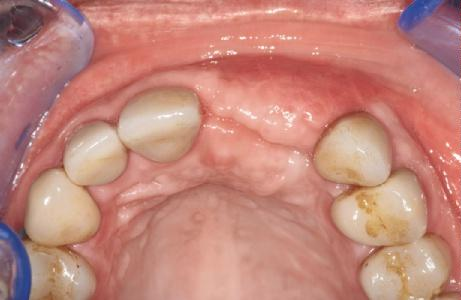
\includegraphics[width=221.1023pt,height=143.7952pt]{latexImage_5b3b4312e361a0715892f12d3b058a4c.png}}
\end{picture}
\newpage
\begin{tikzpicture}[overlay]\path(0pt,0pt);\end{tikzpicture}
\begin{picture}(-5,0)(2.5,0)
\put(58.7009,-754.1789){\fontsize{11}{1}\usefont{T1}{cmr}{m}{n}\selectfont\color{color_112230}88}
\put(58.7009,-29.88385){\fontsize{11}{1}\usefont{T1}{cmr}{m}{n}\selectfont\color{color_112230}3}
\put(64.9269,-29.88391){\fontsize{11}{1}\usefont{T1}{cmr}{m}{n}\selectfont\color{color_112230} Soft tissue management and bone augmentation in implantology}
\put(58.7008,-495.7559){\fontsize{10.8}{1}\usefont{T1}{cmr}{m}{n}\selectfont\color{color_72488}through free gingival and/or connective tissue }
\put(58.7008,-510.7571){\fontsize{10.8}{1}\usefont{T1}{cmr}{m}{n}\selectfont\color{color_72488}grafts, which can at the same time counteract }
\put(58.7008,-525.7583){\fontsize{10.8}{1}\usefont{T1}{cmr}{m}{n}\selectfont\color{color_72488}shifts in the mucogingival junction.}
\put(58.7008,-567.9331){\fontsize{12.5}{1}\usefont{T1}{cmr}{m}{n}\selectfont\color{color_112230}3.4.1 Incisions before augmentation}
\put(58.7008,-585.7559){\fontsize{10.8}{1}\usefont{T1}{cmr}{m}{n}\selectfont\color{color_72488}From the very beginning, the adequacy of the }
\put(58.7008,-600.7571){\fontsize{10.8}{1}\usefont{T1}{cmr}{m}{n}\selectfont\color{color_72488}cuts has great significance for the later esthetic }
\put(58.7008,-615.7583){\fontsize{10.8}{1}\usefont{T1}{cmr}{m}{n}\selectfont\color{color_72488}success. If the existing tissue is thin, it is rec}
\put(276.2074,-615.7562){\fontsize{10.8}{1}\usefont{T1}{cmr}{m}{n}\selectfont\color{color_72488}-}
\put(58.7008,-630.7563){\fontsize{10.8}{1}\usefont{T1}{cmr}{m}{n}\selectfont\color{color_72488}ommended to place the incision strictly vertical-}
\put(58.7008,-645.7564){\fontsize{10.8}{1}\usefont{T1}{cmr}{m}{n}\selectfont\color{color_72488}ly in order to achieve two equally thick flap mar-}
\put(58.7008,-660.7565){\fontsize{10.8}{1}\usefont{T1}{cmr}{m}{n}\selectfont\color{color_72488}gins and thereby optimize suture closure, }
\put(58.7008,-675.7577){\fontsize{10.8}{1}\usefont{T1}{cmr}{m}{n}\selectfont\color{color_72488}healing, and the final results. Independent of }
\put(58.7008,-690.7589){\fontsize{10.8}{1}\usefont{T1}{cmr}{m}{n}\selectfont\color{color_72488}the phase of soft tissue management, the inci}
\put(276.2074,-690.7568){\fontsize{10.8}{1}\usefont{T1}{cmr}{m}{n}\selectfont\color{color_72488}-}
\put(58.7008,-705.7569){\fontsize{10.8}{1}\usefont{T1}{cmr}{m}{n}\selectfont\color{color_72488}sion should ensure the necessary accessibility of }
\put(58.7008,-720.7581){\fontsize{10.8}{1}\usefont{T1}{cmr}{m}{n}\selectfont\color{color_72488}the operation site and offer the required mobili}
\put(276.2074,-720.757){\fontsize{10.8}{1}\usefont{T1}{cmr}{m}{n}\selectfont\color{color_72488}-}
\put(58.7009,-420.0569){\fontsize{9}{1}\usefont{T1}{cmr}{m}{n}\selectfont\color{color_112230}Fig 3-5c  Connective tissue graft harvested from the pal-}
\put(58.70089,-431.0549){\fontsize{9}{1}\usefont{T1}{cmr}{m}{n}\selectfont\color{color_72488}ate for the soft tissue augmentation.}
\put(58.7009,-406.0751){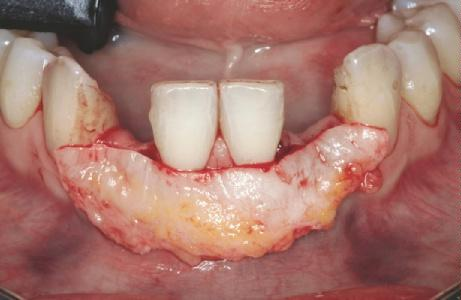
\includegraphics[width=221.1023pt,height=143.7724pt]{latexImage_303b5372914bf742ff594ef9a46ec325.png}}
\put(293.9764,-420.0569){\fontsize{9}{1}\usefont{T1}{cmr}{m}{n}\selectfont\color{color_112230}Fig 3-5d  The connective tissue graft is placed under the }
\put(293.9764,-431.0549){\fontsize{9}{1}\usefont{T1}{cmr}{m}{n}\selectfont\color{color_72488}tunneled mucosa and stabilized with 6-0 sutures at the }
\put(293.9764,-442.0529){\fontsize{9}{1}\usefont{T1}{cmr}{m}{n}\selectfont\color{color_72488}area of the lateral incisors.}
\put(293.9765,-405.0551){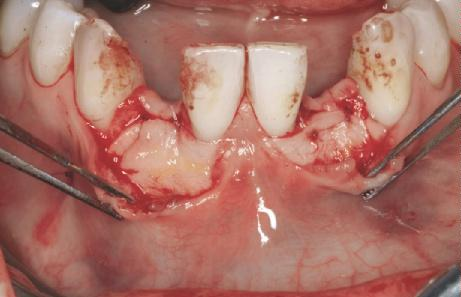
\includegraphics[width=221.1023pt,height=142.7487pt]{latexImage_3b2299bd7c011b1111e951df36d0faa6.png}}
\put(58.7009,-222.8522){\fontsize{9}{1}\usefont{T1}{cmr}{m}{n}\selectfont\color{color_112230}Fig 3-5a  Soft tissue recession on the two mandibular }
\put(58.7009,-233.8502){\fontsize{9}{1}\usefont{T1}{cmr}{m}{n}\selectfont\color{color_72488}central incisors and agenesia of the two lateral incisors.}
\put(58.70083,-208.8719){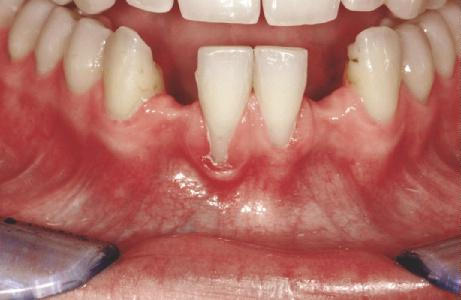
\includegraphics[width=221.1023pt,height=143.7753pt]{latexImage_1c48fcf6d974292c917a01866b11d349.png}}
\put(293.9764,-222.8522){\fontsize{9}{1}\usefont{T1}{cmr}{m}{n}\selectfont\color{color_112230}Fig 3-5b  Preparation of a partial thickness flap on the }
\put(293.9764,-233.8502){\fontsize{9}{1}\usefont{T1}{cmr}{m}{n}\selectfont\color{color_72488}area of the lateral incisors, and tunneling the buccal mu-}
\put(293.9764,-244.8482){\fontsize{9}{1}\usefont{T1}{cmr}{m}{n}\selectfont\color{color_72488}cosa of the central incisors.}
\put(293.9764,-207.8503){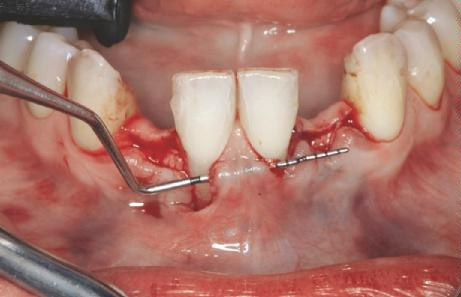
\includegraphics[width=221.1023pt,height=142.7487pt]{latexImage_524cf66bcb8bc6c2e1a75d77a49ad58a.png}}
\put(293.9764,-495.7559){\fontsize{10.8}{1}\usefont{T1}{cmr}{m}{n}\selectfont\color{color_72488}zation opportunities. In the case of sulcular in-}
\put(293.9764,-510.756){\fontsize{10.8}{1}\usefont{T1}{cmr}{m}{n}\selectfont\color{color_72488}cisions, the blade cuts papillae directly under }
\put(293.9764,-525.7572){\fontsize{10.8}{1}\usefont{T1}{cmr}{m}{n}\selectfont\color{color_72488}the tooth contact point, parallel to the tooth }
\put(293.9764,-540.7584){\fontsize{10.8}{1}\usefont{T1}{cmr}{m}{n}\selectfont\color{color_72488}axis, and the whole gingiva is incorporated into }
\put(293.9764,-555.7596){\fontsize{10.8}{1}\usefont{T1}{cmr}{m}{n}\selectfont\color{color_72488}the flap. Releasing incisions in the gingival mar}
\put(511.483,-555.7563){\fontsize{10.8}{1}\usefont{T1}{cmr}{m}{n}\selectfont\color{color_72488}-}
\put(293.9764,-570.7565){\fontsize{10.8}{1}\usefont{T1}{cmr}{m}{n}\selectfont\color{color_72488}gin should be altogether avoided before aug-}
\put(293.9764,-585.7566){\fontsize{10.8}{1}\usefont{T1}{cmr}{m}{n}\selectfont\color{color_72488}mentation; the only exception is in the case of }
\put(293.9764,-600.7578){\fontsize{10.8}{1}\usefont{T1}{cmr}{m}{n}\selectfont\color{color_72488}auxiliary access incisions in the mucosa for the }
\put(293.9764,-615.759){\fontsize{10.8}{1}\usefont{T1}{cmr}{m}{n}\selectfont\color{color_72488}placement of grafts. In the pre-augmentative }
\put(293.9764,-630.7603){\fontsize{10.8}{1}\usefont{T1}{cmr}{m}{n}\selectfont\color{color_72488}phase, only mucosal flaps – also called }
\put(293.9764,-645.7615){\fontsize{10.8}{1}\usefont{T1}{cmr}{m}{n}\selectfont\color{color_72488}split-thickness flaps – should be used (Fig}
\put(490.6228,-645.7607){\fontsize{10.8}{1}\usefont{T1}{cmr}{m}{n}\selectfont\color{color_72488} 3-5a }
\put(293.9764,-660.7619){\fontsize{10.8}{1}\usefont{T1}{cmr}{m}{n}\selectfont\color{color_72488}to o). If a thin layer of connective tissue and }
\put(293.9764,-675.7631){\fontsize{10.8}{1}\usefont{T1}{cmr}{m}{n}\selectfont\color{color_72488}periosteum are left on the bone, grafts heal bet}
\put(511.483,-675.7556){\fontsize{10.8}{1}\usefont{T1}{cmr}{m}{n}\selectfont\color{color_72488}-}
\put(293.9764,-690.7557){\fontsize{10.8}{1}\usefont{T1}{cmr}{m}{n}\selectfont\color{color_72488}ter due to the vascular supply from all sides.}
\put(503.3308,-688.0559){\fontsize{6.48}{1}\usefont{T1}{cmr}{m}{n}\selectfont\color{color_72488}134}
\put(515.0788,-690.7559){\fontsize{10.8}{1}\usefont{T1}{cmr}{m}{n}\selectfont\color{color_72488} }
\put(293.9812,-705.7571){\fontsize{10.8}{1}\usefont{T1}{cmr}{m}{n}\selectfont\color{color_72488}In addition, the resulting bone resorption can be }
\put(293.9812,-720.7583){\fontsize{10.8}{1}\usefont{T1}{cmr}{m}{n}\selectfont\color{color_72488}minimized in the case of a split-thickness flap }
\end{picture}
\newpage
\begin{tikzpicture}[overlay]\path(0pt,0pt);\end{tikzpicture}
\begin{picture}(-5,0)(2.5,0)
\put(493.133,-754.1789){\fontsize{11}{1}\usefont{T1}{cmr}{m}{n}\selectfont\color{color_112230}89}
\put(255.698,-29.88385){\fontsize{11}{1}\usefont{T1}{cmr}{m}{n}\selectfont\color{color_112230}3.4}
\put(272.825,-29.88391){\fontsize{11}{1}\usefont{T1}{cmr}{m}{n}\selectfont\color{color_112230} Soft tissue management before augmentation}
\put(50.1969,-420.0569){\fontsize{9}{1}\usefont{T1}{cmr}{m}{n}\selectfont\color{color_112230}Fig 3-5g  Clinical appearance 6 weeks postoperatively. }
\put(50.20591,-431.0549){\fontsize{9}{1}\usefont{T1}{cmr}{m}{n}\selectfont\color{color_72488}The temporary restoration is performed as a Maryland }
\put(50.20591,-442.0529){\fontsize{9}{1}\usefont{T1}{cmr}{m}{n}\selectfont\color{color_72488}bridge.}
\put(50.19691,-406.0767){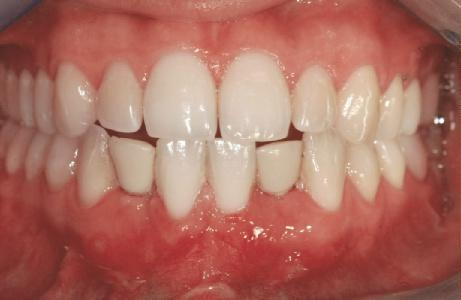
\includegraphics[width=221.1023pt,height=143.7753pt]{latexImage_8f96b0af2dd085a558ced42e9c474c1f.png}}
\put(285.4725,-420.0569){\fontsize{9}{1}\usefont{T1}{cmr}{m}{n}\selectfont\color{color_112230}Fig}
\put(284.5869,-405.0551){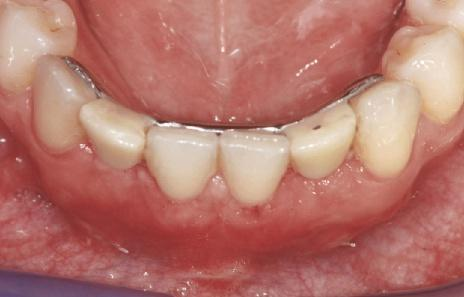
\includegraphics[width=222.8736pt,height=142.7528pt]{latexImage_b44f95744fec30c3501ace9e218ed9c8.png}}
\put(50.1969,-222.8522){\fontsize{9}{1}\usefont{T1}{cmr}{m}{n}\selectfont\color{color_112230}Fig}
\put(50.19688,-208.8703){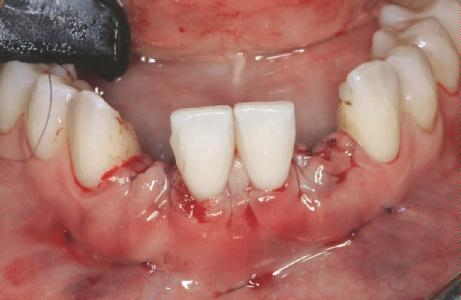
\includegraphics[width=221.1023pt,height=143.7724pt]{latexImage_e30379d44f7f6e3bac017c05fa303dc4.png}}
\put(285.4725,-222.8522){\fontsize{9}{1}\usefont{T1}{cmr}{m}{n}\selectfont\color{color_112230}Fig}
\put(285.4725,-207.8503){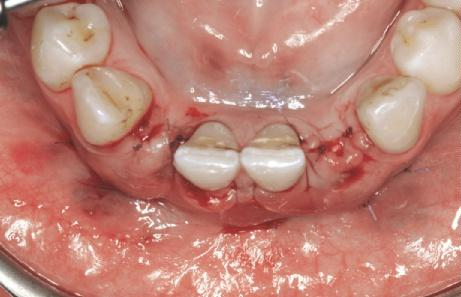
\includegraphics[width=221.1023pt,height=142.7487pt]{latexImage_72235f8b91efded05b502df758a04e0b.png}}
\put(50.1969,-644.9309){\fontsize{9}{1}\usefont{T1}{cmr}{m}{n}\selectfont\color{color_112230}Fig}
\put(50.19689,-630.9492){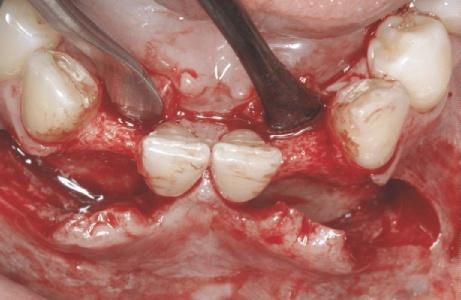
\includegraphics[width=221.1023pt,height=143.7724pt]{latexImage_628ab59352217bbca33684d97fda3668.png}}
\put(285.4724,-644.9309){\fontsize{9}{1}\usefont{T1}{cmr}{m}{n}\selectfont\color{color_112230}Fig}
\put(285.4725,-629.9291){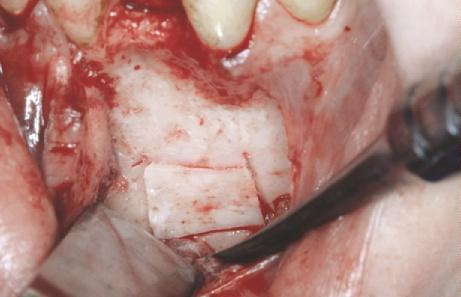
\includegraphics[width=221.1023pt,height=142.7487pt]{latexImage_ae41ed9332e63c4ea6cf0e430753dd4d.png}}
\put(50.1969,-675.7559){\fontsize{10.8}{1}\usefont{T1}{cmr}{m}{n}\selectfont\color{color_72488}dissection, as compared with mucoperiosteal }
\put(50.1969,-690.7571){\fontsize{10.8}{1}\usefont{T1}{cmr}{m}{n}\selectfont\color{color_72488}flaps with denudation of bone.}
\put(188.6632,-688.0559){\fontsize{6.48}{1}\usefont{T1}{cmr}{m}{n}\selectfont\color{color_72488}60,135,166,187}
\put(237.2364,-690.7559){\fontsize{10.8}{1}\usefont{T1}{cmr}{m}{n}\selectfont\color{color_72488} Excep-}
\put(50.19767,-705.756){\fontsize{10.8}{1}\usefont{T1}{cmr}{m}{n}\selectfont\color{color_72488}tions to this concept are situations where the }
\put(50.19767,-720.7572){\fontsize{10.8}{1}\usefont{T1}{cmr}{m}{n}\selectfont\color{color_72488}soft tissue augmentation has to be combined }
\put(285.4756,-675.7536){\fontsize{10.8}{1}\usefont{T1}{cmr}{m}{n}\selectfont\color{color_72488}with the removal of foreign materials (e.g. bio}
\put(502.979,-675.7558){\fontsize{10.8}{1}\usefont{T1}{cmr}{m}{n}\selectfont\color{color_72488}-}
\put(285.4735,-690.7559){\fontsize{10.8}{1}\usefont{T1}{cmr}{m}{n}\selectfont\color{color_72488}materials after infection). In such cases, the flap }
\put(285.4735,-705.7571){\fontsize{10.8}{1}\usefont{T1}{cmr}{m}{n}\selectfont\color{color_72488}preparation must include bone exposure to re}
\put(502.979,-705.756){\fontsize{10.8}{1}\usefont{T1}{cmr}{m}{n}\selectfont\color{color_72488}-}
\put(285.4735,-720.7562){\fontsize{10.8}{1}\usefont{T1}{cmr}{m}{n}\selectfont\color{color_72488}move the foreign materials. }
\end{picture}
\newpage
\begin{tikzpicture}[overlay]\path(0pt,0pt);\end{tikzpicture}
\begin{picture}(-5,0)(2.5,0)
\put(58.7009,-754.1789){\fontsize{11}{1}\usefont{T1}{cmr}{m}{n}\selectfont\color{color_112230}90}
\put(58.7009,-29.88385){\fontsize{11}{1}\usefont{T1}{cmr}{m}{n}\selectfont\color{color_112230}3}
\put(64.9269,-29.88391){\fontsize{11}{1}\usefont{T1}{cmr}{m}{n}\selectfont\color{color_112230} Soft tissue management and bone augmentation in implantology}
\put(58.7009,-417.9467){\fontsize{9}{1}\usefont{T1}{cmr}{m}{n}\selectfont\color{color_112230}Fig}
\put(58.70083,-403.9648){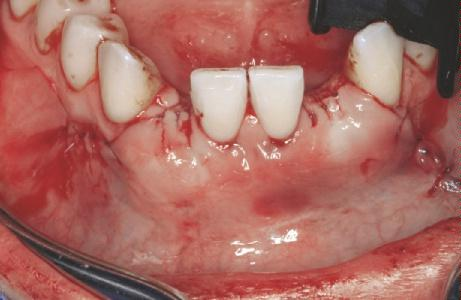
\includegraphics[width=221.1023pt,height=143.7724pt]{latexImage_7e9e955448d2e5be49a7f87bde48ae3d.png}}
\put(293.9764,-417.9467){\fontsize{9}{1}\usefont{T1}{cmr}{m}{n}\selectfont\color{color_112230}Fig 3-5n  After 3 months, implant insertion in the grafted }
\put(293.9764,-428.9447){\fontsize{9}{1}\usefont{T1}{cmr}{m}{n}\selectfont\color{color_72488}bone on the right side.}
\put(293.9765,-402.9448){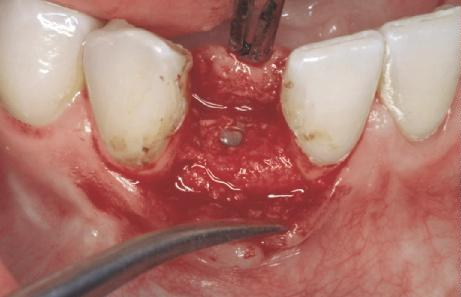
\includegraphics[width=221.1023pt,height=142.7487pt]{latexImage_2626cdf055d04413ac573f37b8ebc8a0.png}}
\put(58.7008,-222.8522){\fontsize{9}{1}\usefont{T1}{cmr}{m}{n}\selectfont\color{color_112230}Fig 3-5k  Bone grafting with simultaneous implant inser-}
\put(58.7008,-233.8502){\fontsize{9}{1}\usefont{T1}{cmr}{m}{n}\selectfont\color{color_72488}tion on the left side.}
\put(58.70083,-208.2574){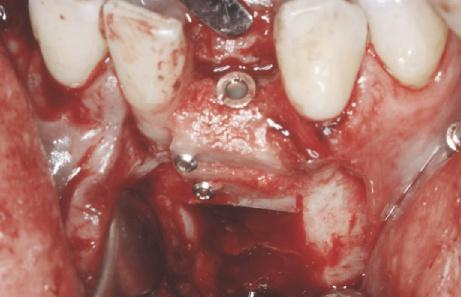
\includegraphics[width=221.1024pt,height=142.5466pt]{latexImage_06665bfe5d40371a2c99e21ac09682ef.png}}
\put(293.9764,-222.8522){\fontsize{9}{1}\usefont{T1}{cmr}{m}{n}\selectfont\color{color_112230}Fig 3-5l  Bone block grafting on the right side. Simultane-}
\put(293.9764,-233.8502){\fontsize{9}{1}\usefont{T1}{cmr}{m}{n}\selectfont\color{color_72488}ous implant placement was not possible here.}
\put(293.9764,-207.8503){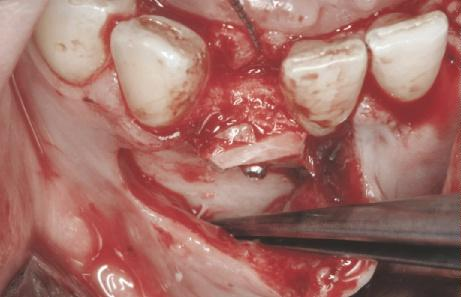
\includegraphics[width=221.1023pt,height=142.7487pt]{latexImage_e5800a2fcc03e9826f68a447bc9633a9.png}}
\put(293.9764,-615.1671){\fontsize{9}{1}\usefont{T1}{cmr}{m}{n}\selectfont\color{color_112230}Fig 3-5o  Definitive restoration performed by the referring }
\put(293.9764,-626.1651){\fontsize{9}{1}\usefont{T1}{cmr}{m}{n}\selectfont\color{color_72488}dentist.}
\put(293.9764,-601.1793){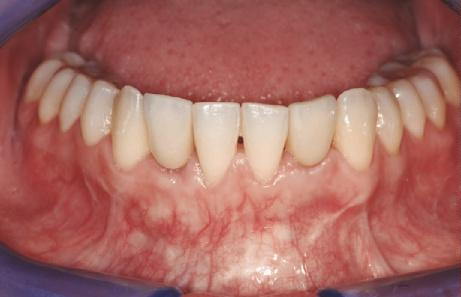
\includegraphics[width=221.1023pt,height=142.7463pt]{latexImage_6bf9a25dfd936cbcd244687e52d0471d.png}}
\put(58.7008,-467.4579){\fontsize{12.5}{1}\usefont{T1}{cmr}{m}{n}\selectfont\color{color_112230}3.4.2 The split-thickness tunnel }
\put(98.3883,-481.9579){\fontsize{12.5}{1}\usefont{T1}{cmr}{m}{n}\selectfont\color{color_112230}technique}
\put(58.7008,-510.7559){\fontsize{10.8}{1}\usefont{T1}{cmr}{m}{n}\selectfont\color{color_72488}Soft tissue thickening is mostly achieved with }
\put(58.7008,-525.7571){\fontsize{10.8}{1}\usefont{T1}{cmr}{m}{n}\selectfont\color{color_72488}connective tissue grafts. The split-thickness }
\put(58.7008,-540.7583){\fontsize{10.8}{1}\usefont{T1}{cmr}{m}{n}\selectfont\color{color_72488}tunnel technique involves the use of free grafts }
\put(58.7008,-555.7595){\fontsize{10.8}{1}\usefont{T1}{cmr}{m}{n}\selectfont\color{color_72488}that restore volume, in particular on the vestib}
\put(276.2074,-555.7562){\fontsize{10.8}{1}\usefont{T1}{cmr}{m}{n}\selectfont\color{color_72488}-}
\put(58.7008,-570.7563){\fontsize{10.8}{1}\usefont{T1}{cmr}{m}{n}\selectfont\color{color_72488}ular aspect of the defect, and therefore com-}
\put(58.7008,-585.7565){\fontsize{10.8}{1}\usefont{T1}{cmr}{m}{n}\selectfont\color{color_72488}pletely exclude the risk of exposure during later }
\put(58.7008,-600.7577){\fontsize{10.8}{1}\usefont{T1}{cmr}{m}{n}\selectfont\color{color_72488}augmentation measures. After the free connec}
\put(276.2074,-600.7566){\fontsize{10.8}{1}\usefont{T1}{cmr}{m}{n}\selectfont\color{color_72488}-}
\put(58.7008,-615.7567){\fontsize{10.8}{1}\usefont{T1}{cmr}{m}{n}\selectfont\color{color_72488}tive tissue graft is harvested from the palate, the }
\put(58.7008,-630.7579){\fontsize{10.8}{1}\usefont{T1}{cmr}{m}{n}\selectfont\color{color_72488}graft bed is opened – beginning with a vertical }
\put(58.7008,-645.7592){\fontsize{10.8}{1}\usefont{T1}{cmr}{m}{n}\selectfont\color{color_72488}mucosal incision – and a Partsch Raspatory or }
\put(58.7008,-660.7604){\fontsize{10.8}{1}\usefont{T1}{cmr}{m}{n}\selectfont\color{color_72488}Kornman scissors are used to bluntly dissect a }
\put(58.7008,-675.7615){\fontsize{10.8}{1}\usefont{T1}{cmr}{m}{n}\selectfont\color{color_72488}tunnel toward the target site. The tunnel is cre}
\put(276.2074,-675.7573){\fontsize{10.8}{1}\usefont{T1}{cmr}{m}{n}\selectfont\color{color_72488}-}
\put(58.7008,-690.7574){\fontsize{10.8}{1}\usefont{T1}{cmr}{m}{n}\selectfont\color{color_72488}ated to be 1.5}
\put(132.5512,-690.7559){\fontsize{10.8}{1}\usefont{T1}{cmr}{m}{n}\selectfont\color{color_72488} times the size of the excised }
\put(58.70079,-705.7571){\fontsize{10.8}{1}\usefont{T1}{cmr}{m}{n}\selectfont\color{color_72488}graft, preserving the anatomical structures as }
\put(58.70079,-720.7583){\fontsize{10.8}{1}\usefont{T1}{cmr}{m}{n}\selectfont\color{color_72488}much as possible (Fig 3-6a to e). The tunnel is }
\put(293.9788,-675.7547){\fontsize{10.8}{1}\usefont{T1}{cmr}{m}{n}\selectfont\color{color_72488}centered on soft tissue deficits and reaches the }
\put(293.9788,-690.7559){\fontsize{10.8}{1}\usefont{T1}{cmr}{m}{n}\selectfont\color{color_72488}keratinized areas of the gingiva, if necessary. If }
\put(293.9788,-705.7571){\fontsize{10.8}{1}\usefont{T1}{cmr}{m}{n}\selectfont\color{color_72488}the keratinized gingiva is very thin, a transition }
\put(293.9788,-720.7583){\fontsize{10.8}{1}\usefont{T1}{cmr}{m}{n}\selectfont\color{color_72488}into a mucoperiosteal flap at the mucogingival }
\end{picture}
\newpage
\begin{tikzpicture}[overlay]\path(0pt,0pt);\end{tikzpicture}
\begin{picture}(-5,0)(2.5,0)
\put(493.133,-754.1789){\fontsize{11}{1}\usefont{T1}{cmr}{m}{n}\selectfont\color{color_112230}91}
\put(255.698,-29.88385){\fontsize{11}{1}\usefont{T1}{cmr}{m}{n}\selectfont\color{color_112230}3.4}
\put(272.825,-29.88391){\fontsize{11}{1}\usefont{T1}{cmr}{m}{n}\selectfont\color{color_112230} Soft tissue management before augmentation}
\put(50.1969,-222.8522){\fontsize{9}{1}\usefont{T1}{cmr}{m}{n}\selectfont\color{color_112230}Fig 3-6a  High bone atrophy in the posterior mandible }
\put(50.1969,-233.8502){\fontsize{9}{1}\usefont{T1}{cmr}{m}{n}\selectfont\color{color_72488}with an extremely thin gingival biotype.}
\put(50.1969,-208.8719){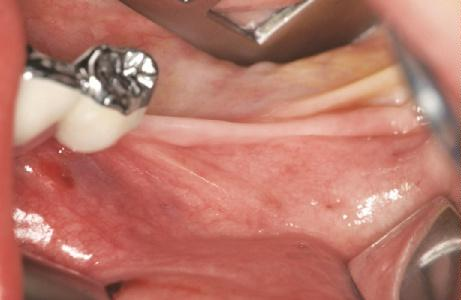
\includegraphics[width=221.1023pt,height=143.7753pt]{latexImage_26530463f2dddadc77eec56cb9cd8bb9.png}}
\put(285.4724,-222.8522){\fontsize{9}{1}\usefont{T1}{cmr}{m}{n}\selectfont\color{color_112230}Fig}
\put(284.413,-207.8503){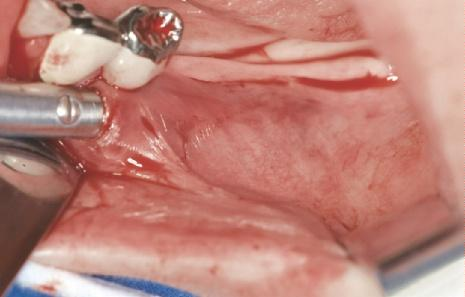
\includegraphics[width=223.2214pt,height=142.7772pt]{latexImage_4aa1aa56b9c0c38a5f1fe39428f49992.png}}
\put(285.4724,-616.3395){\fontsize{9}{1}\usefont{T1}{cmr}{m}{n}\selectfont\color{color_112230}Fig 3-6e  Clinical situation 2 months postoperatively pre-}
\put(285.4724,-627.3375){\fontsize{9}{1}\usefont{T1}{cmr}{m}{n}\selectfont\color{color_72488}senting an improved soft tissue appearance prior to the }
\put(285.4724,-638.3355){\fontsize{9}{1}\usefont{T1}{cmr}{m}{n}\selectfont\color{color_72488}bone grafting.}
\put(285.4725,-601.3376){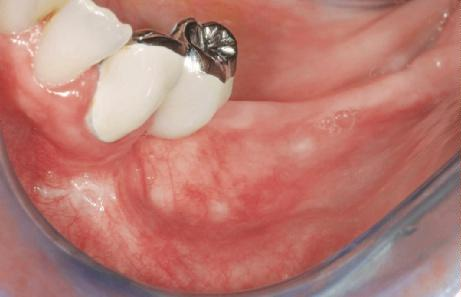
\includegraphics[width=221.1024pt,height=142.7909pt]{latexImage_9936420053f849572b0b887a3edb2a3a.png}}
\put(50.1969,-417.9467){\fontsize{9}{1}\usefont{T1}{cmr}{m}{n}\selectfont\color{color_112230}Fig 3-6c  Connective tissue graft harvested from the pal-}
\put(50.19692,-428.9447){\fontsize{9}{1}\usefont{T1}{cmr}{m}{n}\selectfont\color{color_72488}ate is prepared to be placed through the tunnel.}
\put(50.1969,-403.9664){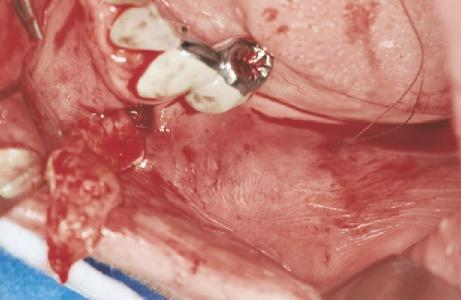
\includegraphics[width=221.1023pt,height=143.7753pt]{latexImage_44080bbb835982dab8a5d702e4b2df6e.png}}
\put(285.4724,-417.9467){\fontsize{9}{1}\usefont{T1}{cmr}{m}{n}\selectfont\color{color_112230}Fig}
\put(284.413,-403.9955){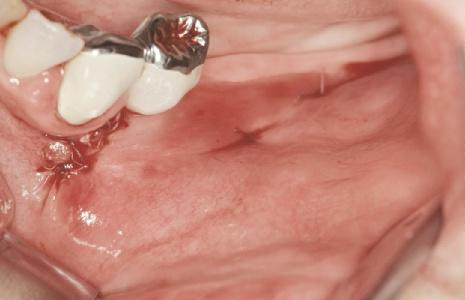
\includegraphics[width=223.2214pt,height=143.8337pt]{latexImage_a56376496533e3bdbdeea2b6bafee404.png}}
\put(50.1969,-465.7559){\fontsize{10.8}{1}\usefont{T1}{cmr}{m}{n}\selectfont\color{color_72488}junction may be necessary to avoid perforations. }
\put(50.1969,-480.7571){\fontsize{10.8}{1}\usefont{T1}{cmr}{m}{n}\selectfont\color{color_72488}The graft is pulled in using a sling suture at the }
\put(50.1969,-495.7583){\fontsize{10.8}{1}\usefont{T1}{cmr}{m}{n}\selectfont\color{color_72488}distal end of the tunnel, which can then be }
\put(50.1969,-510.7595){\fontsize{10.8}{1}\usefont{T1}{cmr}{m}{n}\selectfont\color{color_72488}knotted in the same step to a mattress suture. }
\put(50.1969,-525.7607){\fontsize{10.8}{1}\usefont{T1}{cmr}{m}{n}\selectfont\color{color_72488}The graft should be fixed in the correct position }
\put(50.1969,-540.7618){\fontsize{10.8}{1}\usefont{T1}{cmr}{m}{n}\selectfont\color{color_72488}by at least two mattress sutures, with the use of }
\put(50.1969,-555.7631){\fontsize{10.8}{1}\usefont{T1}{cmr}{m}{n}\selectfont\color{color_72488}a few simple interrupted sutures to prevent rota}
\put(267.7024,-555.7555){\fontsize{10.8}{1}\usefont{T1}{cmr}{m}{n}\selectfont\color{color_72488}-}
\put(50.19691,-570.7556){\fontsize{10.8}{1}\usefont{T1}{cmr}{m}{n}\selectfont\color{color_72488}tion before the vertical access incision can be }
\put(50.19691,-585.7568){\fontsize{10.8}{1}\usefont{T1}{cmr}{m}{n}\selectfont\color{color_72488}closed (Fig}
\put(100.6383,-585.7571){\fontsize{10.8}{1}\usefont{T1}{cmr}{m}{n}\selectfont\color{color_72488} 3-7a to l).}
\put(50.1969,-622.9331){\fontsize{12.5}{1}\usefont{T1}{cmr}{m}{n}\selectfont\color{color_112230}3.4.3 Free connective tissue grafts }
\put(89.88441,-637.4331){\fontsize{12.5}{1}\usefont{T1}{cmr}{m}{n}\selectfont\color{color_112230}before augmentation}
\put(50.1969,-660.7559){\fontsize{10.8}{1}\usefont{T1}{cmr}{m}{n}\selectfont\color{color_72488}Connective tissue grafts are primarily harvested }
\put(50.1969,-675.7571){\fontsize{10.8}{1}\usefont{T1}{cmr}{m}{n}\selectfont\color{color_72488}from the lateral palate, independently of the }
\put(50.1969,-690.7583){\fontsize{10.8}{1}\usefont{T1}{cmr}{m}{n}\selectfont\color{color_72488}phase of soft tissue management. Further donor }
\put(50.1969,-705.7595){\fontsize{10.8}{1}\usefont{T1}{cmr}{m}{n}\selectfont\color{color_72488}sites include the tuber maxillae and the man}
\put(267.7024,-705.7562){\fontsize{10.8}{1}\usefont{T1}{cmr}{m}{n}\selectfont\color{color_72488}-}
\put(50.19691,-720.7563){\fontsize{10.8}{1}\usefont{T1}{cmr}{m}{n}\selectfont\color{color_72488}dibular retromolar region. Free tissue grafts can }
\put(285.4749,-675.7528){\fontsize{10.8}{1}\usefont{T1}{cmr}{m}{n}\selectfont\color{color_72488}be categorized into connective tissue grafts, }
\put(285.4749,-690.754){\fontsize{10.8}{1}\usefont{T1}{cmr}{m}{n}\selectfont\color{color_72488}gingival grafts, and grafts, the last being a com}
\put(502.9783,-690.7562){\fontsize{10.8}{1}\usefont{T1}{cmr}{m}{n}\selectfont\color{color_72488}-}
\put(285.4727,-705.7563){\fontsize{10.8}{1}\usefont{T1}{cmr}{m}{n}\selectfont\color{color_72488}bination of the first two. The ‘lateral palate’ do-}
\put(285.4727,-720.7564){\fontsize{10.8}{1}\usefont{T1}{cmr}{m}{n}\selectfont\color{color_72488}nor site should, however, be further specified, }
\end{picture}
\newpage
\begin{tikzpicture}[overlay]\path(0pt,0pt);\end{tikzpicture}
\begin{picture}(-5,0)(2.5,0)
\put(58.7009,-754.1789){\fontsize{11}{1}\usefont{T1}{cmr}{m}{n}\selectfont\color{color_112230}92}
\put(58.7009,-29.88385){\fontsize{11}{1}\usefont{T1}{cmr}{m}{n}\selectfont\color{color_112230}3}
\put(64.9269,-29.88391){\fontsize{11}{1}\usefont{T1}{cmr}{m}{n}\selectfont\color{color_112230} Soft tissue management and bone augmentation in implantology}
\put(58.7008,-645.7559){\fontsize{10.8}{1}\usefont{T1}{cmr}{m}{n}\selectfont\color{color_72488}as the tissue is thickest in the premolar region }
\put(58.7008,-660.7571){\fontsize{10.8}{1}\usefont{T1}{cmr}{m}{n}\selectfont\color{color_72488}of the palate. Depending on the patient, subep}
\put(276.2074,-660.756){\fontsize{10.8}{1}\usefont{T1}{cmr}{m}{n}\selectfont\color{color_72488}-}
\put(58.7008,-675.7562){\fontsize{10.8}{1}\usefont{T1}{cmr}{m}{n}\selectfont\color{color_72488}ithelial tissue grafts also include fatty and glan-}
\put(58.7008,-690.7563){\fontsize{10.8}{1}\usefont{T1}{cmr}{m}{n}\selectfont\color{color_72488}dular tissue, in addition to collagenous areas }
\put(58.7008,-705.7574){\fontsize{10.8}{1}\usefont{T1}{cmr}{m}{n}\selectfont\color{color_72488}(Figs 3-5c and 3-7d). The palatine artery is to }
\put(58.7008,-720.7587){\fontsize{10.8}{1}\usefont{T1}{cmr}{m}{n}\selectfont\color{color_72488}be preserved; it emerges from the foramen }
\put(293.9788,-645.7634){\fontsize{10.8}{1}\usefont{T1}{cmr}{m}{n}\selectfont\color{color_72488}palatinus major at the approximal space of the }
\put(293.9788,-660.7646){\fontsize{10.8}{1}\usefont{T1}{cmr}{m}{n}\selectfont\color{color_72488}second and third molars,}
\put(412.9904,-658.0559){\fontsize{6.48}{1}\usefont{T1}{cmr}{m}{n}\selectfont\color{color_72488}101}
\put(424.7708,-660.7559){\fontsize{10.8}{1}\usefont{T1}{cmr}{m}{n}\selectfont\color{color_72488} and continues an-}
\put(293.9763,-675.756){\fontsize{10.8}{1}\usefont{T1}{cmr}{m}{n}\selectfont\color{color_72488}teriorly at an average distance of 12 to 14}
\put(494.5,-675.7559){\fontsize{10.8}{1}\usefont{T1}{cmr}{m}{n}\selectfont\color{color_72488} mm }
\put(293.9764,-690.7571){\fontsize{10.8}{1}\usefont{T1}{cmr}{m}{n}\selectfont\color{color_72488}from the gingival margin,}
\put(414.7236,-688.0559){\fontsize{6.48}{1}\usefont{T1}{cmr}{m}{n}\selectfont\color{color_72488}123}
\put(426.5041,-690.7559){\fontsize{10.8}{1}\usefont{T1}{cmr}{m}{n}\selectfont\color{color_72488} depending on the }
\put(293.9773,-705.7571){\fontsize{10.8}{1}\usefont{T1}{cmr}{m}{n}\selectfont\color{color_72488}height of the palatal vault.}
\put(415.6225,-703.0559){\fontsize{6.48}{1}\usefont{T1}{cmr}{m}{n}\selectfont\color{color_72488}142}
\put(427.4029,-705.7559){\fontsize{10.8}{1}\usefont{T1}{cmr}{m}{n}\selectfont\color{color_72488} The so-called ‘sin-}
\put(293.9754,-720.756){\fontsize{10.8}{1}\usefont{T1}{cmr}{m}{n}\selectfont\color{color_72488}gle-incision technique’ has been preferred in }
\put(58.7008,-601.1251){\fontsize{9}{1}\usefont{T1}{cmr}{m}{n}\selectfont\color{color_112230}Fig}
\put(58.50905,-586.1233){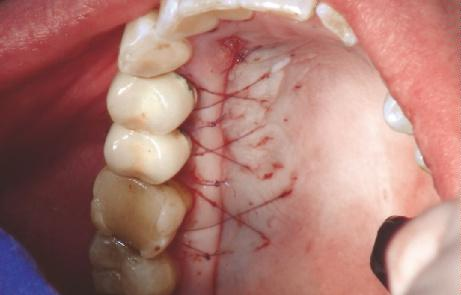
\includegraphics[width=221.4859pt,height=141.7323pt]{latexImage_97ec00442f9fe612164aa9da87bd6ec1.png}}
\put(293.9764,-601.1251){\fontsize{9}{1}\usefont{T1}{cmr}{m}{n}\selectfont\color{color_112230}Fig 3-7f  The connective tissue graft is placed inside the }
\put(293.9764,-612.1231){\fontsize{9}{1}\usefont{T1}{cmr}{m}{n}\selectfont\color{color_72488}prepared tunnel.}
\put(293.9764,-587.1336){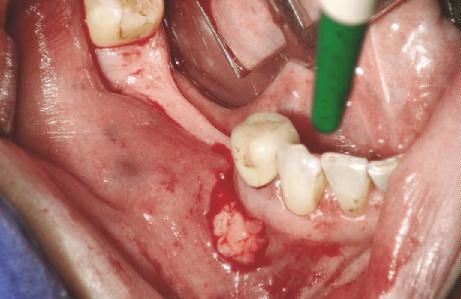
\includegraphics[width=221.1024pt,height=143.753pt]{latexImage_829058377c020b6934f59118a6d0b3c0.png}}
\put(58.7009,-222.8522){\fontsize{9}{1}\usefont{T1}{cmr}{m}{n}\selectfont\color{color_112230}Fig 3-7a  Thin soft tissue biotype in the atrophied right }
\put(58.7009,-233.8502){\fontsize{9}{1}\usefont{T1}{cmr}{m}{n}\selectfont\color{color_72488}mandible.}
\put(58.70083,-208.8365){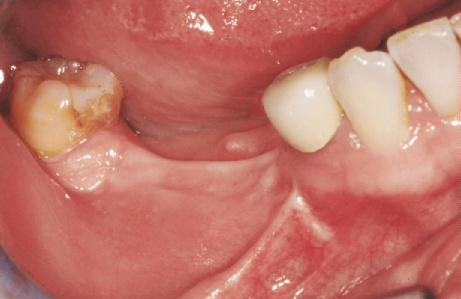
\includegraphics[width=221.1024pt,height=143.7045pt]{latexImage_8db9b4c97b3ccf5941cffbcc874e0c2d.png}}
\put(293.9764,-222.8522){\fontsize{9}{1}\usefont{T1}{cmr}{m}{n}\selectfont\color{color_112230}Fig}
\put(293.9764,-207.8503){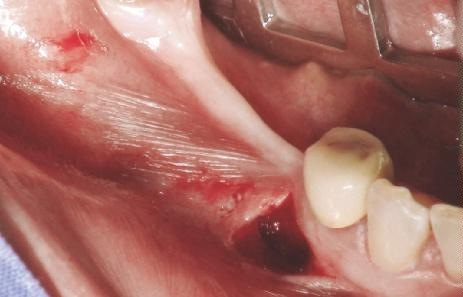
\includegraphics[width=222.043pt,height=142.7568pt]{latexImage_b15542cc86efdc321c03e34048278c92.png}}
\put(58.7009,-411.9887){\fontsize{9}{1}\usefont{T1}{cmr}{m}{n}\selectfont\color{color_112230}Fig 3-7c   Connective tissue graft harvested from the right }
\put(58.7009,-422.9867){\fontsize{9}{1}\usefont{T1}{cmr}{m}{n}\selectfont\color{color_72488}palate.}
\put(58.70083,-398.0667){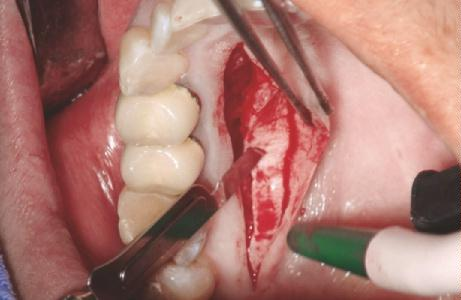
\includegraphics[width=221.1024pt,height=143.892pt]{latexImage_d9dc8de7d639189d2f042ad25a55c3be.png}}
\put(293.9764,-411.9887){\fontsize{9}{1}\usefont{T1}{cmr}{m}{n}\selectfont\color{color_112230}Fig 3-7d  Harvesting of a connective tissue graft from the }
\put(293.9764,-422.9867){\fontsize{9}{1}\usefont{T1}{cmr}{m}{n}\selectfont\color{color_72488}right palate.}
\put(292.8968,-396.9868){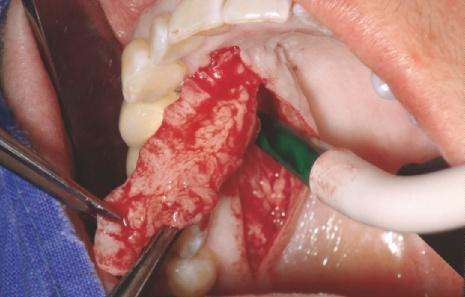
\includegraphics[width=223.2616pt,height=142.7798pt]{latexImage_26e638186b4f36166c01ecb6702eba5e.png}}
\end{picture}
\newpage
\begin{tikzpicture}[overlay]\path(0pt,0pt);\end{tikzpicture}
\begin{picture}(-5,0)(2.5,0)
\put(493.133,-754.1789){\fontsize{11}{1}\usefont{T1}{cmr}{m}{n}\selectfont\color{color_112230}93}
\put(255.698,-29.88385){\fontsize{11}{1}\usefont{T1}{cmr}{m}{n}\selectfont\color{color_112230}3.4}
\put(272.825,-29.88391){\fontsize{11}{1}\usefont{T1}{cmr}{m}{n}\selectfont\color{color_112230} Soft tissue management before augmentation}
\put(50.1969,-411.9887){\fontsize{9}{1}\usefont{T1}{cmr}{m}{n}\selectfont\color{color_112230}Fig 3-7i  Bone block grafting through the tunnel }
\put(50.1969,-422.9867){\fontsize{9}{1}\usefont{T1}{cmr}{m}{n}\selectfont\color{color_72488}approach.}
\put(50.1969,-398.0273){\includegraphics[width=221.1024pt,height=143.8134pt]{latexImage_48d406716498ef49037562854cb873fa.png}}
\put(285.4724,-411.9887){\fontsize{9}{1}\usefont{T1}{cmr}{m}{n}\selectfont\color{color_112230}Fig}
\put(284.4472,-396.9868){\includegraphics[width=223.153pt,height=141.7323pt]{latexImage_13492aeca99e171e950594e5ce8abdb0.png}}
\put(50.1969,-222.8522){\fontsize{9}{1}\usefont{T1}{cmr}{m}{n}\selectfont\color{color_112230}Fig}
\put(50.1969,-208.8607){\includegraphics[width=221.1024pt,height=143.753pt]{latexImage_ab7e4e280fc895c23b193e080d7e9ad3.png}}
\put(285.4724,-222.8522){\fontsize{9}{1}\usefont{T1}{cmr}{m}{n}\selectfont\color{color_112230}Fig}
\put(285.4725,-208.8556){\includegraphics[width=221.1024pt,height=143.7429pt]{latexImage_71913157f12060e0224825e542ad5187.png}}
\put(50.1969,-601.1251){\fontsize{9}{1}\usefont{T1}{cmr}{m}{n}\selectfont\color{color_112230}Fig}
\put(50.1969,-587.1448){\includegraphics[width=221.1023pt,height=143.7753pt]{latexImage_4af8ab5d7ca8cd173fef88bbf10d4cc2.png}}
\put(285.4724,-601.1251){\fontsize{9}{1}\usefont{T1}{cmr}{m}{n}\selectfont\color{color_112230}Fig}
\put(284.4369,-586.1233){\includegraphics[width=223.1736pt,height=141.7323pt]{latexImage_ce5f4d65cbd7fda1cb99a69078e49099.png}}
\put(50.1969,-645.7559){\fontsize{10.8}{1}\usefont{T1}{cmr}{m}{n}\selectfont\color{color_72488}many described harvesting techniques used to }
\put(50.1969,-660.7571){\fontsize{10.8}{1}\usefont{T1}{cmr}{m}{n}\selectfont\color{color_72488}dissect subepithelial grafts,}
\put(179.5063,-658.0559){\fontsize{6.48}{1}\usefont{T1}{cmr}{m}{n}\selectfont\color{color_72488}83,107}
\put(201.0843,-660.7559){\fontsize{10.8}{1}\usefont{T1}{cmr}{m}{n}\selectfont\color{color_72488} as it has been }
\put(50.1975,-675.7571){\fontsize{10.8}{1}\usefont{T1}{cmr}{m}{n}\selectfont\color{color_72488}found to improve postoperative healing and pa}
\put(267.703,-675.756){\fontsize{10.8}{1}\usefont{T1}{cmr}{m}{n}\selectfont\color{color_72488}-}
\put(50.19749,-690.7562){\fontsize{10.8}{1}\usefont{T1}{cmr}{m}{n}\selectfont\color{color_72488}tient morbidity. The technique involves a hori-}
\put(50.19749,-705.7563){\fontsize{10.8}{1}\usefont{T1}{cmr}{m}{n}\selectfont\color{color_72488}zontal incision on the palatal side, followed by }
\put(50.19749,-720.7574){\fontsize{10.8}{1}\usefont{T1}{cmr}{m}{n}\selectfont\color{color_72488}a sharp undermining dissection. The wound }
\put(285.4755,-645.7623){\fontsize{10.8}{1}\usefont{T1}{cmr}{m}{n}\selectfont\color{color_72488}margins can be optimally stabilized during later }
\put(285.4755,-660.7635){\fontsize{10.8}{1}\usefont{T1}{cmr}{m}{n}\selectfont\color{color_72488}suturing if the harvesting incision is 1 to 1.5}
\put(486.0093,-660.7631){\fontsize{10.8}{1}\usefont{T1}{cmr}{m}{n}\selectfont\color{color_72488} mm }
\put(285.4749,-675.7643){\fontsize{10.8}{1}\usefont{T1}{cmr}{m}{n}\selectfont\color{color_72488}from the first incision. Depending on the pa}
\put(502.9782,-675.7557){\fontsize{10.8}{1}\usefont{T1}{cmr}{m}{n}\selectfont\color{color_72488}-}
\put(285.4727,-690.7558){\fontsize{10.8}{1}\usefont{T1}{cmr}{m}{n}\selectfont\color{color_72488}tient, a decision needs to be made as to wheth-}
\put(285.4727,-705.7559){\fontsize{10.8}{1}\usefont{T1}{cmr}{m}{n}\selectfont\color{color_72488}er the graft should be elevated from the bone }
\put(285.4727,-720.7571){\fontsize{10.8}{1}\usefont{T1}{cmr}{m}{n}\selectfont\color{color_72488}bluntly or by using a further split-flap  dissection. }
\end{picture}
\newpage
\begin{tikzpicture}[overlay]\path(0pt,0pt);\end{tikzpicture}
\begin{picture}(-5,0)(2.5,0)
\put(58.7009,-754.1789){\fontsize{11}{1}\usefont{T1}{cmr}{m}{n}\selectfont\color{color_112230}94}
\put(58.7009,-29.88385){\fontsize{11}{1}\usefont{T1}{cmr}{m}{n}\selectfont\color{color_112230}3}
\put(64.9269,-29.88391){\fontsize{11}{1}\usefont{T1}{cmr}{m}{n}\selectfont\color{color_112230} Soft tissue management and bone augmentation in implantology}
\put(58.7008,-480.7559){\fontsize{10.8}{1}\usefont{T1}{cmr}{m}{n}\selectfont\color{color_72488}The blunt approach enables the excision of a }
\put(58.7008,-495.7571){\fontsize{10.8}{1}\usefont{T1}{cmr}{m}{n}\selectfont\color{color_72488}more voluminous and more stable graft, incor}
\put(276.2074,-495.756){\fontsize{10.8}{1}\usefont{T1}{cmr}{m}{n}\selectfont\color{color_72488}-}
\put(58.7008,-510.7562){\fontsize{10.8}{1}\usefont{T1}{cmr}{m}{n}\selectfont\color{color_72488}porating the periosteum but at the price of }
\put(58.7008,-525.7573){\fontsize{10.8}{1}\usefont{T1}{cmr}{m}{n}\selectfont\color{color_72488}slightly greater patient morbidity. For suture }
\put(58.7008,-540.7585){\fontsize{10.8}{1}\usefont{T1}{cmr}{m}{n}\selectfont\color{color_72488}care, a combination of continuous sling sutures, }
\put(58.7008,-555.7598){\fontsize{10.8}{1}\usefont{T1}{cmr}{m}{n}\selectfont\color{color_72488}simple interrupted sutures, and a palate plate is }
\put(58.7008,-570.7609){\fontsize{10.8}{1}\usefont{T1}{cmr}{m}{n}\selectfont\color{color_72488}recommended (Fig}
\put(146.0674,-570.7607){\fontsize{10.8}{1}\usefont{T1}{cmr}{m}{n}\selectfont\color{color_72488} 3-7e).}
\put(72.8704,-585.7619){\fontsize{10.8}{1}\usefont{T1}{cmr}{m}{n}\selectfont\color{color_72488}If connective tissue with a higher ratio of col}
\put(276.2074,-585.7554){\fontsize{10.8}{1}\usefont{T1}{cmr}{m}{n}\selectfont\color{color_72488}-}
\put(58.7008,-600.7556){\fontsize{10.8}{1}\usefont{T1}{cmr}{m}{n}\selectfont\color{color_72488}lagen and less fatty and glandular tissue is re-}
\put(58.7008,-615.7557){\fontsize{10.8}{1}\usefont{T1}{cmr}{m}{n}\selectfont\color{color_72488}quired, a deepithelialized gingival/connective }
\put(58.7008,-630.7569){\fontsize{10.8}{1}\usefont{T1}{cmr}{m}{n}\selectfont\color{color_72488}tissue graft is recommended. Alternatively, the }
\put(58.7008,-645.7581){\fontsize{10.8}{1}\usefont{T1}{cmr}{m}{n}\selectfont\color{color_72488}tuberosity region is recommended as a second}
\put(276.2074,-645.7559){\fontsize{10.8}{1}\usefont{T1}{cmr}{m}{n}\selectfont\color{color_72488}-}
\put(58.7008,-660.756){\fontsize{10.8}{1}\usefont{T1}{cmr}{m}{n}\selectfont\color{color_72488}ary donor site. Grafts gained using a distal wedge }
\put(58.7008,-675.7573){\fontsize{10.8}{1}\usefont{T1}{cmr}{m}{n}\selectfont\color{color_72488}excision will shrink less due to their structure, }
\put(58.7008,-690.7584){\fontsize{10.8}{1}\usefont{T1}{cmr}{m}{n}\selectfont\color{color_72488}and have a special form, which makes revascu}
\put(276.2074,-690.7563){\fontsize{10.8}{1}\usefont{T1}{cmr}{m}{n}\selectfont\color{color_72488}-}
\put(58.7008,-705.7564){\fontsize{10.8}{1}\usefont{T1}{cmr}{m}{n}\selectfont\color{color_72488}larization difficult. For this reason, the tuberosi-}
\put(58.7008,-720.7565){\fontsize{10.8}{1}\usefont{T1}{cmr}{m}{n}\selectfont\color{color_72488}ty region remains the secondary donor site.}
\put(308.1484,-270.7529){\fontsize{10.8}{1}\usefont{T1}{cmr}{m}{n}\selectfont\color{color_72488}In addition to own tissue-specific proteins, }
\put(293.9788,-285.7542){\fontsize{10.8}{1}\usefont{T1}{cmr}{m}{n}\selectfont\color{color_72488}autologous connective tissue grafts also con}
\put(511.4822,-285.7563){\fontsize{10.8}{1}\usefont{T1}{cmr}{m}{n}\selectfont\color{color_72488}-}
\put(293.9767,-300.7564){\fontsize{10.8}{1}\usefont{T1}{cmr}{m}{n}\selectfont\color{color_72488}tain a significant number of fibroblasts, the }
\put(293.9767,-315.7576){\fontsize{10.8}{1}\usefont{T1}{cmr}{m}{n}\selectfont\color{color_72488}majority of which are accessible for initial plas}
\put(511.4822,-315.7565){\fontsize{10.8}{1}\usefont{T1}{cmr}{m}{n}\selectfont\color{color_72488}-}
\put(293.9767,-330.7567){\fontsize{10.8}{1}\usefont{T1}{cmr}{m}{n}\selectfont\color{color_72488}matic circulation and the revascularization that }
\put(293.9767,-345.7578){\fontsize{10.8}{1}\usefont{T1}{cmr}{m}{n}\selectfont\color{color_72488}follows, for which reason they have a more fa}
\put(511.4822,-345.7568){\fontsize{10.8}{1}\usefont{T1}{cmr}{m}{n}\selectfont\color{color_72488}-}
\put(293.9767,-360.7569){\fontsize{10.8}{1}\usefont{T1}{cmr}{m}{n}\selectfont\color{color_72488}vorable prognosis. }
\put(293.9764,-402.933){\fontsize{12.5}{1}\usefont{T1}{cmr}{m}{n}\selectfont\color{color_112230}3.4.4 Punch technique}
\put(293.9764,-420.7559){\fontsize{10.8}{1}\usefont{T1}{cmr}{m}{n}\selectfont\color{color_72488}If there are no acute inflammatory symptoms, }
\put(293.9764,-435.7571){\fontsize{10.8}{1}\usefont{T1}{cmr}{m}{n}\selectfont\color{color_72488}the so-called ‘punch technique’}
\put(443.1797,-433.0558){\fontsize{6.48}{1}\usefont{T1}{cmr}{m}{n}\selectfont\color{color_72488}90}
\put(450.9685,-435.7559){\fontsize{10.8}{1}\usefont{T1}{cmr}{m}{n}\selectfont\color{color_72488} – involving a }
\put(293.9797,-450.7571){\fontsize{10.8}{1}\usefont{T1}{cmr}{m}{n}\selectfont\color{color_72488}combined graft consisting of connective tissue }
\put(293.9797,-465.7583){\fontsize{10.8}{1}\usefont{T1}{cmr}{m}{n}\selectfont\color{color_72488}and epithelial parts – can also be used for the }
\put(293.9797,-480.7595){\fontsize{10.8}{1}\usefont{T1}{cmr}{m}{n}\selectfont\color{color_72488}closure of extraction or explantation alveoli. This }
\put(293.9797,-495.7607){\fontsize{10.8}{1}\usefont{T1}{cmr}{m}{n}\selectfont\color{color_72488}technique results in an optimal stability of the }
\put(293.9797,-510.7618){\fontsize{10.8}{1}\usefont{T1}{cmr}{m}{n}\selectfont\color{color_72488}coagulum in the alveolus, and it compensates }
\put(293.9797,-525.7631){\fontsize{10.8}{1}\usefont{T1}{cmr}{m}{n}\selectfont\color{color_72488}for the volume and keratinization of the soft tis}
\put(511.482,-525.7555){\fontsize{10.8}{1}\usefont{T1}{cmr}{m}{n}\selectfont\color{color_72488}-}
\put(293.9754,-540.7556){\fontsize{10.8}{1}\usefont{T1}{cmr}{m}{n}\selectfont\color{color_72488}sue. The graft can be harvested from the tubera }
\put(293.9754,-555.7568){\fontsize{10.8}{1}\usefont{T1}{cmr}{m}{n}\selectfont\color{color_72488}behind the last molar in cases where there is a }
\put(293.9754,-570.758){\fontsize{10.8}{1}\usefont{T1}{cmr}{m}{n}\selectfont\color{color_72488}wide keratinized gingiva in this area (Fig}
\put(478.786,-570.7583){\fontsize{10.8}{1}\usefont{T1}{cmr}{m}{n}\selectfont\color{color_72488} 3-8a to }
\put(293.9764,-585.7595){\fontsize{10.8}{1}\usefont{T1}{cmr}{m}{n}\selectfont\color{color_72488}j) or from the palate in the premolar area. In the }
\put(293.9764,-600.7607){\fontsize{10.8}{1}\usefont{T1}{cmr}{m}{n}\selectfont\color{color_72488}case of the palate, a rotated punch bur can be }
\put(293.9764,-615.7619){\fontsize{10.8}{1}\usefont{T1}{cmr}{m}{n}\selectfont\color{color_72488}used to facilitate the harvesting procedure }
\put(293.9764,-630.7631){\fontsize{10.8}{1}\usefont{T1}{cmr}{m}{n}\selectfont\color{color_72488}(Fig 3-9a to l). In the case of the graft being }
\put(293.9764,-645.7643){\fontsize{10.8}{1}\usefont{T1}{cmr}{m}{n}\selectfont\color{color_72488}harvested from the tubera, an incision is made }
\put(293.9764,-660.7655){\fontsize{10.8}{1}\usefont{T1}{cmr}{m}{n}\selectfont\color{color_72488}in the middle of the connective tissue area that }
\put(293.9764,-675.7667){\fontsize{10.8}{1}\usefont{T1}{cmr}{m}{n}\selectfont\color{color_72488}will create two strips of connective tissue by }
\put(293.9764,-690.7679){\fontsize{10.8}{1}\usefont{T1}{cmr}{m}{n}\selectfont\color{color_72488}keeping a central epithelial area, with a diame}
\put(511.483,-690.756){\fontsize{10.8}{1}\usefont{T1}{cmr}{m}{n}\selectfont\color{color_72488}-}
\put(293.9764,-705.7562){\fontsize{10.8}{1}\usefont{T1}{cmr}{m}{n}\selectfont\color{color_72488}ter corresponding to that of the extraction sock-}
\put(293.9764,-720.7563){\fontsize{10.8}{1}\usefont{T1}{cmr}{m}{n}\selectfont\color{color_72488}et. Split-thickness flaps are dissected without }
\put(58.7009,-222.8522){\fontsize{9}{1}\usefont{T1}{cmr}{m}{n}\selectfont\color{color_112230}Fig 3-8a  Clinical situation before extraction of the left }
\put(58.7009,-233.8502){\fontsize{9}{1}\usefont{T1}{cmr}{m}{n}\selectfont\color{color_72488}central incisor due to a length fracture.}
\put(58.70083,-207.8503){\includegraphics[width=221.1023pt,height=142.7764pt]{latexImage_d3069e7c2c32cc7eece0b90de170c32b.png}}
\put(293.9764,-222.8522){\fontsize{9}{1}\usefont{T1}{cmr}{m}{n}\selectfont\color{color_112230}Fig}
\put(292.9169,-207.8503){\includegraphics[width=223.2214pt,height=142.7772pt]{latexImage_787536133bf783eeddd193ce9099d927.png}}
\put(58.7008,-418.1593){\fontsize{9}{1}\usefont{T1}{cmr}{m}{n}\selectfont\color{color_112230}Fig 3-8c  Clinical situation after atraumatic extraction of }
\put(58.70081,-429.1573){\fontsize{9}{1}\usefont{T1}{cmr}{m}{n}\selectfont\color{color_72488}the central incisor}
\put(58.70083,-404.1774){\includegraphics[width=221.1023pt,height=143.7724pt]{latexImage_d9c3f48780e42334836c43b2a2d98c89.png}}
\end{picture}
\newpage
\begin{tikzpicture}[overlay]\path(0pt,0pt);\end{tikzpicture}
\begin{picture}(-5,0)(2.5,0)
\put(493.133,-754.1789){\fontsize{11}{1}\usefont{T1}{cmr}{m}{n}\selectfont\color{color_112230}95}
\put(255.698,-29.88385){\fontsize{11}{1}\usefont{T1}{cmr}{m}{n}\selectfont\color{color_112230}3.4}
\put(272.825,-29.88391){\fontsize{11}{1}\usefont{T1}{cmr}{m}{n}\selectfont\color{color_112230} Soft tissue management before augmentation}
\put(208.4651,-279.5451){\fontsize{9}{1}\usefont{T1}{cmr}{m}{n}\selectfont\color{color_112230}Fig}
\put(207.3987,-265.5555){\includegraphics[width=144.768pt,height=200.448pt]{latexImage_8cddb4c23d2ec47c71f3926abf474293.png}}
\put(363.8986,-279.5451){\fontsize{9}{1}\usefont{T1}{cmr}{m}{n}\selectfont\color{color_112230}Fig}
\put(363.8986,-265.5837){\includegraphics[width=142.6762pt,height=200.0529pt]{latexImage_3367e1a7b32deedb18706c78d6270124.png}}
\put(50.1969,-279.5451){\fontsize{9}{1}\usefont{T1}{cmr}{m}{n}\selectfont\color{color_112230}Fig 3-8d  Harvesting of an epithelial/}
\put(50.1969,-290.5431){\fontsize{9}{1}\usefont{T1}{cmr}{m}{n}\selectfont\color{color_72488}connective tissue graft from the tuber }
\put(50.1969,-301.5411){\fontsize{9}{1}\usefont{T1}{cmr}{m}{n}\selectfont\color{color_72488}area.}
\put(50.19689,-265.5824){\includegraphics[width=142.6762pt,height=200.5033pt]{latexImage_a60c467c09bd08372c13abd91848fc5d.png}}
\put(50.1969,-494.4497){\fontsize{9}{1}\usefont{T1}{cmr}{m}{n}\selectfont\color{color_112230}Fig 3-8g  The connective tissue part is cut in the middle, }
\put(50.1969,-505.4477){\fontsize{9}{1}\usefont{T1}{cmr}{m}{n}\selectfont\color{color_72488}obtaining two wings of connective tissue.}
\put(49.16214,-480.4786){\includegraphics[width=223.1376pt,height=143.7936pt]{latexImage_b7e729f7b1302eb4ff6731037e571d05.png}}
\put(285.4724,-494.4497){\fontsize{9}{1}\usefont{T1}{cmr}{m}{n}\selectfont\color{color_112230}Fig 3-8h  The two connective tissue wings are stabilized }
\put(285.4724,-505.4477){\fontsize{9}{1}\usefont{T1}{cmr}{m}{n}\selectfont\color{color_72488}with sutures under the buccal and palatal flap, closing the }
\put(285.4724,-516.4457){\fontsize{9}{1}\usefont{T1}{cmr}{m}{n}\selectfont\color{color_72488}socket with the epithelial part.}
\put(285.4725,-480.468){\includegraphics[width=221.1023pt,height=143.7724pt]{latexImage_f5f696f88d764e0b91fa9589dc6dbd36.png}}
\put(50.1969,-709.3543){\fontsize{9}{1}\usefont{T1}{cmr}{m}{n}\selectfont\color{color_112230}Fig 3-8i  Clinical appearance 6 weeks postoperatively: }
\put(50.1969,-720.3523){\fontsize{9}{1}\usefont{T1}{cmr}{m}{n}\selectfont\color{color_72488}vestibular view}
\put(47.62022,-699.2441){\includegraphics[width=226.2557pt,height=151.5156pt]{latexImage_d4ee24f9d055af781ece9c50905fe0a4.png}}
\put(285.4724,-709.3543){\fontsize{9}{1}\usefont{T1}{cmr}{m}{n}\selectfont\color{color_112230}Fig 3-8j  Occlusal view 10 weeks postoperatively docu-}
\put(285.4724,-720.3523){\fontsize{9}{1}\usefont{T1}{cmr}{m}{n}\selectfont\color{color_72488}menting the soft tissue stability}
\put(284.413,-694.3525){\includegraphics[width=223.2214pt,height=142.7772pt]{latexImage_1c82476f1f339a26010253f22059bc2c.png}}
\end{picture}
\newpage
\begin{tikzpicture}[overlay]\path(0pt,0pt);\end{tikzpicture}
\begin{picture}(-5,0)(2.5,0)
\put(58.7009,-754.1789){\fontsize{11}{1}\usefont{T1}{cmr}{m}{n}\selectfont\color{color_112230}96}
\put(58.7009,-29.88385){\fontsize{11}{1}\usefont{T1}{cmr}{m}{n}\selectfont\color{color_112230}3}
\put(64.9269,-29.88391){\fontsize{11}{1}\usefont{T1}{cmr}{m}{n}\selectfont\color{color_112230} Soft tissue management and bone augmentation in implantology}
\put(58.7009,-687.3543){\fontsize{9}{1}\usefont{T1}{cmr}{m}{n}\selectfont\color{color_112230}Fig 3-9e  Soft tissue graft sealing the socket and stabi-}
\put(58.70089,-698.3523){\fontsize{9}{1}\usefont{T1}{cmr}{m}{n}\selectfont\color{color_72488}lized with 6-0 sutures.}
\put(58.70083,-673.4166){\includegraphics[width=221.1024pt,height=143.8604pt]{latexImage_f9e2de54b72dd2d2eb19d3f119a82fd0.png}}
\put(293.9764,-687.3543){\fontsize{9}{1}\usefont{T1}{cmr}{m}{n}\selectfont\color{color_112230}Fig}
\put(293.8267,-672.3524){\includegraphics[width=221.4017pt,height=142.7588pt]{latexImage_53dfd5a7bcb46655649a4949904e3b9a.png}}
\put(58.7009,-222.8522){\fontsize{9}{1}\usefont{T1}{cmr}{m}{n}\selectfont\color{color_112230}Fig 3-9a  Right central incisor has to be removed due to }
\put(58.7009,-233.8502){\fontsize{9}{1}\usefont{T1}{cmr}{m}{n}\selectfont\color{color_72488}a severe resorption. The left central and lateral incisors }
\put(58.7009,-244.8482){\fontsize{9}{1}\usefont{T1}{cmr}{m}{n}\selectfont\color{color_72488}are already replaced by implants.}
\put(57.81196,-207.8503){\includegraphics[width=222.8801pt,height=141.7323pt]{latexImage_5f2ff43abe4d2da25f3b7d2b70f38733.png}}
\put(293.9764,-222.8522){\fontsize{9}{1}\usefont{T1}{cmr}{m}{n}\selectfont\color{color_112230}Fig}
\put(292.8712,-207.8503){\includegraphics[width=223.236pt,height=142.776pt]{latexImage_92ad53b62800b71b8f778e7d6dc4c1af.png}}
\put(58.7009,-455.1033){\fontsize{9}{1}\usefont{T1}{cmr}{m}{n}\selectfont\color{color_112230}Fig 3-9c  Harvesting an epithelial/connective tissue graft }
\put(58.7009,-466.1013){\fontsize{9}{1}\usefont{T1}{cmr}{m}{n}\selectfont\color{color_72488}from the lateral palate using a soft tissue punch.}
\put(58.70083,-441.1086){\includegraphics[width=221.1024pt,height=143.7463pt]{latexImage_6acb341240d36c975aea01382b42c34f.png}}
\put(293.9764,-455.1033){\fontsize{9}{1}\usefont{T1}{cmr}{m}{n}\selectfont\color{color_112230}Fig}
\put(292.9514,-441.1888){\includegraphics[width=223.1328pt,height=143.8272pt]{latexImage_1a2e7a323beb808295cb734c5986a058.png}}
\end{picture}
\newpage
\begin{tikzpicture}[overlay]\path(0pt,0pt);\end{tikzpicture}
\begin{picture}(-5,0)(2.5,0)
\put(493.133,-754.1789){\fontsize{11}{1}\usefont{T1}{cmr}{m}{n}\selectfont\color{color_112230}97}
\put(255.698,-29.88385){\fontsize{11}{1}\usefont{T1}{cmr}{m}{n}\selectfont\color{color_112230}3.4}
\put(272.825,-29.88391){\fontsize{11}{1}\usefont{T1}{cmr}{m}{n}\selectfont\color{color_112230} Soft tissue management before augmentation}
\put(50.1969,-222.8522){\fontsize{9}{1}\usefont{T1}{cmr}{m}{n}\selectfont\color{color_112230}Fig}
\put(50.1969,-208.8818){\includegraphics[width=221.1023pt,height=143.7952pt]{latexImage_1f280159ce1ef74d550e0bdbe7ac8516.png}}
\put(285.4724,-222.8522){\fontsize{9}{1}\usefont{T1}{cmr}{m}{n}\selectfont\color{color_112230}Fig 3-9h  Clinical situation 2 months after the soft tissue }
\put(285.4724,-233.8502){\fontsize{9}{1}\usefont{T1}{cmr}{m}{n}\selectfont\color{color_72488}grafting documenting the good soft tissue quantity and }
\put(285.4724,-244.8482){\fontsize{9}{1}\usefont{T1}{cmr}{m}{n}\selectfont\color{color_72488}quality prior to the bone grafting procedure.}
\put(285.4725,-208.0012){\includegraphics[width=221.1024pt,height=142.034pt]{latexImage_176b5bb32c84c606e93b3ca01b790029.png}}
\put(50.1969,-687.3543){\fontsize{9}{1}\usefont{T1}{cmr}{m}{n}\selectfont\color{color_112230}Fig 3-9k  Good soft tissue healing 2 weeks postoperative-}
\put(50.19691,-698.3523){\fontsize{9}{1}\usefont{T1}{cmr}{m}{n}\selectfont\color{color_72488}ly. The soft tissue improvement prior to bone augmenta-}
\put(50.19691,-709.3503){\fontsize{9}{1}\usefont{T1}{cmr}{m}{n}\selectfont\color{color_72488}tion reduced the risk of tissue necrosis, with exposure of }
\put(50.19691,-720.3483){\fontsize{9}{1}\usefont{T1}{cmr}{m}{n}\selectfont\color{color_72488}the grafted bone.}
\put(50.19689,-672.3525){\includegraphics[width=221.1024pt,height=142.7888pt]{latexImage_b13efb86342236c7ef147de0180bda04.png}}
\put(50.1969,-455.1033){\fontsize{9}{1}\usefont{T1}{cmr}{m}{n}\selectfont\color{color_112230}Fig 3-9i  Implant insertion inside the bony contours. Note }
\put(50.1969,-466.1013){\fontsize{9}{1}\usefont{T1}{cmr}{m}{n}\selectfont\color{color_72488}the bony defect on the vestibular side.}
\put(50.1969,-441.1501){\includegraphics[width=221.1024pt,height=143.8293pt]{latexImage_5b893b94b336ac22cc0d33925fdbaf06.png}}
\put(285.4724,-455.1033){\fontsize{9}{1}\usefont{T1}{cmr}{m}{n}\selectfont\color{color_112230}Fig 3-9j  The defect on the vestibular side is rebuilt with }
\put(285.4724,-466.1013){\fontsize{9}{1}\usefont{T1}{cmr}{m}{n}\selectfont\color{color_72488}a mandibular bone block graft.}
\put(284.438,-440.1016){\includegraphics[width=223.1712pt,height=142.7784pt]{latexImage_232b1b0954f07961a828aafe1cf39377.png}}
\put(285.4724,-687.3543){\fontsize{9}{1}\usefont{T1}{cmr}{m}{n}\selectfont\color{color_112230}Fig 3-9l  Clinical aspect after implant exposure present-}
\put(285.4724,-698.3523){\fontsize{9}{1}\usefont{T1}{cmr}{m}{n}\selectfont\color{color_72488}ing good hard and soft tissue support.}
\put(285.4725,-672.3525){\includegraphics[width=222.1297pt,height=142.769pt]{latexImage_471a37b2546c45a4aaeba89a85a468f7.png}}
\end{picture}
\newpage
\begin{tikzpicture}[overlay]\path(0pt,0pt);\end{tikzpicture}
\begin{picture}(-5,0)(2.5,0)
\put(58.7009,-754.1789){\fontsize{11}{1}\usefont{T1}{cmr}{m}{n}\selectfont\color{color_112230}98}
\put(58.7009,-29.88385){\fontsize{11}{1}\usefont{T1}{cmr}{m}{n}\selectfont\color{color_112230}3}
\put(64.9269,-29.88391){\fontsize{11}{1}\usefont{T1}{cmr}{m}{n}\selectfont\color{color_112230} Soft tissue management and bone augmentation in implantology}
\put(58.7008,-75.75592){\fontsize{10.8}{1}\usefont{T1}{cmr}{m}{n}\selectfont\color{color_72488}incisions in the area of the alveolus on both the }
\put(58.7008,-90.75714){\fontsize{10.8}{1}\usefont{T1}{cmr}{m}{n}\selectfont\color{color_72488}buccal and oral sides using the tunnel tech}
\put(276.2074,-90.75604){\fontsize{10.8}{1}\usefont{T1}{cmr}{m}{n}\selectfont\color{color_72488}-}
\put(58.7008,-105.7562){\fontsize{10.8}{1}\usefont{T1}{cmr}{m}{n}\selectfont\color{color_72488}nique. The size should be double that of the }
\put(58.7008,-120.7574){\fontsize{10.8}{1}\usefont{T1}{cmr}{m}{n}\selectfont\color{color_72488}connective tissue strips, which can be fixed buc}
\put(276.2074,-120.7563){\fontsize{10.8}{1}\usefont{T1}{cmr}{m}{n}\selectfont\color{color_72488}-}
\put(58.7008,-135.7564){\fontsize{10.8}{1}\usefont{T1}{cmr}{m}{n}\selectfont\color{color_72488}cally and orally with two sling sutures. For final }
\put(58.7008,-150.7576){\fontsize{10.8}{1}\usefont{T1}{cmr}{m}{n}\selectfont\color{color_72488}wound care, the epithelial area of the graft is }
\put(58.7008,-165.7589){\fontsize{10.8}{1}\usefont{T1}{cmr}{m}{n}\selectfont\color{color_72488}adapted to the surrounding epithelium. As a re}
\put(276.2074,-165.7567){\fontsize{10.8}{1}\usefont{T1}{cmr}{m}{n}\selectfont\color{color_72488}-}
\put(58.7008,-180.7568){\fontsize{10.8}{1}\usefont{T1}{cmr}{m}{n}\selectfont\color{color_72488}sult, the areas covered with epithelium are not }
\put(58.7008,-195.7581){\fontsize{10.8}{1}\usefont{T1}{cmr}{m}{n}\selectfont\color{color_72488}covered with an auxiliary flap and are therefore }
\put(58.7008,-210.7593){\fontsize{10.8}{1}\usefont{T1}{cmr}{m}{n}\selectfont\color{color_72488}exposed in the oral cavity. The lobes gained, }
\put(58.7008,-225.7605){\fontsize{10.8}{1}\usefont{T1}{cmr}{m}{n}\selectfont\color{color_72488}however, ensure the improved revascularization }
\put(58.7008,-240.7617){\fontsize{10.8}{1}\usefont{T1}{cmr}{m}{n}\selectfont\color{color_72488}and diffusion of the graft and the additional in}
\put(276.2074,-240.7574){\fontsize{10.8}{1}\usefont{T1}{cmr}{m}{n}\selectfont\color{color_72488}-}
\put(58.7008,-255.7575){\fontsize{10.8}{1}\usefont{T1}{cmr}{m}{n}\selectfont\color{color_72488}crease in volume in the bucco-crestal region.}
\put(267.3892,-255.7559){\fontsize{10.8}{1}\usefont{T1}{cmr}{m}{n}\selectfont\color{color_252189} }
\put(58.7008,-292.933){\fontsize{12.5}{1}\usefont{T1}{cmr}{m}{n}\selectfont\color{color_112230}3.4.5 Palatal pedicle connective tissue }
\put(98.3883,-307.433){\fontsize{12.5}{1}\usefont{T1}{cmr}{m}{n}\selectfont\color{color_112230}flaps}
\put(58.7008,-330.7559){\fontsize{10.8}{1}\usefont{T1}{cmr}{m}{n}\selectfont\color{color_72488}Damage to bone but also to soft tissue can be so }
\put(58.7008,-345.7571){\fontsize{10.8}{1}\usefont{T1}{cmr}{m}{n}\selectfont\color{color_72488}severe after the extraction of a tooth or the ex}
\put(276.2074,-345.756){\fontsize{10.8}{1}\usefont{T1}{cmr}{m}{n}\selectfont\color{color_72488}-}
\put(58.7008,-360.7562){\fontsize{10.8}{1}\usefont{T1}{cmr}{m}{n}\selectfont\color{color_72488}plantation of an implant, particularly in the case }
\put(58.7008,-375.7574){\fontsize{10.8}{1}\usefont{T1}{cmr}{m}{n}\selectfont\color{color_72488}of failed augmentation procedures, that closure }
\put(58.7008,-390.7585){\fontsize{10.8}{1}\usefont{T1}{cmr}{m}{n}\selectfont\color{color_72488}using the punch technique is no longer ade}
\put(276.2074,-390.7564){\fontsize{10.8}{1}\usefont{T1}{cmr}{m}{n}\selectfont\color{color_72488}-}
\put(58.7008,-405.7565){\fontsize{10.8}{1}\usefont{T1}{cmr}{m}{n}\selectfont\color{color_72488}quate to ensure the required volume. In such }
\put(58.7008,-420.7577){\fontsize{10.8}{1}\usefont{T1}{cmr}{m}{n}\selectfont\color{color_72488}cases, coverage of the extraction socket can also }
\put(58.7008,-435.7589){\fontsize{10.8}{1}\usefont{T1}{cmr}{m}{n}\selectfont\color{color_72488}be safely achieved after immediate }
\put(221.5756,-435.7583){\fontsize{10.8}{1}\usefont{T1}{cmr}{m}{n}\selectfont\color{color_72488} implantation }
\put(58.7008,-450.7595){\fontsize{10.8}{1}\usefont{T1}{cmr}{m}{n}\selectfont\color{color_72488}with a palatal pedicle connective  tissue flap. }
\put(58.7008,-465.7607){\fontsize{10.8}{1}\usefont{T1}{cmr}{m}{n}\selectfont\color{color_72488}The existing soft tissue deficit can be evened }
\put(58.7008,-480.7619){\fontsize{10.8}{1}\usefont{T1}{cmr}{m}{n}\selectfont\color{color_72488}out and covered by creating a mucoperiosteal }
\put(58.7008,-495.7631){\fontsize{10.8}{1}\usefont{T1}{cmr}{m}{n}\selectfont\color{color_72488}flap using the Rehrmann technique}
\put(228.5131,-493.0559){\fontsize{6.48}{1}\usefont{T1}{cmr}{m}{n}\selectfont\color{color_72488}163}
\put(240.1964,-495.7559){\fontsize{10.8}{1}\usefont{T1}{cmr}{m}{n}\selectfont\color{color_72488} or by a }
\put(58.70238,-510.7571){\fontsize{10.8}{1}\usefont{T1}{cmr}{m}{n}\selectfont\color{color_72488}connective tissue graft.}
\put(164.7292,-508.0559){\fontsize{6.48}{1}\usefont{T1}{cmr}{m}{n}\selectfont\color{color_72488}35}
\put(172.518,-510.7559){\fontsize{10.8}{1}\usefont{T1}{cmr}{m}{n}\selectfont\color{color_72488} The use of palatal ped-}
\put(58.70004,-525.756){\fontsize{10.8}{1}\usefont{T1}{cmr}{m}{n}\selectfont\color{color_72488}icle connective tissue flaps is of course limited }
\put(58.70004,-540.7572){\fontsize{10.8}{1}\usefont{T1}{cmr}{m}{n}\selectfont\color{color_72488}to the maxilla for anatomical reasons. A pedicle }
\put(58.70004,-555.7584){\fontsize{10.8}{1}\usefont{T1}{cmr}{m}{n}\selectfont\color{color_72488}graft from the palate, which at least retains a }
\put(58.70004,-570.7596){\fontsize{10.8}{1}\usefont{T1}{cmr}{m}{n}\selectfont\color{color_72488}minimal vascular supply, has a better prognosis }
\put(58.70004,-585.7609){\fontsize{10.8}{1}\usefont{T1}{cmr}{m}{n}\selectfont\color{color_72488}in areas previously operated on multiple times }
\put(58.70004,-600.762){\fontsize{10.8}{1}\usefont{T1}{cmr}{m}{n}\selectfont\color{color_72488}with an accordingly degraded recipient bed, and }
\put(58.70004,-615.7632){\fontsize{10.8}{1}\usefont{T1}{cmr}{m}{n}\selectfont\color{color_72488}leads to safer coverage than free grafts without }
\put(58.70004,-630.7645){\fontsize{10.8}{1}\usefont{T1}{cmr}{m}{n}\selectfont\color{color_72488}any arterial vascular connections. Grafts of a }
\put(58.70004,-645.7656){\fontsize{10.8}{1}\usefont{T1}{cmr}{m}{n}\selectfont\color{color_72488}thickness of 2 to 5}
\put(151.2892,-645.7655){\fontsize{10.8}{1}\usefont{T1}{cmr}{m}{n}\selectfont\color{color_72488} mm or thicker}
\put(221.415,-643.0559){\fontsize{6.48}{1}\usefont{T1}{cmr}{m}{n}\selectfont\color{color_72488}96,170}
\put(242.7986,-645.7559){\fontsize{10.8}{1}\usefont{T1}{cmr}{m}{n}\selectfont\color{color_72488} rotated }
\put(58.70179,-660.7571){\fontsize{10.8}{1}\usefont{T1}{cmr}{m}{n}\selectfont\color{color_72488}from the palate can be mobilized in almost any }
\put(58.70179,-675.7583){\fontsize{10.8}{1}\usefont{T1}{cmr}{m}{n}\selectfont\color{color_72488}desired maxillary region, depending on the ped}
\put(276.2073,-675.7562){\fontsize{10.8}{1}\usefont{T1}{cmr}{m}{n}\selectfont\color{color_72488}-}
\put(58.70071,-690.7563){\fontsize{10.8}{1}\usefont{T1}{cmr}{m}{n}\selectfont\color{color_72488}icle. Rotating palatal flaps can be characterized }
\put(58.70071,-705.7574){\fontsize{10.8}{1}\usefont{T1}{cmr}{m}{n}\selectfont\color{color_72488}as epithelialized or non-epithelialized, and as }
\put(58.70071,-720.7587){\fontsize{10.8}{1}\usefont{T1}{cmr}{m}{n}\selectfont\color{color_72488}having an anterior or posterior pedicle.}
\put(237.801,-718.0559){\fontsize{6.48}{1}\usefont{T1}{cmr}{m}{n}\selectfont\color{color_72488}96}
\put(308.1496,-75.75592){\fontsize{10.8}{1}\usefont{T1}{cmr}{m}{n}\selectfont\color{color_72488}Originally intended for ovate pontics,}
\put(484.0886,-73.05591){\fontsize{6.48}{1}\usefont{T1}{cmr}{m}{n}\selectfont\color{color_72488}182}
\put(495.869,-75.75592){\fontsize{10.8}{1}\usefont{T1}{cmr}{m}{n}\selectfont\color{color_72488} the }
\put(293.9738,-90.75714){\fontsize{10.8}{1}\usefont{T1}{cmr}{m}{n}\selectfont\color{color_72488}palatal flap described by Khoury and Happe}
\put(507.1928,-88.05591){\fontsize{6.48}{1}\usefont{T1}{cmr}{m}{n}\selectfont\color{color_72488}96}
\put(515.0788,-90.75592){\fontsize{10.8}{1}\usefont{T1}{cmr}{m}{n}\selectfont\color{color_72488} }
\put(293.9812,-105.7571){\fontsize{10.8}{1}\usefont{T1}{cmr}{m}{n}\selectfont\color{color_72488}was published as a technique for covering aug}
\put(511.4824,-105.756){\fontsize{10.8}{1}\usefont{T1}{cmr}{m}{n}\selectfont\color{color_72488}-}
\put(293.9758,-120.7562){\fontsize{10.8}{1}\usefont{T1}{cmr}{m}{n}\selectfont\color{color_72488}mentative measures involving soft tissue aug-}
\put(293.9758,-135.7563){\fontsize{10.8}{1}\usefont{T1}{cmr}{m}{n}\selectfont\color{color_72488}mentation and possible wound closure following }
\put(293.9758,-150.7575){\fontsize{10.8}{1}\usefont{T1}{cmr}{m}{n}\selectfont\color{color_72488}immediate implantation.}
\put(409.0484,-148.0559){\fontsize{6.48}{1}\usefont{T1}{cmr}{m}{n}\selectfont\color{color_72488}90}
\put(416.902,-150.7559){\fontsize{10.8}{1}\usefont{T1}{cmr}{m}{n}\selectfont\color{color_72488} By applying the sin-}
\put(293.9764,-165.756){\fontsize{10.8}{1}\usefont{T1}{cmr}{m}{n}\selectfont\color{color_72488}gle-incision technique, total rotation can be }
\put(293.9764,-180.7573){\fontsize{10.8}{1}\usefont{T1}{cmr}{m}{n}\selectfont\color{color_72488}achieved by starting with a long, straight, hori}
\put(511.483,-180.7562){\fontsize{10.8}{1}\usefont{T1}{cmr}{m}{n}\selectfont\color{color_72488}-}
\put(293.9764,-195.7563){\fontsize{10.8}{1}\usefont{T1}{cmr}{m}{n}\selectfont\color{color_72488}zontal incision at a distance of 2 to 3}
\put(472.8892,-195.7559){\fontsize{10.8}{1}\usefont{T1}{cmr}{m}{n}\selectfont\color{color_72488} mm api-}
\put(293.9764,-210.756){\fontsize{10.8}{1}\usefont{T1}{cmr}{m}{n}\selectfont\color{color_72488}cal of the gingival margin, with its described }
\put(293.9764,-225.7573){\fontsize{10.8}{1}\usefont{T1}{cmr}{m}{n}\selectfont\color{color_72488}advantages.}
\put(348.8723,-223.0559){\fontsize{6.48}{1}\usefont{T1}{cmr}{m}{n}\selectfont\color{color_72488}50,83,108}
\put(380.2479,-225.7559){\fontsize{10.8}{1}\usefont{T1}{cmr}{m}{n}\selectfont\color{color_72488} In this context, it was shown }
\put(293.9775,-240.7571){\fontsize{10.8}{1}\usefont{T1}{cmr}{m}{n}\selectfont\color{color_72488}that the narrow base of the pedicle flap ensures }
\put(293.9775,-255.7584){\fontsize{10.8}{1}\usefont{T1}{cmr}{m}{n}\selectfont\color{color_72488}blood flow within the graft and therefore also }
\put(293.9775,-270.7596){\fontsize{10.8}{1}\usefont{T1}{cmr}{m}{n}\selectfont\color{color_72488}promotes healing that is more independent of }
\put(293.9775,-285.7608){\fontsize{10.8}{1}\usefont{T1}{cmr}{m}{n}\selectfont\color{color_72488}the recipient site.}
\put(376.1405,-283.0559){\fontsize{6.48}{1}\usefont{T1}{cmr}{m}{n}\selectfont\color{color_72488}96}
\put(383.9941,-285.7559){\fontsize{10.8}{1}\usefont{T1}{cmr}{m}{n}\selectfont\color{color_72488} In an ideal case, the length }
\put(293.9761,-300.7571){\fontsize{10.8}{1}\usefont{T1}{cmr}{m}{n}\selectfont\color{color_72488}of the flap should not exceed 2.5 times the }
\put(293.9761,-315.7583){\fontsize{10.8}{1}\usefont{T1}{cmr}{m}{n}\selectfont\color{color_72488}width of the flap base and should be fixed in the }
\put(293.9761,-330.7595){\fontsize{10.8}{1}\usefont{T1}{cmr}{m}{n}\selectfont\color{color_72488}recipient bed without tension.}
\put(439.5669,-328.0559){\fontsize{6.48}{1}\usefont{T1}{cmr}{m}{n}\selectfont\color{color_72488}47}
\put(447.4205,-330.7559){\fontsize{10.8}{1}\usefont{T1}{cmr}{m}{n}\selectfont\color{color_72488} The width of }
\put(293.9741,-345.7571){\fontsize{10.8}{1}\usefont{T1}{cmr}{m}{n}\selectfont\color{color_72488}the graft depends on the height of the palate }
\put(293.9741,-360.7583){\fontsize{10.8}{1}\usefont{T1}{cmr}{m}{n}\selectfont\color{color_72488}and lies within a range of 7 to 17 mm, accord}
\put(511.4828,-360.7561){\fontsize{10.8}{1}\usefont{T1}{cmr}{m}{n}\selectfont\color{color_72488}-}
\put(293.9763,-375.7563){\fontsize{10.8}{1}\usefont{T1}{cmr}{m}{n}\selectfont\color{color_72488}ing to scientific studies.}
\put(404.8349,-373.0559){\fontsize{6.48}{1}\usefont{T1}{cmr}{m}{n}\selectfont\color{color_72488}141,142}
\put(430.3397,-375.7559){\fontsize{10.8}{1}\usefont{T1}{cmr}{m}{n}\selectfont\color{color_72488} In the case of un-}
\put(293.9756,-390.756){\fontsize{10.8}{1}\usefont{T1}{cmr}{m}{n}\selectfont\color{color_72488}dermining dissection, the connective tissue is }
\put(293.9756,-405.7572){\fontsize{10.8}{1}\usefont{T1}{cmr}{m}{n}\selectfont\color{color_72488}separated from the overlying mucosa, as in the }
\put(293.9756,-420.7584){\fontsize{10.8}{1}\usefont{T1}{cmr}{m}{n}\selectfont\color{color_72488}case of free connective tissue grafts. The re}
\put(511.4822,-420.7563){\fontsize{10.8}{1}\usefont{T1}{cmr}{m}{n}\selectfont\color{color_72488}-}
\put(293.9756,-435.7564){\fontsize{10.8}{1}\usefont{T1}{cmr}{m}{n}\selectfont\color{color_72488}maining epithelial top layer should not be thin-}
\put(293.9756,-450.7565){\fontsize{10.8}{1}\usefont{T1}{cmr}{m}{n}\selectfont\color{color_72488}ner than 1 to 1.5}
\put(378.778,-450.7559){\fontsize{10.8}{1}\usefont{T1}{cmr}{m}{n}\selectfont\color{color_72488} mm. If this thickness is not }
\put(293.9764,-465.7571){\fontsize{10.8}{1}\usefont{T1}{cmr}{m}{n}\selectfont\color{color_72488}achieved, the risk of donor site necrosis, de}
\put(511.483,-465.756){\fontsize{10.8}{1}\usefont{T1}{cmr}{m}{n}\selectfont\color{color_72488}-}
\put(293.9764,-480.7562){\fontsize{10.8}{1}\usefont{T1}{cmr}{m}{n}\selectfont\color{color_72488}layed healing, and greater resulting patient }
\put(293.9764,-495.7574){\fontsize{10.8}{1}\usefont{T1}{cmr}{m}{n}\selectfont\color{color_72488}morbidity increases. If the length and depth of }
\put(293.9764,-510.7585){\fontsize{10.8}{1}\usefont{T1}{cmr}{m}{n}\selectfont\color{color_72488}the graft is sufficient, the periosteum is dissect}
\put(511.483,-510.7563){\fontsize{10.8}{1}\usefont{T1}{cmr}{m}{n}\selectfont\color{color_72488}-}
\put(293.9764,-525.7565){\fontsize{10.8}{1}\usefont{T1}{cmr}{m}{n}\selectfont\color{color_72488}ed at the apical and – depending on the pedicle }
\put(293.9764,-540.7577){\fontsize{10.8}{1}\usefont{T1}{cmr}{m}{n}\selectfont\color{color_72488}– distal side, and is elevated using a raspatory }
\put(293.9764,-555.7589){\fontsize{10.8}{1}\usefont{T1}{cmr}{m}{n}\selectfont\color{color_72488}with consideration of the mesial vascular pedi}
\put(511.483,-555.7567){\fontsize{10.8}{1}\usefont{T1}{cmr}{m}{n}\selectfont\color{color_72488}-}
\put(293.9764,-570.7568){\fontsize{10.8}{1}\usefont{T1}{cmr}{m}{n}\selectfont\color{color_72488}cle. The periosteum should also be elevated }
\put(293.9764,-585.7581){\fontsize{10.8}{1}\usefont{T1}{cmr}{m}{n}\selectfont\color{color_72488}with the flap, as it will be fixed on the alveolus }
\put(293.9764,-600.7593){\fontsize{10.8}{1}\usefont{T1}{cmr}{m}{n}\selectfont\color{color_72488}when it is covered or when indicated by the }
\put(293.9764,-615.7604){\fontsize{10.8}{1}\usefont{T1}{cmr}{m}{n}\selectfont\color{color_72488}stage of bone augmentation. This periosteal }
\put(293.9764,-630.7617){\fontsize{10.8}{1}\usefont{T1}{cmr}{m}{n}\selectfont\color{color_72488}cover ensures a stable flap and the alignment of }
\put(293.9764,-645.7629){\fontsize{10.8}{1}\usefont{T1}{cmr}{m}{n}\selectfont\color{color_72488}anatomical structures corresponding to the ori}
\put(511.4884,-645.7619){\fontsize{10.8}{1}\usefont{T1}{cmr}{m}{n}\selectfont\color{color_72488}-}
\put(293.9764,-660.7631){\fontsize{10.8}{1}\usefont{T1}{cmr}{m}{n}\selectfont\color{color_72488}ginal (Fig 3-10a to v).}
\put(308.146,-675.7643){\fontsize{10.8}{1}\usefont{T1}{cmr}{m}{n}\selectfont\color{color_72488}As an alternative, first a palatal mucoperios}
\put(511.483,-675.7557){\fontsize{10.8}{1}\usefont{T1}{cmr}{m}{n}\selectfont\color{color_72488}-}
\put(293.9764,-690.7558){\fontsize{10.8}{1}\usefont{T1}{cmr}{m}{n}\selectfont\color{color_72488}teal flap may be formed, which is dissected into }
\put(293.9764,-705.757){\fontsize{10.8}{1}\usefont{T1}{cmr}{m}{n}\selectfont\color{color_72488}a connective tissue layer (graft) and an epithe}
\put(511.483,-705.7559){\fontsize{10.8}{1}\usefont{T1}{cmr}{m}{n}\selectfont\color{color_72488}-}
\put(293.9764,-720.756){\fontsize{10.8}{1}\usefont{T1}{cmr}{m}{n}\selectfont\color{color_72488}lial layer following elevation. The rotation of the }
\end{picture}
\newpage
\begin{tikzpicture}[overlay]\path(0pt,0pt);\end{tikzpicture}
\begin{picture}(-5,0)(2.5,0)
\put(493.133,-754.1789){\fontsize{11}{1}\usefont{T1}{cmr}{m}{n}\selectfont\color{color_112230}99}
\put(255.698,-29.88385){\fontsize{11}{1}\usefont{T1}{cmr}{m}{n}\selectfont\color{color_112230}3.4}
\put(272.825,-29.88391){\fontsize{11}{1}\usefont{T1}{cmr}{m}{n}\selectfont\color{color_112230} Soft tissue management before augmentation}
\put(50.1969,-222.8522){\fontsize{9}{1}\usefont{T1}{cmr}{m}{n}\selectfont\color{color_112230}Fig 3-10a  Preoperative view of the lateral incisor and left }
\put(50.1969,-233.8502){\fontsize{9}{1}\usefont{T1}{cmr}{m}{n}\selectfont\color{color_72488}canine, with deep pocketing of}
\put(50.1969,-208.8811){\includegraphics[width=221.1023pt,height=143.7938pt]{latexImage_d6b6acb014e29797b1e32c667fe5dbe9.png}}
\put(285.4724,-222.8522){\fontsize{9}{1}\usefont{T1}{cmr}{m}{n}\selectfont\color{color_112230}Fig 3-10b  Radiograph documenting the amount of bone }
\put(285.4724,-233.8502){\fontsize{9}{1}\usefont{T1}{cmr}{m}{n}\selectfont\color{color_72488}loss.}
\put(285.4725,-207.8639){\includegraphics[width=221.1024pt,height=142.8589pt]{latexImage_523bd89377d655ac042f5a9db37e7cbd.png}}
\put(50.1969,-698.3543){\fontsize{9}{1}\usefont{T1}{cmr}{m}{n}\selectfont\color{color_112230}Fig}
\put(50.1969,-684.401){\includegraphics[width=221.1024pt,height=143.8293pt]{latexImage_2998dc324e765c80c4e4ffbc8f914e4b.png}}
\put(285.4724,-698.3543){\fontsize{9}{1}\usefont{T1}{cmr}{m}{n}\selectfont\color{color_112230}Fig 3-10f  Clinical situation 2 months postoperatively doc-}
\put(285.4724,-709.3523){\fontsize{9}{1}\usefont{T1}{cmr}{m}{n}\selectfont\color{color_72488}umenting a stable soft tissue situation, ready for the bone }
\put(285.4724,-720.3503){\fontsize{9}{1}\usefont{T1}{cmr}{m}{n}\selectfont\color{color_72488}grafting procedure.}
\put(285.3228,-683.3524){\includegraphics[width=221.4017pt,height=142.7588pt]{latexImage_d668ebf0143c240b8c6a73156eba0512.png}}
\put(50.1969,-455.0097){\fontsize{9}{1}\usefont{T1}{cmr}{m}{n}\selectfont\color{color_112230}Fig 3-10c  Preparation of a pedicle soft tissue flap to cov-}
\put(50.19692,-466.0077){\fontsize{9}{1}\usefont{T1}{cmr}{m}{n}\selectfont\color{color_72488}er the sockets.}
\put(50.19688,-441.0563){\includegraphics[width=221.1024pt,height=143.8293pt]{latexImage_214f4244dc5c7384ff632897fabf409a.png}}
\put(285.4724,-455.0097){\fontsize{9}{1}\usefont{T1}{cmr}{m}{n}\selectfont\color{color_112230}Fig 3-10d  The connective soft tissue flap is tunneled }
\put(285.4724,-466.0077){\fontsize{9}{1}\usefont{T1}{cmr}{m}{n}\selectfont\color{color_72488}under the soft tissue bridge to reach and seal the sockets.}
\put(284.3944,-440.0078){\includegraphics[width=223.2585pt,height=142.7953pt]{latexImage_727d58632e70019a2de7320c3f82dbbe.png}}
\end{picture}
\newpage
\begin{tikzpicture}[overlay]\path(0pt,0pt);\end{tikzpicture}
\begin{picture}(-5,0)(2.5,0)
\put(58.7009,-754.1789){\fontsize{11}{1}\usefont{T1}{cmr}{m}{n}\selectfont\color{color_112230}100}
\put(58.7009,-29.88385){\fontsize{11}{1}\usefont{T1}{cmr}{m}{n}\selectfont\color{color_112230}3}
\put(64.9269,-29.88391){\fontsize{11}{1}\usefont{T1}{cmr}{m}{n}\selectfont\color{color_112230} Soft tissue management and bone augmentation in implantology}
\put(58.7008,-222.8522){\fontsize{9}{1}\usefont{T1}{cmr}{m}{n}\selectfont\color{color_112230}Fig}
\put(58.70083,-208.8532){\includegraphics[width=221.1024pt,height=143.7381pt]{latexImage_e83551be085ab88b35cdef519ba43d4f.png}}
\put(293.9764,-222.8522){\fontsize{9}{1}\usefont{T1}{cmr}{m}{n}\selectfont\color{color_112230}Fig 3-10h  Reconstruction of the vestibular and palatal }
\put(293.9764,-233.8502){\fontsize{9}{1}\usefont{T1}{cmr}{m}{n}\selectfont\color{color_72488}bone walls with a mandibular thin bone block graft.}
\put(292.8983,-207.8503){\includegraphics[width=223.2585pt,height=142.7953pt]{latexImage_62daaadd3f95be611b94b9c95fda4b5c.png}}
\put(58.7009,-709.3543){\fontsize{9}{1}\usefont{T1}{cmr}{m}{n}\selectfont\color{color_112230}Fig 3-10k  Clinical situation 2 weeks postoperatively, after }
\put(58.7009,-720.3523){\fontsize{9}{1}\usefont{T1}{cmr}{m}{n}\selectfont\color{color_72488}the removal of the sutures.}
\put(58.70083,-695.384){\includegraphics[width=221.1023pt,height=143.7952pt]{latexImage_628489793c8ae43fa9e83385ad8ab3ca.png}}
\put(293.9764,-709.3543){\fontsize{9}{1}\usefont{T1}{cmr}{m}{n}\selectfont\color{color_112230}Fig 3-10l  Clinical appearance 3 months postoperatively }
\put(293.9764,-720.3523){\fontsize{9}{1}\usefont{T1}{cmr}{m}{n}\selectfont\color{color_72488}presenting volume stability}
\put(293.8267,-694.3524){\includegraphics[width=221.4017pt,height=142.7588pt]{latexImage_a2165634f7334e84640fb9809f37ddc7.png}}
\put(58.7009,-466.1033){\fontsize{9}{1}\usefont{T1}{cmr}{m}{n}\selectfont\color{color_112230}Fig}
\put(58.70083,-452.1501){\includegraphics[width=221.1024pt,height=143.8293pt]{latexImage_13861a7750bee2f80cf18d6ecd330a1a.png}}
\put(293.9764,-466.1033){\fontsize{9}{1}\usefont{T1}{cmr}{m}{n}\selectfont\color{color_112230}Fig 3-10j  Secure soft tissue closure after cutting the }
\put(293.9764,-477.1013){\fontsize{9}{1}\usefont{T1}{cmr}{m}{n}\selectfont\color{color_72488}periosteum on the vestibular side.}
\put(292.8983,-451.1015){\includegraphics[width=223.2585pt,height=142.7953pt]{latexImage_719e01371fc2552e24b03568fce6dbe8.png}}
\end{picture}
\newpage
\begin{tikzpicture}[overlay]\path(0pt,0pt);\end{tikzpicture}
\begin{picture}(-5,0)(2.5,0)
\put(486.4121,-754.1789){\fontsize{11}{1}\usefont{T1}{cmr}{m}{n}\selectfont\color{color_112230}101}
\put(255.6981,-29.88385){\fontsize{11}{1}\usefont{T1}{cmr}{m}{n}\selectfont\color{color_112230}3.4}
\put(272.8251,-29.88391){\fontsize{11}{1}\usefont{T1}{cmr}{m}{n}\selectfont\color{color_112230} Soft tissue management before augmentation}
\put(50.1969,-222.8522){\fontsize{9}{1}\usefont{T1}{cmr}{m}{n}\selectfont\color{color_112230}Fig 3-10m  Healed grafted bone 3 months }
\put(50.19689,-233.8502){\fontsize{9}{1}\usefont{T1}{cmr}{m}{n}\selectfont\color{color_72488}postoperatively}
\put(50.1969,-208.8989){\includegraphics[width=221.1024pt,height=143.8293pt]{latexImage_f55a7ed326cc7d33af280c0fb32a1a17.png}}
\put(285.4724,-222.8522){\fontsize{9}{1}\usefont{T1}{cmr}{m}{n}\selectfont\color{color_112230}Fig}
\put(284.3944,-207.8503){\includegraphics[width=223.2585pt,height=142.7953pt]{latexImage_1778acea1141ae24ac05afd5041cd6d4.png}}
\put(50.1969,-709.3543){\fontsize{9}{1}\usefont{T1}{cmr}{m}{n}\selectfont\color{color_112230}Fig}
\put(50.1969,-695.384){\includegraphics[width=221.1023pt,height=143.7952pt]{latexImage_f5b549d4e839dc6db296a2dee90879c0.png}}
\put(285.4724,-709.3543){\fontsize{9}{1}\usefont{T1}{cmr}{m}{n}\selectfont\color{color_112230}Fig 3-10r  Implant exposure with apically repositioned }
\put(285.4724,-720.3523){\fontsize{9}{1}\usefont{T1}{cmr}{m}{n}\selectfont\color{color_72488}flap and papilla reconstruction.}
\put(284.4622,-695.4231){\includegraphics[width=223.1605pt,height=143.8733pt]{latexImage_28ba9064575f14158845bfb4836e1f20.png}}
\put(50.1969,-466.1033){\fontsize{9}{1}\usefont{T1}{cmr}{m}{n}\selectfont\color{color_112230}Fig 3-10o  Wound closure with 6-0 monofilament and }
\put(50.1969,-477.1013){\fontsize{9}{1}\usefont{T1}{cmr}{m}{n}\selectfont\color{color_72488}resorbable sutures.}
\put(50.1969,-452.1501){\includegraphics[width=221.1024pt,height=143.8293pt]{latexImage_942f5f1cd330f1360d72037a31d7f9c1.png}}
\put(285.4724,-466.1033){\fontsize{9}{1}\usefont{T1}{cmr}{m}{n}\selectfont\color{color_112230}Fig}
\put(285.3228,-451.1015){\includegraphics[width=221.4017pt,height=142.7588pt]{latexImage_017c09546551864c822ec3e0d4ba75c3.png}}
\end{picture}
\newpage
\begin{tikzpicture}[overlay]\path(0pt,0pt);\end{tikzpicture}
\begin{picture}(-5,0)(2.5,0)
\put(58.7009,-754.1789){\fontsize{11}{1}\usefont{T1}{cmr}{m}{n}\selectfont\color{color_112230}102}
\put(58.7009,-29.88385){\fontsize{11}{1}\usefont{T1}{cmr}{m}{n}\selectfont\color{color_112230}3}
\put(64.9269,-29.88391){\fontsize{11}{1}\usefont{T1}{cmr}{m}{n}\selectfont\color{color_112230} Soft tissue management and bone augmentation in implantology}
\put(58.7009,-208.6789){\fontsize{9}{1}\usefont{T1}{cmr}{m}{n}\selectfont\color{color_112230}Fig}
\put(58.70083,-194.7619){\includegraphics[width=221.1024pt,height=129.7284pt]{latexImage_a978298e43475394b9c68f1b553e8fb4.png}}
\put(293.9764,-208.6789){\fontsize{9}{1}\usefont{T1}{cmr}{m}{n}\selectfont\color{color_112230}Fig 3-10t  Clinical situation after the prosthetic }
\put(293.9764,-219.6769){\fontsize{9}{1}\usefont{T1}{cmr}{m}{n}\selectfont\color{color_72488}restoration.}
\put(292.9524,-193.6772){\includegraphics[width=223.1504pt,height=127.559pt]{latexImage_43300cae65bb695f44a6afc2baa8faac.png}}
\put(58.7009,-511.7357){\fontsize{9}{1}\usefont{T1}{cmr}{m}{n}\selectfont\color{color_112230}Fig}
\put(58.70083,-496.7339){\includegraphics[width=299.5285pt,height=185.2733pt]{latexImage_2bf8d71c39a4206891041dc4dba68e26.png}}
\put(372.4026,-511.7357){\fontsize{9}{1}\usefont{T1}{cmr}{m}{n}\selectfont\color{color_112230}Fig 3-10v  Control radiograph }
\put(372.4026,-522.7337){\fontsize{9}{1}\usefont{T1}{cmr}{m}{n}\selectfont\color{color_72488}3 }
\put(372.4026,-497.8277){\includegraphics[width=142.6762pt,height=185.3457pt]{latexImage_d43396a151d71e45384298dfbdef49c8.png}}
\put(58.7008,-570.7559){\fontsize{10.8}{1}\usefont{T1}{cmr}{m}{n}\selectfont\color{color_72488}palatal flap and its connection to the receiving }
\put(58.7008,-585.7571){\fontsize{10.8}{1}\usefont{T1}{cmr}{m}{n}\selectfont\color{color_72488}site can be performed either by using a horizon}
\put(276.2074,-585.756){\fontsize{10.8}{1}\usefont{T1}{cmr}{m}{n}\selectfont\color{color_72488}-}
\put(58.7008,-600.7562){\fontsize{10.8}{1}\usefont{T1}{cmr}{m}{n}\selectfont\color{color_72488}tal palatal incision between the donor and the }
\put(58.7008,-615.7573){\fontsize{10.8}{1}\usefont{T1}{cmr}{m}{n}\selectfont\color{color_72488}recipient bed, or by using a tunnel and keeping }
\put(58.7008,-630.7585){\fontsize{10.8}{1}\usefont{T1}{cmr}{m}{n}\selectfont\color{color_72488}a mucoperiosteal soft tissue bridge between the }
\put(58.7008,-645.7598){\fontsize{10.8}{1}\usefont{T1}{cmr}{m}{n}\selectfont\color{color_72488}regions (modification according to Dr Alain }
\put(58.7008,-660.7607){\fontsize{10.8}{1}\usefont{T1}{cmr}{m}{n}\selectfont\color{color_72488} Romanos, Beirut, personal communication). }
\put(58.7008,-675.7619){\fontsize{10.8}{1}\usefont{T1}{cmr}{m}{n}\selectfont\color{color_72488}The first option allows for a good view and more }
\put(58.7008,-690.7631){\fontsize{10.8}{1}\usefont{T1}{cmr}{m}{n}\selectfont\color{color_72488}length and volume of the connective tissue, the }
\put(58.7008,-705.7643){\fontsize{10.8}{1}\usefont{T1}{cmr}{m}{n}\selectfont\color{color_72488}second for completely intact anterior palatal }
\put(58.7008,-720.7655){\fontsize{10.8}{1}\usefont{T1}{cmr}{m}{n}\selectfont\color{color_72488} tissue in the region of the recipient bed, with all }
\put(293.9788,-570.7643){\fontsize{10.8}{1}\usefont{T1}{cmr}{m}{n}\selectfont\color{color_72488}the advantages of better vascularization and }
\put(293.9788,-585.7655){\fontsize{10.8}{1}\usefont{T1}{cmr}{m}{n}\selectfont\color{color_72488}healing of the graft (Fig 3-11a to e).}
\put(308.1484,-600.7667){\fontsize{10.8}{1}\usefont{T1}{cmr}{m}{n}\selectfont\color{color_72488}When closing an alveolus, the undermining }
\put(293.9788,-615.7679){\fontsize{10.8}{1}\usefont{T1}{cmr}{m}{n}\selectfont\color{color_72488}dissection of the split flap may be performed }
\put(293.9788,-630.7691){\fontsize{10.8}{1}\usefont{T1}{cmr}{m}{n}\selectfont\color{color_72488}buccally, which allows for the graft to be pulled }
\put(293.9788,-645.7703){\fontsize{10.8}{1}\usefont{T1}{cmr}{m}{n}\selectfont\color{color_72488}into and fixed in the tunnel that has thereby }
\put(293.9788,-660.7715){\fontsize{10.8}{1}\usefont{T1}{cmr}{m}{n}\selectfont\color{color_72488}been created using a mattress suture, as with }
\put(293.9788,-675.7727){\fontsize{10.8}{1}\usefont{T1}{cmr}{m}{n}\selectfont\color{color_72488}the punch technique. The complete coverage of }
\put(293.9788,-690.7739){\fontsize{10.8}{1}\usefont{T1}{cmr}{m}{n}\selectfont\color{color_72488}the graft is not necessary, as even with free con}
\put(511.4822,-690.7556){\fontsize{10.8}{1}\usefont{T1}{cmr}{m}{n}\selectfont\color{color_72488}-}
\put(293.9767,-705.7557){\fontsize{10.8}{1}\usefont{T1}{cmr}{m}{n}\selectfont\color{color_72488}nective tissue grafts only about 90\% of the area }
\put(293.9767,-720.7569){\fontsize{10.8}{1}\usefont{T1}{cmr}{m}{n}\selectfont\color{color_72488}has to be covered for uncomplicated healing.}
\put(503.2659,-718.0559){\fontsize{6.48}{1}\usefont{T1}{cmr}{m}{n}\selectfont\color{color_72488}188}
\put(515.0787,-720.7559){\fontsize{10.8}{1}\usefont{T1}{cmr}{m}{n}\selectfont\color{color_72488} }
\end{picture}
\newpage
\begin{tikzpicture}[overlay]\path(0pt,0pt);\end{tikzpicture}
\begin{picture}(-5,0)(2.5,0)
\put(486.4121,-754.1789){\fontsize{11}{1}\usefont{T1}{cmr}{m}{n}\selectfont\color{color_112230}103}
\put(255.6981,-29.88385){\fontsize{11}{1}\usefont{T1}{cmr}{m}{n}\selectfont\color{color_112230}3.4}
\put(272.8251,-29.88391){\fontsize{11}{1}\usefont{T1}{cmr}{m}{n}\selectfont\color{color_112230} Soft tissue management before augmentation}
\put(207.0478,-265.3719){\fontsize{9}{1}\usefont{T1}{cmr}{m}{n}\selectfont\color{color_112230}Fig 3-11a  Dissection of the connec-}
\put(207.0478,-276.3699){\fontsize{9}{1}\usefont{T1}{cmr}{m}{n}\selectfont\color{color_72488}tive tissue from the epithelium in the }
\put(207.0478,-287.3679){\fontsize{9}{1}\usefont{T1}{cmr}{m}{n}\selectfont\color{color_72488}right palate.}
\put(207.0492,-250.3701){\includegraphics[width=143.712pt,height=185.28pt]{latexImage_e9b877b6599ac597acefb6aa70425ebe.png}}
\put(363.8986,-265.3719){\fontsize{9}{1}\usefont{T1}{cmr}{m}{n}\selectfont\color{color_112230}Fig 3-11b  Elevation of the palatal }
\put(363.8986,-276.3699){\fontsize{9}{1}\usefont{T1}{cmr}{m}{n}\selectfont\color{color_72488}pedicle flap that is tunneled under a }
\put(363.8986,-287.3679){\fontsize{9}{1}\usefont{T1}{cmr}{m}{n}\selectfont\color{color_72488}soft tissue bridge reaching the graft-}
\put(363.8986,-298.3658){\fontsize{9}{1}\usefont{T1}{cmr}{m}{n}\selectfont\color{color_72488}ing site.}
\put(364.1339,-251.4004){\includegraphics[width=142.6762pt,height=186.3526pt]{latexImage_32bf7dec50e95e44d492a1a8e0a9cad9.png}}
\put(285.4724,-720.3543){\fontsize{9}{1}\usefont{T1}{cmr}{m}{n}\selectfont\color{color_112230}Fig}
\put(285.4725,-706.384){\includegraphics[width=221.1024pt,height=143.7952pt]{latexImage_99ce52fe15fa9f8593126b40dd393d78.png}}
\put(50.1969,-511.7357){\fontsize{9}{1}\usefont{T1}{cmr}{m}{n}\selectfont\color{color_112230}Fig 3-11c  Wound closure over the connective tissue without any vertical }
\put(50.1969,-522.7337){\fontsize{9}{1}\usefont{T1}{cmr}{m}{n}\selectfont\color{color_72488}incision.}
\put(49.15643,-497.7424){\includegraphics[width=301.608pt,height=186.3456pt]{latexImage_0a62b15952e59bceb235604abfa495d8.png}}
\put(363.6633,-511.7357){\fontsize{9}{1}\usefont{T1}{cmr}{m}{n}\selectfont\color{color_112230}Fig 3-11d  Palatal view of the donor }
\put(363.6633,-522.7337){\fontsize{9}{1}\usefont{T1}{cmr}{m}{n}\selectfont\color{color_72488}and the grafted sites.}
\put(363.8917,-496.7338){\includegraphics[width=142.69pt,height=185.3169pt]{latexImage_a6f7df4f3731f609d0f609660d628e89.png}}
\put(50.1969,-570.7559){\fontsize{10.8}{1}\usefont{T1}{cmr}{m}{n}\selectfont\color{color_72488}The suture care of the donor site is identical }
\put(50.1969,-585.7571){\fontsize{10.8}{1}\usefont{T1}{cmr}{m}{n}\selectfont\color{color_72488}with the approach described in relation to free }
\put(50.1969,-600.7583){\fontsize{10.8}{1}\usefont{T1}{cmr}{m}{n}\selectfont\color{color_72488}connective tissue grafts, with the exception that }
\put(50.1969,-615.7595){\fontsize{10.8}{1}\usefont{T1}{cmr}{m}{n}\selectfont\color{color_72488}a block-out is recommended in the palate plate }
\put(50.1969,-630.7607){\fontsize{10.8}{1}\usefont{T1}{cmr}{m}{n}\selectfont\color{color_72488}in the area of the rotation site. }
\put(64.3665,-645.762){\fontsize{10.8}{1}\usefont{T1}{cmr}{m}{n}\selectfont\color{color_72488}In some situations, the palatal pedicle con}
\put(267.7024,-645.7554){\fontsize{10.8}{1}\usefont{T1}{cmr}{m}{n}\selectfont\color{color_72488}-}
\put(50.19691,-660.7556){\fontsize{10.8}{1}\usefont{T1}{cmr}{m}{n}\selectfont\color{color_72488}nective tissue flap can be combined with an epi-}
\put(50.19691,-675.7557){\fontsize{10.8}{1}\usefont{T1}{cmr}{m}{n}\selectfont\color{color_72488}thelial vestibular rotation flap: The connective }
\put(50.19691,-690.7569){\fontsize{10.8}{1}\usefont{T1}{cmr}{m}{n}\selectfont\color{color_72488}tissue flap increases the soft tissue volume and }
\put(50.19691,-705.7581){\fontsize{10.8}{1}\usefont{T1}{cmr}{m}{n}\selectfont\color{color_72488}the epithelial flap covers the connective tissue to }
\put(50.19691,-720.7593){\fontsize{10.8}{1}\usefont{T1}{cmr}{m}{n}\selectfont\color{color_72488}ensure additional vascularization (Fig}
\put(217.1487,-720.7595){\fontsize{10.8}{1}\usefont{T1}{cmr}{m}{n}\selectfont\color{color_72488} 3-12a to j). }
\end{picture}
\newpage
\begin{tikzpicture}[overlay]\path(0pt,0pt);\end{tikzpicture}
\begin{picture}(-5,0)(2.5,0)
\put(58.7009,-754.1789){\fontsize{11}{1}\usefont{T1}{cmr}{m}{n}\selectfont\color{color_112230}104}
\put(58.7009,-29.88385){\fontsize{11}{1}\usefont{T1}{cmr}{m}{n}\selectfont\color{color_112230}3}
\put(64.9269,-29.88391){\fontsize{11}{1}\usefont{T1}{cmr}{m}{n}\selectfont\color{color_112230} Soft tissue management and bone augmentation in implantology}
\put(58.7008,-481.7611){\fontsize{14}{1}\usefont{T1}{cmr}{m}{n}\selectfont\color{color_112230}3.5 Soft tissue management during }
\put(98.3908,-498.5611){\fontsize{14}{1}\usefont{T1}{cmr}{m}{n}\selectfont\color{color_112230}augmentation and implantation}
\put(58.7008,-525.7559){\fontsize{10.8}{1}\usefont{T1}{cmr}{m}{n}\selectfont\color{color_72488}Primary wound closure plays a decisive role in }
\put(58.7008,-540.7571){\fontsize{10.8}{1}\usefont{T1}{cmr}{m}{n}\selectfont\color{color_72488}the success of bone augmentation.}
\put(221.2679,-538.0559){\fontsize{6.48}{1}\usefont{T1}{cmr}{m}{n}\selectfont\color{color_72488}105,136}
\put(246.7727,-540.7559){\fontsize{10.8}{1}\usefont{T1}{cmr}{m}{n}\selectfont\color{color_72488} Micro-}
\put(58.70043,-555.756){\fontsize{10.8}{1}\usefont{T1}{cmr}{m}{n}\selectfont\color{color_72488}surgical procedures, precise incisions, flap ele-}
\put(58.70043,-570.7562){\fontsize{10.8}{1}\usefont{T1}{cmr}{m}{n}\selectfont\color{color_72488}vations, and tension-free wound closure are }
\put(58.70043,-585.7574){\fontsize{10.8}{1}\usefont{T1}{cmr}{m}{n}\selectfont\color{color_72488}considered essential for optimal results.}
\put(262.1196,-583.0559){\fontsize{6.48}{1}\usefont{T1}{cmr}{m}{n}\selectfont\color{color_72488}26,47}
\put(279.8032,-585.7559){\fontsize{10.8}{1}\usefont{T1}{cmr}{m}{n}\selectfont\color{color_72488} }
\put(58.70559,-600.7571){\fontsize{10.8}{1}\usefont{T1}{cmr}{m}{n}\selectfont\color{color_72488}The problem of incomplete wound closure can }
\put(58.70559,-615.7583){\fontsize{10.8}{1}\usefont{T1}{cmr}{m}{n}\selectfont\color{color_72488}be solved with free or pedicle flaps. It is also }
\put(58.70559,-630.7595){\fontsize{10.8}{1}\usefont{T1}{cmr}{m}{n}\selectfont\color{color_72488}important to keep flaps hydrated with moist }
\put(58.70559,-645.7607){\fontsize{10.8}{1}\usefont{T1}{cmr}{m}{n}\selectfont\color{color_72488}gauze if the procedure is interrupted.}
\put(58.7009,-222.8522){\fontsize{9}{1}\usefont{T1}{cmr}{m}{n}\selectfont\color{color_112230}Fig 3-12a  Bone and soft tissue defect on the central }
\put(58.7009,-233.8502){\fontsize{9}{1}\usefont{T1}{cmr}{m}{n}\selectfont\color{color_72488}incisor}
\put(58.70083,-208.9903){\includegraphics[width=221.1024pt,height=144.0123pt]{latexImage_495de59d5ce9a74d199f3611541cd442.png}}
\put(293.9764,-222.8522){\fontsize{9}{1}\usefont{T1}{cmr}{m}{n}\selectfont\color{color_112230}Fig 3-12b  After extraction of the tooth, a rotated flap is }
\put(293.9764,-233.8502){\fontsize{9}{1}\usefont{T1}{cmr}{m}{n}\selectfont\color{color_72488}prepared from the vestibular mucosa to cover the defect }
\put(293.9764,-244.8482){\fontsize{9}{1}\usefont{T1}{cmr}{m}{n}\selectfont\color{color_72488}superficially}
\put(293.9764,-209.002){\includegraphics[width=221.1024pt,height=143.231pt]{latexImage_34c4dadfbc7a5ab170f2fdc4e1ef472d.png}}
\put(58.7009,-418.8679){\fontsize{9}{1}\usefont{T1}{cmr}{m}{n}\selectfont\color{color_112230}Fig 3-12c  A pedicle connective tissue flap is prepared }
\put(58.7009,-429.8659){\fontsize{9}{1}\usefont{T1}{cmr}{m}{n}\selectfont\color{color_72488}from the palate to increase the soft tissue volume.}
\put(58.70083,-405.0457){\includegraphics[width=221.1024pt,height=144.0913pt]{latexImage_0a818ea97e4ffe7dab8f2038b97e5bbc.png}}
\put(293.9764,-418.8679){\fontsize{9}{1}\usefont{T1}{cmr}{m}{n}\selectfont\color{color_112230}Fig 3-12d  The pedicle flap is }
\put(293.9764,-429.8659){\fontsize{9}{1}\usefont{T1}{cmr}{m}{n}\selectfont\color{color_72488}rotated to fill the defect.}
\put(293.9764,-405.0107){\includegraphics[width=125.7696pt,height=142.8768pt]{latexImage_5fe400b2b8268334aad860a4fd21789e.png}}
\put(293.9764,-479.6781){\fontsize{12.5}{1}\usefont{T1}{cmr}{m}{n}\selectfont\color{color_112230}3.5.1 Incisions during augmentation and }
\put(333.6639,-494.1781){\fontsize{12.5}{1}\usefont{T1}{cmr}{m}{n}\selectfont\color{color_112230}implantation}
\put(293.9764,-510.7559){\fontsize{10.8}{1}\usefont{T1}{cmr}{m}{n}\selectfont\color{color_72488}Every surgical procedure involves the formation }
\put(293.9764,-525.7571){\fontsize{10.8}{1}\usefont{T1}{cmr}{m}{n}\selectfont\color{color_72488}of a full- or partial-thickness flap. Only the most }
\put(293.9764,-540.7583){\fontsize{10.8}{1}\usefont{T1}{cmr}{m}{n}\selectfont\color{color_72488}necessary incisions should be made, regardless }
\put(293.9764,-555.7595){\fontsize{10.8}{1}\usefont{T1}{cmr}{m}{n}\selectfont\color{color_72488}of whether they run horizontally or vertically. }
\put(293.9764,-570.7607){\fontsize{10.8}{1}\usefont{T1}{cmr}{m}{n}\selectfont\color{color_72488}Implantation requires direct access to the bone }
\put(293.9764,-585.7619){\fontsize{10.8}{1}\usefont{T1}{cmr}{m}{n}\selectfont\color{color_72488}surface to achieve a correct implant position. }
\put(293.9764,-600.7631){\fontsize{10.8}{1}\usefont{T1}{cmr}{m}{n}\selectfont\color{color_72488}This access can be achieved either by crestal or }
\put(293.9764,-615.7643){\fontsize{10.8}{1}\usefont{T1}{cmr}{m}{n}\selectfont\color{color_72488}horizontal incisions in the vestibule. The com}
\put(511.4819,-615.7557){\fontsize{10.8}{1}\usefont{T1}{cmr}{m}{n}\selectfont\color{color_72488}-}
\put(293.9764,-630.7558){\fontsize{10.8}{1}\usefont{T1}{cmr}{m}{n}\selectfont\color{color_72488}parison of these two incision types did not show }
\put(293.9764,-645.757){\fontsize{10.8}{1}\usefont{T1}{cmr}{m}{n}\selectfont\color{color_72488}any difference in the survival rates of implants }
\put(293.9764,-660.7582){\fontsize{10.8}{1}\usefont{T1}{cmr}{m}{n}\selectfont\color{color_72488}or their osseointegration,}
\put(411.8673,-658.0559){\fontsize{6.48}{1}\usefont{T1}{cmr}{m}{n}\selectfont\color{color_72488}82,136,153}
\put(447.1697,-660.7559){\fontsize{10.8}{1}\usefont{T1}{cmr}{m}{n}\selectfont\color{color_72488} although ves-}
\put(293.9771,-675.756){\fontsize{10.8}{1}\usefont{T1}{cmr}{m}{n}\selectfont\color{color_72488}tibular incisions resulted in more significant }
\put(293.9771,-690.7572){\fontsize{10.8}{1}\usefont{T1}{cmr}{m}{n}\selectfont\color{color_72488}scarring in the vestibule. From an anatomical }
\put(293.9771,-705.7584){\fontsize{10.8}{1}\usefont{T1}{cmr}{m}{n}\selectfont\color{color_72488}point of view, vestibular and oral vascularization }
\put(293.9771,-720.7596){\fontsize{10.8}{1}\usefont{T1}{cmr}{m}{n}\selectfont\color{color_72488}are divided precisely along the midcentral–cr}
\put(511.4826,-720.7563){\fontsize{10.8}{1}\usefont{T1}{cmr}{m}{n}\selectfont\color{color_72488}-}
\end{picture}
\newpage
\begin{tikzpicture}[overlay]\path(0pt,0pt);\end{tikzpicture}
\begin{picture}(-5,0)(2.5,0)
\put(486.4121,-754.1789){\fontsize{11}{1}\usefont{T1}{cmr}{m}{n}\selectfont\color{color_112230}105}
\put(168.2481,-29.88385){\fontsize{11}{1}\usefont{T1}{cmr}{m}{n}\selectfont\color{color_112230}3.5}
\put(185.3751,-29.88391){\fontsize{11}{1}\usefont{T1}{cmr}{m}{n}\selectfont\color{color_112230} Soft tissue management during augmentation and implantation}
\put(50.1969,-222.8522){\fontsize{9}{1}\usefont{T1}{cmr}{m}{n}\selectfont\color{color_112230}Fig 3-12e  The vestibular mucosal flap covers the con-}
\put(50.19692,-233.8502){\fontsize{9}{1}\usefont{T1}{cmr}{m}{n}\selectfont\color{color_72488}nective tissue flap.}
\put(50.1969,-207.8503){\includegraphics[width=221.1024pt,height=142.7347pt]{latexImage_df2c82b30b6219b6ad543818c3be981c.png}}
\put(285.4724,-222.8522){\fontsize{9}{1}\usefont{T1}{cmr}{m}{n}\selectfont\color{color_112230}Fig}
\put(284.4185,-207.8503){\includegraphics[width=223.1712pt,height=142.884pt]{latexImage_10002d60cf2a426b517eb4cf406d04ce.png}}
\put(50.1969,-625.4873){\fontsize{9}{1}\usefont{T1}{cmr}{m}{n}\selectfont\color{color_112230}Fig 3-12i  Clinical situation of the restored implant }
\put(50.1969,-636.4853){\fontsize{9}{1}\usefont{T1}{cmr}{m}{n}\selectfont\color{color_72488}8 }
\put(50.1969,-611.4961){\includegraphics[width=221.1024pt,height=143.7536pt]{latexImage_75bba2967b93c4b49bc936441cb3b2b2.png}}
\put(285.4724,-625.4873){\fontsize{9}{1}\usefont{T1}{cmr}{m}{n}\selectfont\color{color_112230}Fig}
\put(285.4725,-611.4988){\includegraphics[width=221.1023pt,height=143.7589pt]{latexImage_bd143e37285870d147d3b9e1504fc034.png}}
\put(50.1969,-418.8679){\fontsize{9}{1}\usefont{T1}{cmr}{m}{n}\selectfont\color{color_112230}Fig}
\put(50.1969,-404.904){\includegraphics[width=221.1024pt,height=143.8079pt]{latexImage_100e2ceaac4c558cfa77afb94afd77e8.png}}
\put(285.4724,-418.8679){\fontsize{9}{1}\usefont{T1}{cmr}{m}{n}\selectfont\color{color_112230}Fig 3-12h  Grafting the area with a bone block from the }
\put(285.4724,-429.8659){\fontsize{9}{1}\usefont{T1}{cmr}{m}{n}\selectfont\color{color_72488}mandibular retromolar area. The implant insertion oc-}
\put(285.4724,-440.8639){\fontsize{9}{1}\usefont{T1}{cmr}{m}{n}\selectfont\color{color_72488}curred 4}
\put(285.4725,-404.8976){\includegraphics[width=221.1024pt,height=143.7952pt]{latexImage_3edf1d5c1e4aff88665c6fe1ecb61e1d.png}}
\put(50.1969,-675.7559){\fontsize{10.8}{1}\usefont{T1}{cmr}{m}{n}\selectfont\color{color_72488}estal line of the alveolar process, and are only }
\put(50.1969,-690.7571){\fontsize{10.8}{1}\usefont{T1}{cmr}{m}{n}\selectfont\color{color_72488}connected through a few anastomoses.}
\put(239.2931,-688.0559){\fontsize{6.48}{1}\usefont{T1}{cmr}{m}{n}\selectfont\color{color_72488}100}
\put(251.0736,-690.7559){\fontsize{10.8}{1}\usefont{T1}{cmr}{m}{n}\selectfont\color{color_72488} For }
\put(50.19361,-705.7571){\fontsize{10.8}{1}\usefont{T1}{cmr}{m}{n}\selectfont\color{color_72488}this reason, to achieve long-term success it is }
\put(50.19361,-720.7583){\fontsize{10.8}{1}\usefont{T1}{cmr}{m}{n}\selectfont\color{color_72488}particularly important to ensure that the lingual }
\put(285.4716,-675.7547){\fontsize{10.8}{1}\usefont{T1}{cmr}{m}{n}\selectfont\color{color_72488}attached gingiva is preserved in procedures on }
\put(285.4716,-690.7559){\fontsize{10.8}{1}\usefont{T1}{cmr}{m}{n}\selectfont\color{color_72488}the mandible.}
\put(350.2409,-688.0559){\fontsize{6.48}{1}\usefont{T1}{cmr}{m}{n}\selectfont\color{color_72488}115}
\put(362.0214,-690.7559){\fontsize{10.8}{1}\usefont{T1}{cmr}{m}{n}\selectfont\color{color_72488} Incisions are placed in a man-}
\put(285.4732,-705.756){\fontsize{10.8}{1}\usefont{T1}{cmr}{m}{n}\selectfont\color{color_72488}ner that ensures that suture closure is further }
\put(285.4732,-720.7572){\fontsize{10.8}{1}\usefont{T1}{cmr}{m}{n}\selectfont\color{color_72488}away from the augmentation site. However, }
\end{picture}
\newpage
\begin{tikzpicture}[overlay]\path(0pt,0pt);\end{tikzpicture}
\begin{picture}(-5,0)(2.5,0)
\put(58.7009,-754.1789){\fontsize{11}{1}\usefont{T1}{cmr}{m}{n}\selectfont\color{color_112230}106}
\put(58.7009,-29.88385){\fontsize{11}{1}\usefont{T1}{cmr}{m}{n}\selectfont\color{color_112230}3}
\put(64.9269,-29.88391){\fontsize{11}{1}\usefont{T1}{cmr}{m}{n}\selectfont\color{color_112230} Soft tissue management and bone augmentation in implantology}
\put(58.7008,-510.7559){\fontsize{10.8}{1}\usefont{T1}{cmr}{m}{n}\selectfont\color{color_72488}when pure autogenous bone is used, the risk of }
\put(58.7008,-525.7571){\fontsize{10.8}{1}\usefont{T1}{cmr}{m}{n}\selectfont\color{color_72488}dehiscence or tissue necrosis is much less than }
\put(58.7008,-540.7583){\fontsize{10.8}{1}\usefont{T1}{cmr}{m}{n}\selectfont\color{color_72488}when foreign materials are used as membranes }
\put(58.7008,-555.7595){\fontsize{10.8}{1}\usefont{T1}{cmr}{m}{n}\selectfont\color{color_72488}or biomaterials. This is related to the primary }
\put(58.7008,-570.7607){\fontsize{10.8}{1}\usefont{T1}{cmr}{m}{n}\selectfont\color{color_72488}biology of healing. When, after a surgery, the }
\put(58.7008,-585.7619){\fontsize{10.8}{1}\usefont{T1}{cmr}{m}{n}\selectfont\color{color_72488}flap is repositioned and sutured in a tension-free }
\put(58.7008,-600.7631){\fontsize{10.8}{1}\usefont{T1}{cmr}{m}{n}\selectfont\color{color_72488}manner, the only function of the sutures is to }
\put(58.7008,-615.7643){\fontsize{10.8}{1}\usefont{T1}{cmr}{m}{n}\selectfont\color{color_72488}adapt the two wound borders together without }
\put(58.7008,-630.7655){\fontsize{10.8}{1}\usefont{T1}{cmr}{m}{n}\selectfont\color{color_72488}attempting to hold the flap in this position for a }
\put(58.7008,-645.7667){\fontsize{10.8}{1}\usefont{T1}{cmr}{m}{n}\selectfont\color{color_72488}longer time against the muscle activity. The flap }
\put(58.7008,-660.7679){\fontsize{10.8}{1}\usefont{T1}{cmr}{m}{n}\selectfont\color{color_72488}is held in this position through adhesion to the }
\put(58.7008,-675.7691){\fontsize{10.8}{1}\usefont{T1}{cmr}{m}{n}\selectfont\color{color_72488}underlying tissue, which functions correctly if }
\put(58.7008,-690.7703){\fontsize{10.8}{1}\usefont{T1}{cmr}{m}{n}\selectfont\color{color_72488}the underlying tissue is autogenous. If the un}
\put(276.2074,-690.7563){\fontsize{10.8}{1}\usefont{T1}{cmr}{m}{n}\selectfont\color{color_72488}-}
\put(58.7008,-705.7564){\fontsize{10.8}{1}\usefont{T1}{cmr}{m}{n}\selectfont\color{color_72488}derlying surface is a biomaterial or a membrane, }
\put(58.7008,-720.7576){\fontsize{10.8}{1}\usefont{T1}{cmr}{m}{n}\selectfont\color{color_72488}this adhesion will be difficult. For this reason, }
\put(293.9788,-510.7624){\fontsize{10.8}{1}\usefont{T1}{cmr}{m}{n}\selectfont\color{color_72488}when biomaterials and membranes are used, }
\put(293.9788,-525.7635){\fontsize{10.8}{1}\usefont{T1}{cmr}{m}{n}\selectfont\color{color_72488}the wound borders should be far away from the }
\put(293.9788,-540.7648){\fontsize{10.8}{1}\usefont{T1}{cmr}{m}{n}\selectfont\color{color_72488}augmented area, and the tissue releasing should }
\put(293.9788,-555.766){\fontsize{10.8}{1}\usefont{T1}{cmr}{m}{n}\selectfont\color{color_72488}be much more intensive. In addition, the stabil}
\put(511.4822,-555.7562){\fontsize{10.8}{1}\usefont{T1}{cmr}{m}{n}\selectfont\color{color_72488}-}
\put(293.9767,-570.7563){\fontsize{10.8}{1}\usefont{T1}{cmr}{m}{n}\selectfont\color{color_72488}ity and number of sutures should compensate }
\put(293.9767,-585.7576){\fontsize{10.8}{1}\usefont{T1}{cmr}{m}{n}\selectfont\color{color_72488}for the poor adhesion. }
\put(308.1462,-600.7588){\fontsize{10.8}{1}\usefont{T1}{cmr}{m}{n}\selectfont\color{color_72488}Releasing incisions are used to create trape}
\put(511.4822,-600.7566){\fontsize{10.8}{1}\usefont{T1}{cmr}{m}{n}\selectfont\color{color_72488}-}
\put(293.9767,-615.7567){\fontsize{10.8}{1}\usefont{T1}{cmr}{m}{n}\selectfont\color{color_72488}zoid flaps with a wide base and therefore good }
\put(293.9767,-630.7579){\fontsize{10.8}{1}\usefont{T1}{cmr}{m}{n}\selectfont\color{color_72488}vascularization while allowing the best possible }
\put(293.9767,-645.7592){\fontsize{10.8}{1}\usefont{T1}{cmr}{m}{n}\selectfont\color{color_72488}view of the operation site. To prevent papillary }
\put(293.9767,-660.7603){\fontsize{10.8}{1}\usefont{T1}{cmr}{m}{n}\selectfont\color{color_72488}necrosis or the formation of recessions, diago}
\put(511.4822,-660.7571){\fontsize{10.8}{1}\usefont{T1}{cmr}{m}{n}\selectfont\color{color_72488}-}
\put(293.9767,-675.7572){\fontsize{10.8}{1}\usefont{T1}{cmr}{m}{n}\selectfont\color{color_72488}nal vertical incisions extended from the intra-}
\put(293.9767,-690.7573){\fontsize{10.8}{1}\usefont{T1}{cmr}{m}{n}\selectfont\color{color_72488}sulcular incision should not terminate either in }
\put(293.9767,-705.7585){\fontsize{10.8}{1}\usefont{T1}{cmr}{m}{n}\selectfont\color{color_72488}the area of the tip of the papilla or in the area }
\put(293.9767,-720.7597){\fontsize{10.8}{1}\usefont{T1}{cmr}{m}{n}\selectfont\color{color_72488}of the bottom of the vestibule of the gingival }
\put(58.7009,-222.8522){\fontsize{9}{1}\usefont{T1}{cmr}{m}{n}\selectfont\color{color_112230}Fig 3-13a  Missing tooth 21 with lack of hard and soft }
\put(58.7009,-233.8502){\fontsize{9}{1}\usefont{T1}{cmr}{m}{n}\selectfont\color{color_72488}tissue.}
\put(58.70083,-207.8503){\includegraphics[width=221.1023pt,height=142.7463pt]{latexImage_10535a1dbcfe3a669b4e5baf72034c8d.png}}
\put(293.9764,-222.8522){\fontsize{9}{1}\usefont{T1}{cmr}{m}{n}\selectfont\color{color_112230}Fig 3-13b  A marginal and crestal incision with one verti-}
\put(293.9764,-233.8502){\fontsize{9}{1}\usefont{T1}{cmr}{m}{n}\selectfont\color{color_72488}cal distal cut was sufficient to expose the bone defect and }
\put(293.9764,-244.8482){\fontsize{9}{1}\usefont{T1}{cmr}{m}{n}\selectfont\color{color_72488}the prominence of the neighboring roots.}
\put(293.9764,-208.8719){\includegraphics[width=221.1023pt,height=143.7753pt]{latexImage_7a15f32989a8f56691f63b7b6ac45c82.png}}
\put(58.7009,-441.5451){\fontsize{9}{1}\usefont{T1}{cmr}{m}{n}\selectfont\color{color_112230}Fig}
\put(58.70083,-427.5649){\includegraphics[width=221.1023pt,height=143.7753pt]{latexImage_2501484ff985c463b685c65fecb5343d.png}}
\put(293.9764,-441.5451){\fontsize{9}{1}\usefont{T1}{cmr}{m}{n}\selectfont\color{color_112230}Fig 3-13d  A bone block from the retromolar area is graft-}
\put(293.9764,-452.5431){\fontsize{9}{1}\usefont{T1}{cmr}{m}{n}\selectfont\color{color_72488}ed to reconstruct the buccal bone wall.}
\put(292.9529,-427.603){\includegraphics[width=223.1459pt,height=143.8337pt]{latexImage_be25b81400840a364733cff175f101d1.png}}
\end{picture}
\newpage
\begin{tikzpicture}[overlay]\path(0pt,0pt);\end{tikzpicture}
\begin{picture}(-5,0)(2.5,0)
\put(486.4121,-754.1789){\fontsize{11}{1}\usefont{T1}{cmr}{m}{n}\selectfont\color{color_112230}107}
\put(168.2481,-29.88385){\fontsize{11}{1}\usefont{T1}{cmr}{m}{n}\selectfont\color{color_112230}3.5}
\put(185.3751,-29.88391){\fontsize{11}{1}\usefont{T1}{cmr}{m}{n}\selectfont\color{color_112230} Soft tissue management during augmentation and implantation}
\put(50.1969,-222.8522){\fontsize{9}{1}\usefont{T1}{cmr}{m}{n}\selectfont\color{color_112230}Fig}
\put(50.19689,-207.8503){\includegraphics[width=221.1023pt,height=142.7463pt]{latexImage_a433ee4970b3d1fd2169321d1c7dae50.png}}
\put(285.4724,-222.8522){\fontsize{9}{1}\usefont{T1}{cmr}{m}{n}\selectfont\color{color_112230}Fig 3-13f  A palatal pedicle flap is prepared to ensure a }
\put(285.4724,-233.8502){\fontsize{9}{1}\usefont{T1}{cmr}{m}{n}\selectfont\color{color_72488}two-layer closure over the grafted bone.}
\put(284.4064,-208.9045){\includegraphics[width=222.3913pt,height=143.8337pt]{latexImage_368ba9151234e0f2c0dce842e1a1d912.png}}
\put(50.1969,-441.5451){\fontsize{9}{1}\usefont{T1}{cmr}{m}{n}\selectfont\color{color_112230}Fig 3-13g  The pedicle flap is rotated to the defect, assur-}
\put(50.19692,-452.5431){\fontsize{9}{1}\usefont{T1}{cmr}{m}{n}\selectfont\color{color_72488}ing augmentation of the soft tissue volume near the }
\put(50.19692,-463.5411){\fontsize{9}{1}\usefont{T1}{cmr}{m}{n}\selectfont\color{color_72488}two-layer closure.}
\put(50.1969,-427.5649){\includegraphics[width=221.1023pt,height=143.7753pt]{latexImage_02659b1aff459bb45ab28fee14900399.png}}
\put(285.4724,-441.5451){\fontsize{9}{1}\usefont{T1}{cmr}{m}{n}\selectfont\color{color_112230}Fig 3-13h  The buccal flap covers the grafted bone and }
\put(285.4724,-452.5431){\fontsize{9}{1}\usefont{T1}{cmr}{m}{n}\selectfont\color{color_72488}the soft tissue after dissection of the periosteum. Note that }
\put(285.4724,-463.5411){\fontsize{9}{1}\usefont{T1}{cmr}{m}{n}\selectfont\color{color_72488}there is only one vertical incision.}
\put(285.2496,-426.5433){\includegraphics[width=222.3913pt,height=142.7772pt]{latexImage_f85666069a8399b1c0305f5b086f85bb.png}}
\put(50.1969,-510.7559){\fontsize{10.8}{1}\usefont{T1}{cmr}{m}{n}\selectfont\color{color_72488}margin. More precisely, they should begin at the }
\put(50.1969,-525.7571){\fontsize{10.8}{1}\usefont{T1}{cmr}{m}{n}\selectfont\color{color_72488}1/3 or 2/3 position of the vestibular tooth pe}
\put(267.7024,-525.756){\fontsize{10.8}{1}\usefont{T1}{cmr}{m}{n}\selectfont\color{color_72488}-}
\put(50.19691,-540.7562){\fontsize{10.8}{1}\usefont{T1}{cmr}{m}{n}\selectfont\color{color_72488}rimeter and reach slightly beyond the mucogin-}
\put(50.19691,-555.7563){\fontsize{10.8}{1}\usefont{T1}{cmr}{m}{n}\selectfont\color{color_72488}gival junction, as long incisions do not heal sig-}
\put(50.19691,-570.7564){\fontsize{10.8}{1}\usefont{T1}{cmr}{m}{n}\selectfont\color{color_72488}nificantly less well than short ones.}
\put(224.6679,-568.0559){\fontsize{6.48}{1}\usefont{T1}{cmr}{m}{n}\selectfont\color{color_72488}47,136}
\put(246.2459,-570.7559){\fontsize{10.8}{1}\usefont{T1}{cmr}{m}{n}\selectfont\color{color_72488} This }
\put(50.19349,-585.7571){\fontsize{10.8}{1}\usefont{T1}{cmr}{m}{n}\selectfont\color{color_72488}allows for an optimal view of the operation site }
\put(50.19349,-600.7583){\fontsize{10.8}{1}\usefont{T1}{cmr}{m}{n}\selectfont\color{color_72488}and minimizes tension on the tissue during the }
\put(50.19349,-615.7595){\fontsize{10.8}{1}\usefont{T1}{cmr}{m}{n}\selectfont\color{color_72488}procedure. As the vascular supply of the maxilla }
\put(50.19349,-630.7607){\fontsize{10.8}{1}\usefont{T1}{cmr}{m}{n}\selectfont\color{color_72488}and mandible runs in a posterior to anterior di}
\put(267.7033,-630.7564){\fontsize{10.8}{1}\usefont{T1}{cmr}{m}{n}\selectfont\color{color_72488}-}
\put(50.19779,-645.7565){\fontsize{10.8}{1}\usefont{T1}{cmr}{m}{n}\selectfont\color{color_72488}rection, every vertical relief incision needs to be }
\put(50.19779,-660.7578){\fontsize{10.8}{1}\usefont{T1}{cmr}{m}{n}\selectfont\color{color_72488}very carefully considered and possibly avoided. }
\put(50.19779,-675.7589){\fontsize{10.8}{1}\usefont{T1}{cmr}{m}{n}\selectfont\color{color_72488}A single vertical incision is often sufficient to }
\put(50.19779,-690.7601){\fontsize{10.8}{1}\usefont{T1}{cmr}{m}{n}\selectfont\color{color_72488}allow for a view of the site. In particular in the }
\put(50.19779,-705.7614){\fontsize{10.8}{1}\usefont{T1}{cmr}{m}{n}\selectfont\color{color_72488}anterior region of the maxilla, normally until the }
\put(50.19779,-720.7625){\fontsize{10.8}{1}\usefont{T1}{cmr}{m}{n}\selectfont\color{color_72488}first premolar, the one releasing incision in the }
\put(285.4758,-510.7673){\fontsize{10.8}{1}\usefont{T1}{cmr}{m}{n}\selectfont\color{color_72488}case of bone augmentation is placed on the gin}
\put(502.9791,-510.7565){\fontsize{10.8}{1}\usefont{T1}{cmr}{m}{n}\selectfont\color{color_72488}-}
\put(285.4736,-525.7567){\fontsize{10.8}{1}\usefont{T1}{cmr}{m}{n}\selectfont\color{color_72488}gival mesial third of the distal tooth for esthetic }
\put(285.4736,-540.7578){\fontsize{10.8}{1}\usefont{T1}{cmr}{m}{n}\selectfont\color{color_72488}reasons. This kind of incision – after cutting the }
\put(285.4736,-555.759){\fontsize{10.8}{1}\usefont{T1}{cmr}{m}{n}\selectfont\color{color_72488}periosteum – makes the wound closure covering }
\put(285.4736,-570.7603){\fontsize{10.8}{1}\usefont{T1}{cmr}{m}{n}\selectfont\color{color_72488}the augmented area easy, since the flap move}
\put(502.9791,-570.757){\fontsize{10.8}{1}\usefont{T1}{cmr}{m}{n}\selectfont\color{color_72488}-}
\put(285.4736,-585.7571){\fontsize{10.8}{1}\usefont{T1}{cmr}{m}{n}\selectfont\color{color_72488}ment will be running in the same direction as }
\put(285.4736,-600.7583){\fontsize{10.8}{1}\usefont{T1}{cmr}{m}{n}\selectfont\color{color_72488}the releasing incision (Fig}
\put(408.9165,-600.7571){\fontsize{10.8}{1}\usefont{T1}{cmr}{m}{n}\selectfont\color{color_72488} 3-13a to m). If due }
\put(285.4725,-615.7583){\fontsize{10.8}{1}\usefont{T1}{cmr}{m}{n}\selectfont\color{color_72488}to scar tissue it is not possible to obtain a her}
\put(502.978,-615.7562){\fontsize{10.8}{1}\usefont{T1}{cmr}{m}{n}\selectfont\color{color_72488}-}
\put(285.4725,-630.7563){\fontsize{10.8}{1}\usefont{T1}{cmr}{m}{n}\selectfont\color{color_72488}metic closure with one vertical incision, there is }
\put(285.4725,-645.7574){\fontsize{10.8}{1}\usefont{T1}{cmr}{m}{n}\selectfont\color{color_72488}always the possibility of performing a second }
\put(285.4725,-660.7587){\fontsize{10.8}{1}\usefont{T1}{cmr}{m}{n}\selectfont\color{color_72488}vertical incision running in the mesial third of }
\put(285.4725,-675.7599){\fontsize{10.8}{1}\usefont{T1}{cmr}{m}{n}\selectfont\color{color_72488}the distal tooth (Fig}
\put(378.0123,-675.7595){\fontsize{10.8}{1}\usefont{T1}{cmr}{m}{n}\selectfont\color{color_72488} 3-14a to f). }
\put(299.6421,-690.7607){\fontsize{10.8}{1}\usefont{T1}{cmr}{m}{n}\selectfont\color{color_72488}In the posterior area of both the maxilla and }
\put(285.4725,-705.7619){\fontsize{10.8}{1}\usefont{T1}{cmr}{m}{n}\selectfont\color{color_72488}the mandible, the one releasing incision is per}
\put(502.978,-705.7554){\fontsize{10.8}{1}\usefont{T1}{cmr}{m}{n}\selectfont\color{color_72488}-}
\put(285.4725,-720.7556){\fontsize{10.8}{1}\usefont{T1}{cmr}{m}{n}\selectfont\color{color_72488}formed on the distal or mesial third of the mesial }
\end{picture}
\newpage
\begin{tikzpicture}[overlay]\path(0pt,0pt);\end{tikzpicture}
\begin{picture}(-5,0)(2.5,0)
\put(58.7009,-754.1789){\fontsize{11}{1}\usefont{T1}{cmr}{m}{n}\selectfont\color{color_112230}108}
\put(58.7009,-29.88385){\fontsize{11}{1}\usefont{T1}{cmr}{m}{n}\selectfont\color{color_112230}3}
\put(64.9269,-29.88391){\fontsize{11}{1}\usefont{T1}{cmr}{m}{n}\selectfont\color{color_112230} Soft tissue management and bone augmentation in implantology}
\put(58.7008,-449.6033){\fontsize{9}{1}\usefont{T1}{cmr}{m}{n}\selectfont\color{color_112230}Fig 3-13k  Occlusal view documenting the stability of the }
\put(58.70081,-460.6013){\fontsize{9}{1}\usefont{T1}{cmr}{m}{n}\selectfont\color{color_72488}tissue.}
\put(58.70082,-435.6608){\includegraphics[width=221.1023pt,height=143.8508pt]{latexImage_71b5c120b552829ea67221a64636532b.png}}
\put(293.9764,-449.6033){\fontsize{9}{1}\usefont{T1}{cmr}{m}{n}\selectfont\color{color_112230}Fig 3-13l  Radiographic }
\put(293.9764,-460.6013){\fontsize{9}{1}\usefont{T1}{cmr}{m}{n}\selectfont\color{color_72488}control 18 years }
\put(293.9764,-471.5993){\fontsize{9}{1}\usefont{T1}{cmr}{m}{n}\selectfont\color{color_72488}postoperatively}
\put(293.9764,-435.6529){\includegraphics[width=103.4646pt,height=143.8351pt]{latexImage_6fad3b03f04dc6b587932551466f5e58.png}}
\put(58.7009,-222.8522){\fontsize{9}{1}\usefont{T1}{cmr}{m}{n}\selectfont\color{color_112230}Fig 3-13i  Clinical situation after the restoration of the }
\put(58.7009,-233.8502){\fontsize{9}{1}\usefont{T1}{cmr}{m}{n}\selectfont\color{color_72488}implant in the grafted area. Note that there is no presence }
\put(58.7009,-244.8482){\fontsize{9}{1}\usefont{T1}{cmr}{m}{n}\selectfont\color{color_72488}of unfavorable scar tissue.}
\put(57.68357,-207.8503){\includegraphics[width=223.188pt,height=142.8pt]{latexImage_aa6237881b3a148f3ec35b41e809229f.png}}
\put(293.9764,-222.8522){\fontsize{9}{1}\usefont{T1}{cmr}{m}{n}\selectfont\color{color_112230}Fig 3-13j  Clinical appearance 18 years postoperatively, }
\put(293.9764,-233.8502){\fontsize{9}{1}\usefont{T1}{cmr}{m}{n}\selectfont\color{color_72488}after removal of the crown.}
\put(287.9304,-216.6683){\includegraphics[width=233.2408pt,height=159.404pt]{latexImage_3ce1dc4928ea3940a6782949df3c4278.png}}
\put(58.7008,-672.5687){\fontsize{9}{1}\usefont{T1}{cmr}{m}{n}\selectfont\color{color_112230}Fig 3-13m  Clinical situation with the recemented crown }
\put(58.70081,-683.5667){\fontsize{9}{1}\usefont{T1}{cmr}{m}{n}\selectfont\color{color_72488}18 }
\put(57.68356,-657.5669){\includegraphics[width=223.1369pt,height=142.7968pt]{latexImage_86e5ea33a5f66fac68655fa8e4d52275.png}}
\put(293.9764,-525.7559){\fontsize{10.8}{1}\usefont{T1}{cmr}{m}{n}\selectfont\color{color_72488}tooth (mesial releasing incision) because in this }
\put(293.9764,-540.7571){\fontsize{10.8}{1}\usefont{T1}{cmr}{m}{n}\selectfont\color{color_72488}situation good visibility of the operation area is }
\put(293.9764,-555.7583){\fontsize{10.8}{1}\usefont{T1}{cmr}{m}{n}\selectfont\color{color_72488}much more important than the esthetic risk }
\put(293.9764,-570.7595){\fontsize{10.8}{1}\usefont{T1}{cmr}{m}{n}\selectfont\color{color_72488}(Fig 3-15a to c). In addition, a mesial releasing }
\put(293.9764,-585.7607){\fontsize{10.8}{1}\usefont{T1}{cmr}{m}{n}\selectfont\color{color_72488}incision is the best option for avoiding a signifi}
\put(511.483,-585.7564){\fontsize{10.8}{1}\usefont{T1}{cmr}{m}{n}\selectfont\color{color_72488}-}
\put(293.9764,-600.7565){\fontsize{10.8}{1}\usefont{T1}{cmr}{m}{n}\selectfont\color{color_72488}cant restriction of vascularization arising from }
\put(293.9764,-615.7577){\fontsize{10.8}{1}\usefont{T1}{cmr}{m}{n}\selectfont\color{color_72488}the distal aspects.}
\put(379.1795,-613.0559){\fontsize{6.48}{1}\usefont{T1}{cmr}{m}{n}\selectfont\color{color_72488}100,136}
\put(404.2308,-615.7559){\fontsize{10.8}{1}\usefont{T1}{cmr}{m}{n}\selectfont\color{color_72488} In a similar way to the }
\put(293.9736,-630.7571){\fontsize{10.8}{1}\usefont{T1}{cmr}{m}{n}\selectfont\color{color_72488}anterior area, the surgery always starts with one }
\put(293.9736,-645.7583){\fontsize{10.8}{1}\usefont{T1}{cmr}{m}{n}\selectfont\color{color_72488}releasing incision. If necessary, a second one is }
\put(293.9736,-660.7595){\fontsize{10.8}{1}\usefont{T1}{cmr}{m}{n}\selectfont\color{color_72488}performed at the end of the procedure. }
\put(308.1432,-675.7607){\fontsize{10.8}{1}\usefont{T1}{cmr}{m}{n}\selectfont\color{color_72488}To minimize impact on the soft tissue, the }
\put(293.9736,-690.7619){\fontsize{10.8}{1}\usefont{T1}{cmr}{m}{n}\selectfont\color{color_72488}same incision lines are used for implant inser}
\put(511.4824,-690.7554){\fontsize{10.8}{1}\usefont{T1}{cmr}{m}{n}\selectfont\color{color_72488}-}
\put(293.9758,-705.7556){\fontsize{10.8}{1}\usefont{T1}{cmr}{m}{n}\selectfont\color{color_72488}tion later, once the graft has healed (Figs 3-14e }
\put(293.9758,-720.7568){\fontsize{10.8}{1}\usefont{T1}{cmr}{m}{n}\selectfont\color{color_72488}and 3-15c).}
\end{picture}
\newpage
\begin{tikzpicture}[overlay]\path(0pt,0pt);\end{tikzpicture}
\begin{picture}(-5,0)(2.5,0)
\put(486.4121,-754.1789){\fontsize{11}{1}\usefont{T1}{cmr}{m}{n}\selectfont\color{color_112230}109}
\put(168.2481,-29.88385){\fontsize{11}{1}\usefont{T1}{cmr}{m}{n}\selectfont\color{color_112230}3.5}
\put(185.3751,-29.88391){\fontsize{11}{1}\usefont{T1}{cmr}{m}{n}\selectfont\color{color_112230} Soft tissue management during augmentation and implantation}
\put(50.1969,-672.5687){\fontsize{9}{1}\usefont{T1}{cmr}{m}{n}\selectfont\color{color_112230}Fig 3-14e  To prevent new scar tissue, the exposure of }
\put(50.1969,-683.5667){\fontsize{9}{1}\usefont{T1}{cmr}{m}{n}\selectfont\color{color_72488}the grafted area is performed with one vertical incision }
\put(50.1969,-694.5647){\fontsize{9}{1}\usefont{T1}{cmr}{m}{n}\selectfont\color{color_72488}placed where the old one already exists. Two implants are }
\put(50.1969,-705.5627){\fontsize{9}{1}\usefont{T1}{cmr}{m}{n}\selectfont\color{color_72488}inserted in the regenerated bone 3 months after the }
\put(50.19691,-716.5607){\fontsize{9}{1}\usefont{T1}{cmr}{m}{n}\selectfont\color{color_72488}grafting.}
\put(50.1969,-658.5869){\includegraphics[width=221.1023pt,height=143.7724pt]{latexImage_d79edc35542451d9e0930b92330d330c.png}}
\put(285.4724,-672.5687){\fontsize{9}{1}\usefont{T1}{cmr}{m}{n}\selectfont\color{color_112230}Fig}
\put(281.9524,-662.5385){\includegraphics[width=228.1669pt,height=151.6539pt]{latexImage_1845da00b1e25df572a6c3bca6aa9b1e.png}}
\put(50.1969,-455.6645){\fontsize{9}{1}\usefont{T1}{cmr}{m}{n}\selectfont\color{color_112230}Fig}
\put(50.19688,-441.6827){\includegraphics[width=221.1023pt,height=143.7724pt]{latexImage_6807c5e80585185cda6eb4f9b7d2fb0c.png}}
\put(285.4724,-455.6645){\fontsize{9}{1}\usefont{T1}{cmr}{m}{n}\selectfont\color{color_112230}Fig 3-14d  For hermetic wound closure, a second vertical }
\put(285.4724,-466.6625){\fontsize{9}{1}\usefont{T1}{cmr}{m}{n}\selectfont\color{color_72488}incision is necessary}
\put(285.4725,-440.6627){\includegraphics[width=221.1023pt,height=142.7487pt]{latexImage_1d245e866856758a45c485c430defb41.png}}
\put(50.1969,-222.8522){\fontsize{9}{1}\usefont{T1}{cmr}{m}{n}\selectfont\color{color_112230}Fig 3-14a  Three-dimensional bone atrophy in the anter-}
\put(50.19688,-233.8502){\fontsize{9}{1}\usefont{T1}{cmr}{m}{n}\selectfont\color{color_72488}ior maxilla: one vertical incision was performed for the }
\put(50.19688,-244.8482){\fontsize{9}{1}\usefont{T1}{cmr}{m}{n}\selectfont\color{color_72488}bone exposure.}
\put(50.1969,-208.8703){\includegraphics[width=221.1023pt,height=143.7724pt]{latexImage_2cbfdcd019007cdf4301719359c881b7.png}}
\put(285.4724,-222.8522){\fontsize{9}{1}\usefont{T1}{cmr}{m}{n}\selectfont\color{color_112230}Fig 3-14b  Bone reconstruction in 3D format with man-}
\put(285.4724,-233.8502){\fontsize{9}{1}\usefont{T1}{cmr}{m}{n}\selectfont\color{color_72488}dibular bone blocks.}
\put(285.4725,-207.8503){\includegraphics[width=221.1023pt,height=142.7487pt]{latexImage_42180bd4eb7f21e049158d43599d4204.png}}
\end{picture}
\newpage
\begin{tikzpicture}[overlay]\path(0pt,0pt);\end{tikzpicture}
\begin{picture}(-5,0)(2.5,0)
\put(58.7009,-754.1789){\fontsize{11}{1}\usefont{T1}{cmr}{m}{n}\selectfont\color{color_112230}110}
\put(58.7009,-29.88385){\fontsize{11}{1}\usefont{T1}{cmr}{m}{n}\selectfont\color{color_112230}3}
\put(64.9269,-29.88391){\fontsize{11}{1}\usefont{T1}{cmr}{m}{n}\selectfont\color{color_112230} Soft tissue management and bone augmentation in implantology}
\put(58.7008,-222.8522){\fontsize{9}{1}\usefont{T1}{cmr}{m}{n}\selectfont\color{color_112230}Fig 3-15a  A vertical incision on the distal third of the }
\put(58.70081,-233.8502){\fontsize{9}{1}\usefont{T1}{cmr}{m}{n}\selectfont\color{color_72488}mesial tooth offers a good view of the operation site with }
\put(58.70081,-244.8482){\fontsize{9}{1}\usefont{T1}{cmr}{m}{n}\selectfont\color{color_72488}the heavy bony defect.}
\put(58.70083,-208.8719){\includegraphics[width=221.1023pt,height=143.7753pt]{latexImage_b2eb5bab8edf26c163709fca0f8bacfb.png}}
\put(293.9764,-222.8522){\fontsize{9}{1}\usefont{T1}{cmr}{m}{n}\selectfont\color{color_112230}Fig}
\put(292.9169,-207.8503){\includegraphics[width=223.2214pt,height=142.7772pt]{latexImage_22a5c0cf6d60f1043e2c6f2e9930b1c2.png}}
\put(404.5276,-435.9733){\fontsize{9}{1}\usefont{T1}{cmr}{m}{n}\selectfont\color{color_112230}Fig 3-15c  Clinical aspect }
\put(404.5276,-446.9713){\fontsize{9}{1}\usefont{T1}{cmr}{m}{n}\selectfont\color{color_72488}3 months postoperatively, }
\put(404.5276,-457.9693){\fontsize{9}{1}\usefont{T1}{cmr}{m}{n}\selectfont\color{color_72488}allowing the insertion of }
\put(404.5276,-468.9673){\fontsize{9}{1}\usefont{T1}{cmr}{m}{n}\selectfont\color{color_72488}three implants in the grafted }
\put(404.5276,-479.9653){\fontsize{9}{1}\usefont{T1}{cmr}{m}{n}\selectfont\color{color_72488}area.}
\put(58.70083,-482.0763){\includegraphics[width=331.6536pt,height=177.8448pt]{latexImage_297f29df497011ee6f74bf88a83c04f9.png}}
\put(72.874,-540.7559){\fontsize{10.8}{1}\usefont{T1}{cmr}{m}{n}\selectfont\color{color_72488}Moderate bone resorption processes occur in }
\put(58.7044,-555.7571){\fontsize{10.8}{1}\usefont{T1}{cmr}{m}{n}\selectfont\color{color_72488}the case of periosteal elevations, which should }
\put(58.7044,-570.7583){\fontsize{10.8}{1}\usefont{T1}{cmr}{m}{n}\selectfont\color{color_72488}be avoided as much as possible by keeping de}
\put(276.2067,-570.7562){\fontsize{10.8}{1}\usefont{T1}{cmr}{m}{n}\selectfont\color{color_72488}-}
\put(58.70007,-585.7563){\fontsize{10.8}{1}\usefont{T1}{cmr}{m}{n}\selectfont\color{color_72488}periostealization to the minimum.}
\put(215.3471,-583.0559){\fontsize{6.48}{1}\usefont{T1}{cmr}{m}{n}\selectfont\color{color_72488}186}
\put(227.1276,-585.7559){\fontsize{10.8}{1}\usefont{T1}{cmr}{m}{n}\selectfont\color{color_72488} It is gener-}
\put(58.70052,-600.756){\fontsize{10.8}{1}\usefont{T1}{cmr}{m}{n}\selectfont\color{color_72488}ally recommended to elevate a mucoperiosteal }
\put(58.70052,-615.7572){\fontsize{10.8}{1}\usefont{T1}{cmr}{m}{n}\selectfont\color{color_72488}flap for the purposes of augmentations and im}
\put(276.2061,-615.7562){\fontsize{10.8}{1}\usefont{T1}{cmr}{m}{n}\selectfont\color{color_72488}-}
\put(58.70054,-630.7563){\fontsize{10.8}{1}\usefont{T1}{cmr}{m}{n}\selectfont\color{color_72488}plantations. In special cases, where there is an }
\put(58.70054,-645.7574){\fontsize{10.8}{1}\usefont{T1}{cmr}{m}{n}\selectfont\color{color_72488}indication for bone-splitting methods or expan}
\put(276.2072,-645.7564){\fontsize{10.8}{1}\usefont{T1}{cmr}{m}{n}\selectfont\color{color_72488}-}
\put(58.70055,-660.7565){\fontsize{10.8}{1}\usefont{T1}{cmr}{m}{n}\selectfont\color{color_72488}sion procedures, a supraperiosteal flap for the }
\put(58.70055,-675.7577){\fontsize{10.8}{1}\usefont{T1}{cmr}{m}{n}\selectfont\color{color_72488}apical component is potentially recommended }
\put(58.70055,-690.7589){\fontsize{10.8}{1}\usefont{T1}{cmr}{m}{n}\selectfont\color{color_72488}to preserve nutrition through the periosteum }
\put(58.70055,-705.7601){\fontsize{10.8}{1}\usefont{T1}{cmr}{m}{n}\selectfont\color{color_72488}(Fig}
\put(76.4884,-705.7595){\fontsize{10.8}{1}\usefont{T1}{cmr}{m}{n}\selectfont\color{color_72488} 3-16a to c). A similar situation can occur if }
\put(58.7008,-720.7607){\fontsize{10.8}{1}\usefont{T1}{cmr}{m}{n}\selectfont\color{color_72488}bone spitting is possible on one side of the sur}
\put(276.2074,-720.7563){\fontsize{10.8}{1}\usefont{T1}{cmr}{m}{n}\selectfont\color{color_72488}-}
\put(293.9766,-540.756){\fontsize{10.8}{1}\usefont{T1}{cmr}{m}{n}\selectfont\color{color_72488}gical area while heavy grafting is indicated in }
\put(293.9766,-555.7572){\fontsize{10.8}{1}\usefont{T1}{cmr}{m}{n}\selectfont\color{color_72488}another area. In this situation, there will be two }
\put(293.9766,-570.7584){\fontsize{10.8}{1}\usefont{T1}{cmr}{m}{n}\selectfont\color{color_72488}different flap preparations: a partial-thickness }
\put(293.9766,-585.7596){\fontsize{10.8}{1}\usefont{T1}{cmr}{m}{n}\selectfont\color{color_72488}flap, leaving the periosteum on the bone where }
\put(293.9766,-600.7608){\fontsize{10.8}{1}\usefont{T1}{cmr}{m}{n}\selectfont\color{color_72488}the splitting will be performed, and a full-thick}
\put(511.4822,-600.7565){\fontsize{10.8}{1}\usefont{T1}{cmr}{m}{n}\selectfont\color{color_72488}-}
\put(293.9767,-615.7566){\fontsize{10.8}{1}\usefont{T1}{cmr}{m}{n}\selectfont\color{color_72488}ness flap where the bone augmentation is indi-}
\put(293.9767,-630.7567){\fontsize{10.8}{1}\usefont{T1}{cmr}{m}{n}\selectfont\color{color_72488}cated (Fig}
\put(340.8646,-630.7559){\fontsize{10.8}{1}\usefont{T1}{cmr}{m}{n}\selectfont\color{color_72488} 3-17a and b). }
\put(293.9764,-672.9331){\fontsize{12.5}{1}\usefont{T1}{cmr}{m}{n}\selectfont\color{color_112230}3.5.2 The tunnel technique}
\put(293.9764,-690.7559){\fontsize{10.8}{1}\usefont{T1}{cmr}{m}{n}\selectfont\color{color_72488}The most frequent complications following }
\put(293.9764,-705.7571){\fontsize{10.8}{1}\usefont{T1}{cmr}{m}{n}\selectfont\color{color_72488}hard tissue augmentation are wound dehis}
\put(511.4819,-705.756){\fontsize{10.8}{1}\usefont{T1}{cmr}{m}{n}\selectfont\color{color_72488}-}
\put(293.9764,-720.7561){\fontsize{10.8}{1}\usefont{T1}{cmr}{m}{n}\selectfont\color{color_72488}cence with exposure and infection of the aug-}
\end{picture}
\newpage
\begin{tikzpicture}[overlay]\path(0pt,0pt);\end{tikzpicture}
\begin{picture}(-5,0)(2.5,0)
\put(486.4121,-754.1789){\fontsize{11}{1}\usefont{T1}{cmr}{m}{n}\selectfont\color{color_112230}111}
\put(168.2481,-29.88385){\fontsize{11}{1}\usefont{T1}{cmr}{m}{n}\selectfont\color{color_112230}3.5}
\put(185.3751,-29.88391){\fontsize{11}{1}\usefont{T1}{cmr}{m}{n}\selectfont\color{color_112230} Soft tissue management during augmentation and implantation}
\put(50.1969,-222.8522){\fontsize{9}{1}\usefont{T1}{cmr}{m}{n}\selectfont\color{color_112230}Fig 3-16a  Partial-thickness flap, leaving the periosteum }
\put(50.1969,-233.8502){\fontsize{9}{1}\usefont{T1}{cmr}{m}{n}\selectfont\color{color_72488}over the bone for better vascular supply}
\put(50.1969,-208.8719){\includegraphics[width=221.1023pt,height=143.7753pt]{latexImage_b018044ec17100fdf5b67f0535d946f7.png}}
\put(285.4724,-222.8522){\fontsize{9}{1}\usefont{T1}{cmr}{m}{n}\selectfont\color{color_112230}Fig 3-16b  Bone splitting with the insertion of two im-}
\put(285.4724,-233.8502){\fontsize{9}{1}\usefont{T1}{cmr}{m}{n}\selectfont\color{color_72488}plants. The periosteum on the buccal and palatal bone }
\put(285.4724,-244.8482){\fontsize{9}{1}\usefont{T1}{cmr}{m}{n}\selectfont\color{color_72488}gives more stability to the bone walls, at the same time }
\put(285.4724,-255.8462){\fontsize{9}{1}\usefont{T1}{cmr}{m}{n}\selectfont\color{color_72488}maintaining a good vascular supply to the split bone }
\put(285.4724,-266.8442){\fontsize{9}{1}\usefont{T1}{cmr}{m}{n}\selectfont\color{color_72488}plates.}
\put(285.4725,-208.8643){\includegraphics[width=221.1023pt,height=142.7463pt]{latexImage_c52daf0d3eda8fa90b74866eff0f80c8.png}}
\put(50.1969,-458.9891){\fontsize{9}{1}\usefont{T1}{cmr}{m}{n}\selectfont\color{color_112230}Fig 3-16c  The gaps be-}
\put(50.1969,-469.9871){\fontsize{9}{1}\usefont{T1}{cmr}{m}{n}\selectfont\color{color_72488}tween the implants are filled }
\put(50.1969,-480.9851){\fontsize{9}{1}\usefont{T1}{cmr}{m}{n}\selectfont\color{color_72488}with autogenous bone chips.}
\put(174.9213,-482.0314){\includegraphics[width=331.6536pt,height=177.8448pt]{latexImage_c3d96a114ff932fd6d593cda0c90c893.png}}
\put(50.1969,-687.3543){\fontsize{9}{1}\usefont{T1}{cmr}{m}{n}\selectfont\color{color_112230}Fig 3-17a  Combined incision: a partial-thickness flap for }
\put(50.1969,-698.3523){\fontsize{9}{1}\usefont{T1}{cmr}{m}{n}\selectfont\color{color_72488}bone splitting in the anterior area, and a full-thickness flap }
\put(50.1969,-709.3503){\fontsize{9}{1}\usefont{T1}{cmr}{m}{n}\selectfont\color{color_72488}exposing the bone for a sinus lifting procedure in the pos-}
\put(50.19689,-720.3483){\fontsize{9}{1}\usefont{T1}{cmr}{m}{n}\selectfont\color{color_72488}terior maxilla.}
\put(49.13559,-673.3712){\includegraphics[width=223.1808pt,height=143.7696pt]{latexImage_08aef664d914d677ce3bfc7d70caaeb1.png}}
\put(285.4724,-687.3543){\fontsize{9}{1}\usefont{T1}{cmr}{m}{n}\selectfont\color{color_112230}Fig 3-17b  Clinical situation after implant insertion in the }
\put(285.4724,-698.3523){\fontsize{9}{1}\usefont{T1}{cmr}{m}{n}\selectfont\color{color_72488}anterior splitting area, and 3D bone reconstruction com-}
\put(285.4724,-709.3503){\fontsize{9}{1}\usefont{T1}{cmr}{m}{n}\selectfont\color{color_72488}bined with sinus lifting in the posterior maxilla.}
\put(284.4328,-673.3716){\includegraphics[width=223.1777pt,height=143.7705pt]{latexImage_8ded31daf616be9968008f00671e7a92.png}}
\end{picture}
\newpage
\begin{tikzpicture}[overlay]\path(0pt,0pt);\end{tikzpicture}
\begin{picture}(-5,0)(2.5,0)
\put(58.7009,-754.1789){\fontsize{11}{1}\usefont{T1}{cmr}{m}{n}\selectfont\color{color_112230}112}
\put(58.7009,-29.88385){\fontsize{11}{1}\usefont{T1}{cmr}{m}{n}\selectfont\color{color_112230}3}
\put(64.9269,-29.88391){\fontsize{11}{1}\usefont{T1}{cmr}{m}{n}\selectfont\color{color_112230} Soft tissue management and bone augmentation in implantology}
\put(58.7008,-570.7559){\fontsize{10.8}{1}\usefont{T1}{cmr}{m}{n}\selectfont\color{color_72488}mented bone.}
\put(128.4236,-568.0559){\fontsize{6.48}{1}\usefont{T1}{cmr}{m}{n}\selectfont\color{color_72488}57}
\put(136.342,-570.7559){\fontsize{10.8}{1}\usefont{T1}{cmr}{m}{n}\selectfont\color{color_72488} These complications occur }
\put(58.7008,-585.7571){\fontsize{10.8}{1}\usefont{T1}{cmr}{m}{n}\selectfont\color{color_72488}more often in cases of vertical augmentation }
\put(58.7008,-600.7583){\fontsize{10.8}{1}\usefont{T1}{cmr}{m}{n}\selectfont\color{color_72488}and/or in smokers.}
\put(148.7918,-598.0559){\fontsize{6.48}{1}\usefont{T1}{cmr}{m}{n}\selectfont\color{color_72488}40,113}
\put(170.5643,-600.7559){\fontsize{10.8}{1}\usefont{T1}{cmr}{m}{n}\selectfont\color{color_72488} The tunnel technique }
\put(58.69791,-615.7571){\fontsize{10.8}{1}\usefont{T1}{cmr}{m}{n}\selectfont\color{color_72488}has been developed to significantly reduce the }
\put(58.69791,-630.7583){\fontsize{10.8}{1}\usefont{T1}{cmr}{m}{n}\selectfont\color{color_72488}risk of dehiscence or necrosis and thereby the }
\put(58.69791,-645.7595){\fontsize{10.8}{1}\usefont{T1}{cmr}{m}{n}\selectfont\color{color_72488}risk of losing the graft. It involves making one }
\put(58.69791,-660.7607){\fontsize{10.8}{1}\usefont{T1}{cmr}{m}{n}\selectfont\color{color_72488}or the maximum of two vertical incisions, so }
\put(58.69791,-675.7619){\fontsize{10.8}{1}\usefont{T1}{cmr}{m}{n}\selectfont\color{color_72488}that the integrity of the crestal soft tissue (in}
\put(276.2067,-675.7554){\fontsize{10.8}{1}\usefont{T1}{cmr}{m}{n}\selectfont\color{color_72488}-}
\put(58.70007,-690.7556){\fontsize{10.8}{1}\usefont{T1}{cmr}{m}{n}\selectfont\color{color_72488}cluding the periosteum) is not affected, and }
\put(58.70007,-705.7568){\fontsize{10.8}{1}\usefont{T1}{cmr}{m}{n}\selectfont\color{color_72488}vascular supply to the strategically important }
\put(58.7008,-720.7583){\fontsize{10.8}{1}\usefont{T1}{cmr}{m}{n}\selectfont\color{color_72488} areas is preserved as much as possible.}
\put(308.1484,-570.7571){\fontsize{10.8}{1}\usefont{T1}{cmr}{m}{n}\selectfont\color{color_72488}Originally intended as a preprosthetic mea}
\put(511.4821,-570.756){\fontsize{10.8}{1}\usefont{T1}{cmr}{m}{n}\selectfont\color{color_72488}-}
\put(293.9766,-585.7562){\fontsize{10.8}{1}\usefont{T1}{cmr}{m}{n}\selectfont\color{color_72488}sure for the absolute heightening of the alveolar }
\put(293.9766,-600.7573){\fontsize{10.8}{1}\usefont{T1}{cmr}{m}{n}\selectfont\color{color_72488}crest of the mandible,}
\put(393.945,-598.0559){\fontsize{6.48}{1}\usefont{T1}{cmr}{m}{n}\selectfont\color{color_72488}150}
\put(405.531,-600.7559){\fontsize{10.8}{1}\usefont{T1}{cmr}{m}{n}\selectfont\color{color_72488} and also described as a }
\put(293.9778,-615.7571){\fontsize{10.8}{1}\usefont{T1}{cmr}{m}{n}\selectfont\color{color_72488}means of extensive augmentation in the maxil}
\put(511.4822,-615.756){\fontsize{10.8}{1}\usefont{T1}{cmr}{m}{n}\selectfont\color{color_72488}-}
\put(293.9767,-630.7562){\fontsize{10.8}{1}\usefont{T1}{cmr}{m}{n}\selectfont\color{color_72488}la,}
\put(305.1867,-628.0559){\fontsize{6.48}{1}\usefont{T1}{cmr}{m}{n}\selectfont\color{color_72488}88}
\put(312.9107,-630.7559){\fontsize{10.8}{1}\usefont{T1}{cmr}{m}{n}\selectfont\color{color_72488} Khoury modified this technique further as }
\put(293.9783,-645.7571){\fontsize{10.8}{1}\usefont{T1}{cmr}{m}{n}\selectfont\color{color_72488}the best possible protection for autologous bone }
\put(293.9783,-660.7583){\fontsize{10.8}{1}\usefont{T1}{cmr}{m}{n}\selectfont\color{color_72488}grafts in the healing phase.}
\put(423.9189,-658.0559){\fontsize{6.48}{1}\usefont{T1}{cmr}{m}{n}\selectfont\color{color_72488}97,99}
\put(441.2461,-660.7559){\fontsize{10.8}{1}\usefont{T1}{cmr}{m}{n}\selectfont\color{color_72488} This procedure }
\put(293.9773,-675.7571){\fontsize{10.8}{1}\usefont{T1}{cmr}{m}{n}\selectfont\color{color_72488}can be combined in the posterior maxilla with }
\put(293.9773,-690.7583){\fontsize{10.8}{1}\usefont{T1}{cmr}{m}{n}\selectfont\color{color_72488}the augmentation of the sinus floor, leading to a }
\put(293.9773,-705.7595){\fontsize{10.8}{1}\usefont{T1}{cmr}{m}{n}\selectfont\color{color_72488}double augmentation over and under the sinus }
\put(293.9773,-720.7607){\fontsize{10.8}{1}\usefont{T1}{cmr}{m}{n}\selectfont\color{color_72488}crestal bone (Fig 3-18a to s). In the anterior }
\put(58.7009,-222.8522){\fontsize{9}{1}\usefont{T1}{cmr}{m}{n}\selectfont\color{color_112230}Fig 3-18a  Bilateral free-end situation with vertical bone }
\put(58.7009,-233.8502){\fontsize{9}{1}\usefont{T1}{cmr}{m}{n}\selectfont\color{color_72488}defects.}
\put(57.61899,-207.8503){\includegraphics[width=223.2472pt,height=141.7323pt]{latexImage_78980943f5aa785e12f4688fe5637b0a.png}}
\put(293.9764,-222.8522){\fontsize{9}{1}\usefont{T1}{cmr}{m}{n}\selectfont\color{color_112230}Fig 3-18b  Tunnel preparation with exposure of the verti-}
\put(293.9764,-233.8502){\fontsize{9}{1}\usefont{T1}{cmr}{m}{n}\selectfont\color{color_72488}cal bony defect in the right posterior maxilla.}
\put(292.9311,-207.8504){\includegraphics[width=223.1712pt,height=142.7328pt]{latexImage_d66a96f39b6a9398c45d63f9b8c5c8eb.png}}
\put(58.7009,-462.0963){\fontsize{9}{1}\usefont{T1}{cmr}{m}{n}\selectfont\color{color_112230}Fig 3-18c  Stabilization of the first bone block under the }
\put(58.7009,-473.0943){\fontsize{9}{1}\usefont{T1}{cmr}{m}{n}\selectfont\color{color_72488}elevated flap with micro screws.}
\put(57.6664,-448.1002){\includegraphics[width=223.1712pt,height=143.7408pt]{latexImage_73b1426e48797ea235f3988161374e68.png}}
\put(293.9764,-462.0963){\fontsize{9}{1}\usefont{T1}{cmr}{m}{n}\selectfont\color{color_112230}Fig 3-18d  The gap between the bone block and the re-}
\put(293.9764,-473.0943){\fontsize{9}{1}\usefont{T1}{cmr}{m}{n}\selectfont\color{color_72488}maining crest is filled with autogenous bone chips.}
\put(292.9698,-448.1649){\includegraphics[width=223.188pt,height=143.808pt]{latexImage_f67128c5fb78ea2b99231aa70972ec7f.png}}
\end{picture}
\newpage
\begin{tikzpicture}[overlay]\path(0pt,0pt);\end{tikzpicture}
\begin{picture}(-5,0)(2.5,0)
\put(486.4121,-754.1789){\fontsize{11}{1}\usefont{T1}{cmr}{m}{n}\selectfont\color{color_112230}113}
\put(168.2481,-29.88385){\fontsize{11}{1}\usefont{T1}{cmr}{m}{n}\selectfont\color{color_112230}3.5}
\put(185.3751,-29.88391){\fontsize{11}{1}\usefont{T1}{cmr}{m}{n}\selectfont\color{color_112230} Soft tissue management during augmentation and implantation}
\put(50.1969,-222.8522){\fontsize{9}{1}\usefont{T1}{cmr}{m}{n}\selectfont\color{color_112230}Fig 3-18e  The second bone block is stabilized with mi-}
\put(50.19689,-233.8502){\fontsize{9}{1}\usefont{T1}{cmr}{m}{n}\selectfont\color{color_72488}cro screws on the vestibular side, forming the 3D recon-}
\put(50.19689,-244.8482){\fontsize{9}{1}\usefont{T1}{cmr}{m}{n}\selectfont\color{color_72488}struction of the bony defect.}
\put(50.1969,-208.8719){\includegraphics[width=221.1023pt,height=143.7753pt]{latexImage_caf20af19736dc8846a76bbdff2ca6f7.png}}
\put(285.4724,-222.8522){\fontsize{9}{1}\usefont{T1}{cmr}{m}{n}\selectfont\color{color_112230}Fig 3-18f  Wound closure of the vertical incision with 6-0 }
\put(285.4724,-233.8502){\fontsize{9}{1}\usefont{T1}{cmr}{m}{n}\selectfont\color{color_72488}resorbable monofilament sutures, with no disturbance of }
\put(285.4724,-244.8482){\fontsize{9}{1}\usefont{T1}{cmr}{m}{n}\selectfont\color{color_72488}the blood circulation over the grafted area.}
\put(284.413,-207.8503){\includegraphics[width=223.2214pt,height=142.7772pt]{latexImage_b4d9ce897a23405bb8b3bd3a4b659e18.png}}
\put(50.1969,-709.3543){\fontsize{9}{1}\usefont{T1}{cmr}{m}{n}\selectfont\color{color_112230}Fig 3-18i  Second bone block covering the bone chips on }
\put(50.1969,-720.3523){\fontsize{9}{1}\usefont{T1}{cmr}{m}{n}\selectfont\color{color_72488}the vestibular side.}
\put(49.17879,-695.3794){\includegraphics[width=223.176pt,height=143.7792pt]{latexImage_04d236516c3a10adde2342697e7922f8.png}}
\put(285.4724,-709.3543){\fontsize{9}{1}\usefont{T1}{cmr}{m}{n}\selectfont\color{color_112230}Fig}
\put(285.4725,-695.4032){\includegraphics[width=222.1649pt,height=143.8337pt]{latexImage_e3422ec5957b6de2522de51c94be3346.png}}
\put(50.1969,-462.0963){\fontsize{9}{1}\usefont{T1}{cmr}{m}{n}\selectfont\color{color_112230}Fig 3-18g  A similar situation in the left maxilla, with tun-}
\put(50.19689,-473.0943){\fontsize{9}{1}\usefont{T1}{cmr}{m}{n}\selectfont\color{color_72488}nel preparation and fixation of the first bone block.}
\put(49.15623,-448.1509){\includegraphics[width=223.1856pt,height=143.8272pt]{latexImage_b5c7dfc7ff46a77a095426f28d7b5dd8.png}}
\put(285.4724,-462.0963){\fontsize{9}{1}\usefont{T1}{cmr}{m}{n}\selectfont\color{color_112230}Fig 3-18h  Again, a similar situation is shown here: The }
\put(285.4724,-473.0943){\fontsize{9}{1}\usefont{T1}{cmr}{m}{n}\selectfont\color{color_72488}gap between the bone block and the remaining crest is }
\put(285.4724,-484.0923){\fontsize{9}{1}\usefont{T1}{cmr}{m}{n}\selectfont\color{color_72488}filled with autogenous bone chips.}
\put(284.4064,-448.1275){\includegraphics[width=222.3913pt,height=143.4563pt]{latexImage_1edecf6675382a9095d05ce2443e5e71.png}}
\end{picture}
\newpage
\begin{tikzpicture}[overlay]\path(0pt,0pt);\end{tikzpicture}
\begin{picture}(-5,0)(2.5,0)
\put(58.7009,-754.1789){\fontsize{11}{1}\usefont{T1}{cmr}{m}{n}\selectfont\color{color_112230}114}
\put(58.7009,-29.88385){\fontsize{11}{1}\usefont{T1}{cmr}{m}{n}\selectfont\color{color_112230}3}
\put(64.9269,-29.88391){\fontsize{11}{1}\usefont{T1}{cmr}{m}{n}\selectfont\color{color_112230} Soft tissue management and bone augmentation in implantology}
\put(58.7009,-222.8522){\fontsize{9}{1}\usefont{T1}{cmr}{m}{n}\selectfont\color{color_112230}Fig}
\put(57.63784,-207.8503){\includegraphics[width=223.2283pt,height=141.7323pt]{latexImage_ba95da35d84a71a0a879a5ad402a2da8.png}}
\put(293.9764,-222.8522){\fontsize{9}{1}\usefont{T1}{cmr}{m}{n}\selectfont\color{color_112230}Fig 3-18l  Clinical situation of the regenerated graft in the }
\put(293.9764,-233.8502){\fontsize{9}{1}\usefont{T1}{cmr}{m}{n}\selectfont\color{color_72488}right maxilla 3 months postoperatively: macroscopic good }
\put(293.9764,-244.8482){\fontsize{9}{1}\usefont{T1}{cmr}{m}{n}\selectfont\color{color_72488}vascularization with volume stability of the grafted area.}
\put(292.9164,-208.9312){\includegraphics[width=223.188pt,height=143.892pt]{latexImage_397e9059f06fdbfe087283da90ec3b5d.png}}
\put(58.7009,-698.3543){\fontsize{9}{1}\usefont{T1}{cmr}{m}{n}\selectfont\color{color_112230}Fig 3-18o  Insertion of three XiVE implants (diameter: 3.8 }
\put(58.7009,-709.3523){\fontsize{9}{1}\usefont{T1}{cmr}{m}{n}\selectfont\color{color_72488}and 4.5 mm/length: 13 mm) on the same level as the }
\put(58.70091,-720.3503){\fontsize{9}{1}\usefont{T1}{cmr}{m}{n}\selectfont\color{color_72488}bone of the neighboring tooth.}
\put(58.70083,-684.3741){\includegraphics[width=221.1023pt,height=143.7753pt]{latexImage_1fb1cebde2e5f9389620116e0b25c6be.png}}
\put(293.9764,-698.3543){\fontsize{9}{1}\usefont{T1}{cmr}{m}{n}\selectfont\color{color_112230}Fig}
\put(292.8933,-683.3525){\includegraphics[width=223.2686pt,height=141.7323pt]{latexImage_de1aa81ea41f393f0e49d490bf78548a.png}}
\put(58.7009,-463.3622){\fontsize{9}{1}\usefont{T1}{cmr}{m}{n}\selectfont\color{color_112230}Fig 3-18m  Insertion of two XiVE implants (diameter: 3.8 }
\put(58.7009,-474.3602){\fontsize{9}{1}\usefont{T1}{cmr}{m}{n}\selectfont\color{color_72488}and 4.5}
\put(57.62321,-449.3748){\includegraphics[width=223.2576pt,height=143.7792pt]{latexImage_9f8726cf92fdf9dd26ad38e9fd2e6c5a.png}}
\put(293.9764,-463.3622){\fontsize{9}{1}\usefont{T1}{cmr}{m}{n}\selectfont\color{color_112230}Fig 3-18n  Clinical situation in the left maxilla 3 months }
\put(293.9764,-474.3602){\fontsize{9}{1}\usefont{T1}{cmr}{m}{n}\selectfont\color{color_72488}postoperatively: The titanium membrane was used to }
\put(293.9764,-485.3582){\fontsize{9}{1}\usefont{T1}{cmr}{m}{n}\selectfont\color{color_72488}close the sinus window after the sinus floor elevation.}
\put(292.9169,-449.4111){\includegraphics[width=223.2214pt,height=143.8337pt]{latexImage_a16778fa31de6886756dee47a6ea3677.png}}
\end{picture}
\newpage
\begin{tikzpicture}[overlay]\path(0pt,0pt);\end{tikzpicture}
\begin{picture}(-5,0)(2.5,0)
\put(486.4121,-754.1789){\fontsize{11}{1}\usefont{T1}{cmr}{m}{n}\selectfont\color{color_112230}115}
\put(168.2481,-29.88385){\fontsize{11}{1}\usefont{T1}{cmr}{m}{n}\selectfont\color{color_112230}3.5}
\put(185.3751,-29.88391){\fontsize{11}{1}\usefont{T1}{cmr}{m}{n}\selectfont\color{color_112230} Soft tissue management during augmentation and implantation}
\put(50.1969,-222.8522){\fontsize{9}{1}\usefont{T1}{cmr}{m}{n}\selectfont\color{color_112230}Fig 3-18q  Panoramic radiograph 11 years postoperative-}
\put(50.19689,-233.8502){\fontsize{9}{1}\usefont{T1}{cmr}{m}{n}\selectfont\color{color_72488}ly demonstrating bone stability at the grafted areas.}
\put(49.08636,-207.8503){\includegraphics[width=223.2473pt,height=141.7323pt]{latexImage_9b92bfcf5e251434aa6dd382bea8a004.png}}
\put(285.4724,-222.8522){\fontsize{9}{1}\usefont{T1}{cmr}{m}{n}\selectfont\color{color_112230}Fig 3-18r  Clinical situation in the right maxilla 11 years }
\put(285.4724,-233.8502){\fontsize{9}{1}\usefont{T1}{cmr}{m}{n}\selectfont\color{color_72488}postoperatively}
\put(285.4725,-207.8503){\includegraphics[width=222.1568pt,height=142.7332pt]{latexImage_3b1369eb239b3d8bef7a3d9cc1f424f6.png}}
\put(285.4724,-463.3622){\fontsize{9}{1}\usefont{T1}{cmr}{m}{n}\selectfont\color{color_112230}Fig}
\put(285.4725,-449.4092){\includegraphics[width=221.1024pt,height=143.8333pt]{latexImage_548afb3ffb5104581b25352dd4874e22.png}}
\put(50.1969,-315.7559){\fontsize{10.8}{1}\usefont{T1}{cmr}{m}{n}\selectfont\color{color_72488}maxilla, it is recommended to use such a tech-}
\put(50.19691,-330.756){\fontsize{10.8}{1}\usefont{T1}{cmr}{m}{n}\selectfont\color{color_72488}nique in cases where at least two teeth are miss-}
\put(50.19691,-345.7562){\fontsize{10.8}{1}\usefont{T1}{cmr}{m}{n}\selectfont\color{color_72488}ing, in order to have enough tissue to cover the }
\put(50.19691,-360.7574){\fontsize{10.8}{1}\usefont{T1}{cmr}{m}{n}\selectfont\color{color_72488}vertical augmented area (Fig}
\put(182.1405,-360.7571){\fontsize{10.8}{1}\usefont{T1}{cmr}{m}{n}\selectfont\color{color_72488} 3-19a to n). Since }
\put(50.19691,-375.7583){\fontsize{10.8}{1}\usefont{T1}{cmr}{m}{n}\selectfont\color{color_72488}the periosteum will still be intact and cover most }
\put(50.19691,-390.7595){\fontsize{10.8}{1}\usefont{T1}{cmr}{m}{n}\selectfont\color{color_72488}of the grafted bone during such a procedure, the }
\put(50.19691,-405.7607){\fontsize{10.8}{1}\usefont{T1}{cmr}{m}{n}\selectfont\color{color_72488}remodeling and resorption of the graft will still }
\put(50.19691,-420.7619){\fontsize{10.8}{1}\usefont{T1}{cmr}{m}{n}\selectfont\color{color_72488}be limited, maintaining mostly its original vol}
\put(267.7024,-420.7554){\fontsize{10.8}{1}\usefont{T1}{cmr}{m}{n}\selectfont\color{color_72488}-}
\put(50.19691,-435.7555){\fontsize{10.8}{1}\usefont{T1}{cmr}{m}{n}\selectfont\color{color_72488}ume, including after many years (Fig}
\put(214.8105,-435.7559){\fontsize{10.8}{1}\usefont{T1}{cmr}{m}{n}\selectfont\color{color_72488} 3-20a to k). }
\put(64.3773,-450.7571){\fontsize{10.8}{1}\usefont{T1}{cmr}{m}{n}\selectfont\color{color_72488}This procedure is more difficult to perform }
\put(50.2077,-465.7583){\fontsize{10.8}{1}\usefont{T1}{cmr}{m}{n}\selectfont\color{color_72488}in the posterior mandible due to the reduced }
\put(50.1969,-698.3543){\fontsize{9}{1}\usefont{T1}{cmr}{m}{n}\selectfont\color{color_112230}Fig}
\put(50.1969,-684.3741){\includegraphics[width=221.1023pt,height=143.7753pt]{latexImage_9e808df24b7ff5b3de51dffb49224d75.png}}
\put(285.4724,-698.3543){\fontsize{9}{1}\usefont{T1}{cmr}{m}{n}\selectfont\color{color_112230}Fig 3-19b  Tunnel preparation for a vertical bone }
\put(285.4724,-709.3523){\fontsize{9}{1}\usefont{T1}{cmr}{m}{n}\selectfont\color{color_72488}augmentation.}
\put(284.413,-683.3525){\includegraphics[width=223.2214pt,height=142.7772pt]{latexImage_6de466455582383d137cc816c94c6fd4.png}}
\end{picture}
\newpage
\begin{tikzpicture}[overlay]\path(0pt,0pt);\end{tikzpicture}
\begin{picture}(-5,0)(2.5,0)
\put(58.7009,-754.1789){\fontsize{11}{1}\usefont{T1}{cmr}{m}{n}\selectfont\color{color_112230}116}
\put(58.7009,-29.88385){\fontsize{11}{1}\usefont{T1}{cmr}{m}{n}\selectfont\color{color_112230}3}
\put(64.9269,-29.88391){\fontsize{11}{1}\usefont{T1}{cmr}{m}{n}\selectfont\color{color_112230} Soft tissue management and bone augmentation in implantology}
\put(58.7008,-676.3543){\fontsize{9}{1}\usefont{T1}{cmr}{m}{n}\selectfont\color{color_112230}Fig 3-19g  Clinical aspect 4 months after the insertion of }
\put(58.70979,-687.3523){\fontsize{9}{1}\usefont{T1}{cmr}{m}{n}\selectfont\color{color_72488}the implants and prior to the implant exposure. There is }
\put(58.70979,-698.3503){\fontsize{9}{1}\usefont{T1}{cmr}{m}{n}\selectfont\color{color_72488}no presence of vestibular keratinized gingiva due to the }
\put(58.70979,-709.3483){\fontsize{9}{1}\usefont{T1}{cmr}{m}{n}\selectfont\color{color_72488}augmentation procedure.}
\put(58.70083,-662.374){\includegraphics[width=221.1023pt,height=143.7753pt]{latexImage_36035d640dc9dfe7becc00c41fc0cae8.png}}
\put(293.9764,-676.3543){\fontsize{9}{1}\usefont{T1}{cmr}{m}{n}\selectfont\color{color_112230}Fig 3-19h  Correction of the soft tissue is performed }
\put(293.9764,-687.3523){\fontsize{9}{1}\usefont{T1}{cmr}{m}{n}\selectfont\color{color_72488}during the exposure of the implants with an apically re-}
\put(293.9764,-698.3503){\fontsize{9}{1}\usefont{T1}{cmr}{m}{n}\selectfont\color{color_72488}positioned flap. After a palatal incision, a supraperiosteal }
\put(293.9764,-709.3483){\fontsize{9}{1}\usefont{T1}{cmr}{m}{n}\selectfont\color{color_72488}flap is prepared, moving palatal keratinized gingiva to the }
\put(293.9764,-720.3463){\fontsize{9}{1}\usefont{T1}{cmr}{m}{n}\selectfont\color{color_72488}vestibular side.}
\put(292.9169,-661.3525){\includegraphics[width=223.2214pt,height=142.7772pt]{latexImage_4cb88f18aac2d3ff0cdca2858f79c6e3.png}}
\put(58.7009,-466.1033){\fontsize{9}{1}\usefont{T1}{cmr}{m}{n}\selectfont\color{color_112230}Fig}
\put(58.70083,-452.123){\includegraphics[width=221.1023pt,height=143.7753pt]{latexImage_4040a137400eb8ea922ac9e6e8246492.png}}
\put(293.9764,-466.1033){\fontsize{9}{1}\usefont{T1}{cmr}{m}{n}\selectfont\color{color_112230}Fig 3-19f  Insertion of three XiVE implants in the well-}
\put(293.9764,-477.1013){\fontsize{9}{1}\usefont{T1}{cmr}{m}{n}\selectfont\color{color_72488}healed grafted area.}
\put(292.9504,-451.1015){\includegraphics[width=223.1856pt,height=142.7976pt]{latexImage_746050edc4cefbc12c964d8b0a708ec9.png}}
\put(58.7009,-222.8522){\fontsize{9}{1}\usefont{T1}{cmr}{m}{n}\selectfont\color{color_112230}Fig 3-19c  Three-dimensional reconstruction of the }
\put(58.7009,-233.8502){\fontsize{9}{1}\usefont{T1}{cmr}{m}{n}\selectfont\color{color_72488} vertical bone defect with two mandibular bone block }
\put(58.7009,-244.8482){\fontsize{9}{1}\usefont{T1}{cmr}{m}{n}\selectfont\color{color_72488}grafts.}
\put(58.70083,-208.9246){\includegraphics[width=221.1024pt,height=143.8271pt]{latexImage_d797429150f280d33292b660993a7a50.png}}
\put(293.9764,-222.8522){\fontsize{9}{1}\usefont{T1}{cmr}{m}{n}\selectfont\color{color_112230}Fig 3-19d  Clinical situation after wound closure. Note }
\put(293.9764,-233.8502){\fontsize{9}{1}\usefont{T1}{cmr}{m}{n}\selectfont\color{color_72488}that there is no disturbance of the blood circulation (no }
\put(293.9764,-244.8482){\fontsize{9}{1}\usefont{T1}{cmr}{m}{n}\selectfont\color{color_72488}incision) over the grafted bone.}
\put(292.9169,-207.8503){\includegraphics[width=223.2214pt,height=142.7772pt]{latexImage_28e15152e03831c7b21cc601e435c8c1.png}}
\end{picture}
\newpage
\begin{tikzpicture}[overlay]\path(0pt,0pt);\end{tikzpicture}
\begin{picture}(-5,0)(2.5,0)
\put(486.4121,-754.1789){\fontsize{11}{1}\usefont{T1}{cmr}{m}{n}\selectfont\color{color_112230}117}
\put(168.2481,-29.88385){\fontsize{11}{1}\usefont{T1}{cmr}{m}{n}\selectfont\color{color_112230}3.5}
\put(185.3751,-29.88391){\fontsize{11}{1}\usefont{T1}{cmr}{m}{n}\selectfont\color{color_112230} Soft tissue management during augmentation and implantation}
\put(50.1969,-466.1033){\fontsize{9}{1}\usefont{T1}{cmr}{m}{n}\selectfont\color{color_112230}Fig 3-19k  Occlusal view 3 weeks postoperatively shows }
\put(50.20589,-477.1013){\fontsize{9}{1}\usefont{T1}{cmr}{m}{n}\selectfont\color{color_72488}significant augmentation of the soft tissue in this area.}
\put(49.1577,-452.1558){\includegraphics[width=223.1808pt,height=143.8464pt]{latexImage_b0f2d12bda0f8561fdb2c9c7b7e66dc8.png}}
\put(285.4725,-466.1033){\fontsize{9}{1}\usefont{T1}{cmr}{m}{n}\selectfont\color{color_112230}Fig 3-19l  Clinical situation 4 years after the prosthetic }
\put(285.4725,-477.1013){\fontsize{9}{1}\usefont{T1}{cmr}{m}{n}\selectfont\color{color_72488}restoration.}
\put(284.413,-451.1016){\includegraphics[width=223.2214pt,height=142.7772pt]{latexImage_6e315f87d6c1cead83519713ca33bce1.png}}
\put(50.1969,-222.8522){\fontsize{9}{1}\usefont{T1}{cmr}{m}{n}\selectfont\color{color_112230}Fig 3-19i  The apically repositioned flap is prepared with-}
\put(50.19692,-233.8502){\fontsize{9}{1}\usefont{T1}{cmr}{m}{n}\selectfont\color{color_72488}out exposure of the grafted bone.}
\put(50.1969,-208.8719){\includegraphics[width=221.1023pt,height=143.7753pt]{latexImage_7e35a878359dd6deaeb6ab6a5bb238bf.png}}
\put(285.4724,-222.8522){\fontsize{9}{1}\usefont{T1}{cmr}{m}{n}\selectfont\color{color_112230}Fig 3-19j  Stabilization of the partial-thickness flap on the }
\put(285.4724,-233.8502){\fontsize{9}{1}\usefont{T1}{cmr}{m}{n}\selectfont\color{color_72488}vestibular side with the gingiva former with holes. A semi-}
\put(285.4724,-244.8482){\fontsize{9}{1}\usefont{T1}{cmr}{m}{n}\selectfont\color{color_72488}lunar incision on the mesial part of the flap was performed }
\put(285.4724,-255.8462){\fontsize{9}{1}\usefont{T1}{cmr}{m}{n}\selectfont\color{color_72488}to create a papilla through rotation of the small flap to the }
\put(285.4724,-266.8442){\fontsize{9}{1}\usefont{T1}{cmr}{m}{n}\selectfont\color{color_72488}interimplant area between the first and second implant.}
\put(284.413,-207.8503){\includegraphics[width=223.2214pt,height=142.7772pt]{latexImage_4b8fb5684207a7c04aaa034646f14e36.png}}
\put(50.1969,-678.6054){\fontsize{9}{1}\usefont{T1}{cmr}{m}{n}\selectfont\color{color_112230}Fig 3-19m  Clinical appearance 18 years postoperatively }
\put(50.19691,-689.6034){\fontsize{9}{1}\usefont{T1}{cmr}{m}{n}\selectfont\color{color_72488}documenting the stability of the long-term result.}
\put(50.1969,-664.6326){\includegraphics[width=221.1023pt,height=143.7902pt]{latexImage_f4394859d9e0ac0e6482983e1f1d57b3.png}}
\put(285.4724,-678.6054){\fontsize{9}{1}\usefont{T1}{cmr}{m}{n}\selectfont\color{color_112230}Fig 3-19n  Panoramic radiograph 18 years }
\put(285.4724,-689.6034){\fontsize{9}{1}\usefont{T1}{cmr}{m}{n}\selectfont\color{color_72488}postoperatively}
\put(284.3397,-663.6036){\includegraphics[width=223.368pt,height=141.7323pt]{latexImage_d493b578f8eaafa672e326d3dc933849.png}}
\end{picture}
\newpage
\begin{tikzpicture}[overlay]\path(0pt,0pt);\end{tikzpicture}
\begin{picture}(-5,0)(2.5,0)
\put(58.7009,-754.1789){\fontsize{11}{1}\usefont{T1}{cmr}{m}{n}\selectfont\color{color_112230}118}
\put(58.7009,-29.88385){\fontsize{11}{1}\usefont{T1}{cmr}{m}{n}\selectfont\color{color_112230}3}
\put(64.9269,-29.88391){\fontsize{11}{1}\usefont{T1}{cmr}{m}{n}\selectfont\color{color_112230} Soft tissue management and bone augmentation in implantology}
\put(58.7009,-709.7892){\fontsize{9}{1}\usefont{T1}{cmr}{m}{n}\selectfont\color{color_112230}Fig 3-20e  Wound closure with 6-0 monofilament }
\put(58.7009,-720.7872){\fontsize{9}{1}\usefont{T1}{cmr}{m}{n}\selectfont\color{color_72488}sutures.}
\put(58.70083,-695.809){\includegraphics[width=221.1023pt,height=138.1155pt]{latexImage_f4bace1882b8445405f49e65798741f4.png}}
\put(293.9764,-709.7892){\fontsize{9}{1}\usefont{T1}{cmr}{m}{n}\selectfont\color{color_112230}Fig 3-20f  Postoperative radiograph documenting the }
\put(293.9764,-720.7872){\fontsize{9}{1}\usefont{T1}{cmr}{m}{n}\selectfont\color{color_72488}amount of vertical bone augmentation.}
\put(292.876,-694.7874){\includegraphics[width=223.3033pt,height=137.1292pt]{latexImage_75e33c94bb383461786787270372d474.png}}
\put(58.7008,-455.1033){\fontsize{9}{1}\usefont{T1}{cmr}{m}{n}\selectfont\color{color_112230}Fig 3-20c  After sinus grafting, the occlusal bone block is }
\put(58.70081,-466.1013){\fontsize{9}{1}\usefont{T1}{cmr}{m}{n}\selectfont\color{color_72488}stabilized with osteosynthesis screws.}
\put(58.70083,-441.1231){\includegraphics[width=221.1023pt,height=143.7753pt]{latexImage_ed84ef0eff4b635a7abded13ebdbbcbe.png}}
\put(293.9764,-455.1033){\fontsize{9}{1}\usefont{T1}{cmr}{m}{n}\selectfont\color{color_112230}Fig 3-20d  A second bone block on the vestibular side }
\put(293.9764,-466.1013){\fontsize{9}{1}\usefont{T1}{cmr}{m}{n}\selectfont\color{color_72488}covers the space filled with bone chips.}
\put(292.9169,-440.1016){\includegraphics[width=223.2214pt,height=142.7772pt]{latexImage_34bc817d14c63d54640b728d955e898b.png}}
\put(58.7009,-222.8522){\fontsize{9}{1}\usefont{T1}{cmr}{m}{n}\selectfont\color{color_112230}Fig 3-20a  Vertical bony defect in the left posterior }
\put(58.7009,-233.8502){\fontsize{9}{1}\usefont{T1}{cmr}{m}{n}\selectfont\color{color_72488}maxilla.}
\put(57.63227,-207.8503){\includegraphics[width=223.1727pt,height=141.7323pt]{latexImage_54b92d8d95ca0580c771329b510f976a.png}}
\put(293.9764,-222.8522){\fontsize{9}{1}\usefont{T1}{cmr}{m}{n}\selectfont\color{color_112230}Fig 3-20b  Tunnel prepar-}
\put(293.9764,-233.8502){\fontsize{9}{1}\usefont{T1}{cmr}{m}{n}\selectfont\color{color_72488}ation for a vertical bone }
\put(293.9764,-244.8482){\fontsize{9}{1}\usefont{T1}{cmr}{m}{n}\selectfont\color{color_72488}augmentation.}
\put(293.9764,-207.8503){\includegraphics[width=103.6346pt,height=141.7323pt]{latexImage_332034c2dbb1918b7aabf1445d89522a.png}}
\end{picture}
\newpage
\begin{tikzpicture}[overlay]\path(0pt,0pt);\end{tikzpicture}
\begin{picture}(-5,0)(2.5,0)
\put(486.4121,-754.1789){\fontsize{11}{1}\usefont{T1}{cmr}{m}{n}\selectfont\color{color_112230}119}
\put(168.2481,-29.88385){\fontsize{11}{1}\usefont{T1}{cmr}{m}{n}\selectfont\color{color_112230}3.5}
\put(185.3751,-29.88391){\fontsize{11}{1}\usefont{T1}{cmr}{m}{n}\selectfont\color{color_112230} Soft tissue management during augmentation and implantation}
\put(50.1969,-222.8522){\fontsize{9}{1}\usefont{T1}{cmr}{m}{n}\selectfont\color{color_112230}Fig}
\put(50.1969,-208.8719){\includegraphics[width=221.1023pt,height=143.7753pt]{latexImage_6c85780e808b67b7608e9b91c1c8e5d1.png}}
\put(285.4724,-222.8522){\fontsize{9}{1}\usefont{T1}{cmr}{m}{n}\selectfont\color{color_112230}Fig 3-20h  Two implants inserted in the regenerated }
\put(285.4724,-233.8502){\fontsize{9}{1}\usefont{T1}{cmr}{m}{n}\selectfont\color{color_72488}bone.}
\put(284.413,-208.901){\includegraphics[width=223.2214pt,height=143.8337pt]{latexImage_30ea99f2e1c8fa2a84a90dae2836cb22.png}}
\put(285.4724,-643.7892){\fontsize{9}{1}\usefont{T1}{cmr}{m}{n}\selectfont\color{color_112230}Fig 3-20k  CBCT }
\put(285.4724,-654.7872){\fontsize{9}{1}\usefont{T1}{cmr}{m}{n}\selectfont\color{color_72488}of the grafted area }
\put(285.4724,-665.7852){\fontsize{9}{1}\usefont{T1}{cmr}{m}{n}\selectfont\color{color_72488}in the left maxilla }
\put(285.4724,-676.7832){\fontsize{9}{1}\usefont{T1}{cmr}{m}{n}\selectfont\color{color_72488}documenting the }
\put(285.4724,-687.7812){\fontsize{9}{1}\usefont{T1}{cmr}{m}{n}\selectfont\color{color_72488}stability of the re-}
\put(285.4724,-698.7792){\fontsize{9}{1}\usefont{T1}{cmr}{m}{n}\selectfont\color{color_72488}generated bone }
\put(285.4724,-709.7772){\fontsize{9}{1}\usefont{T1}{cmr}{m}{n}\selectfont\color{color_72488}10 years }
\put(285.4724,-720.7752){\fontsize{9}{1}\usefont{T1}{cmr}{m}{n}\selectfont\color{color_72488}postoperatively}
\put(374.7638,-720.6642){\includegraphics[width=131.811pt,height=161.8439pt]{latexImage_42e4b1979f6ae5d975cc23e263b448ca.png}}
\put(50.1969,-455.1033){\fontsize{9}{1}\usefont{T1}{cmr}{m}{n}\selectfont\color{color_112230}Fig}
\put(50.1969,-441.1231){\includegraphics[width=221.1023pt,height=143.7753pt]{latexImage_134186637563a886f93c55ed4f609206.png}}
\put(285.4724,-455.1033){\fontsize{9}{1}\usefont{T1}{cmr}{m}{n}\selectfont\color{color_112230}Fig 3-20j  Panoramic radiograph 10 years }
\put(285.4724,-466.1013){\fontsize{9}{1}\usefont{T1}{cmr}{m}{n}\selectfont\color{color_72488}postoperatively}
\put(284.4445,-440.1016){\includegraphics[width=223.1584pt,height=141.7323pt]{latexImage_85acbb2b3ab00aec19460000a373a20b.png}}
\put(50.1969,-570.7559){\fontsize{10.8}{1}\usefont{T1}{cmr}{m}{n}\selectfont\color{color_72488}visibility, the need to harvest bone from the }
\put(50.1969,-585.7571){\fontsize{10.8}{1}\usefont{T1}{cmr}{m}{n}\selectfont\color{color_72488}same side, and the thin biotype of the crestal }
\put(50.1969,-600.7583){\fontsize{10.8}{1}\usefont{T1}{cmr}{m}{n}\selectfont\color{color_72488}and lingual mucosa. Especially the presence }
\put(50.1969,-615.7595){\fontsize{10.8}{1}\usefont{T1}{cmr}{m}{n}\selectfont\color{color_72488}of the thin biotype can increase the risk of lin}
\put(267.7024,-615.7563){\fontsize{10.8}{1}\usefont{T1}{cmr}{m}{n}\selectfont\color{color_72488}-}
\put(50.19691,-630.7564){\fontsize{10.8}{1}\usefont{T1}{cmr}{m}{n}\selectfont\color{color_72488}gual graft exposure if the occlusal thin bone }
\put(50.19691,-645.7576){\fontsize{10.8}{1}\usefont{T1}{cmr}{m}{n}\selectfont\color{color_72488}block is placed more lingually. However, if this }
\put(50.19691,-660.7588){\fontsize{10.8}{1}\usefont{T1}{cmr}{m}{n}\selectfont\color{color_72488}approach is performed correctly, it offers the }
\put(50.19691,-675.76){\fontsize{10.8}{1}\usefont{T1}{cmr}{m}{n}\selectfont\color{color_72488}excellent possibility of minimizing the risk of }
\put(50.19691,-690.7612){\fontsize{10.8}{1}\usefont{T1}{cmr}{m}{n}\selectfont\color{color_72488}graft exposure in a very difficult area where }
\put(50.19691,-705.7624){\fontsize{10.8}{1}\usefont{T1}{cmr}{m}{n}\selectfont\color{color_72488}many muscle activities take place (Fig}
\put(239.5317,-705.7619){\fontsize{10.8}{1}\usefont{T1}{cmr}{m}{n}\selectfont\color{color_72488} 3-21a }
\put(50.19692,-720.7631){\fontsize{10.8}{1}\usefont{T1}{cmr}{m}{n}\selectfont\color{color_72488}to v). }
\end{picture}
\newpage
\begin{tikzpicture}[overlay]\path(0pt,0pt);\end{tikzpicture}
\begin{picture}(-5,0)(2.5,0)
\put(58.7009,-754.1789){\fontsize{11}{1}\usefont{T1}{cmr}{m}{n}\selectfont\color{color_112230}120}
\put(58.7009,-29.88385){\fontsize{11}{1}\usefont{T1}{cmr}{m}{n}\selectfont\color{color_112230}3}
\put(64.9269,-29.88391){\fontsize{11}{1}\usefont{T1}{cmr}{m}{n}\selectfont\color{color_112230} Soft tissue management and bone augmentation in implantology}
\put(58.7008,-222.8522){\fontsize{9}{1}\usefont{T1}{cmr}{m}{n}\selectfont\color{color_112230}Fig 3-21a  Heavy bony defect in the right posterior }
\put(58.70081,-233.8502){\fontsize{9}{1}\usefont{T1}{cmr}{m}{n}\selectfont\color{color_72488}mandible.}
\put(57.66068,-207.8503){\includegraphics[width=223.2283pt,height=141.7323pt]{latexImage_95ed9bb8b85326076c0ca12aa2aa448a.png}}
\put(293.9764,-222.8522){\fontsize{9}{1}\usefont{T1}{cmr}{m}{n}\selectfont\color{color_112230}Fig 3-21b  Clinical appearance of the right posterior }
\put(293.9764,-233.8502){\fontsize{9}{1}\usefont{T1}{cmr}{m}{n}\selectfont\color{color_72488}mandible.}
\put(293.9764,-208.6168){\includegraphics[width=221.1024pt,height=143.2653pt]{latexImage_d1e2fa990ab3e15d843ea43fd4f77b20.png}}
\put(58.7008,-665.3543){\fontsize{9}{1}\usefont{T1}{cmr}{m}{n}\selectfont\color{color_112230}Fig}
\put(58.70082,-651.4011){\includegraphics[width=221.1024pt,height=143.8293pt]{latexImage_92494e28c54f15269e9471f12feb18f1.png}}
\put(293.9779,-665.3543){\fontsize{9}{1}\usefont{T1}{cmr}{m}{n}\selectfont\color{color_112230}Fig 3-21f  The occlusal }
\put(293.9779,-676.3523){\fontsize{9}{1}\usefont{T1}{cmr}{m}{n}\selectfont\color{color_72488}thin bone block is stabil-}
\put(293.9779,-687.3503){\fontsize{9}{1}\usefont{T1}{cmr}{m}{n}\selectfont\color{color_72488}ized with micro screws at a }
\put(293.9779,-698.3483){\fontsize{9}{1}\usefont{T1}{cmr}{m}{n}\selectfont\color{color_72488}distance of about 11 mm }
\put(293.9779,-709.3463){\fontsize{9}{1}\usefont{T1}{cmr}{m}{n}\selectfont\color{color_72488}from the remaining bone }
\put(293.9779,-720.3443){\fontsize{9}{1}\usefont{T1}{cmr}{m}{n}\selectfont\color{color_72488}surface.}
\put(293.9778,-650.3525){\includegraphics[width=103.4646pt,height=142.7917pt]{latexImage_fd11b742b25ff7cd897f6888889a0e4d.png}}
\put(176.3386,-451.4664){\fontsize{9}{1}\usefont{T1}{cmr}{m}{n}\selectfont\color{color_112230}Fig 3-21c  Harvesting of a }
\put(176.3386,-462.4644){\fontsize{9}{1}\usefont{T1}{cmr}{m}{n}\selectfont\color{color_72488}bone block from the left }
\put(176.3386,-473.4624){\fontsize{9}{1}\usefont{T1}{cmr}{m}{n}\selectfont\color{color_72488}mandibular retromolar }
\put(176.3386,-484.4604){\fontsize{9}{1}\usefont{T1}{cmr}{m}{n}\selectfont\color{color_72488}area.}
\put(176.3386,-437.4755){\includegraphics[width=103.4646pt,height=143.7539pt]{latexImage_e0e312265cf50967eb5942d57a3ef9af.png}}
\put(293.9764,-451.4664){\fontsize{9}{1}\usefont{T1}{cmr}{m}{n}\selectfont\color{color_112230}Fig 3-21d  Harvested bone block with a length similar to }
\put(293.9764,-462.4644){\fontsize{9}{1}\usefont{T1}{cmr}{m}{n}\selectfont\color{color_72488}that of the defect to be reconstructed.}
\put(293.9778,-437.5126){\includegraphics[width=221.1009pt,height=143.8284pt]{latexImage_ec24c0760afe872db0c144e2691de07d.png}}
\end{picture}
\newpage
\begin{tikzpicture}[overlay]\path(0pt,0pt);\end{tikzpicture}
\begin{picture}(-5,0)(2.5,0)
\put(486.4121,-754.1789){\fontsize{11}{1}\usefont{T1}{cmr}{m}{n}\selectfont\color{color_112230}121}
\put(168.2481,-29.88385){\fontsize{11}{1}\usefont{T1}{cmr}{m}{n}\selectfont\color{color_112230}3.5}
\put(185.3751,-29.88391){\fontsize{11}{1}\usefont{T1}{cmr}{m}{n}\selectfont\color{color_112230} Soft tissue management during augmentation and implantation}
\put(167.8347,-222.8522){\fontsize{9}{1}\usefont{T1}{cmr}{m}{n}\selectfont\color{color_112230}Fig 3-21g  The space be-}
\put(167.8347,-233.8502){\fontsize{9}{1}\usefont{T1}{cmr}{m}{n}\selectfont\color{color_72488}tween the bone block and }
\put(167.8347,-244.8482){\fontsize{9}{1}\usefont{T1}{cmr}{m}{n}\selectfont\color{color_72488}the mandible is filled with }
\put(167.8347,-255.8462){\fontsize{9}{1}\usefont{T1}{cmr}{m}{n}\selectfont\color{color_72488}autogenous bone chips.}
\put(167.8347,-208.908){\includegraphics[width=103.4646pt,height=143.8474pt]{latexImage_35209a93b4989d1e8cb7050c4e356bf0.png}}
\put(285.4724,-222.8522){\fontsize{9}{1}\usefont{T1}{cmr}{m}{n}\selectfont\color{color_112230}Fig 3-21h  The box is closed on the vestibular side with }
\put(285.4724,-233.8502){\fontsize{9}{1}\usefont{T1}{cmr}{m}{n}\selectfont\color{color_72488}the second bone block, fulfilling the 3D augmentation. An }
\put(285.4724,-244.8482){\fontsize{9}{1}\usefont{T1}{cmr}{m}{n}\selectfont\color{color_72488}implant is also inserted at the area of the first premolar in }
\put(285.4724,-255.8462){\fontsize{9}{1}\usefont{T1}{cmr}{m}{n}\selectfont\color{color_72488}combination with lateral bone grafting.}
\put(285.4725,-208.899){\includegraphics[width=221.1024pt,height=143.8293pt]{latexImage_32ed99d6af543010d8f0495ff5e3b51d.png}}
\put(50.1969,-451.4664){\fontsize{9}{1}\usefont{T1}{cmr}{m}{n}\selectfont\color{color_112230}Fig 3-21i  Wound closure. A second distal incision was }
\put(50.1969,-462.4644){\fontsize{9}{1}\usefont{T1}{cmr}{m}{n}\selectfont\color{color_72488}performed here to control the correct position of the graft }
\put(50.1969,-473.4624){\fontsize{9}{1}\usefont{T1}{cmr}{m}{n}\selectfont\color{color_72488}and to harvest some more bone chips.}
\put(50.1969,-437.5131){\includegraphics[width=221.1024pt,height=143.8293pt]{latexImage_d5f25eca66b2c77e5dd0c0c2f065ed45.png}}
\put(285.4724,-451.4664){\fontsize{9}{1}\usefont{T1}{cmr}{m}{n}\selectfont\color{color_112230}Fig 3-21j  Occlusion control confirming no interference of }
\put(285.4724,-462.4644){\fontsize{9}{1}\usefont{T1}{cmr}{m}{n}\selectfont\color{color_72488}the grafted area with the opposite teeth.}
\put(284.3944,-437.5352){\includegraphics[width=223.2585pt,height=143.8733pt]{latexImage_3e81b90954f87266728a09c21500de35.png}}
\put(50.1969,-665.3543){\fontsize{9}{1}\usefont{T1}{cmr}{m}{n}\selectfont\color{color_112230}Fig 3-21k  Postoperative radiograph documenting the }
\put(50.1969,-676.3523){\fontsize{9}{1}\usefont{T1}{cmr}{m}{n}\selectfont\color{color_72488}amount of vertical bone augmentation.}
\put(49.14566,-651.3855){\includegraphics[width=223.2048pt,height=143.8248pt]{latexImage_6018ec50b2c336a1dd5800874c94d4f5.png}}
\put(285.4724,-665.3543){\fontsize{9}{1}\usefont{T1}{cmr}{m}{n}\selectfont\color{color_112230}Fig 3-21l  Clinical situation 3 months postoperatively. Flat }
\put(285.4724,-676.3523){\fontsize{9}{1}\usefont{T1}{cmr}{m}{n}\selectfont\color{color_72488}vestibule with no fixed gingiva.}
\put(284.3944,-651.4231){\includegraphics[width=223.2585pt,height=143.8733pt]{latexImage_7b81b60ae9306be2bc37b86b73e02d65.png}}
\end{picture}
\newpage
\begin{tikzpicture}[overlay]\path(0pt,0pt);\end{tikzpicture}
\begin{picture}(-5,0)(2.5,0)
\put(58.7009,-754.1789){\fontsize{11}{1}\usefont{T1}{cmr}{m}{n}\selectfont\color{color_112230}122}
\put(58.7009,-29.88385){\fontsize{11}{1}\usefont{T1}{cmr}{m}{n}\selectfont\color{color_112230}3}
\put(64.9269,-29.88391){\fontsize{11}{1}\usefont{T1}{cmr}{m}{n}\selectfont\color{color_112230} Soft tissue management and bone augmentation in implantology}
\put(58.7009,-452.8837){\fontsize{9}{1}\usefont{T1}{cmr}{m}{n}\selectfont\color{color_112230}Fig 3-21o  Exposure of the well-healed grafted bone after }
\put(58.7009,-463.8817){\fontsize{9}{1}\usefont{T1}{cmr}{m}{n}\selectfont\color{color_72488}elevation of the periosteum.}
\put(57.68081,-438.9823){\includegraphics[width=223.1424pt,height=143.8944pt]{latexImage_c77430b19148160a2427534f79a1b6ea.png}}
\put(293.9764,-452.8837){\fontsize{9}{1}\usefont{T1}{cmr}{m}{n}\selectfont\color{color_112230}Fig 3-21p  Insertion of two implants in the grafted and }
\put(293.9764,-463.8817){\fontsize{9}{1}\usefont{T1}{cmr}{m}{n}\selectfont\color{color_72488}regenerated bone.}
\put(293.9764,-437.8818){\includegraphics[width=221.1024pt,height=142.8002pt]{latexImage_1c421d4ad6a79bd83eb594a51871b542.png}}
\put(58.7009,-698.3543){\fontsize{9}{1}\usefont{T1}{cmr}{m}{n}\selectfont\color{color_112230}Fig 3-21q   The grafted bone is recovered with the vestib-}
\put(58.7009,-709.3523){\fontsize{9}{1}\usefont{T1}{cmr}{m}{n}\selectfont\color{color_72488}ular periosteum, which is adapted at the lingual perioste-}
\put(58.70092,-720.3503){\fontsize{9}{1}\usefont{T1}{cmr}{m}{n}\selectfont\color{color_72488}um with resorbable 6-0 sutures.}
\put(58.70083,-683.3525){\includegraphics[width=221.1024pt,height=142.7953pt]{latexImage_9c7fca4860d64db482831f98c2329110.png}}
\put(293.9764,-698.3543){\fontsize{9}{1}\usefont{T1}{cmr}{m}{n}\selectfont\color{color_112230}Fig 3-21r  The mucosal flap is sutured with the perioste-}
\put(293.9764,-709.3523){\fontsize{9}{1}\usefont{T1}{cmr}{m}{n}\selectfont\color{color_72488}um after apical repositioning of the vestibular muscles.}
\put(293.9764,-684.401){\includegraphics[width=221.1024pt,height=143.8293pt]{latexImage_d18d07c3b2676da2d238adf799bddbde.png}}
\put(58.7009,-222.8522){\fontsize{9}{1}\usefont{T1}{cmr}{m}{n}\selectfont\color{color_112230}Fig 3-21m  Incision of the Kazanjian vestibuloplasty for }
\put(58.7009,-233.8502){\fontsize{9}{1}\usefont{T1}{cmr}{m}{n}\selectfont\color{color_72488}correction of the soft tissue situation.}
\put(58.70083,-208.8989){\includegraphics[width=221.1024pt,height=143.8293pt]{latexImage_4646cfcd11d550c7d00afd24855c31ed.png}}
\put(293.9764,-222.8522){\fontsize{9}{1}\usefont{T1}{cmr}{m}{n}\selectfont\color{color_112230}Fig 3-21n  Supramuscular preparation of a mucosal flap }
\put(293.9764,-233.8502){\fontsize{9}{1}\usefont{T1}{cmr}{m}{n}\selectfont\color{color_72488}up to the mucogingival border}
\put(292.8983,-208.9208){\includegraphics[width=223.2585pt,height=143.8733pt]{latexImage_dced121e73062e659c410edb1ba0aef6.png}}
\end{picture}
\newpage
\begin{tikzpicture}[overlay]\path(0pt,0pt);\end{tikzpicture}
\begin{picture}(-5,0)(2.5,0)
\put(486.4121,-754.1789){\fontsize{11}{1}\usefont{T1}{cmr}{m}{n}\selectfont\color{color_112230}123}
\put(168.2481,-29.88385){\fontsize{11}{1}\usefont{T1}{cmr}{m}{n}\selectfont\color{color_112230}3.5}
\put(185.3751,-29.88391){\fontsize{11}{1}\usefont{T1}{cmr}{m}{n}\selectfont\color{color_112230} Soft tissue management during augmentation and implantation}
\put(50.1969,-222.8522){\fontsize{9}{1}\usefont{T1}{cmr}{m}{n}\selectfont\color{color_112230}Fig 3-21s  Postoperative radiograph after implant }
\put(50.19691,-233.8502){\fontsize{9}{1}\usefont{T1}{cmr}{m}{n}\selectfont\color{color_72488}insertion.}
\put(49.17775,-207.8503){\includegraphics[width=223.1796pt,height=141.7323pt]{latexImage_888cf1e92be173356d9a39498ee8ceef.png}}
\put(285.4724,-222.8522){\fontsize{9}{1}\usefont{T1}{cmr}{m}{n}\selectfont\color{color_112230}Fig 3-21t  Clinical appearance 3 months postoperatively. }
\put(285.4724,-233.8502){\fontsize{9}{1}\usefont{T1}{cmr}{m}{n}\selectfont\color{color_72488}Note the scar tissue deep in the vestibule, maintaining }
\put(285.4724,-244.8482){\fontsize{9}{1}\usefont{T1}{cmr}{m}{n}\selectfont\color{color_72488}about 1}
\put(285.4725,-208.8989){\includegraphics[width=221.1024pt,height=143.8293pt]{latexImage_f69ee193881483b7285890134663a00b.png}}
\put(50.1969,-452.8837){\fontsize{9}{1}\usefont{T1}{cmr}{m}{n}\selectfont\color{color_112230}Fig 3-21u  Control radiograph 1 year after the prosthetic }
\put(50.1969,-463.8817){\fontsize{9}{1}\usefont{T1}{cmr}{m}{n}\selectfont\color{color_72488}restoration.}
\put(49.08328,-437.8818){\includegraphics[width=223.3007pt,height=141.7323pt]{latexImage_8f2335776a70af6510147bf0020dcd23.png}}
\put(285.4724,-452.8837){\fontsize{9}{1}\usefont{T1}{cmr}{m}{n}\selectfont\color{color_112230}Fig 3-21v  Clinical situation after the restorative }
\put(285.4724,-463.8817){\fontsize{9}{1}\usefont{T1}{cmr}{m}{n}\selectfont\color{color_72488}procedure.}
\put(285.4725,-438.9235){\includegraphics[width=221.1024pt,height=143.8087pt]{latexImage_2de12b49e9e4b476ebefc87516a2faef.png}}
\put(64.3701,-555.7559){\fontsize{10.8}{1}\usefont{T1}{cmr}{m}{n}\selectfont\color{color_72488}A vertical incision in close proximity to the }
\put(50.2005,-570.7571){\fontsize{10.8}{1}\usefont{T1}{cmr}{m}{n}\selectfont\color{color_72488}recipient bed is made to dissect a tunneled }
\put(50.2005,-585.7583){\fontsize{10.8}{1}\usefont{T1}{cmr}{m}{n}\selectfont\color{color_72488} mucoperiosteal flap using raspatories. The size }
\put(50.2005,-600.7595){\fontsize{10.8}{1}\usefont{T1}{cmr}{m}{n}\selectfont\color{color_72488}of the mucoperiosteal flap should correspond }
\put(50.2005,-615.7607){\fontsize{10.8}{1}\usefont{T1}{cmr}{m}{n}\selectfont\color{color_72488}to the full necessary mobilization height. Bone }
\put(50.2005,-630.7619){\fontsize{10.8}{1}\usefont{T1}{cmr}{m}{n}\selectfont\color{color_72488}grafts can then be fixed with micro screws, not }
\put(50.2005,-645.7631){\fontsize{10.8}{1}\usefont{T1}{cmr}{m}{n}\selectfont\color{color_72488}only for lateral but also for vertical 3D augmen}
\put(267.7028,-645.7556){\fontsize{10.8}{1}\usefont{T1}{cmr}{m}{n}\selectfont\color{color_72488}-}
\put(50.19724,-660.7557){\fontsize{10.8}{1}\usefont{T1}{cmr}{m}{n}\selectfont\color{color_72488}tation of the required shape. If there is an in-}
\put(50.19724,-675.7558){\fontsize{10.8}{1}\usefont{T1}{cmr}{m}{n}\selectfont\color{color_72488}sufficient view of the site, an opportunity exists }
\put(50.19724,-690.757){\fontsize{10.8}{1}\usefont{T1}{cmr}{m}{n}\selectfont\color{color_72488}for a second vertical incision in the posterior }
\put(50.19724,-705.7582){\fontsize{10.8}{1}\usefont{T1}{cmr}{m}{n}\selectfont\color{color_72488}area, which incorporates the thereby crestally }
\put(50.19724,-720.7594){\fontsize{10.8}{1}\usefont{T1}{cmr}{m}{n}\selectfont\color{color_72488}created bridge flap as a tunnel and also offers }
\put(285.4752,-555.757){\fontsize{10.8}{1}\usefont{T1}{cmr}{m}{n}\selectfont\color{color_72488}the possibility of harvesting bone from the }
\put(285.4752,-570.7582){\fontsize{10.8}{1}\usefont{T1}{cmr}{m}{n}\selectfont\color{color_72488}same side. A periosteal incision is then no lon}
\put(502.9786,-570.756){\fontsize{10.8}{1}\usefont{T1}{cmr}{m}{n}\selectfont\color{color_72488}-}
\put(285.4731,-585.7562){\fontsize{10.8}{1}\usefont{T1}{cmr}{m}{n}\selectfont\color{color_72488}ger necessary to achieve tension-free wound }
\put(285.4731,-600.7574){\fontsize{10.8}{1}\usefont{T1}{cmr}{m}{n}\selectfont\color{color_72488}closure due to the particular dissection and }
\put(285.4731,-615.7586){\fontsize{10.8}{1}\usefont{T1}{cmr}{m}{n}\selectfont\color{color_72488}size of the elevated tunnel. The result is that an }
\put(285.4731,-630.7598){\fontsize{10.8}{1}\usefont{T1}{cmr}{m}{n}\selectfont\color{color_72488}intact periosteal layer is preserved on the graft, }
\put(285.4731,-645.761){\fontsize{10.8}{1}\usefont{T1}{cmr}{m}{n}\selectfont\color{color_72488}which ensures unobstructed vascularization }
\put(285.4731,-660.7622){\fontsize{10.8}{1}\usefont{T1}{cmr}{m}{n}\selectfont\color{color_72488}(Fig}
\put(303.4761,-660.7619){\fontsize{10.8}{1}\usefont{T1}{cmr}{m}{n}\selectfont\color{color_72488} 3-22a to p). This access method also sig}
\put(502.978,-660.7554){\fontsize{10.8}{1}\usefont{T1}{cmr}{m}{n}\selectfont\color{color_72488}-}
\put(285.4725,-675.7556){\fontsize{10.8}{1}\usefont{T1}{cmr}{m}{n}\selectfont\color{color_72488}nificantly reduces the incidence of wound}
\put(502.9953,-675.7559){\fontsize{10.8}{1}\usefont{T1}{cmr}{m}{n}\selectfont\color{color_72488}-}
\put(285.4725,-690.7571){\fontsize{10.8}{1}\usefont{T1}{cmr}{m}{n}\selectfont\color{color_72488}healing disorders.}
\put(370.5148,-688.0559){\fontsize{6.48}{1}\usefont{T1}{cmr}{m}{n}\selectfont\color{color_72488}137}
\put(382.3925,-690.7559){\fontsize{10.8}{1}\usefont{T1}{cmr}{m}{n}\selectfont\color{color_72488} Independent of the inci-}
\put(285.4733,-705.756){\fontsize{10.8}{1}\usefont{T1}{cmr}{m}{n}\selectfont\color{color_72488}sion line, the flattening of the vestibule, in }
\put(285.4733,-720.7572){\fontsize{10.8}{1}\usefont{T1}{cmr}{m}{n}\selectfont\color{color_72488}particular in the case of 3D augmentations, }
\end{picture}
\newpage
\begin{tikzpicture}[overlay]\path(0pt,0pt);\end{tikzpicture}
\begin{picture}(-5,0)(2.5,0)
\put(58.7009,-754.1789){\fontsize{11}{1}\usefont{T1}{cmr}{m}{n}\selectfont\color{color_112230}124}
\put(58.7009,-29.88385){\fontsize{11}{1}\usefont{T1}{cmr}{m}{n}\selectfont\color{color_112230}3}
\put(64.9269,-29.88391){\fontsize{11}{1}\usefont{T1}{cmr}{m}{n}\selectfont\color{color_112230} Soft tissue management and bone augmentation in implantology}
\put(58.7008,-222.8522){\fontsize{9}{1}\usefont{T1}{cmr}{m}{n}\selectfont\color{color_112230}Fig 3-22a  Vertical bony defect of more than 10 mm in }
\put(58.7008,-233.8502){\fontsize{9}{1}\usefont{T1}{cmr}{m}{n}\selectfont\color{color_72488}the left mandible.}
\put(57.61532,-207.8503){\includegraphics[width=223.2733pt,height=141.7323pt]{latexImage_1c81fc9d99f7410f536abe0603275184.png}}
\put(293.9764,-222.8522){\fontsize{9}{1}\usefont{T1}{cmr}{m}{n}\selectfont\color{color_112230}Fig 3-22b  Clinical appearance showing the strong defect }
\put(293.9764,-233.8502){\fontsize{9}{1}\usefont{T1}{cmr}{m}{n}\selectfont\color{color_72488}after failure with biomaterials. The first premolar had to be }
\put(293.9764,-244.8482){\fontsize{9}{1}\usefont{T1}{cmr}{m}{n}\selectfont\color{color_72488}removed due to lack of bone and attachment.}
\put(293.9764,-208.1933){\includegraphics[width=221.1024pt,height=142.4183pt]{latexImage_981f93f99bc9a1f37861cbaba8bc226e.png}}
\put(293.9764,-482.3736){\fontsize{9}{1}\usefont{T1}{cmr}{m}{n}\selectfont\color{color_112230}Fig 3-22e  Stabilization of }
\put(293.9764,-493.3716){\fontsize{9}{1}\usefont{T1}{cmr}{m}{n}\selectfont\color{color_72488}the occlusal block with }
\put(293.9764,-504.3696){\fontsize{9}{1}\usefont{T1}{cmr}{m}{n}\selectfont\color{color_72488}micro screws.}
\put(293.9764,-468.3799){\includegraphics[width=103.4646pt,height=143.7485pt]{latexImage_0e8d6d5e98ab4b0c51a3daef2cbb5a1d.png}}
\put(411.6142,-482.3736){\fontsize{9}{1}\usefont{T1}{cmr}{m}{n}\selectfont\color{color_112230}Fig 3-22f  Vertical bone }
\put(411.6142,-493.3716){\fontsize{9}{1}\usefont{T1}{cmr}{m}{n}\selectfont\color{color_72488}augmentation of about }
\put(411.6142,-504.3696){\fontsize{9}{1}\usefont{T1}{cmr}{m}{n}\selectfont\color{color_72488}10}
\put(411.6142,-468.511){\includegraphics[width=103.4645pt,height=143.7726pt]{latexImage_c5ddb597fc0622bf9683b7b2f7330b66.png}}
\put(58.7008,-482.3736){\fontsize{9}{1}\usefont{T1}{cmr}{m}{n}\selectfont\color{color_112230}Fig 3-22c  Exposure of the }
\put(58.70081,-493.3716){\fontsize{9}{1}\usefont{T1}{cmr}{m}{n}\selectfont\color{color_72488}bone surface with a tunnel }
\put(58.70081,-504.3696){\fontsize{9}{1}\usefont{T1}{cmr}{m}{n}\selectfont\color{color_72488}preparation.}
\put(58.70083,-468.3887){\includegraphics[width=103.4645pt,height=143.7661pt]{latexImage_527c1c17c230537bb96f2e1d81cc3b6f.png}}
\put(176.3386,-482.3736){\fontsize{9}{1}\usefont{T1}{cmr}{m}{n}\selectfont\color{color_112230}Fig 3-22d  Bone block }
\put(176.3386,-493.3716){\fontsize{9}{1}\usefont{T1}{cmr}{m}{n}\selectfont\color{color_72488}harvesting from the retro-}
\put(176.3386,-504.3696){\fontsize{9}{1}\usefont{T1}{cmr}{m}{n}\selectfont\color{color_72488}molar area of the same }
\put(176.3386,-515.3676){\fontsize{9}{1}\usefont{T1}{cmr}{m}{n}\selectfont\color{color_72488}site.}
\put(176.3386,-468.0211){\includegraphics[width=103.4646pt,height=143.0308pt]{latexImage_db8583ea082a3d9929583d952ee1939f.png}}
\put(176.3386,-698.3543){\fontsize{9}{1}\usefont{T1}{cmr}{m}{n}\selectfont\color{color_112230}Fig 3-22g  The gaps are }
\put(176.3386,-709.3523){\fontsize{9}{1}\usefont{T1}{cmr}{m}{n}\selectfont\color{color_72488}filled with autogenous bone }
\put(176.3386,-720.3503){\fontsize{9}{1}\usefont{T1}{cmr}{m}{n}\selectfont\color{color_72488}chips.}
\put(176.3386,-684.3694){\includegraphics[width=103.4646pt,height=143.7661pt]{latexImage_1d83c402f320c9bff78c806ebe4f5e15.png}}
\put(293.9764,-698.3543){\fontsize{9}{1}\usefont{T1}{cmr}{m}{n}\selectfont\color{color_112230}Fig 3-22h  Three-dimensional reconstruction of the pos-}
\put(293.9764,-709.3523){\fontsize{9}{1}\usefont{T1}{cmr}{m}{n}\selectfont\color{color_72488}terior mandible through a tunnel approach.}
\put(293.9764,-684.3551){\includegraphics[width=221.1024pt,height=143.7373pt]{latexImage_ee8c2bdce647a94f8f934405dc4fc8ef.png}}
\end{picture}
\newpage
\begin{tikzpicture}[overlay]\path(0pt,0pt);\end{tikzpicture}
\begin{picture}(-5,0)(2.5,0)
\put(486.4121,-754.1789){\fontsize{11}{1}\usefont{T1}{cmr}{m}{n}\selectfont\color{color_112230}125}
\put(168.2481,-29.88385){\fontsize{11}{1}\usefont{T1}{cmr}{m}{n}\selectfont\color{color_112230}3.5}
\put(185.3751,-29.88391){\fontsize{11}{1}\usefont{T1}{cmr}{m}{n}\selectfont\color{color_112230} Soft tissue management during augmentation and implantation}
\put(50.1969,-485.8727){\fontsize{9}{1}\usefont{T1}{cmr}{m}{n}\selectfont\color{color_112230}Fig}
\put(50.19688,-471.9145){\includegraphics[width=221.1023pt,height=143.8189pt]{latexImage_5b53fa55ad60529b56334c8767f71e85.png}}
\put(285.4724,-483.807){\fontsize{9}{1}\usefont{T1}{cmr}{m}{n}\selectfont\color{color_112230}Fig}
\put(285.4725,-471.706){\includegraphics[width=221.1023pt,height=143.5862pt]{latexImage_510ce2afa9419dbb732d974c8a45ac2e.png}}
\put(167.8347,-222.3928){\fontsize{9}{1}\usefont{T1}{cmr}{m}{n}\selectfont\color{color_112230}Fig 3-22i  Wound closure: }
\put(167.8347,-233.3908){\fontsize{9}{1}\usefont{T1}{cmr}{m}{n}\selectfont\color{color_72488}A surface is still present }
\put(167.8347,-244.3888){\fontsize{9}{1}\usefont{T1}{cmr}{m}{n}\selectfont\color{color_72488}over the grafted bone be-}
\put(167.8347,-255.3868){\fontsize{9}{1}\usefont{T1}{cmr}{m}{n}\selectfont\color{color_72488}tween the harvesting area }
\put(167.8347,-266.3848){\fontsize{9}{1}\usefont{T1}{cmr}{m}{n}\selectfont\color{color_72488}and the mesial incision, }
\put(167.8347,-277.3828){\fontsize{9}{1}\usefont{T1}{cmr}{m}{n}\selectfont\color{color_72488}without any incision and }
\put(167.8347,-288.3807){\fontsize{9}{1}\usefont{T1}{cmr}{m}{n}\selectfont\color{color_72488}disturbance of the vascular }
\put(167.8347,-299.3787){\fontsize{9}{1}\usefont{T1}{cmr}{m}{n}\selectfont\color{color_72488}supply}
\put(167.8347,-208.8672){\includegraphics[width=103.4646pt,height=143.7661pt]{latexImage_75e21016dd79921177c2a0265276f00c.png}}
\put(285.4725,-222.8522){\fontsize{9}{1}\usefont{T1}{cmr}{m}{n}\selectfont\color{color_112230}Fig}
\put(284.4608,-207.8503){\includegraphics[width=223.1256pt,height=141.7323pt]{latexImage_4aef2a3e8c65a6c79884d180f9b43741.png}}
\put(50.1969,-684.1877){\includegraphics[width=221.1023pt,height=143.5862pt]{latexImage_2784d92e22d04c06ddc5996259307ed0.png}}
\put(50.1969,-698.3543){\fontsize{9}{1}\usefont{T1}{cmr}{m}{n}\selectfont\color{color_112230}Fig 3-22m  Wound closure according to the Kazanjian }
\put(50.19691,-709.3523){\fontsize{9}{1}\usefont{T1}{cmr}{m}{n}\selectfont\color{color_72488}vestibuloplasty.}
\put(285.4749,-698.5973){\fontsize{9}{1}\usefont{T1}{cmr}{m}{n}\selectfont\color{color_112230}Fig}
\put(284.3712,-683.3525){\includegraphics[width=223.3048pt,height=141.7323pt]{latexImage_b115e895e08c363251ad2ac5b7f01116.png}}
\end{picture}
\newpage
\begin{tikzpicture}[overlay]\path(0pt,0pt);\end{tikzpicture}
\begin{picture}(-5,0)(2.5,0)
\put(58.7009,-754.1789){\fontsize{11}{1}\usefont{T1}{cmr}{m}{n}\selectfont\color{color_112230}126}
\put(58.7009,-29.88385){\fontsize{11}{1}\usefont{T1}{cmr}{m}{n}\selectfont\color{color_112230}3}
\put(64.9269,-29.88391){\fontsize{11}{1}\usefont{T1}{cmr}{m}{n}\selectfont\color{color_112230} Soft tissue management and bone augmentation in implantology}
\put(58.7008,-222.8522){\fontsize{9}{1}\usefont{T1}{cmr}{m}{n}\selectfont\color{color_112230}Fig 3-22o  Clinical appearance after the prosthetic }
\put(58.70081,-233.8502){\fontsize{9}{1}\usefont{T1}{cmr}{m}{n}\selectfont\color{color_72488}restoration.}
\put(58.40142,-208.8807){\includegraphics[width=221.4017pt,height=143.793pt]{latexImage_5a7d871f1a7526bdce178c8b8ea4a76a.png}}
\put(58.7008,-629.3404){\fontsize{9}{1}\usefont{T1}{cmr}{m}{n}\selectfont\color{color_112230}Fig}
\put(58.70083,-615.3586){\includegraphics[width=221.1023pt,height=143.7724pt]{latexImage_3e6a0112242b745064964afbd491bb8a.png}}
\put(293.9764,-629.3404){\fontsize{9}{1}\usefont{T1}{cmr}{m}{n}\selectfont\color{color_112230}Fig}
\put(292.9589,-614.3386){\includegraphics[width=223.1375pt,height=141.7323pt]{latexImage_b2bfbca2aaa5382776a02d414fbe9faf.png}}
\put(293.9764,-222.8522){\fontsize{9}{1}\usefont{T1}{cmr}{m}{n}\selectfont\color{color_112230}Fig 3-22p  Radiographic control 4 years postoperatively. }
\put(293.9764,-233.8502){\fontsize{9}{1}\usefont{T1}{cmr}{m}{n}\selectfont\color{color_72488}In the meantime, rehabilitation of the maxilla with im-}
\put(293.9764,-244.8482){\fontsize{9}{1}\usefont{T1}{cmr}{m}{n}\selectfont\color{color_72488}plants after bone grafting.}
\put(292.9254,-208.8982){\includegraphics[width=223.2044pt,height=142.7802pt]{latexImage_e83ce24dbb7d8c79f4f30d84ed5a37f9.png}}
\put(58.7009,-426.6356){\fontsize{9}{1}\usefont{T1}{cmr}{m}{n}\selectfont\color{color_112230}Fig 3-23a  Vertical bony defect in the right posterior }
\put(58.7009,-437.6336){\fontsize{9}{1}\usefont{T1}{cmr}{m}{n}\selectfont\color{color_72488}mandible.}
\put(57.66428,-411.6338){\includegraphics[width=223.1754pt,height=141.7323pt]{latexImage_9f1fdd5c2a269238e0f69aae152fc970.png}}
\put(293.9764,-426.6356){\fontsize{9}{1}\usefont{T1}{cmr}{m}{n}\selectfont\color{color_112230}Fig 3-23b  Tunnel preparation and fixation of the occlusal }
\put(293.9764,-437.6336){\fontsize{9}{1}\usefont{T1}{cmr}{m}{n}\selectfont\color{color_72488}block with screws.}
\put(293.9764,-412.6537){\includegraphics[width=221.1023pt,height=143.7724pt]{latexImage_bac2d63a7da7a85657b4cba457855173.png}}
\put(58.7009,-660.7559){\fontsize{10.8}{1}\usefont{T1}{cmr}{m}{n}\selectfont\color{color_72488}can be  corrected in the  mandible with the use }
\put(58.7009,-675.7571){\fontsize{10.8}{1}\usefont{T1}{cmr}{m}{n}\selectfont\color{color_72488}of the Kazanjian vestibulo plasty during implan}
\put(276.2064,-675.756){\fontsize{10.8}{1}\usefont{T1}{cmr}{m}{n}\selectfont\color{color_72488}-}
\put(58.7009,-690.7562){\fontsize{10.8}{1}\usefont{T1}{cmr}{m}{n}\selectfont\color{color_72488}tation}
\put(85.70071,-688.0559){\fontsize{6.48}{1}\usefont{T1}{cmr}{m}{n}\selectfont\color{color_72488}64}
\put(93.6191,-690.7559){\fontsize{10.8}{1}\usefont{T1}{cmr}{m}{n}\selectfont\color{color_72488} (Fig 3-23a to i), and in the maxilla }
\put(58.70271,-705.7571){\fontsize{10.8}{1}\usefont{T1}{cmr}{m}{n}\selectfont\color{color_72488}during exposure measures with an apically re}
\put(276.2072,-705.756){\fontsize{10.8}{1}\usefont{T1}{cmr}{m}{n}\selectfont\color{color_72488}-}
\put(58.70164,-720.7561){\fontsize{10.8}{1}\usefont{T1}{cmr}{m}{n}\selectfont\color{color_72488}positioned advanced flap.}
\put(308.1492,-660.7513){\fontsize{10.8}{1}\usefont{T1}{cmr}{m}{n}\selectfont\color{color_72488}In a 10-year clinical study conducted by }
\put(293.9796,-675.7526){\fontsize{10.8}{1}\usefont{T1}{cmr}{m}{n}\selectfont\color{color_72488}Khoury and Hanser}
\put(382.7531,-673.0559){\fontsize{6.48}{1}\usefont{T1}{cmr}{m}{n}\selectfont\color{color_72488}95}
\put(390.542,-675.7559){\fontsize{10.8}{1}\usefont{T1}{cmr}{m}{n}\selectfont\color{color_72488} between 2003 and 2007, }
\put(293.9792,-690.7571){\fontsize{10.8}{1}\usefont{T1}{cmr}{m}{n}\selectfont\color{color_72488}vertical bone augmentation was performed in }
\put(293.9792,-705.7583){\fontsize{10.8}{1}\usefont{T1}{cmr}{m}{n}\selectfont\color{color_72488}the posterior maxilla on 142 consecutively treat}
\put(511.4825,-705.7561){\fontsize{10.8}{1}\usefont{T1}{cmr}{m}{n}\selectfont\color{color_72488}-}
\put(293.976,-720.7562){\fontsize{10.8}{1}\usefont{T1}{cmr}{m}{n}\selectfont\color{color_72488}ed patients with a total of 154 grafted sites us-}
\end{picture}
\newpage
\begin{tikzpicture}[overlay]\path(0pt,0pt);\end{tikzpicture}
\begin{picture}(-5,0)(2.5,0)
\put(486.4121,-754.1789){\fontsize{11}{1}\usefont{T1}{cmr}{m}{n}\selectfont\color{color_112230}127}
\put(168.2481,-29.88385){\fontsize{11}{1}\usefont{T1}{cmr}{m}{n}\selectfont\color{color_112230}3.5}
\put(185.3751,-29.88391){\fontsize{11}{1}\usefont{T1}{cmr}{m}{n}\selectfont\color{color_112230} Soft tissue management during augmentation and implantation}
\put(50.1969,-222.8522){\fontsize{9}{1}\usefont{T1}{cmr}{m}{n}\selectfont\color{color_112230}Fig}
\put(50.1969,-208.8595){\includegraphics[width=221.1023pt,height=143.7508pt]{latexImage_f17eb044a3c66af8f79cd17af7cf10f4.png}}
\put(285.4724,-222.8522){\fontsize{9}{1}\usefont{T1}{cmr}{m}{n}\selectfont\color{color_112230}Fig}
\put(285.4725,-207.8503){\includegraphics[width=221.1023pt,height=142.7487pt]{latexImage_94db099d3eb2023e88a92b334d7fa2ac.png}}
\put(285.4724,-629.3404){\fontsize{9}{1}\usefont{T1}{cmr}{m}{n}\selectfont\color{color_112230}Fig 3-23i  Clinical aspect of the restorative procedure. }
\put(285.4724,-640.3384){\fontsize{9}{1}\usefont{T1}{cmr}{m}{n}\selectfont\color{color_72488}Note the presence of the peri-implant fixed gingiva.}
\put(285.4725,-615.3676){\includegraphics[width=221.1023pt,height=143.7902pt]{latexImage_8f477cd0c6b2fd27ca6bbd7b49dc1476.png}}
\put(50.1969,-426.6356){\fontsize{9}{1}\usefont{T1}{cmr}{m}{n}\selectfont\color{color_112230}Fig 3-23g  Wound closure according to the Kazanjian }
\put(50.1969,-437.6336){\fontsize{9}{1}\usefont{T1}{cmr}{m}{n}\selectfont\color{color_72488}vestibuloplasty}
\put(49.18324,-411.6338){\includegraphics[width=223.152pt,height=142.752pt]{latexImage_60d01216962fd605a31b8d5f70a1e023.png}}
\put(285.4724,-426.6356){\fontsize{9}{1}\usefont{T1}{cmr}{m}{n}\selectfont\color{color_112230}Fig}
\put(284.4687,-412.7407){\includegraphics[width=223.2048pt,height=143.9424pt]{latexImage_f160a32f48b43d2af8defc4b4ea2751d.png}}
\put(50.1969,-480.7559){\fontsize{10.8}{1}\usefont{T1}{cmr}{m}{n}\selectfont\color{color_72488}ing the tunnel approach. Autologous bone grafts }
\put(50.1969,-495.7571){\fontsize{10.8}{1}\usefont{T1}{cmr}{m}{n}\selectfont\color{color_72488}were gained from the retromolar region using the }
\put(50.1969,-510.7583){\fontsize{10.8}{1}\usefont{T1}{cmr}{m}{n}\selectfont\color{color_72488}micro saw technique. Minimal graft exposure }
\put(50.1969,-525.7595){\fontsize{10.8}{1}\usefont{T1}{cmr}{m}{n}\selectfont\color{color_72488}(1 to 3 mm) 4 to 8 weeks postoperatively was }
\put(50.1969,-540.7607){\fontsize{10.8}{1}\usefont{T1}{cmr}{m}{n}\selectfont\color{color_72488}documented in two sites. Infection of the graft}
\put(267.7024,-540.7563){\fontsize{10.8}{1}\usefont{T1}{cmr}{m}{n}\selectfont\color{color_72488}-}
\put(50.19691,-555.7565){\fontsize{10.8}{1}\usefont{T1}{cmr}{m}{n}\selectfont\color{color_72488}ed area occurred in one other case. The average }
\put(50.19691,-570.7577){\fontsize{10.8}{1}\usefont{T1}{cmr}{m}{n}\selectfont\color{color_72488}preoperative clinical vertical defect was 7.8 ± }
\put(50.19691,-585.7589){\fontsize{10.8}{1}\usefont{T1}{cmr}{m}{n}\selectfont\color{color_72488}3.9}
\put(66.3645,-585.7583){\fontsize{10.8}{1}\usefont{T1}{cmr}{m}{n}\selectfont\color{color_72488} mm and 3.1 ± 2.2 mm of horizontal width. }
\put(50.19691,-600.7595){\fontsize{10.8}{1}\usefont{T1}{cmr}{m}{n}\selectfont\color{color_72488}Postoperatively, the average of the vertical }
\put(50.19691,-615.7607){\fontsize{10.8}{1}\usefont{T1}{cmr}{m}{n}\selectfont\color{color_72488}gained dimension was 7.6 ± 3.4 mm (maximum }
\put(50.19691,-630.7619){\fontsize{10.8}{1}\usefont{T1}{cmr}{m}{n}\selectfont\color{color_72488}13 mm) and 8.3 ± 1.8 mm in width. In all sites, }
\put(50.1969,-645.7631){\fontsize{10.8}{1}\usefont{T1}{cmr}{m}{n}\selectfont\color{color_72488}implants could be inserted (a total of 356 im}
\put(267.7024,-645.7556){\fontsize{10.8}{1}\usefont{T1}{cmr}{m}{n}\selectfont\color{color_72488}-}
\put(50.19691,-660.7557){\fontsize{10.8}{1}\usefont{T1}{cmr}{m}{n}\selectfont\color{color_72488}plants). The amount of maximum vertical bone }
\put(50.19691,-675.7569){\fontsize{10.8}{1}\usefont{T1}{cmr}{m}{n}\selectfont\color{color_72488}resorption after 1 year was 0.21 ± 0.18 mm, }
\put(50.1969,-690.7583){\fontsize{10.8}{1}\usefont{T1}{cmr}{m}{n}\selectfont\color{color_72488} after 3 years 0.26 ± 0.21 mm, after 5 years }
\put(50.1969,-705.7595){\fontsize{10.8}{1}\usefont{T1}{cmr}{m}{n}\selectfont\color{color_72488}0.32 ± 0.19 mm, and after 10 years 0.63 ± }
\put(50.1969,-720.7607){\fontsize{10.8}{1}\usefont{T1}{cmr}{m}{n}\selectfont\color{color_72488}0.32 mm. Four implants were lost within }
\put(285.4749,-675.7571){\fontsize{10.8}{1}\usefont{T1}{cmr}{m}{n}\selectfont\color{color_72488}10 years. The average of vertically gained bone }
\put(285.4749,-690.7583){\fontsize{10.8}{1}\usefont{T1}{cmr}{m}{n}\selectfont\color{color_72488}was stable at 6.82 ± 0.28 mm (maximum }
\put(285.4749,-705.7595){\fontsize{10.8}{1}\usefont{T1}{cmr}{m}{n}\selectfont\color{color_72488}12 mm). The resorption rate after 10 years was }
\put(285.4749,-720.7607){\fontsize{10.8}{1}\usefont{T1}{cmr}{m}{n}\selectfont\color{color_72488}8.3\%.}
\put(314.3189,-718.0559){\fontsize{6.48}{1}\usefont{T1}{cmr}{m}{n}\selectfont\color{color_72488}95}
\put(322.1725,-720.7559){\fontsize{10.8}{1}\usefont{T1}{cmr}{m}{n}\selectfont\color{color_72488} }
\end{picture}
\newpage
\begin{tikzpicture}[overlay]\path(0pt,0pt);\end{tikzpicture}
\begin{picture}(-5,0)(2.5,0)
\put(58.7009,-754.1789){\fontsize{11}{1}\usefont{T1}{cmr}{m}{n}\selectfont\color{color_112230}128}
\put(58.7009,-29.88385){\fontsize{11}{1}\usefont{T1}{cmr}{m}{n}\selectfont\color{color_112230}3}
\put(64.9269,-29.88391){\fontsize{11}{1}\usefont{T1}{cmr}{m}{n}\selectfont\color{color_112230} Soft tissue management and bone augmentation in implantology}
\put(72.8741,-75.75592){\fontsize{10.8}{1}\usefont{T1}{cmr}{m}{n}\selectfont\color{color_72488}In conclusion, a correlation was found be-}
\put(58.70019,-90.75604){\fontsize{10.8}{1}\usefont{T1}{cmr}{m}{n}\selectfont\color{color_72488}tween opting against a crestal incision and the }
\put(58.70019,-105.7573){\fontsize{10.8}{1}\usefont{T1}{cmr}{m}{n}\selectfont\color{color_72488}low incidence rate of wound dehiscence. The }
\put(58.70019,-120.7585){\fontsize{10.8}{1}\usefont{T1}{cmr}{m}{n}\selectfont\color{color_72488}tunnel technique therefore offers improved pre}
\put(276.2068,-120.7563){\fontsize{10.8}{1}\usefont{T1}{cmr}{m}{n}\selectfont\color{color_72488}-}
\put(58.70019,-135.7565){\fontsize{10.8}{1}\usefont{T1}{cmr}{m}{n}\selectfont\color{color_72488}dictability in particular in relation to vertical }
\put(58.70019,-150.7577){\fontsize{10.8}{1}\usefont{T1}{cmr}{m}{n}\selectfont\color{color_72488}augmentation.}
\put(125.4984,-148.0559){\fontsize{6.48}{1}\usefont{T1}{cmr}{m}{n}\selectfont\color{color_72488}95,137}
\put(58.7008,-192.933){\fontsize{12.5}{1}\usefont{T1}{cmr}{m}{n}\selectfont\color{color_112230}3.5.3 The lateral tunnel technique }
\put(98.3883,-207.433){\fontsize{12.5}{1}\usefont{T1}{cmr}{m}{n}\selectfont\color{color_112230}(lateral approach)}
\put(58.7008,-225.7559){\fontsize{10.8}{1}\usefont{T1}{cmr}{m}{n}\selectfont\color{color_72488}The creation of a flap requires an incision line }
\put(58.7008,-240.7571){\fontsize{10.8}{1}\usefont{T1}{cmr}{m}{n}\selectfont\color{color_72488}that does not cross the augmented area in the }
\put(58.7008,-255.7584){\fontsize{10.8}{1}\usefont{T1}{cmr}{m}{n}\selectfont\color{color_72488}lateral mandible, and also requires that the lat}
\put(276.2074,-255.7562){\fontsize{10.8}{1}\usefont{T1}{cmr}{m}{n}\selectfont\color{color_72488}-}
\put(58.7008,-270.7563){\fontsize{10.8}{1}\usefont{T1}{cmr}{m}{n}\selectfont\color{color_72488}eral mandible can be covered with a thick layer }
\put(58.7008,-285.7576){\fontsize{10.8}{1}\usefont{T1}{cmr}{m}{n}\selectfont\color{color_72488}of soft tissue with sufficient vascular supply. }
\put(58.7008,-300.7588){\fontsize{10.8}{1}\usefont{T1}{cmr}{m}{n}\selectfont\color{color_72488}This helps to avoid the exposure of the bone, in }
\put(58.7008,-315.7599){\fontsize{10.8}{1}\usefont{T1}{cmr}{m}{n}\selectfont\color{color_72488}particular in the case of vertical bone grafts.}
\put(72.8704,-330.7611){\fontsize{10.8}{1}\usefont{T1}{cmr}{m}{n}\selectfont\color{color_72488}The horizontal, slightly slanted incision}
\put(252.5488,-328.0559){\fontsize{6.48}{1}\usefont{T1}{cmr}{m}{n}\selectfont\color{color_72488}27,28,89}
\put(279.8032,-330.7559){\fontsize{10.8}{1}\usefont{T1}{cmr}{m}{n}\selectfont\color{color_72488} }
\put(58.70559,-345.7571){\fontsize{10.8}{1}\usefont{T1}{cmr}{m}{n}\selectfont\color{color_72488}is placed about 2 cm below the mucogingival }
\put(58.7056,-360.7583){\fontsize{10.8}{1}\usefont{T1}{cmr}{m}{n}\selectfont\color{color_72488}junction, in the buccal mucosa, in the length of }
\put(58.7056,-375.7595){\fontsize{10.8}{1}\usefont{T1}{cmr}{m}{n}\selectfont\color{color_72488}the edentulous section. This position of the hor}
\put(276.2068,-375.7563){\fontsize{10.8}{1}\usefont{T1}{cmr}{m}{n}\selectfont\color{color_72488}-}
\put(58.70127,-390.7564){\fontsize{10.8}{1}\usefont{T1}{cmr}{m}{n}\selectfont\color{color_72488}izontal incision can also be individually mea-}
\put(58.70127,-405.7565){\fontsize{10.8}{1}\usefont{T1}{cmr}{m}{n}\selectfont\color{color_72488}sured, depending on the amount of the planned }
\put(58.70127,-420.7577){\fontsize{10.8}{1}\usefont{T1}{cmr}{m}{n}\selectfont\color{color_72488}vertical augmentation: If, for example, a vertical }
\put(58.70127,-435.7589){\fontsize{10.8}{1}\usefont{T1}{cmr}{m}{n}\selectfont\color{color_72488}augmentation of 7}
\put(148.5461,-435.7583){\fontsize{10.8}{1}\usefont{T1}{cmr}{m}{n}\selectfont\color{color_72488} mm and a horizontal aug}
\put(276.2064,-435.7561){\fontsize{10.8}{1}\usefont{T1}{cmr}{m}{n}\selectfont\color{color_72488}-}
\put(58.7009,-450.7563){\fontsize{10.8}{1}\usefont{T1}{cmr}{m}{n}\selectfont\color{color_72488}mentation of 8}
\put(126.6005,-450.7559){\fontsize{10.8}{1}\usefont{T1}{cmr}{m}{n}\selectfont\color{color_72488} mm are planned, in order to cov-}
\put(58.7009,-465.756){\fontsize{10.8}{1}\usefont{T1}{cmr}{m}{n}\selectfont\color{color_72488}er the graft correctly the position of the incision }
\put(58.7009,-480.7572){\fontsize{10.8}{1}\usefont{T1}{cmr}{m}{n}\selectfont\color{color_72488}measured from the middle of the crest should }
\put(58.7009,-495.7584){\fontsize{10.8}{1}\usefont{T1}{cmr}{m}{n}\selectfont\color{color_72488}be: 7 + 8}
\put(105.0858,-495.7583){\fontsize{10.8}{1}\usefont{T1}{cmr}{m}{n}\selectfont\color{color_72488} = 15 mm + 5 mm security = 20 mm. }
\put(58.70087,-510.7595){\fontsize{10.8}{1}\usefont{T1}{cmr}{m}{n}\selectfont\color{color_72488}Vertical incisions should be avoided, if possible, }
\put(58.70087,-525.7607){\fontsize{10.8}{1}\usefont{T1}{cmr}{m}{n}\selectfont\color{color_72488}to preserve vascular supply. As this incision is }
\put(58.70087,-540.7618){\fontsize{10.8}{1}\usefont{T1}{cmr}{m}{n}\selectfont\color{color_72488}performed in well-vascularized tissue, heavy }
\put(58.70087,-555.7631){\fontsize{10.8}{1}\usefont{T1}{cmr}{m}{n}\selectfont\color{color_72488}bleeding must be expected after the preparation }
\put(58.70087,-570.7643){\fontsize{10.8}{1}\usefont{T1}{cmr}{m}{n}\selectfont\color{color_72488}of the partial-thickness flap, including the mu}
\put(276.2064,-570.7556){\fontsize{10.8}{1}\usefont{T1}{cmr}{m}{n}\selectfont\color{color_72488}-}
\put(58.70087,-585.7557){\fontsize{10.8}{1}\usefont{T1}{cmr}{m}{n}\selectfont\color{color_72488}cosa and part of the muscle. To prevent such }
\put(58.70087,-600.757){\fontsize{10.8}{1}\usefont{T1}{cmr}{m}{n}\selectfont\color{color_72488}bleeding, it is recommended to inject a suffi}
\put(276.2064,-600.7559){\fontsize{10.8}{1}\usefont{T1}{cmr}{m}{n}\selectfont\color{color_72488}-}
\put(58.70087,-615.756){\fontsize{10.8}{1}\usefont{T1}{cmr}{m}{n}\selectfont\color{color_72488}cient volume of local anesthesia with vasocon-}
\put(58.70087,-630.7561){\fontsize{10.8}{1}\usefont{T1}{cmr}{m}{n}\selectfont\color{color_72488}strictor about 15}
\put(141.0077,-630.7559){\fontsize{10.8}{1}\usefont{T1}{cmr}{m}{n}\selectfont\color{color_72488} min before the surgery. The }
\put(58.7009,-645.7571){\fontsize{10.8}{1}\usefont{T1}{cmr}{m}{n}\selectfont\color{color_72488}slightly slanted initial incision offers a larger }
\put(58.7009,-660.7583){\fontsize{10.8}{1}\usefont{T1}{cmr}{m}{n}\selectfont\color{color_72488}attachment surface for the tension-free closure }
\put(58.7009,-675.7595){\fontsize{10.8}{1}\usefont{T1}{cmr}{m}{n}\selectfont\color{color_72488}of the wound. During the following supraperios}
\put(276.2064,-675.7563){\fontsize{10.8}{1}\usefont{T1}{cmr}{m}{n}\selectfont\color{color_72488}-}
\put(58.7009,-690.7564){\fontsize{10.8}{1}\usefont{T1}{cmr}{m}{n}\selectfont\color{color_72488}teal dissection toward the mucogingival junction }
\put(58.7009,-705.7576){\fontsize{10.8}{1}\usefont{T1}{cmr}{m}{n}\selectfont\color{color_72488}and to preserve the mental nerve, a thick lin}
\put(276.2064,-705.7565){\fontsize{10.8}{1}\usefont{T1}{cmr}{m}{n}\selectfont\color{color_72488}-}
\put(58.7009,-720.7567){\fontsize{10.8}{1}\usefont{T1}{cmr}{m}{n}\selectfont\color{color_72488}gually pedicled flap is formed, which is dissect-}
\put(293.9756,-75.7569){\fontsize{10.8}{1}\usefont{T1}{cmr}{m}{n}\selectfont\color{color_72488}ed as a mucoperiosteal flap over the alveolar }
\put(293.9756,-90.75812){\fontsize{10.8}{1}\usefont{T1}{cmr}{m}{n}\selectfont\color{color_72488}crest shortly before the mucogingival junctions }
\put(293.9756,-105.7593){\fontsize{10.8}{1}\usefont{T1}{cmr}{m}{n}\selectfont\color{color_72488}are reached following the periosteal incision. }
\put(293.9756,-120.7606){\fontsize{10.8}{1}\usefont{T1}{cmr}{m}{n}\selectfont\color{color_72488}The periosteal flap, which is still attached on the }
\put(293.9756,-135.7618){\fontsize{10.8}{1}\usefont{T1}{cmr}{m}{n}\selectfont\color{color_72488}vestibular side, can now be elevated. After the }
\put(293.9756,-150.763){\fontsize{10.8}{1}\usefont{T1}{cmr}{m}{n}\selectfont\color{color_72488}completion of the augmentation and/or implan}
\put(511.4822,-150.7565){\fontsize{10.8}{1}\usefont{T1}{cmr}{m}{n}\selectfont\color{color_72488}-}
\put(293.9756,-165.7567){\fontsize{10.8}{1}\usefont{T1}{cmr}{m}{n}\selectfont\color{color_72488}tation, the periosteal flap is sutured to its lingual }
\put(293.9756,-180.7579){\fontsize{10.8}{1}\usefont{T1}{cmr}{m}{n}\selectfont\color{color_72488}stem on the inner side of the flap, i.e. the area }
\put(293.9756,-195.7591){\fontsize{10.8}{1}\usefont{T1}{cmr}{m}{n}\selectfont\color{color_72488}of transition from a mucosal flap to a mucoperi}
\put(511.4822,-195.757){\fontsize{10.8}{1}\usefont{T1}{cmr}{m}{n}\selectfont\color{color_72488}-}
\put(293.9756,-210.7571){\fontsize{10.8}{1}\usefont{T1}{cmr}{m}{n}\selectfont\color{color_72488}osteal flap. Using two-layered sutures, the mus-}
\put(293.9756,-225.7572){\fontsize{10.8}{1}\usefont{T1}{cmr}{m}{n}\selectfont\color{color_72488}cle insertions are realigned and the mucosal }
\put(293.9756,-240.7584){\fontsize{10.8}{1}\usefont{T1}{cmr}{m}{n}\selectfont\color{color_72488}component at the end is closed (Fig}
\put(457.1644,-240.7571){\fontsize{10.8}{1}\usefont{T1}{cmr}{m}{n}\selectfont\color{color_72488} 3-24a to q).}
\put(293.9764,-282.933){\fontsize{12.5}{1}\usefont{T1}{cmr}{m}{n}\selectfont\color{color_112230}3.5.4 The Kazanjian vestibuloplasty}
\put(293.9764,-300.7559){\fontsize{10.8}{1}\usefont{T1}{cmr}{m}{n}\selectfont\color{color_72488}The loss of teeth in the mandible not only leads }
\put(293.9764,-315.7571){\fontsize{10.8}{1}\usefont{T1}{cmr}{m}{n}\selectfont\color{color_72488}to the atrophy of the alveolar process but also to }
\put(293.9764,-330.7583){\fontsize{10.8}{1}\usefont{T1}{cmr}{m}{n}\selectfont\color{color_72488}the reduction of keratinized attached gingiva.}
\put(507.2252,-328.0559){\fontsize{6.48}{1}\usefont{T1}{cmr}{m}{n}\selectfont\color{color_72488}37}
\put(515.0788,-330.7559){\fontsize{10.8}{1}\usefont{T1}{cmr}{m}{n}\selectfont\color{color_72488} }
\put(293.9812,-345.7571){\fontsize{10.8}{1}\usefont{T1}{cmr}{m}{n}\selectfont\color{color_72488}In addition, augmentative measures aimed at }
\put(293.9812,-360.7583){\fontsize{10.8}{1}\usefont{T1}{cmr}{m}{n}\selectfont\color{color_72488}restoring the alveolar bone usually have the tem}
\put(511.4824,-360.7561){\fontsize{10.8}{1}\usefont{T1}{cmr}{m}{n}\selectfont\color{color_72488}-}
\put(293.9758,-375.7563){\fontsize{10.8}{1}\usefont{T1}{cmr}{m}{n}\selectfont\color{color_72488}porary effect of the mucogingival junction shift-}
\put(293.9758,-390.7564){\fontsize{10.8}{1}\usefont{T1}{cmr}{m}{n}\selectfont\color{color_72488}ing coronally and the vestibule becoming flatter. }
\put(293.9758,-405.7576){\fontsize{10.8}{1}\usefont{T1}{cmr}{m}{n}\selectfont\color{color_72488}Systematic reviews have found that attached }
\put(293.9758,-420.7588){\fontsize{10.8}{1}\usefont{T1}{cmr}{m}{n}\selectfont\color{color_72488}mucosa around implants plays a decisive role in }
\put(293.9758,-435.7599){\fontsize{10.8}{1}\usefont{T1}{cmr}{m}{n}\selectfont\color{color_72488}the long-term preservation of the implants.}
\put(493.6304,-433.0559){\fontsize{6.48}{1}\usefont{T1}{cmr}{m}{n}\selectfont\color{color_72488}94,115}
\put(515.0788,-435.7559){\fontsize{10.8}{1}\usefont{T1}{cmr}{m}{n}\selectfont\color{color_72488} }
\put(293.9812,-450.7571){\fontsize{10.8}{1}\usefont{T1}{cmr}{m}{n}\selectfont\color{color_72488}As opposed to the maxilla, where there is a suf}
\put(511.4824,-450.756){\fontsize{10.8}{1}\usefont{T1}{cmr}{m}{n}\selectfont\color{color_72488}-}
\put(293.9758,-465.7562){\fontsize{10.8}{1}\usefont{T1}{cmr}{m}{n}\selectfont\color{color_72488}ficient amount of keratinized mucosa to be used }
\put(293.9758,-480.7574){\fontsize{10.8}{1}\usefont{T1}{cmr}{m}{n}\selectfont\color{color_72488}in reposition flap procedures, the options for res}
\put(511.4824,-480.7563){\fontsize{10.8}{1}\usefont{T1}{cmr}{m}{n}\selectfont\color{color_72488}-}
\put(293.9758,-495.7564){\fontsize{10.8}{1}\usefont{T1}{cmr}{m}{n}\selectfont\color{color_72488}toring attached mucosa in the mandible are lim-}
\put(293.9758,-510.7565){\fontsize{10.8}{1}\usefont{T1}{cmr}{m}{n}\selectfont\color{color_72488}ited. The Kazanjian vestibuloplasty is one of the }
\put(293.9758,-525.7577){\fontsize{10.8}{1}\usefont{T1}{cmr}{m}{n}\selectfont\color{color_72488}options for the creation of a wide band of at}
\put(511.4824,-525.7567){\fontsize{10.8}{1}\usefont{T1}{cmr}{m}{n}\selectfont\color{color_72488}-}
\put(293.9758,-540.7568){\fontsize{10.8}{1}\usefont{T1}{cmr}{m}{n}\selectfont\color{color_72488}tached mucosa and for the reconstruction of the }
\put(293.9758,-555.7579){\fontsize{10.8}{1}\usefont{T1}{cmr}{m}{n}\selectfont\color{color_72488}vestibule (Fig}
\put(355.3636,-555.7571){\fontsize{10.8}{1}\usefont{T1}{cmr}{m}{n}\selectfont\color{color_72488} 3-25a to f). It was originally devel}
\put(511.483,-555.756){\fontsize{10.8}{1}\usefont{T1}{cmr}{m}{n}\selectfont\color{color_72488}-}
\put(293.9764,-570.7562){\fontsize{10.8}{1}\usefont{T1}{cmr}{m}{n}\selectfont\color{color_72488}oped for the preprosthetic deepening of the ves-}
\put(293.9764,-585.7563){\fontsize{10.8}{1}\usefont{T1}{cmr}{m}{n}\selectfont\color{color_72488}tibule, and its use is indicated in implant pro-}
\put(293.9764,-600.7564){\fontsize{10.8}{1}\usefont{T1}{cmr}{m}{n}\selectfont\color{color_72488}cedures for the creation of attached, but not }
\put(293.9764,-615.7576){\fontsize{10.8}{1}\usefont{T1}{cmr}{m}{n}\selectfont\color{color_72488}keratinized, mucosa.}
\put(389.7513,-613.0559){\fontsize{6.48}{1}\usefont{T1}{cmr}{m}{n}\selectfont\color{color_72488}93,118}
\put(411.1349,-615.7559){\fontsize{10.8}{1}\usefont{T1}{cmr}{m}{n}\selectfont\color{color_72488} One of the significant }
\put(293.9765,-630.7571){\fontsize{10.8}{1}\usefont{T1}{cmr}{m}{n}\selectfont\color{color_72488}advantages of this vestibuloplasty is the oppor}
\put(511.4821,-630.756){\fontsize{10.8}{1}\usefont{T1}{cmr}{m}{n}\selectfont\color{color_72488}-}
\put(293.9755,-645.7562){\fontsize{10.8}{1}\usefont{T1}{cmr}{m}{n}\selectfont\color{color_72488}tunity to perform implantation, augmentation, }
\put(293.9755,-660.7573){\fontsize{10.8}{1}\usefont{T1}{cmr}{m}{n}\selectfont\color{color_72488}and soft tissue management in a single proced}
\put(511.4821,-660.7563){\fontsize{10.8}{1}\usefont{T1}{cmr}{m}{n}\selectfont\color{color_72488}-}
\put(293.9755,-675.7564){\fontsize{10.8}{1}\usefont{T1}{cmr}{m}{n}\selectfont\color{color_72488}ure, so that extensive exposure measures are no }
\put(293.9755,-690.7576){\fontsize{10.8}{1}\usefont{T1}{cmr}{m}{n}\selectfont\color{color_72488}longer needed.}
\put(308.1451,-705.7588){\fontsize{10.8}{1}\usefont{T1}{cmr}{m}{n}\selectfont\color{color_72488}An initial horizontal, superficial incision is }
\put(293.9755,-720.76){\fontsize{10.8}{1}\usefont{T1}{cmr}{m}{n}\selectfont\color{color_72488}made about 2}
\put(358.7008,-720.7595){\fontsize{10.8}{1}\usefont{T1}{cmr}{m}{n}\selectfont\color{color_72488} cm below the mucogingival junc}
\put(511.483,-720.7562){\fontsize{10.8}{1}\usefont{T1}{cmr}{m}{n}\selectfont\color{color_72488}-}
\end{picture}
\newpage
\begin{tikzpicture}[overlay]\path(0pt,0pt);\end{tikzpicture}
\begin{picture}(-5,0)(2.5,0)
\put(486.4121,-754.1789){\fontsize{11}{1}\usefont{T1}{cmr}{m}{n}\selectfont\color{color_112230}129}
\put(168.2481,-29.88385){\fontsize{11}{1}\usefont{T1}{cmr}{m}{n}\selectfont\color{color_112230}3.5}
\put(185.3751,-29.88391){\fontsize{11}{1}\usefont{T1}{cmr}{m}{n}\selectfont\color{color_112230} Soft tissue management during augmentation and implantation}
\put(50.1969,-222.8522){\fontsize{9}{1}\usefont{T1}{cmr}{m}{n}\selectfont\color{color_112230}Fig 3-24a  Vertical bony defect in the right posterior }
\put(50.1969,-233.8502){\fontsize{9}{1}\usefont{T1}{cmr}{m}{n}\selectfont\color{color_72488}mandible.}
\put(46.57922,-212.1453){\includegraphics[width=228.2746pt,height=150.4423pt]{latexImage_108fb003b8083eea26bc7aa0bebd5f47.png}}
\put(285.4724,-222.8522){\fontsize{9}{1}\usefont{T1}{cmr}{m}{n}\selectfont\color{color_112230}Fig 3-24b  In cases where a lateral approach is planned }
\put(285.4724,-233.8502){\fontsize{9}{1}\usefont{T1}{cmr}{m}{n}\selectfont\color{color_72488}for the vertical bone augmentation in the mandible, the }
\put(285.4724,-244.8482){\fontsize{9}{1}\usefont{T1}{cmr}{m}{n}\selectfont\color{color_72488}incision is performed in the cheek at a distance of about }
\put(285.4724,-255.8462){\fontsize{9}{1}\usefont{T1}{cmr}{m}{n}\selectfont\color{color_72488}18 to 20}
\put(285.4725,-208.952){\includegraphics[width=221.1024pt,height=143.8729pt]{latexImage_66d43618d6c344724f870aebb22bb497.png}}
\put(50.1969,-709.3543){\fontsize{9}{1}\usefont{T1}{cmr}{m}{n}\selectfont\color{color_112230}Fig 3-24e  Cutting the periosteum at the mucogingival }
\put(50.1969,-720.3523){\fontsize{9}{1}\usefont{T1}{cmr}{m}{n}\selectfont\color{color_72488}junction.}
\put(50.19689,-694.3525){\includegraphics[width=221.1024pt,height=142.9054pt]{latexImage_81c2cdd68f81bbbceb0a31bfa05a618c.png}}
\put(285.4724,-709.3543){\fontsize{9}{1}\usefont{T1}{cmr}{m}{n}\selectfont\color{color_112230}Fig 3-24f  Exposure of the bone and the mental nerve }
\put(285.4724,-720.3523){\fontsize{9}{1}\usefont{T1}{cmr}{m}{n}\selectfont\color{color_72488}after reflection of the periosteum.}
\put(285.4725,-695.4402){\includegraphics[width=221.1023pt,height=143.9077pt]{latexImage_7315d9910b0bba6a0993da922904ee46.png}}
\put(50.1969,-482.6033){\fontsize{9}{1}\usefont{T1}{cmr}{m}{n}\selectfont\color{color_112230}Fig}
\put(50.19689,-468.7489){\includegraphics[width=221.1024pt,height=143.9525pt]{latexImage_d43ffc6c4f57b710d8def6b2e60a8fad.png}}
\put(285.4724,-482.6033){\fontsize{9}{1}\usefont{T1}{cmr}{m}{n}\selectfont\color{color_112230}Fig}
\put(285.4724,-468.7463){\includegraphics[width=221.1024pt,height=143.9057pt]{latexImage_d1b95ec24d97d5bd66930e1fb1f555f6.png}}
\end{picture}
\newpage
\begin{tikzpicture}[overlay]\path(0pt,0pt);\end{tikzpicture}
\begin{picture}(-5,0)(2.5,0)
\put(58.7009,-754.1789){\fontsize{11}{1}\usefont{T1}{cmr}{m}{n}\selectfont\color{color_112230}130}
\put(58.7009,-29.88385){\fontsize{11}{1}\usefont{T1}{cmr}{m}{n}\selectfont\color{color_112230}3}
\put(64.9269,-29.88391){\fontsize{11}{1}\usefont{T1}{cmr}{m}{n}\selectfont\color{color_112230} Soft tissue management and bone augmentation in implantology}
\put(58.7009,-222.8522){\fontsize{9}{1}\usefont{T1}{cmr}{m}{n}\selectfont\color{color_112230}Fig 3-24g  Bone block harvesting from the retromolar }
\put(58.7009,-233.8502){\fontsize{9}{1}\usefont{T1}{cmr}{m}{n}\selectfont\color{color_72488}area of the same site.}
\put(58.70083,-208.9174){\includegraphics[width=221.1024pt,height=142.7994pt]{latexImage_5e0c20626add0ea488d613b831ebc98d.png}}
\put(293.9764,-222.8522){\fontsize{9}{1}\usefont{T1}{cmr}{m}{n}\selectfont\color{color_112230}Fig 3-24h  The exposed mental nerve with the bone do-}
\put(293.9764,-233.8502){\fontsize{9}{1}\usefont{T1}{cmr}{m}{n}\selectfont\color{color_72488}nor site after the harvesting procedure.}
\put(293.8267,-208.8807){\includegraphics[width=221.4017pt,height=143.793pt]{latexImage_5e5b001a6b6fde0ffe0e6765ea6bf346.png}}
\put(58.7009,-687.3543){\fontsize{9}{1}\usefont{T1}{cmr}{m}{n}\selectfont\color{color_112230}Fig 3-24k  The bone chips are covered with the second }
\put(58.7009,-698.3523){\fontsize{9}{1}\usefont{T1}{cmr}{m}{n}\selectfont\color{color_72488}bone block on the vestibular side.}
\put(58.70083,-673.384){\includegraphics[width=221.1023pt,height=143.7952pt]{latexImage_dd40525555af1df7a8a15fc6d305636c.png}}
\put(293.9764,-687.3543){\fontsize{9}{1}\usefont{T1}{cmr}{m}{n}\selectfont\color{color_112230}Fig 3-24l  After readaptation of the vestibular to the lin-}
\put(293.9764,-698.3523){\fontsize{9}{1}\usefont{T1}{cmr}{m}{n}\selectfont\color{color_72488}gual periosteum, part of the masseter muscle is prepared }
\put(293.9764,-709.3503){\fontsize{9}{1}\usefont{T1}{cmr}{m}{n}\selectfont\color{color_72488}as a flap covering the periosteum, as a second-layer }
\put(293.9764,-720.3483){\fontsize{9}{1}\usefont{T1}{cmr}{m}{n}\selectfont\color{color_72488}closure.}
\put(293.9764,-673.3928){\includegraphics[width=221.1024pt,height=143.7781pt]{latexImage_d3c95b8a8a48f1364c6212a9a859eece.png}}
\put(58.7009,-455.1033){\fontsize{9}{1}\usefont{T1}{cmr}{m}{n}\selectfont\color{color_112230}Fig 3-24i  Stabilization of the occlusal bone block at a }
\put(58.7009,-466.1013){\fontsize{9}{1}\usefont{T1}{cmr}{m}{n}\selectfont\color{color_72488}distance of about 13}
\put(58.70083,-441.1318){\includegraphics[width=221.1023pt,height=142.7625pt]{latexImage_7f15be9dd83ce55ade59c73af4b41be4.png}}
\put(293.9764,-455.1033){\fontsize{9}{1}\usefont{T1}{cmr}{m}{n}\selectfont\color{color_112230}Fig 3-24j  The space between the bone block and the }
\put(293.9764,-466.1013){\fontsize{9}{1}\usefont{T1}{cmr}{m}{n}\selectfont\color{color_72488}remaining crest is filled with bone chips.}
\put(293.8267,-440.1014){\includegraphics[width=221.4017pt,height=142.7588pt]{latexImage_c010a877514c33ba0ec8992608dc1aad.png}}
\end{picture}
\newpage
\begin{tikzpicture}[overlay]\path(0pt,0pt);\end{tikzpicture}
\begin{picture}(-5,0)(2.5,0)
\put(486.4121,-754.1789){\fontsize{11}{1}\usefont{T1}{cmr}{m}{n}\selectfont\color{color_112230}131}
\put(168.2481,-29.88385){\fontsize{11}{1}\usefont{T1}{cmr}{m}{n}\selectfont\color{color_112230}3.5}
\put(185.3751,-29.88391){\fontsize{11}{1}\usefont{T1}{cmr}{m}{n}\selectfont\color{color_112230} Soft tissue management during augmentation and implantation}
\put(50.1969,-222.8522){\fontsize{9}{1}\usefont{T1}{cmr}{m}{n}\selectfont\color{color_112230}Fig 3-24m  The mucosal flap is re-sutured as a third layer }
\put(50.19691,-233.8502){\fontsize{9}{1}\usefont{T1}{cmr}{m}{n}\selectfont\color{color_72488}over the muscle.}
\put(50.19689,-208.9971){\includegraphics[width=221.1024pt,height=144.0457pt]{latexImage_4dd347dd4c955a06627458f4bfe9ad2f.png}}
\put(285.4724,-222.8522){\fontsize{9}{1}\usefont{T1}{cmr}{m}{n}\selectfont\color{color_112230}Fig}
\put(285.3228,-207.8503){\includegraphics[width=221.4017pt,height=142.7588pt]{latexImage_145fd6cfc3ebfe0ebc41bfadb65e25e2.png}}
\put(285.4724,-687.3543){\fontsize{9}{1}\usefont{T1}{cmr}{m}{n}\selectfont\color{color_112230}Fig 3-24q  Panoramic radiograph after implant insertion }
\put(285.4724,-698.3523){\fontsize{9}{1}\usefont{T1}{cmr}{m}{n}\selectfont\color{color_72488}in the grafted area and implant exposure 3 months later}
\put(284.4417,-672.3525){\includegraphics[width=223.153pt,height=141.7323pt]{latexImage_2aedabf37c0d6ff8c62d95b6ec0294a4.png}}
\put(50.1969,-455.1033){\fontsize{9}{1}\usefont{T1}{cmr}{m}{n}\selectfont\color{color_112230}Fig 3-24o  Occlusal control for interference with the an-}
\put(50.19691,-466.1013){\fontsize{9}{1}\usefont{T1}{cmr}{m}{n}\selectfont\color{color_72488}tagonist teeth.}
\put(50.19689,-441.2427){\includegraphics[width=221.1024pt,height=144.0147pt]{latexImage_ec58e82c15cf1b47da619d313bfe8291.png}}
\put(285.4724,-455.1033){\fontsize{9}{1}\usefont{T1}{cmr}{m}{n}\selectfont\color{color_112230}Fig 3-24p  Clinical appearance of the grafted bone }
\put(285.4724,-466.1013){\fontsize{9}{1}\usefont{T1}{cmr}{m}{n}\selectfont\color{color_72488}3}
\put(285.3488,-441.205){\includegraphics[width=221.3497pt,height=143.9391pt]{latexImage_e16e04bdb9b5d0ada110cac81a8ae91b.png}}
\put(50.1969,-540.7559){\fontsize{10.8}{1}\usefont{T1}{cmr}{m}{n}\selectfont\color{color_72488}tion in the length of the edentulous section, }
\put(50.1969,-555.7571){\fontsize{10.8}{1}\usefont{T1}{cmr}{m}{n}\selectfont\color{color_72488}and only the mucosal and submucosal layers }
\put(50.1969,-570.7583){\fontsize{10.8}{1}\usefont{T1}{cmr}{m}{n}\selectfont\color{color_72488}are later elevated with the flap. Two vertical in}
\put(267.7024,-570.7562){\fontsize{10.8}{1}\usefont{T1}{cmr}{m}{n}\selectfont\color{color_72488}-}
\put(50.19691,-585.7563){\fontsize{10.8}{1}\usefont{T1}{cmr}{m}{n}\selectfont\color{color_72488}cisions run from the end points of the horizontal }
\put(50.19691,-600.7574){\fontsize{10.8}{1}\usefont{T1}{cmr}{m}{n}\selectfont\color{color_72488}incision over the alveolar crest up to the lingual }
\put(50.19691,-615.7587){\fontsize{10.8}{1}\usefont{T1}{cmr}{m}{n}\selectfont\color{color_72488}junction of keratinized mucosa, where coronal }
\put(50.19691,-630.7599){\fontsize{10.8}{1}\usefont{T1}{cmr}{m}{n}\selectfont\color{color_72488}to the mucogingival junction the incision should }
\put(50.19691,-645.7611){\fontsize{10.8}{1}\usefont{T1}{cmr}{m}{n}\selectfont\color{color_72488}become mucoperiosteal. In the next step, a }
\put(50.19691,-660.7623){\fontsize{10.8}{1}\usefont{T1}{cmr}{m}{n}\selectfont\color{color_72488}strictly supramuscular flap of a thickness of at }
\put(50.19691,-675.7635){\fontsize{10.8}{1}\usefont{T1}{cmr}{m}{n}\selectfont\color{color_72488}least 1.5}
\put(92.0469,-675.7631){\fontsize{10.8}{1}\usefont{T1}{cmr}{m}{n}\selectfont\color{color_72488} mm is dissected toward the mucogin}
\put(267.7024,-675.7556){\fontsize{10.8}{1}\usefont{T1}{cmr}{m}{n}\selectfont\color{color_72488}-}
\put(50.19688,-690.7557){\fontsize{10.8}{1}\usefont{T1}{cmr}{m}{n}\selectfont\color{color_72488}gival junction. Upon reaching this anatomical }
\put(50.19688,-705.7568){\fontsize{10.8}{1}\usefont{T1}{cmr}{m}{n}\selectfont\color{color_72488}structure, the periosteum has to be dissected }
\put(50.19688,-720.7581){\fontsize{10.8}{1}\usefont{T1}{cmr}{m}{n}\selectfont\color{color_72488}with a horizontal incision in order for it to then }
\end{picture}
\newpage
\begin{tikzpicture}[overlay]\path(0pt,0pt);\end{tikzpicture}
\begin{picture}(-5,0)(2.5,0)
\put(58.7009,-754.1789){\fontsize{11}{1}\usefont{T1}{cmr}{m}{n}\selectfont\color{color_112230}132}
\put(58.7009,-29.88385){\fontsize{11}{1}\usefont{T1}{cmr}{m}{n}\selectfont\color{color_112230}3}
\put(64.9269,-29.88391){\fontsize{11}{1}\usefont{T1}{cmr}{m}{n}\selectfont\color{color_112230} Soft tissue management and bone augmentation in implantology}
\put(58.7009,-279.5451){\fontsize{9}{1}\usefont{T1}{cmr}{m}{n}\selectfont\color{color_112230}Fig 3-25a  The incision for the Ka-}
\put(58.7009,-290.5431){\fontsize{9}{1}\usefont{T1}{cmr}{m}{n}\selectfont\color{color_72488}zanjian vestibuloplasty is performed }
\put(58.7009,-301.5411){\fontsize{9}{1}\usefont{T1}{cmr}{m}{n}\selectfont\color{color_72488}in the mucosa of the cheek or lip.}
\put(58.70083,-265.697){\includegraphics[width=142.6762pt,height=200.7326pt]{latexImage_64c18c749302eb897cc60e048e3a5f4f.png}}
\put(215.5517,-279.5451){\fontsize{9}{1}\usefont{T1}{cmr}{m}{n}\selectfont\color{color_112230}Fig 3-25b  Preparation of a thin mu-}
\put(215.5517,-290.5431){\fontsize{9}{1}\usefont{T1}{cmr}{m}{n}\selectfont\color{color_72488}cosal flap supraperiosteally}
\put(215.5517,-265.697){\includegraphics[width=142.6762pt,height=200.7326pt]{latexImage_943852ba7618b614620abe6b0fba4afe.png}}
\put(213.4257,-552.0963){\fontsize{9}{1}\usefont{T1}{cmr}{m}{n}\selectfont\color{color_112230}Fig 3-25e  The muscle is apically }
\put(213.4257,-563.0943){\fontsize{9}{1}\usefont{T1}{cmr}{m}{n}\selectfont\color{color_72488}reflected over the underlying }
\put(213.4257,-574.0923){\fontsize{9}{1}\usefont{T1}{cmr}{m}{n}\selectfont\color{color_72488}periosteum.}
\put(213.4257,-538.2482){\includegraphics[width=142.6762pt,height=200.7326pt]{latexImage_cf52cbea3503d96550fd3289a8156b8e.png}}
\put(372.4026,-552.0963){\fontsize{9}{1}\usefont{T1}{cmr}{m}{n}\selectfont\color{color_112230}Fig 3-25f  Closure of the wound by }
\put(372.4026,-563.0943){\fontsize{9}{1}\usefont{T1}{cmr}{m}{n}\selectfont\color{color_72488}reflecting the mucosal flap in the ves-}
\put(372.4026,-574.0923){\fontsize{9}{1}\usefont{T1}{cmr}{m}{n}\selectfont\color{color_72488}tibule and suturing it with the }
\put(372.4026,-585.0903){\fontsize{9}{1}\usefont{T1}{cmr}{m}{n}\selectfont\color{color_72488}periosteum.}
\put(372.4026,-538.2482){\includegraphics[width=142.6762pt,height=200.7326pt]{latexImage_55e35148676c722d90de703c68aac5b5.png}}
\put(372.4026,-279.5451){\fontsize{9}{1}\usefont{T1}{cmr}{m}{n}\selectfont\color{color_112230}Fig 3-25c  The periosteum is cut on }
\put(372.4026,-290.5431){\fontsize{9}{1}\usefont{T1}{cmr}{m}{n}\selectfont\color{color_72488}the mucogingival border, with the }
\put(372.4026,-301.5411){\fontsize{9}{1}\usefont{T1}{cmr}{m}{n}\selectfont\color{color_72488}formation of a mucoperiosteal flap, }
\put(372.4026,-312.5391){\fontsize{9}{1}\usefont{T1}{cmr}{m}{n}\selectfont\color{color_72488}exposing the bone on the top of the }
\put(372.4026,-323.537){\fontsize{9}{1}\usefont{T1}{cmr}{m}{n}\selectfont\color{color_72488}crest.}
\put(372.4026,-265.697){\includegraphics[width=142.6762pt,height=200.7326pt]{latexImage_6dc8d4961209c9fef8068e6cf827d66d.png}}
\put(58.7008,-552.0963){\fontsize{9}{1}\usefont{T1}{cmr}{m}{n}\selectfont\color{color_112230}Fig}
\put(58.70083,-538.2481){\includegraphics[width=142.6762pt,height=200.7326pt]{latexImage_27f1dc71197d089ce93588441581dda0.png}}
\put(58.7008,-615.7559){\fontsize{10.8}{1}\usefont{T1}{cmr}{m}{n}\selectfont\color{color_72488}continue with the elevation of a mucoperiosteal }
\put(58.7008,-630.7571){\fontsize{10.8}{1}\usefont{T1}{cmr}{m}{n}\selectfont\color{color_72488}flap in a coronolingual direction. The following }
\put(58.7008,-645.7583){\fontsize{10.8}{1}\usefont{T1}{cmr}{m}{n}\selectfont\color{color_72488}step is the sharp dissection of the muscle inser}
\put(276.2074,-645.7562){\fontsize{10.8}{1}\usefont{T1}{cmr}{m}{n}\selectfont\color{color_72488}-}
\put(58.7008,-660.7563){\fontsize{10.8}{1}\usefont{T1}{cmr}{m}{n}\selectfont\color{color_72488}tion from the periosteum about 2.5}
\put(227.7748,-660.7559){\fontsize{10.8}{1}\usefont{T1}{cmr}{m}{n}\selectfont\color{color_72488} cm toward }
\put(58.70081,-675.7571){\fontsize{10.8}{1}\usefont{T1}{cmr}{m}{n}\selectfont\color{color_72488}the vestibule while preserving the mental nerve. }
\put(58.70081,-690.7583){\fontsize{10.8}{1}\usefont{T1}{cmr}{m}{n}\selectfont\color{color_72488}Depending on the bone defect, the remaining }
\put(58.70081,-705.7595){\fontsize{10.8}{1}\usefont{T1}{cmr}{m}{n}\selectfont\color{color_72488}periosteal flap on the vestibular side can be el}
\put(276.2074,-705.7562){\fontsize{10.8}{1}\usefont{T1}{cmr}{m}{n}\selectfont\color{color_72488}-}
\put(58.7008,-720.7563){\fontsize{10.8}{1}\usefont{T1}{cmr}{m}{n}\selectfont\color{color_72488}evated for exposing the bone for implantation. }
\put(293.9788,-615.7588){\fontsize{10.8}{1}\usefont{T1}{cmr}{m}{n}\selectfont\color{color_72488}After the augmentation and/or implantation is }
\put(293.9788,-630.76){\fontsize{10.8}{1}\usefont{T1}{cmr}{m}{n}\selectfont\color{color_72488}completed, the periosteal flap is sutured to its }
\put(293.9788,-645.7612){\fontsize{10.8}{1}\usefont{T1}{cmr}{m}{n}\selectfont\color{color_72488}lingual stem on the inner side of the flap, i.e. }
\put(293.9788,-660.7624){\fontsize{10.8}{1}\usefont{T1}{cmr}{m}{n}\selectfont\color{color_72488}the area of transition from a mucosal flap to a }
\put(293.9788,-675.7636){\fontsize{10.8}{1}\usefont{T1}{cmr}{m}{n}\selectfont\color{color_72488}mucoperiosteal flap. After the sharp detach}
\put(511.4822,-675.756){\fontsize{10.8}{1}\usefont{T1}{cmr}{m}{n}\selectfont\color{color_72488}-}
\put(293.9767,-690.7562){\fontsize{10.8}{1}\usefont{T1}{cmr}{m}{n}\selectfont\color{color_72488}ment of the muscle insertion, it is now possible }
\put(293.9767,-705.7574){\fontsize{10.8}{1}\usefont{T1}{cmr}{m}{n}\selectfont\color{color_72488}to fix the mucosal component of the lingual flap }
\put(293.9767,-720.7585){\fontsize{10.8}{1}\usefont{T1}{cmr}{m}{n}\selectfont\color{color_72488}to the periosteal flap in the new vestibule using }
\end{picture}
\newpage
\begin{tikzpicture}[overlay]\path(0pt,0pt);\end{tikzpicture}
\begin{picture}(-5,0)(2.5,0)
\put(486.4121,-754.1789){\fontsize{11}{1}\usefont{T1}{cmr}{m}{n}\selectfont\color{color_112230}133}
\put(168.2481,-29.88385){\fontsize{11}{1}\usefont{T1}{cmr}{m}{n}\selectfont\color{color_112230}3.5}
\put(185.3751,-29.88391){\fontsize{11}{1}\usefont{T1}{cmr}{m}{n}\selectfont\color{color_112230} Soft tissue management during augmentation and implantation}
\put(50.1969,-75.75592){\fontsize{10.8}{1}\usefont{T1}{cmr}{m}{n}\selectfont\color{color_72488}simple interrupted sutures. The muscle inser-}
\put(50.19691,-90.75604){\fontsize{10.8}{1}\usefont{T1}{cmr}{m}{n}\selectfont\color{color_72488}tion is, of course, left to heal by secondary heal-}
\put(50.19691,-105.7562){\fontsize{10.8}{1}\usefont{T1}{cmr}{m}{n}\selectfont\color{color_72488}ing and cannot form a reattachment due to the }
\put(50.19691,-120.7574){\fontsize{10.8}{1}\usefont{T1}{cmr}{m}{n}\selectfont\color{color_72488}adaptation of the mucosal flap as a barrier }
\put(50.19691,-135.7586){\fontsize{10.8}{1}\usefont{T1}{cmr}{m}{n}\selectfont\color{color_72488}(Fig}
\put(67.9845,-135.7583){\fontsize{10.8}{1}\usefont{T1}{cmr}{m}{n}\selectfont\color{color_72488} 3-26a to k).}
\put(64.3665,-150.7595){\fontsize{10.8}{1}\usefont{T1}{cmr}{m}{n}\selectfont\color{color_72488}In the case of the augmentation of larger bony }
\put(50.1969,-165.7607){\fontsize{10.8}{1}\usefont{T1}{cmr}{m}{n}\selectfont\color{color_72488}areas, the attachment of the periosteal flap to }
\put(50.1969,-180.762){\fontsize{10.8}{1}\usefont{T1}{cmr}{m}{n}\selectfont\color{color_72488}the mucosal–mucoperiosteal flap usually rep}
\put(267.7024,-180.7555){\fontsize{10.8}{1}\usefont{T1}{cmr}{m}{n}\selectfont\color{color_72488}-}
\put(50.19691,-195.7556){\fontsize{10.8}{1}\usefont{T1}{cmr}{m}{n}\selectfont\color{color_72488}resents a challenge. This can be simply resolved }
\put(50.19691,-210.7568){\fontsize{10.8}{1}\usefont{T1}{cmr}{m}{n}\selectfont\color{color_72488}in the anterior and molar regions by a periosteal }
\put(50.19691,-225.7581){\fontsize{10.8}{1}\usefont{T1}{cmr}{m}{n}\selectfont\color{color_72488}incision below the apical dissection point of the }
\put(50.19691,-240.7593){\fontsize{10.8}{1}\usefont{T1}{cmr}{m}{n}\selectfont\color{color_72488}muscle. In the anatomical and topographic prox}
\put(267.7024,-240.756){\fontsize{10.8}{1}\usefont{T1}{cmr}{m}{n}\selectfont\color{color_72488}-}
\put(50.19691,-255.7562){\fontsize{10.8}{1}\usefont{T1}{cmr}{m}{n}\selectfont\color{color_72488}imity of the mental nerve, it is essential to avoid }
\put(50.19691,-270.7574){\fontsize{10.8}{1}\usefont{T1}{cmr}{m}{n}\selectfont\color{color_72488}such a deep periosteal incision; however, the gap }
\put(285.4749,-75.75256){\fontsize{10.8}{1}\usefont{T1}{cmr}{m}{n}\selectfont\color{color_72488}between the reattached periosteal components }
\put(285.4749,-90.75378){\fontsize{10.8}{1}\usefont{T1}{cmr}{m}{n}\selectfont\color{color_72488}can be covered using the two-layered wound clo}
\put(502.9783,-90.75592){\fontsize{10.8}{1}\usefont{T1}{cmr}{m}{n}\selectfont\color{color_72488}-}
\put(285.4727,-105.756){\fontsize{10.8}{1}\usefont{T1}{cmr}{m}{n}\selectfont\color{color_72488}sure technique described above (Fig}
\put(450.7233,-105.7559){\fontsize{10.8}{1}\usefont{T1}{cmr}{m}{n}\selectfont\color{color_72488} 3-27a to f).}
\put(299.6421,-120.7571){\fontsize{10.8}{1}\usefont{T1}{cmr}{m}{n}\selectfont\color{color_72488}In comparison with other vestibuloplasty }
\put(285.4725,-135.7584){\fontsize{10.8}{1}\usefont{T1}{cmr}{m}{n}\selectfont\color{color_72488}techniques, such as that described by Edlan }
\put(285.4725,-150.7596){\fontsize{10.8}{1}\usefont{T1}{cmr}{m}{n}\selectfont\color{color_72488}and Mejchar, Kazanjian’s technique has the }
\put(285.4725,-165.7608){\fontsize{10.8}{1}\usefont{T1}{cmr}{m}{n}\selectfont\color{color_72488}advantage of a significantly lower degree of }
\put(285.4725,-180.762){\fontsize{10.8}{1}\usefont{T1}{cmr}{m}{n}\selectfont\color{color_72488}bone exposure, also in the healing phase, and }
\put(285.4725,-195.7632){\fontsize{10.8}{1}\usefont{T1}{cmr}{m}{n}\selectfont\color{color_72488}therefore also reduces postoperative bone re}
\put(502.978,-195.7557){\fontsize{10.8}{1}\usefont{T1}{cmr}{m}{n}\selectfont\color{color_72488}-}
\put(285.4725,-210.7558){\fontsize{10.8}{1}\usefont{T1}{cmr}{m}{n}\selectfont\color{color_72488}sorption and patient morbidity.}
\put(431.3544,-208.0559){\fontsize{6.48}{1}\usefont{T1}{cmr}{m}{n}\selectfont\color{color_72488}64,119,167}
\put(466.9808,-210.7559){\fontsize{10.8}{1}\usefont{T1}{cmr}{m}{n}\selectfont\color{color_72488} The ad-}
\put(285.4727,-225.756){\fontsize{10.8}{1}\usefont{T1}{cmr}{m}{n}\selectfont\color{color_72488}vantage of both vestibuloplasties is the retrac-}
\put(285.4727,-240.7562){\fontsize{10.8}{1}\usefont{T1}{cmr}{m}{n}\selectfont\color{color_72488}tion of the muscle insertion, which affects both }
\put(285.4727,-255.7574){\fontsize{10.8}{1}\usefont{T1}{cmr}{m}{n}\selectfont\color{color_72488}the function and the esthetics of the soft tissue }
\put(285.4727,-270.7586){\fontsize{10.8}{1}\usefont{T1}{cmr}{m}{n}\selectfont\color{color_72488}interface.}
\put(330.1625,-268.0559){\fontsize{6.48}{1}\usefont{T1}{cmr}{m}{n}\selectfont\color{color_72488}103}
\put(342.0401,-270.7559){\fontsize{10.8}{1}\usefont{T1}{cmr}{m}{n}\selectfont\color{color_72488} However, such an extensive inter-}
\put(50.1969,-458.2008){\fontsize{9}{1}\usefont{T1}{cmr}{m}{n}\selectfont\color{color_112230}Fig 3-26a  Postoperative panoramic radiograph after ver-}
\put(50.19692,-469.1988){\fontsize{9}{1}\usefont{T1}{cmr}{m}{n}\selectfont\color{color_72488}tical augmentation with a mandibular bone block using }
\put(50.19692,-480.1968){\fontsize{9}{1}\usefont{T1}{cmr}{m}{n}\selectfont\color{color_72488}the tunnel technique.}
\put(49.1407,-443.199){\includegraphics[width=223.2147pt,height=141.7323pt]{latexImage_482e4705c82597bb3dbb8eea055cd58a.png}}
\put(285.4724,-458.2008){\fontsize{9}{1}\usefont{T1}{cmr}{m}{n}\selectfont\color{color_112230}Fig 3-26b  Very flat vestibule with no fixed gingiva after }
\put(285.4724,-469.1988){\fontsize{9}{1}\usefont{T1}{cmr}{m}{n}\selectfont\color{color_72488}augmentation with the tunnel technique. The correction }
\put(285.4724,-480.1968){\fontsize{9}{1}\usefont{T1}{cmr}{m}{n}\selectfont\color{color_72488}can be performed during the implantation with the Kazan-}
\put(285.4724,-491.1948){\fontsize{9}{1}\usefont{T1}{cmr}{m}{n}\selectfont\color{color_72488}jian vestibuloplasty. A partial thickness supramuscular flap }
\put(285.4724,-502.1927){\fontsize{9}{1}\usefont{T1}{cmr}{m}{n}\selectfont\color{color_72488}is prepared.}
\put(284.413,-444.2497){\includegraphics[width=223.2214pt,height=143.8337pt]{latexImage_bcb8c90dcc75b9b9cf92e2a2d7b245c9.png}}
\put(50.1969,-687.3543){\fontsize{9}{1}\usefont{T1}{cmr}{m}{n}\selectfont\color{color_112230}Fig 3-26c  The preparation of the partial-thickness flap }
\put(50.1969,-698.3523){\fontsize{9}{1}\usefont{T1}{cmr}{m}{n}\selectfont\color{color_72488}stops at the mucogingival junction.}
\put(50.1969,-673.374){\includegraphics[width=221.1023pt,height=143.7753pt]{latexImage_cb4d84a114d49abecea8f00fa858e2c4.png}}
\put(285.4724,-687.3543){\fontsize{9}{1}\usefont{T1}{cmr}{m}{n}\selectfont\color{color_112230}Fig 3-26d  The formation of a lingual pedicle full-thick-}
\put(285.4724,-698.3523){\fontsize{9}{1}\usefont{T1}{cmr}{m}{n}\selectfont\color{color_72488}ness flap after incision of the periosteum at the mucogin-}
\put(285.4725,-709.3503){\fontsize{9}{1}\usefont{T1}{cmr}{m}{n}\selectfont\color{color_72488}gival junction. On the buccal side, the muscle is dissected }
\put(285.4725,-720.3483){\fontsize{9}{1}\usefont{T1}{cmr}{m}{n}\selectfont\color{color_72488}from the periosteum in the apical direction.}
\put(284.413,-672.3525){\includegraphics[width=223.2214pt,height=142.7772pt]{latexImage_81c40d67a5f5b04125ba1fbc60df34f4.png}}
\end{picture}
\newpage
\begin{tikzpicture}[overlay]\path(0pt,0pt);\end{tikzpicture}
\begin{picture}(-5,0)(2.5,0)
\put(58.7009,-754.1789){\fontsize{11}{1}\usefont{T1}{cmr}{m}{n}\selectfont\color{color_112230}134}
\put(58.7009,-29.88385){\fontsize{11}{1}\usefont{T1}{cmr}{m}{n}\selectfont\color{color_112230}3}
\put(64.9269,-29.88391){\fontsize{11}{1}\usefont{T1}{cmr}{m}{n}\selectfont\color{color_112230} Soft tissue management and bone augmentation in implantology}
\put(58.7009,-424.357){\fontsize{9}{1}\usefont{T1}{cmr}{m}{n}\selectfont\color{color_112230}Fig 3-26g  The mucosal flap is then repositioned and }
\put(58.7009,-435.355){\fontsize{9}{1}\usefont{T1}{cmr}{m}{n}\selectfont\color{color_72488}sutured deep in the vestibule to the buccal periosteum. A }
\put(58.7009,-446.353){\fontsize{9}{1}\usefont{T1}{cmr}{m}{n}\selectfont\color{color_72488}part of the muscle surface is not covered and will heal by }
\put(58.7009,-457.351){\fontsize{9}{1}\usefont{T1}{cmr}{m}{n}\selectfont\color{color_72488}secondary intention.}
\put(58.70083,-410.3768){\includegraphics[width=221.1023pt,height=143.7753pt]{latexImage_8c3725dc540e3a9c3c8fe1b2f1407b57.png}}
\put(293.9764,-424.357){\fontsize{9}{1}\usefont{T1}{cmr}{m}{n}\selectfont\color{color_112230}Fig 3-26h  Clinical aspect of the new peri-implant fixed }
\put(293.9764,-435.355){\fontsize{9}{1}\usefont{T1}{cmr}{m}{n}\selectfont\color{color_72488}gingiva 1 }
\put(293.9764,-410.3768){\includegraphics[width=221.1023pt,height=143.7753pt]{latexImage_0f5445e1a8b8e4694ac7379c5f040e05.png}}
\put(58.7009,-222.8522){\fontsize{9}{1}\usefont{T1}{cmr}{m}{n}\selectfont\color{color_112230}Fig 3-26e  Insertion of two XiVE implants with a diameter }
\put(58.7009,-233.8502){\fontsize{9}{1}\usefont{T1}{cmr}{m}{n}\selectfont\color{color_72488}of 4.5}
\put(58.70083,-208.8719){\includegraphics[width=221.1023pt,height=143.7753pt]{latexImage_08c61c4999b38724e7391dbcb4440cd2.png}}
\put(293.9764,-222.8522){\fontsize{9}{1}\usefont{T1}{cmr}{m}{n}\selectfont\color{color_112230}Fig 3-26f  The buccal periosteum is repositioned and }
\put(293.9764,-233.8502){\fontsize{9}{1}\usefont{T1}{cmr}{m}{n}\selectfont\color{color_72488}sutured to the lingual periosteum with 6-0 resorbable }
\put(293.9764,-244.8482){\fontsize{9}{1}\usefont{T1}{cmr}{m}{n}\selectfont\color{color_72488}sutures.}
\put(292.9169,-207.8503){\includegraphics[width=223.2214pt,height=142.7772pt]{latexImage_9c84adf7e363f07d5503c82dd6249a00.png}}
\put(58.7009,-633.8346){\fontsize{9}{1}\usefont{T1}{cmr}{m}{n}\selectfont\color{color_112230}Fig 3-26i  Panoramic radiograph demonstrating stable }
\put(58.7009,-644.8326){\fontsize{9}{1}\usefont{T1}{cmr}{m}{n}\selectfont\color{color_72488}osseointegration of the implants 3 }
\put(57.68231,-618.8329){\includegraphics[width=223.1768pt,height=141.7323pt]{latexImage_0bcbc25b9011005bb6ba71a7148081d0.png}}
\put(293.9764,-633.8346){\fontsize{9}{1}\usefont{T1}{cmr}{m}{n}\selectfont\color{color_112230}Fig}
\put(292.8413,-618.8329){\includegraphics[width=223.3725pt,height=141.7323pt]{latexImage_1d901b424b4646c496272730d3d5f184.png}}
\put(58.7008,-675.7559){\fontsize{10.8}{1}\usefont{T1}{cmr}{m}{n}\selectfont\color{color_72488}vention in the vestibule is indispensable, as }
\put(58.7008,-690.7571){\fontsize{10.8}{1}\usefont{T1}{cmr}{m}{n}\selectfont\color{color_72488}within a period of 36 months the rate of recur}
\put(276.2074,-690.756){\fontsize{10.8}{1}\usefont{T1}{cmr}{m}{n}\selectfont\color{color_72488}-}
\put(58.7008,-705.7561){\fontsize{10.8}{1}\usefont{T1}{cmr}{m}{n}\selectfont\color{color_72488}rence is higher than in the case of vestibu-}
\put(58.7008,-720.7562){\fontsize{10.8}{1}\usefont{T1}{cmr}{m}{n}\selectfont\color{color_72488}loplasties according to the Edlan-Mejchar }
\put(293.9788,-675.7527){\fontsize{10.8}{1}\usefont{T1}{cmr}{m}{n}\selectfont\color{color_72488}method. Based on a 6-month follow-up period, }
\put(293.9788,-690.7538){\fontsize{10.8}{1}\usefont{T1}{cmr}{m}{n}\selectfont\color{color_72488}a stable, surgically increased vestibule depth }
\put(293.9788,-705.7551){\fontsize{10.8}{1}\usefont{T1}{cmr}{m}{n}\selectfont\color{color_72488}can be achieved in 80\% of Kazanjian’s vestib}
\put(511.4822,-705.7562){\fontsize{10.8}{1}\usefont{T1}{cmr}{m}{n}\selectfont\color{color_72488}-}
\put(293.9767,-720.7563){\fontsize{10.8}{1}\usefont{T1}{cmr}{m}{n}\selectfont\color{color_72488}uloplasty cases.}
\put(368.6844,-718.0559){\fontsize{6.48}{1}\usefont{T1}{cmr}{m}{n}\selectfont\color{color_72488}103}
\end{picture}
\newpage
\begin{tikzpicture}[overlay]\path(0pt,0pt);\end{tikzpicture}
\begin{picture}(-5,0)(2.5,0)
\put(486.4121,-754.1789){\fontsize{11}{1}\usefont{T1}{cmr}{m}{n}\selectfont\color{color_112230}135}
\put(168.2481,-29.88385){\fontsize{11}{1}\usefont{T1}{cmr}{m}{n}\selectfont\color{color_112230}3.5}
\put(185.3751,-29.88391){\fontsize{11}{1}\usefont{T1}{cmr}{m}{n}\selectfont\color{color_112230} Soft tissue management during augmentation and implantation}
\put(50.1969,-207.8504){\fontsize{9}{1}\usefont{T1}{cmr}{m}{n}\selectfont\color{color_112230}Fig}
\put(285.4725,-208.9197){\includegraphics[width=221.1024pt,height=143.0851pt]{latexImage_09510a5575608ae39112b752921059ea.png}}
\put(50.1969,-424.357){\fontsize{9}{1}\usefont{T1}{cmr}{m}{n}\selectfont\color{color_112230}Fig 3-27a  Exposure of a thin crest }
\put(50.1969,-435.355){\fontsize{9}{1}\usefont{T1}{cmr}{m}{n}\selectfont\color{color_72488}in the left mandible with the Kazanji-}
\put(50.19691,-446.353){\fontsize{9}{1}\usefont{T1}{cmr}{m}{n}\selectfont\color{color_72488}an vestibuloplasty approach.}
\put(49.1085,-409.3552){\includegraphics[width=144.853pt,height=185.4222pt]{latexImage_0e1362494343db031e8bfec2b555aafa.png}}
\put(207.0478,-424.357){\fontsize{9}{1}\usefont{T1}{cmr}{m}{n}\selectfont\color{color_112230}Fig 3-27b  Three-dimensional recon-}
\put(207.0478,-435.355){\fontsize{9}{1}\usefont{T1}{cmr}{m}{n}\selectfont\color{color_72488}struction of the alveolar defect with }
\put(207.0478,-446.353){\fontsize{9}{1}\usefont{T1}{cmr}{m}{n}\selectfont\color{color_72488}bone blocks from the left retromolar }
\put(207.0478,-457.351){\fontsize{9}{1}\usefont{T1}{cmr}{m}{n}\selectfont\color{color_72488}area.}
\put(205.9752,-409.3552){\includegraphics[width=144.8213pt,height=185.3422pt]{latexImage_1fdf3590af172fb4337d1656a01fcbe8.png}}
\put(207.0477,-676.3543){\fontsize{9}{1}\usefont{T1}{cmr}{m}{n}\selectfont\color{color_112230}Fig 3-27e  Soft tissue situation }
\put(207.0477,-687.3523){\fontsize{9}{1}\usefont{T1}{cmr}{m}{n}\selectfont\color{color_72488}4}
\put(207.0477,-662.3845){\includegraphics[width=142.6762pt,height=186.372pt]{latexImage_3b2bf35c4886d36c45a44d3a3d809452.png}}
\put(363.8986,-676.3543){\fontsize{9}{1}\usefont{T1}{cmr}{m}{n}\selectfont\color{color_112230}Fig 3-27f  The grafted bone }
\put(363.8986,-687.3523){\fontsize{9}{1}\usefont{T1}{cmr}{m}{n}\selectfont\color{color_72488}4}
\put(363.8986,-662.442){\includegraphics[width=142.6762pt,height=186.377pt]{latexImage_d39727b0ae1b3f6f7b6be85da345047d.png}}
\put(363.8986,-424.357){\fontsize{9}{1}\usefont{T1}{cmr}{m}{n}\selectfont\color{color_112230}Fig 3-27c   Reposition of the vestib-}
\put(363.8986,-435.355){\fontsize{9}{1}\usefont{T1}{cmr}{m}{n}\selectfont\color{color_72488}ular periosteum and adaptation to }
\put(363.8986,-446.353){\fontsize{9}{1}\usefont{T1}{cmr}{m}{n}\selectfont\color{color_72488}the lingual periosteum with resorb-}
\put(363.8986,-457.351){\fontsize{9}{1}\usefont{T1}{cmr}{m}{n}\selectfont\color{color_72488}able sutures.}
\put(363.8986,-410.4117){\includegraphics[width=142.6762pt,height=186.4026pt]{latexImage_96063cbb5d003c08ef1e1bb85573ec0e.png}}
\put(50.1969,-676.3543){\fontsize{9}{1}\usefont{T1}{cmr}{m}{n}\selectfont\color{color_112230}Fig 3-27d  Reposition of the mucosal }
\put(50.1969,-687.3523){\fontsize{9}{1}\usefont{T1}{cmr}{m}{n}\selectfont\color{color_72488}flap and suture stabilization to the }
\put(50.1969,-698.3503){\fontsize{9}{1}\usefont{T1}{cmr}{m}{n}\selectfont\color{color_72488}periosteum deep in the vestibule. }
\put(50.1969,-709.3483){\fontsize{9}{1}\usefont{T1}{cmr}{m}{n}\selectfont\color{color_72488}The grafted area is now protected by }
\put(50.1969,-720.3463){\fontsize{9}{1}\usefont{T1}{cmr}{m}{n}\selectfont\color{color_72488}a two-layer closure.}
\put(50.19689,-662.517){\includegraphics[width=142.6762pt,height=186.4407pt]{latexImage_bfc20f3f8546f8cec6fcdd87205780cd.png}}
\end{picture}
\newpage
\begin{tikzpicture}[overlay]\path(0pt,0pt);\end{tikzpicture}
\begin{picture}(-5,0)(2.5,0)
\put(58.7009,-754.1789){\fontsize{11}{1}\usefont{T1}{cmr}{m}{n}\selectfont\color{color_112230}136}
\put(58.7009,-29.88385){\fontsize{11}{1}\usefont{T1}{cmr}{m}{n}\selectfont\color{color_112230}3}
\put(64.9269,-29.88391){\fontsize{11}{1}\usefont{T1}{cmr}{m}{n}\selectfont\color{color_112230} Soft tissue management and bone augmentation in implantology}
\put(58.7008,-553.9146){\fontsize{12.5}{1}\usefont{T1}{cmr}{m}{n}\selectfont\color{color_112230}3.5.5 Free connective tissue grafts }
\put(98.3883,-568.4146){\fontsize{12.5}{1}\usefont{T1}{cmr}{m}{n}\selectfont\color{color_112230}during augmentation and }
\put(98.3883,-582.9146){\fontsize{12.5}{1}\usefont{T1}{cmr}{m}{n}\selectfont\color{color_112230}implantation}
\put(58.7008,-600.7559){\fontsize{10.8}{1}\usefont{T1}{cmr}{m}{n}\selectfont\color{color_72488}The atrophy of the alveolar process following }
\put(58.7008,-615.7571){\fontsize{10.8}{1}\usefont{T1}{cmr}{m}{n}\selectfont\color{color_72488}the loss of teeth involves the loss of both hard }
\put(58.7008,-630.7583){\fontsize{10.8}{1}\usefont{T1}{cmr}{m}{n}\selectfont\color{color_72488}and soft tissue, particularly in cases of previous }
\put(58.7008,-645.7595){\fontsize{10.8}{1}\usefont{T1}{cmr}{m}{n}\selectfont\color{color_72488}inflammation. To restore the original condi}
\put(276.2074,-645.7563){\fontsize{10.8}{1}\usefont{T1}{cmr}{m}{n}\selectfont\color{color_72488}-}
\put(58.7008,-660.7564){\fontsize{10.8}{1}\usefont{T1}{cmr}{m}{n}\selectfont\color{color_72488}tions, it is recommended to enhance the vol-}
\put(58.7008,-675.7565){\fontsize{10.8}{1}\usefont{T1}{cmr}{m}{n}\selectfont\color{color_72488}ume and quality of soft tissue with a connec-}
\put(58.7008,-690.7567){\fontsize{10.8}{1}\usefont{T1}{cmr}{m}{n}\selectfont\color{color_72488}tive tissue graft at the time of the bone }
\put(58.7008,-705.7578){\fontsize{10.8}{1}\usefont{T1}{cmr}{m}{n}\selectfont\color{color_72488}augmentation measures. This involves the }
\put(58.7008,-720.759){\fontsize{10.8}{1}\usefont{T1}{cmr}{m}{n}\selectfont\color{color_72488}placement of an avascular, free connective tis}
\put(276.2074,-720.7569){\fontsize{10.8}{1}\usefont{T1}{cmr}{m}{n}\selectfont\color{color_72488}-}
\put(293.9766,-555.7567){\fontsize{10.8}{1}\usefont{T1}{cmr}{m}{n}\selectfont\color{color_72488}sue graft onto a bone graft without or with only }
\put(293.9766,-570.7579){\fontsize{10.8}{1}\usefont{T1}{cmr}{m}{n}\selectfont\color{color_72488}a low level of vascularization. As the vascular }
\put(293.9766,-585.759){\fontsize{10.8}{1}\usefont{T1}{cmr}{m}{n}\selectfont\color{color_72488}supply of the graft is severely limited, the sur}
\put(511.4822,-585.7569){\fontsize{10.8}{1}\usefont{T1}{cmr}{m}{n}\selectfont\color{color_72488}-}
\put(293.9767,-600.757){\fontsize{10.8}{1}\usefont{T1}{cmr}{m}{n}\selectfont\color{color_72488}vival of a free soft tissue graft over a bone graft }
\put(293.9767,-615.7582){\fontsize{10.8}{1}\usefont{T1}{cmr}{m}{n}\selectfont\color{color_72488}will be difficult, and will lead to total or partial }
\put(293.9767,-630.7594){\fontsize{10.8}{1}\usefont{T1}{cmr}{m}{n}\selectfont\color{color_72488}necrosis and volume retraction.}
\put(444.3796,-628.0559){\fontsize{6.48}{1}\usefont{T1}{cmr}{m}{n}\selectfont\color{color_72488}96,97}
\put(462.1928,-630.7559){\fontsize{10.8}{1}\usefont{T1}{cmr}{m}{n}\selectfont\color{color_72488} This prob-}
\put(293.9763,-645.756){\fontsize{10.8}{1}\usefont{T1}{cmr}{m}{n}\selectfont\color{color_72488}lem can be better counteracted during implant }
\put(293.9763,-660.7572){\fontsize{10.8}{1}\usefont{T1}{cmr}{m}{n}\selectfont\color{color_72488}placement after the grafted bone has healed, }
\put(293.9763,-675.7584){\fontsize{10.8}{1}\usefont{T1}{cmr}{m}{n}\selectfont\color{color_72488}with the preparation of a two-layer flap and the }
\put(293.9763,-690.7596){\fontsize{10.8}{1}\usefont{T1}{cmr}{m}{n}\selectfont\color{color_72488}formation of a pocket for the graft. First, the }
\put(293.9763,-705.7608){\fontsize{10.8}{1}\usefont{T1}{cmr}{m}{n}\selectfont\color{color_72488}bone augmentation site is closed using perios}
\put(511.4829,-705.7565){\fontsize{10.8}{1}\usefont{T1}{cmr}{m}{n}\selectfont\color{color_72488}-}
\put(293.9763,-720.7567){\fontsize{10.8}{1}\usefont{T1}{cmr}{m}{n}\selectfont\color{color_72488}teal tissue. Then, a connective tissue graft is }
\put(58.7008,-453.5167){\fontsize{9}{1}\usefont{T1}{cmr}{m}{n}\selectfont\color{color_112230}Fig 3-28c  Clinical situation 4 months postoperatively }
\put(58.7008,-464.5147){\fontsize{9}{1}\usefont{T1}{cmr}{m}{n}\selectfont\color{color_72488}documenting good healing of the grafted area.}
\put(58.32262,-438.5149){\includegraphics[width=221.8588pt,height=141.7323pt]{latexImage_8693a813a8838b04b979c856315d8f58.png}}
\put(293.9764,-453.5167){\fontsize{9}{1}\usefont{T1}{cmr}{m}{n}\selectfont\color{color_112230}Fig 3-28d  Frialit-2 implant with a diameter of 5. 5 mm is }
\put(293.9764,-464.5147){\fontsize{9}{1}\usefont{T1}{cmr}{m}{n}\selectfont\color{color_72488}inserted in the grafted site.}
\put(293.9764,-439.6333){\includegraphics[width=221.1024pt,height=143.9691pt]{latexImage_60e8ca6364d1df91c4c305a7202f63f4.png}}
\put(58.7009,-222.8522){\fontsize{9}{1}\usefont{T1}{cmr}{m}{n}\selectfont\color{color_112230}Fig}
\put(58.70083,-208.8241){\includegraphics[width=221.1024pt,height=143.6799pt]{latexImage_3d9299f6feb9005e66eb6f5c71d82cdb.png}}
\put(293.9764,-222.8522){\fontsize{9}{1}\usefont{T1}{cmr}{m}{n}\selectfont\color{color_112230}Fig 3-28b  Reconstruction of the vestibular defect with a }
\put(293.9764,-233.8502){\fontsize{9}{1}\usefont{T1}{cmr}{m}{n}\selectfont\color{color_72488}mandibular bone block and bone chips.}
\put(293.9764,-208.8792){\includegraphics[width=221.1024pt,height=143.79pt]{latexImage_4a70e25c3a67642f26b09717a25af183.png}}
\end{picture}
\newpage
\begin{tikzpicture}[overlay]\path(0pt,0pt);\end{tikzpicture}
\begin{picture}(-5,0)(2.5,0)
\put(486.4121,-754.1789){\fontsize{11}{1}\usefont{T1}{cmr}{m}{n}\selectfont\color{color_112230}137}
\put(168.2481,-29.88385){\fontsize{11}{1}\usefont{T1}{cmr}{m}{n}\selectfont\color{color_112230}3.5}
\put(185.3751,-29.88391){\fontsize{11}{1}\usefont{T1}{cmr}{m}{n}\selectfont\color{color_112230} Soft tissue management during augmentation and implantation}
\put(50.1969,-453.5167){\fontsize{9}{1}\usefont{T1}{cmr}{m}{n}\selectfont\color{color_112230}Fig 3-28g  The connective tissue graft is transferred to }
\put(50.1969,-464.5147){\fontsize{9}{1}\usefont{T1}{cmr}{m}{n}\selectfont\color{color_72488}the vestibular crestal side of the implant and stabilized }
\put(50.1969,-475.5127){\fontsize{9}{1}\usefont{T1}{cmr}{m}{n}\selectfont\color{color_72488}with resorbable sutures over the periosteal flap.}
\put(50.19689,-439.5868){\includegraphics[width=221.1024pt,height=143.8762pt]{latexImage_6b073f7a2655cf943764ac503ed961cb.png}}
\put(50.1969,-222.8522){\fontsize{9}{1}\usefont{T1}{cmr}{m}{n}\selectfont\color{color_112230}Fig 3-28e  The vestibular full-thickness flap is split into a }
\put(50.1969,-233.8502){\fontsize{9}{1}\usefont{T1}{cmr}{m}{n}\selectfont\color{color_72488}periosteal and a mucosal flap. The periosteal flap is used }
\put(50.1969,-244.8482){\fontsize{9}{1}\usefont{T1}{cmr}{m}{n}\selectfont\color{color_72488}for covering the vestibular grafted bone prior to soft tissue }
\put(50.1969,-255.8462){\fontsize{9}{1}\usefont{T1}{cmr}{m}{n}\selectfont\color{color_72488}grafting.}
\put(50.19691,-209.0114){\includegraphics[width=221.1024pt,height=143.241pt]{latexImage_2cb5b420fd9875e33b51e9b92e945f86.png}}
\put(285.4724,-222.8522){\fontsize{9}{1}\usefont{T1}{cmr}{m}{n}\selectfont\color{color_112230}Fig 3-28f  The connective tissue graft is harvested from }
\put(285.4724,-233.8502){\fontsize{9}{1}\usefont{T1}{cmr}{m}{n}\selectfont\color{color_72488}the tuber site.}
\put(285.4725,-208.9198){\includegraphics[width=221.1023pt,height=143.9687pt]{latexImage_d62eecd53bc228430fa14898d63843de.png}}
\put(50.1969,-555.7559){\fontsize{10.8}{1}\usefont{T1}{cmr}{m}{n}\selectfont\color{color_72488}fixed supraperiosteally with mesial and distal }
\put(50.1969,-570.7571){\fontsize{10.8}{1}\usefont{T1}{cmr}{m}{n}\selectfont\color{color_72488}sutures. In the third step, the mucosal flap is }
\put(50.1969,-585.7583){\fontsize{10.8}{1}\usefont{T1}{cmr}{m}{n}\selectfont\color{color_72488}closed primarily over the layers. A two-layered }
\put(50.1969,-600.7595){\fontsize{10.8}{1}\usefont{T1}{cmr}{m}{n}\selectfont\color{color_72488}closure is indicated with a view to plasmatic }
\put(50.1969,-615.7607){\fontsize{10.8}{1}\usefont{T1}{cmr}{m}{n}\selectfont\color{color_72488}diffusion and healing processes in the early }
\put(50.1969,-630.762){\fontsize{10.8}{1}\usefont{T1}{cmr}{m}{n}\selectfont\color{color_72488}phase of healing. This significantly increases }
\put(50.1969,-645.7632){\fontsize{10.8}{1}\usefont{T1}{cmr}{m}{n}\selectfont\color{color_72488}the likelihood of early revascularization, result}
\put(267.7024,-645.7556){\fontsize{10.8}{1}\usefont{T1}{cmr}{m}{n}\selectfont\color{color_72488}-}
\put(50.19691,-660.7557){\fontsize{10.8}{1}\usefont{T1}{cmr}{m}{n}\selectfont\color{color_72488}ing in the preservation of the created volume }
\put(50.19691,-675.7569){\fontsize{10.8}{1}\usefont{T1}{cmr}{m}{n}\selectfont\color{color_72488}(Figs 3-28a to k and 3-29a to j). }
\put(64.36651,-690.7581){\fontsize{10.8}{1}\usefont{T1}{cmr}{m}{n}\selectfont\color{color_72488}The preparation of a vestibular periosteum }
\put(50.19691,-705.7593){\fontsize{10.8}{1}\usefont{T1}{cmr}{m}{n}\selectfont\color{color_72488}flap during implantation to cover the inserted }
\put(50.19691,-720.7605){\fontsize{10.8}{1}\usefont{T1}{cmr}{m}{n}\selectfont\color{color_72488}implants and to support the connective tissue }
\put(285.4749,-555.7581){\fontsize{10.8}{1}\usefont{T1}{cmr}{m}{n}\selectfont\color{color_72488}grafting is not always easy. An alternative is to }
\put(285.4749,-570.7593){\fontsize{10.8}{1}\usefont{T1}{cmr}{m}{n}\selectfont\color{color_72488}increase the soft tissue volume and to correct }
\put(285.4749,-585.7605){\fontsize{10.8}{1}\usefont{T1}{cmr}{m}{n}\selectfont\color{color_72488}some soft tissue problems. For instance, reces}
\put(502.9783,-585.7562){\fontsize{10.8}{1}\usefont{T1}{cmr}{m}{n}\selectfont\color{color_72488}-}
\put(285.4727,-600.7563){\fontsize{10.8}{1}\usefont{T1}{cmr}{m}{n}\selectfont\color{color_72488}sion on the neighboring teeth can be corrected }
\put(285.4727,-615.7576){\fontsize{10.8}{1}\usefont{T1}{cmr}{m}{n}\selectfont\color{color_72488}by grafting the connective tissue shortly before }
\put(285.4727,-630.7587){\fontsize{10.8}{1}\usefont{T1}{cmr}{m}{n}\selectfont\color{color_72488}implant exposure. This will guarantee good }
\put(285.4727,-645.7599){\fontsize{10.8}{1}\usefont{T1}{cmr}{m}{n}\selectfont\color{color_72488}healing of the free graft because the graft will }
\put(285.4727,-660.7612){\fontsize{10.8}{1}\usefont{T1}{cmr}{m}{n}\selectfont\color{color_72488}be totally covered (Fig}
\put(393.3105,-660.7607){\fontsize{10.8}{1}\usefont{T1}{cmr}{m}{n}\selectfont\color{color_72488} 3-30a to f). In case of }
\put(285.4725,-675.7619){\fontsize{10.8}{1}\usefont{T1}{cmr}{m}{n}\selectfont\color{color_72488}soft tissue augmentation during bone augmen}
\put(502.978,-675.7554){\fontsize{10.8}{1}\usefont{T1}{cmr}{m}{n}\selectfont\color{color_72488}-}
\put(285.4725,-690.7556){\fontsize{10.8}{1}\usefont{T1}{cmr}{m}{n}\selectfont\color{color_72488}tation, it is more secure to use the pedicle al-}
\put(285.4725,-705.7557){\fontsize{10.8}{1}\usefont{T1}{cmr}{m}{n}\selectfont\color{color_72488}ternative of the connective tissue graft (see }
\put(285.4725,-720.7568){\fontsize{10.8}{1}\usefont{T1}{cmr}{m}{n}\selectfont\color{color_72488}Chapter 4). }
\put(285.4724,-453.5167){\fontsize{9}{1}\usefont{T1}{cmr}{m}{n}\selectfont\color{color_112230}Fig 3-28h  The vestibular flap is repositioned to cover the }
\put(285.4724,-464.5147){\fontsize{9}{1}\usefont{T1}{cmr}{m}{n}\selectfont\color{color_72488}soft tissue graft.}
\put(285.4725,-439.6717){\includegraphics[width=221.1024pt,height=144.046pt]{latexImage_f2322d2668ac21d5876cc735664b2cc4.png}}
\end{picture}
\newpage
\begin{tikzpicture}[overlay]\path(0pt,0pt);\end{tikzpicture}
\begin{picture}(-5,0)(2.5,0)
\put(58.7009,-754.1789){\fontsize{11}{1}\usefont{T1}{cmr}{m}{n}\selectfont\color{color_112230}138}
\put(58.7009,-29.88385){\fontsize{11}{1}\usefont{T1}{cmr}{m}{n}\selectfont\color{color_112230}3}
\put(64.9269,-29.88391){\fontsize{11}{1}\usefont{T1}{cmr}{m}{n}\selectfont\color{color_112230} Soft tissue management and bone augmentation in implantology}
\put(293.9764,-222.4379){\fontsize{9}{1}\usefont{T1}{cmr}{m}{n}\selectfont\color{color_112230}Fig}
\put(293.9764,-208.0822){\includegraphics[width=221.1024pt,height=143.5353pt]{latexImage_5013667e1d41534ce8b05df96f039800.png}}
\put(58.7009,-698.3543){\fontsize{9}{1}\usefont{T1}{cmr}{m}{n}\selectfont\color{color_112230}Fig 3-29a  Horizontal and vertical bone atrophy in the }
\put(58.7009,-709.3523){\fontsize{9}{1}\usefont{T1}{cmr}{m}{n}\selectfont\color{color_72488}anterior maxilla.}
\put(58.70083,-684.3741){\includegraphics[width=221.1023pt,height=143.7753pt]{latexImage_bcc58c87bcf5b4415a87238316c84273.png}}
\put(293.9764,-698.3543){\fontsize{9}{1}\usefont{T1}{cmr}{m}{n}\selectfont\color{color_112230}Fig 3-29b  Three-dimensional reconstruction with man-}
\put(293.9764,-709.3523){\fontsize{9}{1}\usefont{T1}{cmr}{m}{n}\selectfont\color{color_72488}dibular bone grafts with simultaneous insertion of one }
\put(293.9764,-720.3503){\fontsize{9}{1}\usefont{T1}{cmr}{m}{n}\selectfont\color{color_72488}implant.}
\put(292.9169,-683.3525){\includegraphics[width=223.2214pt,height=142.7772pt]{latexImage_ec16bd41706a11e63a1dafe422b3e533.png}}
\put(58.7009,-464.2223){\fontsize{9}{1}\usefont{T1}{cmr}{m}{n}\selectfont\color{color_112230}Fig}
\put(55.20809,-453.1189){\includegraphics[width=228.0878pt,height=149.5292pt]{latexImage_dc7aa5f0c02659dcfacb3a05c840492b.png}}
\put(58.7009,-222.8522){\fontsize{9}{1}\usefont{T1}{cmr}{m}{n}\selectfont\color{color_112230}Fig 3-28i  Clinical aspect 4 months after the exposure of }
\put(58.7099,-233.8502){\fontsize{9}{1}\usefont{T1}{cmr}{m}{n}\selectfont\color{color_72488}the implant with the ceramic abutment.}
\put(58.7009,-208.0595){\includegraphics[width=221.1024pt,height=143.0983pt]{latexImage_34c7657b51f325ac374a47358eba3ed8.png}}
\end{picture}
\newpage
\begin{tikzpicture}[overlay]\path(0pt,0pt);\end{tikzpicture}
\begin{picture}(-5,0)(2.5,0)
\put(486.4121,-754.1789){\fontsize{11}{1}\usefont{T1}{cmr}{m}{n}\selectfont\color{color_112230}139}
\put(168.2481,-29.88385){\fontsize{11}{1}\usefont{T1}{cmr}{m}{n}\selectfont\color{color_112230}3.5}
\put(185.3751,-29.88391){\fontsize{11}{1}\usefont{T1}{cmr}{m}{n}\selectfont\color{color_112230} Soft tissue management during augmentation and implantation}
\put(50.1969,-225.6868){\fontsize{9}{1}\usefont{T1}{cmr}{m}{n}\selectfont\color{color_112230}Fig}
\put(50.1969,-211.7066){\includegraphics[width=221.1023pt,height=145.3924pt]{latexImage_74dcbe1618f028b73e64b4824b75bd9e.png}}
\put(285.4724,-225.6868){\fontsize{9}{1}\usefont{T1}{cmr}{m}{n}\selectfont\color{color_112230}Fig 3-29d  Insertion of another two implants in the graft-}
\put(285.4724,-236.6848){\fontsize{9}{1}\usefont{T1}{cmr}{m}{n}\selectfont\color{color_72488}ed bone.}
\put(284.413,-210.685){\includegraphics[width=223.2214pt,height=145.5693pt]{latexImage_0b441466149454c16f207c1f3453a375.png}}
\put(50.1969,-698.3543){\fontsize{9}{1}\usefont{T1}{cmr}{m}{n}\selectfont\color{color_112230}Fig 3-29g  Connective tissue graft stabilized with sutures }
\put(50.1969,-709.3523){\fontsize{9}{1}\usefont{T1}{cmr}{m}{n}\selectfont\color{color_72488}over the periosteum.}
\put(50.1969,-684.3741){\includegraphics[width=221.1023pt,height=143.7753pt]{latexImage_3b04119906c037baef6145881a35f19c.png}}
\put(285.4724,-698.3543){\fontsize{9}{1}\usefont{T1}{cmr}{m}{n}\selectfont\color{color_112230}Fig}
\put(284.413,-683.3525){\includegraphics[width=223.2214pt,height=142.7772pt]{latexImage_0e33b3f57508e52afcae66940e3c1a46.png}}
\put(50.1969,-464.2223){\fontsize{9}{1}\usefont{T1}{cmr}{m}{n}\selectfont\color{color_112230}Fig}
\put(50.1969,-450.2419){\includegraphics[width=221.1023pt,height=143.7753pt]{latexImage_e3e6c983db094bdb595193a9a3311d17.png}}
\put(285.4724,-464.2223){\fontsize{9}{1}\usefont{T1}{cmr}{m}{n}\selectfont\color{color_112230}Fig 3-29f  The periosteum is sutured over the exposed }
\put(285.4724,-475.2203){\fontsize{9}{1}\usefont{T1}{cmr}{m}{n}\selectfont\color{color_72488}bone.}
\put(284.403,-450.2376){\includegraphics[width=223.2214pt,height=143.7582pt]{latexImage_b9448ba0a626e3eb83dd3dcae54cb8f8.png}}
\end{picture}
\newpage
\begin{tikzpicture}[overlay]\path(0pt,0pt);\end{tikzpicture}
\begin{picture}(-5,0)(2.5,0)
\put(58.7009,-754.1789){\fontsize{11}{1}\usefont{T1}{cmr}{m}{n}\selectfont\color{color_112230}140}
\put(58.7009,-29.88385){\fontsize{11}{1}\usefont{T1}{cmr}{m}{n}\selectfont\color{color_112230}3}
\put(64.9269,-29.88391){\fontsize{11}{1}\usefont{T1}{cmr}{m}{n}\selectfont\color{color_112230} Soft tissue management and bone augmentation in implantology}
\put(58.7009,-464.3567){\fontsize{9}{1}\usefont{T1}{cmr}{m}{n}\selectfont\color{color_112230}Fig 3-30a  Soft tissue deficit after 3D bone reconstruction }
\put(58.7009,-475.3547){\fontsize{9}{1}\usefont{T1}{cmr}{m}{n}\selectfont\color{color_72488}in the anterior area.}
\put(58.70083,-450.3656){\includegraphics[width=221.1023pt,height=143.7538pt]{latexImage_16bc61267e5fbdb4f276b1898296a27b.png}}
\put(293.9764,-464.3567){\fontsize{9}{1}\usefont{T1}{cmr}{m}{n}\selectfont\color{color_112230}Fig 3-30b  Vestibular view with the recession on the }
\put(293.9764,-475.3547){\fontsize{9}{1}\usefont{T1}{cmr}{m}{n}\selectfont\color{color_72488}canine.}
\put(292.9645,-450.3961){\includegraphics[width=223.1261pt,height=143.8148pt]{latexImage_79a6a310ec046a712296437a06ddeef5.png}}
\put(58.7009,-709.3543){\fontsize{9}{1}\usefont{T1}{cmr}{m}{n}\selectfont\color{color_112230}Fig}
\put(58.70083,-695.401){\includegraphics[width=221.1024pt,height=143.8293pt]{latexImage_91d6b14f8b54a98743f34b5baa39b25f.png}}
\put(293.9764,-709.3543){\fontsize{9}{1}\usefont{T1}{cmr}{m}{n}\selectfont\color{color_112230}Fig 3-30d  The connective tissue fills the deficit of soft }
\put(293.9764,-720.3523){\fontsize{9}{1}\usefont{T1}{cmr}{m}{n}\selectfont\color{color_72488}tissue supraperiosteally}
\put(292.8983,-694.3525){\includegraphics[width=223.2585pt,height=142.7953pt]{latexImage_1850e30c64dbd71b6a1bf7c68ac6c4a4.png}}
\put(58.7009,-223){\fontsize{9}{1}\usefont{T1}{cmr}{m}{n}\selectfont\color{color_112230}Fig}
\put(58.70083,-209.0198){\includegraphics[width=221.1023pt,height=143.7753pt]{latexImage_4901d67242d5627b494a3227d6d3fa6c.png}}
\put(293.9764,-223){\fontsize{9}{1}\usefont{T1}{cmr}{m}{n}\selectfont\color{color_112230}Fig}
\put(293.9764,-209.0198){\includegraphics[width=221.1023pt,height=143.7753pt]{latexImage_2a3ce50ab042848ebd7fa8b3e312b0dd.png}}
\end{picture}
\newpage
\begin{tikzpicture}[overlay]\path(0pt,0pt);\end{tikzpicture}
\begin{picture}(-5,0)(2.5,0)
\put(486.4121,-754.1789){\fontsize{11}{1}\usefont{T1}{cmr}{m}{n}\selectfont\color{color_112230}141}
\put(168.2481,-29.88385){\fontsize{11}{1}\usefont{T1}{cmr}{m}{n}\selectfont\color{color_112230}3.5}
\put(185.3751,-29.88391){\fontsize{11}{1}\usefont{T1}{cmr}{m}{n}\selectfont\color{color_112230} Soft tissue management during augmentation and implantation}
\put(50.1969,-222.8522){\fontsize{9}{1}\usefont{T1}{cmr}{m}{n}\selectfont\color{color_112230}Fig}
\put(49.11205,-207.8504){\includegraphics[width=222.1872pt,height=142.7784pt]{latexImage_a3440d2f7d3642c99aaf01c0386b263d.png}}
\put(285.4724,-222.8522){\fontsize{9}{1}\usefont{T1}{cmr}{m}{n}\selectfont\color{color_112230}Fig 3-30f  Good soft tissue volume and, simultaneously, }
\put(285.4724,-233.8502){\fontsize{9}{1}\usefont{T1}{cmr}{m}{n}\selectfont\color{color_72488}good coverage of the recession on the canine 2 months }
\put(285.4724,-244.8482){\fontsize{9}{1}\usefont{T1}{cmr}{m}{n}\selectfont\color{color_72488}postoperatively}
\put(285.4725,-207.8503){\includegraphics[width=221.1024pt,height=142.8444pt]{latexImage_996eb4c5daffc50183f321b98d2f4002.png}}
\put(50.1969,-709.3543){\fontsize{9}{1}\usefont{T1}{cmr}{m}{n}\selectfont\color{color_112230}Fig 3-31a  Vertical bony defect of about 8 mm at the area }
\put(50.19691,-720.3523){\fontsize{9}{1}\usefont{T1}{cmr}{m}{n}\selectfont\color{color_72488}of the maxillary left central incisor}
\put(50.19689,-695.374){\includegraphics[width=221.1023pt,height=143.7753pt]{latexImage_fb390cb31441f30b1d5dc6e3aeaa4821.png}}
\put(285.4724,-709.3543){\fontsize{9}{1}\usefont{T1}{cmr}{m}{n}\selectfont\color{color_112230}Fig 3-31b  Three-dimensional reconstruction with man-}
\put(285.4724,-720.3523){\fontsize{9}{1}\usefont{T1}{cmr}{m}{n}\selectfont\color{color_72488}dibular grafts.}
\put(284.413,-695.4032){\includegraphics[width=223.2214pt,height=143.8337pt]{latexImage_1b33525b6b403b9d4afa8d885f683a1c.png}}
\put(50.1969,-317.2485){\fontsize{12.5}{1}\usefont{T1}{cmr}{m}{n}\selectfont\color{color_112230}3.5.6 Palatal pedicle connective tissue }
\put(89.88441,-331.7485){\fontsize{12.5}{1}\usefont{T1}{cmr}{m}{n}\selectfont\color{color_112230}flaps}
\put(50.1969,-345.7559){\fontsize{10.8}{1}\usefont{T1}{cmr}{m}{n}\selectfont\color{color_72488}This procedure corresponds to the one described }
\put(50.1969,-360.7571){\fontsize{10.8}{1}\usefont{T1}{cmr}{m}{n}\selectfont\color{color_72488}in the previous section. In this phase, however, }
\put(50.1969,-375.7583){\fontsize{10.8}{1}\usefont{T1}{cmr}{m}{n}\selectfont\color{color_72488}the following should be taken into account at }
\put(50.1969,-390.7595){\fontsize{10.8}{1}\usefont{T1}{cmr}{m}{n}\selectfont\color{color_72488}the end of the intervention:}
\put(64.3665,-405.7607){\fontsize{10.8}{1}\usefont{T1}{cmr}{m}{n}\selectfont\color{color_72488}The palatal flap is fixed to the base of the }
\put(50.1969,-420.7619){\fontsize{10.8}{1}\usefont{T1}{cmr}{m}{n}\selectfont\color{color_72488}buccal flap – or if a periosteal incision is neces}
\put(267.7024,-420.7554){\fontsize{10.8}{1}\usefont{T1}{cmr}{m}{n}\selectfont\color{color_72488}-}
\put(50.19691,-435.7555){\fontsize{10.8}{1}\usefont{T1}{cmr}{m}{n}\selectfont\color{color_72488}sary, the apical component of the buccal peri-}
\put(50.19691,-450.7556){\fontsize{10.8}{1}\usefont{T1}{cmr}{m}{n}\selectfont\color{color_72488}osteum – with resorbable sutures. The buccal }
\put(50.19691,-465.7568){\fontsize{10.8}{1}\usefont{T1}{cmr}{m}{n}\selectfont\color{color_72488}flap is then closed over the graft with the corre}
\put(267.7024,-465.7558){\fontsize{10.8}{1}\usefont{T1}{cmr}{m}{n}\selectfont\color{color_72488}-}
\put(50.19691,-480.7559){\fontsize{10.8}{1}\usefont{T1}{cmr}{m}{n}\selectfont\color{color_72488}sponding palatal flap with horizontal mattress }
\put(50.19691,-495.7571){\fontsize{10.8}{1}\usefont{T1}{cmr}{m}{n}\selectfont\color{color_72488}and simple interrupted sutures.}
\put(299.6445,-315.7535){\fontsize{10.8}{1}\usefont{T1}{cmr}{m}{n}\selectfont\color{color_72488}The combination of a pedicle flap with bone }
\put(285.4749,-330.7547){\fontsize{10.8}{1}\usefont{T1}{cmr}{m}{n}\selectfont\color{color_72488}augmentation offers two significant advantages. }
\put(285.4749,-345.7559){\fontsize{10.8}{1}\usefont{T1}{cmr}{m}{n}\selectfont\color{color_72488}First, it is possible to achieve two-layered wound }
\put(285.4749,-360.757){\fontsize{10.8}{1}\usefont{T1}{cmr}{m}{n}\selectfont\color{color_72488}closure and therefore optimal protection of the }
\put(285.4749,-375.7582){\fontsize{10.8}{1}\usefont{T1}{cmr}{m}{n}\selectfont\color{color_72488}bone graft from dehiscence, exposure, and in}
\put(502.9783,-375.7561){\fontsize{10.8}{1}\usefont{T1}{cmr}{m}{n}\selectfont\color{color_72488}-}
\put(285.4727,-390.7562){\fontsize{10.8}{1}\usefont{T1}{cmr}{m}{n}\selectfont\color{color_72488}fection. Second, soft tissue coverage is ensured }
\put(285.4727,-405.7574){\fontsize{10.8}{1}\usefont{T1}{cmr}{m}{n}\selectfont\color{color_72488}for future esthetic results (Fig}
\put(428.4645,-405.7571){\fontsize{10.8}{1}\usefont{T1}{cmr}{m}{n}\selectfont\color{color_72488} 3-31a to j). For }
\put(285.4725,-420.7583){\fontsize{10.8}{1}\usefont{T1}{cmr}{m}{n}\selectfont\color{color_72488}this reason, palatal flaps are very often used in }
\put(285.4725,-435.7595){\fontsize{10.8}{1}\usefont{T1}{cmr}{m}{n}\selectfont\color{color_72488}the maxillary anterior region. These flaps are }
\put(285.4725,-450.7607){\fontsize{10.8}{1}\usefont{T1}{cmr}{m}{n}\selectfont\color{color_72488}used to achieve better protection of the grafted }
\put(285.4725,-465.7619){\fontsize{10.8}{1}\usefont{T1}{cmr}{m}{n}\selectfont\color{color_72488}area through the advantage of a two-layer clo}
\put(502.978,-465.7554){\fontsize{10.8}{1}\usefont{T1}{cmr}{m}{n}\selectfont\color{color_72488}-}
\put(285.4725,-480.7555){\fontsize{10.8}{1}\usefont{T1}{cmr}{m}{n}\selectfont\color{color_72488}sure, for soft tissue socket coverage after imme-}
\put(285.4725,-495.7556){\fontsize{10.8}{1}\usefont{T1}{cmr}{m}{n}\selectfont\color{color_72488}diate implantation (Fig}
\put(391.7553,-495.7559){\fontsize{10.8}{1}\usefont{T1}{cmr}{m}{n}\selectfont\color{color_72488} 3-32a to e), for soft tis-}
\end{picture}
\newpage
\begin{tikzpicture}[overlay]\path(0pt,0pt);\end{tikzpicture}
\begin{picture}(-5,0)(2.5,0)
\put(58.7009,-754.1789){\fontsize{11}{1}\usefont{T1}{cmr}{m}{n}\selectfont\color{color_112230}142}
\put(58.7009,-29.88385){\fontsize{11}{1}\usefont{T1}{cmr}{m}{n}\selectfont\color{color_112230}3}
\put(64.9269,-29.88391){\fontsize{11}{1}\usefont{T1}{cmr}{m}{n}\selectfont\color{color_112230} Soft tissue management and bone augmentation in implantology}
\put(58.7009,-459.0167){\fontsize{9}{1}\usefont{T1}{cmr}{m}{n}\selectfont\color{color_112230}Fig 3-31e  Connective tissue flap covering the grafted }
\put(58.7009,-470.0147){\fontsize{9}{1}\usefont{T1}{cmr}{m}{n}\selectfont\color{color_72488}bone.}
\put(58.70083,-445.0364){\includegraphics[width=221.1023pt,height=143.7753pt]{latexImage_953659b2f566c629dae48b75e53e4387.png}}
\put(293.9764,-459.0167){\fontsize{9}{1}\usefont{T1}{cmr}{m}{n}\selectfont\color{color_112230}Fig}
\put(292.9169,-444.0149){\includegraphics[width=223.2214pt,height=142.7772pt]{latexImage_66120775714f11d665fe033d7a8c6781.png}}
\put(58.7009,-709.3543){\fontsize{9}{1}\usefont{T1}{cmr}{m}{n}\selectfont\color{color_112230}Fig 3-31g  Implant insertion in the grafted bone 4 months }
\put(58.7009,-720.3523){\fontsize{9}{1}\usefont{T1}{cmr}{m}{n}\selectfont\color{color_72488}postoperatively}
\put(58.70083,-695.374){\includegraphics[width=221.1023pt,height=143.7753pt]{latexImage_8ac67303c4083a070b57974bedbe3454.png}}
\put(293.9764,-709.3543){\fontsize{9}{1}\usefont{T1}{cmr}{m}{n}\selectfont\color{color_112230}Fig 3-31h  Clinical situation 2 years after the prosthetic }
\put(293.9764,-720.3523){\fontsize{9}{1}\usefont{T1}{cmr}{m}{n}\selectfont\color{color_72488}restoration.}
\put(292.9169,-695.4032){\includegraphics[width=223.2214pt,height=143.8337pt]{latexImage_fd99a636db393fd92b02005fc994431e.png}}
\put(58.7009,-222.8522){\fontsize{9}{1}\usefont{T1}{cmr}{m}{n}\selectfont\color{color_112230}Fig}
\put(58.70083,-208.8719){\includegraphics[width=221.1023pt,height=143.7753pt]{latexImage_8e80b530b6047ca84708b786f9bc349e.png}}
\put(293.9764,-222.8522){\fontsize{9}{1}\usefont{T1}{cmr}{m}{n}\selectfont\color{color_112230}Fig 3-31d  Preparation of a palatal pedicle connective }
\put(293.9764,-233.8502){\fontsize{9}{1}\usefont{T1}{cmr}{m}{n}\selectfont\color{color_72488}tissue flap.}
\put(292.9529,-208.8833){\includegraphics[width=223.1459pt,height=143.4563pt]{latexImage_d6ee66f320bb8cc0917eb7a6a85e028a.png}}
\end{picture}
\newpage
\begin{tikzpicture}[overlay]\path(0pt,0pt);\end{tikzpicture}
\begin{picture}(-5,0)(2.5,0)
\put(486.4121,-754.1789){\fontsize{11}{1}\usefont{T1}{cmr}{m}{n}\selectfont\color{color_112230}143}
\put(168.2481,-29.88385){\fontsize{11}{1}\usefont{T1}{cmr}{m}{n}\selectfont\color{color_112230}3.5}
\put(185.3751,-29.88391){\fontsize{11}{1}\usefont{T1}{cmr}{m}{n}\selectfont\color{color_112230} Soft tissue management during augmentation and implantation}
\put(50.1969,-231.6299){\fontsize{9}{1}\usefont{T1}{cmr}{m}{n}\selectfont\color{color_112230}Fig 3-31i  Control radio-}
\put(50.19689,-242.6279){\fontsize{9}{1}\usefont{T1}{cmr}{m}{n}\selectfont\color{color_72488}graph 2 years after }
\put(50.19689,-253.6259){\fontsize{9}{1}\usefont{T1}{cmr}{m}{n}\selectfont\color{color_72488}treatment.}
\put(50.1969,-217.7231){\includegraphics[width=103.4646pt,height=152.6413pt]{latexImage_b324be39d7d3cdedad7ee25465d4dbc1.png}}
\put(167.8347,-231.6299){\fontsize{9}{1}\usefont{T1}{cmr}{m}{n}\selectfont\color{color_112230}Fig 3-31j  Control radio-}
\put(167.8347,-242.6279){\fontsize{9}{1}\usefont{T1}{cmr}{m}{n}\selectfont\color{color_72488}graph 15 years }
\put(167.8347,-253.6259){\fontsize{9}{1}\usefont{T1}{cmr}{m}{n}\selectfont\color{color_72488}postoperatively}
\put(166.8193,-216.6282){\includegraphics[width=105.4953pt,height=150.51pt]{latexImage_b9e0bb146f9a761469023be70c32c2e9.png}}
\put(50.1969,-456.9543){\fontsize{9}{1}\usefont{T1}{cmr}{m}{n}\selectfont\color{color_112230}Fig 3-32a  Immediate implantation in the anterior tooth }
\put(50.1969,-467.9523){\fontsize{9}{1}\usefont{T1}{cmr}{m}{n}\selectfont\color{color_72488}area, in combination with a small bone grafting without a }
\put(50.1969,-478.9503){\fontsize{9}{1}\usefont{T1}{cmr}{m}{n}\selectfont\color{color_72488}releasing incision.}
\put(50.19688,-442.9741){\includegraphics[width=221.1023pt,height=143.7753pt]{latexImage_bdbd5d5661648d00d5d23383aaa71acf.png}}
\put(285.4724,-456.9543){\fontsize{9}{1}\usefont{T1}{cmr}{m}{n}\selectfont\color{color_112230}Fig}
\put(284.4524,-442.9614){\includegraphics[width=223.1459pt,height=143.7582pt]{latexImage_4bb1c9852bb8cc0e8995eda1bef0f59a.png}}
\put(50.1969,-709.3543){\fontsize{9}{1}\usefont{T1}{cmr}{m}{n}\selectfont\color{color_112230}Fig 3-32c  The connective tissue flap is rotated to cover }
\put(50.1969,-720.3523){\fontsize{9}{1}\usefont{T1}{cmr}{m}{n}\selectfont\color{color_72488}the implant and the grafted bone.}
\put(50.19688,-695.374){\includegraphics[width=221.1023pt,height=143.7753pt]{latexImage_7df5e52afcd1a0941f1aa50e21d6b8d5.png}}
\put(285.4724,-709.3543){\fontsize{9}{1}\usefont{T1}{cmr}{m}{n}\selectfont\color{color_112230}Fig 3-32d  Hermetic wound closure without flap mobiliza-}
\put(285.4724,-720.3523){\fontsize{9}{1}\usefont{T1}{cmr}{m}{n}\selectfont\color{color_72488}tion on the vestibular side.}
\put(284.413,-695.4032){\includegraphics[width=223.2214pt,height=143.8337pt]{latexImage_93dc7fcc323944d7f02ad585cd45fcb5.png}}
\end{picture}
\newpage
\begin{tikzpicture}[overlay]\path(0pt,0pt);\end{tikzpicture}
\begin{picture}(-5,0)(2.5,0)
\put(58.7009,-754.1789){\fontsize{11}{1}\usefont{T1}{cmr}{m}{n}\selectfont\color{color_112230}144}
\put(58.7009,-29.88385){\fontsize{11}{1}\usefont{T1}{cmr}{m}{n}\selectfont\color{color_112230}3}
\put(64.9269,-29.88391){\fontsize{11}{1}\usefont{T1}{cmr}{m}{n}\selectfont\color{color_112230} Soft tissue management and bone augmentation in implantology}
\put(58.7009,-231.6299){\fontsize{9}{1}\usefont{T1}{cmr}{m}{n}\selectfont\color{color_112230}Fig}
\put(57.67431,-216.6282){\includegraphics[width=222.2404pt,height=150.9272pt]{latexImage_060d136b8321050435c49b825711b56f.png}}
\put(58.7008,-330.7559){\fontsize{10.8}{1}\usefont{T1}{cmr}{m}{n}\selectfont\color{color_72488}sue augmentation for various reasons, for the }
\put(58.7008,-345.7571){\fontsize{10.8}{1}\usefont{T1}{cmr}{m}{n}\selectfont\color{color_72488}coverage of recessions on teeth and on implants, }
\put(58.7008,-360.7583){\fontsize{10.8}{1}\usefont{T1}{cmr}{m}{n}\selectfont\color{color_72488}and for papillae reconstruction techniques. }
\put(72.8704,-375.7595){\fontsize{10.8}{1}\usefont{T1}{cmr}{m}{n}\selectfont\color{color_72488}In cases involving the maxillary first incisor, }
\put(58.7008,-390.7607){\fontsize{10.8}{1}\usefont{T1}{cmr}{m}{n}\selectfont\color{color_72488}harvesting the graft from the contralateral side }
\put(58.7008,-405.7619){\fontsize{10.8}{1}\usefont{T1}{cmr}{m}{n}\selectfont\color{color_72488}may be considered to preserve the ipsilateral }
\put(58.7008,-420.7631){\fontsize{10.8}{1}\usefont{T1}{cmr}{m}{n}\selectfont\color{color_72488}vascularization from the palate to the augmen}
\put(276.2074,-420.7555){\fontsize{10.8}{1}\usefont{T1}{cmr}{m}{n}\selectfont\color{color_72488}-}
\put(58.7008,-435.7556){\fontsize{10.8}{1}\usefont{T1}{cmr}{m}{n}\selectfont\color{color_72488}tation site. Another alternative in the maxillary }
\put(58.7008,-450.7568){\fontsize{10.8}{1}\usefont{T1}{cmr}{m}{n}\selectfont\color{color_72488}anterior area is the modification of the palatal }
\put(58.7008,-465.758){\fontsize{10.8}{1}\usefont{T1}{cmr}{m}{n}\selectfont\color{color_72488}pedicle flap by leaving a small soft tissue bridge, }
\put(58.7008,-480.7592){\fontsize{10.8}{1}\usefont{T1}{cmr}{m}{n}\selectfont\color{color_72488}offering advantages for better flap adaptation }
\put(58.7009,-709.5333){\fontsize{9}{1}\usefont{T1}{cmr}{m}{n}\selectfont\color{color_112230}Fig 3-33a  Implant insertion inside the bony contours: }
\put(58.7009,-720.5313){\fontsize{9}{1}\usefont{T1}{cmr}{m}{n}\selectfont\color{color_72488}most of the vestibular bone wall is missing.}
\put(58.70083,-695.5515){\includegraphics[width=221.1023pt,height=143.7724pt]{latexImage_5607d0a45107f6b15ffa6c66974e9231.png}}
\put(293.9764,-709.5333){\fontsize{9}{1}\usefont{T1}{cmr}{m}{n}\selectfont\color{color_112230}Fig 3-33b  Mandibular bone block graft to reconstruct the }
\put(293.9764,-720.5313){\fontsize{9}{1}\usefont{T1}{cmr}{m}{n}\selectfont\color{color_72488}missing vestibular bone.}
\put(293.9764,-694.5314){\includegraphics[width=221.1023pt,height=142.7487pt]{latexImage_127429069873c46ec38dde7c6deabdc3.png}}
\put(293.9764,-330.7559){\fontsize{10.8}{1}\usefont{T1}{cmr}{m}{n}\selectfont\color{color_72488}and simultaneously reducing the risk of flap ne-}
\put(293.9764,-345.756){\fontsize{10.8}{1}\usefont{T1}{cmr}{m}{n}\selectfont\color{color_72488}crosis (Fig}
\put(341.9986,-345.7559){\fontsize{10.8}{1}\usefont{T1}{cmr}{m}{n}\selectfont\color{color_72488} 3-33a to f). }
\put(308.146,-360.7571){\fontsize{10.8}{1}\usefont{T1}{cmr}{m}{n}\selectfont\color{color_72488}The use of pedicle grafts in the distal region }
\put(293.9764,-375.7583){\fontsize{10.8}{1}\usefont{T1}{cmr}{m}{n}\selectfont\color{color_72488}of the maxilla corresponds to the description }
\put(293.9764,-390.7595){\fontsize{10.8}{1}\usefont{T1}{cmr}{m}{n}\selectfont\color{color_72488}above, with the single difference being that the }
\put(293.9764,-405.7607){\fontsize{10.8}{1}\usefont{T1}{cmr}{m}{n}\selectfont\color{color_72488}vascular pedicle does not remain in the anterior }
\put(293.9764,-420.7619){\fontsize{10.8}{1}\usefont{T1}{cmr}{m}{n}\selectfont\color{color_72488}but in the posterior palatal area. The main indi}
\put(511.4819,-420.7554){\fontsize{10.8}{1}\usefont{T1}{cmr}{m}{n}\selectfont\color{color_72488}-}
\put(293.9764,-435.7555){\fontsize{10.8}{1}\usefont{T1}{cmr}{m}{n}\selectfont\color{color_72488}cation for such a procedure is the protection of }
\put(293.9764,-450.7567){\fontsize{10.8}{1}\usefont{T1}{cmr}{m}{n}\selectfont\color{color_72488}vertical grafted bone through a two-layer clo}
\put(511.4819,-450.7556){\fontsize{10.8}{1}\usefont{T1}{cmr}{m}{n}\selectfont\color{color_72488}-}
\put(293.9764,-465.7558){\fontsize{10.8}{1}\usefont{T1}{cmr}{m}{n}\selectfont\color{color_72488}sure (Fig}
\put(334.6114,-465.7559){\fontsize{10.8}{1}\usefont{T1}{cmr}{m}{n}\selectfont\color{color_72488} 3-34a to m). Another indication is the }
\put(293.9764,-480.7571){\fontsize{10.8}{1}\usefont{T1}{cmr}{m}{n}\selectfont\color{color_72488}closure of a mouth–antrum connection.}
\end{picture}
\newpage
\begin{tikzpicture}[overlay]\path(0pt,0pt);\end{tikzpicture}
\begin{picture}(-5,0)(2.5,0)
\put(486.4121,-754.1789){\fontsize{11}{1}\usefont{T1}{cmr}{m}{n}\selectfont\color{color_112230}145}
\put(168.2481,-29.88385){\fontsize{11}{1}\usefont{T1}{cmr}{m}{n}\selectfont\color{color_112230}3.5}
\put(185.3751,-29.88391){\fontsize{11}{1}\usefont{T1}{cmr}{m}{n}\selectfont\color{color_112230} Soft tissue management during augmentation and implantation}
\put(50.1969,-479.1042){\fontsize{9}{1}\usefont{T1}{cmr}{m}{n}\selectfont\color{color_112230}Fig 3-33e  Clinical situation 3 months postoperatively }
\put(50.19691,-490.1022){\fontsize{9}{1}\usefont{T1}{cmr}{m}{n}\selectfont\color{color_72488}documenting excellent volume in the anterior maxilla.}
\put(49.13391,-464.1023){\includegraphics[width=223.2283pt,height=141.7323pt]{latexImage_7579781e4fe489c8ac18a58b92291b25.png}}
\put(285.4724,-479.1042){\fontsize{9}{1}\usefont{T1}{cmr}{m}{n}\selectfont\color{color_112230}Fig}
\put(285.4725,-464.1022){\includegraphics[width=221.1023pt,height=142.7487pt]{latexImage_d7cbbcfb22524b966c7947bad8c13429.png}}
\put(50.1969,-72.61603){\fontsize{9}{1}\usefont{T1}{cmr}{m}{n}\selectfont\color{color_112230}Fig 3-33c  Modification of the palatal }
\put(50.1969,-83.61401){\fontsize{9}{1}\usefont{T1}{cmr}{m}{n}\selectfont\color{color_72488}pedicle flap by tunneling under a }
\put(50.1969,-94.612){\fontsize{9}{1}\usefont{T1}{cmr}{m}{n}\selectfont\color{color_72488}small tissue bridge.}
\put(206.0257,-278.7165){\includegraphics[width=144.7248pt,height=213.6288pt]{latexImage_67c84922552457f01f7d69489baf9f7a.png}}
\put(50.1969,-278.7165){\fontsize{9}{1}\usefont{T1}{cmr}{m}{n}\selectfont\color{color_112230}Fig}
\put(363.8986,-279.4245){\includegraphics[width=142.6762pt,height=214.0143pt]{latexImage_0542eb05f91f6561bf0f0143111fa1a2.png}}
\put(50.1969,-709.5333){\fontsize{9}{1}\usefont{T1}{cmr}{m}{n}\selectfont\color{color_112230}Fig 3-34a  Oro-sinus communication (left) after infection }
\put(50.1969,-720.5313){\fontsize{9}{1}\usefont{T1}{cmr}{m}{n}\selectfont\color{color_72488}of sinus lifting. A metal instrument is placed in the fistula.}
\put(49.10588,-694.5315){\includegraphics[width=223.3136pt,height=141.7323pt]{latexImage_6f1ac4b59e7f59256f604c358ad8ea1b.png}}
\put(285.4724,-709.5333){\fontsize{9}{1}\usefont{T1}{cmr}{m}{n}\selectfont\color{color_112230}Fig 3-34b  Preparation of the bony lid with a micro saw }
\put(285.4724,-720.5313){\fontsize{9}{1}\usefont{T1}{cmr}{m}{n}\selectfont\color{color_72488}for access to the infected sinus.}
\put(285.4725,-695.553){\includegraphics[width=221.1023pt,height=143.7753pt]{latexImage_49b9f72d5e25e80003bc4023b9e8ed9d.png}}
\end{picture}
\newpage
\begin{tikzpicture}[overlay]\path(0pt,0pt);\end{tikzpicture}
\begin{picture}(-5,0)(2.5,0)
\put(58.7009,-754.1789){\fontsize{11}{1}\usefont{T1}{cmr}{m}{n}\selectfont\color{color_112230}146}
\put(58.7009,-29.88385){\fontsize{11}{1}\usefont{T1}{cmr}{m}{n}\selectfont\color{color_112230}3}
\put(64.9269,-29.88391){\fontsize{11}{1}\usefont{T1}{cmr}{m}{n}\selectfont\color{color_112230} Soft tissue management and bone augmentation in implantology}
\put(58.7009,-466.3483){\fontsize{9}{1}\usefont{T1}{cmr}{m}{n}\selectfont\color{color_112230}Fig 3-34e  Reposition of part of the sinus mucosa under }
\put(58.7009,-477.3463){\fontsize{9}{1}\usefont{T1}{cmr}{m}{n}\selectfont\color{color_72488}the bony lid.}
\put(58.70083,-452.3679){\includegraphics[width=221.1023pt,height=143.7753pt]{latexImage_8ccfd39179cd7895391f9c76eed6a9b5.png}}
\put(293.9764,-466.3483){\fontsize{9}{1}\usefont{T1}{cmr}{m}{n}\selectfont\color{color_112230}Fig 3-34f  Reposition of the bony lid and adaptation to }
\put(293.9764,-477.3463){\fontsize{9}{1}\usefont{T1}{cmr}{m}{n}\selectfont\color{color_72488}the local bone with resorbable sutures.}
\put(293.9764,-452.351){\includegraphics[width=221.1331pt,height=143.8327pt]{latexImage_3019a3f2ef5466e30ec3d00babd577b8.png}}
\put(58.7009,-709.3543){\fontsize{9}{1}\usefont{T1}{cmr}{m}{n}\selectfont\color{color_112230}Fig 3-34g  The new cavity is filled with biomaterial and }
\put(58.7009,-720.3523){\fontsize{9}{1}\usefont{T1}{cmr}{m}{n}\selectfont\color{color_72488}particulate bone according to the layering technique.}
\put(57.66816,-694.3525){\includegraphics[width=223.1677pt,height=141.7323pt]{latexImage_315601d8585079b54a3161c0ea0e29c1.png}}
\put(293.9764,-709.3543){\fontsize{9}{1}\usefont{T1}{cmr}{m}{n}\selectfont\color{color_112230}Fig 3-34h  Closure of the bony communication with a }
\put(293.9764,-720.3523){\fontsize{9}{1}\usefont{T1}{cmr}{m}{n}\selectfont\color{color_72488}bone block.}
\put(293.9764,-694.8658){\includegraphics[width=221.1024pt,height=142.759pt]{latexImage_d2d85c1ce6e77d0d9ddbf6ad1821d0b3.png}}
\put(58.7009,-222.8522){\fontsize{9}{1}\usefont{T1}{cmr}{m}{n}\selectfont\color{color_112230}Fig 3-34c  Removal of the bony lid exposing the sinus }
\put(58.7009,-233.8502){\fontsize{9}{1}\usefont{T1}{cmr}{m}{n}\selectfont\color{color_72488}mucosa. Note the metal instrument in the fistula.}
\put(293.9789,-222.8522){\fontsize{9}{1}\usefont{T1}{cmr}{m}{n}\selectfont\color{color_112230}Fig 3-34d  Removal of the granulation tissue and the in-}
\put(293.9789,-233.8502){\fontsize{9}{1}\usefont{T1}{cmr}{m}{n}\selectfont\color{color_72488}fected biomaterial from the sinus. The sinus mucosa is }
\put(293.9789,-244.8482){\fontsize{9}{1}\usefont{T1}{cmr}{m}{n}\selectfont\color{color_72488}sutured over the posterior cavity in the form of a new si-}
\put(293.9789,-255.8462){\fontsize{9}{1}\usefont{T1}{cmr}{m}{n}\selectfont\color{color_72488}nus lifting.}
\put(58.70083,-208.9195){\includegraphics[width=221.1023pt,height=143.8706pt]{latexImage_8c11f44e4196cb2af0c236437da0c63b.png}}
\put(293.9764,-208.8719){\includegraphics[width=221.1023pt,height=143.7753pt]{latexImage_609a5694888da1aa33db1b86010aea78.png}}
\end{picture}
\newpage
\begin{tikzpicture}[overlay]\path(0pt,0pt);\end{tikzpicture}
\begin{picture}(-5,0)(2.5,0)
\put(486.4121,-754.1789){\fontsize{11}{1}\usefont{T1}{cmr}{m}{n}\selectfont\color{color_112230}147}
\put(168.2481,-29.88385){\fontsize{11}{1}\usefont{T1}{cmr}{m}{n}\selectfont\color{color_112230}3.5}
\put(185.3751,-29.88391){\fontsize{11}{1}\usefont{T1}{cmr}{m}{n}\selectfont\color{color_112230} Soft tissue management during augmentation and implantation}
\put(50.1969,-466.3483){\fontsize{9}{1}\usefont{T1}{cmr}{m}{n}\selectfont\color{color_112230}Fig}
\put(50.1969,-452.3679){\includegraphics[width=221.1023pt,height=143.7753pt]{latexImage_643760eee9f69e734f53a32a01ddaaf6.png}}
\put(285.4724,-466.3483){\fontsize{9}{1}\usefont{T1}{cmr}{m}{n}\selectfont\color{color_112230}Fig 3-34l  Postoperative radiograph also documenting }
\put(285.4724,-477.3463){\fontsize{9}{1}\usefont{T1}{cmr}{m}{n}\selectfont\color{color_72488}other augmentation procedures in the maxilla and }
\put(285.4724,-488.3443){\fontsize{9}{1}\usefont{T1}{cmr}{m}{n}\selectfont\color{color_72488}mandible.}
\put(284.4426,-451.3464){\includegraphics[width=223.162pt,height=141.7323pt]{latexImage_88a8ee018ff3ad3a0cb3485d9044faba.png}}
\put(50.1969,-222.8522){\fontsize{9}{1}\usefont{T1}{cmr}{m}{n}\selectfont\color{color_112230}Fig}
\put(50.1969,-208.2629){\includegraphics[width=221.1024pt,height=142.5574pt]{latexImage_98af0a8792302c5a75c8a80098b9677e.png}}
\put(285.4724,-222.8522){\fontsize{9}{1}\usefont{T1}{cmr}{m}{n}\selectfont\color{color_112230}Fig 3-34j  The pedicle flap covers the grafted bone as a }
\put(285.4724,-233.8502){\fontsize{9}{1}\usefont{T1}{cmr}{m}{n}\selectfont\color{color_72488}first layer}
\put(285.4725,-208.6282){\includegraphics[width=221.1024pt,height=143.288pt]{latexImage_0c87d3f79d6931a3effbbebeb25e4247.png}}
\put(285.4724,-709.3543){\fontsize{9}{1}\usefont{T1}{cmr}{m}{n}\selectfont\color{color_112230}Fig 3-34m  Clinical situation 4 months postoperatively. }
\put(285.4724,-720.3523){\fontsize{9}{1}\usefont{T1}{cmr}{m}{n}\selectfont\color{color_72488}Implants are inserted in the grafted area.}
\put(285.4725,-695.1909){\includegraphics[width=221.1024pt,height=143.409pt]{latexImage_69b2a04b90348695be22b5b2abf81aa4.png}}
\end{picture}
\newpage
\begin{tikzpicture}[overlay]\path(0pt,0pt);\end{tikzpicture}
\begin{picture}(-5,0)(2.5,0)
\put(58.7009,-754.1789){\fontsize{11}{1}\usefont{T1}{cmr}{m}{n}\selectfont\color{color_112230}148}
\put(58.7009,-29.88385){\fontsize{11}{1}\usefont{T1}{cmr}{m}{n}\selectfont\color{color_112230}3}
\put(64.9269,-29.88391){\fontsize{11}{1}\usefont{T1}{cmr}{m}{n}\selectfont\color{color_112230} Soft tissue management and bone augmentation in implantology}
\put(58.7008,-601.8232){\fontsize{12.5}{1}\usefont{T1}{cmr}{m}{n}\selectfont\color{color_112230}3.5.7 Vestibular pedicle connective }
\put(98.3883,-616.3232){\fontsize{12.5}{1}\usefont{T1}{cmr}{m}{n}\selectfont\color{color_112230}tissue flap}
\put(58.7008,-645.7559){\fontsize{10.8}{1}\usefont{T1}{cmr}{m}{n}\selectfont\color{color_72488}Increasing the volume of crestal and vestibular }
\put(58.7008,-660.7571){\fontsize{10.8}{1}\usefont{T1}{cmr}{m}{n}\selectfont\color{color_72488}mucosa through a palatal pedicle connective }
\put(58.7008,-675.7583){\fontsize{10.8}{1}\usefont{T1}{cmr}{m}{n}\selectfont\color{color_72488}tissue flap before the bone augmentation offers }
\put(58.7008,-690.7595){\fontsize{10.8}{1}\usefont{T1}{cmr}{m}{n}\selectfont\color{color_72488}the possibility of a two-layer closure though the }
\put(58.7008,-705.7607){\fontsize{10.8}{1}\usefont{T1}{cmr}{m}{n}\selectfont\color{color_72488}preparation of a vestibular pedicle connective }
\put(58.7008,-720.7619){\fontsize{10.8}{1}\usefont{T1}{cmr}{m}{n}\selectfont\color{color_72488}tissue flap. This alternative to the palatal con}
\put(276.2074,-720.7554){\fontsize{10.8}{1}\usefont{T1}{cmr}{m}{n}\selectfont\color{color_72488}-}
\put(293.9766,-600.7556){\fontsize{10.8}{1}\usefont{T1}{cmr}{m}{n}\selectfont\color{color_72488}nective tissue flap during bone augmentation }
\put(293.9766,-615.7568){\fontsize{10.8}{1}\usefont{T1}{cmr}{m}{n}\selectfont\color{color_72488}reduces the risk of necrosis of the crestal/pala}
\put(511.4822,-615.7557){\fontsize{10.8}{1}\usefont{T1}{cmr}{m}{n}\selectfont\color{color_72488}-}
\put(293.9767,-630.7558){\fontsize{10.8}{1}\usefont{T1}{cmr}{m}{n}\selectfont\color{color_72488}tal mucosa and exposure of the grafted bone in }
\put(293.9767,-645.757){\fontsize{10.8}{1}\usefont{T1}{cmr}{m}{n}\selectfont\color{color_72488}the anterior maxilla, since the preparation of a }
\put(293.9767,-660.7582){\fontsize{10.8}{1}\usefont{T1}{cmr}{m}{n}\selectfont\color{color_72488}palatal pedicle connective tissue flap reduces }
\put(293.9767,-675.7594){\fontsize{10.8}{1}\usefont{T1}{cmr}{m}{n}\selectfont\color{color_72488}the vascular supply of the palatal mucosa.}
\put(308.1462,-690.7606){\fontsize{10.8}{1}\usefont{T1}{cmr}{m}{n}\selectfont\color{color_72488}The technique from the surgical point of }
\put(293.9767,-705.7618){\fontsize{10.8}{1}\usefont{T1}{cmr}{m}{n}\selectfont\color{color_72488}view is sensible: A horizontal incision is per}
\put(511.4822,-705.7553){\fontsize{10.8}{1}\usefont{T1}{cmr}{m}{n}\selectfont\color{color_72488}-}
\put(293.9767,-720.7554){\fontsize{10.8}{1}\usefont{T1}{cmr}{m}{n}\selectfont\color{color_72488}formed deep in the vestibule, including the }
\put(58.7009,-222.8522){\fontsize{9}{1}\usefont{T1}{cmr}{m}{n}\selectfont\color{color_112230}Fig 35a  Panoramic radiograph after orthognathic surgery }
\put(58.7009,-233.8502){\fontsize{9}{1}\usefont{T1}{cmr}{m}{n}\selectfont\color{color_72488}in the maxilla and mandible. Severe bone loss in the an-}
\put(58.7009,-244.8482){\fontsize{9}{1}\usefont{T1}{cmr}{m}{n}\selectfont\color{color_72488}terior maxilla and mandible.}
\put(57.54775,-207.8503){\includegraphics[width=223.4085pt,height=141.7323pt]{latexImage_fa064d57bbde5eb24887255add7206b2.png}}
\put(293.9764,-222.8522){\fontsize{9}{1}\usefont{T1}{cmr}{m}{n}\selectfont\color{color_112230}Fig 3-35b  Clinical appearance of the anterior maxilla: }
\put(293.9764,-233.8502){\fontsize{9}{1}\usefont{T1}{cmr}{m}{n}\selectfont\color{color_72488}severe bone and soft tissue deficit.}
\put(293.9764,-208.8923){\includegraphics[width=221.1023pt,height=143.7878pt]{latexImage_ff8a84c731a4ac1926a6d88eb3fa498d.png}}
\put(58.7009,-482.0805){\fontsize{9}{1}\usefont{T1}{cmr}{m}{n}\selectfont\color{color_112230}Fig 3-35c  Severe bone loss also occurring on the left }
\put(58.7009,-493.0785){\fontsize{9}{1}\usefont{T1}{cmr}{m}{n}\selectfont\color{color_72488}central incisor}
\put(58.70083,-468.0988){\includegraphics[width=221.1023pt,height=143.7724pt]{latexImage_e4a734e5afaa1a188520ee606432f8c4.png}}
\put(293.9764,-482.0805){\fontsize{9}{1}\usefont{T1}{cmr}{m}{n}\selectfont\color{color_112230}Fig 3-35d  Clinical situation after extraction of the anterior }
\put(293.9764,-493.0785){\fontsize{9}{1}\usefont{T1}{cmr}{m}{n}\selectfont\color{color_72488}teeth.}
\put(293.9764,-467.0787){\includegraphics[width=221.1023pt,height=142.7487pt]{latexImage_ae3c9296f40d6a72fbab57092113e1df.png}}
\end{picture}
\newpage
\begin{tikzpicture}[overlay]\path(0pt,0pt);\end{tikzpicture}
\begin{picture}(-5,0)(2.5,0)
\put(486.4121,-754.1789){\fontsize{11}{1}\usefont{T1}{cmr}{m}{n}\selectfont\color{color_112230}149}
\put(168.2481,-29.88385){\fontsize{11}{1}\usefont{T1}{cmr}{m}{n}\selectfont\color{color_112230}3.5}
\put(185.3751,-29.88391){\fontsize{11}{1}\usefont{T1}{cmr}{m}{n}\selectfont\color{color_112230} Soft tissue management during augmentation and implantation}
\put(50.1969,-482.0805){\fontsize{9}{1}\usefont{T1}{cmr}{m}{n}\selectfont\color{color_112230}Fig 3-35g  Fixation of the connective tissue over the }
\put(50.1969,-493.0785){\fontsize{9}{1}\usefont{T1}{cmr}{m}{n}\selectfont\color{color_72488}defect.}
\put(50.1969,-468.0988){\includegraphics[width=221.1023pt,height=143.7724pt]{latexImage_c6986fe47b0105f80a5f106df1b7680a.png}}
\put(285.4724,-482.0805){\fontsize{9}{1}\usefont{T1}{cmr}{m}{n}\selectfont\color{color_112230}Fig}
\put(285.4725,-467.0787){\includegraphics[width=221.1023pt,height=142.7487pt]{latexImage_66d387836508ad0455e0899e7937fe11.png}}
\put(50.1969,-222.8522){\fontsize{9}{1}\usefont{T1}{cmr}{m}{n}\selectfont\color{color_112230}Fig 3-35e  Photodynamic decontamination after cleaning }
\put(50.1969,-233.8502){\fontsize{9}{1}\usefont{T1}{cmr}{m}{n}\selectfont\color{color_72488}of the wound with H}
\put(126.8783,-235.2021){\fontsize{5.4}{1}\usefont{T1}{cmr}{m}{n}\selectfont\color{color_72488}2}
\put(129.8536,-233.8522){\fontsize{9}{1}\usefont{T1}{cmr}{m}{n}\selectfont\color{color_72488}O}
\put(135.8116,-235.2021){\fontsize{5.4}{1}\usefont{T1}{cmr}{m}{n}\selectfont\color{color_72488}2}
\put(138.787,-233.8522){\fontsize{9}{1}\usefont{T1}{cmr}{m}{n}\selectfont\color{color_72488}.}
\put(50.1969,-208.8703){\includegraphics[width=221.1023pt,height=143.7724pt]{latexImage_0df0c4f58cf661b73528e14584c26b50.png}}
\put(285.4724,-222.8522){\fontsize{9}{1}\usefont{T1}{cmr}{m}{n}\selectfont\color{color_112230}Fig 3-35f  Preparation of a pedicle connective tissue flap }
\put(285.4724,-233.8502){\fontsize{9}{1}\usefont{T1}{cmr}{m}{n}\selectfont\color{color_72488}for soft tissue reconstruction.}
\put(285.4725,-207.8503){\includegraphics[width=221.1023pt,height=142.7487pt]{latexImage_6046406a8b3e5a53f3132c2816b918ca.png}}
\put(50.1969,-600.7559){\fontsize{10.8}{1}\usefont{T1}{cmr}{m}{n}\selectfont\color{color_72488}periosteum and part of the connective tissue, }
\put(50.1969,-615.7571){\fontsize{10.8}{1}\usefont{T1}{cmr}{m}{n}\selectfont\color{color_72488}to a depth of about 2 to 3 mm. This incision is }
\put(50.1969,-630.7583){\fontsize{10.8}{1}\usefont{T1}{cmr}{m}{n}\selectfont\color{color_72488}followed by flap preparation, with the width of }
\put(50.1969,-645.7595){\fontsize{10.8}{1}\usefont{T1}{cmr}{m}{n}\selectfont\color{color_72488}the bone grafted area and in the crestal direc}
\put(267.7024,-645.7563){\fontsize{10.8}{1}\usefont{T1}{cmr}{m}{n}\selectfont\color{color_72488}-}
\put(50.19691,-660.7564){\fontsize{10.8}{1}\usefont{T1}{cmr}{m}{n}\selectfont\color{color_72488}tion. This periosteum/connective tissue flap is }
\put(50.19691,-675.7576){\fontsize{10.8}{1}\usefont{T1}{cmr}{m}{n}\selectfont\color{color_72488}designed to have a large pedicle with a height }
\put(50.19691,-690.7588){\fontsize{10.8}{1}\usefont{T1}{cmr}{m}{n}\selectfont\color{color_72488}of about 5}
\put(98.2029,-690.7583){\fontsize{10.8}{1}\usefont{T1}{cmr}{m}{n}\selectfont\color{color_72488} mm on the crestal top of the original }
\put(50.1969,-705.7595){\fontsize{10.8}{1}\usefont{T1}{cmr}{m}{n}\selectfont\color{color_72488}mucoperiosteal flap. Care should be taken to }
\put(50.1969,-720.7607){\fontsize{10.8}{1}\usefont{T1}{cmr}{m}{n}\selectfont\color{color_72488}obtain a good mobile connective tissue flap but }
\put(285.4749,-600.7619){\fontsize{10.8}{1}\usefont{T1}{cmr}{m}{n}\selectfont\color{color_72488}without perforation of the vestibular flap, i.e. }
\put(285.4749,-615.7631){\fontsize{10.8}{1}\usefont{T1}{cmr}{m}{n}\selectfont\color{color_72488}the pedicle should not be reduced to less than }
\put(285.4749,-630.7643){\fontsize{10.8}{1}\usefont{T1}{cmr}{m}{n}\selectfont\color{color_72488}5 mm in height, nor should it be completely }
\put(285.4749,-645.7655){\fontsize{10.8}{1}\usefont{T1}{cmr}{m}{n}\selectfont\color{color_72488}cut. This flap is than pushed under the palatal }
\put(285.4749,-660.7667){\fontsize{10.8}{1}\usefont{T1}{cmr}{m}{n}\selectfont\color{color_72488}periosteum, where it is fixed with resorbable }
\put(285.4749,-675.7679){\fontsize{10.8}{1}\usefont{T1}{cmr}{m}{n}\selectfont\color{color_72488}sutures covering the grafted bone as a first lay}
\put(502.9783,-675.756){\fontsize{10.8}{1}\usefont{T1}{cmr}{m}{n}\selectfont\color{color_72488}-}
\put(285.4727,-690.7562){\fontsize{10.8}{1}\usefont{T1}{cmr}{m}{n}\selectfont\color{color_72488}er. The second layer is then performed with the }
\put(285.4727,-705.7573){\fontsize{10.8}{1}\usefont{T1}{cmr}{m}{n}\selectfont\color{color_72488}vestibular flap (Fig}
\put(373.7301,-705.7571){\fontsize{10.8}{1}\usefont{T1}{cmr}{m}{n}\selectfont\color{color_72488} 3-35a to z). }
\end{picture}
\newpage
\begin{tikzpicture}[overlay]\path(0pt,0pt);\end{tikzpicture}
\begin{picture}(-5,0)(2.5,0)
\put(58.7009,-754.1789){\fontsize{11}{1}\usefont{T1}{cmr}{m}{n}\selectfont\color{color_112230}150}
\put(58.7009,-29.88385){\fontsize{11}{1}\usefont{T1}{cmr}{m}{n}\selectfont\color{color_112230}3}
\put(64.9269,-29.88391){\fontsize{11}{1}\usefont{T1}{cmr}{m}{n}\selectfont\color{color_112230} Soft tissue management and bone augmentation in implantology}
\put(58.7008,-222.8522){\fontsize{9}{1}\usefont{T1}{cmr}{m}{n}\selectfont\color{color_112230}Fig}
\put(58.70083,-208.8703){\includegraphics[width=221.1023pt,height=143.7724pt]{latexImage_927191786ee635ab87da23ec0b4a9b94.png}}
\put(293.9764,-222.8522){\fontsize{9}{1}\usefont{T1}{cmr}{m}{n}\selectfont\color{color_112230}Fig}
\put(293.9764,-208.8547){\includegraphics[width=221.1023pt,height=143.7867pt]{latexImage_431601cb1993a176680030c298c56bfe.png}}
\put(58.7009,-698.3543){\fontsize{9}{1}\usefont{T1}{cmr}{m}{n}\selectfont\color{color_112230}Fig 3-35m  Preparation of a pedicle connective tissue flap }
\put(58.7009,-709.3523){\fontsize{9}{1}\usefont{T1}{cmr}{m}{n}\selectfont\color{color_72488}from the vestibular flap to cover the grafted area in a first }
\put(58.7009,-720.3503){\fontsize{9}{1}\usefont{T1}{cmr}{m}{n}\selectfont\color{color_72488}layer}
\put(58.70083,-683.3609){\includegraphics[width=221.1024pt,height=141.749pt]{latexImage_317456a3a5e21eb8af434afd69e74dc4.png}}
\put(293.9764,-698.3543){\fontsize{9}{1}\usefont{T1}{cmr}{m}{n}\selectfont\color{color_112230}Fig}
\put(293.9764,-683.3525){\includegraphics[width=221.1023pt,height=142.7487pt]{latexImage_4c3ae939d3f494e14530529e6d88d68e.png}}
\put(58.7009,-455.0097){\fontsize{9}{1}\usefont{T1}{cmr}{m}{n}\selectfont\color{color_112230}Fig 3-35k  Reconstruction of the missing bone with two }
\put(58.7009,-466.0077){\fontsize{9}{1}\usefont{T1}{cmr}{m}{n}\selectfont\color{color_72488}thin bone blocks on the vestibular and palatal sides.}
\put(57.67664,-440.0078){\includegraphics[width=223.1507pt,height=141.7323pt]{latexImage_ea2c0dadd54e3191b6bfff8fbe14c98f.png}}
\put(293.9764,-455.0097){\fontsize{9}{1}\usefont{T1}{cmr}{m}{n}\selectfont\color{color_112230}Fig}
\put(293.9764,-440.0078){\includegraphics[width=221.1023pt,height=142.7487pt]{latexImage_0d75764c479e9a661d7ae4eae56ec6dc.png}}
\end{picture}
\newpage
\begin{tikzpicture}[overlay]\path(0pt,0pt);\end{tikzpicture}
\begin{picture}(-5,0)(2.5,0)
\put(486.4121,-754.1789){\fontsize{11}{1}\usefont{T1}{cmr}{m}{n}\selectfont\color{color_112230}151}
\put(168.2481,-29.88385){\fontsize{11}{1}\usefont{T1}{cmr}{m}{n}\selectfont\color{color_112230}3.5}
\put(185.3751,-29.88391){\fontsize{11}{1}\usefont{T1}{cmr}{m}{n}\selectfont\color{color_112230} Soft tissue management during augmentation and implantation}
\put(50.1969,-222.8522){\fontsize{9}{1}\usefont{T1}{cmr}{m}{n}\selectfont\color{color_112230}Fig}
\put(49.15638,-208.8833){\includegraphics[width=223.2048pt,height=143.8248pt]{latexImage_8fc594af6c9abd62fbb79b5b419cf7a8.png}}
\put(285.4724,-222.8522){\fontsize{9}{1}\usefont{T1}{cmr}{m}{n}\selectfont\color{color_112230}Fig 3-35p  Insertion of two implants in the regenerated }
\put(285.4724,-233.8502){\fontsize{9}{1}\usefont{T1}{cmr}{m}{n}\selectfont\color{color_72488}bone 3}
\put(285.4725,-207.8503){\includegraphics[width=221.1023pt,height=142.7487pt]{latexImage_92c959e53e0506455145c781aff02f13.png}}
\put(50.1969,-698.3555){\fontsize{9}{1}\usefont{T1}{cmr}{m}{n}\selectfont\color{color_112230}Fig 3-35s  Soft tissue over the implants is punched but }
\put(50.19691,-709.3535){\fontsize{9}{1}\usefont{T1}{cmr}{m}{n}\selectfont\color{color_72488}left pedicle to build an interimplant papilla.}
\put(50.19688,-683.3536){\includegraphics[width=221.1024pt,height=142.7953pt]{latexImage_bf36e72d9212b2a6ac3d2ef13596642c.png}}
\put(285.4724,-698.3555){\fontsize{9}{1}\usefont{T1}{cmr}{m}{n}\selectfont\color{color_112230}Fig 3-35t  The two connective/periosteum tissues are su-}
\put(285.4724,-709.3535){\fontsize{9}{1}\usefont{T1}{cmr}{m}{n}\selectfont\color{color_72488}tured together to form the interimplant papilla.}
\put(285.4725,-684.4022){\includegraphics[width=221.1024pt,height=143.8293pt]{latexImage_13065dbf4cbbe7448521cda00b3c2ca1.png}}
\put(50.1969,-455.0097){\fontsize{9}{1}\usefont{T1}{cmr}{m}{n}\selectfont\color{color_112230}Fig 3-35q  Apically repositioned flap for the implant expo-}
\put(50.19691,-466.0077){\fontsize{9}{1}\usefont{T1}{cmr}{m}{n}\selectfont\color{color_72488}sure: marginal incision to the left lateral incisor due to the }
\put(50.19691,-477.0057){\fontsize{9}{1}\usefont{T1}{cmr}{m}{n}\selectfont\color{color_72488}missing papilla.}
\put(50.19689,-441.0563){\includegraphics[width=221.1024pt,height=143.8293pt]{latexImage_9f5c9bc7982c29a6a2289bf1d949f7fb.png}}
\put(285.4724,-455.0097){\fontsize{9}{1}\usefont{T1}{cmr}{m}{n}\selectfont\color{color_112230}Fig}
\put(285.4725,-441.0563){\includegraphics[width=221.1024pt,height=143.8293pt]{latexImage_c074b7438821388a3e4b1e49e2613611.png}}
\end{picture}
\newpage
\begin{tikzpicture}[overlay]\path(0pt,0pt);\end{tikzpicture}
\begin{picture}(-5,0)(2.5,0)
\put(58.7009,-754.1789){\fontsize{11}{1}\usefont{T1}{cmr}{m}{n}\selectfont\color{color_112230}152}
\put(58.7009,-29.88385){\fontsize{11}{1}\usefont{T1}{cmr}{m}{n}\selectfont\color{color_112230}3}
\put(64.9269,-29.88391){\fontsize{11}{1}\usefont{T1}{cmr}{m}{n}\selectfont\color{color_112230} Soft tissue management and bone augmentation in implantology}
\put(58.7008,-222.8522){\fontsize{9}{1}\usefont{T1}{cmr}{m}{n}\selectfont\color{color_112230}Fig 3-35u  Preparation of a connective tissue flap from }
\put(58.70081,-233.8502){\fontsize{9}{1}\usefont{T1}{cmr}{m}{n}\selectfont\color{color_72488}the palatal tissue with rotation to the mesial area of the }
\put(58.70081,-244.8482){\fontsize{9}{1}\usefont{T1}{cmr}{m}{n}\selectfont\color{color_72488}lateral incisor to improve the papilla in this area.}
\put(58.70083,-208.8989){\includegraphics[width=221.1024pt,height=143.8293pt]{latexImage_bae4eff87b08e13d2de276792409c5c7.png}}
\put(293.9764,-222.8522){\fontsize{9}{1}\usefont{T1}{cmr}{m}{n}\selectfont\color{color_112230}Fig 3-35v  Preparation of an epithelial flap from the ves-}
\put(293.9764,-233.8502){\fontsize{9}{1}\usefont{T1}{cmr}{m}{n}\selectfont\color{color_72488}tibular tissue to cover the connective tissue.}
\put(293.9764,-208.8989){\includegraphics[width=221.1024pt,height=143.8293pt]{latexImage_e2c6c1fb882ce41a8388e423c31b9f2e.png}}
\put(190.5119,-698.3543){\fontsize{9}{1}\usefont{T1}{cmr}{m}{n}\selectfont\color{color_112230}Fig 3-35y  Control ra-}
\put(190.5119,-709.3523){\fontsize{9}{1}\usefont{T1}{cmr}{m}{n}\selectfont\color{color_72488}diograph after implant }
\put(190.5119,-720.3503){\fontsize{9}{1}\usefont{T1}{cmr}{m}{n}\selectfont\color{color_72488}exposure.}
\put(58.2869,-721.3306){\includegraphics[width=119.1552pt,height=168.7104pt]{latexImage_8ecfd6bc8e77657f5f58c2794085847b.png}}
\put(293.9764,-709.3543){\fontsize{9}{1}\usefont{T1}{cmr}{m}{n}\selectfont\color{color_112230}Fig}
\put(293.8267,-694.3524){\includegraphics[width=221.4017pt,height=142.7588pt]{latexImage_fef9e7744d41c588c3a9da8a123a5d31.png}}
\put(58.7009,-464.5167){\fontsize{9}{1}\usefont{T1}{cmr}{m}{n}\selectfont\color{color_112230}Fig 3-35w  Epithelial rotation flap from the palate for the }
\put(58.7009,-475.5147){\fontsize{9}{1}\usefont{T1}{cmr}{m}{n}\selectfont\color{color_72488}central papilla.}
\put(58.70083,-450.5634){\includegraphics[width=221.1024pt,height=143.8293pt]{latexImage_a5c8d0e46f58462ab0e6b4ee4bcedba2.png}}
\put(293.9764,-464.5167){\fontsize{9}{1}\usefont{T1}{cmr}{m}{n}\selectfont\color{color_112230}Fig}
\put(293.9764,-450.5634){\includegraphics[width=221.1024pt,height=143.8293pt]{latexImage_0db464698dead2aff7f1100b1f910d7a.png}}
\end{picture}
\newpage
\begin{tikzpicture}[overlay]\path(0pt,0pt);\end{tikzpicture}
\begin{picture}(-5,0)(2.5,0)
\put(486.4121,-754.1789){\fontsize{11}{1}\usefont{T1}{cmr}{m}{n}\selectfont\color{color_112230}153}
\put(168.2481,-29.88385){\fontsize{11}{1}\usefont{T1}{cmr}{m}{n}\selectfont\color{color_112230}3.5}
\put(185.3751,-29.88391){\fontsize{11}{1}\usefont{T1}{cmr}{m}{n}\selectfont\color{color_112230} Soft tissue management during augmentation and implantation}
\put(50.1969,-75.14288){\fontsize{12.5}{1}\usefont{T1}{cmr}{m}{n}\selectfont\color{color_112230}3.5.8 Pedicle periosteal flaps}
\put(50.1969,-105.756){\fontsize{10.8}{1}\usefont{T1}{cmr}{m}{n}\selectfont\color{color_72488}Pedicle periosteal flaps can be used in all areas }
\put(50.1969,-120.7572){\fontsize{10.8}{1}\usefont{T1}{cmr}{m}{n}\selectfont\color{color_72488}of the maxilla or mandible where there is a need }
\put(50.1969,-135.7584){\fontsize{10.8}{1}\usefont{T1}{cmr}{m}{n}\selectfont\color{color_72488}for two-layer closure. The indications for such }
\put(50.1969,-150.7596){\fontsize{10.8}{1}\usefont{T1}{cmr}{m}{n}\selectfont\color{color_72488}flaps include the presence of a thin gingival bio}
\put(267.7024,-150.7564){\fontsize{10.8}{1}\usefont{T1}{cmr}{m}{n}\selectfont\color{color_72488}-}
\put(50.19691,-165.7565){\fontsize{10.8}{1}\usefont{T1}{cmr}{m}{n}\selectfont\color{color_72488}type or thin mucosa in the area of the bone }
\put(50.19691,-180.7578){\fontsize{10.8}{1}\usefont{T1}{cmr}{m}{n}\selectfont\color{color_72488}augmentation, as a result of which pedicled }
\put(50.19691,-195.759){\fontsize{10.8}{1}\usefont{T1}{cmr}{m}{n}\selectfont\color{color_72488}grafts cannot be rotated from the palate to the }
\put(50.19691,-210.7602){\fontsize{10.8}{1}\usefont{T1}{cmr}{m}{n}\selectfont\color{color_72488}site of the two-layered wound closure. In such }
\put(50.19691,-225.7614){\fontsize{10.8}{1}\usefont{T1}{cmr}{m}{n}\selectfont\color{color_72488}situations, it is recommended that a pedicle }
\put(50.19691,-240.7626){\fontsize{10.8}{1}\usefont{T1}{cmr}{m}{n}\selectfont\color{color_72488}periosteal or periosteal muscle flap be prepared }
\put(50.19691,-255.7639){\fontsize{10.8}{1}\usefont{T1}{cmr}{m}{n}\selectfont\color{color_72488}from adjacent flap components and be fixed }
\put(50.19691,-270.7651){\fontsize{10.8}{1}\usefont{T1}{cmr}{m}{n}\selectfont\color{color_72488}onto the graft. The mucoperiosteal flap is then }
\put(50.19691,-285.7663){\fontsize{10.8}{1}\usefont{T1}{cmr}{m}{n}\selectfont\color{color_72488}reflected on the first layer and is fixed, as in }
\put(50.19691,-300.7675){\fontsize{10.8}{1}\usefont{T1}{cmr}{m}{n}\selectfont\color{color_72488}two-layered wound closure. In the maxilla, such }
\put(50.19691,-315.7687){\fontsize{10.8}{1}\usefont{T1}{cmr}{m}{n}\selectfont\color{color_72488}periosteal flaps are usually dissected with an }
\put(50.19691,-330.7699){\fontsize{10.8}{1}\usefont{T1}{cmr}{m}{n}\selectfont\color{color_72488}anastomotic link from the distal area of the }
\put(50.19691,-345.7711){\fontsize{10.8}{1}\usefont{T1}{cmr}{m}{n}\selectfont\color{color_72488}wound, while preserving important anatomical }
\put(50.19691,-360.7722){\fontsize{10.8}{1}\usefont{T1}{cmr}{m}{n}\selectfont\color{color_72488}structures such as the terminal branches of the }
\put(50.19691,-375.7734){\fontsize{10.8}{1}\usefont{T1}{cmr}{m}{n}\selectfont\color{color_72488}infraorbital nerve and the excretory duct of the }
\put(50.19691,-390.7746){\fontsize{10.8}{1}\usefont{T1}{cmr}{m}{n}\selectfont\color{color_72488}parotid gland. In the mandible, the principle }
\put(50.19691,-405.7758){\fontsize{10.8}{1}\usefont{T1}{cmr}{m}{n}\selectfont\color{color_72488}described above involving a periosteal flap from }
\put(50.19691,-420.777){\fontsize{10.8}{1}\usefont{T1}{cmr}{m}{n}\selectfont\color{color_72488}the distal areas of the wound is applied, while }
\put(50.19691,-435.7782){\fontsize{10.8}{1}\usefont{T1}{cmr}{m}{n}\selectfont\color{color_72488}preserving the terminal branches of the mental }
\put(50.19691,-450.7794){\fontsize{10.8}{1}\usefont{T1}{cmr}{m}{n}\selectfont\color{color_72488}nerve, and in the molar region, the facial artery. }
\put(50.19691,-465.7806){\fontsize{10.8}{1}\usefont{T1}{cmr}{m}{n}\selectfont\color{color_72488}One of the main indications for such a proced}
\put(267.7024,-465.7568){\fontsize{10.8}{1}\usefont{T1}{cmr}{m}{n}\selectfont\color{color_72488}-}
\put(50.19691,-480.7569){\fontsize{10.8}{1}\usefont{T1}{cmr}{m}{n}\selectfont\color{color_72488}ure is the covering of a membrane with a }
\put(50.19691,-495.7581){\fontsize{10.8}{1}\usefont{T1}{cmr}{m}{n}\selectfont\color{color_72488}two-layer closure to prevent the early exposure }
\put(50.19691,-510.7593){\fontsize{10.8}{1}\usefont{T1}{cmr}{m}{n}\selectfont\color{color_72488}of the membrane (Fig}
\put(156.9441,-510.7583){\fontsize{10.8}{1}\usefont{T1}{cmr}{m}{n}\selectfont\color{color_72488} 3-36a to e). Since the }
\put(50.1969,-525.7595){\fontsize{10.8}{1}\usefont{T1}{cmr}{m}{n}\selectfont\color{color_72488}periosteum is relatively thin in the posterior }
\put(50.1969,-540.7607){\fontsize{10.8}{1}\usefont{T1}{cmr}{m}{n}\selectfont\color{color_72488}mandible, the preparation of such a flap occurs }
\put(50.1969,-555.7618){\fontsize{10.8}{1}\usefont{T1}{cmr}{m}{n}\selectfont\color{color_72488}distally of the mental nerve and, in addition, }
\put(50.1969,-570.7631){\fontsize{10.8}{1}\usefont{T1}{cmr}{m}{n}\selectfont\color{color_72488}includes parts of the masseter muscle that will }
\put(50.1969,-585.7643){\fontsize{10.8}{1}\usefont{T1}{cmr}{m}{n}\selectfont\color{color_72488}be rotated mesially to cover the grafted area in }
\put(50.1969,-600.7655){\fontsize{10.8}{1}\usefont{T1}{cmr}{m}{n}\selectfont\color{color_72488}a first layer (Fig 3-37a to h). }
\put(285.4724,-709.3543){\fontsize{9}{1}\usefont{T1}{cmr}{m}{n}\selectfont\color{color_112230}Fig 3-36c  Clinical aspect after reaugmentation with local }
\put(285.4724,-720.3523){\fontsize{9}{1}\usefont{T1}{cmr}{m}{n}\selectfont\color{color_72488}harvested bone covered with a titanium membrane.}
\put(285.2148,-694.3525){\includegraphics[width=221.6178pt,height=141.7323pt]{latexImage_1cee7e8151fa4db04493454eff97bded.png}}
\put(285.4724,-222.8522){\fontsize{9}{1}\usefont{T1}{cmr}{m}{n}\selectfont\color{color_112230}Fig 3-36a  Implant insertion 3 months after 3D vertical }
\put(285.4724,-233.8502){\fontsize{9}{1}\usefont{T1}{cmr}{m}{n}\selectfont\color{color_72488}bone augmentation in the anterior tooth area. Note some }
\put(285.4724,-244.8482){\fontsize{9}{1}\usefont{T1}{cmr}{m}{n}\selectfont\color{color_72488}bone resorption on the left first implant.}
\put(284.3968,-207.8503){\includegraphics[width=223.2537pt,height=141.7323pt]{latexImage_70444bf2e18afd4399782bc82cf76689.png}}
\put(285.4724,-464.5167){\fontsize{9}{1}\usefont{T1}{cmr}{m}{n}\selectfont\color{color_112230}Fig 3-36b  Clinical situation after removal of the tempor-}
\put(285.4724,-475.5147){\fontsize{9}{1}\usefont{T1}{cmr}{m}{n}\selectfont\color{color_72488}ary base, documenting the broken bone on the vestibular }
\put(285.4724,-486.5127){\fontsize{9}{1}\usefont{T1}{cmr}{m}{n}\selectfont\color{color_72488}side of the left first implant.}
\put(284.4527,-449.5148){\includegraphics[width=223.1419pt,height=142.7836pt]{latexImage_396e9b1e0b9d2f4f4d7af201fe97f0c1.png}}
\end{picture}
\newpage
\begin{tikzpicture}[overlay]\path(0pt,0pt);\end{tikzpicture}
\begin{picture}(-5,0)(2.5,0)
\put(58.7009,-754.1789){\fontsize{11}{1}\usefont{T1}{cmr}{m}{n}\selectfont\color{color_112230}154}
\put(58.7009,-29.88385){\fontsize{11}{1}\usefont{T1}{cmr}{m}{n}\selectfont\color{color_112230}3}
\put(64.9269,-29.88391){\fontsize{11}{1}\usefont{T1}{cmr}{m}{n}\selectfont\color{color_112230} Soft tissue management and bone augmentation in implantology}
\put(58.7009,-698.3543){\fontsize{9}{1}\usefont{T1}{cmr}{m}{n}\selectfont\color{color_112230}Fig 3-37c  The grafted bone is covered with a titanium }
\put(58.7009,-709.3523){\fontsize{9}{1}\usefont{T1}{cmr}{m}{n}\selectfont\color{color_72488}membrane.}
\put(58.70083,-684.3875){\includegraphics[width=221.1024pt,height=143.8023pt]{latexImage_1d1751963d3bf5726de190ec685d1112.png}}
\put(293.9764,-698.3543){\fontsize{9}{1}\usefont{T1}{cmr}{m}{n}\selectfont\color{color_112230}Fig 3-37d  Dissection of a periosteal flap from the poster-}
\put(293.9764,-709.3523){\fontsize{9}{1}\usefont{T1}{cmr}{m}{n}\selectfont\color{color_72488}ior tissue to cover the membrane in the first layer}
\put(292.9026,-683.3525){\includegraphics[width=223.2501pt,height=142.7628pt]{latexImage_4abb12694fd797509d2c6b9e1f6621c3.png}}
\put(293.9764,-222.8522){\fontsize{9}{1}\usefont{T1}{cmr}{m}{n}\selectfont\color{color_112230}Fig}
\put(292.9169,-207.8503){\includegraphics[width=223.2214pt,height=142.7772pt]{latexImage_ad5b8bf4eddada0378d9cb9f175482e3.png}}
\put(58.7008,-453.5167){\fontsize{9}{1}\usefont{T1}{cmr}{m}{n}\selectfont\color{color_112230}Fig 3-37a  Implant insertion in the vertically grafted bone }
\put(58.70081,-464.5147){\fontsize{9}{1}\usefont{T1}{cmr}{m}{n}\selectfont\color{color_72488}in the left mandible. Note the incomplete bone wall on the }
\put(58.70081,-475.5127){\fontsize{9}{1}\usefont{T1}{cmr}{m}{n}\selectfont\color{color_72488}vestibular side of the two left implants.}
\put(58.70083,-439.5288){\includegraphics[width=221.1024pt,height=143.76pt]{latexImage_37ca39d32473c361a6b6e701ae42228f.png}}
\put(293.9764,-453.5167){\fontsize{9}{1}\usefont{T1}{cmr}{m}{n}\selectfont\color{color_112230}Fig 3-37b  Grafting of the area with locally harvested }
\put(293.9764,-464.5147){\fontsize{9}{1}\usefont{T1}{cmr}{m}{n}\selectfont\color{color_72488}bone chips (during implant bed preparation).}
\put(292.9059,-438.5148){\includegraphics[width=223.2433pt,height=142.8441pt]{latexImage_dae3b68dc6392e4a5187b271b8845978.png}}
\put(58.7009,-222.8522){\fontsize{9}{1}\usefont{T1}{cmr}{m}{n}\selectfont\color{color_112230}Fig 3-36d  Periosteal flap prepared from the vestibular }
\put(58.7009,-233.8502){\fontsize{9}{1}\usefont{T1}{cmr}{m}{n}\selectfont\color{color_72488}distal tissue to cover the titanium membrane as a first }
\put(58.7009,-244.8482){\fontsize{9}{1}\usefont{T1}{cmr}{m}{n}\selectfont\color{color_72488}layer}
\put(57.64133,-207.8503){\includegraphics[width=223.2214pt,height=142.7772pt]{latexImage_128a49cf26ffdd9552bb0ec19f06b113.png}}
\end{picture}
\newpage
\begin{tikzpicture}[overlay]\path(0pt,0pt);\end{tikzpicture}
\begin{picture}(-5,0)(2.5,0)
\put(486.4121,-754.1789){\fontsize{11}{1}\usefont{T1}{cmr}{m}{n}\selectfont\color{color_112230}155}
\put(237.8341,-29.88385){\fontsize{11}{1}\usefont{T1}{cmr}{m}{n}\selectfont\color{color_112230}3.6}
\put(254.9611,-29.88391){\fontsize{11}{1}\usefont{T1}{cmr}{m}{n}\selectfont\color{color_112230} Soft tissue management during implant exposure}
\put(50.1969,-558.7697){\fontsize{14}{1}\usefont{T1}{cmr}{m}{n}\selectfont\color{color_112230}3.6 Soft tissue management during }
\put(89.88689,-575.5697){\fontsize{14}{1}\usefont{T1}{cmr}{m}{n}\selectfont\color{color_112230}implant exposure}
\put(50.1969,-597.739){\fontsize{12.5}{1}\usefont{T1}{cmr}{m}{n}\selectfont\color{color_112230}3.6.1 Incisions for implant exposure}
\put(50.1969,-615.7559){\fontsize{10.8}{1}\usefont{T1}{cmr}{m}{n}\selectfont\color{color_72488}The preservation of volume and the shaping and }
\put(50.1969,-630.7571){\fontsize{10.8}{1}\usefont{T1}{cmr}{m}{n}\selectfont\color{color_72488}keratinization of tissues have particular signifi}
\put(267.7024,-630.756){\fontsize{10.8}{1}\usefont{T1}{cmr}{m}{n}\selectfont\color{color_72488}-}
\put(50.19691,-645.7562){\fontsize{10.8}{1}\usefont{T1}{cmr}{m}{n}\selectfont\color{color_72488}cance in relation to exposure techniques.}
\put(242.0314,-643.0559){\fontsize{6.48}{1}\usefont{T1}{cmr}{m}{n}\selectfont\color{color_72488}15}
\put(249.8851,-645.7559){\fontsize{10.8}{1}\usefont{T1}{cmr}{m}{n}\selectfont\color{color_72488} It is }
\put(50.19311,-660.7571){\fontsize{10.8}{1}\usefont{T1}{cmr}{m}{n}\selectfont\color{color_72488}important to meet all soft tissue criteria for op}
\put(267.7029,-660.756){\fontsize{10.8}{1}\usefont{T1}{cmr}{m}{n}\selectfont\color{color_72488}-}
\put(50.19743,-675.7562){\fontsize{10.8}{1}\usefont{T1}{cmr}{m}{n}\selectfont\color{color_72488}timal functional and esthetic long-term results }
\put(50.19743,-690.7573){\fontsize{10.8}{1}\usefont{T1}{cmr}{m}{n}\selectfont\color{color_72488}of implant care in this phase of the therapy. }
\put(285.4754,-555.7573){\fontsize{10.8}{1}\usefont{T1}{cmr}{m}{n}\selectfont\color{color_72488}However, implant exposure with the use of }
\put(285.4754,-570.7585){\fontsize{10.8}{1}\usefont{T1}{cmr}{m}{n}\selectfont\color{color_72488}punches, electrosurgery or laser is obsolete }
\put(285.4749,-585.7595){\fontsize{10.8}{1}\usefont{T1}{cmr}{m}{n}\selectfont\color{color_72488} because, despite the admittedly simple and fast }
\put(285.4749,-600.7607){\fontsize{10.8}{1}\usefont{T1}{cmr}{m}{n}\selectfont\color{color_72488}procedure, important soft tissue is des-}
\put(285.4749,-615.7619){\fontsize{10.8}{1}\usefont{T1}{cmr}{m}{n}\selectfont\color{color_72488}troyed.}
\put(317.1808,-613.0559){\fontsize{6.48}{1}\usefont{T1}{cmr}{m}{n}\selectfont\color{color_72488}22,78,97,114 }
\put(360.6964,-615.7559){\fontsize{10.8}{1}\usefont{T1}{cmr}{m}{n}\selectfont\color{color_72488}This soft tissue loss mostly oc-}
\put(285.4733,-630.756){\fontsize{10.8}{1}\usefont{T1}{cmr}{m}{n}\selectfont\color{color_72488}curs in the area of keratinized and attached }
\put(285.4733,-645.7572){\fontsize{10.8}{1}\usefont{T1}{cmr}{m}{n}\selectfont\color{color_72488}mucosa (Fig}
\put(343.5117,-645.7571){\fontsize{10.8}{1}\usefont{T1}{cmr}{m}{n}\selectfont\color{color_72488} 3-38). For this reason, if used at }
\put(285.4725,-660.7583){\fontsize{10.8}{1}\usefont{T1}{cmr}{m}{n}\selectfont\color{color_72488}all, exposure by way of an excision should be }
\put(285.4725,-675.7595){\fontsize{10.8}{1}\usefont{T1}{cmr}{m}{n}\selectfont\color{color_72488}restricted to situations where the gingiva is suf}
\put(502.978,-675.7563){\fontsize{10.8}{1}\usefont{T1}{cmr}{m}{n}\selectfont\color{color_72488}-}
\put(285.4725,-690.7564){\fontsize{10.8}{1}\usefont{T1}{cmr}{m}{n}\selectfont\color{color_72488}ficiently wide, attached and keratinized.}
\put(50.1969,-222.8522){\fontsize{9}{1}\usefont{T1}{cmr}{m}{n}\selectfont\color{color_112230}Fig 3-37e  Second-layer closure, reducing the risk of }
\put(50.1969,-233.8502){\fontsize{9}{1}\usefont{T1}{cmr}{m}{n}\selectfont\color{color_72488}membrane exposure.}
\put(50.1969,-208.8878){\includegraphics[width=221.1024pt,height=143.8073pt]{latexImage_f82fe74916d9e702d3d88e3a89bba395.png}}
\put(285.4724,-222.8522){\fontsize{9}{1}\usefont{T1}{cmr}{m}{n}\selectfont\color{color_112230}Fig 3-37f  Clinical appearance 3 months postoperatively }
\put(285.4724,-233.8502){\fontsize{9}{1}\usefont{T1}{cmr}{m}{n}\selectfont\color{color_72488}documenting the soft tissue thickness.}
\put(284.4077,-207.8503){\includegraphics[width=223.2319pt,height=142.8198pt]{latexImage_a0e0a90b2b8d46e3ab48b82623c2ea36.png}}
\put(50.1969,-452.8837){\fontsize{9}{1}\usefont{T1}{cmr}{m}{n}\selectfont\color{color_112230}Fig 3-37g  Clinical situation after exposure of the titanium }
\put(50.1969,-463.8817){\fontsize{9}{1}\usefont{T1}{cmr}{m}{n}\selectfont\color{color_72488}membrane.}
\put(50.1969,-438.212){\includegraphics[width=221.1024pt,height=142.3928pt]{latexImage_8585ee5ee66e4279a33599fdb4cda8c1.png}}
\put(285.4724,-452.8837){\fontsize{9}{1}\usefont{T1}{cmr}{m}{n}\selectfont\color{color_112230}Fig 3-37h  Clinical aspect after removal of the }
\put(285.4724,-463.8817){\fontsize{9}{1}\usefont{T1}{cmr}{m}{n}\selectfont\color{color_72488}membrane.}
\put(284.4453,-437.8818){\includegraphics[width=223.1566pt,height=142.7902pt]{latexImage_fa9f352dde246822b10195da9912a769.png}}
\end{picture}
\newpage
\begin{tikzpicture}[overlay]\path(0pt,0pt);\end{tikzpicture}
\begin{picture}(-5,0)(2.5,0)
\put(58.7009,-754.1789){\fontsize{11}{1}\usefont{T1}{cmr}{m}{n}\selectfont\color{color_112230}156}
\put(58.7009,-29.88385){\fontsize{11}{1}\usefont{T1}{cmr}{m}{n}\selectfont\color{color_112230}3}
\put(64.9269,-29.88391){\fontsize{11}{1}\usefont{T1}{cmr}{m}{n}\selectfont\color{color_112230} Soft tissue management and bone augmentation in implantology}
\put(58.7009,-222.8522){\fontsize{9}{1}\usefont{T1}{cmr}{m}{n}\selectfont\color{color_112230}Fig 3-38  Soft tissue destruction after implant exposure }
\put(58.7009,-233.8502){\fontsize{9}{1}\usefont{T1}{cmr}{m}{n}\selectfont\color{color_72488}with a punch.}
\put(58.70083,-209.0775){\includegraphics[width=221.1023pt,height=144.1867pt]{latexImage_08b88d55b6ec8a11f08a92a80840ea02.png}}
\put(58.7008,-269.7413){\fontsize{12.5}{1}\usefont{T1}{cmr}{m}{n}\selectfont\color{color_112230}3.6.2 Displacement during implant }
\put(98.3883,-284.2413){\fontsize{12.5}{1}\usefont{T1}{cmr}{m}{n}\selectfont\color{color_112230}exposure}
\put(58.7008,-300.7559){\fontsize{10.8}{1}\usefont{T1}{cmr}{m}{n}\selectfont\color{color_72488}If the attached and dimensioned mucosa is of a }
\put(58.7008,-315.7571){\fontsize{10.8}{1}\usefont{T1}{cmr}{m}{n}\selectfont\color{color_72488}sufficient width, it is indicated that the implant }
\put(58.7008,-330.7583){\fontsize{10.8}{1}\usefont{T1}{cmr}{m}{n}\selectfont\color{color_72488}should be exposed by displacing the covering }
\put(58.7008,-345.7595){\fontsize{10.8}{1}\usefont{T1}{cmr}{m}{n}\selectfont\color{color_72488}soft tissue.}
\put(109.0857,-343.0559){\fontsize{6.48}{1}\usefont{T1}{cmr}{m}{n}\selectfont\color{color_72488}78}
\put(116.8097,-345.7559){\fontsize{10.8}{1}\usefont{T1}{cmr}{m}{n}\selectfont\color{color_72488} This technique is more often used }
\put(58.7057,-360.7571){\fontsize{10.8}{1}\usefont{T1}{cmr}{m}{n}\selectfont\color{color_72488}in the mandible, as here adequately dimensioned }
\put(58.7057,-375.7583){\fontsize{10.8}{1}\usefont{T1}{cmr}{m}{n}\selectfont\color{color_72488}and attached mucosa is usually already created }
\put(58.7057,-390.7595){\fontsize{10.8}{1}\usefont{T1}{cmr}{m}{n}\selectfont\color{color_72488}by way of a vestibuloplasty during augmentation }
\put(58.7057,-405.7607){\fontsize{10.8}{1}\usefont{T1}{cmr}{m}{n}\selectfont\color{color_72488}and implantation. Displacement is a fast and ef}
\put(276.2069,-405.7563){\fontsize{10.8}{1}\usefont{T1}{cmr}{m}{n}\selectfont\color{color_72488}-}
\put(58.70031,-420.7565){\fontsize{10.8}{1}\usefont{T1}{cmr}{m}{n}\selectfont\color{color_72488}ficient procedure that only involves moving a }
\put(58.70031,-435.7577){\fontsize{10.8}{1}\usefont{T1}{cmr}{m}{n}\selectfont\color{color_72488}small amount of tissue. As is favorable for the }
\put(58.70031,-450.7589){\fontsize{10.8}{1}\usefont{T1}{cmr}{m}{n}\selectfont\color{color_72488}given deficit, the covering mucosa can be dis}
\put(276.2069,-450.7567){\fontsize{10.8}{1}\usefont{T1}{cmr}{m}{n}\selectfont\color{color_72488}-}
\put(58.70031,-465.7568){\fontsize{10.8}{1}\usefont{T1}{cmr}{m}{n}\selectfont\color{color_72488}placed in a buccolingual or mesiodistal direc-}
\put(58.70031,-480.7569){\fontsize{10.8}{1}\usefont{T1}{cmr}{m}{n}\selectfont\color{color_72488}tion. Displacement in a buccal or lingual direc-}
\put(58.70031,-495.757){\fontsize{10.8}{1}\usefont{T1}{cmr}{m}{n}\selectfont\color{color_72488}tion is achieved with a mesiodistal incision, }
\put(58.70031,-510.7582){\fontsize{10.8}{1}\usefont{T1}{cmr}{m}{n}\selectfont\color{color_72488}where the position of the incision is chosen to }
\put(58.70031,-525.7594){\fontsize{10.8}{1}\usefont{T1}{cmr}{m}{n}\selectfont\color{color_72488}best benefit the tissue to be displaced. Displace}
\put(276.2069,-525.7573){\fontsize{10.8}{1}\usefont{T1}{cmr}{m}{n}\selectfont\color{color_72488}-}
\put(58.70031,-540.7574){\fontsize{10.8}{1}\usefont{T1}{cmr}{m}{n}\selectfont\color{color_72488}ment in a mesiodistal direction is similar, and }
\put(58.70031,-555.7585){\fontsize{10.8}{1}\usefont{T1}{cmr}{m}{n}\selectfont\color{color_72488}requires a buccolingually oriented incision line }
\put(58.70031,-570.7598){\fontsize{10.8}{1}\usefont{T1}{cmr}{m}{n}\selectfont\color{color_72488}for the creation of an adjacent papilla. It essen}
\put(276.2069,-570.7576){\fontsize{10.8}{1}\usefont{T1}{cmr}{m}{n}\selectfont\color{color_72488}-}
\put(58.70031,-585.7578){\fontsize{10.8}{1}\usefont{T1}{cmr}{m}{n}\selectfont\color{color_72488}tially leads to a slight ‘puffing up’ in the required }
\put(58.70031,-600.7589){\fontsize{10.8}{1}\usefont{T1}{cmr}{m}{n}\selectfont\color{color_72488}region without any loss of keratinized or attached }
\put(58.70031,-615.7601){\fontsize{10.8}{1}\usefont{T1}{cmr}{m}{n}\selectfont\color{color_72488}gingiva. If performed carefully, without traumatic }
\put(58.70031,-630.7614){\fontsize{10.8}{1}\usefont{T1}{cmr}{m}{n}\selectfont\color{color_72488}tissue rupture or the exposure of the alveolar }
\put(58.70031,-645.7626){\fontsize{10.8}{1}\usefont{T1}{cmr}{m}{n}\selectfont\color{color_72488}bone, no sutures are necessary for wound care. }
\put(58.70031,-660.7637){\fontsize{10.8}{1}\usefont{T1}{cmr}{m}{n}\selectfont\color{color_72488}Releasing incisions are usually performed hori}
\put(276.2069,-660.7573){\fontsize{10.8}{1}\usefont{T1}{cmr}{m}{n}\selectfont\color{color_72488}-}
\put(58.70031,-675.7574){\fontsize{10.8}{1}\usefont{T1}{cmr}{m}{n}\selectfont\color{color_72488}zontally, as a continuation of the original inci-}
\put(58.70031,-690.7575){\fontsize{10.8}{1}\usefont{T1}{cmr}{m}{n}\selectfont\color{color_72488}sion. If the dilation of the incision is limited, the }
\put(58.70031,-705.7587){\fontsize{10.8}{1}\usefont{T1}{cmr}{m}{n}\selectfont\color{color_72488}so-called ‘H incision’ may provide some help and }
\put(58.70031,-720.7599){\fontsize{10.8}{1}\usefont{T1}{cmr}{m}{n}\selectfont\color{color_72488}a good view. This involves making two small ver}
\put(276.2069,-720.7578){\fontsize{10.8}{1}\usefont{T1}{cmr}{m}{n}\selectfont\color{color_72488}-}
\put(293.9764,-222.8522){\fontsize{9}{1}\usefont{T1}{cmr}{m}{n}\selectfont\color{color_112230}Fig}
\put(293.9764,-207.812){\includegraphics[width=221.1024pt,height=142.7853pt]{latexImage_64cf16e7720594ea651ed888e8674792.png}}
\put(293.9764,-270.7559){\fontsize{10.8}{1}\usefont{T1}{cmr}{m}{n}\selectfont\color{color_72488}tical incisions at the ends of the initial one, so }
\put(293.9764,-285.7571){\fontsize{10.8}{1}\usefont{T1}{cmr}{m}{n}\selectfont\color{color_72488}that the soft tissue can be better mobilized, e.g. }
\put(293.9764,-300.7583){\fontsize{10.8}{1}\usefont{T1}{cmr}{m}{n}\selectfont\color{color_72488}around wider-diameter implants (Fig 3-39a to c).}
\put(308.146,-315.7595){\fontsize{10.8}{1}\usefont{T1}{cmr}{m}{n}\selectfont\color{color_72488}In such a procedure, it is very important to }
\put(293.9764,-330.7607){\fontsize{10.8}{1}\usefont{T1}{cmr}{m}{n}\selectfont\color{color_72488}move most of the keratinized gingiva to the lin}
\put(511.4819,-330.7563){\fontsize{10.8}{1}\usefont{T1}{cmr}{m}{n}\selectfont\color{color_72488}-}
\put(293.9764,-345.7565){\fontsize{10.8}{1}\usefont{T1}{cmr}{m}{n}\selectfont\color{color_72488}gual side (Fig}
\put(357.5128,-345.7559){\fontsize{10.8}{1}\usefont{T1}{cmr}{m}{n}\selectfont\color{color_72488} 3-40a and b), even if this means }
\put(293.9764,-360.7571){\fontsize{10.8}{1}\usefont{T1}{cmr}{m}{n}\selectfont\color{color_72488}more surgery (Fig 3-41a to h), since a lack of }
\put(293.9764,-375.7583){\fontsize{10.8}{1}\usefont{T1}{cmr}{m}{n}\selectfont\color{color_72488}fixed mucosa lingually is difficult to correct lat}
\put(511.4819,-375.7561){\fontsize{10.8}{1}\usefont{T1}{cmr}{m}{n}\selectfont\color{color_72488}-}
\put(293.9764,-390.7563){\fontsize{10.8}{1}\usefont{T1}{cmr}{m}{n}\selectfont\color{color_72488}er, which is not the case with missing fixed or }
\put(293.9764,-405.7574){\fontsize{10.8}{1}\usefont{T1}{cmr}{m}{n}\selectfont\color{color_72488}keratinized gingiva on the vestibular side. In }
\put(293.9764,-420.7586){\fontsize{10.8}{1}\usefont{T1}{cmr}{m}{n}\selectfont\color{color_72488}this situation, it is always possible to easily }
\put(293.9764,-435.7598){\fontsize{10.8}{1}\usefont{T1}{cmr}{m}{n}\selectfont\color{color_72488}perform a vestibuloplasty with a soft tissue }
\put(293.9764,-450.761){\fontsize{10.8}{1}\usefont{T1}{cmr}{m}{n}\selectfont\color{color_72488}graft. Keratinized and fixed mucosa on the lin}
\put(511.4819,-450.7567){\fontsize{10.8}{1}\usefont{T1}{cmr}{m}{n}\selectfont\color{color_72488}-}
\put(293.9764,-465.7568){\fontsize{10.8}{1}\usefont{T1}{cmr}{m}{n}\selectfont\color{color_72488}gual side reduces the muscle activity on that }
\put(293.9764,-480.758){\fontsize{10.8}{1}\usefont{T1}{cmr}{m}{n}\selectfont\color{color_72488}side and is an important factor for long-term }
\put(293.9764,-495.7592){\fontsize{10.8}{1}\usefont{T1}{cmr}{m}{n}\selectfont\color{color_72488}stability of the peri-implant soft tissue.}
\put(308.146,-510.7604){\fontsize{10.8}{1}\usefont{T1}{cmr}{m}{n}\selectfont\color{color_72488}Displacement is a fast and simple method }
\put(293.9764,-525.7616){\fontsize{10.8}{1}\usefont{T1}{cmr}{m}{n}\selectfont\color{color_72488}for the exposure of implants. However, correc}
\put(511.4819,-525.7572){\fontsize{10.8}{1}\usefont{T1}{cmr}{m}{n}\selectfont\color{color_72488}-}
\put(293.9764,-540.7573){\fontsize{10.8}{1}\usefont{T1}{cmr}{m}{n}\selectfont\color{color_72488}tions of the soft tissue are only possible to a }
\put(293.9764,-555.7585){\fontsize{10.8}{1}\usefont{T1}{cmr}{m}{n}\selectfont\color{color_72488}very limited extent, and the poor view over the }
\put(293.9764,-570.7598){\fontsize{10.8}{1}\usefont{T1}{cmr}{m}{n}\selectfont\color{color_72488}site can, at times, make it difficult to verify the }
\put(293.9764,-585.761){\fontsize{10.8}{1}\usefont{T1}{cmr}{m}{n}\selectfont\color{color_72488}correct insertion of the gingiva former. }
\put(293.9764,-627.9331){\fontsize{12.5}{1}\usefont{T1}{cmr}{m}{n}\selectfont\color{color_112230}3.6.3 The so-called ‘M incision’}
\put(293.9764,-645.7559){\fontsize{10.8}{1}\usefont{T1}{cmr}{m}{n}\selectfont\color{color_72488}A variant of displacement is the M incision, }
\put(293.9764,-660.7571){\fontsize{10.8}{1}\usefont{T1}{cmr}{m}{n}\selectfont\color{color_72488}which involves the displacement of the mucosa }
\put(293.9764,-675.7583){\fontsize{10.8}{1}\usefont{T1}{cmr}{m}{n}\selectfont\color{color_72488}covering the implant to the approximal spaces. }
\put(293.9764,-690.7595){\fontsize{10.8}{1}\usefont{T1}{cmr}{m}{n}\selectfont\color{color_72488}The incision line is chosen so that the base of }
\put(293.9764,-705.7607){\fontsize{10.8}{1}\usefont{T1}{cmr}{m}{n}\selectfont\color{color_72488}the M shape is positioned buccally, while the }
\put(293.9764,-720.7619){\fontsize{10.8}{1}\usefont{T1}{cmr}{m}{n}\selectfont\color{color_72488}tips are positioned orally. The lower part is then }
\end{picture}
\newpage
\begin{tikzpicture}[overlay]\path(0pt,0pt);\end{tikzpicture}
\begin{picture}(-5,0)(2.5,0)
\put(486.4121,-754.1789){\fontsize{11}{1}\usefont{T1}{cmr}{m}{n}\selectfont\color{color_112230}157}
\put(237.8341,-29.88385){\fontsize{11}{1}\usefont{T1}{cmr}{m}{n}\selectfont\color{color_112230}3.6}
\put(254.9611,-29.88391){\fontsize{11}{1}\usefont{T1}{cmr}{m}{n}\selectfont\color{color_112230} Soft tissue management during implant exposure}
\put(285.4724,-222.8522){\fontsize{9}{1}\usefont{T1}{cmr}{m}{n}\selectfont\color{color_112230}Fig 3-39c  Clinical situation 5 weeks postoperatively }
\put(285.4724,-233.8502){\fontsize{9}{1}\usefont{T1}{cmr}{m}{n}\selectfont\color{color_72488}docu}
\put(285.4725,-208.9188){\includegraphics[width=221.1024pt,height=143.8329pt]{latexImage_51c5457b3009269d412a9ef017f3e2f7.png}}
\put(50.1969,-222.8522){\fontsize{9}{1}\usefont{T1}{cmr}{m}{n}\selectfont\color{color_112230}Fig 3-39b  Elevation of vestibular and lingual partial-thick-}
\put(50.19691,-233.8502){\fontsize{9}{1}\usefont{T1}{cmr}{m}{n}\selectfont\color{color_72488}ness flaps, adapted on the gingiva former}
\put(50.19689,-209.0524){\includegraphics[width=221.1024pt,height=144.0045pt]{latexImage_d41d7711f45db9d7627571ca7dc92653.png}}
\put(207.0492,-474.1435){\fontsize{9}{1}\usefont{T1}{cmr}{m}{n}\selectfont\color{color_112230}Fig 3-40a  Most of the keratinized }
\put(207.0492,-485.1415){\fontsize{9}{1}\usefont{T1}{cmr}{m}{n}\selectfont\color{color_72488}gingiva has to be transferred to the }
\put(207.0492,-496.1395){\fontsize{9}{1}\usefont{T1}{cmr}{m}{n}\selectfont\color{color_72488}lingual side during implant exposure.}
\put(205.8636,-459.0667){\includegraphics[width=145.0473pt,height=198.3502pt]{latexImage_93cbc9b919d6141d50fba098b6a07a61.png}}
\put(363.8986,-474.1435){\fontsize{9}{1}\usefont{T1}{cmr}{m}{n}\selectfont\color{color_112230}Fig 3-40b  Clinical appearance of }
\put(363.8986,-485.1415){\fontsize{9}{1}\usefont{T1}{cmr}{m}{n}\selectfont\color{color_72488}the lingual tissue.}
\put(362.7824,-459.295){\includegraphics[width=144.9087pt,height=198.5785pt]{latexImage_11ed564119087fe43224f5fa7972983a.png}}
\put(50.1969,-687.3543){\fontsize{9}{1}\usefont{T1}{cmr}{m}{n}\selectfont\color{color_112230}Fig 3-41a  Clinical situation 3 months after implant inser-}
\put(50.1879,-698.3523){\fontsize{9}{1}\usefont{T1}{cmr}{m}{n}\selectfont\color{color_72488}tion in vertically grafted bone in the right posterior mandi-}
\put(50.18789,-709.3503){\fontsize{9}{1}\usefont{T1}{cmr}{m}{n}\selectfont\color{color_72488}ble. Note the position of the implants in the mobile lingual }
\put(50.18789,-720.3483){\fontsize{9}{1}\usefont{T1}{cmr}{m}{n}\selectfont\color{color_72488}mucosa.}
\put(50.1969,-673.5786){\includegraphics[width=221.1024pt,height=144.0748pt]{latexImage_309f84edc39cea6acb7776e5dc27f557.png}}
\put(285.4724,-687.3543){\fontsize{9}{1}\usefont{T1}{cmr}{m}{n}\selectfont\color{color_112230}Fig}
\put(285.4725,-673.4749){\includegraphics[width=221.1024pt,height=143.8664pt]{latexImage_2af264ea0a9fec12bd5c89f9f1e078a2.png}}
\end{picture}
\newpage
\begin{tikzpicture}[overlay]\path(0pt,0pt);\end{tikzpicture}
\begin{picture}(-5,0)(2.5,0)
\put(58.7009,-754.1789){\fontsize{11}{1}\usefont{T1}{cmr}{m}{n}\selectfont\color{color_112230}158}
\put(58.7009,-29.88385){\fontsize{11}{1}\usefont{T1}{cmr}{m}{n}\selectfont\color{color_112230}3}
\put(64.9269,-29.88391){\fontsize{11}{1}\usefont{T1}{cmr}{m}{n}\selectfont\color{color_112230} Soft tissue management and bone augmentation in implantology}
\put(58.7009,-461.1645){\fontsize{9}{1}\usefont{T1}{cmr}{m}{n}\selectfont\color{color_112230}Fig 3-41e  Harvesting of a free gingival graft from the }
\put(58.7009,-472.1625){\fontsize{9}{1}\usefont{T1}{cmr}{m}{n}\selectfont\color{color_72488}posterior soft tissue.}
\put(58.70083,-446.1617){\includegraphics[width=221.1024pt,height=142.9106pt]{latexImage_ebf6211c7d0d041ed9c80b95bbcf1ad6.png}}
\put(293.9764,-461.1645){\fontsize{9}{1}\usefont{T1}{cmr}{m}{n}\selectfont\color{color_112230}Fig 3-41f  The soft tissue graft is stabilized between the }
\put(293.9764,-472.1625){\fontsize{9}{1}\usefont{T1}{cmr}{m}{n}\selectfont\color{color_72488}two implants with compression sutures.}
\put(293.9764,-447.2797){\includegraphics[width=221.1024pt,height=144.0153pt]{latexImage_c929826a11b7f250bec31f13b3180d04.png}}
\put(58.7009,-698.3543){\fontsize{9}{1}\usefont{T1}{cmr}{m}{n}\selectfont\color{color_112230}Fig}
\put(58.70083,-684.3694){\includegraphics[width=221.1024pt,height=143.7661pt]{latexImage_3d8324809e639d7736a0a2792f190173.png}}
\put(293.9764,-698.3543){\fontsize{9}{1}\usefont{T1}{cmr}{m}{n}\selectfont\color{color_112230}Fig 3-41h  Lingual appearance 4 years postoperatively }
\put(293.9764,-709.3523){\fontsize{9}{1}\usefont{T1}{cmr}{m}{n}\selectfont\color{color_72488}documenting the stability of the lingual keratinized }
\put(293.9764,-720.3503){\fontsize{9}{1}\usefont{T1}{cmr}{m}{n}\selectfont\color{color_72488}gingiva.}
\put(293.9764,-684.4701){\includegraphics[width=221.1024pt,height=144.0515pt]{latexImage_cfa225c10b718152945121a1ad605307.png}}
\put(58.7009,-222.8522){\fontsize{9}{1}\usefont{T1}{cmr}{m}{n}\selectfont\color{color_112230}Fig 3-41c  The vestibular keratinized gingiva is trans-}
\put(58.70089,-233.8502){\fontsize{9}{1}\usefont{T1}{cmr}{m}{n}\selectfont\color{color_72488}ferred in a lingual direction.}
\put(58.70082,-208.9975){\includegraphics[width=221.1024pt,height=144.0208pt]{latexImage_35189943a6ac9bf2efadc1648a431e7e.png}}
\put(293.9764,-222.8522){\fontsize{9}{1}\usefont{T1}{cmr}{m}{n}\selectfont\color{color_112230}Fig 3-41d  Stabilization of the keratinized gingiva lingually }
\put(293.9764,-233.8502){\fontsize{9}{1}\usefont{T1}{cmr}{m}{n}\selectfont\color{color_72488}with the healing abutments: Some soft tissue is missing }
\put(293.9764,-244.8482){\fontsize{9}{1}\usefont{T1}{cmr}{m}{n}\selectfont\color{color_72488}between the two implants.}
\put(293.9764,-209.1085){\includegraphics[width=221.1024pt,height=144.1183pt]{latexImage_713806ba667d44fe3c9406c5cc650f3d.png}}
\end{picture}
\newpage
\begin{tikzpicture}[overlay]\path(0pt,0pt);\end{tikzpicture}
\begin{picture}(-5,0)(2.5,0)
\put(486.4121,-754.1789){\fontsize{11}{1}\usefont{T1}{cmr}{m}{n}\selectfont\color{color_112230}159}
\put(237.8341,-29.88385){\fontsize{11}{1}\usefont{T1}{cmr}{m}{n}\selectfont\color{color_112230}3.6}
\put(254.9611,-29.88391){\fontsize{11}{1}\usefont{T1}{cmr}{m}{n}\selectfont\color{color_112230} Soft tissue management during implant exposure}
\put(50.1969,-75.75592){\fontsize{10.8}{1}\usefont{T1}{cmr}{m}{n}\selectfont\color{color_72488}displaced to the buccal edge of the implant, }
\put(50.1969,-90.75714){\fontsize{10.8}{1}\usefont{T1}{cmr}{m}{n}\selectfont\color{color_72488}while the V-shaped middle is parted in two with }
\put(50.1969,-105.7584){\fontsize{10.8}{1}\usefont{T1}{cmr}{m}{n}\selectfont\color{color_72488}an incision and is sutured to the tips of the }
\put(50.1969,-120.7596){\fontsize{10.8}{1}\usefont{T1}{cmr}{m}{n}\selectfont\color{color_72488}M incision on the mesial and distal side of the }
\put(50.1969,-135.7608){\fontsize{10.8}{1}\usefont{T1}{cmr}{m}{n}\selectfont\color{color_72488}implant (Fig}
\put(107.1831,-135.7607){\fontsize{10.8}{1}\usefont{T1}{cmr}{m}{n}\selectfont\color{color_72488} 3-42a to c). }
\put(64.36651,-150.7619){\fontsize{10.8}{1}\usefont{T1}{cmr}{m}{n}\selectfont\color{color_72488}In addition to providing a very good view, the }
\put(50.19691,-165.7631){\fontsize{10.8}{1}\usefont{T1}{cmr}{m}{n}\selectfont\color{color_72488}M incision offers the opportunity to improve the }
\put(50.19691,-180.7643){\fontsize{10.8}{1}\usefont{T1}{cmr}{m}{n}\selectfont\color{color_72488}papillae and the buccal contour to a limited ex}
\put(267.7024,-180.7557){\fontsize{10.8}{1}\usefont{T1}{cmr}{m}{n}\selectfont\color{color_72488}-}
\put(50.19691,-195.7558){\fontsize{10.8}{1}\usefont{T1}{cmr}{m}{n}\selectfont\color{color_72488}tent. As it is a slightly more demanding tech-}
\put(50.19691,-210.7559){\fontsize{10.8}{1}\usefont{T1}{cmr}{m}{n}\selectfont\color{color_72488}nique than displacement, it is only indicated in }
\put(50.19691,-225.7571){\fontsize{10.8}{1}\usefont{T1}{cmr}{m}{n}\selectfont\color{color_72488}rare cases involving the maxillary anterior re}
\put(267.7024,-225.756){\fontsize{10.8}{1}\usefont{T1}{cmr}{m}{n}\selectfont\color{color_72488}-}
\put(50.19691,-240.7562){\fontsize{10.8}{1}\usefont{T1}{cmr}{m}{n}\selectfont\color{color_72488}gion, provided the keratinized mucosa and vol-}
\put(50.19691,-255.7563){\fontsize{10.8}{1}\usefont{T1}{cmr}{m}{n}\selectfont\color{color_72488}ume are sufficient.}
\put(50.1969,-297.933){\fontsize{12.5}{1}\usefont{T1}{cmr}{m}{n}\selectfont\color{color_112230}3.6.4 The roll flap}
\put(50.1969,-315.7559){\fontsize{10.8}{1}\usefont{T1}{cmr}{m}{n}\selectfont\color{color_72488}The roll flap is indicated in situations where, }
\put(50.1969,-330.7571){\fontsize{10.8}{1}\usefont{T1}{cmr}{m}{n}\selectfont\color{color_72488}upon exposure, only buccal volume shows a }
\put(50.1969,-345.7583){\fontsize{10.8}{1}\usefont{T1}{cmr}{m}{n}\selectfont\color{color_72488}deficit and the contours of the alveolar process }
\put(50.1969,-360.7595){\fontsize{10.8}{1}\usefont{T1}{cmr}{m}{n}\selectfont\color{color_72488}need to be restored for esthetic reasons}
\put(245.9564,-358.0559){\fontsize{6.48}{1}\usefont{T1}{cmr}{m}{n}\selectfont\color{color_72488}102,180}
\put(271.2993,-360.7559){\fontsize{10.8}{1}\usefont{T1}{cmr}{m}{n}\selectfont\color{color_72488} }
\put(50.20168,-375.7571){\fontsize{10.8}{1}\usefont{T1}{cmr}{m}{n}\selectfont\color{color_72488}(Fig 3-43a to e). If, however, the keratinized and }
\put(50.2017,-390.7583){\fontsize{10.8}{1}\usefont{T1}{cmr}{m}{n}\selectfont\color{color_72488}attached mucosa are also deficient, an apically }
\put(50.2017,-405.7595){\fontsize{10.8}{1}\usefont{T1}{cmr}{m}{n}\selectfont\color{color_72488}advanced flap with a connective tissue graft is }
\put(50.2017,-420.7607){\fontsize{10.8}{1}\usefont{T1}{cmr}{m}{n}\selectfont\color{color_72488}indicated. The roll flap was first described by }
\put(50.2017,-435.7619){\fontsize{10.8}{1}\usefont{T1}{cmr}{m}{n}\selectfont\color{color_72488}Abrams in 1980}
\put(129.5868,-433.0559){\fontsize{6.48}{1}\usefont{T1}{cmr}{m}{n}\selectfont\color{color_72488}3}
\put(133.4812,-435.7559){\fontsize{10.8}{1}\usefont{T1}{cmr}{m}{n}\selectfont\color{color_72488} as a technique for the aug-}
\put(50.197,-450.756){\fontsize{10.8}{1}\usefont{T1}{cmr}{m}{n}\selectfont\color{color_72488}mentation of edentulous alveolar processes. It }
\put(50.197,-465.7572){\fontsize{10.8}{1}\usefont{T1}{cmr}{m}{n}\selectfont\color{color_72488}was later modified by Scharf and Tarnow}
\put(233.9964,-463.0559){\fontsize{6.48}{1}\usefont{T1}{cmr}{m}{n}\selectfont\color{color_72488}154}
\put(245.6796,-465.7559){\fontsize{10.8}{1}\usefont{T1}{cmr}{m}{n}\selectfont\color{color_72488} to be }
\put(50.19959,-480.7571){\fontsize{10.8}{1}\usefont{T1}{cmr}{m}{n}\selectfont\color{color_72488}an exposure technique for implants.}
\put(217.2172,-478.0559){\fontsize{6.48}{1}\usefont{T1}{cmr}{m}{n}\selectfont\color{color_72488}15}
\put(64.3701,-495.7559){\fontsize{10.8}{1}\usefont{T1}{cmr}{m}{n}\selectfont\color{color_72488}The incision of the roll flap technique begins }
\put(50.2005,-510.7571){\fontsize{10.8}{1}\usefont{T1}{cmr}{m}{n}\selectfont\color{color_72488}with a partial-thickness, horizontal cut along the }
\put(50.2005,-525.7583){\fontsize{10.8}{1}\usefont{T1}{cmr}{m}{n}\selectfont\color{color_72488}palatal edge of the implant. The vertical inci}
\put(267.7028,-525.7561){\fontsize{10.8}{1}\usefont{T1}{cmr}{m}{n}\selectfont\color{color_72488}-}
\put(50.19724,-540.7562){\fontsize{10.8}{1}\usefont{T1}{cmr}{m}{n}\selectfont\color{color_72488}sions, the length of which are determined by the }
\put(50.19724,-555.7574){\fontsize{10.8}{1}\usefont{T1}{cmr}{m}{n}\selectfont\color{color_72488}volume required, may be placed in the sulcus of }
\put(50.19724,-570.7587){\fontsize{10.8}{1}\usefont{T1}{cmr}{m}{n}\selectfont\color{color_72488}the adjacent teeth or paramarginally. A paramar}
\put(267.7028,-570.7565){\fontsize{10.8}{1}\usefont{T1}{cmr}{m}{n}\selectfont\color{color_72488}-}
\put(50.19724,-585.7566){\fontsize{10.8}{1}\usefont{T1}{cmr}{m}{n}\selectfont\color{color_72488}ginal incision line preserves the approximal pap-}
\put(50.19724,-600.7567){\fontsize{10.8}{1}\usefont{T1}{cmr}{m}{n}\selectfont\color{color_72488}illary areas. The length of the incisions depends }
\put(50.19724,-615.7579){\fontsize{10.8}{1}\usefont{T1}{cmr}{m}{n}\selectfont\color{color_72488}on the volume required. If the incisions are larger, }
\put(50.19724,-630.7592){\fontsize{10.8}{1}\usefont{T1}{cmr}{m}{n}\selectfont\color{color_72488}the apical displacement of the mucogingival }
\put(50.19724,-645.7604){\fontsize{10.8}{1}\usefont{T1}{cmr}{m}{n}\selectfont\color{color_72488}junction is also possible in some cases.}
\put(225.9615,-643.0559){\fontsize{6.48}{1}\usefont{T1}{cmr}{m}{n}\selectfont\color{color_72488}14,85}
\put(243.1267,-645.7559){\fontsize{10.8}{1}\usefont{T1}{cmr}{m}{n}\selectfont\color{color_72488} Start-}
\put(50.19767,-660.756){\fontsize{10.8}{1}\usefont{T1}{cmr}{m}{n}\selectfont\color{color_72488}ing from the horizontal incision, the connective }
\put(50.19767,-675.7572){\fontsize{10.8}{1}\usefont{T1}{cmr}{m}{n}\selectfont\color{color_72488}tissue layer in the area of the palate is prepared }
\put(50.19767,-690.7584){\fontsize{10.8}{1}\usefont{T1}{cmr}{m}{n}\selectfont\color{color_72488}with an internal gingivectomy incision. When the }
\put(50.19767,-705.7596){\fontsize{10.8}{1}\usefont{T1}{cmr}{m}{n}\selectfont\color{color_72488}connective tissue layer reaches dimensions ade}
\put(267.7032,-705.7563){\fontsize{10.8}{1}\usefont{T1}{cmr}{m}{n}\selectfont\color{color_72488}-}
\put(50.19767,-720.7565){\fontsize{10.8}{1}\usefont{T1}{cmr}{m}{n}\selectfont\color{color_72488}quate for the buccal volume defect, the perioste-}
\put(285.4724,-222.8522){\fontsize{9}{1}\usefont{T1}{cmr}{m}{n}\selectfont\color{color_112230}Fig 3-42a  M incision technique for the exposure of the }
\put(285.4724,-233.8502){\fontsize{9}{1}\usefont{T1}{cmr}{m}{n}\selectfont\color{color_72488}implant in the anterior area.}
\put(284.4344,-207.8503){\includegraphics[width=223.1785pt,height=142.854pt]{latexImage_ba8f6fd07871b183a4026710d3606646.png}}
\put(285.4724,-459.0167){\fontsize{9}{1}\usefont{T1}{cmr}{m}{n}\selectfont\color{color_112230}Fig 3-42b  Apical repositioning of the partial thickness }
\put(285.4724,-470.0147){\fontsize{9}{1}\usefont{T1}{cmr}{m}{n}\selectfont\color{color_72488}flap in the vestibule.}
\put(284.3598,-444.0149){\includegraphics[width=223.3277pt,height=142.9403pt]{latexImage_6bd6b94d4ec9a6437ca50bad2c7348fa.png}}
\put(285.4724,-709.3543){\fontsize{9}{1}\usefont{T1}{cmr}{m}{n}\selectfont\color{color_112230}Fig 3-42c  Clinical situation after the prosthetic }
\put(285.4724,-720.3523){\fontsize{9}{1}\usefont{T1}{cmr}{m}{n}\selectfont\color{color_72488}restoration.}
\put(281.9505,-698.3342){\includegraphics[width=228.1594pt,height=150.8139pt]{latexImage_5307e941598ea72c2041038fda10736d.png}}
\end{picture}
\newpage
\begin{tikzpicture}[overlay]\path(0pt,0pt);\end{tikzpicture}
\begin{picture}(-5,0)(2.5,0)
\put(58.7009,-754.1789){\fontsize{11}{1}\usefont{T1}{cmr}{m}{n}\selectfont\color{color_112230}160}
\put(58.7009,-29.88385){\fontsize{11}{1}\usefont{T1}{cmr}{m}{n}\selectfont\color{color_112230}3}
\put(64.9269,-29.88391){\fontsize{11}{1}\usefont{T1}{cmr}{m}{n}\selectfont\color{color_112230} Soft tissue management and bone augmentation in implantology}
\put(58.7008,-645.7559){\fontsize{10.8}{1}\usefont{T1}{cmr}{m}{n}\selectfont\color{color_72488}um is dissected apically and laterally, and the }
\put(58.7008,-660.7571){\fontsize{10.8}{1}\usefont{T1}{cmr}{m}{n}\selectfont\color{color_72488}full-thickness flap consisting of connective tissue }
\put(58.7008,-675.7583){\fontsize{10.8}{1}\usefont{T1}{cmr}{m}{n}\selectfont\color{color_72488}and periosteum is elevated to the buccal surface }
\put(58.7008,-690.7595){\fontsize{10.8}{1}\usefont{T1}{cmr}{m}{n}\selectfont\color{color_72488}of the implant and the exposure site. The pre}
\put(276.2074,-690.7563){\fontsize{10.8}{1}\usefont{T1}{cmr}{m}{n}\selectfont\color{color_72488}-}
\put(58.7008,-705.7564){\fontsize{10.8}{1}\usefont{T1}{cmr}{m}{n}\selectfont\color{color_72488}pared palatal connective tissue and the perioste-}
\put(58.7008,-720.7565){\fontsize{10.8}{1}\usefont{T1}{cmr}{m}{n}\selectfont\color{color_72488}um will still pedicle on the vestibular flap. A }
\put(58.7009,-278.7717){\fontsize{9}{1}\usefont{T1}{cmr}{m}{n}\selectfont\color{color_112230}Fig 3-43a  Schematic view of the }
\put(58.7009,-289.7697){\fontsize{9}{1}\usefont{T1}{cmr}{m}{n}\selectfont\color{color_72488}palatal incision design for the roll }
\put(58.7009,-300.7677){\fontsize{9}{1}\usefont{T1}{cmr}{m}{n}\selectfont\color{color_72488}flap.}
\put(58.70083,-264.9458){\includegraphics[width=142.6762pt,height=200.8035pt]{latexImage_735833b65a077c9140bb637463be73ab.png}}
\put(216.969,-279.5451){\fontsize{9}{1}\usefont{T1}{cmr}{m}{n}\selectfont\color{color_112230}Fig 3-43b  Preparation of a partial }
\put(216.969,-290.5431){\fontsize{9}{1}\usefont{T1}{cmr}{m}{n}\selectfont\color{color_72488}thickness epithelial flap on the }
\put(216.969,-301.5411){\fontsize{9}{1}\usefont{T1}{cmr}{m}{n}\selectfont\color{color_72488}palate.}
\put(216.969,-265.7194){\includegraphics[width=142.6762pt,height=200.8035pt]{latexImage_56dfba8107355c3cf304ba5911799de1.png}}
\put(214.1344,-540.4812){\fontsize{9}{1}\usefont{T1}{cmr}{m}{n}\selectfont\color{color_112230}Fig 3-43e  The connective tissue is }
\put(214.1344,-551.4792){\fontsize{9}{1}\usefont{T1}{cmr}{m}{n}\selectfont\color{color_72488}rolled into the pocket, augmenting }
\put(214.1344,-562.4772){\fontsize{9}{1}\usefont{T1}{cmr}{m}{n}\selectfont\color{color_72488}the vestibular soft tissue volume, and }
\put(214.1344,-573.4752){\fontsize{9}{1}\usefont{T1}{cmr}{m}{n}\selectfont\color{color_72488}the flap is sutured to the healing }
\put(214.1344,-584.4732){\fontsize{9}{1}\usefont{T1}{cmr}{m}{n}\selectfont\color{color_72488}abutment.}
\put(214.1344,-526.6555){\includegraphics[width=142.6762pt,height=200.8035pt]{latexImage_65f62aebe454c4550eea3822ff9185f7.png}}
\put(372.4026,-278.7717){\fontsize{9}{1}\usefont{T1}{cmr}{m}{n}\selectfont\color{color_112230}Fig 3-43c  Palatal connective tissue }
\put(372.4026,-289.7697){\fontsize{9}{1}\usefont{T1}{cmr}{m}{n}\selectfont\color{color_72488}pedicled with the vestibular flap.}
\put(372.4026,-264.9458){\includegraphics[width=142.6762pt,height=200.8035pt]{latexImage_f426466a3c3a128ca73638ea7dc99e52.png}}
\put(58.7009,-540.4812){\fontsize{9}{1}\usefont{T1}{cmr}{m}{n}\selectfont\color{color_112230}Fig 3-43d  Supraperiosteal prepar-}
\put(58.70089,-551.4792){\fontsize{9}{1}\usefont{T1}{cmr}{m}{n}\selectfont\color{color_72488}ation of a vestibular pocket.}
\put(58.70083,-526.6555){\includegraphics[width=142.6762pt,height=200.8035pt]{latexImage_dd26cedd21c60734925cb1e357c7f358.png}}
\put(293.9764,-645.7559){\fontsize{10.8}{1}\usefont{T1}{cmr}{m}{n}\selectfont\color{color_72488}pocket is then formed in the buccal soft tissue for }
\put(293.9764,-660.7571){\fontsize{10.8}{1}\usefont{T1}{cmr}{m}{n}\selectfont\color{color_72488}the graft. This component may be rolled into a }
\put(293.9764,-675.7583){\fontsize{10.8}{1}\usefont{T1}{cmr}{m}{n}\selectfont\color{color_72488}buccal pocket using a sling suture, which simul}
\put(511.483,-675.7562){\fontsize{10.8}{1}\usefont{T1}{cmr}{m}{n}\selectfont\color{color_72488}-}
\put(293.9764,-690.7563){\fontsize{10.8}{1}\usefont{T1}{cmr}{m}{n}\selectfont\color{color_72488}taneously fixes it to the buccal mucosal flap. Due }
\put(293.9764,-705.7574){\fontsize{10.8}{1}\usefont{T1}{cmr}{m}{n}\selectfont\color{color_72488}to the two-layered preparation, the mucosal flap }
\put(293.9764,-720.7587){\fontsize{10.8}{1}\usefont{T1}{cmr}{m}{n}\selectfont\color{color_72488}can be adapted without tension (Fig}
\put(457.6288,-720.7583){\fontsize{10.8}{1}\usefont{T1}{cmr}{m}{n}\selectfont\color{color_72488} 3-44a to g). }
\end{picture}
\newpage
\begin{tikzpicture}[overlay]\path(0pt,0pt);\end{tikzpicture}
\begin{picture}(-5,0)(2.5,0)
\put(486.4121,-754.1789){\fontsize{11}{1}\usefont{T1}{cmr}{m}{n}\selectfont\color{color_112230}161}
\put(237.8341,-29.88385){\fontsize{11}{1}\usefont{T1}{cmr}{m}{n}\selectfont\color{color_112230}3.6}
\put(254.9611,-29.88391){\fontsize{11}{1}\usefont{T1}{cmr}{m}{n}\selectfont\color{color_112230} Soft tissue management during implant exposure}
\put(50.1969,-222.8522){\fontsize{9}{1}\usefont{T1}{cmr}{m}{n}\selectfont\color{color_112230}Fig}
\put(50.1969,-208.8719){\includegraphics[width=221.1023pt,height=143.7753pt]{latexImage_a826d7334f6999b026c22cb36e2f1231.png}}
\put(285.4724,-222.8522){\fontsize{9}{1}\usefont{T1}{cmr}{m}{n}\selectfont\color{color_112230}Fig 3-44b  Preparation of a palatal epithelial partial-thick-}
\put(285.4724,-233.8502){\fontsize{9}{1}\usefont{T1}{cmr}{m}{n}\selectfont\color{color_72488}ness flap.}
\put(285.4725,-208.8719){\includegraphics[width=221.1023pt,height=143.7753pt]{latexImage_a86c2c890517ae85384be6f995e353b0.png}}
\put(50.1969,-709.3543){\fontsize{9}{1}\usefont{T1}{cmr}{m}{n}\selectfont\color{color_112230}Fig 3-44e  The connective tissue is enrolled inside the }
\put(50.1969,-720.3523){\fontsize{9}{1}\usefont{T1}{cmr}{m}{n}\selectfont\color{color_72488}pocket, increasing the volume of the vestibular soft tissue.}
\put(50.1969,-695.374){\includegraphics[width=221.1023pt,height=143.7753pt]{latexImage_8af4de0b2c41f365681481d5490d30dc.png}}
\put(285.4724,-709.3543){\fontsize{9}{1}\usefont{T1}{cmr}{m}{n}\selectfont\color{color_112230}Fig}
\put(285.4725,-695.423){\includegraphics[width=221.1024pt,height=143.8487pt]{latexImage_405d8e48f5c8381d6405dc486dbf9098.png}}
\put(50.1969,-453.5167){\fontsize{9}{1}\usefont{T1}{cmr}{m}{n}\selectfont\color{color_112230}Fig 3-44c  Elevation of a connective periosteal flap after a }
\put(50.1969,-464.5147){\fontsize{9}{1}\usefont{T1}{cmr}{m}{n}\selectfont\color{color_72488}deep incision: The palatal connective tissue will still pedi-}
\put(50.19691,-475.5127){\fontsize{9}{1}\usefont{T1}{cmr}{m}{n}\selectfont\color{color_72488}cle with the vestibular flap.}
\put(50.1969,-439.5364){\includegraphics[width=221.1023pt,height=143.7753pt]{latexImage_3479d694f68c94265f9d541cd89dac37.png}}
\put(285.4724,-453.5167){\fontsize{9}{1}\usefont{T1}{cmr}{m}{n}\selectfont\color{color_112230}Fig 3-44d  Preparation of a supraperiosteal pocket on the }
\put(285.4724,-464.5147){\fontsize{9}{1}\usefont{T1}{cmr}{m}{n}\selectfont\color{color_72488}vestibular side.}
\put(285.4725,-439.5364){\includegraphics[width=221.1023pt,height=143.7753pt]{latexImage_fa49dfdf13958a836c7a4269bf5c549c.png}}
\end{picture}
\newpage
\begin{tikzpicture}[overlay]\path(0pt,0pt);\end{tikzpicture}
\begin{picture}(-5,0)(2.5,0)
\put(58.7009,-754.1789){\fontsize{11}{1}\usefont{T1}{cmr}{m}{n}\selectfont\color{color_112230}162}
\put(58.7009,-29.88385){\fontsize{11}{1}\usefont{T1}{cmr}{m}{n}\selectfont\color{color_112230}3}
\put(64.9269,-29.88391){\fontsize{11}{1}\usefont{T1}{cmr}{m}{n}\selectfont\color{color_112230} Soft tissue management and bone augmentation in implantology}
\put(58.7009,-222.8522){\fontsize{9}{1}\usefont{T1}{cmr}{m}{n}\selectfont\color{color_112230}Fig}
\put(58.70083,-208.8719){\includegraphics[width=221.1023pt,height=143.7753pt]{latexImage_9bfddae4fd558a60173c2b476295c324.png}}
\put(58.7009,-709.3543){\fontsize{9}{1}\usefont{T1}{cmr}{m}{n}\selectfont\color{color_112230}Fig 3-45c  Implant insertion in combination with bone }
\put(58.7009,-720.3523){\fontsize{9}{1}\usefont{T1}{cmr}{m}{n}\selectfont\color{color_72488}block grafting.}
\put(57.64875,-694.3525){\includegraphics[width=223.1808pt,height=142.7712pt]{latexImage_fb9123a2bb79a5e50f4bf7abd70063f0.png}}
\put(293.9764,-709.3543){\fontsize{9}{1}\usefont{T1}{cmr}{m}{n}\selectfont\color{color_112230}Fig}
\put(292.9169,-694.3525){\includegraphics[width=223.2214pt,height=142.7772pt]{latexImage_40fe6fcb06b87ad8c33a4dd8c4ed9f17.png}}
\put(58.7009,-453.5923){\fontsize{9}{1}\usefont{T1}{cmr}{m}{n}\selectfont\color{color_112230}Fig 3-45a  Agenesis of the two maxillary lateral incisors: }
\put(58.7009,-464.5903){\fontsize{9}{1}\usefont{T1}{cmr}{m}{n}\selectfont\color{color_72488}Note the vestibular concavity}
\put(58.70083,-439.6122){\includegraphics[width=221.1023pt,height=143.7753pt]{latexImage_d5f06bd8c3c5fbb91b3a61aab76ba6c8.png}}
\put(293.9764,-453.5923){\fontsize{9}{1}\usefont{T1}{cmr}{m}{n}\selectfont\color{color_112230}Fig 3-45b  Remaining bone width of about 3 mm, allow-}
\put(293.9764,-464.5903){\fontsize{9}{1}\usefont{T1}{cmr}{m}{n}\selectfont\color{color_72488}ing implant insertion on the left side.}
\put(292.9529,-439.6413){\includegraphics[width=223.1459pt,height=143.8337pt]{latexImage_8db8d41e6560f158a6d5a0685b3a89a4.png}}
\put(293.9764,-75.75592){\fontsize{10.8}{1}\usefont{T1}{cmr}{m}{n}\selectfont\color{color_72488}With only minor surgery being necessary, the roll }
\put(293.9764,-90.75714){\fontsize{10.8}{1}\usefont{T1}{cmr}{m}{n}\selectfont\color{color_72488}flap increases the volume of the maxillary vestib}
\put(511.483,-90.75604){\fontsize{10.8}{1}\usefont{T1}{cmr}{m}{n}\selectfont\color{color_72488}-}
\put(293.9764,-105.7562){\fontsize{10.8}{1}\usefont{T1}{cmr}{m}{n}\selectfont\color{color_72488}ular gingiva with the pedicle connective tissue }
\put(293.9764,-120.7574){\fontsize{10.8}{1}\usefont{T1}{cmr}{m}{n}\selectfont\color{color_72488}from the palate, which will improve the quality of }
\put(293.9764,-135.7586){\fontsize{10.8}{1}\usefont{T1}{cmr}{m}{n}\selectfont\color{color_72488}the buccal gingiva and give it stable long-term }
\put(293.9764,-150.7598){\fontsize{10.8}{1}\usefont{T1}{cmr}{m}{n}\selectfont\color{color_72488}volume. This was confirmed in a prospective }
\put(293.9764,-165.761){\fontsize{10.8}{1}\usefont{T1}{cmr}{m}{n}\selectfont\color{color_72488}split-mouth study performed on 10 patients, to }
\put(293.9764,-180.7623){\fontsize{10.8}{1}\usefont{T1}{cmr}{m}{n}\selectfont\color{color_72488}be published soon}
\put(376.78,-180.7619){\fontsize{10.8}{1}\usefont{T1}{cmr}{m}{n}\selectfont\color{color_252189} (Fig 3-45a to o).}
\end{picture}
\newpage
\begin{tikzpicture}[overlay]\path(0pt,0pt);\end{tikzpicture}
\begin{picture}(-5,0)(2.5,0)
\put(486.4121,-754.1789){\fontsize{11}{1}\usefont{T1}{cmr}{m}{n}\selectfont\color{color_112230}163}
\put(237.8341,-29.88385){\fontsize{11}{1}\usefont{T1}{cmr}{m}{n}\selectfont\color{color_112230}3.6}
\put(254.9611,-29.88391){\fontsize{11}{1}\usefont{T1}{cmr}{m}{n}\selectfont\color{color_112230} Soft tissue management during implant exposure}
\put(50.1969,-222.8522){\fontsize{9}{1}\usefont{T1}{cmr}{m}{n}\selectfont\color{color_112230}Fig}
\put(50.1969,-208.8719){\includegraphics[width=221.1023pt,height=143.7753pt]{latexImage_dd4e60dafbd03b27170f744701ec4e28.png}}
\put(285.4724,-222.8522){\fontsize{9}{1}\usefont{T1}{cmr}{m}{n}\selectfont\color{color_112230}Fig 3-45f  A palatal connective tissue flap covering the }
\put(285.4724,-233.8502){\fontsize{9}{1}\usefont{T1}{cmr}{m}{n}\selectfont\color{color_72488}grafted area is performed on both sides.}
\put(285.4725,-208.8719){\includegraphics[width=221.1023pt,height=143.7753pt]{latexImage_84c3a9ff06f7bf1e9387d8fa645013a6.png}}
\put(50.1969,-709.3543){\fontsize{9}{1}\usefont{T1}{cmr}{m}{n}\selectfont\color{color_112230}Fig}
\put(50.1969,-695.374){\includegraphics[width=221.1023pt,height=143.7753pt]{latexImage_f3ea3e7e12661e960b185d6d7f43c3b0.png}}
\put(285.4724,-709.3543){\fontsize{9}{1}\usefont{T1}{cmr}{m}{n}\selectfont\color{color_112230}Fig 3-45j  Preparation of a roll flap during implant expo-}
\put(285.4724,-720.3523){\fontsize{9}{1}\usefont{T1}{cmr}{m}{n}\selectfont\color{color_72488}sure on the left side.}
\put(285.4725,-695.374){\includegraphics[width=221.1023pt,height=143.7753pt]{latexImage_3f6ba39dd9717e6161411f566a886d5b.png}}
\put(50.1969,-453.5923){\fontsize{9}{1}\usefont{T1}{cmr}{m}{n}\selectfont\color{color_112230}Fig}
\put(50.19688,-439.6122){\includegraphics[width=221.1023pt,height=143.7753pt]{latexImage_457d946c85e2a3ae949a97ba96858250.png}}
\put(285.4724,-453.5923){\fontsize{9}{1}\usefont{T1}{cmr}{m}{n}\selectfont\color{color_112230}Fig 3-45h  Vestibular appearance 3 months }
\put(285.4724,-464.5903){\fontsize{9}{1}\usefont{T1}{cmr}{m}{n}\selectfont\color{color_72488}postoperatively}
\put(280.4988,-446.7358){\includegraphics[width=231.0496pt,height=158.0228pt]{latexImage_10a202d61bb222bedb0290781f8a3722.png}}
\end{picture}
\newpage
\begin{tikzpicture}[overlay]\path(0pt,0pt);\end{tikzpicture}
\begin{picture}(-5,0)(2.5,0)
\put(58.7009,-754.1789){\fontsize{11}{1}\usefont{T1}{cmr}{m}{n}\selectfont\color{color_112230}164}
\put(58.7009,-29.88385){\fontsize{11}{1}\usefont{T1}{cmr}{m}{n}\selectfont\color{color_112230}3}
\put(64.9269,-29.88391){\fontsize{11}{1}\usefont{T1}{cmr}{m}{n}\selectfont\color{color_112230} Soft tissue management and bone augmentation in implantology}
\put(58.7008,-222.8522){\fontsize{9}{1}\usefont{T1}{cmr}{m}{n}\selectfont\color{color_112230}Fig 3-45k  The connective tissue is enrolled in the vestib-}
\put(58.70081,-233.8502){\fontsize{9}{1}\usefont{T1}{cmr}{m}{n}\selectfont\color{color_72488}ular pocket.}
\put(58.70083,-208.8719){\includegraphics[width=221.1023pt,height=143.7753pt]{latexImage_7d0a9f8a36e8eefa2d10bba4403cba17.png}}
\put(293.9764,-222.8522){\fontsize{9}{1}\usefont{T1}{cmr}{m}{n}\selectfont\color{color_112230}Fig 3-45l  Exposure of the implant in the right maxilla }
\put(293.9764,-233.8502){\fontsize{9}{1}\usefont{T1}{cmr}{m}{n}\selectfont\color{color_72488}with a tissue punch.}
\put(293.9764,-208.8719){\includegraphics[width=221.1023pt,height=143.7753pt]{latexImage_2b63e8a50916090a89b6412ea1696a79.png}}
\put(58.7009,-698.3543){\fontsize{9}{1}\usefont{T1}{cmr}{m}{n}\selectfont\color{color_112230}Fig 3-45o  Clinical situation 3 years postoperatively: The }
\put(58.7009,-709.3523){\fontsize{9}{1}\usefont{T1}{cmr}{m}{n}\selectfont\color{color_72488}left side (with the roll flap) presents a better result than }
\put(58.7009,-720.3503){\fontsize{9}{1}\usefont{T1}{cmr}{m}{n}\selectfont\color{color_72488}the right side (tissue punch).}
\put(53.7129,-691.7029){\includegraphics[width=231.0782pt,height=158.4332pt]{latexImage_4d1cf75fdd9debffc0e403fb78bc1507.png}}
\put(58.7009,-449.6033){\fontsize{9}{1}\usefont{T1}{cmr}{m}{n}\selectfont\color{color_112230}Fig 3-45m  Occlusal view of the two sites: after tissue }
\put(58.7009,-460.6013){\fontsize{9}{1}\usefont{T1}{cmr}{m}{n}\selectfont\color{color_72488}punch implant exposure (right), and after roll flap expo-}
\put(58.7009,-471.5993){\fontsize{9}{1}\usefont{T1}{cmr}{m}{n}\selectfont\color{color_72488}sure (left).}
\put(58.70083,-435.6231){\includegraphics[width=221.1023pt,height=143.7753pt]{latexImage_d6d6505925b3ee47da8f99bff21e633a.png}}
\put(293.9764,-449.6033){\fontsize{9}{1}\usefont{T1}{cmr}{m}{n}\selectfont\color{color_112230}Fig 3-45n  Clinical appearance after the prosthetic }
\put(293.9764,-460.6013){\fontsize{9}{1}\usefont{T1}{cmr}{m}{n}\selectfont\color{color_72488}restoration.}
\put(291.4583,-439.4888){\includegraphics[width=226.1387pt,height=151.5069pt]{latexImage_adc6a8a6ecda4ca9d67baaea86ef9b13.png}}
\put(293.9764,-550.645){\fontsize{12.5}{1}\usefont{T1}{cmr}{m}{n}\selectfont\color{color_112230}3.6.5 The apically repositioned }
\put(333.6639,-565.145){\fontsize{12.5}{1}\usefont{T1}{cmr}{m}{n}\selectfont\color{color_112230}advanced flap}
\put(293.9764,-585.7559){\fontsize{10.8}{1}\usefont{T1}{cmr}{m}{n}\selectfont\color{color_72488}Grafted bone in the maxilla or mandible is nor-}
\put(293.9764,-600.756){\fontsize{10.8}{1}\usefont{T1}{cmr}{m}{n}\selectfont\color{color_72488}mally covered at the end of the surgery through }
\put(293.9764,-615.7572){\fontsize{10.8}{1}\usefont{T1}{cmr}{m}{n}\selectfont\color{color_72488}mobilization of the vestibular flap after dissec}
\put(511.483,-615.7562){\fontsize{10.8}{1}\usefont{T1}{cmr}{m}{n}\selectfont\color{color_72488}-}
\put(293.9764,-630.7563){\fontsize{10.8}{1}\usefont{T1}{cmr}{m}{n}\selectfont\color{color_72488}tion of the periosteum to guarantee a tension-free }
\put(293.9764,-645.7574){\fontsize{10.8}{1}\usefont{T1}{cmr}{m}{n}\selectfont\color{color_72488}closure. This leads to palatal/lingual displace}
\put(511.483,-645.7564){\fontsize{10.8}{1}\usefont{T1}{cmr}{m}{n}\selectfont\color{color_72488}-}
\put(293.9764,-660.7565){\fontsize{10.8}{1}\usefont{T1}{cmr}{m}{n}\selectfont\color{color_72488}ment of the vestibular keratinized gingiva and at }
\put(293.9764,-675.7577){\fontsize{10.8}{1}\usefont{T1}{cmr}{m}{n}\selectfont\color{color_72488}the same time to a flat vestibule. In addition, by }
\put(293.9764,-690.7589){\fontsize{10.8}{1}\usefont{T1}{cmr}{m}{n}\selectfont\color{color_72488}performing a grafting procedure without cutting }
\put(293.9764,-705.7601){\fontsize{10.8}{1}\usefont{T1}{cmr}{m}{n}\selectfont\color{color_72488}the periosteum, as is the case in the tunnel ap}
\put(511.483,-705.7568){\fontsize{10.8}{1}\usefont{T1}{cmr}{m}{n}\selectfont\color{color_72488}-}
\put(293.9764,-720.757){\fontsize{10.8}{1}\usefont{T1}{cmr}{m}{n}\selectfont\color{color_72488}proach, the vestibule becomes very flat. The cor-}
\end{picture}
\newpage
\begin{tikzpicture}[overlay]\path(0pt,0pt);\end{tikzpicture}
\begin{picture}(-5,0)(2.5,0)
\put(486.4121,-754.1789){\fontsize{11}{1}\usefont{T1}{cmr}{m}{n}\selectfont\color{color_112230}165}
\put(237.8341,-29.88385){\fontsize{11}{1}\usefont{T1}{cmr}{m}{n}\selectfont\color{color_112230}3.6}
\put(254.9611,-29.88391){\fontsize{11}{1}\usefont{T1}{cmr}{m}{n}\selectfont\color{color_112230} Soft tissue management during implant exposure}
\put(285.4725,-75.75592){\fontsize{10.8}{1}\usefont{T1}{cmr}{m}{n}\selectfont\color{color_72488}ally and distally at right angles, with vertical }
\put(285.4725,-90.75714){\fontsize{10.8}{1}\usefont{T1}{cmr}{m}{n}\selectfont\color{color_72488}parallel supraperiosteal incisions into the vesti}
\put(502.978,-90.75604){\fontsize{10.8}{1}\usefont{T1}{cmr}{m}{n}\selectfont\color{color_72488}-}
\put(285.4725,-105.7562){\fontsize{10.8}{1}\usefont{T1}{cmr}{m}{n}\selectfont\color{color_72488}bule. The vertical incisions should go beyond }
\put(285.4725,-120.7574){\fontsize{10.8}{1}\usefont{T1}{cmr}{m}{n}\selectfont\color{color_72488}the mucogingival junction of the adjacent teeth }
\put(285.4725,-135.7586){\fontsize{10.8}{1}\usefont{T1}{cmr}{m}{n}\selectfont\color{color_72488}by the initially measured width plus 5}
\put(461.5449,-135.7583){\fontsize{10.8}{1}\usefont{T1}{cmr}{m}{n}\selectfont\color{color_72488} mm. It is }
\put(285.4725,-150.7595){\fontsize{10.8}{1}\usefont{T1}{cmr}{m}{n}\selectfont\color{color_72488}recommended to keep a distance of at least }
\put(285.4725,-165.7607){\fontsize{10.8}{1}\usefont{T1}{cmr}{m}{n}\selectfont\color{color_72488}1 mm to the adjacent periodontium. If there is }
\put(285.4725,-180.7619){\fontsize{10.8}{1}\usefont{T1}{cmr}{m}{n}\selectfont\color{color_72488}a free-end edentulism in the maxilla, the distal }
\put(285.4725,-195.7631){\fontsize{10.8}{1}\usefont{T1}{cmr}{m}{n}\selectfont\color{color_72488}incision line should enclose the region of the }
\put(285.4725,-210.7643){\fontsize{10.8}{1}\usefont{T1}{cmr}{m}{n}\selectfont\color{color_72488}tuber maxillae, as a flap with a greater circum}
\put(502.978,-210.7557){\fontsize{10.8}{1}\usefont{T1}{cmr}{m}{n}\selectfont\color{color_72488}-}
\put(285.4725,-225.7558){\fontsize{10.8}{1}\usefont{T1}{cmr}{m}{n}\selectfont\color{color_72488}ference is needed due to the later buccal dis-}
\put(285.4725,-240.7559){\fontsize{10.8}{1}\usefont{T1}{cmr}{m}{n}\selectfont\color{color_72488}placement. The preparation of a mucosal flap }
\put(285.4725,-255.7571){\fontsize{10.8}{1}\usefont{T1}{cmr}{m}{n}\selectfont\color{color_72488}optimally starts from the palatal side and does }
\put(285.4725,-270.7584){\fontsize{10.8}{1}\usefont{T1}{cmr}{m}{n}\selectfont\color{color_72488}not result in the denudation of the bone in the }
\put(285.4725,-285.7596){\fontsize{10.8}{1}\usefont{T1}{cmr}{m}{n}\selectfont\color{color_72488}case of partial-thickness dissection. The perios}
\put(502.978,-285.7563){\fontsize{10.8}{1}\usefont{T1}{cmr}{m}{n}\selectfont\color{color_72488}-}
\put(285.4725,-300.7565){\fontsize{10.8}{1}\usefont{T1}{cmr}{m}{n}\selectfont\color{color_72488}teum should be preserved to protect and nour-}
\put(285.4725,-315.7566){\fontsize{10.8}{1}\usefont{T1}{cmr}{m}{n}\selectfont\color{color_72488}ish the recently augmented bone underneath }
\put(285.4725,-330.7578){\fontsize{10.8}{1}\usefont{T1}{cmr}{m}{n}\selectfont\color{color_72488}and to contribute to regeneration and matura}
\put(502.978,-330.7567){\fontsize{10.8}{1}\usefont{T1}{cmr}{m}{n}\selectfont\color{color_72488}-}
\put(285.4725,-345.7568){\fontsize{10.8}{1}\usefont{T1}{cmr}{m}{n}\selectfont\color{color_72488}tion without interruption.}
\put(408.5342,-343.0559){\fontsize{6.48}{1}\usefont{T1}{cmr}{m}{n}\selectfont\color{color_72488}62}
\put(416.3879,-345.7559){\fontsize{10.8}{1}\usefont{T1}{cmr}{m}{n}\selectfont\color{color_72488} The partial-thick-}
\put(285.4724,-360.756){\fontsize{10.8}{1}\usefont{T1}{cmr}{m}{n}\selectfont\color{color_72488}ness flap is dissected deep into the vestibule }
\put(285.4724,-375.7572){\fontsize{10.8}{1}\usefont{T1}{cmr}{m}{n}\selectfont\color{color_72488}with particular care when making the orovestib}
\put(502.978,-375.7562){\fontsize{10.8}{1}\usefont{T1}{cmr}{m}{n}\selectfont\color{color_72488}-}
\put(285.4724,-390.7563){\fontsize{10.8}{1}\usefont{T1}{cmr}{m}{n}\selectfont\color{color_72488}ular incision, so that the flap volume can be }
\put(285.4724,-405.7575){\fontsize{10.8}{1}\usefont{T1}{cmr}{m}{n}\selectfont\color{color_72488}precisely placed into the new site, and the }
\put(285.4724,-420.7587){\fontsize{10.8}{1}\usefont{T1}{cmr}{m}{n}\selectfont\color{color_72488}thickness of the flap is greater than 1.5}
\put(474.9261,-420.7583){\fontsize{10.8}{1}\usefont{T1}{cmr}{m}{n}\selectfont\color{color_72488} mm.}
\put(498.6888,-418.0559){\fontsize{6.48}{1}\usefont{T1}{cmr}{m}{n}\selectfont\color{color_72488}13}
\put(506.5748,-420.7559){\fontsize{10.8}{1}\usefont{T1}{cmr}{m}{n}\selectfont\color{color_72488} }
\put(285.4772,-435.7571){\fontsize{10.8}{1}\usefont{T1}{cmr}{m}{n}\selectfont\color{color_72488}Then, the implants are exposed with individual }
\put(285.4772,-450.7583){\fontsize{10.8}{1}\usefont{T1}{cmr}{m}{n}\selectfont\color{color_72488}semilunar incisions, and the tissue to be dis}
\put(502.9784,-450.7561){\fontsize{10.8}{1}\usefont{T1}{cmr}{m}{n}\selectfont\color{color_72488}-}
\put(285.4729,-465.7563){\fontsize{10.8}{1}\usefont{T1}{cmr}{m}{n}\selectfont\color{color_72488}placed is shifted aproximally or buccally where }
\put(285.4729,-480.7574){\fontsize{10.8}{1}\usefont{T1}{cmr}{m}{n}\selectfont\color{color_72488}volume is needed. After the gingiva formers are }
\put(285.4729,-495.7586){\fontsize{10.8}{1}\usefont{T1}{cmr}{m}{n}\selectfont\color{color_72488}inserted, the next step is the positioning with }
\put(285.4729,-510.7598){\fontsize{10.8}{1}\usefont{T1}{cmr}{m}{n}\selectfont\color{color_72488}sutures of the apically advanced flap mesially }
\put(285.4729,-525.761){\fontsize{10.8}{1}\usefont{T1}{cmr}{m}{n}\selectfont\color{color_72488}and distally in the coronal area. Then, the mu}
\put(502.9784,-525.7567){\fontsize{10.8}{1}\usefont{T1}{cmr}{m}{n}\selectfont\color{color_72488}-}
\put(285.4729,-540.7568){\fontsize{10.8}{1}\usefont{T1}{cmr}{m}{n}\selectfont\color{color_72488}cosal flap is fixed to the alveolar process with }
\put(285.4729,-555.758){\fontsize{10.8}{1}\usefont{T1}{cmr}{m}{n}\selectfont\color{color_72488}periosteal sutures at the height of the later mu}
\put(502.9784,-555.757){\fontsize{10.8}{1}\usefont{T1}{cmr}{m}{n}\selectfont\color{color_72488}-}
\put(285.4729,-570.7571){\fontsize{10.8}{1}\usefont{T1}{cmr}{m}{n}\selectfont\color{color_72488}cogingival junction, and protected from cheek }
\put(285.4729,-585.7582){\fontsize{10.8}{1}\usefont{T1}{cmr}{m}{n}\selectfont\color{color_72488}and muscle movements, and therefore from lat}
\put(502.9784,-585.7572){\fontsize{10.8}{1}\usefont{T1}{cmr}{m}{n}\selectfont\color{color_72488}-}
\put(285.4729,-600.7573){\fontsize{10.8}{1}\usefont{T1}{cmr}{m}{n}\selectfont\color{color_72488}er recrudescence. Further sutures through the }
\put(285.4729,-615.7585){\fontsize{10.8}{1}\usefont{T1}{cmr}{m}{n}\selectfont\color{color_72488}periosteum and palatal mucosa can adapt the }
\put(285.4729,-630.7597){\fontsize{10.8}{1}\usefont{T1}{cmr}{m}{n}\selectfont\color{color_72488}mucosal flap to the gingiva former. In the case }
\put(285.4729,-645.7609){\fontsize{10.8}{1}\usefont{T1}{cmr}{m}{n}\selectfont\color{color_72488}of greater palatal areas, a palate plate helps }
\put(285.4729,-660.7621){\fontsize{10.8}{1}\usefont{T1}{cmr}{m}{n}\selectfont\color{color_72488}secondary granulation (Figs 3-46a to o and }
\put(285.4729,-675.7633){\fontsize{10.8}{1}\usefont{T1}{cmr}{m}{n}\selectfont\color{color_72488}3-47a to g).}
\put(50.19488,-75.75848){\fontsize{10.8}{1}\usefont{T1}{cmr}{m}{n}\selectfont\color{color_72488}rection of this situation can be performed in the }
\put(50.19488,-90.7597){\fontsize{10.8}{1}\usefont{T1}{cmr}{m}{n}\selectfont\color{color_72488}mandible during implant insertion by using the }
\put(50.19488,-105.7609){\fontsize{10.8}{1}\usefont{T1}{cmr}{m}{n}\selectfont\color{color_72488}Kazanjian vestibuloplasty approach. Another }
\put(50.19488,-120.7621){\fontsize{10.8}{1}\usefont{T1}{cmr}{m}{n}\selectfont\color{color_72488}possibility is the apical displacement of the mu}
\put(267.7036,-120.7578){\fontsize{10.8}{1}\usefont{T1}{cmr}{m}{n}\selectfont\color{color_72488}-}
\put(50.1981,-135.7579){\fontsize{10.8}{1}\usefont{T1}{cmr}{m}{n}\selectfont\color{color_72488}cogingival border (i.e. in the mandible) due to a }
\put(50.1981,-150.7592){\fontsize{10.8}{1}\usefont{T1}{cmr}{m}{n}\selectfont\color{color_72488}lack of tissue, an open vestibuloplasty leaving }
\put(50.1981,-165.7604){\fontsize{10.8}{1}\usefont{T1}{cmr}{m}{n}\selectfont\color{color_72488}only the periosteum on the buccal bone to heal }
\put(50.1981,-180.7616){\fontsize{10.8}{1}\usefont{T1}{cmr}{m}{n}\selectfont\color{color_72488}through open granulation. }
\put(64.3677,-195.7628){\fontsize{10.8}{1}\usefont{T1}{cmr}{m}{n}\selectfont\color{color_72488}As opposed to the mandible, soft tissue }
\put(50.1981,-210.764){\fontsize{10.8}{1}\usefont{T1}{cmr}{m}{n}\selectfont\color{color_72488}management mostly takes place in the maxilla }
\put(50.1981,-225.7653){\fontsize{10.8}{1}\usefont{T1}{cmr}{m}{n}\selectfont\color{color_72488}during the exposure of the implant. Due to the }
\put(50.1981,-240.7665){\fontsize{10.8}{1}\usefont{T1}{cmr}{m}{n}\selectfont\color{color_72488}different anatomy of the maxilla, it is possible }
\put(50.1981,-255.7677){\fontsize{10.8}{1}\usefont{T1}{cmr}{m}{n}\selectfont\color{color_72488}to achieve an optimal shift of the mucogingival }
\put(50.1981,-270.7689){\fontsize{10.8}{1}\usefont{T1}{cmr}{m}{n}\selectfont\color{color_72488}junction using a pedicled advanced flap. The }
\put(50.1981,-285.7701){\fontsize{10.8}{1}\usefont{T1}{cmr}{m}{n}\selectfont\color{color_72488}phenomenon of the apical repositioning of the }
\put(50.1981,-300.7713){\fontsize{10.8}{1}\usefont{T1}{cmr}{m}{n}\selectfont\color{color_72488}mucogingival junction and the resulting reduc}
\put(267.7036,-300.7584){\fontsize{10.8}{1}\usefont{T1}{cmr}{m}{n}\selectfont\color{color_72488}-}
\put(50.1981,-315.7585){\fontsize{10.8}{1}\usefont{T1}{cmr}{m}{n}\selectfont\color{color_72488}tion of the vestibule can be frequently observed }
\put(50.1981,-330.7597){\fontsize{10.8}{1}\usefont{T1}{cmr}{m}{n}\selectfont\color{color_72488}in the case of extensive augmentative measures }
\put(50.1981,-345.7609){\fontsize{10.8}{1}\usefont{T1}{cmr}{m}{n}\selectfont\color{color_72488}in particular, and their primary wound closure }
\put(50.1981,-360.7621){\fontsize{10.8}{1}\usefont{T1}{cmr}{m}{n}\selectfont\color{color_72488}or Rehrmann’s wound coverage technique. As }
\put(50.1981,-375.7632){\fontsize{10.8}{1}\usefont{T1}{cmr}{m}{n}\selectfont\color{color_72488}in resective periodontal surgery,}
\put(202.9318,-373.0559){\fontsize{6.48}{1}\usefont{T1}{cmr}{m}{n}\selectfont\color{color_72488}63}
\put(210.7854,-375.7559){\fontsize{10.8}{1}\usefont{T1}{cmr}{m}{n}\selectfont\color{color_72488} the apically }
\put(50.2002,-390.7571){\fontsize{10.8}{1}\usefont{T1}{cmr}{m}{n}\selectfont\color{color_72488}advanced flap is an exposure method}
\put(220.4315,-388.0559){\fontsize{6.48}{1}\usefont{T1}{cmr}{m}{n}\selectfont\color{color_72488}15}
\put(228.2851,-390.7559){\fontsize{10.8}{1}\usefont{T1}{cmr}{m}{n}\selectfont\color{color_72488} suited to }
\put(50.19311,-405.7571){\fontsize{10.8}{1}\usefont{T1}{cmr}{m}{n}\selectfont\color{color_72488}form optimal keratinized and attached mucosa }
\put(50.19311,-420.7583){\fontsize{10.8}{1}\usefont{T1}{cmr}{m}{n}\selectfont\color{color_72488}for implants. The great advantage of the maxilla }
\put(50.19311,-435.7595){\fontsize{10.8}{1}\usefont{T1}{cmr}{m}{n}\selectfont\color{color_72488}is the presence of a wide surface of keratinized }
\put(50.19311,-450.7607){\fontsize{10.8}{1}\usefont{T1}{cmr}{m}{n}\selectfont\color{color_72488}gingiva on the palatal side, which can be moved }
\put(50.19311,-465.7619){\fontsize{10.8}{1}\usefont{T1}{cmr}{m}{n}\selectfont\color{color_72488}in the planned direction and into the desired }
\put(50.19311,-480.7631){\fontsize{10.8}{1}\usefont{T1}{cmr}{m}{n}\selectfont\color{color_72488}position. For this reason, this kind of procedure }
\put(50.19311,-495.7643){\fontsize{10.8}{1}\usefont{T1}{cmr}{m}{n}\selectfont\color{color_72488}is performed most frequently for the exposure of }
\put(50.19311,-510.7654){\fontsize{10.8}{1}\usefont{T1}{cmr}{m}{n}\selectfont\color{color_72488}implants in the maxilla. }
\put(64.36271,-525.7666){\fontsize{10.8}{1}\usefont{T1}{cmr}{m}{n}\selectfont\color{color_72488}While the indication for a roll flap is the }
\put(50.19311,-540.7678){\fontsize{10.8}{1}\usefont{T1}{cmr}{m}{n}\selectfont\color{color_72488}missing volume on the vestibular side, that for }
\put(50.19311,-555.769){\fontsize{10.8}{1}\usefont{T1}{cmr}{m}{n}\selectfont\color{color_72488}an apically repositioned flap is missing kerati}
\put(267.7029,-555.756){\fontsize{10.8}{1}\usefont{T1}{cmr}{m}{n}\selectfont\color{color_72488}-}
\put(50.19743,-570.7562){\fontsize{10.8}{1}\usefont{T1}{cmr}{m}{n}\selectfont\color{color_72488}nized soft tissue in this area. At the beginning }
\put(50.19743,-585.7574){\fontsize{10.8}{1}\usefont{T1}{cmr}{m}{n}\selectfont\color{color_72488}of the surgical procedure, the existing width of }
\put(50.19743,-600.7585){\fontsize{10.8}{1}\usefont{T1}{cmr}{m}{n}\selectfont\color{color_72488}keratinized gingiva around the adjacent teeth is }
\put(50.19743,-615.7598){\fontsize{10.8}{1}\usefont{T1}{cmr}{m}{n}\selectfont\color{color_72488}measured with a periodontal probe. An amount }
\put(50.19743,-630.761){\fontsize{10.8}{1}\usefont{T1}{cmr}{m}{n}\selectfont\color{color_72488}of 2}
\put(68.7945,-630.7607){\fontsize{10.8}{1}\usefont{T1}{cmr}{m}{n}\selectfont\color{color_72488} mm is added to the measured width before }
\put(50.1969,-645.7619){\fontsize{10.8}{1}\usefont{T1}{cmr}{m}{n}\selectfont\color{color_72488}it is marked out, starting from the displaced }
\put(50.1969,-660.7631){\fontsize{10.8}{1}\usefont{T1}{cmr}{m}{n}\selectfont\color{color_72488}mucogingival junction in the area of the im}
\put(267.7024,-660.7556){\fontsize{10.8}{1}\usefont{T1}{cmr}{m}{n}\selectfont\color{color_72488}-}
\put(50.19691,-675.7557){\fontsize{10.8}{1}\usefont{T1}{cmr}{m}{n}\selectfont\color{color_72488}plants toward the palate. The marking signals }
\put(50.19691,-690.7569){\fontsize{10.8}{1}\usefont{T1}{cmr}{m}{n}\selectfont\color{color_72488}the position of the first supraperiosteal horizon}
\put(267.7024,-690.7558){\fontsize{10.8}{1}\usefont{T1}{cmr}{m}{n}\selectfont\color{color_72488}-}
\put(50.19691,-705.7559){\fontsize{10.8}{1}\usefont{T1}{cmr}{m}{n}\selectfont\color{color_72488}tal incision in the palate. For the repositioning }
\put(50.19691,-720.7571){\fontsize{10.8}{1}\usefont{T1}{cmr}{m}{n}\selectfont\color{color_72488}of the flap, the incision line is continued mesi}
\put(267.7024,-720.756){\fontsize{10.8}{1}\usefont{T1}{cmr}{m}{n}\selectfont\color{color_72488}-}
\end{picture}
\newpage
\begin{tikzpicture}[overlay]\path(0pt,0pt);\end{tikzpicture}
\begin{picture}(-5,0)(2.5,0)
\put(58.7009,-754.1789){\fontsize{11}{1}\usefont{T1}{cmr}{m}{n}\selectfont\color{color_112230}166}
\put(58.7009,-29.88385){\fontsize{11}{1}\usefont{T1}{cmr}{m}{n}\selectfont\color{color_112230}3}
\put(64.9269,-29.88391){\fontsize{11}{1}\usefont{T1}{cmr}{m}{n}\selectfont\color{color_112230} Soft tissue management and bone augmentation in implantology}
\put(58.7009,-245.605){\fontsize{9}{1}\usefont{T1}{cmr}{m}{n}\selectfont\color{color_112230}Fig}
\put(58.70083,-230.5276){\includegraphics[width=456.3779pt,height=165.5697pt]{latexImage_85e8b327bd4f20d3e711480bab323f44.png}}
\put(58.7009,-455.1033){\fontsize{9}{1}\usefont{T1}{cmr}{m}{n}\selectfont\color{color_112230}Fig 3-46b  Reconstruction of the atrophic jaw with man-}
\put(58.7009,-466.1013){\fontsize{9}{1}\usefont{T1}{cmr}{m}{n}\selectfont\color{color_72488}dibular bone blocks (right side).}
\put(57.6625,-440.1016){\includegraphics[width=223.179pt,height=142.7713pt]{latexImage_0c70442b387503ca43c0a4becb489bc0.png}}
\put(293.9764,-455.1033){\fontsize{9}{1}\usefont{T1}{cmr}{m}{n}\selectfont\color{color_112230}Fig}
\put(293.9764,-441.1725){\includegraphics[width=221.1024pt,height=143.8741pt]{latexImage_e918014246b081364ca1425910df346c.png}}
\put(293.9764,-687.3543){\fontsize{9}{1}\usefont{T1}{cmr}{m}{n}\selectfont\color{color_112230}Fig}
\put(292.783,-672.3525){\includegraphics[width=223.4893pt,height=142.8488pt]{latexImage_8c3b669b203334089c6313a1843da051.png}}
\put(58.7009,-687.3543){\fontsize{9}{1}\usefont{T1}{cmr}{m}{n}\selectfont\color{color_112230}Fig}
\put(57.57028,-672.3525){\includegraphics[width=223.3635pt,height=142.759pt]{latexImage_668b6e3e659288925bc2ddf36597061b.png}}
\end{picture}
\newpage
\begin{tikzpicture}[overlay]\path(0pt,0pt);\end{tikzpicture}
\begin{picture}(-5,0)(2.5,0)
\put(486.4121,-754.1789){\fontsize{11}{1}\usefont{T1}{cmr}{m}{n}\selectfont\color{color_112230}167}
\put(237.8341,-29.88385){\fontsize{11}{1}\usefont{T1}{cmr}{m}{n}\selectfont\color{color_112230}3.6}
\put(254.9611,-29.88391){\fontsize{11}{1}\usefont{T1}{cmr}{m}{n}\selectfont\color{color_112230} Soft tissue management during implant exposure}
\put(50.1969,-222.8522){\fontsize{9}{1}\usefont{T1}{cmr}{m}{n}\selectfont\color{color_112230}Fig 3-46f  Postoperative radiograph: The bone blocks are }
\put(50.1969,-233.8502){\fontsize{9}{1}\usefont{T1}{cmr}{m}{n}\selectfont\color{color_72488}harvested from the mandibular retromolar areas (left and }
\put(50.1969,-244.8482){\fontsize{9}{1}\usefont{T1}{cmr}{m}{n}\selectfont\color{color_72488}right).}
\put(49.1713,-207.8503){\includegraphics[width=223.1927pt,height=141.7323pt]{latexImage_8d8fcd7f5b203dbc40751c6070e586b7.png}}
\put(285.4724,-222.8522){\fontsize{9}{1}\usefont{T1}{cmr}{m}{n}\selectfont\color{color_112230}Fig 3-46g  Clinical situation of the right maxilla 4 months }
\put(285.4724,-233.8502){\fontsize{9}{1}\usefont{T1}{cmr}{m}{n}\selectfont\color{color_72488}postoperatively, with four implants inserted in the highly }
\put(285.4724,-244.8482){\fontsize{9}{1}\usefont{T1}{cmr}{m}{n}\selectfont\color{color_72488}vascularized grafted bone.}
\put(285.4725,-208.9037){\includegraphics[width=221.1023pt,height=143.8391pt]{latexImage_440dd233c198d3f0bd2848c59eac0ed1.png}}
\put(50.1969,-687.3543){\fontsize{9}{1}\usefont{T1}{cmr}{m}{n}\selectfont\color{color_112230}Fig 3-46j  After a partial-thickness incision in the palatal }
\put(50.1969,-698.3523){\fontsize{9}{1}\usefont{T1}{cmr}{m}{n}\selectfont\color{color_72488}mucosa, preparation of a supraperiosteal flap reflected in }
\put(50.1969,-709.3503){\fontsize{9}{1}\usefont{T1}{cmr}{m}{n}\selectfont\color{color_72488}the vestibular direction and sutured with the exposed }
\put(50.1969,-720.3483){\fontsize{9}{1}\usefont{T1}{cmr}{m}{n}\selectfont\color{color_72488}periosteum.}
\put(50.19688,-673.3754){\includegraphics[width=221.1024pt,height=143.961pt]{latexImage_7323edaa07bde24b0105d4f654efc85b.png}}
\put(285.4724,-687.3543){\fontsize{9}{1}\usefont{T1}{cmr}{m}{n}\selectfont\color{color_112230}Fig 3-46k  Clinical aspect of the exposed implants with }
\put(285.4724,-698.3523){\fontsize{9}{1}\usefont{T1}{cmr}{m}{n}\selectfont\color{color_72488}the healing abutments in the left maxilla compared with }
\put(285.4724,-709.3503){\fontsize{9}{1}\usefont{T1}{cmr}{m}{n}\selectfont\color{color_72488}the non-treated right maxilla.}
\put(284.3099,-673.5774){\includegraphics[width=223.3632pt,height=143.9904pt]{latexImage_498b20c1ce6ff955360ff17620083840.png}}
\put(50.1969,-455.1033){\fontsize{9}{1}\usefont{T1}{cmr}{m}{n}\selectfont\color{color_112230}Fig 3-46h  Similar situation in the left maxilla: XiVE im-}
\put(50.19691,-466.1013){\fontsize{9}{1}\usefont{T1}{cmr}{m}{n}\selectfont\color{color_72488}plants with a diameter of 4.5 mm (blue color) and 3.8 mm }
\put(50.19691,-477.0993){\fontsize{9}{1}\usefont{T1}{cmr}{m}{n}\selectfont\color{color_72488}(yellow color) are inserted in the grafted area.}
\put(50.19689,-441.1162){\includegraphics[width=221.1024pt,height=143.7616pt]{latexImage_35c222cbcd4b35ab1d2bb414917e02bb.png}}
\put(285.4724,-455.1033){\fontsize{9}{1}\usefont{T1}{cmr}{m}{n}\selectfont\color{color_112230}Fig 3-46i  Clinical situation 3 months postoperatively. }
\put(285.4724,-466.1013){\fontsize{9}{1}\usefont{T1}{cmr}{m}{n}\selectfont\color{color_72488}Note the missing vestibular keratinized gingiva.}
\put(284.25,-440.1016){\includegraphics[width=223.5472pt,height=141.7323pt]{latexImage_afd4f95078e1c6e03ee51094eebe2285.png}}
\end{picture}
\newpage
\begin{tikzpicture}[overlay]\path(0pt,0pt);\end{tikzpicture}
\begin{picture}(-5,0)(2.5,0)
\put(58.7009,-754.1789){\fontsize{11}{1}\usefont{T1}{cmr}{m}{n}\selectfont\color{color_112230}168}
\put(58.7009,-29.88385){\fontsize{11}{1}\usefont{T1}{cmr}{m}{n}\selectfont\color{color_112230}3}
\put(64.9269,-29.88391){\fontsize{11}{1}\usefont{T1}{cmr}{m}{n}\selectfont\color{color_112230} Soft tissue management and bone augmentation in implantology}
\put(58.7009,-222.8522){\fontsize{9}{1}\usefont{T1}{cmr}{m}{n}\selectfont\color{color_112230}Fig 3-46l  Clinical situation after complete exposure of all }
\put(58.7009,-233.8502){\fontsize{9}{1}\usefont{T1}{cmr}{m}{n}\selectfont\color{color_72488}the implants with an apically repositioned flap.}
\put(58.70083,-209.0139){\includegraphics[width=221.1024pt,height=144.1156pt]{latexImage_b43ad82f2de1c13836d7f1449947f1fa.png}}
\put(293.9764,-222.8522){\fontsize{9}{1}\usefont{T1}{cmr}{m}{n}\selectfont\color{color_112230}Fig}
\put(293.9764,-207.9314){\includegraphics[width=221.1023pt,height=141.8946pt]{latexImage_f4227a6bc445614c15531a7bfce49e06.png}}
\put(58.7009,-452.4156){\fontsize{9}{1}\usefont{T1}{cmr}{m}{n}\selectfont\color{color_112230}Fig 3-46n  Stable soft tissue situation 5 years }
\put(58.7009,-463.4136){\fontsize{9}{1}\usefont{T1}{cmr}{m}{n}\selectfont\color{color_72488}postoperatively}
\put(58.70083,-438.4999){\includegraphics[width=221.1024pt,height=143.9045pt]{latexImage_69d524f56d46b4c56a969d233e0ed6a6.png}}
\put(293.9764,-452.4156){\fontsize{9}{1}\usefont{T1}{cmr}{m}{n}\selectfont\color{color_112230}Fig}
\put(293.9764,-437.4138){\includegraphics[width=221.1024pt,height=114.494pt]{latexImage_0a9d788c7dd7829ab52e9c51518f1228.png}}
\put(58.7009,-698.3543){\fontsize{9}{1}\usefont{T1}{cmr}{m}{n}\selectfont\color{color_112230}Fig}
\put(57.69753,-683.3525){\includegraphics[width=223.109pt,height=141.7323pt]{latexImage_aed0534b8605b6e3351b9645bb811259.png}}
\put(293.9764,-698.3543){\fontsize{9}{1}\usefont{T1}{cmr}{m}{n}\selectfont\color{color_112230}Fig 3-47b  Control radiograph after multiple bone grafting }
\put(293.9764,-709.3523){\fontsize{9}{1}\usefont{T1}{cmr}{m}{n}\selectfont\color{color_72488}procedures in the maxilla with mandibular bone block }
\put(293.9764,-720.3503){\fontsize{9}{1}\usefont{T1}{cmr}{m}{n}\selectfont\color{color_72488}grafts harvested from the right and left retromolar area.}
\put(292.9299,-683.3525){\includegraphics[width=223.1955pt,height=141.7323pt]{latexImage_52a4dc3cce1439c8bbacaf3b9fae3bd8.png}}
\end{picture}
\newpage
\begin{tikzpicture}[overlay]\path(0pt,0pt);\end{tikzpicture}
\begin{picture}(-5,0)(2.5,0)
\put(486.4121,-754.1789){\fontsize{11}{1}\usefont{T1}{cmr}{m}{n}\selectfont\color{color_112230}169}
\put(237.8341,-29.88385){\fontsize{11}{1}\usefont{T1}{cmr}{m}{n}\selectfont\color{color_112230}3.6}
\put(254.9611,-29.88391){\fontsize{11}{1}\usefont{T1}{cmr}{m}{n}\selectfont\color{color_112230} Soft tissue management during implant exposure}
\put(50.1969,-456.427){\fontsize{9}{1}\usefont{T1}{cmr}{m}{n}\selectfont\color{color_112230}Fig 3-47e  Apically repositioned flaps in the right and left }
\put(50.1969,-467.425){\fontsize{9}{1}\usefont{T1}{cmr}{m}{n}\selectfont\color{color_72488}maxilla: The early perforations in the mucosa were closed }
\put(50.1969,-478.423){\fontsize{9}{1}\usefont{T1}{cmr}{m}{n}\selectfont\color{color_72488}during the procedure.}
\put(50.1969,-442.4469){\includegraphics[width=221.1023pt,height=143.7753pt]{latexImage_4fedb636821885f554f8ad79f8722125.png}}
\put(285.4724,-456.427){\fontsize{9}{1}\usefont{T1}{cmr}{m}{n}\selectfont\color{color_112230}Fig}
\put(284.4298,-441.4253){\includegraphics[width=223.1876pt,height=141.7323pt]{latexImage_6e1a3fddedf774f59824651acd1bf50a.png}}
\put(50.1969,-222.8522){\fontsize{9}{1}\usefont{T1}{cmr}{m}{n}\selectfont\color{color_112230}Fig 3-47c  Insertion of implants in the vertically grafted }
\put(50.1969,-233.8502){\fontsize{9}{1}\usefont{T1}{cmr}{m}{n}\selectfont\color{color_72488}bone 4}
\put(50.1969,-208.8719){\includegraphics[width=221.1023pt,height=143.7753pt]{latexImage_7df0189d2c5b5c0438c94c5fbd53156c.png}}
\put(285.4724,-222.8522){\fontsize{9}{1}\usefont{T1}{cmr}{m}{n}\selectfont\color{color_112230}Fig 3-47d  Clinical aspect 3 months postoperatively: Early }
\put(285.4814,-233.8502){\fontsize{9}{1}\usefont{T1}{cmr}{m}{n}\selectfont\color{color_72488}exposure of some implants in the left maxilla.}
\put(284.4029,-208.8661){\includegraphics[width=223.176pt,height=143.7792pt]{latexImage_19ba423b3342b083491a3d03f8ace49e.png}}
\put(50.1969,-709.3543){\fontsize{9}{1}\usefont{T1}{cmr}{m}{n}\selectfont\color{color_112230}Fig 3-47g  Clinical situation }
\put(50.1969,-720.3523){\fontsize{9}{1}\usefont{T1}{cmr}{m}{n}\selectfont\color{color_72488}15 }
\put(200.4331,-720.3543){\includegraphics[width=306.1417pt,height=179.8278pt]{latexImage_8e5948b0246dfe353f9e200f75f8a607.png}}
\end{picture}
\newpage
\begin{tikzpicture}[overlay]\path(0pt,0pt);\end{tikzpicture}
\begin{picture}(-5,0)(2.5,0)
\put(58.7009,-754.1789){\fontsize{11}{1}\usefont{T1}{cmr}{m}{n}\selectfont\color{color_112230}170}
\put(58.7009,-29.88385){\fontsize{11}{1}\usefont{T1}{cmr}{m}{n}\selectfont\color{color_112230}3}
\put(64.9269,-29.88391){\fontsize{11}{1}\usefont{T1}{cmr}{m}{n}\selectfont\color{color_112230} Soft tissue management and bone augmentation in implantology}
\put(58.7008,-510.6862){\fontsize{12.5}{1}\usefont{T1}{cmr}{m}{n}\selectfont\color{color_112230}3.6.6 Apically advanced flap in }
\put(98.3883,-525.1862){\fontsize{12.5}{1}\usefont{T1}{cmr}{m}{n}\selectfont\color{color_112230}combination with a connective }
\put(98.3883,-539.6862){\fontsize{12.5}{1}\usefont{T1}{cmr}{m}{n}\selectfont\color{color_112230}tissue graft }
\put(58.7008,-555.7559){\fontsize{10.8}{1}\usefont{T1}{cmr}{m}{n}\selectfont\color{color_72488}The apically advanced flap primarily serves to }
\put(58.7008,-570.7571){\fontsize{10.8}{1}\usefont{T1}{cmr}{m}{n}\selectfont\color{color_72488}create keratinized mucosa around the implant. }
\put(58.7008,-585.7583){\fontsize{10.8}{1}\usefont{T1}{cmr}{m}{n}\selectfont\color{color_72488}If, however, in addition, the volume of the mu}
\put(276.2074,-585.7562){\fontsize{10.8}{1}\usefont{T1}{cmr}{m}{n}\selectfont\color{color_72488}-}
\put(58.7008,-600.7563){\fontsize{10.8}{1}\usefont{T1}{cmr}{m}{n}\selectfont\color{color_72488}cosa needs to be changed, the alveolar process }
\put(58.7008,-615.7575){\fontsize{10.8}{1}\usefont{T1}{cmr}{m}{n}\selectfont\color{color_72488}contours need to be evened out or the mucosa }
\put(58.7008,-630.7587){\fontsize{10.8}{1}\usefont{T1}{cmr}{m}{n}\selectfont\color{color_72488}needs to be shaped, the apically advanced flap }
\put(58.7008,-645.7599){\fontsize{10.8}{1}\usefont{T1}{cmr}{m}{n}\selectfont\color{color_72488}can be combined with a connective tissue graft. }
\put(58.7008,-660.7611){\fontsize{10.8}{1}\usefont{T1}{cmr}{m}{n}\selectfont\color{color_72488}The opportunity to achieve keratinized mucosa }
\put(58.7008,-675.7623){\fontsize{10.8}{1}\usefont{T1}{cmr}{m}{n}\selectfont\color{color_72488}and the restoration of soft tissue contours at the }
\put(58.7008,-690.7635){\fontsize{10.8}{1}\usefont{T1}{cmr}{m}{n}\selectfont\color{color_72488}same time makes this technique highly indicat}
\put(276.2074,-690.7559){\fontsize{10.8}{1}\usefont{T1}{cmr}{m}{n}\selectfont\color{color_72488}-}
\put(58.7008,-705.756){\fontsize{10.8}{1}\usefont{T1}{cmr}{m}{n}\selectfont\color{color_72488}ed in the maxillary anterior region following }
\put(58.7008,-720.7573){\fontsize{10.8}{1}\usefont{T1}{cmr}{m}{n}\selectfont\color{color_72488}augmentation procedures. The excision of a }
\put(293.9788,-510.7621){\fontsize{10.8}{1}\usefont{T1}{cmr}{m}{n}\selectfont\color{color_72488}connective tissue graft is based on the purpose }
\put(293.9788,-525.7632){\fontsize{10.8}{1}\usefont{T1}{cmr}{m}{n}\selectfont\color{color_72488}of use; a large amount of moderately consistent }
\put(293.9788,-540.7644){\fontsize{10.8}{1}\usefont{T1}{cmr}{m}{n}\selectfont\color{color_72488}connective tissue can be harvested from the }
\put(293.9788,-555.7656){\fontsize{10.8}{1}\usefont{T1}{cmr}{m}{n}\selectfont\color{color_72488}palate, and connective tissue of high dimen}
\put(511.4822,-555.7559){\fontsize{10.8}{1}\usefont{T1}{cmr}{m}{n}\selectfont\color{color_72488}-}
\put(293.9767,-570.756){\fontsize{10.8}{1}\usefont{T1}{cmr}{m}{n}\selectfont\color{color_72488}sional stability from the tuber region. This is }
\put(293.9767,-585.7572){\fontsize{10.8}{1}\usefont{T1}{cmr}{m}{n}\selectfont\color{color_72488}recommended in esthetic areas or for the recon}
\put(511.4833,-585.7561){\fontsize{10.8}{1}\usefont{T1}{cmr}{m}{n}\selectfont\color{color_72488}-}
\put(293.9767,-600.7562){\fontsize{10.8}{1}\usefont{T1}{cmr}{m}{n}\selectfont\color{color_72488}struction of papillae tissue from the tuber max-}
\put(293.9767,-615.7563){\fontsize{10.8}{1}\usefont{T1}{cmr}{m}{n}\selectfont\color{color_72488}illae with a high collagen content, which can be }
\put(293.9767,-630.7576){\fontsize{10.8}{1}\usefont{T1}{cmr}{m}{n}\selectfont\color{color_72488}excised and covered in a wedge shape under }
\put(293.9767,-645.7588){\fontsize{10.8}{1}\usefont{T1}{cmr}{m}{n}\selectfont\color{color_72488}the split-thickness flap if the incision line of the }
\put(293.9767,-660.76){\fontsize{10.8}{1}\usefont{T1}{cmr}{m}{n}\selectfont\color{color_72488}apically advanced flap is correspondingly ex}
\put(511.4833,-660.7568){\fontsize{10.8}{1}\usefont{T1}{cmr}{m}{n}\selectfont\color{color_72488}-}
\put(293.9767,-675.7569){\fontsize{10.8}{1}\usefont{T1}{cmr}{m}{n}\selectfont\color{color_72488}tended in a distal direction. The graft from the }
\put(293.9767,-690.7581){\fontsize{10.8}{1}\usefont{T1}{cmr}{m}{n}\selectfont\color{color_72488}palate is harvested using the single-incision }
\put(293.9767,-705.7593){\fontsize{10.8}{1}\usefont{T1}{cmr}{m}{n}\selectfont\color{color_72488}technique without vertical releasing incisions,}
\put(507.1928,-703.0559){\fontsize{6.48}{1}\usefont{T1}{cmr}{m}{n}\selectfont\color{color_72488}50}
\put(515.0788,-705.7559){\fontsize{10.8}{1}\usefont{T1}{cmr}{m}{n}\selectfont\color{color_72488} }
\put(293.9812,-720.7571){\fontsize{10.8}{1}\usefont{T1}{cmr}{m}{n}\selectfont\color{color_72488}where the median horizontal incision line of the }
\put(58.7009,-222.8522){\fontsize{9}{1}\usefont{T1}{cmr}{m}{n}\selectfont\color{color_112230}Fig 3-48a  Clinical appearance after vertical bone grafting }
\put(58.7009,-233.8502){\fontsize{9}{1}\usefont{T1}{cmr}{m}{n}\selectfont\color{color_72488}and implant insertion in the anterior maxilla: Insufficient }
\put(58.7009,-244.8482){\fontsize{9}{1}\usefont{T1}{cmr}{m}{n}\selectfont\color{color_72488}volume of soft tissue and keratinized gingiva on the vestib-}
\put(58.7009,-255.8462){\fontsize{9}{1}\usefont{T1}{cmr}{m}{n}\selectfont\color{color_72488}ular side.}
\put(58.70083,-207.8504){\includegraphics[width=221.1024pt,height=142.7581pt]{latexImage_73ae0794107ad0e44871a1b0298f4c46.png}}
\put(293.9764,-222.8522){\fontsize{9}{1}\usefont{T1}{cmr}{m}{n}\selectfont\color{color_112230}Fig 3-48b  Implant exposure through an apically repos-}
\put(293.9764,-233.8502){\fontsize{9}{1}\usefont{T1}{cmr}{m}{n}\selectfont\color{color_72488}itioned flap.}
\put(292.8782,-208.8966){\includegraphics[width=223.2048pt,height=143.8248pt]{latexImage_cf55a98b89cd45e7f94ca2be499219e4.png}}
\put(58.7008,-446.1238){\fontsize{9}{1}\usefont{T1}{cmr}{m}{n}\selectfont\color{color_112230}Fig 3-48c  Harvesting of a connective tissue graft from }
\put(58.70081,-457.1218){\fontsize{9}{1}\usefont{T1}{cmr}{m}{n}\selectfont\color{color_72488}the palate.}
\put(58.70083,-432.1899){\includegraphics[width=221.1024pt,height=143.868pt]{latexImage_f64c9d3331d187dc8f10f94f2753a3f2.png}}
\put(293.9764,-446.1238){\fontsize{9}{1}\usefont{T1}{cmr}{m}{n}\selectfont\color{color_112230}Fig}
\put(293.9764,-432.2663){\includegraphics[width=221.1024pt,height=144.0208pt]{latexImage_b93e79f3393f3356ac84649b5d7d88d5.png}}
\end{picture}
\newpage
\begin{tikzpicture}[overlay]\path(0pt,0pt);\end{tikzpicture}
\begin{picture}(-5,0)(2.5,0)
\put(486.4121,-754.1789){\fontsize{11}{1}\usefont{T1}{cmr}{m}{n}\selectfont\color{color_112230}171}
\put(237.8341,-29.88385){\fontsize{11}{1}\usefont{T1}{cmr}{m}{n}\selectfont\color{color_112230}3.6}
\put(254.9611,-29.88391){\fontsize{11}{1}\usefont{T1}{cmr}{m}{n}\selectfont\color{color_112230} Soft tissue management during implant exposure}
\put(50.1969,-222.8522){\fontsize{9}{1}\usefont{T1}{cmr}{m}{n}\selectfont\color{color_112230}Fig 3-48e  Adaptation of the connective tissue graft }
\put(50.1969,-233.8502){\fontsize{9}{1}\usefont{T1}{cmr}{m}{n}\selectfont\color{color_72488}around the healing abutments with sutures to the underly-}
\put(50.19691,-244.8482){\fontsize{9}{1}\usefont{T1}{cmr}{m}{n}\selectfont\color{color_72488}ing periosteum.}
\put(50.19689,-208.9205){\includegraphics[width=221.1024pt,height=143.8725pt]{latexImage_a1434f0b8b34490940265138c88ef2c3.png}}
\put(285.4724,-222.8522){\fontsize{9}{1}\usefont{T1}{cmr}{m}{n}\selectfont\color{color_112230}Fig 48f  The apically repositioned flap is stabilized over }
\put(285.4724,-233.8502){\fontsize{9}{1}\usefont{T1}{cmr}{m}{n}\selectfont\color{color_72488}the free connective tissue graft with sutures to the neigh-}
\put(285.4724,-244.8482){\fontsize{9}{1}\usefont{T1}{cmr}{m}{n}\selectfont\color{color_72488}boring tissue and to the holes in the healing abutments.}
\put(285.4725,-208.9205){\includegraphics[width=221.1024pt,height=143.8725pt]{latexImage_0e56c91c9c3858980e2bed3db8f1400c.png}}
\put(50.1969,-446.1238){\fontsize{9}{1}\usefont{T1}{cmr}{m}{n}\selectfont\color{color_112230}Fig}
\put(50.1969,-432.1922){\includegraphics[width=221.1024pt,height=143.8725pt]{latexImage_f9575ffccbe1b9b0228c6df1bf7b1516.png}}
\put(285.4724,-446.1238){\fontsize{9}{1}\usefont{T1}{cmr}{m}{n}\selectfont\color{color_112230}Fig}
\put(285.4725,-432.1922){\includegraphics[width=221.1024pt,height=143.8725pt]{latexImage_9d9087e4cf3724749d75b21bda7c28bc.png}}
\put(50.1969,-510.7559){\fontsize{10.8}{1}\usefont{T1}{cmr}{m}{n}\selectfont\color{color_72488}apically advanced flap should be used as ac-}
\put(50.19691,-525.756){\fontsize{10.8}{1}\usefont{T1}{cmr}{m}{n}\selectfont\color{color_72488}cess. It is recommended to leave a strip of con-}
\put(50.19691,-540.7562){\fontsize{10.8}{1}\usefont{T1}{cmr}{m}{n}\selectfont\color{color_72488}nective tissue of a width of at least 3}
\put(231.5289,-540.7559){\fontsize{10.8}{1}\usefont{T1}{cmr}{m}{n}\selectfont\color{color_72488} mm be-}
\put(50.19691,-555.756){\fontsize{10.8}{1}\usefont{T1}{cmr}{m}{n}\selectfont\color{color_72488}tween the donor site and the prepared }
\put(50.19691,-570.7573){\fontsize{10.8}{1}\usefont{T1}{cmr}{m}{n}\selectfont\color{color_72488}split-thickness area for later safe readaptation }
\put(50.19691,-585.7584){\fontsize{10.8}{1}\usefont{T1}{cmr}{m}{n}\selectfont\color{color_72488}and reepithelialization. When planning the pro}
\put(267.7024,-585.7563){\fontsize{10.8}{1}\usefont{T1}{cmr}{m}{n}\selectfont\color{color_72488}-}
\put(50.19691,-600.7564){\fontsize{10.8}{1}\usefont{T1}{cmr}{m}{n}\selectfont\color{color_72488}cedure, the dimensions of the apically advanced }
\put(50.19691,-615.7576){\fontsize{10.8}{1}\usefont{T1}{cmr}{m}{n}\selectfont\color{color_72488}flap should be determined based on the re}
\put(267.7024,-615.7565){\fontsize{10.8}{1}\usefont{T1}{cmr}{m}{n}\selectfont\color{color_72488}-}
\put(50.19691,-630.7567){\fontsize{10.8}{1}\usefont{T1}{cmr}{m}{n}\selectfont\color{color_72488}quired size for repositioning of the mucogingi-}
\put(50.19691,-645.7568){\fontsize{10.8}{1}\usefont{T1}{cmr}{m}{n}\selectfont\color{color_72488}val line, as the areas of the palate will be de-}
\put(50.19691,-660.7569){\fontsize{10.8}{1}\usefont{T1}{cmr}{m}{n}\selectfont\color{color_72488}fined by the above-described median horizontal }
\put(50.19691,-675.7581){\fontsize{10.8}{1}\usefont{T1}{cmr}{m}{n}\selectfont\color{color_72488}incision for the size of the connective tissue }
\put(50.19691,-690.7593){\fontsize{10.8}{1}\usefont{T1}{cmr}{m}{n}\selectfont\color{color_72488}graft and cannot be changed.}
\put(187.4396,-688.0559){\fontsize{6.48}{1}\usefont{T1}{cmr}{m}{n}\selectfont\color{color_72488}142}
\put(199.2201,-690.7559){\fontsize{10.8}{1}\usefont{T1}{cmr}{m}{n}\selectfont\color{color_72488} To improve the }
\put(50.2017,-705.7571){\fontsize{10.8}{1}\usefont{T1}{cmr}{m}{n}\selectfont\color{color_72488}circulation and diffusion of the free graft after }
\put(50.2017,-720.7583){\fontsize{10.8}{1}\usefont{T1}{cmr}{m}{n}\selectfont\color{color_72488}the apically advanced flap is prepared, the ad}
\put(267.7029,-720.7561){\fontsize{10.8}{1}\usefont{T1}{cmr}{m}{n}\selectfont\color{color_72488}-}
\put(285.4721,-510.7566){\fontsize{10.8}{1}\usefont{T1}{cmr}{m}{n}\selectfont\color{color_72488}jacent mucosal areas can be carefully tunneled }
\put(285.4721,-525.7578){\fontsize{10.8}{1}\usefont{T1}{cmr}{m}{n}\selectfont\color{color_72488}and extended using a Beaver micro-SM69 blade }
\put(285.4721,-540.759){\fontsize{10.8}{1}\usefont{T1}{cmr}{m}{n}\selectfont\color{color_72488}and tunneling instruments, and the graft can }
\put(285.4721,-555.7602){\fontsize{10.8}{1}\usefont{T1}{cmr}{m}{n}\selectfont\color{color_72488}then be slid into this approximately 5-mm–deep }
\put(285.4721,-570.7614){\fontsize{10.8}{1}\usefont{T1}{cmr}{m}{n}\selectfont\color{color_72488}lateral pocket mesially and distally.}
\put(299.6417,-585.7626){\fontsize{10.8}{1}\usefont{T1}{cmr}{m}{n}\selectfont\color{color_72488}After positioning, the graft is fixed to the peri}
\put(502.9776,-585.7561){\fontsize{10.8}{1}\usefont{T1}{cmr}{m}{n}\selectfont\color{color_72488}-}
\put(285.4721,-600.7562){\fontsize{10.8}{1}\usefont{T1}{cmr}{m}{n}\selectfont\color{color_72488}osteum with resorbable sutures in the desired }
\put(285.4721,-615.7574){\fontsize{10.8}{1}\usefont{T1}{cmr}{m}{n}\selectfont\color{color_72488}position, first along the mesiodistal axis and then }
\put(285.4721,-630.7587){\fontsize{10.8}{1}\usefont{T1}{cmr}{m}{n}\selectfont\color{color_72488}along the interimplant axis. It is finally covered }
\put(285.4721,-645.7599){\fontsize{10.8}{1}\usefont{T1}{cmr}{m}{n}\selectfont\color{color_72488}with the apically advanced flap (Fig}
\put(446.6679,-645.7595){\fontsize{10.8}{1}\usefont{T1}{cmr}{m}{n}\selectfont\color{color_72488} 3-48a to j). }
\put(299.6421,-660.7607){\fontsize{10.8}{1}\usefont{T1}{cmr}{m}{n}\selectfont\color{color_72488}In the mandible, this technique can be used }
\put(285.4725,-675.7619){\fontsize{10.8}{1}\usefont{T1}{cmr}{m}{n}\selectfont\color{color_72488}as an alternative to free gingival grafts. After the }
\put(285.4725,-690.7631){\fontsize{10.8}{1}\usefont{T1}{cmr}{m}{n}\selectfont\color{color_72488}preparation of the apically repositioned flap on }
\put(285.4725,-705.7643){\fontsize{10.8}{1}\usefont{T1}{cmr}{m}{n}\selectfont\color{color_72488}the vestibular and lingual sides, a long connec}
\put(502.978,-705.7557){\fontsize{10.8}{1}\usefont{T1}{cmr}{m}{n}\selectfont\color{color_72488}-}
\put(285.4725,-720.7558){\fontsize{10.8}{1}\usefont{T1}{cmr}{m}{n}\selectfont\color{color_72488}tive tissue graft is harvested from the palate }
\end{picture}
\newpage
\begin{tikzpicture}[overlay]\path(0pt,0pt);\end{tikzpicture}
\begin{picture}(-5,0)(2.5,0)
\put(58.7009,-754.1789){\fontsize{11}{1}\usefont{T1}{cmr}{m}{n}\selectfont\color{color_112230}172}
\put(58.7009,-29.88385){\fontsize{11}{1}\usefont{T1}{cmr}{m}{n}\selectfont\color{color_112230}3}
\put(64.9269,-29.88391){\fontsize{11}{1}\usefont{T1}{cmr}{m}{n}\selectfont\color{color_112230} Soft tissue management and bone augmentation in implantology}
\put(58.7008,-315.7559){\fontsize{10.8}{1}\usefont{T1}{cmr}{m}{n}\selectfont\color{color_72488}and cut into two pieces. One piece is sutured }
\put(58.7008,-330.7571){\fontsize{10.8}{1}\usefont{T1}{cmr}{m}{n}\selectfont\color{color_72488}internal of the lingual flap, and the other inter}
\put(276.2074,-330.756){\fontsize{10.8}{1}\usefont{T1}{cmr}{m}{n}\selectfont\color{color_72488}-}
\put(58.7008,-345.7562){\fontsize{10.8}{1}\usefont{T1}{cmr}{m}{n}\selectfont\color{color_72488}nal of the vestibular flap. At the end, the two }
\put(58.7008,-360.7574){\fontsize{10.8}{1}\usefont{T1}{cmr}{m}{n}\selectfont\color{color_72488}flaps are sutured together around the gingiva }
\put(58.7008,-375.7585){\fontsize{10.8}{1}\usefont{T1}{cmr}{m}{n}\selectfont\color{color_72488}former. The impression for the definitive restor}
\put(276.2074,-375.7564){\fontsize{10.8}{1}\usefont{T1}{cmr}{m}{n}\selectfont\color{color_72488}-}
\put(58.7008,-390.7565){\fontsize{10.8}{1}\usefont{T1}{cmr}{m}{n}\selectfont\color{color_72488}ation is performed at the earliest 5}
\put(224.524,-390.7559){\fontsize{10.8}{1}\usefont{T1}{cmr}{m}{n}\selectfont\color{color_72488} weeks later }
\put(58.70078,-405.7571){\fontsize{10.8}{1}\usefont{T1}{cmr}{m}{n}\selectfont\color{color_72488}(Fig 3-49a to h). }
\put(58.7008,-442.9331){\fontsize{12.5}{1}\usefont{T1}{cmr}{m}{n}\selectfont\color{color_112230}3.6.7 Free gingival grafts during }
\put(98.3883,-457.4331){\fontsize{12.5}{1}\usefont{T1}{cmr}{m}{n}\selectfont\color{color_112230}exposure}
\put(58.7008,-480.7559){\fontsize{10.8}{1}\usefont{T1}{cmr}{m}{n}\selectfont\color{color_72488}Based on the description by Sullivan and At-}
\put(58.7008,-495.756){\fontsize{10.8}{1}\usefont{T1}{cmr}{m}{n}\selectfont\color{color_72488}kins,}
\put(80.657,-493.0559){\fontsize{6.48}{1}\usefont{T1}{cmr}{m}{n}\selectfont\color{color_72488}67,172,173}
\put(115.6354,-495.7559){\fontsize{10.8}{1}\usefont{T1}{cmr}{m}{n}\selectfont\color{color_72488} free gingival grafts are still a meth-}
\put(58.70103,-510.756){\fontsize{10.8}{1}\usefont{T1}{cmr}{m}{n}\selectfont\color{color_72488}od of choice today for extending keratinized gin-}
\put(58.70103,-525.7562){\fontsize{10.8}{1}\usefont{T1}{cmr}{m}{n}\selectfont\color{color_72488}giva. If, until exposure, a deficit of keratinized }
\put(58.70103,-540.7573){\fontsize{10.8}{1}\usefont{T1}{cmr}{m}{n}\selectfont\color{color_72488}attached gingiva is observed, it can be extended }
\put(58.70103,-555.7585){\fontsize{10.8}{1}\usefont{T1}{cmr}{m}{n}\selectfont\color{color_72488}by way of a free gingival graft according to Björn }
\put(58.70103,-570.7598){\fontsize{10.8}{1}\usefont{T1}{cmr}{m}{n}\selectfont\color{color_72488}and Nabers.}
\put(115.0616,-568.0559){\fontsize{6.48}{1}\usefont{T1}{cmr}{m}{n}\selectfont\color{color_72488}20,127,128}
\put(150.04,-570.7559){\fontsize{10.8}{1}\usefont{T1}{cmr}{m}{n}\selectfont\color{color_72488} This begins with a horizon-}
\put(58.70007,-585.756){\fontsize{10.8}{1}\usefont{T1}{cmr}{m}{n}\selectfont\color{color_72488}tal incision, followed by a two-layered dissec-}
\put(58.70007,-600.7562){\fontsize{10.8}{1}\usefont{T1}{cmr}{m}{n}\selectfont\color{color_72488}tion. The incision is placed in a way that guar-}
\put(58.70007,-615.7563){\fontsize{10.8}{1}\usefont{T1}{cmr}{m}{n}\selectfont\color{color_72488}antees the preservation of all keratinized gingiva }
\put(58.70007,-630.7574){\fontsize{10.8}{1}\usefont{T1}{cmr}{m}{n}\selectfont\color{color_72488}lingually, particularly in cases involving the }
\put(58.70007,-645.7587){\fontsize{10.8}{1}\usefont{T1}{cmr}{m}{n}\selectfont\color{color_72488}mandible. Greater attachment losses can be }
\put(58.70007,-660.7599){\fontsize{10.8}{1}\usefont{T1}{cmr}{m}{n}\selectfont\color{color_72488}avoided this way,}
\put(137.186,-658.0559){\fontsize{6.48}{1}\usefont{T1}{cmr}{m}{n}\selectfont\color{color_72488}94,115}
\put(158.5696,-660.7559){\fontsize{10.8}{1}\usefont{T1}{cmr}{m}{n}\selectfont\color{color_72488} but more importantly, the }
\put(58.702,-675.7571){\fontsize{10.8}{1}\usefont{T1}{cmr}{m}{n}\selectfont\color{color_72488}anatomy of the region is taken into account, }
\put(58.702,-690.7583){\fontsize{10.8}{1}\usefont{T1}{cmr}{m}{n}\selectfont\color{color_72488}which makes later surgical procedures on the }
\put(58.702,-705.7595){\fontsize{10.8}{1}\usefont{T1}{cmr}{m}{n}\selectfont\color{color_72488}lingual side very difficult. When preparing the }
\put(58.702,-720.7607){\fontsize{10.8}{1}\usefont{T1}{cmr}{m}{n}\selectfont\color{color_72488}vestibule, the periosteum and also parts of the }
\put(58.7009,-270.854){\fontsize{9}{1}\usefont{T1}{cmr}{m}{n}\selectfont\color{color_112230}Fig 3-48i  Note the volume of the }
\put(58.7009,-281.852){\fontsize{9}{1}\usefont{T1}{cmr}{m}{n}\selectfont\color{color_72488}vestibular gingiva.}
\put(58.70083,-256.93){\includegraphics[width=143.7696pt,height=191.9232pt]{latexImage_955dd7f65a0ef95dc886585a4f370b40.png}}
\put(215.5503,-270.854){\fontsize{9}{1}\usefont{T1}{cmr}{m}{n}\selectfont\color{color_112230}Fig}
\put(201.1874,-277.8744){\includegraphics[width=328.308pt,height=233.7533pt]{latexImage_d0da0f58310428629dba5ef4a3d2fcf8.png}}
\put(293.9764,-315.7559){\fontsize{10.8}{1}\usefont{T1}{cmr}{m}{n}\selectfont\color{color_72488}connective tissue in the area of the recipient site }
\put(293.9764,-330.7571){\fontsize{10.8}{1}\usefont{T1}{cmr}{m}{n}\selectfont\color{color_72488}are preserved in order to prevent proven bone }
\put(293.9764,-345.7583){\fontsize{10.8}{1}\usefont{T1}{cmr}{m}{n}\selectfont\color{color_72488}resorption and increased postoperative morbidi}
\put(511.483,-345.7561){\fontsize{10.8}{1}\usefont{T1}{cmr}{m}{n}\selectfont\color{color_72488}-}
\put(293.9764,-360.7563){\fontsize{10.8}{1}\usefont{T1}{cmr}{m}{n}\selectfont\color{color_72488}ty.}
\put(304.5386,-358.0559){\fontsize{6.48}{1}\usefont{T1}{cmr}{m}{n}\selectfont\color{color_72488}51}
\put(312.3274,-360.7559){\fontsize{10.8}{1}\usefont{T1}{cmr}{m}{n}\selectfont\color{color_72488} The final preparation of the vestibuloplasty }
\put(293.9782,-375.7571){\fontsize{10.8}{1}\usefont{T1}{cmr}{m}{n}\selectfont\color{color_72488}shows no movement in the recipient bed upon }
\put(293.9782,-390.7583){\fontsize{10.8}{1}\usefont{T1}{cmr}{m}{n}\selectfont\color{color_72488}muscle activity and can be optimally fixed in the }
\put(293.9782,-405.7595){\fontsize{10.8}{1}\usefont{T1}{cmr}{m}{n}\selectfont\color{color_72488}area of the vestibular fold on the periosteum, or }
\put(293.9782,-420.7607){\fontsize{10.8}{1}\usefont{T1}{cmr}{m}{n}\selectfont\color{color_72488}if reattachment is not expected in the case of }
\put(293.9782,-435.7619){\fontsize{10.8}{1}\usefont{T1}{cmr}{m}{n}\selectfont\color{color_72488}gingival grafts, allowed to granulate freely.}
\put(308.1478,-450.7631){\fontsize{10.8}{1}\usefont{T1}{cmr}{m}{n}\selectfont\color{color_72488}The size of the recipient site can be super}
\put(511.4826,-450.7555){\fontsize{10.8}{1}\usefont{T1}{cmr}{m}{n}\selectfont\color{color_72488}-}
\put(293.9771,-465.7556){\fontsize{10.8}{1}\usefont{T1}{cmr}{m}{n}\selectfont\color{color_72488}imposed on the donor site using a template. }
\put(293.9771,-480.7568){\fontsize{10.8}{1}\usefont{T1}{cmr}{m}{n}\selectfont\color{color_72488}The premolar area of the hard palate without }
\put(293.9771,-495.758){\fontsize{10.8}{1}\usefont{T1}{cmr}{m}{n}\selectfont\color{color_72488}rugae represents an ideal donor site. Alterna}
\put(511.4826,-495.7558){\fontsize{10.8}{1}\usefont{T1}{cmr}{m}{n}\selectfont\color{color_72488}-}
\put(293.9771,-510.756){\fontsize{10.8}{1}\usefont{T1}{cmr}{m}{n}\selectfont\color{color_72488}tively, the tuber or edentulous areas of the jaw }
\put(293.9771,-525.7571){\fontsize{10.8}{1}\usefont{T1}{cmr}{m}{n}\selectfont\color{color_72488}may also be used.}
\put(377.8911,-523.0559){\fontsize{6.48}{1}\usefont{T1}{cmr}{m}{n}\selectfont\color{color_72488}164}
\put(389.6715,-525.7559){\fontsize{10.8}{1}\usefont{T1}{cmr}{m}{n}\selectfont\color{color_72488} In the next step, a 1-mm–}
\put(293.9727,-540.7571){\fontsize{10.8}{1}\usefont{T1}{cmr}{m}{n}\selectfont\color{color_72488}deep incision is placed around the template – }
\put(293.9727,-555.7583){\fontsize{10.8}{1}\usefont{T1}{cmr}{m}{n}\selectfont\color{color_72488}generously to compensate for shrinkage – with }
\put(293.9727,-570.7595){\fontsize{10.8}{1}\usefont{T1}{cmr}{m}{n}\selectfont\color{color_72488}the incisions crossing on the corners. The epi}
\put(511.4825,-570.7563){\fontsize{10.8}{1}\usefont{T1}{cmr}{m}{n}\selectfont\color{color_72488}-}
\put(293.977,-585.7564){\fontsize{10.8}{1}\usefont{T1}{cmr}{m}{n}\selectfont\color{color_72488}thelium with basal lamina is detached with a }
\put(293.977,-600.7576){\fontsize{10.8}{1}\usefont{T1}{cmr}{m}{n}\selectfont\color{color_72488}sharp blade in a split-thickness flap of a contin}
\put(511.4825,-600.7565){\fontsize{10.8}{1}\usefont{T1}{cmr}{m}{n}\selectfont\color{color_72488}-}
\put(293.977,-615.7567){\fontsize{10.8}{1}\usefont{T1}{cmr}{m}{n}\selectfont\color{color_72488}uous thickness of about 1}
\put(416.956,-615.7559){\fontsize{10.8}{1}\usefont{T1}{cmr}{m}{n}\selectfont\color{color_72488} mm. Compared with }
\put(293.9764,-630.7571){\fontsize{10.8}{1}\usefont{T1}{cmr}{m}{n}\selectfont\color{color_72488}other graft thicknesses – from thin partial thick}
\put(511.4819,-630.756){\fontsize{10.8}{1}\usefont{T1}{cmr}{m}{n}\selectfont\color{color_72488}-}
\put(293.9764,-645.7562){\fontsize{10.8}{1}\usefont{T1}{cmr}{m}{n}\selectfont\color{color_72488}ness (0.5 to 0.75}
\put(381.1,-645.7559){\fontsize{10.8}{1}\usefont{T1}{cmr}{m}{n}\selectfont\color{color_72488} mm), through partial thick-}
\put(293.9764,-660.756){\fontsize{10.8}{1}\usefont{T1}{cmr}{m}{n}\selectfont\color{color_72488}ness (0.75 to 1.25}
\put(381.586,-660.7559){\fontsize{10.8}{1}\usefont{T1}{cmr}{m}{n}\selectfont\color{color_72488} mm), to full thickness (1.25 }
\put(293.9764,-675.7571){\fontsize{10.8}{1}\usefont{T1}{cmr}{m}{n}\selectfont\color{color_72488}to 1.75 mm) – thin grafts show greater immedi}
\put(511.4819,-675.756){\fontsize{10.8}{1}\usefont{T1}{cmr}{m}{n}\selectfont\color{color_72488}-}
\put(293.9764,-690.7562){\fontsize{10.8}{1}\usefont{T1}{cmr}{m}{n}\selectfont\color{color_72488}ate contraction but a lesser degree of postoper-}
\put(293.9764,-705.7563){\fontsize{10.8}{1}\usefont{T1}{cmr}{m}{n}\selectfont\color{color_72488}ative shrinkage}
\put(365.2412,-703.0559){\fontsize{6.48}{1}\usefont{T1}{cmr}{m}{n}\selectfont\color{color_72488}125,140,173 }
\put(407.3647,-705.7559){\fontsize{10.8}{1}\usefont{T1}{cmr}{m}{n}\selectfont\color{color_72488}as well as better color }
\put(293.9755,-720.7571){\fontsize{10.8}{1}\usefont{T1}{cmr}{m}{n}\selectfont\color{color_72488}adaptation to the surrounding tissue. Glandular }
\end{picture}
\newpage
\begin{tikzpicture}[overlay]\path(0pt,0pt);\end{tikzpicture}
\begin{picture}(-5,0)(2.5,0)
\put(486.4121,-754.1789){\fontsize{11}{1}\usefont{T1}{cmr}{m}{n}\selectfont\color{color_112230}173}
\put(237.8341,-29.88385){\fontsize{11}{1}\usefont{T1}{cmr}{m}{n}\selectfont\color{color_112230}3.6}
\put(254.9611,-29.88391){\fontsize{11}{1}\usefont{T1}{cmr}{m}{n}\selectfont\color{color_112230} Soft tissue management during implant exposure}
\put(50.1969,-222.8522){\fontsize{9}{1}\usefont{T1}{cmr}{m}{n}\selectfont\color{color_112230}Fig 3-49a  Bone block grafting in the posterior mandible }
\put(50.1969,-233.8502){\fontsize{9}{1}\usefont{T1}{cmr}{m}{n}\selectfont\color{color_72488}with simultaneous implant insertion. The remaining sec-}
\put(50.19691,-244.8482){\fontsize{9}{1}\usefont{T1}{cmr}{m}{n}\selectfont\color{color_72488}ond block of the split graft is replaced, reconstructing the }
\put(50.19691,-255.8462){\fontsize{9}{1}\usefont{T1}{cmr}{m}{n}\selectfont\color{color_72488}donor site.}
\put(50.1969,-208.8989){\includegraphics[width=221.1024pt,height=143.8293pt]{latexImage_d0e5ccdeb8c1d76f38f97155577eafeb.png}}
\put(285.4724,-222.8522){\fontsize{9}{1}\usefont{T1}{cmr}{m}{n}\selectfont\color{color_112230}Fig 3-49b  Clinical situation of the posterior mandible }
\put(285.4724,-233.8502){\fontsize{9}{1}\usefont{T1}{cmr}{m}{n}\selectfont\color{color_72488}documenting the lack of fixed and keratinized gingiva.}
\put(285.4724,-208.9146){\includegraphics[width=222.1872pt,height=143.8608pt]{latexImage_e401c517b57e1d6f00c35b7db53bca22.png}}
\put(50.1969,-709.3543){\fontsize{9}{1}\usefont{T1}{cmr}{m}{n}\selectfont\color{color_112230}Fig 3-49e  Similar procedure on the vestibular side after }
\put(50.1969,-720.3523){\fontsize{9}{1}\usefont{T1}{cmr}{m}{n}\selectfont\color{color_72488}the additional apical repositioning of the muscles.}
\put(50.19688,-695.401){\includegraphics[width=221.1024pt,height=143.8293pt]{latexImage_d153dc9c178f1d470acf7c7868330e55.png}}
\put(285.4724,-709.3543){\fontsize{9}{1}\usefont{T1}{cmr}{m}{n}\selectfont\color{color_112230}Fig 3-49f  Adaptation of the vestibular and lingual flaps }
\put(285.4724,-720.3523){\fontsize{9}{1}\usefont{T1}{cmr}{m}{n}\selectfont\color{color_72488}with 6-0 monofilament sutures.}
\put(285.4725,-695.401){\includegraphics[width=221.1024pt,height=143.8293pt]{latexImage_a73a68b181baf61345f5f18b432b3de4.png}}
\put(50.1969,-462.0963){\fontsize{9}{1}\usefont{T1}{cmr}{m}{n}\selectfont\color{color_112230}Fig 3-49c  Harvested connective tissue graft from the }
\put(50.1969,-473.0943){\fontsize{9}{1}\usefont{T1}{cmr}{m}{n}\selectfont\color{color_72488}palate.}
\put(50.1969,-447.9316){\includegraphics[width=221.1023pt,height=143.4066pt]{latexImage_039e32b2d6fe1b5c4adbfb64e17dfd0c.png}}
\put(285.4724,-462.0963){\fontsize{9}{1}\usefont{T1}{cmr}{m}{n}\selectfont\color{color_112230}Fig 3-49d  After implant exposure with apically repos-}
\put(285.4724,-473.0943){\fontsize{9}{1}\usefont{T1}{cmr}{m}{n}\selectfont\color{color_72488}itioned flaps on the vestibular and lingual sides, stabiliza-}
\put(285.4724,-484.0923){\fontsize{9}{1}\usefont{T1}{cmr}{m}{n}\selectfont\color{color_72488}tion of half of the connective tissue on the inner part of }
\put(285.4724,-495.0903){\fontsize{9}{1}\usefont{T1}{cmr}{m}{n}\selectfont\color{color_72488}the lingual flap.}
\put(285.4725,-448.1429){\includegraphics[width=221.1024pt,height=143.8293pt]{latexImage_5fe210c406d10184e32749de25e8a460.png}}
\end{picture}
\newpage
\begin{tikzpicture}[overlay]\path(0pt,0pt);\end{tikzpicture}
\begin{picture}(-5,0)(2.5,0)
\put(58.7009,-754.1789){\fontsize{11}{1}\usefont{T1}{cmr}{m}{n}\selectfont\color{color_112230}174}
\put(58.7009,-29.88385){\fontsize{11}{1}\usefont{T1}{cmr}{m}{n}\selectfont\color{color_112230}3}
\put(64.9269,-29.88391){\fontsize{11}{1}\usefont{T1}{cmr}{m}{n}\selectfont\color{color_112230} Soft tissue management and bone augmentation in implantology}
\put(58.7008,-315.7559){\fontsize{10.8}{1}\usefont{T1}{cmr}{m}{n}\selectfont\color{color_72488}or fatty tissue should be removed from the graft }
\put(58.7008,-330.7571){\fontsize{10.8}{1}\usefont{T1}{cmr}{m}{n}\selectfont\color{color_72488}before its placement in the recipient bed.}
\put(72.8704,-345.7583){\fontsize{10.8}{1}\usefont{T1}{cmr}{m}{n}\selectfont\color{color_72488}After the graft is adapted, it is fixed with }
\put(58.7008,-360.7595){\fontsize{10.8}{1}\usefont{T1}{cmr}{m}{n}\selectfont\color{color_72488}sutures and tissue histoacryl adhesive across its }
\put(58.7008,-375.7607){\fontsize{10.8}{1}\usefont{T1}{cmr}{m}{n}\selectfont\color{color_72488}whole surface. It is recommended to begin with }
\put(58.7008,-390.7619){\fontsize{10.8}{1}\usefont{T1}{cmr}{m}{n}\selectfont\color{color_72488}simple interrupted sutures on the coronal cor}
\put(276.2074,-390.7554){\fontsize{10.8}{1}\usefont{T1}{cmr}{m}{n}\selectfont\color{color_72488}-}
\put(58.7008,-405.7555){\fontsize{10.8}{1}\usefont{T1}{cmr}{m}{n}\selectfont\color{color_72488}ners mesially and distally, and then to create }
\put(58.7008,-420.7567){\fontsize{10.8}{1}\usefont{T1}{cmr}{m}{n}\selectfont\color{color_72488}close contact with the recipient bed with cross}
\put(276.2074,-420.7556){\fontsize{10.8}{1}\usefont{T1}{cmr}{m}{n}\selectfont\color{color_72488}-}
\put(58.7008,-435.7558){\fontsize{10.8}{1}\usefont{T1}{cmr}{m}{n}\selectfont\color{color_72488}ing mattress sutures, also looping around the }
\put(58.7008,-450.757){\fontsize{10.8}{1}\usefont{T1}{cmr}{m}{n}\selectfont\color{color_72488}gingiva formers. After suturing, the graft is care}
\put(276.2074,-450.7559){\fontsize{10.8}{1}\usefont{T1}{cmr}{m}{n}\selectfont\color{color_72488}-}
\put(58.7008,-465.756){\fontsize{10.8}{1}\usefont{T1}{cmr}{m}{n}\selectfont\color{color_72488}fully pressed into the recipient bed for 1 min }
\put(58.7008,-480.7572){\fontsize{10.8}{1}\usefont{T1}{cmr}{m}{n}\selectfont\color{color_72488}with gauze soaked in saline solution. This close }
\put(58.7008,-495.7584){\fontsize{10.8}{1}\usefont{T1}{cmr}{m}{n}\selectfont\color{color_72488}contact is decisive, as the intermediary forma}
\put(276.2074,-495.7562){\fontsize{10.8}{1}\usefont{T1}{cmr}{m}{n}\selectfont\color{color_72488}-}
\put(58.7008,-510.7563){\fontsize{10.8}{1}\usefont{T1}{cmr}{m}{n}\selectfont\color{color_72488}tion of seroma may lead to a lack of diffusional }
\put(58.7008,-525.7576){\fontsize{10.8}{1}\usefont{T1}{cmr}{m}{n}\selectfont\color{color_72488}nutrition by way of plasmatic circulation, and }
\put(58.7008,-540.7587){\fontsize{10.8}{1}\usefont{T1}{cmr}{m}{n}\selectfont\color{color_72488}therefore to necrosis of the graft (Fig}
\put(248.5756,-540.7583){\fontsize{10.8}{1}\usefont{T1}{cmr}{m}{n}\selectfont\color{color_72488} 3-50a }
\put(58.70078,-555.7595){\fontsize{10.8}{1}\usefont{T1}{cmr}{m}{n}\selectfont\color{color_72488}to i). In the next step, tissue histoacryl adhesive }
\put(58.70078,-570.7607){\fontsize{10.8}{1}\usefont{T1}{cmr}{m}{n}\selectfont\color{color_72488}can be additionally applied to the coronal sec}
\put(276.2074,-570.7563){\fontsize{10.8}{1}\usefont{T1}{cmr}{m}{n}\selectfont\color{color_72488}-}
\put(58.7008,-585.7565){\fontsize{10.8}{1}\usefont{T1}{cmr}{m}{n}\selectfont\color{color_72488}tions of the graft and the horizontal incision }
\put(58.7008,-600.7577){\fontsize{10.8}{1}\usefont{T1}{cmr}{m}{n}\selectfont\color{color_72488}line, which should be removed together with the }
\put(58.7008,-615.7589){\fontsize{10.8}{1}\usefont{T1}{cmr}{m}{n}\selectfont\color{color_72488}sutures after a 14-day healing process.}
\put(72.8704,-630.7601){\fontsize{10.8}{1}\usefont{T1}{cmr}{m}{n}\selectfont\color{color_72488}From the experience of the authors, it is rec}
\put(276.2074,-630.7569){\fontsize{10.8}{1}\usefont{T1}{cmr}{m}{n}\selectfont\color{color_72488}-}
\put(58.7008,-645.757){\fontsize{10.8}{1}\usefont{T1}{cmr}{m}{n}\selectfont\color{color_72488}ommended not to do this type of procedure }
\put(58.7008,-660.7582){\fontsize{10.8}{1}\usefont{T1}{cmr}{m}{n}\selectfont\color{color_72488}during implant exposure surgery, but to wait at }
\put(58.7008,-675.7594){\fontsize{10.8}{1}\usefont{T1}{cmr}{m}{n}\selectfont\color{color_72488}least 1 year after the prosthetic restoration so }
\put(293.9788,-315.763){\fontsize{10.8}{1}\usefont{T1}{cmr}{m}{n}\selectfont\color{color_72488}as to minimize the resorption of the grafted }
\put(293.9788,-330.7642){\fontsize{10.8}{1}\usefont{T1}{cmr}{m}{n}\selectfont\color{color_72488}bone, since the vascularization of the site is still }
\put(293.9788,-345.7654){\fontsize{10.8}{1}\usefont{T1}{cmr}{m}{n}\selectfont\color{color_72488}incomplete 3}
\put(355.3876,-345.7643){\fontsize{10.8}{1}\usefont{T1}{cmr}{m}{n}\selectfont\color{color_72488} months after grafting and implant }
\put(293.9788,-360.7655){\fontsize{10.8}{1}\usefont{T1}{cmr}{m}{n}\selectfont\color{color_72488}insertion.}
\put(308.1484,-375.7667){\fontsize{10.8}{1}\usefont{T1}{cmr}{m}{n}\selectfont\color{color_72488}The selection of the exposure procedure and }
\put(293.9788,-390.7679){\fontsize{10.8}{1}\usefont{T1}{cmr}{m}{n}\selectfont\color{color_72488}soft tissue management is based on the ana}
\put(511.4822,-390.756){\fontsize{10.8}{1}\usefont{T1}{cmr}{m}{n}\selectfont\color{color_72488}-}
\put(293.9767,-405.7561){\fontsize{10.8}{1}\usefont{T1}{cmr}{m}{n}\selectfont\color{color_72488}tomical situation following implantation. Three }
\put(293.9767,-420.7573){\fontsize{10.8}{1}\usefont{T1}{cmr}{m}{n}\selectfont\color{color_72488}exposure procedures (the apically advanced }
\put(293.9767,-435.7585){\fontsize{10.8}{1}\usefont{T1}{cmr}{m}{n}\selectfont\color{color_72488}flap, the roll flap, and the apically advanced }
\put(293.9767,-450.7597){\fontsize{10.8}{1}\usefont{T1}{cmr}{m}{n}\selectfont\color{color_72488}flap with connective tissue graft) were com}
\put(511.4822,-450.7565){\fontsize{10.8}{1}\usefont{T1}{cmr}{m}{n}\selectfont\color{color_72488}-}
\put(293.9767,-465.7566){\fontsize{10.8}{1}\usefont{T1}{cmr}{m}{n}\selectfont\color{color_72488}pared.}
\put(323.3522,-463.0559){\fontsize{6.48}{1}\usefont{T1}{cmr}{m}{n}\selectfont\color{color_72488}180}
\put(335.1327,-465.7559){\fontsize{10.8}{1}\usefont{T1}{cmr}{m}{n}\selectfont\color{color_72488} During a 12-month follow-up period, }
\put(293.9739,-480.7571){\fontsize{10.8}{1}\usefont{T1}{cmr}{m}{n}\selectfont\color{color_72488}the apically advanced flap with or without a }
\put(293.9739,-495.7583){\fontsize{10.8}{1}\usefont{T1}{cmr}{m}{n}\selectfont\color{color_72488}connective tissue graft showed a statistically }
\put(293.9739,-510.7595){\fontsize{10.8}{1}\usefont{T1}{cmr}{m}{n}\selectfont\color{color_72488}significantly greater gain in attached mucosa, }
\put(293.9739,-525.7607){\fontsize{10.8}{1}\usefont{T1}{cmr}{m}{n}\selectfont\color{color_72488}whereas the roll flap technique and the apically }
\put(293.9739,-540.7618){\fontsize{10.8}{1}\usefont{T1}{cmr}{m}{n}\selectfont\color{color_72488}advanced flap with connective tissue graft re}
\put(511.4827,-540.7554){\fontsize{10.8}{1}\usefont{T1}{cmr}{m}{n}\selectfont\color{color_72488}-}
\put(293.9771,-555.7555){\fontsize{10.8}{1}\usefont{T1}{cmr}{m}{n}\selectfont\color{color_72488}sulted in a significant increase in soft tissue }
\put(293.9771,-570.7567){\fontsize{10.8}{1}\usefont{T1}{cmr}{m}{n}\selectfont\color{color_72488}volume.}
\put(330.4909,-568.0559){\fontsize{6.48}{1}\usefont{T1}{cmr}{m}{n}\selectfont\color{color_72488}180}
\put(342.2713,-570.7559){\fontsize{10.8}{1}\usefont{T1}{cmr}{m}{n}\selectfont\color{color_72488} Fagan and Freeman}
\put(448.3825,-568.0559){\fontsize{6.48}{1}\usefont{T1}{cmr}{m}{n}\selectfont\color{color_72488}59}
\put(456.2361,-570.7559){\fontsize{10.8}{1}\usefont{T1}{cmr}{m}{n}\selectfont\color{color_72488} also found }
\put(293.9769,-585.7571){\fontsize{10.8}{1}\usefont{T1}{cmr}{m}{n}\selectfont\color{color_72488}that apically advanced flaps represent an alter}
\put(511.4824,-585.756){\fontsize{10.8}{1}\usefont{T1}{cmr}{m}{n}\selectfont\color{color_72488}-}
\put(293.9769,-600.7562){\fontsize{10.8}{1}\usefont{T1}{cmr}{m}{n}\selectfont\color{color_72488}native to free gingival grafts. Although the risk }
\put(293.9769,-615.7573){\fontsize{10.8}{1}\usefont{T1}{cmr}{m}{n}\selectfont\color{color_72488}of recrudescence is slightly higher in the case }
\put(293.9769,-630.7585){\fontsize{10.8}{1}\usefont{T1}{cmr}{m}{n}\selectfont\color{color_72488}of advanced flaps, the related color adaptation }
\put(293.9769,-645.7598){\fontsize{10.8}{1}\usefont{T1}{cmr}{m}{n}\selectfont\color{color_72488}and improved patient morbidity can be consid}
\put(511.4824,-645.7565){\fontsize{10.8}{1}\usefont{T1}{cmr}{m}{n}\selectfont\color{color_72488}-}
\put(293.9769,-660.7567){\fontsize{10.8}{1}\usefont{T1}{cmr}{m}{n}\selectfont\color{color_72488}ered favorable.}
\put(58.7009,-222.8522){\fontsize{9}{1}\usefont{T1}{cmr}{m}{n}\selectfont\color{color_112230}Fig 3-49g  Clinical situation documenting the improved }
\put(58.7009,-233.8502){\fontsize{9}{1}\usefont{T1}{cmr}{m}{n}\selectfont\color{color_72488}quality of the peri-implant soft tissue.}
\put(58.70083,-208.8908){\includegraphics[width=221.1024pt,height=143.8133pt]{latexImage_729086b10e87eb81a13186484572cc9a.png}}
\put(293.9764,-222.8522){\fontsize{9}{1}\usefont{T1}{cmr}{m}{n}\selectfont\color{color_112230}Fig 3-49h  Stable soft tissue situation 1 year }
\put(293.9764,-233.8502){\fontsize{9}{1}\usefont{T1}{cmr}{m}{n}\selectfont\color{color_72488}postoperatively}
\put(292.9634,-208.8728){\includegraphics[width=223.1184pt,height=143.796pt]{latexImage_f766de1d3b6acb370446347b249f61c0.png}}
\end{picture}
\newpage
\begin{tikzpicture}[overlay]\path(0pt,0pt);\end{tikzpicture}
\begin{picture}(-5,0)(2.5,0)
\put(486.4121,-754.1789){\fontsize{11}{1}\usefont{T1}{cmr}{m}{n}\selectfont\color{color_112230}175}
\put(237.8341,-29.88385){\fontsize{11}{1}\usefont{T1}{cmr}{m}{n}\selectfont\color{color_112230}3.6}
\put(254.9611,-29.88391){\fontsize{11}{1}\usefont{T1}{cmr}{m}{n}\selectfont\color{color_112230} Soft tissue management during implant exposure}
\put(50.1969,-222.8522){\fontsize{9}{1}\usefont{T1}{cmr}{m}{n}\selectfont\color{color_112230}Fig 3-50a  Poor soft tissue quantity and quality after bone }
\put(50.1969,-233.8502){\fontsize{9}{1}\usefont{T1}{cmr}{m}{n}\selectfont\color{color_72488}grafting and implant insertion in the anterior mandible.}
\put(50.19689,-208.8719){\includegraphics[width=221.1023pt,height=143.7753pt]{latexImage_217b28ac35b8638912dda4e4505cf748.png}}
\put(285.4724,-222.8522){\fontsize{9}{1}\usefont{T1}{cmr}{m}{n}\selectfont\color{color_112230}Fig 3-50b  Implant exposure in combination with the su-}
\put(285.4724,-233.8502){\fontsize{9}{1}\usefont{T1}{cmr}{m}{n}\selectfont\color{color_72488}praperiosteal apically repositioned flap.}
\put(285.4725,-208.8719){\includegraphics[width=221.1023pt,height=143.7753pt]{latexImage_ff7f8b10758b06c846fd497eccbcb7c2.png}}
\put(50.1969,-720.3543){\fontsize{9}{1}\usefont{T1}{cmr}{m}{n}\selectfont\color{color_112230}Fig}
\put(50.19689,-706.3997){\includegraphics[width=221.1024pt,height=142.7795pt]{latexImage_f21cda9d35023f931a8c280d89a0e136.png}}
\put(285.4724,-720.3543){\fontsize{9}{1}\usefont{T1}{cmr}{m}{n}\selectfont\color{color_112230}Fig}
\put(285.4725,-706.3741){\includegraphics[width=221.1023pt,height=143.7753pt]{latexImage_7deaa2a824f342da1040c02db8d67a66.png}}
\put(50.1969,-463.5136){\fontsize{9}{1}\usefont{T1}{cmr}{m}{n}\selectfont\color{color_112230}Fig 3-50c  Flap stabilization with resorbable sutures on }
\put(50.1969,-474.5116){\fontsize{9}{1}\usefont{T1}{cmr}{m}{n}\selectfont\color{color_72488}the periosteum deep in the vestibule.}
\put(50.19689,-449.5333){\includegraphics[width=221.1023pt,height=143.7753pt]{latexImage_8a4dfaef269a0fb51888ab384f5deed5.png}}
\put(285.4724,-463.5136){\fontsize{9}{1}\usefont{T1}{cmr}{m}{n}\selectfont\color{color_112230}Fig 3-50d  Harvesting of a soft tissue epithelial graft from }
\put(285.4724,-474.5116){\fontsize{9}{1}\usefont{T1}{cmr}{m}{n}\selectfont\color{color_72488}the lateral palate.}
\put(285.4725,-449.5169){\includegraphics[width=221.1024pt,height=143.7867pt]{latexImage_b0ad16c0a6979916fa31b2fdc88f8ee9.png}}
\end{picture}
\newpage
\begin{tikzpicture}[overlay]\path(0pt,0pt);\end{tikzpicture}
\begin{picture}(-5,0)(2.5,0)
\put(58.7009,-754.1789){\fontsize{11}{1}\usefont{T1}{cmr}{m}{n}\selectfont\color{color_112230}176}
\put(58.7009,-29.88385){\fontsize{11}{1}\usefont{T1}{cmr}{m}{n}\selectfont\color{color_112230}3}
\put(64.9269,-29.88391){\fontsize{11}{1}\usefont{T1}{cmr}{m}{n}\selectfont\color{color_112230} Soft tissue management and bone augmentation in implantology}
\put(58.7009,-222.8522){\fontsize{9}{1}\usefont{T1}{cmr}{m}{n}\selectfont\color{color_112230}Fig 3-50g  Stabilization of the graft around the exposed }
\put(58.7009,-233.8502){\fontsize{9}{1}\usefont{T1}{cmr}{m}{n}\selectfont\color{color_72488}implants: Some sutures compress the graft over the peri-}
\put(58.7009,-244.8482){\fontsize{9}{1}\usefont{T1}{cmr}{m}{n}\selectfont\color{color_72488}osteum, leaving no place for a hematoma.}
\put(58.70083,-208.8719){\includegraphics[width=221.1023pt,height=143.7753pt]{latexImage_a68d5cb00d14d6791ab87439b22073f0.png}}
\put(58.7009,-462.805){\fontsize{9}{1}\usefont{T1}{cmr}{m}{n}\selectfont\color{color_112230}Fig}
\put(57.64133,-447.8032){\includegraphics[width=223.2214pt,height=142.7772pt]{latexImage_872ae9f5876884513a345318473e17fa.png}}
\put(58.7009,-685.3534){\fontsize{9}{1}\usefont{T1}{cmr}{m}{n}\selectfont\color{color_112230}Fig}
\put(57.66033,-671.3795){\includegraphics[width=223.188pt,height=143.808pt]{latexImage_49f049e044e40d4e4856be52f25ddbef.png}}
\put(293.9764,-75.14282){\fontsize{12.5}{1}\usefont{T1}{cmr}{m}{n}\selectfont\color{color_112230}3.6.8 Papilla construction during implant }
\put(333.6639,-89.64282){\fontsize{12.5}{1}\usefont{T1}{cmr}{m}{n}\selectfont\color{color_112230}exposure}
\put(293.9764,-105.7559){\fontsize{10.8}{1}\usefont{T1}{cmr}{m}{n}\selectfont\color{color_72488}In addition to dental reconstruction, the esthetic }
\put(293.9764,-120.7571){\fontsize{10.8}{1}\usefont{T1}{cmr}{m}{n}\selectfont\color{color_72488}success of implant therapy can be determined }
\put(293.9764,-135.7584){\fontsize{10.8}{1}\usefont{T1}{cmr}{m}{n}\selectfont\color{color_72488}based on the pink esthetic score, which attri}
\put(511.483,-135.7562){\fontsize{10.8}{1}\usefont{T1}{cmr}{m}{n}\selectfont\color{color_72488}-}
\put(293.9764,-150.7563){\fontsize{10.8}{1}\usefont{T1}{cmr}{m}{n}\selectfont\color{color_72488}butes great significance to the formation of the }
\put(293.9764,-165.7576){\fontsize{10.8}{1}\usefont{T1}{cmr}{m}{n}\selectfont\color{color_72488}papillae based on several other criteria. }
\put(492.1024,-165.7571){\fontsize{10.8}{1}\usefont{T1}{cmr}{m}{n}\selectfont\color{color_72488} Ideal }
\put(293.9764,-180.7583){\fontsize{10.8}{1}\usefont{T1}{cmr}{m}{n}\selectfont\color{color_72488}soft tissue results begin with planning, tissue }
\put(293.9764,-195.7595){\fontsize{10.8}{1}\usefont{T1}{cmr}{m}{n}\selectfont\color{color_72488}preservation, augmentative measures, and }
\put(293.9764,-210.7607){\fontsize{10.8}{1}\usefont{T1}{cmr}{m}{n}\selectfont\color{color_72488} carefully considered prosthetic reconstruc}
\put(511.483,-210.7563){\fontsize{10.8}{1}\usefont{T1}{cmr}{m}{n}\selectfont\color{color_72488}-}
\put(293.9764,-225.7565){\fontsize{10.8}{1}\usefont{T1}{cmr}{m}{n}\selectfont\color{color_72488}tion,}
\put(314.7338,-223.0558){\fontsize{6.48}{1}\usefont{T1}{cmr}{m}{n}\selectfont\color{color_72488}175,177,190}
\put(353.6066,-225.7559){\fontsize{10.8}{1}\usefont{T1}{cmr}{m}{n}\selectfont\color{color_72488} and rely on three-dimensionally }
\put(293.9798,-240.7571){\fontsize{10.8}{1}\usefont{T1}{cmr}{m}{n}\selectfont\color{color_72488}correctly positioned implants.}
\put(436.246,-238.0558){\fontsize{6.48}{1}\usefont{T1}{cmr}{m}{n}\selectfont\color{color_72488}29,31,126}
\put(467.33,-240.7559){\fontsize{10.8}{1}\usefont{T1}{cmr}{m}{n}\selectfont\color{color_72488} Not only }
\put(293.9792,-255.7571){\fontsize{10.8}{1}\usefont{T1}{cmr}{m}{n}\selectfont\color{color_72488}the relationship with bone structures}
\put(469.5335,-253.0558){\fontsize{6.48}{1}\usefont{T1}{cmr}{m}{n}\selectfont\color{color_72488}126,165}
\put(494.8115,-255.7559){\fontsize{10.8}{1}\usefont{T1}{cmr}{m}{n}\selectfont\color{color_72488} but }
\put(293.9747,-270.7571){\fontsize{10.8}{1}\usefont{T1}{cmr}{m}{n}\selectfont\color{color_72488}also that with adjacent implants has to be taken }
\put(293.9747,-285.7584){\fontsize{10.8}{1}\usefont{T1}{cmr}{m}{n}\selectfont\color{color_72488}into account. As a simple and generally applica}
\put(511.4824,-285.7562){\fontsize{10.8}{1}\usefont{T1}{cmr}{m}{n}\selectfont\color{color_72488}-}
\put(293.9769,-300.7563){\fontsize{10.8}{1}\usefont{T1}{cmr}{m}{n}\selectfont\color{color_72488}ble rule, a space of 1.5}
\put(411.2752,-300.7559){\fontsize{10.8}{1}\usefont{T1}{cmr}{m}{n}\selectfont\color{color_72488} mm is recommended }
\put(293.9764,-315.7571){\fontsize{10.8}{1}\usefont{T1}{cmr}{m}{n}\selectfont\color{color_72488}between the teeth in a mesiodistal direction, }
\put(293.9764,-330.7583){\fontsize{10.8}{1}\usefont{T1}{cmr}{m}{n}\selectfont\color{color_72488}and 3 mm between implants.}
\put(441.1022,-328.0558){\fontsize{6.48}{1}\usefont{T1}{cmr}{m}{n}\selectfont\color{color_72488}139}
\put(452.7855,-330.7558){\fontsize{10.8}{1}\usefont{T1}{cmr}{m}{n}\selectfont\color{color_72488} The buccal }
\put(293.9715,-345.757){\fontsize{10.8}{1}\usefont{T1}{cmr}{m}{n}\selectfont\color{color_72488}bone walls on both sides should measure 1.5 to }
\put(293.9715,-360.7582){\fontsize{10.8}{1}\usefont{T1}{cmr}{m}{n}\selectfont\color{color_72488}2 mm, where the implant shoulder – also de}
\put(511.4824,-360.756){\fontsize{10.8}{1}\usefont{T1}{cmr}{m}{n}\selectfont\color{color_72488}-}
\put(293.9769,-375.7562){\fontsize{10.8}{1}\usefont{T1}{cmr}{m}{n}\selectfont\color{color_72488}pending on the system used – should be pos-}
\put(293.9769,-390.7563){\fontsize{10.8}{1}\usefont{T1}{cmr}{m}{n}\selectfont\color{color_72488}itioned vertically 3}
\put(379.3396,-390.7558){\fontsize{10.8}{1}\usefont{T1}{cmr}{m}{n}\selectfont\color{color_72488} mm apically from the central }
\put(293.9764,-405.757){\fontsize{10.8}{1}\usefont{T1}{cmr}{m}{n}\selectfont\color{color_72488}facial margin of the planned restoration.}
\put(487.8243,-403.0558){\fontsize{6.48}{1}\usefont{T1}{cmr}{m}{n}\selectfont\color{color_72488}17,30,69}
\put(515.0787,-405.7558){\fontsize{10.8}{1}\usefont{T1}{cmr}{m}{n}\selectfont\color{color_72488} }
\put(293.9811,-420.757){\fontsize{10.8}{1}\usefont{T1}{cmr}{m}{n}\selectfont\color{color_72488}In addition to the horizontal, vertical, and ves}
\put(511.4823,-420.7559){\fontsize{10.8}{1}\usefont{T1}{cmr}{m}{n}\selectfont\color{color_72488}-}
\put(293.9768,-435.756){\fontsize{10.8}{1}\usefont{T1}{cmr}{m}{n}\selectfont\color{color_72488}tibulo-oral dimensions, the shape and size of }
\put(293.9768,-450.7572){\fontsize{10.8}{1}\usefont{T1}{cmr}{m}{n}\selectfont\color{color_72488}the papillae can be described in terms of the }
\put(293.9768,-465.7584){\fontsize{10.8}{1}\usefont{T1}{cmr}{m}{n}\selectfont\color{color_72488}approximal contact points created during pros}
\put(511.4823,-465.7563){\fontsize{10.8}{1}\usefont{T1}{cmr}{m}{n}\selectfont\color{color_72488}-}
\put(293.9768,-480.7564){\fontsize{10.8}{1}\usefont{T1}{cmr}{m}{n}\selectfont\color{color_72488}thetic treatment.}
\put(371.2474,-478.0558){\fontsize{6.48}{1}\usefont{T1}{cmr}{m}{n}\selectfont\color{color_72488}146}
\put(382.9307,-480.7558){\fontsize{10.8}{1}\usefont{T1}{cmr}{m}{n}\selectfont\color{color_72488} The space between the con-}
\put(293.9765,-495.7559){\fontsize{10.8}{1}\usefont{T1}{cmr}{m}{n}\selectfont\color{color_72488}tact point and the crestal bone}
\put(437.2604,-493.0558){\fontsize{6.48}{1}\usefont{T1}{cmr}{m}{n}\selectfont\color{color_72488}13}
\put(445.0492,-495.7558){\fontsize{10.8}{1}\usefont{T1}{cmr}{m}{n}\selectfont\color{color_72488} should be less }
\put(293.9788,-510.757){\fontsize{10.8}{1}\usefont{T1}{cmr}{m}{n}\selectfont\color{color_72488}than 6 mm in natural teeth, so that the entire }
\put(293.9788,-525.7582){\fontsize{10.8}{1}\usefont{T1}{cmr}{m}{n}\selectfont\color{color_72488}interdental space between the tooth and the im}
\put(511.4822,-525.756){\fontsize{10.8}{1}\usefont{T1}{cmr}{m}{n}\selectfont\color{color_72488}-}
\put(293.9767,-540.7562){\fontsize{10.8}{1}\usefont{T1}{cmr}{m}{n}\selectfont\color{color_72488}plant can be filled with a papilla. In the case of }
\put(293.9767,-555.7573){\fontsize{10.8}{1}\usefont{T1}{cmr}{m}{n}\selectfont\color{color_72488}an implant–tooth scenario, a space of up to 4.5 }
\put(293.9767,-570.7585){\fontsize{10.8}{1}\usefont{T1}{cmr}{m}{n}\selectfont\color{color_72488}to 5}
\put(312.9736,-570.7582){\fontsize{10.8}{1}\usefont{T1}{cmr}{m}{n}\selectfont\color{color_72488} mm results in the formation of a papilla to }
\put(293.9764,-585.7594){\fontsize{10.8}{1}\usefont{T1}{cmr}{m}{n}\selectfont\color{color_72488}its full size,}
\put(350.6111,-583.0559){\fontsize{6.48}{1}\usefont{T1}{cmr}{m}{n}\selectfont\color{color_72488}41,152}
\put(371.9947,-585.7559){\fontsize{10.8}{1}\usefont{T1}{cmr}{m}{n}\selectfont\color{color_72488} and between an implant and }
\put(293.9755,-600.7571){\fontsize{10.8}{1}\usefont{T1}{cmr}{m}{n}\selectfont\color{color_72488}pontic, a distance of 5.5 mm is considered de}
\put(511.4821,-600.756){\fontsize{10.8}{1}\usefont{T1}{cmr}{m}{n}\selectfont\color{color_72488}-}
\put(293.9766,-615.7562){\fontsize{10.8}{1}\usefont{T1}{cmr}{m}{n}\selectfont\color{color_72488}cisive.}
\put(322.9091,-613.0559){\fontsize{6.48}{1}\usefont{T1}{cmr}{m}{n}\selectfont\color{color_72488}190}
\put(334.5924,-615.7559){\fontsize{10.8}{1}\usefont{T1}{cmr}{m}{n}\selectfont\color{color_72488} Interimplant papillae form if the verti-}
\put(293.9768,-630.756){\fontsize{10.8}{1}\usefont{T1}{cmr}{m}{n}\selectfont\color{color_72488}cal distance is not more than 3.5}
\put(466.1932,-630.7559){\fontsize{10.8}{1}\usefont{T1}{cmr}{m}{n}\selectfont\color{color_72488} mm,}
\put(489.7359,-628.0559){\fontsize{6.48}{1}\usefont{T1}{cmr}{m}{n}\selectfont\color{color_72488}175,176}
\put(515.0787,-630.7559){\fontsize{10.8}{1}\usefont{T1}{cmr}{m}{n}\selectfont\color{color_72488} }
\put(293.9811,-645.7571){\fontsize{10.8}{1}\usefont{T1}{cmr}{m}{n}\selectfont\color{color_72488}whereas this index could not be verifiably docu}
\put(511.4823,-645.756){\fontsize{10.8}{1}\usefont{T1}{cmr}{m}{n}\selectfont\color{color_72488}-}
\put(293.9768,-660.7562){\fontsize{10.8}{1}\usefont{T1}{cmr}{m}{n}\selectfont\color{color_72488}mented in prognoses even at 3}
\put(437.3626,-660.7559){\fontsize{10.8}{1}\usefont{T1}{cmr}{m}{n}\selectfont\color{color_72488} mm.}
\put(460.9156,-658.0559){\fontsize{6.48}{1}\usefont{T1}{cmr}{m}{n}\selectfont\color{color_72488}87}
\put(308.1496,-675.7559){\fontsize{10.8}{1}\usefont{T1}{cmr}{m}{n}\selectfont\color{color_72488}In relation to the preparation of apically ad-}
\put(293.9768,-690.756){\fontsize{10.8}{1}\usefont{T1}{cmr}{m}{n}\selectfont\color{color_72488}vanced flaps, Palacci and Nowzari}
\put(454.4528,-688.0559){\fontsize{6.48}{1}\usefont{T1}{cmr}{m}{n}\selectfont\color{color_72488}133}
\put(466.2333,-690.7559){\fontsize{10.8}{1}\usefont{T1}{cmr}{m}{n}\selectfont\color{color_72488} described }
\put(293.9733,-705.7571){\fontsize{10.8}{1}\usefont{T1}{cmr}{m}{n}\selectfont\color{color_72488}the detachment of semilunar flaps from the dis}
\put(511.4821,-705.756){\fontsize{10.8}{1}\usefont{T1}{cmr}{m}{n}\selectfont\color{color_72488}-}
\put(293.9765,-720.7561){\fontsize{10.8}{1}\usefont{T1}{cmr}{m}{n}\selectfont\color{color_72488}sected buccal mucosal flap, prepared initially }
\end{picture}
\newpage
\begin{tikzpicture}[overlay]\path(0pt,0pt);\end{tikzpicture}
\begin{picture}(-5,0)(2.5,0)
\put(486.4121,-754.1789){\fontsize{11}{1}\usefont{T1}{cmr}{m}{n}\selectfont\color{color_112230}177}
\put(237.8341,-29.88385){\fontsize{11}{1}\usefont{T1}{cmr}{m}{n}\selectfont\color{color_112230}3.6}
\put(254.9611,-29.88391){\fontsize{11}{1}\usefont{T1}{cmr}{m}{n}\selectfont\color{color_112230} Soft tissue management during implant exposure}
\put(50.1969,-462.805){\fontsize{9}{1}\usefont{T1}{cmr}{m}{n}\selectfont\color{color_112230}Fig 3-51a  Soft tissue situation in the right maxilla }
\put(50.1969,-473.803){\fontsize{9}{1}\usefont{T1}{cmr}{m}{n}\selectfont\color{color_72488}4}
\put(50.19689,-448.9743){\includegraphics[width=221.1024pt,height=144.0744pt]{latexImage_1aa51e240c3ccf87c4bb540ab8627d96.png}}
\put(285.4724,-462.805){\fontsize{9}{1}\usefont{T1}{cmr}{m}{n}\selectfont\color{color_112230}Fig 3- 51b  Palatal incision }
\put(285.4724,-473.803){\fontsize{9}{1}\usefont{T1}{cmr}{m}{n}\selectfont\color{color_72488}of a partial thickness, api-}
\put(285.4724,-484.801){\fontsize{9}{1}\usefont{T1}{cmr}{m}{n}\selectfont\color{color_72488}cally repositioned flap.}
\put(284.648,-447.8032){\includegraphics[width=109.3655pt,height=141.7323pt]{latexImage_22ef647037354ad4a8e062d758160f3e.png}}
\put(50.1969,-687.3543){\fontsize{9}{1}\usefont{T1}{cmr}{m}{n}\selectfont\color{color_112230}Fig 3-51c  Preparation of mini flaps from the keratinized }
\put(50.1969,-698.3523){\fontsize{9}{1}\usefont{T1}{cmr}{m}{n}\selectfont\color{color_72488}gingiva for the interimplant soft tissue augmentation.}
\put(50.19689,-673.3633){\includegraphics[width=221.1024pt,height=143.7536pt]{latexImage_03b1d1a46cc695dd029cdfb4b318b024.png}}
\put(285.4724,-687.3543){\fontsize{9}{1}\usefont{T1}{cmr}{m}{n}\selectfont\color{color_112230}Fig 3-51d  Clinical situation after suturing the apically }
\put(285.4724,-698.3523){\fontsize{9}{1}\usefont{T1}{cmr}{m}{n}\selectfont\color{color_72488}repositioned flap to the periosteum and the neighboring }
\put(285.4724,-709.3503){\fontsize{9}{1}\usefont{T1}{cmr}{m}{n}\selectfont\color{color_72488}tissue, and adaptation of the mini flaps in the interimplant }
\put(285.4724,-720.3483){\fontsize{9}{1}\usefont{T1}{cmr}{m}{n}\selectfont\color{color_72488}areas.}
\put(285.4725,-673.2716){\includegraphics[width=221.1024pt,height=143.5706pt]{latexImage_7e3262022471a06e6bea393ab98979cc.png}}
\put(50.1969,-75.75592){\fontsize{10.8}{1}\usefont{T1}{cmr}{m}{n}\selectfont\color{color_72488}from the palate as an apically repositioned flap, }
\put(50.1969,-90.75714){\fontsize{10.8}{1}\usefont{T1}{cmr}{m}{n}\selectfont\color{color_72488}with the purpose of placing these in a rotated }
\put(50.1969,-105.7584){\fontsize{10.8}{1}\usefont{T1}{cmr}{m}{n}\selectfont\color{color_72488}position in the new papilla sections between }
\put(50.1969,-120.7596){\fontsize{10.8}{1}\usefont{T1}{cmr}{m}{n}\selectfont\color{color_72488}the implants (Fig}
\put(136.0677,-120.7595){\fontsize{10.8}{1}\usefont{T1}{cmr}{m}{n}\selectfont\color{color_72488} 3-51a to f). However, this }
\put(50.19691,-135.7607){\fontsize{10.8}{1}\usefont{T1}{cmr}{m}{n}\selectfont\color{color_72488}technique or similar ones – such as the palatal }
\put(50.19691,-150.762){\fontsize{10.8}{1}\usefont{T1}{cmr}{m}{n}\selectfont\color{color_72488}sliding strip flap with pedicles of interimplant }
\put(50.19691,-165.7632){\fontsize{10.8}{1}\usefont{T1}{cmr}{m}{n}\selectfont\color{color_72488}epithelial components}
\put(153.0586,-163.0559){\fontsize{6.48}{1}\usefont{T1}{cmr}{m}{n}\selectfont\color{color_72488}4}
\put(156.9854,-165.7559){\fontsize{10.8}{1}\usefont{T1}{cmr}{m}{n}\selectfont\color{color_72488} – do not provide for suf-}
\put(50.19718,-180.756){\fontsize{10.8}{1}\usefont{T1}{cmr}{m}{n}\selectfont\color{color_72488}ficient volume for the formation of vertical }
\put(50.19718,-195.7573){\fontsize{10.8}{1}\usefont{T1}{cmr}{m}{n}\selectfont\color{color_72488}papillae, and the horizontal incisions run rela}
\put(267.7027,-195.7562){\fontsize{10.8}{1}\usefont{T1}{cmr}{m}{n}\selectfont\color{color_72488}-}
\put(50.19718,-210.7563){\fontsize{10.8}{1}\usefont{T1}{cmr}{m}{n}\selectfont\color{color_72488}tively far into the palate. During a 12-month }
\put(50.19718,-225.7575){\fontsize{10.8}{1}\usefont{T1}{cmr}{m}{n}\selectfont\color{color_72488}follow-up period, papillae modifications using }
\put(285.4752,-75.75629){\fontsize{10.8}{1}\usefont{T1}{cmr}{m}{n}\selectfont\color{color_72488}Palacci flaps were found to result in an increase }
\put(285.4752,-90.75751){\fontsize{10.8}{1}\usefont{T1}{cmr}{m}{n}\selectfont\color{color_72488}in papilla height in one third of the cases, while }
\put(285.4752,-105.7587){\fontsize{10.8}{1}\usefont{T1}{cmr}{m}{n}\selectfont\color{color_72488}58.3\% showed a loss of papilla height.}
\put(469.5673,-103.0559){\fontsize{6.48}{1}\usefont{T1}{cmr}{m}{n}\selectfont\color{color_72488}68}
\put(477.4533,-105.7559){\fontsize{10.8}{1}\usefont{T1}{cmr}{m}{n}\selectfont\color{color_72488} }
\put(299.6421,-120.7571){\fontsize{10.8}{1}\usefont{T1}{cmr}{m}{n}\selectfont\color{color_72488}Rotating flaps of free connective tissue grafts }
\put(285.4725,-135.7584){\fontsize{10.8}{1}\usefont{T1}{cmr}{m}{n}\selectfont\color{color_72488}combined with apically advanced flaps are rec}
\put(502.978,-135.7562){\fontsize{10.8}{1}\usefont{T1}{cmr}{m}{n}\selectfont\color{color_72488}-}
\put(285.4725,-150.7563){\fontsize{10.8}{1}\usefont{T1}{cmr}{m}{n}\selectfont\color{color_72488}ommended for the improvement of volume. Al-}
\put(285.4725,-165.7565){\fontsize{10.8}{1}\usefont{T1}{cmr}{m}{n}\selectfont\color{color_72488}ternatively, semilunar or rotating flaps can also }
\put(285.4725,-180.7577){\fontsize{10.8}{1}\usefont{T1}{cmr}{m}{n}\selectfont\color{color_72488}be dissected on the palatal side and fixed be}
\put(502.978,-180.7566){\fontsize{10.8}{1}\usefont{T1}{cmr}{m}{n}\selectfont\color{color_72488}-}
\put(285.4725,-195.7567){\fontsize{10.8}{1}\usefont{T1}{cmr}{m}{n}\selectfont\color{color_72488}tween implants (Fig}
\put(379.0005,-195.7559){\fontsize{10.8}{1}\usefont{T1}{cmr}{m}{n}\selectfont\color{color_72488} 3-52a to d). This can also }
\put(285.4725,-210.7571){\fontsize{10.8}{1}\usefont{T1}{cmr}{m}{n}\selectfont\color{color_72488}be combined with the roll flap technique.}
\put(475.1669,-208.0559){\fontsize{6.48}{1}\usefont{T1}{cmr}{m}{n}\selectfont\color{color_72488}15,97,180}
\put(506.5748,-210.7559){\fontsize{10.8}{1}\usefont{T1}{cmr}{m}{n}\selectfont\color{color_72488} }
\put(285.4772,-225.7571){\fontsize{10.8}{1}\usefont{T1}{cmr}{m}{n}\selectfont\color{color_72488}The roll flap technique does not always have to }
\end{picture}
\newpage
\begin{tikzpicture}[overlay]\path(0pt,0pt);\end{tikzpicture}
\begin{picture}(-5,0)(2.5,0)
\put(58.7009,-754.1789){\fontsize{11}{1}\usefont{T1}{cmr}{m}{n}\selectfont\color{color_112230}178}
\put(58.7009,-29.88385){\fontsize{11}{1}\usefont{T1}{cmr}{m}{n}\selectfont\color{color_112230}3}
\put(64.9269,-29.88391){\fontsize{11}{1}\usefont{T1}{cmr}{m}{n}\selectfont\color{color_112230} Soft tissue management and bone augmentation in implantology}
\put(58.7009,-448.6317){\fontsize{9}{1}\usefont{T1}{cmr}{m}{n}\selectfont\color{color_112230}Fig 3-52a  Clinical appearance prior to the exposure of }
\put(58.7009,-459.6297){\fontsize{9}{1}\usefont{T1}{cmr}{m}{n}\selectfont\color{color_72488}the three implants after sinus floor elevation. The implants }
\put(58.7009,-470.6277){\fontsize{9}{1}\usefont{T1}{cmr}{m}{n}\selectfont\color{color_72488}are in an unfavorable position in the vestibular mucosa.}
\put(58.70083,-434.6948){\includegraphics[width=221.1024pt,height=143.8623pt]{latexImage_2d5d38926aff3f46d228a3f865721f44.png}}
\put(293.9764,-448.6317){\fontsize{9}{1}\usefont{T1}{cmr}{m}{n}\selectfont\color{color_112230}Fig 3-52b  Incision for a roll flap, performed palatally in }
\put(293.9764,-459.6297){\fontsize{9}{1}\usefont{T1}{cmr}{m}{n}\selectfont\color{color_72488}the typical way}
\put(293.9764,-434.7207){\includegraphics[width=221.1024pt,height=143.9139pt]{latexImage_15d94cc0dda518cb370da209ed3b2f61.png}}
\put(58.7009,-687.3543){\fontsize{9}{1}\usefont{T1}{cmr}{m}{n}\selectfont\color{color_112230}Fig 3-52c  The connective tissue is rolled under the buc-}
\put(58.70092,-698.3523){\fontsize{9}{1}\usefont{T1}{cmr}{m}{n}\selectfont\color{color_72488}cal partial-thickness flap. Small flaps are prepared from }
\put(58.70092,-709.3503){\fontsize{9}{1}\usefont{T1}{cmr}{m}{n}\selectfont\color{color_72488}the palatal mucosa and rotated to the interimplant space }
\put(58.70092,-720.3483){\fontsize{9}{1}\usefont{T1}{cmr}{m}{n}\selectfont\color{color_72488}to create a papilla.}
\put(58.70083,-673.3936){\includegraphics[width=221.1024pt,height=143.8144pt]{latexImage_3038a3f7eb3f10d30cf16765bda4e1c9.png}}
\put(293.9764,-687.3543){\fontsize{9}{1}\usefont{T1}{cmr}{m}{n}\selectfont\color{color_112230}Fig 3-52d  Clinical appearance 8 years after the prosthet-}
\put(293.9764,-698.3523){\fontsize{9}{1}\usefont{T1}{cmr}{m}{n}\selectfont\color{color_72488}ic restoration.}
\put(293.9764,-673.3543){\includegraphics[width=221.1024pt,height=143.7358pt]{latexImage_43ab899a3fa1c2ffa068d0a3bf8f699a.png}}
\put(58.7009,-222.8522){\fontsize{9}{1}\usefont{T1}{cmr}{m}{n}\selectfont\color{color_112230}Fig}
\put(58.70083,-209.0237){\includegraphics[width=221.1024pt,height=144.079pt]{latexImage_ed65ebfe005b0e4fe08ecc5ea6fab481.png}}
\put(293.9764,-222.8522){\fontsize{9}{1}\usefont{T1}{cmr}{m}{n}\selectfont\color{color_112230}Fig}
\put(293.9764,-208.8762){\includegraphics[width=221.1023pt,height=143.7838pt]{latexImage_9ceeb0fd5d6b0c52978958ff1df29f53.png}}
\end{picture}
\newpage
\begin{tikzpicture}[overlay]\path(0pt,0pt);\end{tikzpicture}
\begin{picture}(-5,0)(2.5,0)
\put(486.4121,-754.1789){\fontsize{11}{1}\usefont{T1}{cmr}{m}{n}\selectfont\color{color_112230}179}
\put(237.8341,-29.88385){\fontsize{11}{1}\usefont{T1}{cmr}{m}{n}\selectfont\color{color_112230}3.6}
\put(254.9611,-29.88391){\fontsize{11}{1}\usefont{T1}{cmr}{m}{n}\selectfont\color{color_112230} Soft tissue management during implant exposure}
\put(50.1969,-540.7559){\fontsize{10.8}{1}\usefont{T1}{cmr}{m}{n}\selectfont\color{color_72488}be used for papillae formation in a vestibulo  -}
\put(50.19689,-555.7571){\fontsize{10.8}{1}\usefont{T1}{cmr}{m}{n}\selectfont\color{color_72488}oral direction, but can also be used in a me}
\put(267.7024,-555.756){\fontsize{10.8}{1}\usefont{T1}{cmr}{m}{n}\selectfont\color{color_72488}-}
\put(50.19688,-570.7562){\fontsize{10.8}{1}\usefont{T1}{cmr}{m}{n}\selectfont\color{color_72488}siodistal direction, prioritizing one papilla. In }
\put(50.19688,-585.7574){\fontsize{10.8}{1}\usefont{T1}{cmr}{m}{n}\selectfont\color{color_72488}addition, a combination of a roll flap and free }
\put(50.19688,-600.7585){\fontsize{10.8}{1}\usefont{T1}{cmr}{m}{n}\selectfont\color{color_72488}gingival grafts placed over the exposed bone or }
\put(50.19688,-615.7598){\fontsize{10.8}{1}\usefont{T1}{cmr}{m}{n}\selectfont\color{color_72488}periosteum can be used to increase the vestib}
\put(267.7024,-615.7565){\fontsize{10.8}{1}\usefont{T1}{cmr}{m}{n}\selectfont\color{color_72488}-}
\put(50.19688,-630.7567){\fontsize{10.8}{1}\usefont{T1}{cmr}{m}{n}\selectfont\color{color_72488}ular volume of the soft tissue (Fig}
\put(211.1223,-630.7559){\fontsize{10.8}{1}\usefont{T1}{cmr}{m}{n}\selectfont\color{color_72488} 3-53a to e). }
\put(50.19691,-645.7571){\fontsize{10.8}{1}\usefont{T1}{cmr}{m}{n}\selectfont\color{color_72488}The pedicle connective tissue of a roll flap can }
\put(50.19691,-660.7583){\fontsize{10.8}{1}\usefont{T1}{cmr}{m}{n}\selectfont\color{color_72488}also be used partly for the formation of an inter}
\put(267.7024,-660.7562){\fontsize{10.8}{1}\usefont{T1}{cmr}{m}{n}\selectfont\color{color_72488}-}
\put(50.19691,-675.7563){\fontsize{10.8}{1}\usefont{T1}{cmr}{m}{n}\selectfont\color{color_72488}implant papilla (Fig}
\put(142.2669,-675.7559){\fontsize{10.8}{1}\usefont{T1}{cmr}{m}{n}\selectfont\color{color_72488} 3-54a to g). A further ped-}
\put(50.19688,-690.756){\fontsize{10.8}{1}\usefont{T1}{cmr}{m}{n}\selectfont\color{color_72488}icle variant of the apically advanced flap is the }
\put(50.19688,-705.7572){\fontsize{10.8}{1}\usefont{T1}{cmr}{m}{n}\selectfont\color{color_72488}Tinti flap.}
\put(97.0467,-703.0559){\fontsize{6.48}{1}\usefont{T1}{cmr}{m}{n}\selectfont\color{color_72488}179}
\put(108.8272,-705.7559){\fontsize{10.8}{1}\usefont{T1}{cmr}{m}{n}\selectfont\color{color_72488} After a small apically advanced }
\put(50.194,-720.7571){\fontsize{10.8}{1}\usefont{T1}{cmr}{m}{n}\selectfont\color{color_72488}flap is dissected, it is dissected once again in }
\put(50.1969,-222.8522){\fontsize{9}{1}\usefont{T1}{cmr}{m}{n}\selectfont\color{color_112230}Fig 3-53a  Clinical situation after bone grafting and im-}
\put(50.19689,-233.8502){\fontsize{9}{1}\usefont{T1}{cmr}{m}{n}\selectfont\color{color_72488}plant insertion in the left maxilla: Soft tissue volume and }
\put(50.19689,-244.8482){\fontsize{9}{1}\usefont{T1}{cmr}{m}{n}\selectfont\color{color_72488}keratinized gingiva are missing.}
\put(50.19688,-209.0247){\includegraphics[width=221.1024pt,height=144.081pt]{latexImage_ffe01092420efbcf4823cb2469a1d665.png}}
\put(285.4724,-222.8522){\fontsize{9}{1}\usefont{T1}{cmr}{m}{n}\selectfont\color{color_112230}Fig 3-53b  Combination of a roll flap and an apically re-}
\put(285.4724,-233.8502){\fontsize{9}{1}\usefont{T1}{cmr}{m}{n}\selectfont\color{color_72488}positioned flap, leaving an important uncovered surface }
\put(285.4724,-244.8482){\fontsize{9}{1}\usefont{T1}{cmr}{m}{n}\selectfont\color{color_72488}between the implants.}
\put(285.4725,-209.0568){\includegraphics[width=221.1024pt,height=144.1454pt]{latexImage_af2793bdb362f445911e12b1bf0d2c20.png}}
\put(285.4725,-687.4506){\fontsize{9}{1}\usefont{T1}{cmr}{m}{n}\selectfont\color{color_112230}Fig}
\put(284.4364,-673.5948){\includegraphics[width=223.3471pt,height=143.9402pt]{latexImage_2fcf6f358d6d828c632200d59eb47981.png}}
\put(50.1969,-448.6317){\fontsize{9}{1}\usefont{T1}{cmr}{m}{n}\selectfont\color{color_112230}Fig 3-53c  Interposition of full soft tissue grafts from the }
\put(50.1969,-459.6297){\fontsize{9}{1}\usefont{T1}{cmr}{m}{n}\selectfont\color{color_72488}tuber area to cover the interimplant areas, also augment-}
\put(50.19689,-470.6277){\fontsize{9}{1}\usefont{T1}{cmr}{m}{n}\selectfont\color{color_72488}ing the soft tissue volume.}
\put(50.1969,-434.8311){\includegraphics[width=221.1024pt,height=144.1348pt]{latexImage_b68009e029c994049b01eb00103d2bf2.png}}
\put(285.4724,-448.6317){\fontsize{9}{1}\usefont{T1}{cmr}{m}{n}\selectfont\color{color_112230}Fig}
\put(285.4725,-434.7059){\includegraphics[width=221.1024pt,height=143.8844pt]{latexImage_b9dbc92e038a7d74bd694d07e3347d5b.png}}
\end{picture}
\newpage
\begin{tikzpicture}[overlay]\path(0pt,0pt);\end{tikzpicture}
\begin{picture}(-5,0)(2.5,0)
\put(58.7009,-754.1789){\fontsize{11}{1}\usefont{T1}{cmr}{m}{n}\selectfont\color{color_112230}180}
\put(58.7009,-29.88385){\fontsize{11}{1}\usefont{T1}{cmr}{m}{n}\selectfont\color{color_112230}3}
\put(64.9269,-29.88391){\fontsize{11}{1}\usefont{T1}{cmr}{m}{n}\selectfont\color{color_112230} Soft tissue management and bone augmentation in implantology}
\put(58.7009,-222.8522){\fontsize{9}{1}\usefont{T1}{cmr}{m}{n}\selectfont\color{color_112230}Fig 3-54a  Clinical appearance after bone grafting pro-}
\put(58.70087,-233.8502){\fontsize{9}{1}\usefont{T1}{cmr}{m}{n}\selectfont\color{color_72488}cedure in the left maxilla: reduced soft tissue volume as }
\put(58.70087,-244.8482){\fontsize{9}{1}\usefont{T1}{cmr}{m}{n}\selectfont\color{color_72488}well as the non-presence of keratinized gingiva on the }
\put(58.70087,-255.8462){\fontsize{9}{1}\usefont{T1}{cmr}{m}{n}\selectfont\color{color_72488}vestibular side.}
\put(58.70083,-208.9946){\includegraphics[width=221.1024pt,height=144.0208pt]{latexImage_a51e4acebf92f61c667d52c7fe355c94.png}}
\put(293.9764,-222.8522){\fontsize{9}{1}\usefont{T1}{cmr}{m}{n}\selectfont\color{color_112230}Fig 3-54b  Incision on the palate for a roll flap, which will }
\put(293.9764,-233.8502){\fontsize{9}{1}\usefont{T1}{cmr}{m}{n}\selectfont\color{color_72488}also be apically repositioned to increase the soft tissue }
\put(293.9764,-244.8482){\fontsize{9}{1}\usefont{T1}{cmr}{m}{n}\selectfont\color{color_72488}volume and at the same time the width of the keratinized }
\put(293.9764,-255.8462){\fontsize{9}{1}\usefont{T1}{cmr}{m}{n}\selectfont\color{color_72488}gingiva on the vestibular side.}
\put(293.9764,-208.9946){\includegraphics[width=221.1024pt,height=144.0208pt]{latexImage_0e7a61a3a23dc4a8789143f997ab3f14.png}}
\put(58.7009,-687.3543){\fontsize{9}{1}\usefont{T1}{cmr}{m}{n}\selectfont\color{color_112230}Fig 3-54e  Combination of a roll flap and an apically re-}
\put(58.7009,-698.3523){\fontsize{9}{1}\usefont{T1}{cmr}{m}{n}\selectfont\color{color_72488}positioned flap increasing the volume of the vestibular soft }
\put(58.7009,-709.3503){\fontsize{9}{1}\usefont{T1}{cmr}{m}{n}\selectfont\color{color_72488}tissue. Part of the connective tissue was used to fill the }
\put(58.7009,-720.3483){\fontsize{9}{1}\usefont{T1}{cmr}{m}{n}\selectfont\color{color_72488}interimplant space.}
\put(57.68798,-673.376){\includegraphics[width=222.1152pt,height=143.7792pt]{latexImage_9b75d9f842b51d2c5809028d979760ca.png}}
\put(293.9764,-687.3543){\fontsize{9}{1}\usefont{T1}{cmr}{m}{n}\selectfont\color{color_112230}Fig}
\put(293.9764,-673.4968){\includegraphics[width=221.1024pt,height=144.0208pt]{latexImage_e04ed7845e69979de4b325ee4e736c11.png}}
\put(58.7009,-464.2223){\fontsize{9}{1}\usefont{T1}{cmr}{m}{n}\selectfont\color{color_112230}Fig 3-54c  Separation of the connective tissue from the }
\put(58.7009,-475.2203){\fontsize{9}{1}\usefont{T1}{cmr}{m}{n}\selectfont\color{color_72488}palatal mucosa.}
\put(57.56801,-450.2847){\includegraphics[width=223.368pt,height=143.8608pt]{latexImage_97b4a1d1c80a3df6b8b2b69c2d60daa1.png}}
\put(293.9764,-464.2223){\fontsize{9}{1}\usefont{T1}{cmr}{m}{n}\selectfont\color{color_112230}Fig 3-54d  Luxation of the palatal connective tissue in the }
\put(293.9764,-475.2203){\fontsize{9}{1}\usefont{T1}{cmr}{m}{n}\selectfont\color{color_72488}vestibular direction.}
\put(292.852,-450.2261){\includegraphics[width=223.3512pt,height=143.7552pt]{latexImage_1e1baf764b0f5f1c7f0efdbd0a0da453.png}}
\end{picture}
\newpage
\begin{tikzpicture}[overlay]\path(0pt,0pt);\end{tikzpicture}
\begin{picture}(-5,0)(2.5,0)
\put(486.4121,-754.1789){\fontsize{11}{1}\usefont{T1}{cmr}{m}{n}\selectfont\color{color_112230}181}
\put(237.8341,-29.88385){\fontsize{11}{1}\usefont{T1}{cmr}{m}{n}\selectfont\color{color_112230}3.6}
\put(254.9611,-29.88391){\fontsize{11}{1}\usefont{T1}{cmr}{m}{n}\selectfont\color{color_112230} Soft tissue management during implant exposure}
\put(50.1969,-315.7559){\fontsize{10.8}{1}\usefont{T1}{cmr}{m}{n}\selectfont\color{color_72488}two layers from the apical to the coronal aspect, }
\put(50.1969,-330.7571){\fontsize{10.8}{1}\usefont{T1}{cmr}{m}{n}\selectfont\color{color_72488}and following two internal vertical releasing in}
\put(267.7024,-330.756){\fontsize{10.8}{1}\usefont{T1}{cmr}{m}{n}\selectfont\color{color_72488}-}
\put(50.19691,-345.7562){\fontsize{10.8}{1}\usefont{T1}{cmr}{m}{n}\selectfont\color{color_72488}cisions to create a pedicle, which can now be }
\put(50.19691,-360.7574){\fontsize{10.8}{1}\usefont{T1}{cmr}{m}{n}\selectfont\color{color_72488}reflected coronally. As with gingival onlay grafts }
\put(50.19691,-375.7585){\fontsize{10.8}{1}\usefont{T1}{cmr}{m}{n}\selectfont\color{color_72488}from the tuber or the lateral hard palate,}
\put(235.621,-373.0558){\fontsize{6.48}{1}\usefont{T1}{cmr}{m}{n}\selectfont\color{color_72488}97,131}
\put(257.199,-375.7559){\fontsize{10.8}{1}\usefont{T1}{cmr}{m}{n}\selectfont\color{color_72488} all }
\put(50.19541,-390.7571){\fontsize{10.8}{1}\usefont{T1}{cmr}{m}{n}\selectfont\color{color_72488}flaps have to be immobilized in order to heal. }
\put(50.19541,-405.7583){\fontsize{10.8}{1}\usefont{T1}{cmr}{m}{n}\selectfont\color{color_72488}Immobilization plays a particularly important }
\put(50.19541,-420.7595){\fontsize{10.8}{1}\usefont{T1}{cmr}{m}{n}\selectfont\color{color_72488}role in relation to connective tissue grafts and }
\put(50.19541,-435.7607){\fontsize{10.8}{1}\usefont{T1}{cmr}{m}{n}\selectfont\color{color_72488}their periosteal diffusional nutrition.}
\put(50.1969,-472.933){\fontsize{12.5}{1}\usefont{T1}{cmr}{m}{n}\selectfont\color{color_112230}3.6.9 Papilla reconstruction technique in }
\put(89.88441,-487.433){\fontsize{12.5}{1}\usefont{T1}{cmr}{m}{n}\selectfont\color{color_112230}the anterior maxilla}
\put(50.1969,-510.7559){\fontsize{10.8}{1}\usefont{T1}{cmr}{m}{n}\selectfont\color{color_72488}The presence of a heavy bony defect in the an-}
\put(50.19691,-525.756){\fontsize{10.8}{1}\usefont{T1}{cmr}{m}{n}\selectfont\color{color_72488}terior area requires not only its reconstruction }
\put(50.19691,-540.7572){\fontsize{10.8}{1}\usefont{T1}{cmr}{m}{n}\selectfont\color{color_72488}but also that of the soft tissue, since patients’ }
\put(50.19691,-555.7584){\fontsize{10.8}{1}\usefont{T1}{cmr}{m}{n}\selectfont\color{color_72488}expectations are very high in the esthetic area. }
\put(50.19691,-570.7596){\fontsize{10.8}{1}\usefont{T1}{cmr}{m}{n}\selectfont\color{color_72488}Reconstructing the soft tissue includes not }
\put(50.19691,-585.7609){\fontsize{10.8}{1}\usefont{T1}{cmr}{m}{n}\selectfont\color{color_72488}only its volume but also the presence of ade}
\put(267.7024,-585.7565){\fontsize{10.8}{1}\usefont{T1}{cmr}{m}{n}\selectfont\color{color_72488}-}
\put(50.19691,-600.7567){\fontsize{10.8}{1}\usefont{T1}{cmr}{m}{n}\selectfont\color{color_72488}quate papillae without black triangles. For this }
\put(50.19691,-615.7578){\fontsize{10.8}{1}\usefont{T1}{cmr}{m}{n}\selectfont\color{color_72488}purpose, intensive planning and strategizing }
\put(50.19691,-630.759){\fontsize{10.8}{1}\usefont{T1}{cmr}{m}{n}\selectfont\color{color_72488}needs to occur that takes into consideration }
\put(50.19691,-645.7603){\fontsize{10.8}{1}\usefont{T1}{cmr}{m}{n}\selectfont\color{color_72488}the many important factors influencing the de}
\put(267.7024,-645.757){\fontsize{10.8}{1}\usefont{T1}{cmr}{m}{n}\selectfont\color{color_72488}-}
\put(50.19691,-660.7571){\fontsize{10.8}{1}\usefont{T1}{cmr}{m}{n}\selectfont\color{color_72488}finitive result, including sometimes more than }
\put(50.19691,-675.7584){\fontsize{10.8}{1}\usefont{T1}{cmr}{m}{n}\selectfont\color{color_72488}one soft tissue graft near the bony augmenta}
\put(267.7024,-675.7573){\fontsize{10.8}{1}\usefont{T1}{cmr}{m}{n}\selectfont\color{color_72488}-}
\put(50.19691,-690.7574){\fontsize{10.8}{1}\usefont{T1}{cmr}{m}{n}\selectfont\color{color_72488}tion. During and after implant exposure, a }
\put(50.19691,-705.7585){\fontsize{10.8}{1}\usefont{T1}{cmr}{m}{n}\selectfont\color{color_72488}number of mini flaps have to be rotated to dif}
\put(267.7024,-705.7575){\fontsize{10.8}{1}\usefont{T1}{cmr}{m}{n}\selectfont\color{color_72488}-}
\put(50.19691,-720.7576){\fontsize{10.8}{1}\usefont{T1}{cmr}{m}{n}\selectfont\color{color_72488}ferent places, with or without additional soft }
\put(285.4749,-315.7576){\fontsize{10.8}{1}\usefont{T1}{cmr}{m}{n}\selectfont\color{color_72488}tissue grafting, in order to reach the planned }
\put(285.4749,-330.7588){\fontsize{10.8}{1}\usefont{T1}{cmr}{m}{n}\selectfont\color{color_72488}surgical goal (Fig}
\put(366.5278,-330.7571){\fontsize{10.8}{1}\usefont{T1}{cmr}{m}{n}\selectfont\color{color_72488} 3-55a to o). }
\put(299.6445,-345.7583){\fontsize{10.8}{1}\usefont{T1}{cmr}{m}{n}\selectfont\color{color_72488}From a practical point of view, the first step }
\put(285.4749,-360.7595){\fontsize{10.8}{1}\usefont{T1}{cmr}{m}{n}\selectfont\color{color_72488}is to increase the volume of the soft tissue in }
\put(285.4749,-375.7607){\fontsize{10.8}{1}\usefont{T1}{cmr}{m}{n}\selectfont\color{color_72488}the esthetic area. This can be done using the }
\put(285.4749,-390.7619){\fontsize{10.8}{1}\usefont{T1}{cmr}{m}{n}\selectfont\color{color_72488}different techniques described in this chapter, }
\put(285.4749,-405.7631){\fontsize{10.8}{1}\usefont{T1}{cmr}{m}{n}\selectfont\color{color_72488}before or with the bone augmentation and with }
\put(285.4749,-420.7643){\fontsize{10.8}{1}\usefont{T1}{cmr}{m}{n}\selectfont\color{color_72488}or after implant insertion. At the time of im}
\put(502.9783,-420.7556){\fontsize{10.8}{1}\usefont{T1}{cmr}{m}{n}\selectfont\color{color_72488}-}
\put(285.4727,-435.7557){\fontsize{10.8}{1}\usefont{T1}{cmr}{m}{n}\selectfont\color{color_72488}plant exposure, an apically repositioned flap is }
\put(285.4727,-450.7569){\fontsize{10.8}{1}\usefont{T1}{cmr}{m}{n}\selectfont\color{color_72488}performed to displace keratinized gingiva back }
\put(285.4727,-465.7581){\fontsize{10.8}{1}\usefont{T1}{cmr}{m}{n}\selectfont\color{color_72488}into the vestibule, exposing the connective tis}
\put(502.9783,-465.756){\fontsize{10.8}{1}\usefont{T1}{cmr}{m}{n}\selectfont\color{color_72488}-}
\put(285.4727,-480.7561){\fontsize{10.8}{1}\usefont{T1}{cmr}{m}{n}\selectfont\color{color_72488}sue that covers the implants. This tissue is now }
\put(285.4727,-495.7573){\fontsize{10.8}{1}\usefont{T1}{cmr}{m}{n}\selectfont\color{color_72488}partly punched, keeping the tissue pedicle on }
\put(285.4727,-510.7584){\fontsize{10.8}{1}\usefont{T1}{cmr}{m}{n}\selectfont\color{color_72488}one side, depending on the planned direction of }
\put(285.4727,-525.7596){\fontsize{10.8}{1}\usefont{T1}{cmr}{m}{n}\selectfont\color{color_72488}the tissue displacement. In case of the recon}
\put(502.9783,-525.7564){\fontsize{10.8}{1}\usefont{T1}{cmr}{m}{n}\selectfont\color{color_72488}-}
\put(285.4727,-540.7565){\fontsize{10.8}{1}\usefont{T1}{cmr}{m}{n}\selectfont\color{color_72488}struction of a papilla between two implants, the }
\put(285.4727,-555.7577){\fontsize{10.8}{1}\usefont{T1}{cmr}{m}{n}\selectfont\color{color_72488}two punched tissues will still pedicle to the area }
\put(285.4727,-570.7589){\fontsize{10.8}{1}\usefont{T1}{cmr}{m}{n}\selectfont\color{color_72488}between the implants. After elevation of the }
\put(285.4727,-585.7601){\fontsize{10.8}{1}\usefont{T1}{cmr}{m}{n}\selectfont\color{color_72488}punched tissues, they will be sutured together }
\put(285.4727,-600.7614){\fontsize{10.8}{1}\usefont{T1}{cmr}{m}{n}\selectfont\color{color_72488}between the two implants, increasing the height }
\put(285.4727,-615.7626){\fontsize{10.8}{1}\usefont{T1}{cmr}{m}{n}\selectfont\color{color_72488}of the interimplant soft tissue (Fig}
\put(442.6827,-615.7619){\fontsize{10.8}{1}\usefont{T1}{cmr}{m}{n}\selectfont\color{color_72488} 3-35s and t). }
\put(285.4725,-630.7631){\fontsize{10.8}{1}\usefont{T1}{cmr}{m}{n}\selectfont\color{color_72488}A number of rotation flaps can be prepared from }
\put(285.4725,-645.7643){\fontsize{10.8}{1}\usefont{T1}{cmr}{m}{n}\selectfont\color{color_72488}the vestibular flap as well as from the palatal }
\put(285.4725,-660.7655){\fontsize{10.8}{1}\usefont{T1}{cmr}{m}{n}\selectfont\color{color_72488}mucosa in order to cover the punched tissue }
\put(285.4725,-675.7667){\fontsize{10.8}{1}\usefont{T1}{cmr}{m}{n}\selectfont\color{color_72488}and increase the height of the interimplant }
\put(285.4725,-690.7679){\fontsize{10.8}{1}\usefont{T1}{cmr}{m}{n}\selectfont\color{color_72488}papilla (Fig 3-35v to x).}
\put(299.6421,-705.7691){\fontsize{10.8}{1}\usefont{T1}{cmr}{m}{n}\selectfont\color{color_72488}A similar procedure is performed to increase }
\put(285.4725,-720.7703){\fontsize{10.8}{1}\usefont{T1}{cmr}{m}{n}\selectfont\color{color_72488}the papilla between an implant and its neigh}
\put(502.978,-720.7562){\fontsize{10.8}{1}\usefont{T1}{cmr}{m}{n}\selectfont\color{color_72488}-}
\put(50.1969,-244.8522){\fontsize{9}{1}\usefont{T1}{cmr}{m}{n}\selectfont\color{color_112230}Fig 3-54g  Clinical appearance }
\put(50.1969,-255.8502){\fontsize{9}{1}\usefont{T1}{cmr}{m}{n}\selectfont\color{color_72488}2 }
\put(200.4331,-256.9207){\includegraphics[width=306.1418pt,height=191.8475pt]{latexImage_8a7d910222e49cb1a29bf7abd694521a.png}}
\end{picture}
\newpage
\begin{tikzpicture}[overlay]\path(0pt,0pt);\end{tikzpicture}
\begin{picture}(-5,0)(2.5,0)
\put(58.7009,-754.1789){\fontsize{11}{1}\usefont{T1}{cmr}{m}{n}\selectfont\color{color_112230}182}
\put(58.7009,-29.88385){\fontsize{11}{1}\usefont{T1}{cmr}{m}{n}\selectfont\color{color_112230}3}
\put(64.9269,-29.88391){\fontsize{11}{1}\usefont{T1}{cmr}{m}{n}\selectfont\color{color_112230} Soft tissue management and bone augmentation in implantology}
\put(58.7008,-222.8522){\fontsize{9}{1}\usefont{T1}{cmr}{m}{n}\selectfont\color{color_112230}Fig 3-55a  Soft and hard tissue deficit after trauma in the }
\put(58.70081,-233.8502){\fontsize{9}{1}\usefont{T1}{cmr}{m}{n}\selectfont\color{color_72488}anterior tooth area.}
\put(58.70083,-208.8522){\includegraphics[width=222.1584pt,height=143.7408pt]{latexImage_de9cf13b11177ab98cbab76088c04f3f.png}}
\put(293.9764,-222.8522){\fontsize{9}{1}\usefont{T1}{cmr}{m}{n}\selectfont\color{color_112230}Fig 3-55b  About 9 mm of missing bone on the vestibular }
\put(293.9764,-233.8502){\fontsize{9}{1}\usefont{T1}{cmr}{m}{n}\selectfont\color{color_72488}side of the central incisor}
\put(293.9764,-208.8719){\includegraphics[width=221.1023pt,height=143.7753pt]{latexImage_79d9449cca8ffb8d2fadbc2ab381a677.png}}
\put(58.7009,-698.3543){\fontsize{9}{1}\usefont{T1}{cmr}{m}{n}\selectfont\color{color_112230}Fig 3-55e  Preparation of a palatal pedicle connective }
\put(58.7009,-709.3523){\fontsize{9}{1}\usefont{T1}{cmr}{m}{n}\selectfont\color{color_72488}tissue flap for soft tissue augmentation.}
\put(58.70083,-684.3741){\includegraphics[width=221.1023pt,height=143.7753pt]{latexImage_02f62caef46d03fb03de5eec2b70cbee.png}}
\put(293.9764,-698.3543){\fontsize{9}{1}\usefont{T1}{cmr}{m}{n}\selectfont\color{color_112230}Fig 3-55f  Stabilization of the connective tissue with re-}
\put(293.9764,-709.3523){\fontsize{9}{1}\usefont{T1}{cmr}{m}{n}\selectfont\color{color_72488}sorbable sutures in the occlusal vestibular area, covering }
\put(293.9764,-720.3503){\fontsize{9}{1}\usefont{T1}{cmr}{m}{n}\selectfont\color{color_72488}the graft as a first layer}
\put(293.9764,-684.3741){\includegraphics[width=221.1023pt,height=143.7753pt]{latexImage_9d12d4bfa23d280e8911bc8a10769e72.png}}
\put(58.7009,-449.6033){\fontsize{9}{1}\usefont{T1}{cmr}{m}{n}\selectfont\color{color_112230}Fig 3-55c  Insertion of two implants inside the bony }
\put(58.7009,-460.6013){\fontsize{9}{1}\usefont{T1}{cmr}{m}{n}\selectfont\color{color_72488}contour}
\put(58.70083,-435.6231){\includegraphics[width=221.1023pt,height=143.7753pt]{latexImage_58642e0d7ecbe068fb44c66ffd116a7f.png}}
\put(293.9764,-449.6033){\fontsize{9}{1}\usefont{T1}{cmr}{m}{n}\selectfont\color{color_112230}Fig 3-55d  Three-dimensional grafting with mandibular }
\put(293.9764,-460.6013){\fontsize{9}{1}\usefont{T1}{cmr}{m}{n}\selectfont\color{color_72488}bone blocks.}
\put(293.9764,-435.6231){\includegraphics[width=221.1023pt,height=143.7753pt]{latexImage_2f5ea926c17cf2ff35dde3b651d79250.png}}
\end{picture}
\newpage
\begin{tikzpicture}[overlay]\path(0pt,0pt);\end{tikzpicture}
\begin{picture}(-5,0)(2.5,0)
\put(486.4121,-754.1789){\fontsize{11}{1}\usefont{T1}{cmr}{m}{n}\selectfont\color{color_112230}183}
\put(237.8341,-29.88385){\fontsize{11}{1}\usefont{T1}{cmr}{m}{n}\selectfont\color{color_112230}3.6}
\put(254.9611,-29.88391){\fontsize{11}{1}\usefont{T1}{cmr}{m}{n}\selectfont\color{color_112230} Soft tissue management during implant exposure}
\put(50.1969,-222.8522){\fontsize{9}{1}\usefont{T1}{cmr}{m}{n}\selectfont\color{color_112230}Fig 3-55g  Wound closure with the vestibular flap as a }
\put(50.1969,-233.8502){\fontsize{9}{1}\usefont{T1}{cmr}{m}{n}\selectfont\color{color_72488}second layer}
\put(50.1969,-208.8719){\includegraphics[width=221.1023pt,height=143.7753pt]{latexImage_cfad2175fafa10f1d1c7edc4bfef75b0.png}}
\put(285.4724,-222.8522){\fontsize{9}{1}\usefont{T1}{cmr}{m}{n}\selectfont\color{color_112230}Fig}
\put(285.4725,-208.8719){\includegraphics[width=221.1023pt,height=143.7753pt]{latexImage_2c14846ca11b73c6317661432d28cbc7.png}}
\put(50.1969,-698.3543){\fontsize{9}{1}\usefont{T1}{cmr}{m}{n}\selectfont\color{color_112230}Fig 3-55k  The two pedicles are sutured together, creat-}
\put(50.19691,-709.3523){\fontsize{9}{1}\usefont{T1}{cmr}{m}{n}\selectfont\color{color_72488}ing a first layer for the interimplant papilla.}
\put(50.1969,-684.3741){\includegraphics[width=221.1023pt,height=143.7753pt]{latexImage_5c2cfa34e116173c1386670f180a2c3c.png}}
\put(285.4724,-698.3543){\fontsize{9}{1}\usefont{T1}{cmr}{m}{n}\selectfont\color{color_112230}Fig 3-55l  Clinical situation after inserting the healing }
\put(285.4724,-709.3523){\fontsize{9}{1}\usefont{T1}{cmr}{m}{n}\selectfont\color{color_72488}abutments, documenting the volume of the interimplant }
\put(285.4724,-720.3503){\fontsize{9}{1}\usefont{T1}{cmr}{m}{n}\selectfont\color{color_72488}soft tissue.}
\put(285.4725,-684.3741){\includegraphics[width=221.1023pt,height=143.7753pt]{latexImage_2b32c0f6990f00922e313002945f1e86.png}}
\put(50.1969,-449.6033){\fontsize{9}{1}\usefont{T1}{cmr}{m}{n}\selectfont\color{color_112230}Fig 3-55i  Preparation of a paramarginal apically repos-}
\put(50.19691,-460.6013){\fontsize{9}{1}\usefont{T1}{cmr}{m}{n}\selectfont\color{color_72488}itioned flap: The soft tissue of the neighboring teeth are }
\put(50.19691,-471.5993){\fontsize{9}{1}\usefont{T1}{cmr}{m}{n}\selectfont\color{color_72488}not involved in the incision because of sufficient volume.}
\put(50.19689,-434.6016){\includegraphics[width=221.1023pt,height=142.7463pt]{latexImage_2b8f7cbd6b0ffd476b615756be964210.png}}
\put(285.4724,-449.6033){\fontsize{9}{1}\usefont{T1}{cmr}{m}{n}\selectfont\color{color_112230}Fig 3-55j  Supraperiosteal preparation of a mucosal flap. }
\put(285.4724,-460.6013){\fontsize{9}{1}\usefont{T1}{cmr}{m}{n}\selectfont\color{color_72488}The connective/periosteum tissue over the implants is cut }
\put(285.4724,-471.5993){\fontsize{9}{1}\usefont{T1}{cmr}{m}{n}\selectfont\color{color_72488}in such a way that it is kept pedicle to the approximal site.}
\put(285.4725,-435.6231){\includegraphics[width=221.1023pt,height=143.7753pt]{latexImage_2f3d4a310f9f9015a7f35270d8df93ce.png}}
\end{picture}
\newpage
\begin{tikzpicture}[overlay]\path(0pt,0pt);\end{tikzpicture}
\begin{picture}(-5,0)(2.5,0)
\put(58.7009,-754.1789){\fontsize{11}{1}\usefont{T1}{cmr}{m}{n}\selectfont\color{color_112230}184}
\put(58.7009,-29.88385){\fontsize{11}{1}\usefont{T1}{cmr}{m}{n}\selectfont\color{color_112230}3}
\put(64.9269,-29.88391){\fontsize{11}{1}\usefont{T1}{cmr}{m}{n}\selectfont\color{color_112230} Soft tissue management and bone augmentation in implantology}
\put(58.7008,-222.8522){\fontsize{9}{1}\usefont{T1}{cmr}{m}{n}\selectfont\color{color_112230}Fig 3-55m  Repositioning and adaptation of the mucosal }
\put(58.70081,-233.8502){\fontsize{9}{1}\usefont{T1}{cmr}{m}{n}\selectfont\color{color_72488}flap to the underlying tissue.}
\put(58.70083,-208.8719){\includegraphics[width=221.1023pt,height=143.7753pt]{latexImage_ed9925aa3970986c46602992ec5da863.png}}
\put(293.9764,-222.8522){\fontsize{9}{1}\usefont{T1}{cmr}{m}{n}\selectfont\color{color_112230}Fig}
\put(293.9764,-208.8719){\includegraphics[width=221.1023pt,height=143.7753pt]{latexImage_c251f607058eb334fcfd1e4ff16114f1.png}}
\put(58.7008,-709.3543){\fontsize{9}{1}\usefont{T1}{cmr}{m}{n}\selectfont\color{color_112230}Fig 3-56a  Three-dimensional bony reconstruction in the }
\put(58.70081,-720.3523){\fontsize{9}{1}\usefont{T1}{cmr}{m}{n}\selectfont\color{color_72488}anterior tooth area.}
\put(58.70083,-695.374){\includegraphics[width=221.1023pt,height=143.7753pt]{latexImage_a8faac9f9afcc1b12839f75762a656ad.png}}
\put(293.9764,-709.3543){\fontsize{9}{1}\usefont{T1}{cmr}{m}{n}\selectfont\color{color_112230}Fig 3-56b  Implant insertion in the grafted regenerated }
\put(293.9764,-720.3523){\fontsize{9}{1}\usefont{T1}{cmr}{m}{n}\selectfont\color{color_72488}bone 3}
\put(293.9764,-695.374){\includegraphics[width=221.1023pt,height=143.7753pt]{latexImage_0285bc02d08aee341f9d692613520d5d.png}}
\put(58.7008,-448.0167){\fontsize{9}{1}\usefont{T1}{cmr}{m}{n}\selectfont\color{color_112230}Fig}
\put(58.70083,-434.0364){\includegraphics[width=221.1023pt,height=143.7753pt]{latexImage_27a99c44da8b78b11d0fb0aa8f97c30c.png}}
\put(293.9764,-300.7559){\fontsize{10.8}{1}\usefont{T1}{cmr}{m}{n}\selectfont\color{color_72488}boring tooth: In this case, the pedicle of the }
\put(293.9764,-315.7571){\fontsize{10.8}{1}\usefont{T1}{cmr}{m}{n}\selectfont\color{color_72488}punched tissue is left in the area that has to be }
\put(293.9764,-330.7583){\fontsize{10.8}{1}\usefont{T1}{cmr}{m}{n}\selectfont\color{color_72488}augmented. In situations where thick soft tis}
\put(511.4819,-330.7561){\fontsize{10.8}{1}\usefont{T1}{cmr}{m}{n}\selectfont\color{color_72488}-}
\put(293.9764,-345.7563){\fontsize{10.8}{1}\usefont{T1}{cmr}{m}{n}\selectfont\color{color_72488}sue over the implant is missing, a palatal con-}
\put(293.9764,-360.7564){\fontsize{10.8}{1}\usefont{T1}{cmr}{m}{n}\selectfont\color{color_72488}nective tissue flap and or palatal mucosal flaps }
\put(293.9764,-375.7576){\fontsize{10.8}{1}\usefont{T1}{cmr}{m}{n}\selectfont\color{color_72488}can be used for the papilla reconstruction }
\put(293.9764,-390.7588){\fontsize{10.8}{1}\usefont{T1}{cmr}{m}{n}\selectfont\color{color_72488}(Fig}
\put(311.98,-390.7583){\fontsize{10.8}{1}\usefont{T1}{cmr}{m}{n}\selectfont\color{color_72488} 3-56a to j). }
\end{picture}
\newpage
\begin{tikzpicture}[overlay]\path(0pt,0pt);\end{tikzpicture}
\begin{picture}(-5,0)(2.5,0)
\put(486.4121,-754.1789){\fontsize{11}{1}\usefont{T1}{cmr}{m}{n}\selectfont\color{color_112230}185}
\put(237.8341,-29.88385){\fontsize{11}{1}\usefont{T1}{cmr}{m}{n}\selectfont\color{color_112230}3.6}
\put(254.9611,-29.88391){\fontsize{11}{1}\usefont{T1}{cmr}{m}{n}\selectfont\color{color_112230} Soft tissue management during implant exposure}
\put(50.1969,-222.8522){\fontsize{9}{1}\usefont{T1}{cmr}{m}{n}\selectfont\color{color_112230}Fig}
\put(50.1969,-208.8719){\includegraphics[width=221.1023pt,height=143.7753pt]{latexImage_5bf8bf0a2b14e5f207fcadcde1b40e10.png}}
\put(285.4724,-222.8522){\fontsize{9}{1}\usefont{T1}{cmr}{m}{n}\selectfont\color{color_112230}Fig 3-56d  Apically repositioned flap and implant }
\put(285.4724,-233.8502){\fontsize{9}{1}\usefont{T1}{cmr}{m}{n}\selectfont\color{color_72488}exposure.}
\put(285.4725,-207.8503){\includegraphics[width=222.18pt,height=142.8pt]{latexImage_06456b3c5c0040fb639ef6753f9f0529.png}}
\put(50.1969,-709.3543){\fontsize{9}{1}\usefont{T1}{cmr}{m}{n}\selectfont\color{color_112230}Fig}
\put(50.19688,-694.3525){\includegraphics[width=222.156pt,height=142.7976pt]{latexImage_ba60cfec0b11df00137c214c7605dcd4.png}}
\put(285.4724,-709.3543){\fontsize{9}{1}\usefont{T1}{cmr}{m}{n}\selectfont\color{color_112230}Fig}
\put(285.4725,-695.374){\includegraphics[width=221.1023pt,height=143.7753pt]{latexImage_d60f38e3c1a7da634e047be59a95b8bd.png}}
\put(50.1969,-448.0167){\fontsize{9}{1}\usefont{T1}{cmr}{m}{n}\selectfont\color{color_112230}Fig 3-56e  Preparation of a posterior pedicle connective }
\put(50.1969,-459.0147){\fontsize{9}{1}\usefont{T1}{cmr}{m}{n}\selectfont\color{color_72488}tissue flap on the left side to support the left papilla and }
\put(50.1969,-470.0127){\fontsize{9}{1}\usefont{T1}{cmr}{m}{n}\selectfont\color{color_72488}an anterior pedicle mucosal flap to cover the interimplant }
\put(50.1969,-481.0107){\fontsize{9}{1}\usefont{T1}{cmr}{m}{n}\selectfont\color{color_72488}area.}
\put(50.19688,-433.0149){\includegraphics[width=222.156pt,height=142.7976pt]{latexImage_5c0ba6878f352a0886971d4f74609cc3.png}}
\put(285.4724,-448.0167){\fontsize{9}{1}\usefont{T1}{cmr}{m}{n}\selectfont\color{color_112230}Fig 3-56f  Rotation of the two flaps in the planned }
\put(285.4724,-459.0147){\fontsize{9}{1}\usefont{T1}{cmr}{m}{n}\selectfont\color{color_72488}direction.}
\put(284.413,-434.0656){\includegraphics[width=223.2214pt,height=143.8337pt]{latexImage_9999430334a753a8dff561e3da881b51.png}}
\end{picture}
\newpage
\begin{tikzpicture}[overlay]\path(0pt,0pt);\end{tikzpicture}
\begin{picture}(-5,0)(2.5,0)
\put(58.7009,-754.1789){\fontsize{11}{1}\usefont{T1}{cmr}{m}{n}\selectfont\color{color_112230}186}
\put(58.7009,-29.88385){\fontsize{11}{1}\usefont{T1}{cmr}{m}{n}\selectfont\color{color_112230}3}
\put(64.9269,-29.88391){\fontsize{11}{1}\usefont{T1}{cmr}{m}{n}\selectfont\color{color_112230} Soft tissue management and bone augmentation in implantology}
\put(58.7008,-302.3397){\fontsize{12.5}{1}\usefont{T1}{cmr}{m}{n}\selectfont\color{color_112230}3.6.10 Emergence profile shaping}
\put(58.7008,-330.7559){\fontsize{10.8}{1}\usefont{T1}{cmr}{m}{n}\selectfont\color{color_72488}Papillae can sometimes be created by shaping }
\put(58.7008,-345.7571){\fontsize{10.8}{1}\usefont{T1}{cmr}{m}{n}\selectfont\color{color_72488}the emergence profile without any surgical mea}
\put(276.2074,-345.756){\fontsize{10.8}{1}\usefont{T1}{cmr}{m}{n}\selectfont\color{color_72488}-}
\put(58.7008,-360.7562){\fontsize{10.8}{1}\usefont{T1}{cmr}{m}{n}\selectfont\color{color_72488}sures.}
\put(86.26189,-358.0559){\fontsize{6.48}{1}\usefont{T1}{cmr}{m}{n}\selectfont\color{color_72488}65,87,129}
\put(117.6375,-360.7559){\fontsize{10.8}{1}\usefont{T1}{cmr}{m}{n}\selectfont\color{color_72488} This occurs in a healthy periodon-}
\put(58.7008,-375.756){\fontsize{10.8}{1}\usefont{T1}{cmr}{m}{n}\selectfont\color{color_72488}tal area without any tooth recession, where im-}
\put(58.7008,-390.7562){\fontsize{10.8}{1}\usefont{T1}{cmr}{m}{n}\selectfont\color{color_72488}plants are inserted in sufficient bone in a thick }
\put(58.7008,-405.7574){\fontsize{10.8}{1}\usefont{T1}{cmr}{m}{n}\selectfont\color{color_72488}soft tissue biotype. In particular, in the first }
\put(58.7008,-420.7585){\fontsize{10.8}{1}\usefont{T1}{cmr}{m}{n}\selectfont\color{color_72488}3 years, over half of all papillae (58\%) around }
\put(58.7008,-435.7597){\fontsize{10.8}{1}\usefont{T1}{cmr}{m}{n}\selectfont\color{color_72488}these individual implants can regenerate with}
\put(276.2074,-435.7565){\fontsize{10.8}{1}\usefont{T1}{cmr}{m}{n}\selectfont\color{color_72488}-}
\put(58.7008,-450.7566){\fontsize{10.8}{1}\usefont{T1}{cmr}{m}{n}\selectfont\color{color_72488}out additional surgical intervention,}
\put(225.7112,-448.0559){\fontsize{6.48}{1}\usefont{T1}{cmr}{m}{n}\selectfont\color{color_72488}87}
\put(233.5648,-450.7559){\fontsize{10.8}{1}\usefont{T1}{cmr}{m}{n}\selectfont\color{color_72488} and even }
\put(58.70199,-465.7571){\fontsize{10.8}{1}\usefont{T1}{cmr}{m}{n}\selectfont\color{color_72488}showed an increase in papilla height in 80\% of }
\put(58.70199,-480.7583){\fontsize{10.8}{1}\usefont{T1}{cmr}{m}{n}\selectfont\color{color_72488}the cases. However, this is not the case in heavy }
\put(58.70199,-495.7595){\fontsize{10.8}{1}\usefont{T1}{cmr}{m}{n}\selectfont\color{color_72488}bone and soft tissue defects, where complicat}
\put(276.2064,-495.7563){\fontsize{10.8}{1}\usefont{T1}{cmr}{m}{n}\selectfont\color{color_72488}-}
\put(58.69982,-510.7563){\fontsize{10.8}{1}\usefont{T1}{cmr}{m}{n}\selectfont\color{color_72488}ed procedures are required for rebuilding the }
\put(58.69982,-525.7576){\fontsize{10.8}{1}\usefont{T1}{cmr}{m}{n}\selectfont\color{color_72488}lost bone and soft tissue. }
\put(72.86942,-540.7588){\fontsize{10.8}{1}\usefont{T1}{cmr}{m}{n}\selectfont\color{color_72488}As with all mucogingival surgical measures – }
\put(58.69982,-555.7599){\fontsize{10.8}{1}\usefont{T1}{cmr}{m}{n}\selectfont\color{color_72488}depending on the esthetic significance of the }
\put(58.69982,-570.7612){\fontsize{10.8}{1}\usefont{T1}{cmr}{m}{n}\selectfont\color{color_72488}given region – often 8}
\put(173.6128,-570.7607){\fontsize{10.8}{1}\usefont{T1}{cmr}{m}{n}\selectfont\color{color_72488} weeks (or sometimes }
\put(58.70079,-585.7619){\fontsize{10.8}{1}\usefont{T1}{cmr}{m}{n}\selectfont\color{color_72488}even significantly more time) has to pass before }
\put(58.70079,-600.7631){\fontsize{10.8}{1}\usefont{T1}{cmr}{m}{n}\selectfont\color{color_72488}final prosthetic reconstruction can be per}
\put(276.2074,-600.7556){\fontsize{10.8}{1}\usefont{T1}{cmr}{m}{n}\selectfont\color{color_72488}-}
\put(58.7008,-615.7557){\fontsize{10.8}{1}\usefont{T1}{cmr}{m}{n}\selectfont\color{color_72488}formed. Until such time, when the soft tissue is }
\put(58.7008,-630.7569){\fontsize{10.8}{1}\usefont{T1}{cmr}{m}{n}\selectfont\color{color_72488}not only completely healed but also stable }
\put(58.7008,-645.7581){\fontsize{10.8}{1}\usefont{T1}{cmr}{m}{n}\selectfont\color{color_72488}again, provisional treatments can be beneficial, }
\put(58.7008,-660.7593){\fontsize{10.8}{1}\usefont{T1}{cmr}{m}{n}\selectfont\color{color_72488}also for protecting and shaping the soft tissue }
\put(58.7008,-675.7605){\fontsize{10.8}{1}\usefont{T1}{cmr}{m}{n}\selectfont\color{color_72488}cuff around implants.}
\put(72.8704,-690.7617){\fontsize{10.8}{1}\usefont{T1}{cmr}{m}{n}\selectfont\color{color_72488}Various measures can be taken during the }
\put(58.7008,-705.7629){\fontsize{10.8}{1}\usefont{T1}{cmr}{m}{n}\selectfont\color{color_72488}provisional treatment phase to preserve and im}
\put(276.2074,-705.7554){\fontsize{10.8}{1}\usefont{T1}{cmr}{m}{n}\selectfont\color{color_72488}-}
\put(58.7008,-720.7555){\fontsize{10.8}{1}\usefont{T1}{cmr}{m}{n}\selectfont\color{color_72488}prove the implant site. Temporary prostheses }
\put(58.7008,-222.8522){\fontsize{9}{1}\usefont{T1}{cmr}{m}{n}\selectfont\color{color_112230}Fig 3-56i  Clinical situation 3 weeks postoperatively with }
\put(58.70079,-233.8502){\fontsize{9}{1}\usefont{T1}{cmr}{m}{n}\selectfont\color{color_72488}the improved volume of the papillae.}
\put(58.70083,-208.8719){\includegraphics[width=221.1023pt,height=143.7753pt]{latexImage_34298fab4d2c8722f9b3f87814fe27fd.png}}
\put(293.9764,-222.8522){\fontsize{9}{1}\usefont{T1}{cmr}{m}{n}\selectfont\color{color_112230}Fig 3-56j  Clinical situation 12 years postoperatively. The }
\put(293.9764,-233.8502){\fontsize{9}{1}\usefont{T1}{cmr}{m}{n}\selectfont\color{color_72488}left canine later had a length fracture and was replaced }
\put(293.9764,-244.8482){\fontsize{9}{1}\usefont{T1}{cmr}{m}{n}\selectfont\color{color_72488}with an implant.}
\put(293.9764,-208.1187){\includegraphics[width=221.1024pt,height=142.2689pt]{latexImage_17a4ede931252d74d8fde746ecc2c79d.png}}
\put(293.9764,-300.7559){\fontsize{10.8}{1}\usefont{T1}{cmr}{m}{n}\selectfont\color{color_72488}are primarily intended to bridge a period of time }
\put(293.9764,-315.7571){\fontsize{10.8}{1}\usefont{T1}{cmr}{m}{n}\selectfont\color{color_72488}in terms of function and esthetics, but a sec}
\put(511.4819,-315.756){\fontsize{10.8}{1}\usefont{T1}{cmr}{m}{n}\selectfont\color{color_72488}-}
\put(293.9764,-330.7562){\fontsize{10.8}{1}\usefont{T1}{cmr}{m}{n}\selectfont\color{color_72488}ondary function may also be to support soft tis-}
\put(293.9764,-345.7563){\fontsize{10.8}{1}\usefont{T1}{cmr}{m}{n}\selectfont\color{color_72488}sue formation.}
\put(308.146,-360.7575){\fontsize{10.8}{1}\usefont{T1}{cmr}{m}{n}\selectfont\color{color_72488}The emergence profile is defined as the tran}
\put(511.4819,-360.7564){\fontsize{10.8}{1}\usefont{T1}{cmr}{m}{n}\selectfont\color{color_72488}-}
\put(293.9764,-375.7565){\fontsize{10.8}{1}\usefont{T1}{cmr}{m}{n}\selectfont\color{color_72488}sitional area between the circular cross-section }
\put(293.9764,-390.7577){\fontsize{10.8}{1}\usefont{T1}{cmr}{m}{n}\selectfont\color{color_72488}of the implant and the individual profile of the }
\put(293.9764,-405.7589){\fontsize{10.8}{1}\usefont{T1}{cmr}{m}{n}\selectfont\color{color_72488}crown, located in the area where the implant }
\put(293.9764,-420.7601){\fontsize{10.8}{1}\usefont{T1}{cmr}{m}{n}\selectfont\color{color_72488}emerges from the surrounding soft tissue. An }
\put(293.9764,-435.7613){\fontsize{10.8}{1}\usefont{T1}{cmr}{m}{n}\selectfont\color{color_72488}optimal emergence profile enables an ideal }
\put(293.9764,-450.7625){\fontsize{10.8}{1}\usefont{T1}{cmr}{m}{n}\selectfont\color{color_72488}physiologic crown shape in the area of the }
\put(293.9764,-465.7637){\fontsize{10.8}{1}\usefont{T1}{cmr}{m}{n}\selectfont\color{color_72488}emergence site on Margo mucosalis.}
\put(308.146,-480.7649){\fontsize{10.8}{1}\usefont{T1}{cmr}{m}{n}\selectfont\color{color_72488}The soft tissue emergence profile is formed }
\put(293.9764,-495.7661){\fontsize{10.8}{1}\usefont{T1}{cmr}{m}{n}\selectfont\color{color_72488}by gingiva formers as well as temporary crowns }
\put(293.9764,-510.7672){\fontsize{10.8}{1}\usefont{T1}{cmr}{m}{n}\selectfont\color{color_72488}fastened with screws in the case of transgingival }
\put(293.9764,-525.7684){\fontsize{10.8}{1}\usefont{T1}{cmr}{m}{n}\selectfont\color{color_72488}healing or after exposure. Care must be taken }
\put(293.9764,-540.7697){\fontsize{10.8}{1}\usefont{T1}{cmr}{m}{n}\selectfont\color{color_72488}not to exert any pressure on the vestibular gingi}
\put(511.4819,-540.7567){\fontsize{10.8}{1}\usefont{T1}{cmr}{m}{n}\selectfont\color{color_72488}-}
\put(293.9764,-555.7568){\fontsize{10.8}{1}\usefont{T1}{cmr}{m}{n}\selectfont\color{color_72488}va, if possible, in order to prevent recessions. It }
\put(293.9764,-570.758){\fontsize{10.8}{1}\usefont{T1}{cmr}{m}{n}\selectfont\color{color_72488}may also be necessary in some cases to fabri}
\put(511.4819,-570.7569){\fontsize{10.8}{1}\usefont{T1}{cmr}{m}{n}\selectfont\color{color_72488}-}
\put(293.9764,-585.757){\fontsize{10.8}{1}\usefont{T1}{cmr}{m}{n}\selectfont\color{color_72488}cate customized peek abutments for healing. }
\put(293.9764,-627.9331){\fontsize{12.5}{1}\usefont{T1}{cmr}{m}{n}\selectfont\color{color_112230}3.6.11 Clinical and laboratory procedures }
\put(333.6639,-642.4331){\fontsize{12.5}{1}\usefont{T1}{cmr}{m}{n}\selectfont\color{color_112230}for the creation of temporary }
\put(333.6639,-656.9331){\fontsize{12.5}{1}\usefont{T1}{cmr}{m}{n}\selectfont\color{color_112230}crowns}
\put(293.9764,-675.7559){\fontsize{10.8}{1}\usefont{T1}{cmr}{m}{n}\selectfont\color{color_72488}In an ideal case, the creation of temporary }
\put(293.9764,-690.7571){\fontsize{10.8}{1}\usefont{T1}{cmr}{m}{n}\selectfont\color{color_72488}crowns and the intraoperative registration of the }
\put(293.9764,-705.7583){\fontsize{10.8}{1}\usefont{T1}{cmr}{m}{n}\selectfont\color{color_72488}implant position is necessary upon implant in}
\put(511.4819,-705.7561){\fontsize{10.8}{1}\usefont{T1}{cmr}{m}{n}\selectfont\color{color_72488}-}
\put(293.9764,-720.7562){\fontsize{10.8}{1}\usefont{T1}{cmr}{m}{n}\selectfont\color{color_72488}sertion during the treatment phase. The emer-}
\end{picture}
\newpage
\begin{tikzpicture}[overlay]\path(0pt,0pt);\end{tikzpicture}
\begin{picture}(-5,0)(2.5,0)
\put(486.4121,-754.1789){\fontsize{11}{1}\usefont{T1}{cmr}{m}{n}\selectfont\color{color_112230}187}
\put(205.0871,-29.88385){\fontsize{11}{1}\usefont{T1}{cmr}{m}{n}\selectfont\color{color_112230}3.7}
\put(222.2141,-29.88391){\fontsize{11}{1}\usefont{T1}{cmr}{m}{n}\selectfont\color{color_112230} Soft tissue management following prosthetic restoration}
\put(285.4725,-75.75592){\fontsize{10.8}{1}\usefont{T1}{cmr}{m}{n}\selectfont\color{color_112230}1. The level of the gingival margin corresponds }
\put(302.4825,-90.75714){\fontsize{10.8}{1}\usefont{T1}{cmr}{m}{n}\selectfont\color{color_72488}to that on the contralateral natural tooth.}
\put(285.4725,-105.7583){\fontsize{10.8}{1}\usefont{T1}{cmr}{m}{n}\selectfont\color{color_112230}2. The bone contour in the area of the implant }
\put(302.4825,-120.7595){\fontsize{10.8}{1}\usefont{T1}{cmr}{m}{n}\selectfont\color{color_72488}is the same as that in the contralateral area.}
\put(285.4725,-135.7607){\fontsize{10.8}{1}\usefont{T1}{cmr}{m}{n}\selectfont\color{color_112230}3. The area of the attached gingiva is as wide }
\put(302.4825,-150.7619){\fontsize{10.8}{1}\usefont{T1}{cmr}{m}{n}\selectfont\color{color_72488}as that on the contralateral natural tooth.}
\put(285.4725,-165.7631){\fontsize{10.8}{1}\usefont{T1}{cmr}{m}{n}\selectfont\color{color_112230}4. There are no scars.}
\put(285.4725,-180.7643){\fontsize{10.8}{1}\usefont{T1}{cmr}{m}{n}\selectfont\color{color_112230}5. The papillae are preserved or recreated and }
\put(302.4825,-195.7655){\fontsize{10.8}{1}\usefont{T1}{cmr}{m}{n}\selectfont\color{color_72488}fill the interdental triangles in the same way }
\put(302.4825,-210.7667){\fontsize{10.8}{1}\usefont{T1}{cmr}{m}{n}\selectfont\color{color_72488}as in in the contralateral area.}
\put(285.4725,-225.7679){\fontsize{10.8}{1}\usefont{T1}{cmr}{m}{n}\selectfont\color{color_112230}6. The soft tissue color harmonizes with the }
\put(302.4825,-240.7691){\fontsize{10.8}{1}\usefont{T1}{cmr}{m}{n}\selectfont\color{color_72488}overall conditions.}
\put(285.4725,-255.7703){\fontsize{10.8}{1}\usefont{T1}{cmr}{m}{n}\selectfont\color{color_112230}7. The implant crown cannot be identified as a }
\put(302.4825,-270.7715){\fontsize{10.8}{1}\usefont{T1}{cmr}{m}{n}\selectfont\color{color_72488}replacement crown.}
\put(285.4725,-285.7727){\fontsize{10.8}{1}\usefont{T1}{cmr}{m}{n}\selectfont\color{color_112230}8. The conditions are stable in the long term.}
\put(285.4725,-337.5716){\fontsize{14}{1}\usefont{T1}{cmr}{m}{n}\selectfont\color{color_112230}3.7 Soft tissue management }
\put(325.1625,-354.3716){\fontsize{14}{1}\usefont{T1}{cmr}{m}{n}\selectfont\color{color_112230}following prosthetic restoration}
\put(285.4725,-375.7559){\fontsize{10.8}{1}\usefont{T1}{cmr}{m}{n}\selectfont\color{color_72488}There are numerous options for soft tissue man-}
\put(285.4725,-390.756){\fontsize{10.8}{1}\usefont{T1}{cmr}{m}{n}\selectfont\color{color_72488}agement following prosthetic treatment. On the }
\put(285.4725,-405.7572){\fontsize{10.8}{1}\usefont{T1}{cmr}{m}{n}\selectfont\color{color_72488}one hand, soft tissue deficits or disorders that }
\put(285.4725,-420.7584){\fontsize{10.8}{1}\usefont{T1}{cmr}{m}{n}\selectfont\color{color_72488}are not corrected may still be present following }
\put(285.4725,-435.7596){\fontsize{10.8}{1}\usefont{T1}{cmr}{m}{n}\selectfont\color{color_72488}exposure, while on the other hand they may }
\put(285.4725,-450.7608){\fontsize{10.8}{1}\usefont{T1}{cmr}{m}{n}\selectfont\color{color_72488}lead to various forms of recession due to the }
\put(285.4725,-465.762){\fontsize{10.8}{1}\usefont{T1}{cmr}{m}{n}\selectfont\color{color_72488}loss of peri-implant tissue, dehiscence or fenes}
\put(502.978,-465.7555){\fontsize{10.8}{1}\usefont{T1}{cmr}{m}{n}\selectfont\color{color_72488}-}
\put(285.4725,-480.7556){\fontsize{10.8}{1}\usefont{T1}{cmr}{m}{n}\selectfont\color{color_72488}tration. In relation to these two procedures, a }
\put(285.4725,-495.7568){\fontsize{10.8}{1}\usefont{T1}{cmr}{m}{n}\selectfont\color{color_72488}distinction is usually made between deficits of }
\put(285.4725,-510.7581){\fontsize{10.8}{1}\usefont{T1}{cmr}{m}{n}\selectfont\color{color_72488}attached keratinized gingiva, conditions involv}
\put(502.978,-510.7559){\fontsize{10.8}{1}\usefont{T1}{cmr}{m}{n}\selectfont\color{color_72488}-}
\put(285.4725,-525.756){\fontsize{10.8}{1}\usefont{T1}{cmr}{m}{n}\selectfont\color{color_72488}ing peri-implant diseases or otherwise exposed }
\put(285.4725,-540.7572){\fontsize{10.8}{1}\usefont{T1}{cmr}{m}{n}\selectfont\color{color_72488}implant surfaces. A clinical classification of }
\put(285.4725,-555.7584){\fontsize{10.8}{1}\usefont{T1}{cmr}{m}{n}\selectfont\color{color_72488}dental recession was given by Miller}
\put(455.2672,-553.0559){\fontsize{6.48}{1}\usefont{T1}{cmr}{m}{n}\selectfont\color{color_72488}122}
\put(467.0476,-555.7559){\fontsize{10.8}{1}\usefont{T1}{cmr}{m}{n}\selectfont\color{color_72488} and de-}
\put(285.4726,-570.756){\fontsize{10.8}{1}\usefont{T1}{cmr}{m}{n}\selectfont\color{color_72488}scribes four categories of gravity based on ap-}
\put(285.4726,-585.7562){\fontsize{10.8}{1}\usefont{T1}{cmr}{m}{n}\selectfont\color{color_72488}proximal hard and soft tissue levels and the }
\put(285.4726,-600.7574){\fontsize{10.8}{1}\usefont{T1}{cmr}{m}{n}\selectfont\color{color_72488}depth of the recession as compared with the }
\put(285.4726,-615.7585){\fontsize{10.8}{1}\usefont{T1}{cmr}{m}{n}\selectfont\color{color_72488}mucogingival junction. In addition to the reces}
\put(502.9781,-615.7564){\fontsize{10.8}{1}\usefont{T1}{cmr}{m}{n}\selectfont\color{color_72488}-}
\put(285.4726,-630.7565){\fontsize{10.8}{1}\usefont{T1}{cmr}{m}{n}\selectfont\color{color_72488}sion exceeding the mucogingival junction, Mill-}
\put(285.4726,-645.7567){\fontsize{10.8}{1}\usefont{T1}{cmr}{m}{n}\selectfont\color{color_72488}er’s Classes III and IV usually involve a loss of }
\put(285.4726,-660.7579){\fontsize{10.8}{1}\usefont{T1}{cmr}{m}{n}\selectfont\color{color_72488}interdental bone or soft tissue. As implants al}
\put(502.9781,-660.7568){\fontsize{10.8}{1}\usefont{T1}{cmr}{m}{n}\selectfont\color{color_72488}-}
\put(285.4726,-675.7569){\fontsize{10.8}{1}\usefont{T1}{cmr}{m}{n}\selectfont\color{color_72488}most without exception involve Class III reces-}
\put(285.4726,-690.757){\fontsize{10.8}{1}\usefont{T1}{cmr}{m}{n}\selectfont\color{color_72488}sion due to the even height of the circular bone, }
\put(285.4726,-705.7582){\fontsize{10.8}{1}\usefont{T1}{cmr}{m}{n}\selectfont\color{color_72488}recession coverage has a limited likelihood of }
\put(285.4726,-720.7594){\fontsize{10.8}{1}\usefont{T1}{cmr}{m}{n}\selectfont\color{color_72488}success even when materials such as polished }
\put(50.19463,-75.76178){\fontsize{10.8}{1}\usefont{T1}{cmr}{m}{n}\selectfont\color{color_72488}gence profile is then created on the master mod}
\put(267.7034,-75.75745){\fontsize{10.8}{1}\usefont{T1}{cmr}{m}{n}\selectfont\color{color_72488}-}
\put(50.19785,-90.75757){\fontsize{10.8}{1}\usefont{T1}{cmr}{m}{n}\selectfont\color{color_72488}el and transferred to the final prosthesis. After }
\put(50.19785,-105.7588){\fontsize{10.8}{1}\usefont{T1}{cmr}{m}{n}\selectfont\color{color_72488}implant exposure, and in particular in the case }
\put(50.19785,-120.76){\fontsize{10.8}{1}\usefont{T1}{cmr}{m}{n}\selectfont\color{color_72488}of the immediate placement of single implants, }
\put(50.19785,-135.7612){\fontsize{10.8}{1}\usefont{T1}{cmr}{m}{n}\selectfont\color{color_72488}the immediate integration of a fixed temporary }
\put(50.19785,-150.7625){\fontsize{10.8}{1}\usefont{T1}{cmr}{m}{n}\selectfont\color{color_72488}crown on the temporary peek abutment has }
\put(50.19785,-165.7637){\fontsize{10.8}{1}\usefont{T1}{cmr}{m}{n}\selectfont\color{color_72488}great advantages. However, this is not the situa}
\put(267.7034,-165.7572){\fontsize{10.8}{1}\usefont{T1}{cmr}{m}{n}\selectfont\color{color_72488}-}
\put(50.19785,-180.7573){\fontsize{10.8}{1}\usefont{T1}{cmr}{m}{n}\selectfont\color{color_72488}tion when bone has to be reconstructed: in this }
\put(50.19785,-195.7585){\fontsize{10.8}{1}\usefont{T1}{cmr}{m}{n}\selectfont\color{color_72488}case, there is no immediate implantation, and }
\put(50.19785,-210.7598){\fontsize{10.8}{1}\usefont{T1}{cmr}{m}{n}\selectfont\color{color_72488}the grafted bone has to heal submerged.}
\put(64.36745,-225.761){\fontsize{10.8}{1}\usefont{T1}{cmr}{m}{n}\selectfont\color{color_72488}The insertion of a provisional prosthetic, }
\put(50.19785,-240.7622){\fontsize{10.8}{1}\usefont{T1}{cmr}{m}{n}\selectfont\color{color_72488}which is performed about 4}
\put(177.6045,-240.7607){\fontsize{10.8}{1}\usefont{T1}{cmr}{m}{n}\selectfont\color{color_72488} weeks after implant }
\put(50.19691,-255.7619){\fontsize{10.8}{1}\usefont{T1}{cmr}{m}{n}\selectfont\color{color_72488}exposure, usually involves considerable difficul}
\put(267.7024,-255.7554){\fontsize{10.8}{1}\usefont{T1}{cmr}{m}{n}\selectfont\color{color_72488}-}
\put(50.19691,-270.7556){\fontsize{10.8}{1}\usefont{T1}{cmr}{m}{n}\selectfont\color{color_72488}ties. An appropriately shaped provisional crown }
\put(50.19691,-285.7568){\fontsize{10.8}{1}\usefont{T1}{cmr}{m}{n}\selectfont\color{color_72488}can also ensure soft tissue conditioning, which }
\put(50.19691,-300.758){\fontsize{10.8}{1}\usefont{T1}{cmr}{m}{n}\selectfont\color{color_72488}improves the final esthetic effect. It may be rea}
\put(267.7024,-300.7558){\fontsize{10.8}{1}\usefont{T1}{cmr}{m}{n}\selectfont\color{color_72488}-}
\put(50.19691,-315.7559){\fontsize{10.8}{1}\usefont{T1}{cmr}{m}{n}\selectfont\color{color_72488}sonable to shape the provisional crown, e.g. by }
\put(50.19691,-330.7571){\fontsize{10.8}{1}\usefont{T1}{cmr}{m}{n}\selectfont\color{color_72488}repeated adjustments of its emergence profile, }
\put(50.19691,-345.7583){\fontsize{10.8}{1}\usefont{T1}{cmr}{m}{n}\selectfont\color{color_72488}until individually optimal soft tissue conditions }
\put(50.19691,-360.7595){\fontsize{10.8}{1}\usefont{T1}{cmr}{m}{n}\selectfont\color{color_72488}are achieved.}
\put(114.3419,-358.0559){\fontsize{6.48}{1}\usefont{T1}{cmr}{m}{n}\selectfont\color{color_72488}21}
\put(122.1955,-360.7559){\fontsize{10.8}{1}\usefont{T1}{cmr}{m}{n}\selectfont\color{color_72488} The emergence profile of the }
\put(50.1919,-375.7571){\fontsize{10.8}{1}\usefont{T1}{cmr}{m}{n}\selectfont\color{color_72488}provisional crown thereby achieved can be }
\put(50.1919,-390.7583){\fontsize{10.8}{1}\usefont{T1}{cmr}{m}{n}\selectfont\color{color_72488}transferred to the final impression.}
\put(64.3615,-405.7595){\fontsize{10.8}{1}\usefont{T1}{cmr}{m}{n}\selectfont\color{color_72488}In the case of temporary prostheses fabricat}
\put(267.7028,-405.7563){\fontsize{10.8}{1}\usefont{T1}{cmr}{m}{n}\selectfont\color{color_72488}-}
\put(50.1973,-420.7564){\fontsize{10.8}{1}\usefont{T1}{cmr}{m}{n}\selectfont\color{color_72488}ed chairside, a provisional abutment is screwed }
\put(50.1973,-435.7576){\fontsize{10.8}{1}\usefont{T1}{cmr}{m}{n}\selectfont\color{color_72488}onto the implant and adjusted to the correct }
\put(50.1973,-450.7588){\fontsize{10.8}{1}\usefont{T1}{cmr}{m}{n}\selectfont\color{color_72488}size and shape in or outside the mouth. In the }
\put(50.1973,-465.7599){\fontsize{10.8}{1}\usefont{T1}{cmr}{m}{n}\selectfont\color{color_72488}end, a temporary composite crown is created on }
\put(50.1973,-480.7611){\fontsize{10.8}{1}\usefont{T1}{cmr}{m}{n}\selectfont\color{color_72488}the abutment and screwed in with the help of a }
\put(50.1973,-495.7623){\fontsize{10.8}{1}\usefont{T1}{cmr}{m}{n}\selectfont\color{color_72488}miniplast splint. The ideal emergence profile }
\put(50.1973,-510.7635){\fontsize{10.8}{1}\usefont{T1}{cmr}{m}{n}\selectfont\color{color_72488}can then be corrected extraorally step by step }
\put(50.1973,-525.7647){\fontsize{10.8}{1}\usefont{T1}{cmr}{m}{n}\selectfont\color{color_72488}using a composite until the final shape is }
\put(50.1973,-540.7659){\fontsize{10.8}{1}\usefont{T1}{cmr}{m}{n}\selectfont\color{color_72488}reached. If composite is added to the cervical }
\put(50.1973,-555.7671){\fontsize{10.8}{1}\usefont{T1}{cmr}{m}{n}\selectfont\color{color_72488}crown parts, soft tissue anemia should not last }
\put(50.1973,-570.7683){\fontsize{10.8}{1}\usefont{T1}{cmr}{m}{n}\selectfont\color{color_72488}for more than 5}
\put(123.1509,-570.7679){\fontsize{10.8}{1}\usefont{T1}{cmr}{m}{n}\selectfont\color{color_72488} min, otherwise the shaping has }
\put(50.1969,-585.7691){\fontsize{10.8}{1}\usefont{T1}{cmr}{m}{n}\selectfont\color{color_72488}to be performed in multiple steps.}
\put(209.8255,-583.0559){\fontsize{6.48}{1}\usefont{T1}{cmr}{m}{n}\selectfont\color{color_72488}39,58,129}
\put(241.2011,-585.7559){\fontsize{10.8}{1}\usefont{T1}{cmr}{m}{n}\selectfont\color{color_72488} Provi-}
\put(50.19767,-600.756){\fontsize{10.8}{1}\usefont{T1}{cmr}{m}{n}\selectfont\color{color_72488}sional metal or composite abutments are suit-}
\put(50.19767,-615.7562){\fontsize{10.8}{1}\usefont{T1}{cmr}{m}{n}\selectfont\color{color_72488}able for this treatment. The screwed and ce-}
\put(50.19767,-630.7563){\fontsize{10.8}{1}\usefont{T1}{cmr}{m}{n}\selectfont\color{color_72488}mented temporary crown can be produced, for }
\put(50.19767,-645.7574){\fontsize{10.8}{1}\usefont{T1}{cmr}{m}{n}\selectfont\color{color_72488}example, from a natural dental crown or from a }
\put(50.19767,-660.7587){\fontsize{10.8}{1}\usefont{T1}{cmr}{m}{n}\selectfont\color{color_72488}plastic cap prepared in a laboratory.}
\put(218.8212,-658.0559){\fontsize{6.48}{1}\usefont{T1}{cmr}{m}{n}\selectfont\color{color_72488}48}
\put(64.3701,-675.7559){\fontsize{10.8}{1}\usefont{T1}{cmr}{m}{n}\selectfont\color{color_72488}The goal of the implant–prosthetic proced-}
\put(50.19727,-690.756){\fontsize{10.8}{1}\usefont{T1}{cmr}{m}{n}\selectfont\color{color_72488}ure is not only to create an optimal suprastruc-}
\put(50.19727,-705.7562){\fontsize{10.8}{1}\usefont{T1}{cmr}{m}{n}\selectfont\color{color_72488}ture but also natural-looking soft tissue. The }
\put(50.19727,-720.7573){\fontsize{10.8}{1}\usefont{T1}{cmr}{m}{n}\selectfont\color{color_72488}decisive criteria are: }
\end{picture}
\newpage
\begin{tikzpicture}[overlay]\path(0pt,0pt);\end{tikzpicture}
\begin{picture}(-5,0)(2.5,0)
\put(58.7009,-754.1789){\fontsize{11}{1}\usefont{T1}{cmr}{m}{n}\selectfont\color{color_112230}188}
\put(58.7009,-29.88385){\fontsize{11}{1}\usefont{T1}{cmr}{m}{n}\selectfont\color{color_112230}3}
\put(64.9269,-29.88391){\fontsize{11}{1}\usefont{T1}{cmr}{m}{n}\selectfont\color{color_112230} Soft tissue management and bone augmentation in implantology}
\put(58.7008,-75.75592){\fontsize{10.8}{1}\usefont{T1}{cmr}{m}{n}\selectfont\color{color_72488}titanium and ceramic surfaces are used. Vari-}
\put(58.7008,-90.75604){\fontsize{10.8}{1}\usefont{T1}{cmr}{m}{n}\selectfont\color{color_72488}ous techniques have been described for the }
\put(58.7008,-105.7573){\fontsize{10.8}{1}\usefont{T1}{cmr}{m}{n}\selectfont\color{color_72488}coverage of single implants, where reference is }
\put(58.7008,-120.7585){\fontsize{10.8}{1}\usefont{T1}{cmr}{m}{n}\selectfont\color{color_72488}usually made in the periodontal literature to a }
\put(58.7008,-135.7597){\fontsize{10.8}{1}\usefont{T1}{cmr}{m}{n}\selectfont\color{color_72488}detailed overview of reconstructive plastic den}
\put(276.2074,-135.7565){\fontsize{10.8}{1}\usefont{T1}{cmr}{m}{n}\selectfont\color{color_72488}-}
\put(58.7008,-150.7566){\fontsize{10.8}{1}\usefont{T1}{cmr}{m}{n}\selectfont\color{color_72488}tal surgery techniques.}
\put(58.7008,-192.933){\fontsize{12.5}{1}\usefont{T1}{cmr}{m}{n}\selectfont\color{color_112230}3.7.1 Free gingival grafts following }
\put(98.3883,-207.433){\fontsize{12.5}{1}\usefont{T1}{cmr}{m}{n}\selectfont\color{color_112230}prosthetic reconstruction}
\put(58.7008,-225.7559){\fontsize{10.8}{1}\usefont{T1}{cmr}{m}{n}\selectfont\color{color_72488}A deficit of keratinized and attached mucosa in }
\put(58.7008,-240.7571){\fontsize{10.8}{1}\usefont{T1}{cmr}{m}{n}\selectfont\color{color_72488}the area of prosthetic implant treatment may re}
\put(276.2074,-240.756){\fontsize{10.8}{1}\usefont{T1}{cmr}{m}{n}\selectfont\color{color_72488}-}
\put(58.7008,-255.7562){\fontsize{10.8}{1}\usefont{T1}{cmr}{m}{n}\selectfont\color{color_72488}sult in functional and also esthetic limitations }
\put(58.7008,-270.7574){\fontsize{10.8}{1}\usefont{T1}{cmr}{m}{n}\selectfont\color{color_72488}through strong muscle activity.}
\put(198.8934,-268.0559){\fontsize{6.48}{1}\usefont{T1}{cmr}{m}{n}\selectfont\color{color_72488}160}
\put(210.3823,-270.7559){\fontsize{10.8}{1}\usefont{T1}{cmr}{m}{n}\selectfont\color{color_72488} Systematic re-}
\put(58.70061,-285.756){\fontsize{10.8}{1}\usefont{T1}{cmr}{m}{n}\selectfont\color{color_72488}views have identified a high BoP index, recession, }
\put(58.70061,-300.7572){\fontsize{10.8}{1}\usefont{T1}{cmr}{m}{n}\selectfont\color{color_72488}and attachment losses as consequences of insuf}
\put(276.2072,-300.7562){\fontsize{10.8}{1}\usefont{T1}{cmr}{m}{n}\selectfont\color{color_72488}-}
\put(58.70061,-315.7563){\fontsize{10.8}{1}\usefont{T1}{cmr}{m}{n}\selectfont\color{color_72488}ficiently attached mucosa and high muscle inser-}
\put(58.70061,-330.7564){\fontsize{10.8}{1}\usefont{T1}{cmr}{m}{n}\selectfont\color{color_72488}tion.}
\put(78.9182,-328.0559){\fontsize{6.48}{1}\usefont{T1}{cmr}{m}{n}\selectfont\color{color_72488}115}
\put(90.4071,-330.7559){\fontsize{10.8}{1}\usefont{T1}{cmr}{m}{n}\selectfont\color{color_72488} If the soft tissue deficit was not corrected }
\put(58.6983,-345.7571){\fontsize{10.8}{1}\usefont{T1}{cmr}{m}{n}\selectfont\color{color_72488}at the time of the exposure (usually the situation }
\put(58.6983,-360.7583){\fontsize{10.8}{1}\usefont{T1}{cmr}{m}{n}\selectfont\color{color_72488}in the mandible), the procedure of choice after }
\put(58.6983,-375.7595){\fontsize{10.8}{1}\usefont{T1}{cmr}{m}{n}\selectfont\color{color_72488}prosthetic treatment is a free gingival graft.}
\put(258.7252,-373.0559){\fontsize{6.48}{1}\usefont{T1}{cmr}{m}{n}\selectfont\color{color_72488}98}
\put(266.3844,-375.7559){\fontsize{10.8}{1}\usefont{T1}{cmr}{m}{n}\selectfont\color{color_72488} In }
\put(58.7004,-390.7571){\fontsize{10.8}{1}\usefont{T1}{cmr}{m}{n}\selectfont\color{color_72488}many situations, especially when extensive graft}
\put(276.207,-390.756){\fontsize{10.8}{1}\usefont{T1}{cmr}{m}{n}\selectfont\color{color_72488}-}
\put(58.70148,-405.7562){\fontsize{10.8}{1}\usefont{T1}{cmr}{m}{n}\selectfont\color{color_72488}ing has been performed, it is recommended to }
\put(58.70148,-420.7574){\fontsize{10.8}{1}\usefont{T1}{cmr}{m}{n}\selectfont\color{color_72488}postpone the soft tissue grafting for a period of }
\put(58.70148,-435.7585){\fontsize{10.8}{1}\usefont{T1}{cmr}{m}{n}\selectfont\color{color_72488}up to 1 year after the prosthetic restoration. On }
\put(58.70148,-450.7597){\fontsize{10.8}{1}\usefont{T1}{cmr}{m}{n}\selectfont\color{color_72488}the one hand, this will give the body the chance }
\put(58.70148,-465.7609){\fontsize{10.8}{1}\usefont{T1}{cmr}{m}{n}\selectfont\color{color_72488}to stabilize the soft tissue situation after the func}
\put(276.207,-465.7566){\fontsize{10.8}{1}\usefont{T1}{cmr}{m}{n}\selectfont\color{color_72488}-}
\put(58.70148,-480.7567){\fontsize{10.8}{1}\usefont{T1}{cmr}{m}{n}\selectfont\color{color_72488}tional loading of the area, and on the other hand }
\put(58.70148,-495.7579){\fontsize{10.8}{1}\usefont{T1}{cmr}{m}{n}\selectfont\color{color_72488}will prevent a disturbance of the vascularization }
\put(58.70148,-510.7591){\fontsize{10.8}{1}\usefont{T1}{cmr}{m}{n}\selectfont\color{color_72488}of the grafted bone in the early stage.}
\put(72.87109,-525.7603){\fontsize{10.8}{1}\usefont{T1}{cmr}{m}{n}\selectfont\color{color_72488}From the surgical point of view, the same }
\put(58.70148,-540.7615){\fontsize{10.8}{1}\usefont{T1}{cmr}{m}{n}\selectfont\color{color_72488}rules apply to implementation as in the case of }
\put(58.70148,-555.7627){\fontsize{10.8}{1}\usefont{T1}{cmr}{m}{n}\selectfont\color{color_72488}the preparation of a free gingival graft during }
\put(58.70148,-570.7639){\fontsize{10.8}{1}\usefont{T1}{cmr}{m}{n}\selectfont\color{color_72488}the exposure procedure. However, the initial }
\put(58.70148,-585.7651){\fontsize{10.8}{1}\usefont{T1}{cmr}{m}{n}\selectfont\color{color_72488}horizontal incision is not made along the mu}
\put(276.207,-585.7565){\fontsize{10.8}{1}\usefont{T1}{cmr}{m}{n}\selectfont\color{color_72488}-}
\put(58.70148,-600.7566){\fontsize{10.8}{1}\usefont{T1}{cmr}{m}{n}\selectfont\color{color_72488}cogingival junction, as this may carry the risk of }
\put(58.70148,-615.7578){\fontsize{10.8}{1}\usefont{T1}{cmr}{m}{n}\selectfont\color{color_72488}postoperative recession on the affected im}
\put(276.207,-615.7567){\fontsize{10.8}{1}\usefont{T1}{cmr}{m}{n}\selectfont\color{color_72488}-}
\put(58.70148,-630.7568){\fontsize{10.8}{1}\usefont{T1}{cmr}{m}{n}\selectfont\color{color_72488}plants. A minimum distance of 5}
\put(212.9357,-630.7559){\fontsize{10.8}{1}\usefont{T1}{cmr}{m}{n}\selectfont\color{color_72488} mm has to be }
\put(58.7009,-645.7571){\fontsize{10.8}{1}\usefont{T1}{cmr}{m}{n}\selectfont\color{color_72488}maintained between the Margo mucosalis and }
\put(58.7009,-660.7583){\fontsize{10.8}{1}\usefont{T1}{cmr}{m}{n}\selectfont\color{color_72488}the incision. This results in a limited subse}
\put(276.2064,-660.7562){\fontsize{10.8}{1}\usefont{T1}{cmr}{m}{n}\selectfont\color{color_72488}-}
\put(58.7009,-675.7563){\fontsize{10.8}{1}\usefont{T1}{cmr}{m}{n}\selectfont\color{color_72488}quent occurrence of creeping attachment and }
\put(58.7009,-690.7574){\fontsize{10.8}{1}\usefont{T1}{cmr}{m}{n}\selectfont\color{color_72488}may even be used to cover small recessions of }
\put(58.7009,-705.7587){\fontsize{10.8}{1}\usefont{T1}{cmr}{m}{n}\selectfont\color{color_72488}1 to 2}
\put(88.98411,-705.7583){\fontsize{10.8}{1}\usefont{T1}{cmr}{m}{n}\selectfont\color{color_72488} mm in cases of previously insufficiently }
\put(58.7009,-720.7595){\fontsize{10.8}{1}\usefont{T1}{cmr}{m}{n}\selectfont\color{color_72488}attached mucosa. After the preparation of a }
\put(293.9789,-75.7619){\fontsize{10.8}{1}\usefont{T1}{cmr}{m}{n}\selectfont\color{color_72488} supraperiosteal and partial-thickness flap, }
\put(293.9789,-90.76312){\fontsize{10.8}{1}\usefont{T1}{cmr}{m}{n}\selectfont\color{color_72488}keeping only the periosteum over the bone, this }
\put(293.9789,-105.7643){\fontsize{10.8}{1}\usefont{T1}{cmr}{m}{n}\selectfont\color{color_72488}flap is sutured to the periosteum deep in the }
\put(293.9789,-120.7656){\fontsize{10.8}{1}\usefont{T1}{cmr}{m}{n}\selectfont\color{color_72488}vestibule with resorbable sutures. The free soft }
\put(293.9789,-135.7668){\fontsize{10.8}{1}\usefont{T1}{cmr}{m}{n}\selectfont\color{color_72488}tissue grafts harvested from the palate are then }
\put(293.9789,-150.768){\fontsize{10.8}{1}\usefont{T1}{cmr}{m}{n}\selectfont\color{color_72488}adapted and sutured over the periosteum }
\put(293.9789,-165.7692){\fontsize{10.8}{1}\usefont{T1}{cmr}{m}{n}\selectfont\color{color_72488}(Figs}
\put(316.5077,-165.7691){\fontsize{10.8}{1}\usefont{T1}{cmr}{m}{n}\selectfont\color{color_72488} 3-57a to g and 3-58a to g). }
\put(293.9764,-207.9331){\fontsize{12.5}{1}\usefont{T1}{cmr}{m}{n}\selectfont\color{color_112230}3.7.2 Coverage of peri-implant }
\put(333.6639,-222.4331){\fontsize{12.5}{1}\usefont{T1}{cmr}{m}{n}\selectfont\color{color_112230}recessions with the tunnel }
\put(333.6639,-236.9331){\fontsize{12.5}{1}\usefont{T1}{cmr}{m}{n}\selectfont\color{color_112230}technique}
\put(293.9764,-255.7559){\fontsize{10.8}{1}\usefont{T1}{cmr}{m}{n}\selectfont\color{color_72488}The selection of the appropriate technique for }
\put(293.9764,-270.7571){\fontsize{10.8}{1}\usefont{T1}{cmr}{m}{n}\selectfont\color{color_72488}the coverage of recessions around implants sig}
\put(511.483,-270.756){\fontsize{10.8}{1}\usefont{T1}{cmr}{m}{n}\selectfont\color{color_72488}-}
\put(293.9764,-285.7562){\fontsize{10.8}{1}\usefont{T1}{cmr}{m}{n}\selectfont\color{color_72488}nificantly depends, among other things, on the }
\put(293.9764,-300.7574){\fontsize{10.8}{1}\usefont{T1}{cmr}{m}{n}\selectfont\color{color_72488}depth of the recession and the number and pos}
\put(511.4819,-300.7563){\fontsize{10.8}{1}\usefont{T1}{cmr}{m}{n}\selectfont\color{color_72488}-}
\put(293.9764,-315.7564){\fontsize{10.8}{1}\usefont{T1}{cmr}{m}{n}\selectfont\color{color_72488}ition of affected implants. According to Miller’s }
\put(293.9764,-330.7576){\fontsize{10.8}{1}\usefont{T1}{cmr}{m}{n}\selectfont\color{color_72488}classification, at least Class III recessions have }
\put(293.9764,-345.7588){\fontsize{10.8}{1}\usefont{T1}{cmr}{m}{n}\selectfont\color{color_72488}to be expected around implants with a wide }
\put(293.9764,-360.76){\fontsize{10.8}{1}\usefont{T1}{cmr}{m}{n}\selectfont\color{color_72488}area of marginal epithelium toward the implant }
\put(293.9764,-375.7612){\fontsize{10.8}{1}\usefont{T1}{cmr}{m}{n}\selectfont\color{color_72488}surface, in anatomical terms. This means that }
\put(293.9764,-390.7624){\fontsize{10.8}{1}\usefont{T1}{cmr}{m}{n}\selectfont\color{color_72488}papillae, and in particular interimplant papil}
\put(511.4819,-390.7559){\fontsize{10.8}{1}\usefont{T1}{cmr}{m}{n}\selectfont\color{color_72488}-}
\put(293.9764,-405.756){\fontsize{10.8}{1}\usefont{T1}{cmr}{m}{n}\selectfont\color{color_72488}lae, often cannot be used as a hypomochlion for }
\put(293.9764,-420.7572){\fontsize{10.8}{1}\usefont{T1}{cmr}{m}{n}\selectfont\color{color_72488}advanced flaps. Reduced papilla height, inter}
\put(511.4819,-420.7561){\fontsize{10.8}{1}\usefont{T1}{cmr}{m}{n}\selectfont\color{color_72488}-}
\put(293.9764,-435.7563){\fontsize{10.8}{1}\usefont{T1}{cmr}{m}{n}\selectfont\color{color_72488}rupted vascularization over the periodontal }
\put(293.9764,-450.7574){\fontsize{10.8}{1}\usefont{T1}{cmr}{m}{n}\selectfont\color{color_72488}space, and missing suprastructural fibers make }
\put(293.9764,-465.7586){\fontsize{10.8}{1}\usefont{T1}{cmr}{m}{n}\selectfont\color{color_72488}the coverage of recessions around implants }
\put(293.9764,-480.7595){\fontsize{10.8}{1}\usefont{T1}{cmr}{m}{n}\selectfont\color{color_72488} difficult. For these reasons, the position of the }
\put(293.9764,-495.7607){\fontsize{10.8}{1}\usefont{T1}{cmr}{m}{n}\selectfont\color{color_72488}implant, the prosthetic treatment, and the ana}
\put(511.4819,-495.7564){\fontsize{10.8}{1}\usefont{T1}{cmr}{m}{n}\selectfont\color{color_72488}-}
\put(293.9764,-510.7565){\fontsize{10.8}{1}\usefont{T1}{cmr}{m}{n}\selectfont\color{color_72488}tomical soft tissue status should be carefully }
\put(293.9764,-698.3543){\fontsize{9}{1}\usefont{T1}{cmr}{m}{n}\selectfont\color{color_112230}Fig 3-57a  Clinical aspect after bone augmentation and }
\put(293.9764,-709.3523){\fontsize{9}{1}\usefont{T1}{cmr}{m}{n}\selectfont\color{color_72488}implantation in the mandibular anterior area: No fixed or }
\put(293.9764,-720.3503){\fontsize{9}{1}\usefont{T1}{cmr}{m}{n}\selectfont\color{color_72488}keratinized gingiva is present.}
\put(293.9764,-684.4968){\includegraphics[width=221.1024pt,height=144.0208pt]{latexImage_fcc4b68f2c41787dc1c90f6b113f8fe0.png}}
\end{picture}
\newpage
\begin{tikzpicture}[overlay]\path(0pt,0pt);\end{tikzpicture}
\begin{picture}(-5,0)(2.5,0)
\put(486.4121,-754.1789){\fontsize{11}{1}\usefont{T1}{cmr}{m}{n}\selectfont\color{color_112230}189}
\put(205.0871,-29.88385){\fontsize{11}{1}\usefont{T1}{cmr}{m}{n}\selectfont\color{color_112230}3.7}
\put(222.2141,-29.88391){\fontsize{11}{1}\usefont{T1}{cmr}{m}{n}\selectfont\color{color_112230} Soft tissue management following prosthetic restoration}
\put(50.1969,-259.7026){\fontsize{9}{1}\usefont{T1}{cmr}{m}{n}\selectfont\color{color_112230}Fig 3-57b  Lateral view demonstrat-}
\put(50.19689,-270.7006){\fontsize{9}{1}\usefont{T1}{cmr}{m}{n}\selectfont\color{color_72488}ing the high muscle insertion.}
\put(50.19689,-245.771){\includegraphics[width=142.6762pt,height=180.7232pt]{latexImage_d49d2cc66653d17bb063e469c5df197f.png}}
\put(207.0463,-259.7026){\fontsize{9}{1}\usefont{T1}{cmr}{m}{n}\selectfont\color{color_112230}Fig 3-57c  Supraperiosteal apically repositioned flap of muscle and mucosa, }
\put(207.0463,-270.7006){\fontsize{9}{1}\usefont{T1}{cmr}{m}{n}\selectfont\color{color_72488}and stabilization on the periosteum with resorbable sutures deep in the }
\put(207.0463,-281.6986){\fontsize{9}{1}\usefont{T1}{cmr}{m}{n}\selectfont\color{color_72488}vestibule.}
\put(207.0463,-245.7683){\includegraphics[width=299.5285pt,height=180.7317pt]{latexImage_2c7ee12fd25dc6f3157c744813e308dc.png}}
\put(50.1955,-698.3543){\fontsize{9}{1}\usefont{T1}{cmr}{m}{n}\selectfont\color{color_112230}Fig 3-57f  Stabilization of the graft over the exposed }
\put(50.1955,-709.3523){\fontsize{9}{1}\usefont{T1}{cmr}{m}{n}\selectfont\color{color_72488}periosteum.}
\put(50.19549,-684.4968){\includegraphics[width=221.1024pt,height=144.0208pt]{latexImage_50c0440d1f0b1e8632f5bda063818152.png}}
\put(285.4711,-698.3543){\fontsize{9}{1}\usefont{T1}{cmr}{m}{n}\selectfont\color{color_112230}Fig 3-57g  Clinical situation 2 years postoperatively, with }
\put(285.4711,-709.3523){\fontsize{9}{1}\usefont{T1}{cmr}{m}{n}\selectfont\color{color_72488}a sufficient width of keratinized gingiva.}
\put(285.4711,-684.4968){\includegraphics[width=221.1024pt,height=144.0208pt]{latexImage_c8b8f98c8432e5e7a1262b7586844ab0.png}}
\put(207.0449,-512.8749){\fontsize{9}{1}\usefont{T1}{cmr}{m}{n}\selectfont\color{color_112230}Fig 3-57d  Lateral view after apical }
\put(207.0449,-523.8729){\fontsize{9}{1}\usefont{T1}{cmr}{m}{n}\selectfont\color{color_72488}flap stabilization.}
\put(207.0449,-498.8972){\includegraphics[width=142.6762pt,height=200.4573pt]{latexImage_b05172efad3f12b20582e87466cf727c.png}}
\put(363.8972,-512.8749){\fontsize{9}{1}\usefont{T1}{cmr}{m}{n}\selectfont\color{color_112230}Fig 3-57e  Harvesting of an epithelial }
\put(363.8972,-523.8729){\fontsize{9}{1}\usefont{T1}{cmr}{m}{n}\selectfont\color{color_72488}soft tissue graft from the left maxilla.}
\put(363.8972,-498.9465){\includegraphics[width=142.6762pt,height=200.5016pt]{latexImage_7a2ab08c76c54361f7334a60ab322246.png}}
\end{picture}
\newpage
\begin{tikzpicture}[overlay]\path(0pt,0pt);\end{tikzpicture}
\begin{picture}(-5,0)(2.5,0)
\put(58.7009,-754.1789){\fontsize{11}{1}\usefont{T1}{cmr}{m}{n}\selectfont\color{color_112230}190}
\put(58.7009,-29.88385){\fontsize{11}{1}\usefont{T1}{cmr}{m}{n}\selectfont\color{color_112230}3}
\put(64.9269,-29.88391){\fontsize{11}{1}\usefont{T1}{cmr}{m}{n}\selectfont\color{color_112230} Soft tissue management and bone augmentation in implantology}
\put(58.7008,-222.8522){\fontsize{9}{1}\usefont{T1}{cmr}{m}{n}\selectfont\color{color_112230}Fig 3-58a  Clinical situation after an extensive grafting }
\put(58.70081,-233.8502){\fontsize{9}{1}\usefont{T1}{cmr}{m}{n}\selectfont\color{color_72488}procedure with a hip bone graft and later implant place-}
\put(58.70081,-244.8482){\fontsize{9}{1}\usefont{T1}{cmr}{m}{n}\selectfont\color{color_72488}ment. Note the inflamed peri-implant soft tissue and the }
\put(58.70081,-255.8462){\fontsize{9}{1}\usefont{T1}{cmr}{m}{n}\selectfont\color{color_72488}absence of sufficient keratinized gingiva.}
\put(58.70083,-208.8719){\includegraphics[width=221.1023pt,height=143.7753pt]{latexImage_52b8609fae024f6b93e0794e07c6d3d6.png}}
\put(293.9764,-222.8522){\fontsize{9}{1}\usefont{T1}{cmr}{m}{n}\selectfont\color{color_112230}Fig 3-58b  Supraperiosteal preparation of an apically re-}
\put(293.9764,-233.8502){\fontsize{9}{1}\usefont{T1}{cmr}{m}{n}\selectfont\color{color_72488}positioned flap, and flap stabilization on the periosteum }
\put(293.9764,-244.8482){\fontsize{9}{1}\usefont{T1}{cmr}{m}{n}\selectfont\color{color_72488}deep in the vestibule.}
\put(293.9764,-208.8594){\includegraphics[width=221.1024pt,height=143.7738pt]{latexImage_47685f3901c0c8e8e5686d39d022ffd0.png}}
\put(58.7008,-709.3543){\fontsize{9}{1}\usefont{T1}{cmr}{m}{n}\selectfont\color{color_112230}Fig 3-58e  Donor site on the right palate 8 days }
\put(58.70081,-720.3523){\fontsize{9}{1}\usefont{T1}{cmr}{m}{n}\selectfont\color{color_72488}postoperatively}
\put(58.70083,-695.374){\includegraphics[width=221.1023pt,height=143.7753pt]{latexImage_a5b99610f4c527cdf07134e0b3825db8.png}}
\put(293.9764,-709.3543){\fontsize{9}{1}\usefont{T1}{cmr}{m}{n}\selectfont\color{color_112230}Fig}
\put(293.9764,-695.374){\includegraphics[width=221.1023pt,height=143.7753pt]{latexImage_12c57c432887c6f70172f3df54461b8b.png}}
\put(58.7009,-464.2223){\fontsize{9}{1}\usefont{T1}{cmr}{m}{n}\selectfont\color{color_112230}Fig 3-58c  Soft tissue graft harvested from the palate and }
\put(58.7009,-475.2203){\fontsize{9}{1}\usefont{T1}{cmr}{m}{n}\selectfont\color{color_72488}covering the exposed periosteum.}
\put(58.70083,-450.2419){\includegraphics[width=221.1023pt,height=143.7753pt]{latexImage_5855d72e201c0312aae6b8247e3c18e8.png}}
\put(293.9764,-464.2223){\fontsize{9}{1}\usefont{T1}{cmr}{m}{n}\selectfont\color{color_112230}Fig}
\put(293.3131,-450.2946){\includegraphics[width=222.429pt,height=143.8806pt]{latexImage_cd72397247277e57f6c464e2ab54de9a.png}}
\end{picture}
\newpage
\begin{tikzpicture}[overlay]\path(0pt,0pt);\end{tikzpicture}
\begin{picture}(-5,0)(2.5,0)
\put(486.4121,-754.1789){\fontsize{11}{1}\usefont{T1}{cmr}{m}{n}\selectfont\color{color_112230}191}
\put(205.0871,-29.88385){\fontsize{11}{1}\usefont{T1}{cmr}{m}{n}\selectfont\color{color_112230}3.7}
\put(222.2141,-29.88391){\fontsize{11}{1}\usefont{T1}{cmr}{m}{n}\selectfont\color{color_112230} Soft tissue management following prosthetic restoration}
\put(50.1969,-315.7559){\fontsize{10.8}{1}\usefont{T1}{cmr}{m}{n}\selectfont\color{color_72488} considered.}
\put(103.3109,-313.0559){\fontsize{6.48}{1}\usefont{T1}{cmr}{m}{n}\selectfont\color{color_72488}31}
\put(111.0997,-315.7559){\fontsize{10.8}{1}\usefont{T1}{cmr}{m}{n}\selectfont\color{color_72488} In the case of flat (2 to 4 mm), }
\put(50.19851,-330.7571){\fontsize{10.8}{1}\usefont{T1}{cmr}{m}{n}\selectfont\color{color_72488}single recessions around correctly positioned }
\put(50.19851,-345.7583){\fontsize{10.8}{1}\usefont{T1}{cmr}{m}{n}\selectfont\color{color_72488}implants, and a width of keratinized gingiva of }
\put(50.19851,-360.7595){\fontsize{10.8}{1}\usefont{T1}{cmr}{m}{n}\selectfont\color{color_72488}more than 2 mm, the tunnel technique is rec}
\put(267.7029,-360.7563){\fontsize{10.8}{1}\usefont{T1}{cmr}{m}{n}\selectfont\color{color_72488}-}
\put(50.19743,-375.7564){\fontsize{10.8}{1}\usefont{T1}{cmr}{m}{n}\selectfont\color{color_72488}ommended in combination with a connective }
\put(50.19743,-390.7576){\fontsize{10.8}{1}\usefont{T1}{cmr}{m}{n}\selectfont\color{color_72488}tissue graft. The technique was developed from }
\put(50.19743,-405.7588){\fontsize{10.8}{1}\usefont{T1}{cmr}{m}{n}\selectfont\color{color_72488}Raetzke’s envelope technique,}
\put(189.7313,-403.0559){\fontsize{6.48}{1}\usefont{T1}{cmr}{m}{n}\selectfont\color{color_72488}138}
\put(201.4145,-405.7559){\fontsize{10.8}{1}\usefont{T1}{cmr}{m}{n}\selectfont\color{color_72488} and, by way of }
\put(50.19289,-420.7571){\fontsize{10.8}{1}\usefont{T1}{cmr}{m}{n}\selectfont\color{color_72488}an extension of Allen’s flap design,}
\put(213.4131,-418.0559){\fontsize{6.48}{1}\usefont{T1}{cmr}{m}{n}\selectfont\color{color_72488}7,8}
\put(223.1135,-420.7559){\fontsize{10.8}{1}\usefont{T1}{cmr}{m}{n}\selectfont\color{color_72488} allows for }
\put(50.19471,-435.7571){\fontsize{10.8}{1}\usefont{T1}{cmr}{m}{n}\selectfont\color{color_72488}greater tension-free mobility and more displace}
\put(267.7024,-435.756){\fontsize{10.8}{1}\usefont{T1}{cmr}{m}{n}\selectfont\color{color_72488}-}
\put(50.19688,-450.7562){\fontsize{10.8}{1}\usefont{T1}{cmr}{m}{n}\selectfont\color{color_72488}ment options. The most important advantage of }
\put(50.19688,-465.7574){\fontsize{10.8}{1}\usefont{T1}{cmr}{m}{n}\selectfont\color{color_72488}this technique is the lack of vertical releasing }
\put(50.19688,-480.7585){\fontsize{10.8}{1}\usefont{T1}{cmr}{m}{n}\selectfont\color{color_72488}and papillary incisions and the resulting better }
\put(50.19688,-495.7597){\fontsize{10.8}{1}\usefont{T1}{cmr}{m}{n}\selectfont\color{color_72488}preservation of the flap’s vascularization. The }
\put(50.19688,-510.7609){\fontsize{10.8}{1}\usefont{T1}{cmr}{m}{n}\selectfont\color{color_72488}technique therefore preserves compromised soft }
\put(50.19688,-525.7621){\fontsize{10.8}{1}\usefont{T1}{cmr}{m}{n}\selectfont\color{color_72488}tissue anatomy around implants, which from the }
\put(50.19688,-540.7633){\fontsize{10.8}{1}\usefont{T1}{cmr}{m}{n}\selectfont\color{color_72488}above-described histologic point of view may }
\put(50.19688,-555.7645){\fontsize{10.8}{1}\usefont{T1}{cmr}{m}{n}\selectfont\color{color_72488}also be considered as scar tissue following aug}
\put(267.7024,-555.7559){\fontsize{10.8}{1}\usefont{T1}{cmr}{m}{n}\selectfont\color{color_72488}-}
\put(50.19688,-570.756){\fontsize{10.8}{1}\usefont{T1}{cmr}{m}{n}\selectfont\color{color_72488}mentation, implantation, and exposure. Raetz-}
\put(50.19688,-585.7561){\fontsize{10.8}{1}\usefont{T1}{cmr}{m}{n}\selectfont\color{color_72488}ke’s}
\put(67.7684,-583.0559){\fontsize{6.48}{1}\usefont{T1}{cmr}{m}{n}\selectfont\color{color_72488}188 }
\put(83.1801,-585.7559){\fontsize{10.8}{1}\usefont{T1}{cmr}{m}{n}\selectfont\color{color_72488}technique was originally developed for }
\put(50.1969,-600.7571){\fontsize{10.8}{1}\usefont{T1}{cmr}{m}{n}\selectfont\color{color_72488}single-rooted defects and involves the dissection }
\put(50.1969,-615.7583){\fontsize{10.8}{1}\usefont{T1}{cmr}{m}{n}\selectfont\color{color_72488}of a supraperiosteal pocket in which the connec}
\put(267.7024,-615.7562){\fontsize{10.8}{1}\usefont{T1}{cmr}{m}{n}\selectfont\color{color_72488}-}
\put(50.19691,-630.7563){\fontsize{10.8}{1}\usefont{T1}{cmr}{m}{n}\selectfont\color{color_72488}tive tissue graft is slid to 80\% to 90\% and fixed }
\put(50.19691,-645.7574){\fontsize{10.8}{1}\usefont{T1}{cmr}{m}{n}\selectfont\color{color_72488}with sutures.}
\put(110.4735,-643.0559){\fontsize{6.48}{1}\usefont{T1}{cmr}{m}{n}\selectfont\color{color_72488}138}
\put(122.1567,-645.7559){\fontsize{10.8}{1}\usefont{T1}{cmr}{m}{n}\selectfont\color{color_72488} Allen}
\put(149.9045,-643.0559){\fontsize{6.48}{1}\usefont{T1}{cmr}{m}{n}\selectfont\color{color_72488}7}
\put(153.7989,-645.7559){\fontsize{10.8}{1}\usefont{T1}{cmr}{m}{n}\selectfont\color{color_72488} extended this technique }
\put(50.19449,-660.7571){\fontsize{10.8}{1}\usefont{T1}{cmr}{m}{n}\selectfont\color{color_72488}by also elevating the papillae without incisions }
\put(50.19449,-675.7583){\fontsize{10.8}{1}\usefont{T1}{cmr}{m}{n}\selectfont\color{color_72488}and undermining the entire area. This makes it }
\put(50.19449,-690.7595){\fontsize{10.8}{1}\usefont{T1}{cmr}{m}{n}\selectfont\color{color_72488}possible to partly or completely cover the graft }
\put(50.19449,-705.7607){\fontsize{10.8}{1}\usefont{T1}{cmr}{m}{n}\selectfont\color{color_72488}by coronal displacement and thereby signifi}
\put(267.7032,-705.7564){\fontsize{10.8}{1}\usefont{T1}{cmr}{m}{n}\selectfont\color{color_72488}-}
\put(50.19773,-720.7565){\fontsize{10.8}{1}\usefont{T1}{cmr}{m}{n}\selectfont\color{color_72488}cantly improve the healing prognosis.}
\put(299.6453,-75.75891){\fontsize{10.8}{1}\usefont{T1}{cmr}{m}{n}\selectfont\color{color_72488}After cleaning of the implant and the perfor}
\put(502.9791,-75.75677){\fontsize{10.8}{1}\usefont{T1}{cmr}{m}{n}\selectfont\color{color_72488}-}
\put(285.4735,-90.7569){\fontsize{10.8}{1}\usefont{T1}{cmr}{m}{n}\selectfont\color{color_72488}mance of an intrasulcular incision using a Bea-}
\put(285.4735,-105.757){\fontsize{10.8}{1}\usefont{T1}{cmr}{m}{n}\selectfont\color{color_72488}ver micro scalpel, the tissues central to the re-}
\put(285.4735,-120.7571){\fontsize{10.8}{1}\usefont{T1}{cmr}{m}{n}\selectfont\color{color_72488}cession are separated into two layers, first in }
\put(285.4735,-135.7584){\fontsize{10.8}{1}\usefont{T1}{cmr}{m}{n}\selectfont\color{color_72488}small increments with a straight and a curved }
\put(285.4735,-150.7596){\fontsize{10.8}{1}\usefont{T1}{cmr}{m}{n}\selectfont\color{color_72488}tunneling instrument.}
\put(387.6197,-148.0559){\fontsize{6.48}{1}\usefont{T1}{cmr}{m}{n}\selectfont\color{color_72488}111}
\put(399.4002,-150.7559){\fontsize{10.8}{1}\usefont{T1}{cmr}{m}{n}\selectfont\color{color_72488} The papillae are then }
\put(285.471,-165.7571){\fontsize{10.8}{1}\usefont{T1}{cmr}{m}{n}\selectfont\color{color_72488}elevated in full thickness with particular care }
\put(285.471,-180.7584){\fontsize{10.8}{1}\usefont{T1}{cmr}{m}{n}\selectfont\color{color_72488}regarding the stability of the flap; only then is }
\put(285.471,-195.7596){\fontsize{10.8}{1}\usefont{T1}{cmr}{m}{n}\selectfont\color{color_72488}the undermining dissection of the undermined }
\put(285.471,-210.7608){\fontsize{10.8}{1}\usefont{T1}{cmr}{m}{n}\selectfont\color{color_72488}vestibular flap extended over the mucogingival }
\put(285.471,-225.762){\fontsize{10.8}{1}\usefont{T1}{cmr}{m}{n}\selectfont\color{color_72488}junction. This achieves the desired tension-free }
\put(285.471,-240.7632){\fontsize{10.8}{1}\usefont{T1}{cmr}{m}{n}\selectfont\color{color_72488}mobility, which should result in an overlap of at }
\put(285.471,-255.7645){\fontsize{10.8}{1}\usefont{T1}{cmr}{m}{n}\selectfont\color{color_72488}least 3}
\put(317.9358,-255.7643){\fontsize{10.8}{1}\usefont{T1}{cmr}{m}{n}\selectfont\color{color_72488} mm with the recession. The connective }
\put(285.471,-270.7655){\fontsize{10.8}{1}\usefont{T1}{cmr}{m}{n}\selectfont\color{color_72488}tissue graft is trimmed to the original size of the }
\put(285.471,-285.7667){\fontsize{10.8}{1}\usefont{T1}{cmr}{m}{n}\selectfont\color{color_72488}recession on every side, with an oversize of 2 to }
\put(285.471,-300.7679){\fontsize{10.8}{1}\usefont{T1}{cmr}{m}{n}\selectfont\color{color_72488}3 mm, and pulled into the tunnel using a sling }
\put(285.471,-315.7691){\fontsize{10.8}{1}\usefont{T1}{cmr}{m}{n}\selectfont\color{color_72488}suture. In cases of flat, single implant reces}
\put(502.9787,-315.7561){\fontsize{10.8}{1}\usefont{T1}{cmr}{m}{n}\selectfont\color{color_72488}-}
\put(285.4732,-330.7563){\fontsize{10.8}{1}\usefont{T1}{cmr}{m}{n}\selectfont\color{color_72488}sions, it is recommended to insert the graft over }
\put(285.4732,-345.7574){\fontsize{10.8}{1}\usefont{T1}{cmr}{m}{n}\selectfont\color{color_72488}the recession, so that the same suture can be }
\put(285.4732,-360.7586){\fontsize{10.8}{1}\usefont{T1}{cmr}{m}{n}\selectfont\color{color_72488}used in a single step for the immobilization of }
\put(285.4732,-375.7598){\fontsize{10.8}{1}\usefont{T1}{cmr}{m}{n}\selectfont\color{color_72488}the graft with the knotting of the distal mattress }
\put(285.4732,-390.761){\fontsize{10.8}{1}\usefont{T1}{cmr}{m}{n}\selectfont\color{color_72488}suture. A mattress suture is then made in the }
\put(285.4732,-405.7622){\fontsize{10.8}{1}\usefont{T1}{cmr}{m}{n}\selectfont\color{color_72488}mesial area so that the graft is ideally fixed in }
\put(285.4732,-420.7634){\fontsize{10.8}{1}\usefont{T1}{cmr}{m}{n}\selectfont\color{color_72488}the desired position laterally and is covered al}
\put(502.9787,-420.7558){\fontsize{10.8}{1}\usefont{T1}{cmr}{m}{n}\selectfont\color{color_72488}-}
\put(285.4732,-435.756){\fontsize{10.8}{1}\usefont{T1}{cmr}{m}{n}\selectfont\color{color_72488}most completely, to at least 10/11.}
\put(454.6161,-433.0559){\fontsize{6.48}{1}\usefont{T1}{cmr}{m}{n}\selectfont\color{color_72488}188}
\put(466.3966,-435.7559){\fontsize{10.8}{1}\usefont{T1}{cmr}{m}{n}\selectfont\color{color_72488} The su-}
\put(285.4729,-450.756){\fontsize{10.8}{1}\usefont{T1}{cmr}{m}{n}\selectfont\color{color_72488}ture closure is then completed with suspension }
\put(285.4729,-465.7572){\fontsize{10.8}{1}\usefont{T1}{cmr}{m}{n}\selectfont\color{color_72488}sutures around the approximal contacts, which }
\put(285.4729,-480.7584){\fontsize{10.8}{1}\usefont{T1}{cmr}{m}{n}\selectfont\color{color_72488}are connected for this purpose for 14 days with }
\put(285.4729,-495.7596){\fontsize{10.8}{1}\usefont{T1}{cmr}{m}{n}\selectfont\color{color_72488}small composite fillings after single etching. }
\put(285.4729,-510.7608){\fontsize{10.8}{1}\usefont{T1}{cmr}{m}{n}\selectfont\color{color_72488}The graft is held by all the papillary sutures, }
\put(285.4729,-525.762){\fontsize{10.8}{1}\usefont{T1}{cmr}{m}{n}\selectfont\color{color_72488}which run around the approximal contacts and }
\put(285.4729,-540.7632){\fontsize{10.8}{1}\usefont{T1}{cmr}{m}{n}\selectfont\color{color_72488}are knotted. Horizontal periosteal sutures in the }
\put(285.4729,-555.7644){\fontsize{10.8}{1}\usefont{T1}{cmr}{m}{n}\selectfont\color{color_72488}area of the mucogingival junction and apical to }
\put(285.4729,-570.7656){\fontsize{10.8}{1}\usefont{T1}{cmr}{m}{n}\selectfont\color{color_72488}the graft are intended to stabilize the flap and }
\put(285.4729,-585.7668){\fontsize{10.8}{1}\usefont{T1}{cmr}{m}{n}\selectfont\color{color_72488}support healing, particularly in the case of a flat }
\put(285.4729,-600.768){\fontsize{10.8}{1}\usefont{T1}{cmr}{m}{n}\selectfont\color{color_72488}vestibule.}
\put(299.6425,-615.7692){\fontsize{10.8}{1}\usefont{T1}{cmr}{m}{n}\selectfont\color{color_72488}In addition to singular, flat recessions, Al}
\put(502.9784,-615.7562){\fontsize{10.8}{1}\usefont{T1}{cmr}{m}{n}\selectfont\color{color_72488}-}
\put(285.4729,-630.7563){\fontsize{10.8}{1}\usefont{T1}{cmr}{m}{n}\selectfont\color{color_72488}len’s tunnel technique is also indicated in the }
\put(285.4729,-645.7576){\fontsize{10.8}{1}\usefont{T1}{cmr}{m}{n}\selectfont\color{color_72488}case of multiple implant recessions due to its }
\put(285.4729,-660.7588){\fontsize{10.8}{1}\usefont{T1}{cmr}{m}{n}\selectfont\color{color_72488}anatomical advantages. However, the prognosis }
\put(285.4729,-675.7599){\fontsize{10.8}{1}\usefont{T1}{cmr}{m}{n}\selectfont\color{color_72488}of this recession coverage is limited as Class IV }
\put(285.4729,-690.7612){\fontsize{10.8}{1}\usefont{T1}{cmr}{m}{n}\selectfont\color{color_72488}commonly occurs, and it should only be con}
\put(502.9784,-690.7568){\fontsize{10.8}{1}\usefont{T1}{cmr}{m}{n}\selectfont\color{color_72488}-}
\put(285.4729,-705.757){\fontsize{10.8}{1}\usefont{T1}{cmr}{m}{n}\selectfont\color{color_72488}sidered in relation to correctly positioned im-}
\put(285.4729,-720.7571){\fontsize{10.8}{1}\usefont{T1}{cmr}{m}{n}\selectfont\color{color_72488}plants with healthy peri-implant tissue. The }
\put(50.1969,-222.8522){\fontsize{9}{1}\usefont{T1}{cmr}{m}{n}\selectfont\color{color_112230}Fig}
\put(50.19689,-208.8576){\includegraphics[width=221.1024pt,height=142.7396pt]{latexImage_0cfeae404f710bb8d144e05d6bc8f42a.png}}
\end{picture}
\newpage
\begin{tikzpicture}[overlay]\path(0pt,0pt);\end{tikzpicture}
\begin{picture}(-5,0)(2.5,0)
\put(58.7009,-754.1789){\fontsize{11}{1}\usefont{T1}{cmr}{m}{n}\selectfont\color{color_112230}192}
\put(58.7009,-29.88385){\fontsize{11}{1}\usefont{T1}{cmr}{m}{n}\selectfont\color{color_112230}3}
\put(64.9269,-29.88391){\fontsize{11}{1}\usefont{T1}{cmr}{m}{n}\selectfont\color{color_112230} Soft tissue management and bone augmentation in implantology}
\put(58.7008,-540.7559){\fontsize{10.8}{1}\usefont{T1}{cmr}{m}{n}\selectfont\color{color_72488}technique is performed as earlier described }
\put(58.7008,-555.7571){\fontsize{10.8}{1}\usefont{T1}{cmr}{m}{n}\selectfont\color{color_72488}under the tunnel technique before implant }
\put(58.7008,-570.7583){\fontsize{10.8}{1}\usefont{T1}{cmr}{m}{n}\selectfont\color{color_72488}placement. However, detailed modifications }
\put(58.7008,-585.7595){\fontsize{10.8}{1}\usefont{T1}{cmr}{m}{n}\selectfont\color{color_72488}should be taken into account. To preserve the }
\put(58.7008,-600.7607){\fontsize{10.8}{1}\usefont{T1}{cmr}{m}{n}\selectfont\color{color_72488}narrow and fragile mucosal margin, no intrasul}
\put(276.2074,-600.7564){\fontsize{10.8}{1}\usefont{T1}{cmr}{m}{n}\selectfont\color{color_72488}-}
\put(58.7008,-615.7565){\fontsize{10.8}{1}\usefont{T1}{cmr}{m}{n}\selectfont\color{color_72488}cular incisions are recommended. The initial }
\put(58.7008,-630.7578){\fontsize{10.8}{1}\usefont{T1}{cmr}{m}{n}\selectfont\color{color_72488}incision – modified according the descriptions }
\put(58.7008,-645.7589){\fontsize{10.8}{1}\usefont{T1}{cmr}{m}{n}\selectfont\color{color_72488}of Happe et al}
\put(125.6607,-643.0559){\fontsize{6.48}{1}\usefont{T1}{cmr}{m}{n}\selectfont\color{color_72488}72}
\put(133.5791,-645.7559){\fontsize{10.8}{1}\usefont{T1}{cmr}{m}{n}\selectfont\color{color_72488} – is made in the mucosa verti-}
\put(58.70161,-660.756){\fontsize{10.8}{1}\usefont{T1}{cmr}{m}{n}\selectfont\color{color_72488}cally and not directly apically of the recession }
\put(58.70161,-675.7572){\fontsize{10.8}{1}\usefont{T1}{cmr}{m}{n}\selectfont\color{color_72488}to be covered. Through this incision, a muco}
\put(276.2071,-675.7562){\fontsize{10.8}{1}\usefont{T1}{cmr}{m}{n}\selectfont\color{color_72488}-}
\put(58.70161,-690.7563){\fontsize{10.8}{1}\usefont{T1}{cmr}{m}{n}\selectfont\color{color_72488}periosteal flap is dissected up to the papillary }
\put(58.70161,-705.7574){\fontsize{10.8}{1}\usefont{T1}{cmr}{m}{n}\selectfont\color{color_72488}area and elevated with tunneling instruments. }
\put(58.70161,-720.7587){\fontsize{10.8}{1}\usefont{T1}{cmr}{m}{n}\selectfont\color{color_72488}This makes it possible for the edge of the mu}
\put(276.2071,-720.7565){\fontsize{10.8}{1}\usefont{T1}{cmr}{m}{n}\selectfont\color{color_72488}-}
\put(293.9764,-540.7561){\fontsize{10.8}{1}\usefont{T1}{cmr}{m}{n}\selectfont\color{color_72488}cosal margin to simply be shifted over the }
\put(293.9764,-555.7573){\fontsize{10.8}{1}\usefont{T1}{cmr}{m}{n}\selectfont\color{color_72488}cleaned implant surface coronally. Following a }
\put(293.9764,-570.7585){\fontsize{10.8}{1}\usefont{T1}{cmr}{m}{n}\selectfont\color{color_72488}periosteal incision in the vestibule and the in}
\put(511.4819,-570.7563){\fontsize{10.8}{1}\usefont{T1}{cmr}{m}{n}\selectfont\color{color_72488}-}
\put(293.9764,-585.7565){\fontsize{10.8}{1}\usefont{T1}{cmr}{m}{n}\selectfont\color{color_72488}sertion of the thick graft through the original }
\put(293.9764,-600.7577){\fontsize{10.8}{1}\usefont{T1}{cmr}{m}{n}\selectfont\color{color_72488}access incision, the latter is closed with simple }
\put(293.9764,-615.7589){\fontsize{10.8}{1}\usefont{T1}{cmr}{m}{n}\selectfont\color{color_72488}interrupted sutures. Suspension sutures in ac}
\put(511.4819,-615.7567){\fontsize{10.8}{1}\usefont{T1}{cmr}{m}{n}\selectfont\color{color_72488}-}
\put(293.9764,-630.7568){\fontsize{10.8}{1}\usefont{T1}{cmr}{m}{n}\selectfont\color{color_72488}cordance with the tunnel technique holding the }
\put(293.9764,-645.7581){\fontsize{10.8}{1}\usefont{T1}{cmr}{m}{n}\selectfont\color{color_72488}connective tissue graft are knotted for each ap}
\put(511.4819,-645.757){\fontsize{10.8}{1}\usefont{T1}{cmr}{m}{n}\selectfont\color{color_72488}-}
\put(293.9764,-660.7571){\fontsize{10.8}{1}\usefont{T1}{cmr}{m}{n}\selectfont\color{color_72488}proximal space for the adaptation of the mar-}
\put(293.9764,-675.7572){\fontsize{10.8}{1}\usefont{T1}{cmr}{m}{n}\selectfont\color{color_72488}gin, with an overlap of at least 3}
\put(448.6356,-675.7559){\fontsize{10.8}{1}\usefont{T1}{cmr}{m}{n}\selectfont\color{color_72488} mm.}
\put(308.146,-690.7571){\fontsize{10.8}{1}\usefont{T1}{cmr}{m}{n}\selectfont\color{color_72488}The tunnel approach is also used after pros}
\put(511.4819,-690.756){\fontsize{10.8}{1}\usefont{T1}{cmr}{m}{n}\selectfont\color{color_72488}-}
\put(293.9764,-705.7561){\fontsize{10.8}{1}\usefont{T1}{cmr}{m}{n}\selectfont\color{color_72488}thetic treatment in cases where there is a thin }
\put(293.9764,-720.7573){\fontsize{10.8}{1}\usefont{T1}{cmr}{m}{n}\selectfont\color{color_72488}gingival biotype (Fig}
\put(388.3036,-720.7571){\fontsize{10.8}{1}\usefont{T1}{cmr}{m}{n}\selectfont\color{color_72488} 3-59a to j).}
\put(58.7008,-222.8522){\fontsize{9}{1}\usefont{T1}{cmr}{m}{n}\selectfont\color{color_112230}Fig 3-59a  Thin gingival biotype in the area of the two }
\put(58.70081,-233.8502){\fontsize{9}{1}\usefont{T1}{cmr}{m}{n}\selectfont\color{color_72488}implants placed to restore the missing lateral incisors.}
\put(58.70083,-208.6435){\includegraphics[width=221.1024pt,height=143.3187pt]{latexImage_09144958a9be54edc6cc98e84640b523.png}}
\put(293.9764,-222.8522){\fontsize{9}{1}\usefont{T1}{cmr}{m}{n}\selectfont\color{color_112230}Fig 3-59b  Supraperiosteal tunnel and pocket preparation }
\put(293.9764,-233.8502){\fontsize{9}{1}\usefont{T1}{cmr}{m}{n}\selectfont\color{color_72488}lateral of the placed implants.}
\put(293.9764,-208.8703){\includegraphics[width=221.1023pt,height=143.7724pt]{latexImage_85cd391a97a0ac221b10a8939e45f3d1.png}}
\put(58.7008,-444.1033){\fontsize{9}{1}\usefont{T1}{cmr}{m}{n}\selectfont\color{color_112230}Fig 3-59c  Harvesting of a connective tissue graft from }
\put(58.70081,-455.1013){\fontsize{9}{1}\usefont{T1}{cmr}{m}{n}\selectfont\color{color_72488}the right palate.}
\put(58.70083,-430.2065){\includegraphics[width=221.1024pt,height=143.9421pt]{latexImage_db0fd6b9fd716b9e60a077df663b57c0.png}}
\put(293.9764,-444.1033){\fontsize{9}{1}\usefont{T1}{cmr}{m}{n}\selectfont\color{color_112230}Fig 3-59d  The connective tissue graft is devised in two }
\put(293.9764,-455.1013){\fontsize{9}{1}\usefont{T1}{cmr}{m}{n}\selectfont\color{color_72488}grafting sites, both through the tunnel approach.}
\put(293.9764,-430.1215){\includegraphics[width=221.1023pt,height=143.7724pt]{latexImage_580f68a041ed9eb1c6f6cf79b316627e.png}}
\end{picture}
\newpage
\begin{tikzpicture}[overlay]\path(0pt,0pt);\end{tikzpicture}
\begin{picture}(-5,0)(2.5,0)
\put(486.4121,-754.1789){\fontsize{11}{1}\usefont{T1}{cmr}{m}{n}\selectfont\color{color_112230}193}
\put(205.0871,-29.88385){\fontsize{11}{1}\usefont{T1}{cmr}{m}{n}\selectfont\color{color_112230}3.7}
\put(222.2141,-29.88391){\fontsize{11}{1}\usefont{T1}{cmr}{m}{n}\selectfont\color{color_112230} Soft tissue management following prosthetic restoration}
\put(50.1969,-222.8522){\fontsize{9}{1}\usefont{T1}{cmr}{m}{n}\selectfont\color{color_112230}Fig}
\put(50.1969,-208.8786){\includegraphics[width=221.1024pt,height=143.7888pt]{latexImage_d7f2c9f03cddfcc78bbebfd4c34e621a.png}}
\put(285.4724,-222.8522){\fontsize{9}{1}\usefont{T1}{cmr}{m}{n}\selectfont\color{color_112230}Fig}
\put(285.4725,-208.9437){\includegraphics[width=221.1024pt,height=143.9191pt]{latexImage_bb264eccdc7b17908d13f13ffd6796e5.png}}
\put(50.1969,-444.1033){\fontsize{9}{1}\usefont{T1}{cmr}{m}{n}\selectfont\color{color_112230}Fig 3-59g  Generalized soft tissue recessions on teeth 11 }
\put(50.1969,-455.1013){\fontsize{9}{1}\usefont{T1}{cmr}{m}{n}\selectfont\color{color_72488}and 13 to 17, and on the incorrectly positioned implant }
\put(50.1969,-466.0993){\fontsize{9}{1}\usefont{T1}{cmr}{m}{n}\selectfont\color{color_72488}12.}
\put(49.10719,-429.1016){\includegraphics[width=223.2818pt,height=141.7323pt]{latexImage_e38cb3d6fd4ff75c5a3ca9f29217db74.png}}
\put(285.4724,-444.1033){\fontsize{9}{1}\usefont{T1}{cmr}{m}{n}\selectfont\color{color_112230}Fig 3-59h  Preparation of modified partial thickness tun-}
\put(285.4724,-455.1013){\fontsize{9}{1}\usefont{T1}{cmr}{m}{n}\selectfont\color{color_72488}nel technique with application of free connective tissue }
\put(285.4724,-466.0993){\fontsize{9}{1}\usefont{T1}{cmr}{m}{n}\selectfont\color{color_72488}graft from the palate in the modified tunnel for soft tissue }
\put(285.4724,-477.0973){\fontsize{9}{1}\usefont{T1}{cmr}{m}{n}\selectfont\color{color_72488}augmentation and conversion of gingival biotype.}
\put(284.4413,-430.0867){\includegraphics[width=222.1336pt,height=141.7323pt]{latexImage_e2bd591ebc7bdf67b80a126a5fee7bd2.png}}
\put(50.1969,-698.3543){\fontsize{9}{1}\usefont{T1}{cmr}{m}{n}\selectfont\color{color_112230}Fig 3-59i  Stabilization of modified tunnel and connective }
\put(50.1969,-709.3523){\fontsize{9}{1}\usefont{T1}{cmr}{m}{n}\selectfont\color{color_72488}tissue graft in a coronal position by suspended sutures }
\put(50.1969,-720.3503){\fontsize{9}{1}\usefont{T1}{cmr}{m}{n}\selectfont\color{color_72488}around the contact points.}
\put(49.12432,-683.3525){\includegraphics[width=222.1749pt,height=141.7323pt]{latexImage_688006defc5e0b3b340a7f4fbe20ab47.png}}
\put(285.4724,-698.3543){\fontsize{9}{1}\usefont{T1}{cmr}{m}{n}\selectfont\color{color_112230}Fig 3-59j}
\put(284.3937,-683.3525){\includegraphics[width=222.1811pt,height=141.7323pt]{latexImage_95487086ff21e99868800c3a1c830810.png}}
\end{picture}
\newpage
\begin{tikzpicture}[overlay]\path(0pt,0pt);\end{tikzpicture}
\begin{picture}(-5,0)(2.5,0)
\put(58.7009,-754.1789){\fontsize{11}{1}\usefont{T1}{cmr}{m}{n}\selectfont\color{color_112230}194}
\put(58.7009,-29.88385){\fontsize{11}{1}\usefont{T1}{cmr}{m}{n}\selectfont\color{color_112230}3}
\put(64.9269,-29.88391){\fontsize{11}{1}\usefont{T1}{cmr}{m}{n}\selectfont\color{color_112230} Soft tissue management and bone augmentation in implantology}
\put(58.7008,-554.6232){\fontsize{12.5}{1}\usefont{T1}{cmr}{m}{n}\selectfont\color{color_112230}3.7.3 Coverage of peri-implant }
\put(98.3883,-569.1232){\fontsize{12.5}{1}\usefont{T1}{cmr}{m}{n}\selectfont\color{color_112230}recessions with a coronally }
\put(98.3883,-583.6232){\fontsize{12.5}{1}\usefont{T1}{cmr}{m}{n}\selectfont\color{color_112230}advanced flap}
\put(58.7008,-600.7559){\fontsize{10.8}{1}\usefont{T1}{cmr}{m}{n}\selectfont\color{color_72488}The coronally advanced flap was first described }
\put(58.7008,-615.7571){\fontsize{10.8}{1}\usefont{T1}{cmr}{m}{n}\selectfont\color{color_72488}by Harvey in 1965}
\put(142.2998,-613.0559){\fontsize{6.48}{1}\usefont{T1}{cmr}{m}{n}\selectfont\color{color_72488}74}
\put(150.1535,-615.7559){\fontsize{10.8}{1}\usefont{T1}{cmr}{m}{n}\selectfont\color{color_72488} and by Restrepo in 1973.}
\put(267.9904,-613.0559){\fontsize{6.48}{1}\usefont{T1}{cmr}{m}{n}\selectfont\color{color_72488}143}
\put(279.8032,-615.7559){\fontsize{10.8}{1}\usefont{T1}{cmr}{m}{n}\selectfont\color{color_72488} }
\put(58.70559,-630.7571){\fontsize{10.8}{1}\usefont{T1}{cmr}{m}{n}\selectfont\color{color_72488}An important prerequisite of the coronally ad}
\put(276.2068,-630.756){\fontsize{10.8}{1}\usefont{T1}{cmr}{m}{n}\selectfont\color{color_72488}-}
\put(58.70019,-645.7562){\fontsize{10.8}{1}\usefont{T1}{cmr}{m}{n}\selectfont\color{color_72488}vanced flap is keratinized mucosa of a width of }
\put(58.70019,-660.7573){\fontsize{10.8}{1}\usefont{T1}{cmr}{m}{n}\selectfont\color{color_72488}at least 2}
\put(105.9508,-660.7571){\fontsize{10.8}{1}\usefont{T1}{cmr}{m}{n}\selectfont\color{color_72488} mm, which can indicate a previous }
\put(58.7008,-675.7583){\fontsize{10.8}{1}\usefont{T1}{cmr}{m}{n}\selectfont\color{color_72488}free gingival graft and therefore two separate }
\put(58.7008,-690.7595){\fontsize{10.8}{1}\usefont{T1}{cmr}{m}{n}\selectfont\color{color_72488}procedures if the status is inadequate. Coronal}
\put(276.2074,-690.7563){\fontsize{10.8}{1}\usefont{T1}{cmr}{m}{n}\selectfont\color{color_72488}-}
\put(58.7008,-705.7564){\fontsize{10.8}{1}\usefont{T1}{cmr}{m}{n}\selectfont\color{color_72488}ly advanced flaps with a connective tissue graft }
\put(58.7008,-720.7576){\fontsize{10.8}{1}\usefont{T1}{cmr}{m}{n}\selectfont\color{color_72488}are indicated in the case of deeper (>}
\put(246.502,-720.7571){\fontsize{10.8}{1}\usefont{T1}{cmr}{m}{n}\selectfont\color{color_72488} 4 mm) }
\put(293.968,-555.7547){\fontsize{10.8}{1}\usefont{T1}{cmr}{m}{n}\selectfont\color{color_72488}single recessions around implants, possibly in}
\put(511.4822,-555.7557){\fontsize{10.8}{1}\usefont{T1}{cmr}{m}{n}\selectfont\color{color_72488}-}
\put(293.9767,-570.7559){\fontsize{10.8}{1}\usefont{T1}{cmr}{m}{n}\selectfont\color{color_72488}volving an incorrect positioning of the implant }
\put(293.9767,-585.7571){\fontsize{10.8}{1}\usefont{T1}{cmr}{m}{n}\selectfont\color{color_72488}(Fig 3-60a to i).}
\put(308.146,-600.7583){\fontsize{10.8}{1}\usefont{T1}{cmr}{m}{n}\selectfont\color{color_72488}In addition to the requirement of keratinized }
\put(293.9764,-615.7595){\fontsize{10.8}{1}\usefont{T1}{cmr}{m}{n}\selectfont\color{color_72488}mucosa present around the recession to be cov}
\put(511.4819,-615.7563){\fontsize{10.8}{1}\usefont{T1}{cmr}{m}{n}\selectfont\color{color_72488}-}
\put(293.9764,-630.7564){\fontsize{10.8}{1}\usefont{T1}{cmr}{m}{n}\selectfont\color{color_72488}ered, the supraconstruction needs to be first }
\put(293.9764,-645.7576){\fontsize{10.8}{1}\usefont{T1}{cmr}{m}{n}\selectfont\color{color_72488}removed if the implant is not positioned cor}
\put(511.4819,-645.7565){\fontsize{10.8}{1}\usefont{T1}{cmr}{m}{n}\selectfont\color{color_72488}-}
\put(293.9764,-660.7567){\fontsize{10.8}{1}\usefont{T1}{cmr}{m}{n}\selectfont\color{color_72488}rectly. It can either be reworked or inserted }
\put(293.9764,-675.7579){\fontsize{10.8}{1}\usefont{T1}{cmr}{m}{n}\selectfont\color{color_72488}again as a new temporary prosthesis after a }
\put(293.9764,-690.759){\fontsize{10.8}{1}\usefont{T1}{cmr}{m}{n}\selectfont\color{color_72488}drastic reduction of its diameter on the buccal }
\put(293.9764,-705.7603){\fontsize{10.8}{1}\usefont{T1}{cmr}{m}{n}\selectfont\color{color_72488}aspect and without vertical and horizontal pres}
\put(511.4819,-705.757){\fontsize{10.8}{1}\usefont{T1}{cmr}{m}{n}\selectfont\color{color_72488}-}
\put(293.9764,-720.7571){\fontsize{10.8}{1}\usefont{T1}{cmr}{m}{n}\selectfont\color{color_72488}sure on the soft tissue.}
\put(403.0171,-718.0559){\fontsize{6.48}{1}\usefont{T1}{cmr}{m}{n}\selectfont\color{color_72488}191}
\put(414.7976,-720.7559){\fontsize{10.8}{1}\usefont{T1}{cmr}{m}{n}\selectfont\color{color_72488} This combined pros-}
\put(58.7008,-222.8522){\fontsize{9}{1}\usefont{T1}{cmr}{m}{n}\selectfont\color{color_112230}Fig 3-60a  Unesthetic implant restoration in the anterior }
\put(58.70081,-233.8502){\fontsize{9}{1}\usefont{T1}{cmr}{m}{n}\selectfont\color{color_72488}area.}
\put(52.67337,-216.6555){\includegraphics[width=233.1865pt,height=159.359pt]{latexImage_a57f2b1dd82a83f9ecb62698c2e46baa.png}}
\put(293.9764,-222.8522){\fontsize{9}{1}\usefont{T1}{cmr}{m}{n}\selectfont\color{color_112230}Fig}
\put(292.9169,-207.8503){\includegraphics[width=223.2214pt,height=142.7772pt]{latexImage_4f380ddb209b07799c3f998e4ee7607c.png}}
\put(58.7009,-460.6033){\fontsize{9}{1}\usefont{T1}{cmr}{m}{n}\selectfont\color{color_112230}Fig 3-60c  One of the reasons for the problem is the buc-}
\put(58.70089,-471.6013){\fontsize{9}{1}\usefont{T1}{cmr}{m}{n}\selectfont\color{color_72488}cal position and direction of the implant.}
\put(58.70083,-445.6016){\includegraphics[width=221.1023pt,height=142.7463pt]{latexImage_d05a551afa02fb462b99b273748e02e9.png}}
\put(293.9764,-460.6033){\fontsize{9}{1}\usefont{T1}{cmr}{m}{n}\selectfont\color{color_112230}Fig 3-60d  Preparation of a supraperiosteal flap, leaving }
\put(293.9764,-471.6013){\fontsize{9}{1}\usefont{T1}{cmr}{m}{n}\selectfont\color{color_72488}about 5 mm of crestal peri-implant gingiva after reducing }
\put(293.9764,-482.5993){\fontsize{9}{1}\usefont{T1}{cmr}{m}{n}\selectfont\color{color_72488}the vestibular volume of the abutment.}
\put(293.9764,-445.6015){\includegraphics[width=221.1023pt,height=142.7487pt]{latexImage_742b9d3c6e23f44953bd368a54cfaf1c.png}}
\end{picture}
\newpage
\begin{tikzpicture}[overlay]\path(0pt,0pt);\end{tikzpicture}
\begin{picture}(-5,0)(2.5,0)
\put(486.4121,-754.1789){\fontsize{11}{1}\usefont{T1}{cmr}{m}{n}\selectfont\color{color_112230}195}
\put(205.0871,-29.88385){\fontsize{11}{1}\usefont{T1}{cmr}{m}{n}\selectfont\color{color_112230}3.7}
\put(222.2141,-29.88391){\fontsize{11}{1}\usefont{T1}{cmr}{m}{n}\selectfont\color{color_112230} Soft tissue management following prosthetic restoration}
\put(50.1969,-222.8522){\fontsize{9}{1}\usefont{T1}{cmr}{m}{n}\selectfont\color{color_112230}Fig 3-60e  Clinical situation with the exposed peri-implant }
\put(50.1969,-233.8502){\fontsize{9}{1}\usefont{T1}{cmr}{m}{n}\selectfont\color{color_72488}periosteum.}
\put(50.19688,-208.8668){\includegraphics[width=221.1023pt,height=142.7487pt]{latexImage_129ef6ff7a5cc50805bc4d740d07de6e.png}}
\put(285.4724,-222.8522){\fontsize{9}{1}\usefont{T1}{cmr}{m}{n}\selectfont\color{color_112230}Fig 3-60f  The exposed coronal part of the implant is cov-}
\put(285.4724,-233.8502){\fontsize{9}{1}\usefont{T1}{cmr}{m}{n}\selectfont\color{color_72488}ered with a connective tissue graft from the palate.}
\put(284.462,-208.8682){\includegraphics[width=222.1128pt,height=143.7912pt]{latexImage_9e37563c77625c15548f36d1e79a1c69.png}}
\put(50.1969,-460.6033){\fontsize{9}{1}\usefont{T1}{cmr}{m}{n}\selectfont\color{color_112230}Fig 3-60g  Coronal repositioning flap after deepithelializa-}
\put(50.19691,-471.6013){\fontsize{9}{1}\usefont{T1}{cmr}{m}{n}\selectfont\color{color_72488}tion of the peri-implant coronal soft tissue.}
\put(49.16247,-446.6132){\includegraphics[width=223.1712pt,height=143.7912pt]{latexImage_845bf1a9d9ecea263840be0c532b25b5.png}}
\put(285.4724,-460.6033){\fontsize{9}{1}\usefont{T1}{cmr}{m}{n}\selectfont\color{color_112230}Fig 3-60h  Occlusal view of the reduced abutment and }
\put(285.4724,-471.6013){\fontsize{9}{1}\usefont{T1}{cmr}{m}{n}\selectfont\color{color_72488}the emergence profile 11}
\put(284.413,-445.6016){\includegraphics[width=223.2214pt,height=142.7772pt]{latexImage_90070a75d7e3b13b3256f97f572c20a0.png}}
\put(50.1969,-698.3543){\fontsize{9}{1}\usefont{T1}{cmr}{m}{n}\selectfont\color{color_112230}Fig 3-60i   Clinical situation after }
\put(50.19689,-709.3523){\fontsize{9}{1}\usefont{T1}{cmr}{m}{n}\selectfont\color{color_72488}the new restoration 1 year }
\put(50.19689,-720.3503){\fontsize{9}{1}\usefont{T1}{cmr}{m}{n}\selectfont\color{color_72488}postoperatively}
\put(199.3844,-721.4237){\includegraphics[width=307.1904pt,height=180.8928pt]{latexImage_c657f98f231eab9fbcb1057589b671ed.png}}
\end{picture}
\newpage
\begin{tikzpicture}[overlay]\path(0pt,0pt);\end{tikzpicture}
\begin{picture}(-5,0)(2.5,0)
\put(58.7009,-754.1789){\fontsize{11}{1}\usefont{T1}{cmr}{m}{n}\selectfont\color{color_112230}196}
\put(58.7009,-29.88385){\fontsize{11}{1}\usefont{T1}{cmr}{m}{n}\selectfont\color{color_112230}3}
\put(64.9269,-29.88391){\fontsize{11}{1}\usefont{T1}{cmr}{m}{n}\selectfont\color{color_112230} Soft tissue management and bone augmentation in implantology}
\put(58.7008,-75.75592){\fontsize{10.8}{1}\usefont{T1}{cmr}{m}{n}\selectfont\color{color_72488}thetic–surgical procedure results in better out-}
\put(58.7008,-90.75604){\fontsize{10.8}{1}\usefont{T1}{cmr}{m}{n}\selectfont\color{color_72488}comes in cases involving complete implant }
\put(58.7008,-105.7573){\fontsize{10.8}{1}\usefont{T1}{cmr}{m}{n}\selectfont\color{color_72488}coverage.}
\put(102.3001,-103.0559){\fontsize{6.48}{1}\usefont{T1}{cmr}{m}{n}\selectfont\color{color_72488}145}
\put(114.0805,-105.7559){\fontsize{10.8}{1}\usefont{T1}{cmr}{m}{n}\selectfont\color{color_72488} A purely surgical procedure is only }
\put(58.6981,-120.7571){\fontsize{10.8}{1}\usefont{T1}{cmr}{m}{n}\selectfont\color{color_72488}indicated in extremely rare cases of wide, thick, }
\put(58.6981,-135.7584){\fontsize{10.8}{1}\usefont{T1}{cmr}{m}{n}\selectfont\color{color_72488}and complete mesial and distal papillae.}
\put(254.266,-133.0559){\fontsize{6.48}{1}\usefont{T1}{cmr}{m}{n}\selectfont\color{color_72488}121,145}
\put(279.8032,-135.7559){\fontsize{10.8}{1}\usefont{T1}{cmr}{m}{n}\selectfont\color{color_72488} }
\put(58.70559,-150.7571){\fontsize{10.8}{1}\usefont{T1}{cmr}{m}{n}\selectfont\color{color_72488}If the positioning of the implant is severely in}
\put(276.2068,-150.756){\fontsize{10.8}{1}\usefont{T1}{cmr}{m}{n}\selectfont\color{color_72488}-}
\put(58.70019,-165.7562){\fontsize{10.8}{1}\usefont{T1}{cmr}{m}{n}\selectfont\color{color_72488}adequate, what should be considered is redu-}
\put(58.70019,-180.7563){\fontsize{10.8}{1}\usefont{T1}{cmr}{m}{n}\selectfont\color{color_72488}cing the implant surface in the area of the re-}
\put(58.70019,-195.7564){\fontsize{10.8}{1}\usefont{T1}{cmr}{m}{n}\selectfont\color{color_72488}cession with implantoplasty and polishing }
\put(58.70019,-210.7576){\fontsize{10.8}{1}\usefont{T1}{cmr}{m}{n}\selectfont\color{color_72488}before surgical intervention.}
\put(193.9278,-208.0559){\fontsize{6.48}{1}\usefont{T1}{cmr}{m}{n}\selectfont\color{color_72488} }
\put(197.4046,-210.7559){\fontsize{10.8}{1}\usefont{T1}{cmr}{m}{n}\selectfont\color{color_72488}This non-surgical }
\put(58.70019,-225.7571){\fontsize{10.8}{1}\usefont{T1}{cmr}{m}{n}\selectfont\color{color_72488}implantoplasty can help to prevent contamina}
\put(276.2068,-225.756){\fontsize{10.8}{1}\usefont{T1}{cmr}{m}{n}\selectfont\color{color_72488}-}
\put(58.70019,-240.7562){\fontsize{10.8}{1}\usefont{T1}{cmr}{m}{n}\selectfont\color{color_72488}tion with titanium particles during the proced-}
\put(58.70019,-255.7563){\fontsize{10.8}{1}\usefont{T1}{cmr}{m}{n}\selectfont\color{color_72488}ure. The surgical procedure takes place after a }
\put(58.70019,-270.7575){\fontsize{10.8}{1}\usefont{T1}{cmr}{m}{n}\selectfont\color{color_72488}waiting period of 4}
\put(149.8312,-270.7571){\fontsize{10.8}{1}\usefont{T1}{cmr}{m}{n}\selectfont\color{color_72488} weeks.}
\put(183.6322,-268.0559){\fontsize{6.48}{1}\usefont{T1}{cmr}{m}{n}\selectfont\color{color_72488}121,191}
\put(209.137,-270.7559){\fontsize{10.8}{1}\usefont{T1}{cmr}{m}{n}\selectfont\color{color_72488} After cleaning }
\put(58.7038,-285.7571){\fontsize{10.8}{1}\usefont{T1}{cmr}{m}{n}\selectfont\color{color_72488}of the implant and an intrasulcular incision, the }
\put(58.7038,-300.7583){\fontsize{10.8}{1}\usefont{T1}{cmr}{m}{n}\selectfont\color{color_72488}starting points of the vertical releasing incisions }
\put(58.7038,-315.7595){\fontsize{10.8}{1}\usefont{T1}{cmr}{m}{n}\selectfont\color{color_72488}are marked with bleeding points at the distance }
\put(58.7038,-330.7607){\fontsize{10.8}{1}\usefont{T1}{cmr}{m}{n}\selectfont\color{color_72488}of recession depth plus 2 mm, measured from }
\put(58.7038,-345.7619){\fontsize{10.8}{1}\usefont{T1}{cmr}{m}{n}\selectfont\color{color_72488}the top of the papillae. As the papillae are usu}
\put(276.2072,-345.7554){\fontsize{10.8}{1}\usefont{T1}{cmr}{m}{n}\selectfont\color{color_72488}-}
\put(58.70055,-360.7556){\fontsize{10.8}{1}\usefont{T1}{cmr}{m}{n}\selectfont\color{color_72488}ally compromised in such situations, a horizon-}
\put(58.70055,-375.7557){\fontsize{10.8}{1}\usefont{T1}{cmr}{m}{n}\selectfont\color{color_72488}tal incision at the bottom of the recession may }
\put(58.70055,-390.7569){\fontsize{10.8}{1}\usefont{T1}{cmr}{m}{n}\selectfont\color{color_72488}also be necessary. Two more strongly divergent }
\put(58.70055,-405.7581){\fontsize{10.8}{1}\usefont{T1}{cmr}{m}{n}\selectfont\color{color_72488}vertical incisions are then made in the alveolar }
\put(58.70055,-420.7592){\fontsize{10.8}{1}\usefont{T1}{cmr}{m}{n}\selectfont\color{color_72488}mucosa, which form a wide vascular base for }
\put(58.70055,-435.7604){\fontsize{10.8}{1}\usefont{T1}{cmr}{m}{n}\selectfont\color{color_72488}the flap. Following the partial-thickness dissec}
\put(276.2072,-435.7561){\fontsize{10.8}{1}\usefont{T1}{cmr}{m}{n}\selectfont\color{color_72488}-}
\put(58.70055,-450.7562){\fontsize{10.8}{1}\usefont{T1}{cmr}{m}{n}\selectfont\color{color_72488}tion of the new surgical papillae, an incision is }
\put(58.70055,-465.7574){\fontsize{10.8}{1}\usefont{T1}{cmr}{m}{n}\selectfont\color{color_72488}made 3}
\put(95.4316,-465.7571){\fontsize{10.8}{1}\usefont{T1}{cmr}{m}{n}\selectfont\color{color_72488} mm apical of the bone margin, either }
\put(58.7008,-480.7583){\fontsize{10.8}{1}\usefont{T1}{cmr}{m}{n}\selectfont\color{color_72488}with a full-thickness approach if the gingiva }
\put(58.7008,-495.7595){\fontsize{10.8}{1}\usefont{T1}{cmr}{m}{n}\selectfont\color{color_72488}thickness is below 1 mm, or with a partial-thick}
\put(276.2074,-495.7563){\fontsize{10.8}{1}\usefont{T1}{cmr}{m}{n}\selectfont\color{color_72488}-}
\put(58.7008,-510.7564){\fontsize{10.8}{1}\usefont{T1}{cmr}{m}{n}\selectfont\color{color_72488}ness approach if the gingiva is of a thicker bio-}
\put(58.7008,-525.7565){\fontsize{10.8}{1}\usefont{T1}{cmr}{m}{n}\selectfont\color{color_72488}type. This means that, if possible, the perioste-}
\put(58.7008,-540.7567){\fontsize{10.8}{1}\usefont{T1}{cmr}{m}{n}\selectfont\color{color_72488}um on the alveolar process should be preserved }
\put(58.7008,-555.7578){\fontsize{10.8}{1}\usefont{T1}{cmr}{m}{n}\selectfont\color{color_72488}by using partial-thickness dissection, indepen}
\put(276.2074,-555.7568){\fontsize{10.8}{1}\usefont{T1}{cmr}{m}{n}\selectfont\color{color_72488}-}
\put(58.7008,-570.7569){\fontsize{10.8}{1}\usefont{T1}{cmr}{m}{n}\selectfont\color{color_72488}dent of the mucosal thickness. As a result of }
\put(58.7008,-585.7581){\fontsize{10.8}{1}\usefont{T1}{cmr}{m}{n}\selectfont\color{color_72488}the mobility of the flap thereby achieved and }
\put(58.7008,-600.7593){\fontsize{10.8}{1}\usefont{T1}{cmr}{m}{n}\selectfont\color{color_72488}the detachment of muscle insertions on the }
\put(58.7008,-615.7605){\fontsize{10.8}{1}\usefont{T1}{cmr}{m}{n}\selectfont\color{color_72488}periosteum, the coronally advanced flap can }
\put(58.7008,-630.7617){\fontsize{10.8}{1}\usefont{T1}{cmr}{m}{n}\selectfont\color{color_72488}also be successfully used to cover deeper reces}
\put(276.2074,-630.7574){\fontsize{10.8}{1}\usefont{T1}{cmr}{m}{n}\selectfont\color{color_72488}-}
\put(58.7008,-645.7575){\fontsize{10.8}{1}\usefont{T1}{cmr}{m}{n}\selectfont\color{color_72488}sions. After anatomical papillae have been }
\put(58.7008,-660.7587){\fontsize{10.8}{1}\usefont{T1}{cmr}{m}{n}\selectfont\color{color_72488}deepithelialized using a 12d blade, the deepi}
\put(276.2074,-660.7576){\fontsize{10.8}{1}\usefont{T1}{cmr}{m}{n}\selectfont\color{color_72488}-}
\put(58.7008,-675.7578){\fontsize{10.8}{1}\usefont{T1}{cmr}{m}{n}\selectfont\color{color_72488}thelialized connective tissue graft of a thickness }
\put(58.7008,-690.759){\fontsize{10.8}{1}\usefont{T1}{cmr}{m}{n}\selectfont\color{color_72488}of at least 2 mm}
\put(141.9622,-688.0559){\fontsize{6.48}{1}\usefont{T1}{cmr}{m}{n}\selectfont\color{color_72488}192}
\put(153.7427,-690.7559){\fontsize{10.8}{1}\usefont{T1}{cmr}{m}{n}\selectfont\color{color_72488} is applied to the cleaned }
\put(58.7027,-705.7571){\fontsize{10.8}{1}\usefont{T1}{cmr}{m}{n}\selectfont\color{color_72488}implant surface to be covered, with an overlap }
\put(58.7027,-720.7583){\fontsize{10.8}{1}\usefont{T1}{cmr}{m}{n}\selectfont\color{color_72488}of at least 2 to 3 mm, and fixed with two lateral }
\put(293.9807,-75.76068){\fontsize{10.8}{1}\usefont{T1}{cmr}{m}{n}\selectfont\color{color_72488}mattress sutures to the periosteum. A cross su}
\put(511.4819,-75.75635){\fontsize{10.8}{1}\usefont{T1}{cmr}{m}{n}\selectfont\color{color_72488}-}
\put(293.9764,-90.75647){\fontsize{10.8}{1}\usefont{T1}{cmr}{m}{n}\selectfont\color{color_72488}ture over the graft may also help to improve the }
\put(293.9764,-105.7577){\fontsize{10.8}{1}\usefont{T1}{cmr}{m}{n}\selectfont\color{color_72488}diffusional nutrition during healing. The coro}
\put(511.4819,-105.7566){\fontsize{10.8}{1}\usefont{T1}{cmr}{m}{n}\selectfont\color{color_72488}-}
\put(293.9764,-120.7567){\fontsize{10.8}{1}\usefont{T1}{cmr}{m}{n}\selectfont\color{color_72488}nally advanced flap is finally shifted coronally }
\put(293.9764,-135.7579){\fontsize{10.8}{1}\usefont{T1}{cmr}{m}{n}\selectfont\color{color_72488}until it completely covers the connective tissue }
\put(293.9764,-150.7592){\fontsize{10.8}{1}\usefont{T1}{cmr}{m}{n}\selectfont\color{color_72488}graft, and is stabilized in this position with a }
\put(293.9764,-165.7604){\fontsize{10.8}{1}\usefont{T1}{cmr}{m}{n}\selectfont\color{color_72488}series of simple interrupted sutures anchored in }
\put(293.9764,-180.7616){\fontsize{10.8}{1}\usefont{T1}{cmr}{m}{n}\selectfont\color{color_72488}the periosteum along the vertical releasing inci}
\put(511.4819,-180.7573){\fontsize{10.8}{1}\usefont{T1}{cmr}{m}{n}\selectfont\color{color_72488}-}
\put(293.9764,-195.7574){\fontsize{10.8}{1}\usefont{T1}{cmr}{m}{n}\selectfont\color{color_72488}sions. Then, a mattress suture is made through }
\put(293.9764,-210.7586){\fontsize{10.8}{1}\usefont{T1}{cmr}{m}{n}\selectfont\color{color_72488}the mesial and also the distal papilla, and }
\put(293.9764,-225.7598){\fontsize{10.8}{1}\usefont{T1}{cmr}{m}{n}\selectfont\color{color_72488}around the palatal aspect of the implant. The }
\put(293.9764,-240.761){\fontsize{10.8}{1}\usefont{T1}{cmr}{m}{n}\selectfont\color{color_72488}tight positioning of the tissue margin around }
\put(293.9764,-255.7623){\fontsize{10.8}{1}\usefont{T1}{cmr}{m}{n}\selectfont\color{color_72488}the implant and on the deepithelialized papillae }
\put(293.9764,-270.7635){\fontsize{10.8}{1}\usefont{T1}{cmr}{m}{n}\selectfont\color{color_72488}contributes to improved healing, while the mod}
\put(511.4819,-270.757){\fontsize{10.8}{1}\usefont{T1}{cmr}{m}{n}\selectfont\color{color_72488}-}
\put(293.9764,-285.7571){\fontsize{10.8}{1}\usefont{T1}{cmr}{m}{n}\selectfont\color{color_72488}ified and shortened temporary supraconstruc-}
\put(293.9764,-300.7573){\fontsize{10.8}{1}\usefont{T1}{cmr}{m}{n}\selectfont\color{color_72488}tion should not exert any pressure on the soft }
\put(293.9764,-315.7585){\fontsize{10.8}{1}\usefont{T1}{cmr}{m}{n}\selectfont\color{color_72488}tissue. The later, newly fabricated supracon}
\put(511.4819,-315.7574){\fontsize{10.8}{1}\usefont{T1}{cmr}{m}{n}\selectfont\color{color_72488}-}
\put(293.9764,-330.7575){\fontsize{10.8}{1}\usefont{T1}{cmr}{m}{n}\selectfont\color{color_72488}struction should be inserted no earlier than }
\put(293.9764,-345.7587){\fontsize{10.8}{1}\usefont{T1}{cmr}{m}{n}\selectfont\color{color_72488}8}
\put(300.5212,-345.7571){\fontsize{10.8}{1}\usefont{T1}{cmr}{m}{n}\selectfont\color{color_72488} months following surgery.}
\put(428.9693,-343.0559){\fontsize{6.48}{1}\usefont{T1}{cmr}{m}{n}\selectfont\color{color_72488}191 }
\put(444.9956,-345.7559){\fontsize{10.8}{1}\usefont{T1}{cmr}{m}{n}\selectfont\color{color_72488}In comparison }
\put(293.9792,-360.7571){\fontsize{10.8}{1}\usefont{T1}{cmr}{m}{n}\selectfont\color{color_72488}with other studies,}
\put(379.4553,-358.0559){\fontsize{6.48}{1}\usefont{T1}{cmr}{m}{n}\selectfont\color{color_72488}24}
\put(387.3089,-360.7559){\fontsize{10.8}{1}\usefont{T1}{cmr}{m}{n}\selectfont\color{color_72488} relatively successful 1-year }
\put(293.9753,-375.7571){\fontsize{10.8}{1}\usefont{T1}{cmr}{m}{n}\selectfont\color{color_72488}results with 96.3\% coverage of the exposed im}
\put(511.4819,-375.756){\fontsize{10.8}{1}\usefont{T1}{cmr}{m}{n}\selectfont\color{color_72488}-}
\put(293.9763,-390.7562){\fontsize{10.8}{1}\usefont{T1}{cmr}{m}{n}\selectfont\color{color_72488}plant surfaces, complete implant coverage in }
\put(293.9763,-405.7574){\fontsize{10.8}{1}\usefont{T1}{cmr}{m}{n}\selectfont\color{color_72488}75\% of the cases,}
\put(387.9517,-403.0559){\fontsize{6.48}{1}\usefont{T1}{cmr}{m}{n}\selectfont\color{color_72488}191}
\put(399.7322,-405.7559){\fontsize{10.8}{1}\usefont{T1}{cmr}{m}{n}\selectfont\color{color_72488} and similar 5-year re-}
\put(293.9765,-420.756){\fontsize{10.8}{1}\usefont{T1}{cmr}{m}{n}\selectfont\color{color_72488}sults}
\put(315.8999,-418.0559){\fontsize{6.48}{1}\usefont{T1}{cmr}{m}{n}\selectfont\color{color_72488}121}
\put(327.6804,-420.7559){\fontsize{10.8}{1}\usefont{T1}{cmr}{m}{n}\selectfont\color{color_72488} were achieved with this technique.}
\put(308.154,-435.7571){\fontsize{10.8}{1}\usefont{T1}{cmr}{m}{n}\selectfont\color{color_72488}As laterally advanced flaps show significant}
\put(511.4824,-435.756){\fontsize{10.8}{1}\usefont{T1}{cmr}{m}{n}\selectfont\color{color_72488}-}
\put(293.9768,-450.7562){\fontsize{10.8}{1}\usefont{T1}{cmr}{m}{n}\selectfont\color{color_72488}ly worse results on natural teeth than coronally }
\put(293.9768,-465.7574){\fontsize{10.8}{1}\usefont{T1}{cmr}{m}{n}\selectfont\color{color_72488}advanced flaps,}
\put(367.9484,-463.0559){\fontsize{6.48}{1}\usefont{T1}{cmr}{m}{n}\selectfont\color{color_72488}32-34,43,71,132}
\put(419.2949,-465.7559){\fontsize{10.8}{1}\usefont{T1}{cmr}{m}{n}\selectfont\color{color_72488} and the experience }
\put(293.9717,-480.7571){\fontsize{10.8}{1}\usefont{T1}{cmr}{m}{n}\selectfont\color{color_72488}of the authors also confirms this in relation to }
\put(293.9717,-495.7583){\fontsize{10.8}{1}\usefont{T1}{cmr}{m}{n}\selectfont\color{color_72488}implants, it is recommended that two separate }
\put(293.9717,-510.7595){\fontsize{10.8}{1}\usefont{T1}{cmr}{m}{n}\selectfont\color{color_72488}procedures are performed, forming keratinized }
\put(293.9717,-525.7607){\fontsize{10.8}{1}\usefont{T1}{cmr}{m}{n}\selectfont\color{color_72488}mucosa with the first, and finally creating a cor}
\put(511.4826,-525.7563){\fontsize{10.8}{1}\usefont{T1}{cmr}{m}{n}\selectfont\color{color_72488}-}
\put(293.9771,-540.7565){\fontsize{10.8}{1}\usefont{T1}{cmr}{m}{n}\selectfont\color{color_72488}onally advanced flap with the second. In the }
\put(293.9771,-555.7577){\fontsize{10.8}{1}\usefont{T1}{cmr}{m}{n}\selectfont\color{color_72488}case of a keratinized mucosa width of 1}
\put(479.866,-555.7571){\fontsize{10.8}{1}\usefont{T1}{cmr}{m}{n}\selectfont\color{color_72488} mm on }
\put(293.9764,-570.7583){\fontsize{10.8}{1}\usefont{T1}{cmr}{m}{n}\selectfont\color{color_72488}both sides, however, a modification of the later}
\put(511.4819,-570.7562){\fontsize{10.8}{1}\usefont{T1}{cmr}{m}{n}\selectfont\color{color_72488}-}
\put(293.9764,-585.7563){\fontsize{10.8}{1}\usefont{T1}{cmr}{m}{n}\selectfont\color{color_72488}ally advanced flap – the ‘double lateral papilla }
\put(293.9764,-600.7574){\fontsize{10.8}{1}\usefont{T1}{cmr}{m}{n}\selectfont\color{color_72488}flap’ described by Cohen and Ross in 1968,}
\put(507.1798,-598.0559){\fontsize{6.48}{1}\usefont{T1}{cmr}{m}{n}\selectfont\color{color_72488}45}
\put(515.0787,-600.7559){\fontsize{10.8}{1}\usefont{T1}{cmr}{m}{n}\selectfont\color{color_72488} }
\put(293.9811,-615.7571){\fontsize{10.8}{1}\usefont{T1}{cmr}{m}{n}\selectfont\color{color_72488}by Nelson in 1987,}
\put(384.9352,-613.0559){\fontsize{6.48}{1}\usefont{T1}{cmr}{m}{n}\selectfont\color{color_72488}130}
\put(396.7545,-615.7559){\fontsize{10.8}{1}\usefont{T1}{cmr}{m}{n}\selectfont\color{color_72488} and by Harris in 1992,}
\put(507.1798,-613.0559){\fontsize{6.48}{1}\usefont{T1}{cmr}{m}{n}\selectfont\color{color_72488}73}
\put(515.0787,-615.7559){\fontsize{10.8}{1}\usefont{T1}{cmr}{m}{n}\selectfont\color{color_72488} }
\put(293.9811,-630.7571){\fontsize{10.8}{1}\usefont{T1}{cmr}{m}{n}\selectfont\color{color_72488}can represent a solution. This involves a tech}
\put(511.4823,-630.756){\fontsize{10.8}{1}\usefont{T1}{cmr}{m}{n}\selectfont\color{color_72488}-}
\put(293.9768,-645.7562){\fontsize{10.8}{1}\usefont{T1}{cmr}{m}{n}\selectfont\color{color_72488}nique whereby the surgical papillae of the cor-}
\put(293.9768,-660.7563){\fontsize{10.8}{1}\usefont{T1}{cmr}{m}{n}\selectfont\color{color_72488}onally advanced flap are joined bilaterally fol-}
\put(293.9768,-675.7564){\fontsize{10.8}{1}\usefont{T1}{cmr}{m}{n}\selectfont\color{color_72488}lowing the deepithelialization of the edges. The }
\put(293.9768,-690.7576){\fontsize{10.8}{1}\usefont{T1}{cmr}{m}{n}\selectfont\color{color_72488}two laterally advanced flap components are su}
\put(511.4823,-690.7565){\fontsize{10.8}{1}\usefont{T1}{cmr}{m}{n}\selectfont\color{color_72488}-}
\put(293.9768,-705.7566){\fontsize{10.8}{1}\usefont{T1}{cmr}{m}{n}\selectfont\color{color_72488}tured directly above the center of the recession, }
\put(293.9768,-720.7578){\fontsize{10.8}{1}\usefont{T1}{cmr}{m}{n}\selectfont\color{color_72488}over the implant. The procedure is performed }
\end{picture}
\newpage
\begin{tikzpicture}[overlay]\path(0pt,0pt);\end{tikzpicture}
\begin{picture}(-5,0)(2.5,0)
\put(486.4121,-754.1789){\fontsize{11}{1}\usefont{T1}{cmr}{m}{n}\selectfont\color{color_112230}197}
\put(424.1851,-29.88385){\fontsize{11}{1}\usefont{T1}{cmr}{m}{n}\selectfont\color{color_112230}3.8}
\put(441.3121,-29.88391){\fontsize{11}{1}\usefont{T1}{cmr}{m}{n}\selectfont\color{color_112230} References}
\put(50.1969,-75.75592){\fontsize{10.8}{1}\usefont{T1}{cmr}{m}{n}\selectfont\color{color_72488}as described above, but as a result of the small-}
\put(50.19691,-90.75604){\fontsize{10.8}{1}\usefont{T1}{cmr}{m}{n}\selectfont\color{color_72488}er lateral displacement as compared with the }
\put(50.19691,-105.7573){\fontsize{10.8}{1}\usefont{T1}{cmr}{m}{n}\selectfont\color{color_72488}laterally advanced flap described by Grupe and }
\put(50.19691,-120.7585){\fontsize{10.8}{1}\usefont{T1}{cmr}{m}{n}\selectfont\color{color_72488}Warren,}
\put(85.8583,-118.0559){\fontsize{6.48}{1}\usefont{T1}{cmr}{m}{n}\selectfont\color{color_72488}70}
\put(93.7378,-120.7559){\fontsize{10.8}{1}\usefont{T1}{cmr}{m}{n}\selectfont\color{color_72488} there is less tension in the wound, }
\put(50.1922,-135.7571){\fontsize{10.8}{1}\usefont{T1}{cmr}{m}{n}\selectfont\color{color_72488}and therefore the prognosis for recession cover}
\put(267.7031,-135.756){\fontsize{10.8}{1}\usefont{T1}{cmr}{m}{n}\selectfont\color{color_72488}-}
\put(50.19761,-150.7562){\fontsize{10.8}{1}\usefont{T1}{cmr}{m}{n}\selectfont\color{color_72488}age is better.}
\put(111.281,-148.0559){\fontsize{6.48}{1}\usefont{T1}{cmr}{m}{n}\selectfont\color{color_72488}80}
\put(50.1969,-192.933){\fontsize{12.5}{1}\usefont{T1}{cmr}{m}{n}\selectfont\color{color_112230}3.7.4 Coverage of peri-implant }
\put(89.88441,-207.433){\fontsize{12.5}{1}\usefont{T1}{cmr}{m}{n}\selectfont\color{color_112230}recessions with palatal flaps}
\put(50.1969,-225.7559){\fontsize{10.8}{1}\usefont{T1}{cmr}{m}{n}\selectfont\color{color_72488}The buccal and approximal bone levels around }
\put(50.1969,-240.7571){\fontsize{10.8}{1}\usefont{T1}{cmr}{m}{n}\selectfont\color{color_72488}implants are usually not significantly different. }
\put(50.1969,-255.7584){\fontsize{10.8}{1}\usefont{T1}{cmr}{m}{n}\selectfont\color{color_72488}For this reason, a Miller Class III recession can }
\put(50.1969,-270.7596){\fontsize{10.8}{1}\usefont{T1}{cmr}{m}{n}\selectfont\color{color_72488}almost always be expected that involves interden}
\put(267.7024,-270.7563){\fontsize{10.8}{1}\usefont{T1}{cmr}{m}{n}\selectfont\color{color_72488}-}
\put(50.19691,-285.7565){\fontsize{10.8}{1}\usefont{T1}{cmr}{m}{n}\selectfont\color{color_72488}tal hard and soft tissue losses.}
\put(185.6049,-283.0559){\fontsize{6.48}{1}\usefont{T1}{cmr}{m}{n}\selectfont\color{color_72488}122}
\put(197.0937,-285.7559){\fontsize{10.8}{1}\usefont{T1}{cmr}{m}{n}\selectfont\color{color_72488} The best results }
\put(50.19209,-300.7571){\fontsize{10.8}{1}\usefont{T1}{cmr}{m}{n}\selectfont\color{color_72488}on natural teeth are achieved with Miller Classes }
\put(50.19209,-315.7583){\fontsize{10.8}{1}\usefont{T1}{cmr}{m}{n}\selectfont\color{color_72488}I and II recessions, but the prognosis of a Class III }
\put(50.19209,-330.7595){\fontsize{10.8}{1}\usefont{T1}{cmr}{m}{n}\selectfont\color{color_72488}recession is slightly limited.}
\put(184.0424,-328.0559){\fontsize{6.48}{1}\usefont{T1}{cmr}{m}{n}\selectfont\color{color_72488}11,34,38}
\put(210.7136,-330.7559){\fontsize{10.8}{1}\usefont{T1}{cmr}{m}{n}\selectfont\color{color_72488} Despite the }
\put(50.1932,-345.7571){\fontsize{10.8}{1}\usefont{T1}{cmr}{m}{n}\selectfont\color{color_72488}significant anatomical disadvantages regarding }
\put(50.1932,-360.7583){\fontsize{10.8}{1}\usefont{T1}{cmr}{m}{n}\selectfont\color{color_72488}recession coverage, implants do present the ad}
\put(267.703,-360.7561){\fontsize{10.8}{1}\usefont{T1}{cmr}{m}{n}\selectfont\color{color_72488}-}
\put(50.19752,-375.7563){\fontsize{10.8}{1}\usefont{T1}{cmr}{m}{n}\selectfont\color{color_72488}vantage that the supraconstruction can be re-}
\put(50.19752,-390.7564){\fontsize{10.8}{1}\usefont{T1}{cmr}{m}{n}\selectfont\color{color_72488}moved and the implant be covered completely }
\put(50.19752,-405.7576){\fontsize{10.8}{1}\usefont{T1}{cmr}{m}{n}\selectfont\color{color_72488}again with soft tissue.}
\put(150.0692,-403.0559){\fontsize{6.48}{1}\usefont{T1}{cmr}{m}{n}\selectfont\color{color_72488}104,162}
\put(174.8937,-405.7559){\fontsize{10.8}{1}\usefont{T1}{cmr}{m}{n}\selectfont\color{color_72488} Horizontal and verti-}
\put(50.19691,-420.756){\fontsize{10.8}{1}\usefont{T1}{cmr}{m}{n}\selectfont\color{color_72488}cal dimension deficits can thereby be augmented }
\put(50.19691,-435.7572){\fontsize{10.8}{1}\usefont{T1}{cmr}{m}{n}\selectfont\color{color_72488}by ideal, subgingival healing.}
\put(185.7651,-433.0559){\fontsize{6.48}{1}\usefont{T1}{cmr}{m}{n}\selectfont\color{color_72488}42}
\put(193.4243,-435.7559){\fontsize{10.8}{1}\usefont{T1}{cmr}{m}{n}\selectfont\color{color_72488} To achieve this, }
\put(50.19471,-450.7571){\fontsize{10.8}{1}\usefont{T1}{cmr}{m}{n}\selectfont\color{color_72488}palatal pedicle flaps instead of free connective }
\put(50.19471,-465.7583){\fontsize{10.8}{1}\usefont{T1}{cmr}{m}{n}\selectfont\color{color_72488}tissue grafts are used, in particular in cases of }
\put(50.19471,-480.7595){\fontsize{10.8}{1}\usefont{T1}{cmr}{m}{n}\selectfont\color{color_72488}vertical soft tissue augmentation measures.}
\put(259.6808,-478.0559){\fontsize{6.48}{1}\usefont{T1}{cmr}{m}{n}\selectfont\color{color_72488}120}
\put(271.2992,-480.7559){\fontsize{10.8}{1}\usefont{T1}{cmr}{m}{n}\selectfont\color{color_72488} }
\put(50.20159,-495.7571){\fontsize{10.8}{1}\usefont{T1}{cmr}{m}{n}\selectfont\color{color_72488}Closing screws can be alternatively inserted into }
\put(50.20159,-510.7583){\fontsize{10.8}{1}\usefont{T1}{cmr}{m}{n}\selectfont\color{color_72488}the implant 2 months before the surgical proced}
\put(267.7028,-510.7561){\fontsize{10.8}{1}\usefont{T1}{cmr}{m}{n}\selectfont\color{color_72488}-}
\put(50.1973,-525.7562){\fontsize{10.8}{1}\usefont{T1}{cmr}{m}{n}\selectfont\color{color_72488}ure.}
\put(67.6279,-523.0559){\fontsize{6.48}{1}\usefont{T1}{cmr}{m}{n}\selectfont\color{color_72488}120}
\put(79.1167,-525.7559){\fontsize{10.8}{1}\usefont{T1}{cmr}{m}{n}\selectfont\color{color_72488} After partial deepithelialization has oc-}
\put(50.19755,-540.756){\fontsize{10.8}{1}\usefont{T1}{cmr}{m}{n}\selectfont\color{color_72488}curred, the surgical procedure can begin with an }
\put(50.19755,-555.7572){\fontsize{10.8}{1}\usefont{T1}{cmr}{m}{n}\selectfont\color{color_72488}undermining dissection of a supraperiosteal }
\put(50.19755,-570.7584){\fontsize{10.8}{1}\usefont{T1}{cmr}{m}{n}\selectfont\color{color_72488}pocket on the buccal side using tunneling instru}
\put(267.7031,-570.7563){\fontsize{10.8}{1}\usefont{T1}{cmr}{m}{n}\selectfont\color{color_72488}-}
\put(50.19755,-585.7564){\fontsize{10.8}{1}\usefont{T1}{cmr}{m}{n}\selectfont\color{color_72488}ments. Connective tissue is harvested from the }
\put(50.19755,-600.7576){\fontsize{10.8}{1}\usefont{T1}{cmr}{m}{n}\selectfont\color{color_72488}palate with the single-incision technique, while }
\put(50.19755,-615.7588){\fontsize{10.8}{1}\usefont{T1}{cmr}{m}{n}\selectfont\color{color_72488}for anatomical reasons it mostly remains attached }
\put(50.19755,-630.76){\fontsize{10.8}{1}\usefont{T1}{cmr}{m}{n}\selectfont\color{color_72488}to the vascular trunk on the mesial aspect. De}
\put(267.7031,-630.7568){\fontsize{10.8}{1}\usefont{T1}{cmr}{m}{n}\selectfont\color{color_72488}-}
\put(50.19755,-645.7569){\fontsize{10.8}{1}\usefont{T1}{cmr}{m}{n}\selectfont\color{color_72488}pending on accessibility, the donor area can be }
\put(50.19755,-660.7581){\fontsize{10.8}{1}\usefont{T1}{cmr}{m}{n}\selectfont\color{color_72488}connected either by extending the single dissec}
\put(267.7031,-660.757){\fontsize{10.8}{1}\usefont{T1}{cmr}{m}{n}\selectfont\color{color_72488}-}
\put(50.19755,-675.7571){\fontsize{10.8}{1}\usefont{T1}{cmr}{m}{n}\selectfont\color{color_72488}tion incision or by tunneling. In the case of a }
\put(50.19755,-690.7583){\fontsize{10.8}{1}\usefont{T1}{cmr}{m}{n}\selectfont\color{color_72488}tunneling dissection, the transplant needs to be }
\put(50.19755,-705.7595){\fontsize{10.8}{1}\usefont{T1}{cmr}{m}{n}\selectfont\color{color_72488}pulled in with a suture, but it also significantly }
\put(50.19755,-720.7607){\fontsize{10.8}{1}\usefont{T1}{cmr}{m}{n}\selectfont\color{color_72488}improves the vascularization of the donor region. }
\put(285.4755,-75.76312){\fontsize{10.8}{1}\usefont{T1}{cmr}{m}{n}\selectfont\color{color_72488}After the graft is positioned over the implant, it }
\put(285.4755,-90.76434){\fontsize{10.8}{1}\usefont{T1}{cmr}{m}{n}\selectfont\color{color_72488}can be fixed in the buccal pocket with a horizon}
\put(502.9789,-90.75677){\fontsize{10.8}{1}\usefont{T1}{cmr}{m}{n}\selectfont\color{color_72488}-}
\put(285.4734,-105.7569){\fontsize{10.8}{1}\usefont{T1}{cmr}{m}{n}\selectfont\color{color_72488}tal mattress suture to prevent rotation. The graft }
\put(285.4734,-120.7581){\fontsize{10.8}{1}\usefont{T1}{cmr}{m}{n}\selectfont\color{color_72488}may be partially left to heal uncovered in order to }
\put(285.4734,-135.7593){\fontsize{10.8}{1}\usefont{T1}{cmr}{m}{n}\selectfont\color{color_72488}avoid a coronal shift of the mucogingival junc}
\put(502.9789,-135.7572){\fontsize{10.8}{1}\usefont{T1}{cmr}{m}{n}\selectfont\color{color_72488}-}
\put(285.4734,-150.7573){\fontsize{10.8}{1}\usefont{T1}{cmr}{m}{n}\selectfont\color{color_72488}tion. After 2 to 4}
\put(370.0257,-150.7559){\fontsize{10.8}{1}\usefont{T1}{cmr}{m}{n}\selectfont\color{color_72488} months, the implant can be }
\put(285.4725,-165.7571){\fontsize{10.8}{1}\usefont{T1}{cmr}{m}{n}\selectfont\color{color_72488}uncovered again with a small surgical proced}
\put(502.978,-165.756){\fontsize{10.8}{1}\usefont{T1}{cmr}{m}{n}\selectfont\color{color_72488}-}
\put(285.4725,-180.7562){\fontsize{10.8}{1}\usefont{T1}{cmr}{m}{n}\selectfont\color{color_72488}ure,}
\put(302.9035,-178.0559){\fontsize{6.48}{1}\usefont{T1}{cmr}{m}{n}\selectfont\color{color_72488}121}
\put(314.3923,-180.7559){\fontsize{10.8}{1}\usefont{T1}{cmr}{m}{n}\selectfont\color{color_72488} so that a temporary crown can be attached }
\put(285.4699,-195.7571){\fontsize{10.8}{1}\usefont{T1}{cmr}{m}{n}\selectfont\color{color_72488}to it.}
\put(306.7263,-193.0559){\fontsize{6.48}{1}\usefont{T1}{cmr}{m}{n}\selectfont\color{color_72488}120}
\put(318.2152,-195.7559){\fontsize{10.8}{1}\usefont{T1}{cmr}{m}{n}\selectfont\color{color_72488} The temporary crown pushes the created }
\put(285.4696,-210.7571){\fontsize{10.8}{1}\usefont{T1}{cmr}{m}{n}\selectfont\color{color_72488}soft tissue into the desired position within }
\put(285.4696,-225.7584){\fontsize{10.8}{1}\usefont{T1}{cmr}{m}{n}\selectfont\color{color_72488}3}
\put(291.8524,-225.7583){\fontsize{10.8}{1}\usefont{T1}{cmr}{m}{n}\selectfont\color{color_72488} months, before the final supraconstruction is }
\put(285.4696,-240.7595){\fontsize{10.8}{1}\usefont{T1}{cmr}{m}{n}\selectfont\color{color_72488}fabricated based on the mold, and inserted.}
\put(484.5362,-238.0559){\fontsize{6.48}{1}\usefont{T1}{cmr}{m}{n}\selectfont\color{color_72488}121}
\put(299.6457,-255.7559){\fontsize{10.8}{1}\usefont{T1}{cmr}{m}{n}\selectfont\color{color_72488}In some situations, it is recommended to re-}
\put(285.4729,-270.756){\fontsize{10.8}{1}\usefont{T1}{cmr}{m}{n}\selectfont\color{color_72488}move the prosthetic restoration, cover the implant }
\put(285.4729,-285.7573){\fontsize{10.8}{1}\usefont{T1}{cmr}{m}{n}\selectfont\color{color_72488}with a cover screw, and leave the soft tissue grow}
\put(502.9784,-285.7562){\fontsize{10.8}{1}\usefont{T1}{cmr}{m}{n}\selectfont\color{color_72488}-}
\put(285.4729,-300.7563){\fontsize{10.8}{1}\usefont{T1}{cmr}{m}{n}\selectfont\color{color_72488}ing partly or completely over the implant. After }
\put(285.4729,-315.7575){\fontsize{10.8}{1}\usefont{T1}{cmr}{m}{n}\selectfont\color{color_72488}about 6 to 8}
\put(346.1253,-315.7571){\fontsize{10.8}{1}\usefont{T1}{cmr}{m}{n}\selectfont\color{color_72488} weeks, soft tissue grafting can be }
\put(285.4725,-330.7583){\fontsize{10.8}{1}\usefont{T1}{cmr}{m}{n}\selectfont\color{color_72488}performed with a palatal pedicle connective tis}
\put(502.978,-330.7561){\fontsize{10.8}{1}\usefont{T1}{cmr}{m}{n}\selectfont\color{color_72488}-}
\put(285.4725,-345.7563){\fontsize{10.8}{1}\usefont{T1}{cmr}{m}{n}\selectfont\color{color_72488}sue flap, with or without an additional free con-}
\put(285.4725,-360.7564){\fontsize{10.8}{1}\usefont{T1}{cmr}{m}{n}\selectfont\color{color_72488}nective tissue graft, which would be much easier }
\put(285.4725,-375.7576){\fontsize{10.8}{1}\usefont{T1}{cmr}{m}{n}\selectfont\color{color_72488}to perform at this stage. In cases where parts of }
\put(285.4725,-390.7588){\fontsize{10.8}{1}\usefont{T1}{cmr}{m}{n}\selectfont\color{color_72488}the implants are still preoperative and not sub}
\put(502.978,-390.7566){\fontsize{10.8}{1}\usefont{T1}{cmr}{m}{n}\selectfont\color{color_72488}-}
\put(285.4725,-405.7567){\fontsize{10.8}{1}\usefont{T1}{cmr}{m}{n}\selectfont\color{color_72488}merged, it is recommended to make an intensive }
\put(285.4725,-420.7579){\fontsize{10.8}{1}\usefont{T1}{cmr}{m}{n}\selectfont\color{color_72488}decontamination of the exposed implant part }
\put(285.4725,-435.7591){\fontsize{10.8}{1}\usefont{T1}{cmr}{m}{n}\selectfont\color{color_72488}with H}
\put(314.9604,-437.3759){\fontsize{6.48}{1}\usefont{T1}{cmr}{m}{n}\selectfont\color{color_72488}2}
\put(318.79,-435.7559){\fontsize{10.8}{1}\usefont{T1}{cmr}{m}{n}\selectfont\color{color_72488}O}
\put(325.7775,-437.3759){\fontsize{6.48}{1}\usefont{T1}{cmr}{m}{n}\selectfont\color{color_72488}2}
\put(329.6072,-435.7559){\fontsize{10.8}{1}\usefont{T1}{cmr}{m}{n}\selectfont\color{color_72488} 4\% solution and photodynamic decon-}
\put(285.473,-450.756){\fontsize{10.8}{1}\usefont{T1}{cmr}{m}{n}\selectfont\color{color_72488}tamination before suturing the flap covering and }
\put(285.473,-465.7572){\fontsize{10.8}{1}\usefont{T1}{cmr}{m}{n}\selectfont\color{color_72488}submerging the complete implants.}
\put(285.4725,-525.5716){\fontsize{14}{1}\usefont{T1}{cmr}{m}{n}\selectfont\color{color_112230}3.8 References}
\put(285.4725,-552.4063){\fontsize{8.5}{1}\usefont{T1}{cmr}{m}{n}\selectfont\color{color_72488}1. Abrahamsson I, Berglundh T, Lindhe J. The mucosal bar-}
\put(305.3115,-564.4083){\fontsize{8.5}{1}\usefont{T1}{cmr}{m}{n}\selectfont\color{color_72488}rier following abutment dis/reconnection. An experimental }
\put(305.3115,-576.4103){\fontsize{8.5}{1}\usefont{T1}{cmr}{m}{n}\selectfont\color{color_72488}study in dogs. J Clin Periodontol 1997;24:568–572.}
\put(285.4725,-588.4123){\fontsize{8.5}{1}\usefont{T1}{cmr}{m}{n}\selectfont\color{color_72488}2. Abrahamsson I, Berglundh T, Wennström J, Lindhe J. }
\put(305.3115,-600.4143){\fontsize{8.5}{1}\usefont{T1}{cmr}{m}{n}\selectfont\color{color_72488}The peri-implant hard and soft tissues at different im-}
\put(305.3115,-612.4163){\fontsize{8.5}{1}\usefont{T1}{cmr}{m}{n}\selectfont\color{color_72488}plant systems. A comparative study in the dog. Clin Oral }
\put(305.3115,-624.4183){\fontsize{8.5}{1}\usefont{T1}{cmr}{m}{n}\selectfont\color{color_72488}Implants Res 1996;7:212–219.}
\put(285.4725,-636.4203){\fontsize{8.5}{1}\usefont{T1}{cmr}{m}{n}\selectfont\color{color_72488}3. Abrams L. Augmentation of the deformed residual eden-}
\put(305.3115,-648.4223){\fontsize{8.5}{1}\usefont{T1}{cmr}{m}{n}\selectfont\color{color_72488}tulous ridge for fixed prosthesis. Compend Contin Educ }
\put(305.3115,-660.4243){\fontsize{8.5}{1}\usefont{T1}{cmr}{m}{n}\selectfont\color{color_72488}Gen Dent 1980;1:205–213.}
\put(285.4725,-672.4263){\fontsize{8.5}{1}\usefont{T1}{cmr}{m}{n}\selectfont\color{color_72488}4. Adriaenssens P, Hermans M, Ingber A, Prestipino V, }
\put(305.3115,-684.4283){\fontsize{8.5}{1}\usefont{T1}{cmr}{m}{n}\selectfont\color{color_72488} Daelemans P, Malevez C. Palatal sliding strip flap: soft }
\put(305.3115,-696.4303){\fontsize{8.5}{1}\usefont{T1}{cmr}{m}{n}\selectfont\color{color_72488}tissue management to restore maxillary anterior esthetics }
\put(305.3115,-708.4323){\fontsize{8.5}{1}\usefont{T1}{cmr}{m}{n}\selectfont\color{color_72488}at stage 2 surgery: a clinical report. Int J Oral Maxillofac }
\put(305.3115,-720.4343){\fontsize{8.5}{1}\usefont{T1}{cmr}{m}{n}\selectfont\color{color_72488}Implants 1999;14:30–36.}
\end{picture}
\newpage
\begin{tikzpicture}[overlay]\path(0pt,0pt);\end{tikzpicture}
\begin{picture}(-5,0)(2.5,0)
\put(58.7009,-754.1789){\fontsize{11}{1}\usefont{T1}{cmr}{m}{n}\selectfont\color{color_112230}198}
\put(58.7009,-29.88385){\fontsize{11}{1}\usefont{T1}{cmr}{m}{n}\selectfont\color{color_112230}3}
\put(64.9269,-29.88391){\fontsize{11}{1}\usefont{T1}{cmr}{m}{n}\selectfont\color{color_112230} Soft tissue management and bone augmentation in implantology}
\put(58.7008,-72.255){\fontsize{8.5}{1}\usefont{T1}{cmr}{m}{n}\selectfont\color{color_72488}5. Ainamo J, Löe H. Anatomical characteristics of gingiva. A }
\put(78.5398,-84.25702){\fontsize{8.5}{1}\usefont{T1}{cmr}{m}{n}\selectfont\color{color_72488}clinical and microscopic study of the free and attached }
\put(78.5398,-96.25903){\fontsize{8.5}{1}\usefont{T1}{cmr}{m}{n}\selectfont\color{color_72488}gingiva. J Periodontol 1966;37:5–13.}
\put(58.7008,-108.261){\fontsize{8.5}{1}\usefont{T1}{cmr}{m}{n}\selectfont\color{color_72488}6. Alexander JW, Kaplan JZ, Altemeier WA. Role of suture }
\put(78.5398,-120.263){\fontsize{8.5}{1}\usefont{T1}{cmr}{m}{n}\selectfont\color{color_72488}materials in the development of wound infection. Ann }
\put(78.5398,-132.265){\fontsize{8.5}{1}\usefont{T1}{cmr}{m}{n}\selectfont\color{color_72488}Surg 1967;165:192–199.}
\put(58.7008,-144.267){\fontsize{8.5}{1}\usefont{T1}{cmr}{m}{n}\selectfont\color{color_72488}7. Allen AL. Use of the supraperiosteal envelope in soft }
\put(78.5398,-156.269){\fontsize{8.5}{1}\usefont{T1}{cmr}{m}{n}\selectfont\color{color_72488} tissue grafting for root coverage. I. Rationale and tech-}
\put(78.5398,-168.271){\fontsize{8.5}{1}\usefont{T1}{cmr}{m}{n}\selectfont\color{color_72488}nique. Int J Periodontics Restorative Dent 1994;14: }
\put(78.5398,-180.273){\fontsize{8.5}{1}\usefont{T1}{cmr}{m}{n}\selectfont\color{color_72488}216–227.}
\put(58.7008,-192.275){\fontsize{8.5}{1}\usefont{T1}{cmr}{m}{n}\selectfont\color{color_72488}8. Allen AL. Use of the supraperiosteal envelope in soft }
\put(78.5398,-204.277){\fontsize{8.5}{1}\usefont{T1}{cmr}{m}{n}\selectfont\color{color_72488} tissue grafting for root coverage. II. Clinical results. Int J }
\put(78.5398,-216.279){\fontsize{8.5}{1}\usefont{T1}{cmr}{m}{n}\selectfont\color{color_72488}Periodontics Restorative Dent 1994;14:302–315.}
\put(58.7008,-228.281){\fontsize{8.5}{1}\usefont{T1}{cmr}{m}{n}\selectfont\color{color_72488}9. Andlin-Sobocki A. Changes of facial gingival dimensions }
\put(78.5398,-240.283){\fontsize{8.5}{1}\usefont{T1}{cmr}{m}{n}\selectfont\color{color_72488}in children. A 2-year longitudinal study. J Clin Periodontol }
\put(78.5398,-252.285){\fontsize{8.5}{1}\usefont{T1}{cmr}{m}{n}\selectfont\color{color_72488}1993;20:212–218.}
\put(58.7008,-264.287){\fontsize{8.5}{1}\usefont{T1}{cmr}{m}{n}\selectfont\color{color_72488}10. Andlin-Sobocki A, Bodin L. Dimensional alterations of the }
\put(78.5398,-276.289){\fontsize{8.5}{1}\usefont{T1}{cmr}{m}{n}\selectfont\color{color_72488}gingiva related to changes of facial/lingual tooth position }
\put(78.5398,-288.291){\fontsize{8.5}{1}\usefont{T1}{cmr}{m}{n}\selectfont\color{color_72488}in permanent anterior teeth of children. A 2-year longitu-}
\put(78.5398,-300.293){\fontsize{8.5}{1}\usefont{T1}{cmr}{m}{n}\selectfont\color{color_72488}dinal study. J Clin Periodontol 1993;20:219-224.}
\put(58.7008,-312.295){\fontsize{8.5}{1}\usefont{T1}{cmr}{m}{n}\selectfont\color{color_72488}11. Aroca S, Keglevich T, Nikolidakis D, et al. Treatment of }
\put(78.5398,-324.297){\fontsize{8.5}{1}\usefont{T1}{cmr}{m}{n}\selectfont\color{color_72488}class III multiple gingival recessions: a randomized-clini-}
\put(78.5398,-336.299){\fontsize{8.5}{1}\usefont{T1}{cmr}{m}{n}\selectfont\color{color_72488}cal trial. J Clin Periodontol 2010;37:88–97.}
\put(58.7008,-348.3011){\fontsize{8.5}{1}\usefont{T1}{cmr}{m}{n}\selectfont\color{color_72488}12.}
\put(70.3883,-348.301){\fontsize{8.5}{1}\usefont{T1}{cmr}{m}{n}\selectfont\color{color_72488} Bainbridge P. Wound healing and the role of fibroblasts. }
\put(78.5398,-360.303){\fontsize{8.5}{1}\usefont{T1}{cmr}{m}{n}\selectfont\color{color_72488}J Wound Care 2013;22:407–408, 410–412.}
\put(58.7008,-372.305){\fontsize{8.5}{1}\usefont{T1}{cmr}{m}{n}\selectfont\color{color_72488}13. Baldi C, Pini-Prato G, Pagliaro U, et al. Coronally ad-}
\put(78.5398,-384.307){\fontsize{8.5}{1}\usefont{T1}{cmr}{m}{n}\selectfont\color{color_72488}vanced flap procedure for root coverage. Is flap thickness }
\put(78.5398,-396.309){\fontsize{8.5}{1}\usefont{T1}{cmr}{m}{n}\selectfont\color{color_72488}a relevant predictor to achieve root coverage? A 19-case }
\put(78.5398,-408.311){\fontsize{8.5}{1}\usefont{T1}{cmr}{m}{n}\selectfont\color{color_72488}series. J Periodontol 1999;70:1077–1084.}
\put(58.7008,-420.313){\fontsize{8.5}{1}\usefont{T1}{cmr}{m}{n}\selectfont\color{color_72488}14. Barone R, Clauser C, Prato GP. Localized soft tissue ridge }
\put(78.5398,-432.315){\fontsize{8.5}{1}\usefont{T1}{cmr}{m}{n}\selectfont\color{color_72488}augmentation at phase 2 implant surgery: a case report. }
\put(78.5398,-444.317){\fontsize{8.5}{1}\usefont{T1}{cmr}{m}{n}\selectfont\color{color_72488}Int J Periodontics Restorative Dent 1999;19:141–145.}
\put(58.7008,-456.3191){\fontsize{8.5}{1}\usefont{T1}{cmr}{m}{n}\selectfont\color{color_72488}15.}
\put(70.3883,-456.319){\fontsize{8.5}{1}\usefont{T1}{cmr}{m}{n}\selectfont\color{color_72488} Bassetti RG, Stähli A, Bassetti MA, Sculean A. Soft tissue }
\put(78.5398,-468.321){\fontsize{8.5}{1}\usefont{T1}{cmr}{m}{n}\selectfont\color{color_72488}augmentation procedures at second-stage surgery: a sys-}
\put(78.53979,-480.323){\fontsize{8.5}{1}\usefont{T1}{cmr}{m}{n}\selectfont\color{color_72488}tematic review. Clin Oral Investig 2016;20:1369–1387.}
\put(58.70078,-492.325){\fontsize{8.5}{1}\usefont{T1}{cmr}{m}{n}\selectfont\color{color_72488}16. Belser UC, Schmid B, Higginbottom F, Buser D. Out-}
\put(78.5398,-504.327){\fontsize{8.5}{1}\usefont{T1}{cmr}{m}{n}\selectfont\color{color_72488}come analysis of implant restorations located in the an-}
\put(78.5398,-516.329){\fontsize{8.5}{1}\usefont{T1}{cmr}{m}{n}\selectfont\color{color_72488}terior maxilla: a review of the recent literature. Int J Oral }
\put(78.5398,-528.3311){\fontsize{8.5}{1}\usefont{T1}{cmr}{m}{n}\selectfont\color{color_72488}Maxillofac Implants 2004;19(suppl):30–42.}
\put(58.7008,-540.3331){\fontsize{8.5}{1}\usefont{T1}{cmr}{m}{n}\selectfont\color{color_72488}17.}
\put(70.3883,-540.333){\fontsize{8.5}{1}\usefont{T1}{cmr}{m}{n}\selectfont\color{color_72488} Berglundh T, Lindhe J. Dimension of the periimplant mu-}
\put(78.53979,-552.335){\fontsize{8.5}{1}\usefont{T1}{cmr}{m}{n}\selectfont\color{color_72488}cosa. Biological width revisited. J Clin Periodontol 1996; }
\put(78.53979,-564.337){\fontsize{8.5}{1}\usefont{T1}{cmr}{m}{n}\selectfont\color{color_72488}23:971–973.}
\put(58.70078,-576.339){\fontsize{8.5}{1}\usefont{T1}{cmr}{m}{n}\selectfont\color{color_72488}18. Berglundh T, Lindhe J, Ericsson I, Marinello CP, Liljen-}
\put(78.5398,-588.341){\fontsize{8.5}{1}\usefont{T1}{cmr}{m}{n}\selectfont\color{color_72488}berg B, Thomsen P. The soft tissue barrier at implants }
\put(78.5398,-600.343){\fontsize{8.5}{1}\usefont{T1}{cmr}{m}{n}\selectfont\color{color_72488}and teeth. Clin Oral Implants Res 1991;2:81–90.}
\put(58.7008,-612.345){\fontsize{8.5}{1}\usefont{T1}{cmr}{m}{n}\selectfont\color{color_72488}19. Berglundh T, Lindhe J, Jonsson K, Ericsson I. The topo-}
\put(78.5398,-624.347){\fontsize{8.5}{1}\usefont{T1}{cmr}{m}{n}\selectfont\color{color_72488}graphy of the vascular systems in the periodontal and }
\put(78.5398,-636.349){\fontsize{8.5}{1}\usefont{T1}{cmr}{m}{n}\selectfont\color{color_72488}peri-implant tissues in the dog. J Clin Periodontol }
\put(78.5398,-648.351){\fontsize{8.5}{1}\usefont{T1}{cmr}{m}{n}\selectfont\color{color_72488}1994;21:189–193.}
\put(58.7008,-660.353){\fontsize{8.5}{1}\usefont{T1}{cmr}{m}{n}\selectfont\color{color_72488}20. Björn H. Free transplantation of gingiva propria. Sveriges }
\put(78.5398,-672.355){\fontsize{8.5}{1}\usefont{T1}{cmr}{m}{n}\selectfont\color{color_72488}Tandläkarförbunds Tidning 1963;22:684.}
\put(58.7008,-684.357){\fontsize{8.5}{1}\usefont{T1}{cmr}{m}{n}\selectfont\color{color_72488}21. Block MS, Mercante DE, Lirette D, Mohamed W,  Ryser M, }
\put(78.5398,-696.359){\fontsize{8.5}{1}\usefont{T1}{cmr}{m}{n}\selectfont\color{color_72488}Castellon P. Prospective evaluation of immediate and de-}
\put(78.5398,-708.361){\fontsize{8.5}{1}\usefont{T1}{cmr}{m}{n}\selectfont\color{color_72488}layed provisional single tooth restorations. J Oral Maxillo-}
\put(78.5398,-720.363){\fontsize{8.5}{1}\usefont{T1}{cmr}{m}{n}\selectfont\color{color_72488}fac Surg 2009;67(11 suppl):89–107.}
\put(293.9723,-72.36548){\fontsize{8.5}{1}\usefont{T1}{cmr}{m}{n}\selectfont\color{color_72488}22. Bornstein MM, Al-Nawas B, Kuchler U, Tahmaseb A. }
\put(313.8113,-84.36749){\fontsize{8.5}{1}\usefont{T1}{cmr}{m}{n}\selectfont\color{color_72488}Consensus statements and recommended clinical pro-}
\put(313.8113,-96.36951){\fontsize{8.5}{1}\usefont{T1}{cmr}{m}{n}\selectfont\color{color_72488}cedures regarding contemporary surgical and radio-}
\put(313.8112,-108.3715){\fontsize{8.5}{1}\usefont{T1}{cmr}{m}{n}\selectfont\color{color_72488}graphic techniques in implant dentistry. Int J Oral Maxil-}
\put(313.8113,-120.3735){\fontsize{8.5}{1}\usefont{T1}{cmr}{m}{n}\selectfont\color{color_72488}lofac Implants 2014;29(suppl):78–82.}
\put(293.9723,-132.3755){\fontsize{8.5}{1}\usefont{T1}{cmr}{m}{n}\selectfont\color{color_72488}23. Bowers GM. A study of the width of attached gingiva. }
\put(313.8113,-144.3775){\fontsize{8.5}{1}\usefont{T1}{cmr}{m}{n}\selectfont\color{color_72488}J Periodontol 1963;34:201–209.}
\put(293.9723,-156.3795){\fontsize{8.5}{1}\usefont{T1}{cmr}{m}{n}\selectfont\color{color_72488}24. Burkhardt R, Joss A, Lang NP. Soft tissue dehiscence }
\put(313.8113,-168.3815){\fontsize{8.5}{1}\usefont{T1}{cmr}{m}{n}\selectfont\color{color_72488}coverage around endosseous implants: a prospective co-}
\put(313.8113,-180.3835){\fontsize{8.5}{1}\usefont{T1}{cmr}{m}{n}\selectfont\color{color_72488}hort study. Clinical Oral Implants Res 2008;19:451–457.}
\put(293.9723,-192.3856){\fontsize{8.5}{1}\usefont{T1}{cmr}{m}{n}\selectfont\color{color_72488}25.}
\put(305.6598,-192.3855){\fontsize{8.5}{1}\usefont{T1}{cmr}{m}{n}\selectfont\color{color_72488} Burkhardt R, Lang NP. Coverage of localized gingival re-}
\put(313.8113,-204.3875){\fontsize{8.5}{1}\usefont{T1}{cmr}{m}{n}\selectfont\color{color_72488}cessions: comparison of micro- and macrosurgical tech-}
\put(313.8113,-216.3895){\fontsize{8.5}{1}\usefont{T1}{cmr}{m}{n}\selectfont\color{color_72488}niques. J Clin Periodontol 2005;32:287–293.}
\put(293.9723,-228.3915){\fontsize{8.5}{1}\usefont{T1}{cmr}{m}{n}\selectfont\color{color_72488}26. Burkhardt R, Lang NP. Role of flap tension in primary }
\put(313.8113,-240.3935){\fontsize{8.5}{1}\usefont{T1}{cmr}{m}{n}\selectfont\color{color_72488}wound closure of mucoperiosteal flaps: a prospective co-}
\put(313.8113,-252.3955){\fontsize{8.5}{1}\usefont{T1}{cmr}{m}{n}\selectfont\color{color_72488}hort study. Clin Oral Implants Res 2010;21:50–54.}
\put(293.9723,-264.3975){\fontsize{8.5}{1}\usefont{T1}{cmr}{m}{n}\selectfont\color{color_72488}27. Buser D, Brägger U, Lang NP, Nyman S. Regeneration }
\put(313.8113,-276.3995){\fontsize{8.5}{1}\usefont{T1}{cmr}{m}{n}\selectfont\color{color_72488}and enlargement of jaw bone using guided tissue regen-}
\put(313.8113,-288.4016){\fontsize{8.5}{1}\usefont{T1}{cmr}{m}{n}\selectfont\color{color_72488}eration. Clin Oral Implants Res 1990;1:22–32.}
\put(293.9723,-300.4036){\fontsize{8.5}{1}\usefont{T1}{cmr}{m}{n}\selectfont\color{color_72488}28.}
\put(305.6598,-300.4035){\fontsize{8.5}{1}\usefont{T1}{cmr}{m}{n}\selectfont\color{color_72488} Buser D, Dula K, Belser UC, Hirt HP, Berthold H. Local-}
\put(313.8112,-312.4055){\fontsize{8.5}{1}\usefont{T1}{cmr}{m}{n}\selectfont\color{color_72488}ized ridge augmentation using guided bone regeneration. }
\put(313.8112,-324.4075){\fontsize{8.5}{1}\usefont{T1}{cmr}{m}{n}\selectfont\color{color_72488}II. Surgical procedure in the mandible. Int J Periodontics }
\put(313.8112,-336.4095){\fontsize{8.5}{1}\usefont{T1}{cmr}{m}{n}\selectfont\color{color_72488}Restorative Dent 1995;15:10–29.}
\put(293.9723,-348.4116){\fontsize{8.5}{1}\usefont{T1}{cmr}{m}{n}\selectfont\color{color_72488}29.}
\put(305.6598,-348.4115){\fontsize{8.5}{1}\usefont{T1}{cmr}{m}{n}\selectfont\color{color_72488} Buser D, Martin W, Belser UC. Optimizing esthetics for }
\put(313.8113,-360.4135){\fontsize{8.5}{1}\usefont{T1}{cmr}{m}{n}\selectfont\color{color_72488}implant restorations in the anterior maxilla: anatomic and }
\put(313.8113,-372.4155){\fontsize{8.5}{1}\usefont{T1}{cmr}{m}{n}\selectfont\color{color_72488}surgical considerations. Int J Oral Maxillofac Implants }
\put(313.8113,-384.4175){\fontsize{8.5}{1}\usefont{T1}{cmr}{m}{n}\selectfont\color{color_72488}2004;19(suppl):43–61.}
\put(293.9723,-396.4196){\fontsize{8.5}{1}\usefont{T1}{cmr}{m}{n}\selectfont\color{color_72488}30.}
\put(305.6598,-396.4195){\fontsize{8.5}{1}\usefont{T1}{cmr}{m}{n}\selectfont\color{color_72488} Buser D, von Arx T. Surgical procedures in partially eden-}
\put(313.8112,-408.4215){\fontsize{8.5}{1}\usefont{T1}{cmr}{m}{n}\selectfont\color{color_72488}tulous patients with ITI implants. Clin Oral Implants Res }
\put(313.8112,-420.4235){\fontsize{8.5}{1}\usefont{T1}{cmr}{m}{n}\selectfont\color{color_72488}2000;11(suppl 1):83–100.}
\put(293.9723,-432.4255){\fontsize{8.5}{1}\usefont{T1}{cmr}{m}{n}\selectfont\color{color_72488}31. Buser D, von Arx T, ten Bruggenkate C, Weingart D. Ba-}
\put(313.8113,-444.4275){\fontsize{8.5}{1}\usefont{T1}{cmr}{m}{n}\selectfont\color{color_72488}sic surgical principles with ITI implants. Clin Oral Im-}
\put(313.8113,-456.4295){\fontsize{8.5}{1}\usefont{T1}{cmr}{m}{n}\selectfont\color{color_72488}plants Res 2000;11(suppl 1):59–68.}
\put(293.9723,-468.4315){\fontsize{8.5}{1}\usefont{T1}{cmr}{m}{n}\selectfont\color{color_72488}32. Caffesse RG, Guinard EA. Treatment of localized gingival }
\put(313.8113,-480.4335){\fontsize{8.5}{1}\usefont{T1}{cmr}{m}{n}\selectfont\color{color_72488}recessions. Part IV. Results after three years. J Periodon-}
\put(313.8113,-492.4355){\fontsize{8.5}{1}\usefont{T1}{cmr}{m}{n}\selectfont\color{color_72488}tol 1980;51:167–170.}
\put(293.9723,-504.4376){\fontsize{8.5}{1}\usefont{T1}{cmr}{m}{n}\selectfont\color{color_72488}33.}
\put(305.6598,-504.4375){\fontsize{8.5}{1}\usefont{T1}{cmr}{m}{n}\selectfont\color{color_72488} Cairo F. Periodontal plastic surgery of gingival recessions }
\put(313.8113,-516.4395){\fontsize{8.5}{1}\usefont{T1}{cmr}{m}{n}\selectfont\color{color_72488}at single and multiple teeth. Periodontol 2000 2017; }
\put(313.8113,-528.4415){\fontsize{8.5}{1}\usefont{T1}{cmr}{m}{n}\selectfont\color{color_72488}75:296–316.}
\put(293.9723,-540.4435){\fontsize{8.5}{1}\usefont{T1}{cmr}{m}{n}\selectfont\color{color_72488}34. Cairo F, Nieri M, Pagliaro U. Efficacy of periodontal plas-}
\put(313.8113,-552.4456){\fontsize{8.5}{1}\usefont{T1}{cmr}{m}{n}\selectfont\color{color_72488}tic surgery procedures in the treatment of localized facial }
\put(313.8113,-564.4475){\fontsize{8.5}{1}\usefont{T1}{cmr}{m}{n}\selectfont\color{color_72488}gingival recessions. A systematic review. J Clin Periodon-}
\put(313.8113,-576.4495){\fontsize{8.5}{1}\usefont{T1}{cmr}{m}{n}\selectfont\color{color_72488}tol 2014;41(suppl 15):S44–S62.}
\put(293.9723,-588.4515){\fontsize{8.5}{1}\usefont{T1}{cmr}{m}{n}\selectfont\color{color_72488}35. Cardaropoli D, Gaveglio L, Gherlone E, Cardaropoli G. }
\put(313.8113,-600.4535){\fontsize{8.5}{1}\usefont{T1}{cmr}{m}{n}\selectfont\color{color_72488}Soft tissue contour changes at immediate implants: a }
\put(313.8113,-612.4555){\fontsize{8.5}{1}\usefont{T1}{cmr}{m}{n}\selectfont\color{color_72488}randomized controlled clinical study. Int J Periodontics }
\put(313.8113,-624.4575){\fontsize{8.5}{1}\usefont{T1}{cmr}{m}{n}\selectfont\color{color_72488}Restorative Dent 2014;34:631–637.}
\put(293.9723,-636.4595){\fontsize{8.5}{1}\usefont{T1}{cmr}{m}{n}\selectfont\color{color_72488}36. Caricasulo R, Malchiodi L, Ghensi P, Fantozzi G, }
\put(313.8113,-648.4615){\fontsize{8.5}{1}\usefont{T1}{cmr}{m}{n}\selectfont\color{color_72488} Cucchi A. The influence of implant-abutment connection }
\put(313.8113,-660.4635){\fontsize{8.5}{1}\usefont{T1}{cmr}{m}{n}\selectfont\color{color_72488}to peri-implant bone loss: A systematic review and me-}
\put(313.8113,-672.4655){\fontsize{8.5}{1}\usefont{T1}{cmr}{m}{n}\selectfont\color{color_72488}ta-analysis. Clin Implant Dent Relat Res 2018;20: }
\put(313.8113,-684.4675){\fontsize{8.5}{1}\usefont{T1}{cmr}{m}{n}\selectfont\color{color_72488}653–664.}
\put(293.9723,-696.4695){\fontsize{8.5}{1}\usefont{T1}{cmr}{m}{n}\selectfont\color{color_72488}37. Cawood JI, Howell RA. Reconstructive preprosthetic sur-}
\put(313.8113,-708.4715){\fontsize{8.5}{1}\usefont{T1}{cmr}{m}{n}\selectfont\color{color_72488}gery. I. Anatomical considerations. Int J Oral Maxillofac }
\put(313.8113,-720.4735){\fontsize{8.5}{1}\usefont{T1}{cmr}{m}{n}\selectfont\color{color_72488}Surg 1991;20:75–82.}
\end{picture}
\newpage
\begin{tikzpicture}[overlay]\path(0pt,0pt);\end{tikzpicture}
\begin{picture}(-5,0)(2.5,0)
\put(486.4121,-754.1789){\fontsize{11}{1}\usefont{T1}{cmr}{m}{n}\selectfont\color{color_112230}199}
\put(424.1851,-29.88385){\fontsize{11}{1}\usefont{T1}{cmr}{m}{n}\selectfont\color{color_112230}3.8}
\put(441.3121,-29.88391){\fontsize{11}{1}\usefont{T1}{cmr}{m}{n}\selectfont\color{color_112230} References}
\put(50.1969,-72.255){\fontsize{8.5}{1}\usefont{T1}{cmr}{m}{n}\selectfont\color{color_72488}38. Chambrone L, Tatakis DN. Periodontal soft tissue root }
\put(70.0359,-84.25702){\fontsize{8.5}{1}\usefont{T1}{cmr}{m}{n}\selectfont\color{color_72488}coverage procedures: a systematic review from the AAP }
\put(70.0359,-96.25903){\fontsize{8.5}{1}\usefont{T1}{cmr}{m}{n}\selectfont\color{color_72488}Regeneration Workshop. J Periodontol 2015;86(2 suppl): }
\put(70.0359,-108.261){\fontsize{8.5}{1}\usefont{T1}{cmr}{m}{n}\selectfont\color{color_72488}S8–S51.}
\put(50.19691,-120.2631){\fontsize{8.5}{1}\usefont{T1}{cmr}{m}{n}\selectfont\color{color_72488}39.}
\put(61.8844,-120.263){\fontsize{8.5}{1}\usefont{T1}{cmr}{m}{n}\selectfont\color{color_72488} Chee WW, Donovan T. Use of provisional restorations to }
\put(70.0359,-132.265){\fontsize{8.5}{1}\usefont{T1}{cmr}{m}{n}\selectfont\color{color_72488}enhance soft-tissue contours for implant restorations. }
\put(70.0359,-144.267){\fontsize{8.5}{1}\usefont{T1}{cmr}{m}{n}\selectfont\color{color_72488}Compend Contin Educ Dent 1998;19:481–486, }
\put(70.0359,-156.269){\fontsize{8.5}{1}\usefont{T1}{cmr}{m}{n}\selectfont\color{color_72488}488–489.}
\put(50.19691,-168.2711){\fontsize{8.5}{1}\usefont{T1}{cmr}{m}{n}\selectfont\color{color_72488}40.}
\put(61.8844,-168.271){\fontsize{8.5}{1}\usefont{T1}{cmr}{m}{n}\selectfont\color{color_72488} Chiapasco M, Casentini P, Zaniboni M. Bone augmenta-}
\put(70.0359,-180.273){\fontsize{8.5}{1}\usefont{T1}{cmr}{m}{n}\selectfont\color{color_72488}tion procedures in implant dentistry. Int J Oral Maxillofac }
\put(70.0359,-192.275){\fontsize{8.5}{1}\usefont{T1}{cmr}{m}{n}\selectfont\color{color_72488}Implants 2009;24(suppl):237–259.}
\put(50.19689,-204.277){\fontsize{8.5}{1}\usefont{T1}{cmr}{m}{n}\selectfont\color{color_72488}41. Choquet V, Hermans M, Adriaenssens P, Daelemans P, }
\put(70.0359,-216.279){\fontsize{8.5}{1}\usefont{T1}{cmr}{m}{n}\selectfont\color{color_72488}Tarnow DP, Malevez C. Clinical and radiographic evalu-}
\put(70.0359,-228.281){\fontsize{8.5}{1}\usefont{T1}{cmr}{m}{n}\selectfont\color{color_72488}ation of the papilla level adjacent to single-tooth dental }
\put(70.0359,-240.283){\fontsize{8.5}{1}\usefont{T1}{cmr}{m}{n}\selectfont\color{color_72488}implants. A retrospective study in the maxillary anterior }
\put(70.0359,-252.285){\fontsize{8.5}{1}\usefont{T1}{cmr}{m}{n}\selectfont\color{color_72488}region. J Periodontol 2001;72:1364–1371.}
\put(50.19689,-264.287){\fontsize{8.5}{1}\usefont{T1}{cmr}{m}{n}\selectfont\color{color_72488}42. Chu SJ, Tarnow DP. Managing esthetic challenges with }
\put(70.0359,-276.289){\fontsize{8.5}{1}\usefont{T1}{cmr}{m}{n}\selectfont\color{color_72488}anterior implants. Part 1: midfacial recession defects }
\put(70.0359,-288.291){\fontsize{8.5}{1}\usefont{T1}{cmr}{m}{n}\selectfont\color{color_72488}from etiology to resolution. Compend Contin Educ Dent }
\put(70.0359,-300.293){\fontsize{8.5}{1}\usefont{T1}{cmr}{m}{n}\selectfont\color{color_72488}2013;34(spec no. 7):26–31.}
\put(50.19691,-312.295){\fontsize{8.5}{1}\usefont{T1}{cmr}{m}{n}\selectfont\color{color_72488}43. Clauser C, Nieri M, Franceschi D, Pagliaro U, Pini -}
\put(70.0359,-324.297){\fontsize{8.5}{1}\usefont{T1}{cmr}{m}{n}\selectfont\color{color_72488}Prato G. Evidence-based mucogingival therapy. Part 2: }
\put(70.0359,-336.299){\fontsize{8.5}{1}\usefont{T1}{cmr}{m}{n}\selectfont\color{color_72488}Ordinary and individual patient data meta-analyses of }
\put(70.0359,-348.301){\fontsize{8.5}{1}\usefont{T1}{cmr}{m}{n}\selectfont\color{color_72488}surgical treatment of recession using complete root cov-}
\put(70.0359,-360.303){\fontsize{8.5}{1}\usefont{T1}{cmr}{m}{n}\selectfont\color{color_72488}erage as the outcome variable. J Periodontol 2003;74: }
\put(70.0359,-372.3051){\fontsize{8.5}{1}\usefont{T1}{cmr}{m}{n}\selectfont\color{color_72488}741–756.}
\put(50.19689,-384.3071){\fontsize{8.5}{1}\usefont{T1}{cmr}{m}{n}\selectfont\color{color_72488}44.}
\put(61.8844,-384.307){\fontsize{8.5}{1}\usefont{T1}{cmr}{m}{n}\selectfont\color{color_72488} Cochran DL, Wozney JM. Biological mediators for peri-}
\put(70.0359,-396.309){\fontsize{8.5}{1}\usefont{T1}{cmr}{m}{n}\selectfont\color{color_72488}odontal regeneration. Periodontol 2000 1999;19:40–58.}
\put(50.19689,-408.311){\fontsize{8.5}{1}\usefont{T1}{cmr}{m}{n}\selectfont\color{color_72488}45. Cohen DW, Ross SE. The double papillae repositioned flap }
\put(70.0359,-420.313){\fontsize{8.5}{1}\usefont{T1}{cmr}{m}{n}\selectfont\color{color_72488}in periodontal therapy. J Periodontol 1968;39:65–70.}
\put(50.19691,-432.315){\fontsize{8.5}{1}\usefont{T1}{cmr}{m}{n}\selectfont\color{color_72488}46. Cortellini P, Tonetti MS. Microsurgical approach to peri-}
\put(70.0359,-444.317){\fontsize{8.5}{1}\usefont{T1}{cmr}{m}{n}\selectfont\color{color_72488}odontal regeneration. Initial evaluation in a case cohort. J }
\put(70.0359,-456.319){\fontsize{8.5}{1}\usefont{T1}{cmr}{m}{n}\selectfont\color{color_72488}Periodontol 2001;72:559–569.}
\put(50.19689,-468.321){\fontsize{8.5}{1}\usefont{T1}{cmr}{m}{n}\selectfont\color{color_72488}47. Cranin AN. Implant surgery: the management of soft tis-}
\put(70.0359,-480.323){\fontsize{8.5}{1}\usefont{T1}{cmr}{m}{n}\selectfont\color{color_72488}sues. J Oral Implantol 2002;28:230–237.}
\put(50.19689,-492.325){\fontsize{8.5}{1}\usefont{T1}{cmr}{m}{n}\selectfont\color{color_72488}48. De Rouck T, Collys K, Cosyn J. Single-tooth replacement }
\put(70.0359,-504.327){\fontsize{8.5}{1}\usefont{T1}{cmr}{m}{n}\selectfont\color{color_72488}in the anterior maxilla by means of immediate implanta-}
\put(70.0359,-516.329){\fontsize{8.5}{1}\usefont{T1}{cmr}{m}{n}\selectfont\color{color_72488}tion and provisionalization: a review. Int J Oral Maxillofac }
\put(70.0359,-528.3311){\fontsize{8.5}{1}\usefont{T1}{cmr}{m}{n}\selectfont\color{color_72488}Implants 2008;23:897–904.}
\put(50.19689,-540.3331){\fontsize{8.5}{1}\usefont{T1}{cmr}{m}{n}\selectfont\color{color_72488}49.}
\put(61.8844,-540.333){\fontsize{8.5}{1}\usefont{T1}{cmr}{m}{n}\selectfont\color{color_72488} De Rouck T, Eghbali R, Collys K, De Bruyn H, Cosyn J. }
\put(70.0359,-552.335){\fontsize{8.5}{1}\usefont{T1}{cmr}{m}{n}\selectfont\color{color_72488}The gingival biotype revisited: transparency of the peri-}
\put(70.0359,-564.337){\fontsize{8.5}{1}\usefont{T1}{cmr}{m}{n}\selectfont\color{color_72488}odontal probe through the gingival margin as a method to }
\put(70.0359,-576.339){\fontsize{8.5}{1}\usefont{T1}{cmr}{m}{n}\selectfont\color{color_72488}discriminate thin from thick gingiva. J Clin Periodontol }
\put(70.0359,-588.341){\fontsize{8.5}{1}\usefont{T1}{cmr}{m}{n}\selectfont\color{color_72488}2009;36:428–433.}
\put(50.19689,-600.343){\fontsize{8.5}{1}\usefont{T1}{cmr}{m}{n}\selectfont\color{color_72488}50. Del Pizzo M, Modica F, Bethaz N, Priotto P, Romagnoli R. }
\put(70.0359,-612.345){\fontsize{8.5}{1}\usefont{T1}{cmr}{m}{n}\selectfont\color{color_72488}The connective tissue graft: a comparative clinical evalu-}
\put(70.03591,-624.347){\fontsize{8.5}{1}\usefont{T1}{cmr}{m}{n}\selectfont\color{color_72488}ation of wound healing at the palatal donor site. A prelim-}
\put(70.03591,-636.349){\fontsize{8.5}{1}\usefont{T1}{cmr}{m}{n}\selectfont\color{color_72488}inary study. J Clin Periodontol 2002;29:848–854.}
\put(50.19691,-648.351){\fontsize{8.5}{1}\usefont{T1}{cmr}{m}{n}\selectfont\color{color_72488}51. Dordick B, Coslet JG, Seibert JS. Clinical evaluation of free }
\put(70.0359,-660.353){\fontsize{8.5}{1}\usefont{T1}{cmr}{m}{n}\selectfont\color{color_72488}autogenous gingival grafts placed on alveolar bone. Part I. }
\put(70.0359,-672.355){\fontsize{8.5}{1}\usefont{T1}{cmr}{m}{n}\selectfont\color{color_72488}Clinical predictability. J Periodontol 1976;47:559–567.}
\put(50.19691,-684.357){\fontsize{8.5}{1}\usefont{T1}{cmr}{m}{n}\selectfont\color{color_72488}52. Eger T, Muller HP, Heinecke A. Ultrasonic determination }
\put(70.0359,-696.359){\fontsize{8.5}{1}\usefont{T1}{cmr}{m}{n}\selectfont\color{color_72488}of gingival thickness. Subject variation and influence of }
\put(70.0359,-708.361){\fontsize{8.5}{1}\usefont{T1}{cmr}{m}{n}\selectfont\color{color_72488}tooth type and clinical features. J Clin Periodontol }
\put(70.0359,-720.363){\fontsize{8.5}{1}\usefont{T1}{cmr}{m}{n}\selectfont\color{color_72488}1996;23:839–845.}
\put(285.4684,-72.36548){\fontsize{8.5}{1}\usefont{T1}{cmr}{m}{n}\selectfont\color{color_72488}53. Elian N, Jalbout ZN, Cho SC, Froum S, Tarnow DP. Real-}
\put(305.3074,-84.36749){\fontsize{8.5}{1}\usefont{T1}{cmr}{m}{n}\selectfont\color{color_72488}ities and limitations in the management of the interdental }
\put(305.3074,-96.36951){\fontsize{8.5}{1}\usefont{T1}{cmr}{m}{n}\selectfont\color{color_72488}papilla between implants: three case reports. Pract }
\put(305.3074,-108.3715){\fontsize{8.5}{1}\usefont{T1}{cmr}{m}{n}\selectfont\color{color_72488}Proced Aesthet Dent 2003;15:737–744.}
\put(285.4684,-120.3735){\fontsize{8.5}{1}\usefont{T1}{cmr}{m}{n}\selectfont\color{color_72488}54. Ericsson I, Nilner K, Klinge B, Glantz PO. Radiographical }
\put(305.3074,-132.3755){\fontsize{8.5}{1}\usefont{T1}{cmr}{m}{n}\selectfont\color{color_72488}and histological characteristics of submerged and non-}
\put(305.3074,-144.3776){\fontsize{8.5}{1}\usefont{T1}{cmr}{m}{n}\selectfont\color{color_72488}submerged titanium implants. An experimental study in }
\put(305.3074,-156.3796){\fontsize{8.5}{1}\usefont{T1}{cmr}{m}{n}\selectfont\color{color_72488}the Labrador dog. Clin Oral Implants Res 1996;7: }
\put(305.3074,-168.3816){\fontsize{8.5}{1}\usefont{T1}{cmr}{m}{n}\selectfont\color{color_72488}20–26.}
\put(285.4684,-180.3836){\fontsize{8.5}{1}\usefont{T1}{cmr}{m}{n}\selectfont\color{color_72488}55.}
\put(297.5384,-180.3835){\fontsize{8.5}{1}\usefont{T1}{cmr}{m}{n}\selectfont\color{color_72488} Ericsson I, Persson LG, Berglundh T, Marinello CP, }
\put(305.3074,-192.3855){\fontsize{8.5}{1}\usefont{T1}{cmr}{m}{n}\selectfont\color{color_72488}Lindhe J, Klinge B. Different types of inflammatory re-}
\put(305.3074,-204.3875){\fontsize{8.5}{1}\usefont{T1}{cmr}{m}{n}\selectfont\color{color_72488}actions in peri-implant soft tissues. J Clin Periodontol }
\put(305.3074,-216.3895){\fontsize{8.5}{1}\usefont{T1}{cmr}{m}{n}\selectfont\color{color_72488}1995;22:255–261.}
\put(285.4684,-228.3915){\fontsize{8.5}{1}\usefont{T1}{cmr}{m}{n}\selectfont\color{color_72488}56. Ericsson I, Randow K, Nilner K, Petersson A. Some clin-}
\put(305.3074,-240.3935){\fontsize{8.5}{1}\usefont{T1}{cmr}{m}{n}\selectfont\color{color_72488}ical and radiographical features of submerged and }
\put(305.3074,-252.3955){\fontsize{8.5}{1}\usefont{T1}{cmr}{m}{n}\selectfont\color{color_72488}non-submerged titanium implants. A 5-year follow-up }
\put(305.3074,-264.3975){\fontsize{8.5}{1}\usefont{T1}{cmr}{m}{n}\selectfont\color{color_72488}study. Clin Oral Implants Res 1997;8:422–426.}
\put(285.4684,-276.3995){\fontsize{8.5}{1}\usefont{T1}{cmr}{m}{n}\selectfont\color{color_72488}57. Esposito M, Grusovin MG, Felice P, Karatzopoulos G, }
\put(305.3074,-288.4016){\fontsize{8.5}{1}\usefont{T1}{cmr}{m}{n}\selectfont\color{color_72488}Worthington HV, Coulthard P. Interventions for replacing }
\put(305.3074,-300.4036){\fontsize{8.5}{1}\usefont{T1}{cmr}{m}{n}\selectfont\color{color_72488}missing teeth: bone augmentation techniques for dental }
\put(305.3074,-312.4056){\fontsize{8.5}{1}\usefont{T1}{cmr}{m}{n}\selectfont\color{color_72488}implant treatment. Cochrane Database Syst Rev 2009; }
\put(305.3074,-324.4076){\fontsize{8.5}{1}\usefont{T1}{cmr}{m}{n}\selectfont\color{color_72488}2009(4):CD003607.}
\put(285.4684,-336.4096){\fontsize{8.5}{1}\usefont{T1}{cmr}{m}{n}\selectfont\color{color_72488}58.}
\put(297.1559,-336.4095){\fontsize{8.5}{1}\usefont{T1}{cmr}{m}{n}\selectfont\color{color_72488} Esposito M, Grusovin MG, Maghaireh H, Worthington HV. }
\put(305.3074,-348.4115){\fontsize{8.5}{1}\usefont{T1}{cmr}{m}{n}\selectfont\color{color_72488}Interventions for replacing missing teeth: different times }
\put(305.3074,-360.4135){\fontsize{8.5}{1}\usefont{T1}{cmr}{m}{n}\selectfont\color{color_72488}for loading dental implants. Cochrane Database Syst Rev }
\put(305.3074,-372.4156){\fontsize{8.5}{1}\usefont{T1}{cmr}{m}{n}\selectfont\color{color_72488}2013:2013(3):CD003878.}
\put(285.4684,-384.4176){\fontsize{8.5}{1}\usefont{T1}{cmr}{m}{n}\selectfont\color{color_72488}59.}
\put(297.1559,-384.4175){\fontsize{8.5}{1}\usefont{T1}{cmr}{m}{n}\selectfont\color{color_72488} Fagan F, Freeman E. Clinical comparison of the free gin-}
\put(305.3074,-396.4195){\fontsize{8.5}{1}\usefont{T1}{cmr}{m}{n}\selectfont\color{color_72488}gival graft and partial thickness apically positioned flap. }
\put(305.3074,-408.4215){\fontsize{8.5}{1}\usefont{T1}{cmr}{m}{n}\selectfont\color{color_72488}J Periodontol 1974;45:3–8.}
\put(285.4684,-420.4235){\fontsize{8.5}{1}\usefont{T1}{cmr}{m}{n}\selectfont\color{color_72488}60. Fickl S, Kebschull M, Schupbach P, Zuhr O, Schlagen-}
\put(305.3074,-432.4255){\fontsize{8.5}{1}\usefont{T1}{cmr}{m}{n}\selectfont\color{color_72488}hauf U, Hürzeler MB. Bone loss after full-thickness and }
\put(305.3074,-444.4275){\fontsize{8.5}{1}\usefont{T1}{cmr}{m}{n}\selectfont\color{color_72488}partial-thickness flap elevation. J Clin Periodontol 2011; }
\put(305.3074,-456.4295){\fontsize{8.5}{1}\usefont{T1}{cmr}{m}{n}\selectfont\color{color_72488}38:157–162.}
\put(285.4684,-468.4315){\fontsize{8.5}{1}\usefont{T1}{cmr}{m}{n}\selectfont\color{color_72488}61. Foushee DG, Moriarty JD, Simpson DM. Effects of man-}
\put(305.3074,-480.4335){\fontsize{8.5}{1}\usefont{T1}{cmr}{m}{n}\selectfont\color{color_72488}dibular orthognathic treatment on mucogingival tissues. }
\put(305.3074,-492.4355){\fontsize{8.5}{1}\usefont{T1}{cmr}{m}{n}\selectfont\color{color_72488}J Periodontol 1985;56:727–733.}
\put(285.4684,-504.4376){\fontsize{8.5}{1}\usefont{T1}{cmr}{m}{n}\selectfont\color{color_72488}62.}
\put(297.1559,-504.4375){\fontsize{8.5}{1}\usefont{T1}{cmr}{m}{n}\selectfont\color{color_72488} Frame JW, Edmondson HD, O’Kane MM. A radio-isotope }
\put(305.3074,-516.4395){\fontsize{8.5}{1}\usefont{T1}{cmr}{m}{n}\selectfont\color{color_72488}study of the healing of mandibular bone grafts in pa-}
\put(305.3074,-528.4415){\fontsize{8.5}{1}\usefont{T1}{cmr}{m}{n}\selectfont\color{color_72488}tients. Br J Oral Surg 1983;21:277–289.}
\put(285.4684,-540.4435){\fontsize{8.5}{1}\usefont{T1}{cmr}{m}{n}\selectfont\color{color_72488}63. Friedman N. Mucogingival surgery: the apically repos-}
\put(305.3074,-552.4456){\fontsize{8.5}{1}\usefont{T1}{cmr}{m}{n}\selectfont\color{color_72488}itioned flap. J Periodontol 1962;33:328–340.}
\put(285.4684,-564.4475){\fontsize{8.5}{1}\usefont{T1}{cmr}{m}{n}\selectfont\color{color_72488}64. Froschl T, Kerscher A. The optimal vestibuloplasty in pre-}
\put(305.3074,-576.4495){\fontsize{8.5}{1}\usefont{T1}{cmr}{m}{n}\selectfont\color{color_72488}prosthetic surgery of the mandible. J Craniomaxillofac }
\put(305.3074,-588.4515){\fontsize{8.5}{1}\usefont{T1}{cmr}{m}{n}\selectfont\color{color_72488}Surg 1997;25:85–90.}
\put(285.4684,-600.4535){\fontsize{8.5}{1}\usefont{T1}{cmr}{m}{n}\selectfont\color{color_72488}65. Funato A, Salama MA, Ishikawa T, Garber DA, Sala-}
\put(305.3074,-612.4555){\fontsize{8.5}{1}\usefont{T1}{cmr}{m}{n}\selectfont\color{color_72488}ma H. Timing, positioning, and sequential staging in }
\put(305.3074,-624.4575){\fontsize{8.5}{1}\usefont{T1}{cmr}{m}{n}\selectfont\color{color_72488}esthetic implant therapy: a four-dimensional perspec-}
\put(305.3074,-636.4595){\fontsize{8.5}{1}\usefont{T1}{cmr}{m}{n}\selectfont\color{color_72488}tive. Int J Periodontics Restorative Dent 2007;27: }
\put(305.3074,-648.4615){\fontsize{8.5}{1}\usefont{T1}{cmr}{m}{n}\selectfont\color{color_72488}313–323.}
\put(285.4684,-660.4635){\fontsize{8.5}{1}\usefont{T1}{cmr}{m}{n}\selectfont\color{color_72488}66. Gargiulo AW, Wentz FM, Orban B. Dimensions and rela-}
\put(305.3074,-672.4655){\fontsize{8.5}{1}\usefont{T1}{cmr}{m}{n}\selectfont\color{color_72488}tions of the dentogingival junction in humans. J Peri-}
\put(305.3074,-684.4675){\fontsize{8.5}{1}\usefont{T1}{cmr}{m}{n}\selectfont\color{color_72488}odontol 1961;32:261–267.}
\put(285.4684,-696.4695){\fontsize{8.5}{1}\usefont{T1}{cmr}{m}{n}\selectfont\color{color_72488}67. Gordon HP, Sullivan HC, Atkins JH. Free autogenous gin-}
\put(305.3074,-708.4715){\fontsize{8.5}{1}\usefont{T1}{cmr}{m}{n}\selectfont\color{color_72488}gival grafts. II. Supplemental findings – histology of the }
\put(305.3074,-720.4735){\fontsize{8.5}{1}\usefont{T1}{cmr}{m}{n}\selectfont\color{color_72488}graft site. Periodontics 1968;6:130–133.}
\end{picture}
\newpage
\begin{tikzpicture}[overlay]\path(0pt,0pt);\end{tikzpicture}
\begin{picture}(-5,0)(2.5,0)
\put(58.7009,-754.1789){\fontsize{11}{1}\usefont{T1}{cmr}{m}{n}\selectfont\color{color_112230}200}
\put(58.7009,-29.88385){\fontsize{11}{1}\usefont{T1}{cmr}{m}{n}\selectfont\color{color_112230}3}
\put(64.9269,-29.88391){\fontsize{11}{1}\usefont{T1}{cmr}{m}{n}\selectfont\color{color_112230} Soft tissue management and bone augmentation in implantology}
\put(58.7008,-72.255){\fontsize{8.5}{1}\usefont{T1}{cmr}{m}{n}\selectfont\color{color_72488}68. Grossberg DE. Interimplant papilla reconstruction: as-}
\put(78.5398,-84.25702){\fontsize{8.5}{1}\usefont{T1}{cmr}{m}{n}\selectfont\color{color_72488}sessment of soft tissue changes and results of 12 con-}
\put(78.53982,-96.25903){\fontsize{8.5}{1}\usefont{T1}{cmr}{m}{n}\selectfont\color{color_72488}secutive cases. J Periodontol 2001;72:958–962.}
\put(58.70081,-108.261){\fontsize{8.5}{1}\usefont{T1}{cmr}{m}{n}\selectfont\color{color_72488}69. Grunder U, Gracis S, Capelli M. Influence of the 3-D }
\put(78.5398,-120.263){\fontsize{8.5}{1}\usefont{T1}{cmr}{m}{n}\selectfont\color{color_72488}bone-to-implant relationship on esthetics. Int J Periodon-}
\put(78.5398,-132.265){\fontsize{8.5}{1}\usefont{T1}{cmr}{m}{n}\selectfont\color{color_72488}tics Restorative Dent 2005;25:113–119.}
\put(58.7008,-144.267){\fontsize{8.5}{1}\usefont{T1}{cmr}{m}{n}\selectfont\color{color_72488}70. Grupe H, Warren R. Repair of gingival defects by sliding }
\put(78.5398,-156.269){\fontsize{8.5}{1}\usefont{T1}{cmr}{m}{n}\selectfont\color{color_72488}flap operation. J Periodontol 1956;27:92–95.}
\put(58.7008,-168.2711){\fontsize{8.5}{1}\usefont{T1}{cmr}{m}{n}\selectfont\color{color_72488}71.}
\put(70.3883,-168.271){\fontsize{8.5}{1}\usefont{T1}{cmr}{m}{n}\selectfont\color{color_72488} Guinard EA, Caffesse RG. Treatment of localized gingival }
\put(78.5398,-180.273){\fontsize{8.5}{1}\usefont{T1}{cmr}{m}{n}\selectfont\color{color_72488}recessions. Part III. Comparison of results obtained with }
\put(78.5398,-192.275){\fontsize{8.5}{1}\usefont{T1}{cmr}{m}{n}\selectfont\color{color_72488}lateral sliding and coronally repositioned flaps. J Peri-}
\put(78.53979,-204.277){\fontsize{8.5}{1}\usefont{T1}{cmr}{m}{n}\selectfont\color{color_72488}odontol 1978;49:457–461.}
\put(58.70078,-216.2791){\fontsize{8.5}{1}\usefont{T1}{cmr}{m}{n}\selectfont\color{color_72488}72.}
\put(70.3883,-216.279){\fontsize{8.5}{1}\usefont{T1}{cmr}{m}{n}\selectfont\color{color_72488} Happe A, Stimmelmayr M, Schlee M, Rothamel D. Surgi-}
\put(78.53979,-228.281){\fontsize{8.5}{1}\usefont{T1}{cmr}{m}{n}\selectfont\color{color_72488}cal management of peri-implant soft tissue color mis-}
\put(78.53979,-240.283){\fontsize{8.5}{1}\usefont{T1}{cmr}{m}{n}\selectfont\color{color_72488}match caused by shine-through effects of restorative ma-}
\put(78.53979,-252.285){\fontsize{8.5}{1}\usefont{T1}{cmr}{m}{n}\selectfont\color{color_72488}terials: one-year follow-up. Int J Periodontics Restorative }
\put(78.53979,-264.287){\fontsize{8.5}{1}\usefont{T1}{cmr}{m}{n}\selectfont\color{color_72488}Dent 2013;33:81–88.}
\put(58.70078,-276.2891){\fontsize{8.5}{1}\usefont{T1}{cmr}{m}{n}\selectfont\color{color_72488}73.}
\put(70.3883,-276.289){\fontsize{8.5}{1}\usefont{T1}{cmr}{m}{n}\selectfont\color{color_72488} Harris RJ. The connective tissue and partial thickness }
\put(78.5398,-288.291){\fontsize{8.5}{1}\usefont{T1}{cmr}{m}{n}\selectfont\color{color_72488}double pedicle graft: a predictable method of obtaining }
\put(78.5398,-300.293){\fontsize{8.5}{1}\usefont{T1}{cmr}{m}{n}\selectfont\color{color_72488}root coverage. J Periodontol 1992;63:477–486.}
\put(58.7008,-312.295){\fontsize{8.5}{1}\usefont{T1}{cmr}{m}{n}\selectfont\color{color_72488}74. Harvey PM. Management of advanced periodontitis. I. }
\put(78.5398,-324.297){\fontsize{8.5}{1}\usefont{T1}{cmr}{m}{n}\selectfont\color{color_72488}Preliminary report of a method of surgical reconstruction. }
\put(78.5398,-336.299){\fontsize{8.5}{1}\usefont{T1}{cmr}{m}{n}\selectfont\color{color_72488}NZ Dent J 1965;61:180–187.}
\put(58.7008,-348.3011){\fontsize{8.5}{1}\usefont{T1}{cmr}{m}{n}\selectfont\color{color_72488}75.}
\put(70.3883,-348.301){\fontsize{8.5}{1}\usefont{T1}{cmr}{m}{n}\selectfont\color{color_72488} Hermann JS, Buser D, Schenk RK, Cochran DL. Crestal }
\put(78.5398,-360.303){\fontsize{8.5}{1}\usefont{T1}{cmr}{m}{n}\selectfont\color{color_72488}bone changes around titanium implants. A histometric }
\put(78.5398,-372.305){\fontsize{8.5}{1}\usefont{T1}{cmr}{m}{n}\selectfont\color{color_72488}evaluation of unloaded non-submerged and submerged }
\put(78.5398,-384.307){\fontsize{8.5}{1}\usefont{T1}{cmr}{m}{n}\selectfont\color{color_72488}implants in the canine mandible. J Periodontol }
\put(78.5398,-396.3091){\fontsize{8.5}{1}\usefont{T1}{cmr}{m}{n}\selectfont\color{color_72488}2000;71:1412–1424.}
\put(58.7008,-408.3111){\fontsize{8.5}{1}\usefont{T1}{cmr}{m}{n}\selectfont\color{color_72488}76.}
\put(70.3883,-408.311){\fontsize{8.5}{1}\usefont{T1}{cmr}{m}{n}\selectfont\color{color_72488} Hermann JS, Buser D, Schenk RK, Higginbottom FL, }
\put(78.5398,-420.313){\fontsize{8.5}{1}\usefont{T1}{cmr}{m}{n}\selectfont\color{color_72488} Cochran DL. Biologic width around titanium implants. A }
\put(78.5398,-432.315){\fontsize{8.5}{1}\usefont{T1}{cmr}{m}{n}\selectfont\color{color_72488}physiologically formed and stable dimension over time. }
\put(78.5398,-444.317){\fontsize{8.5}{1}\usefont{T1}{cmr}{m}{n}\selectfont\color{color_72488}Clin Oral Implants Res 2000;11:1–11.}
\put(58.7008,-456.3191){\fontsize{8.5}{1}\usefont{T1}{cmr}{m}{n}\selectfont\color{color_72488}77.}
\put(70.3883,-456.319){\fontsize{8.5}{1}\usefont{T1}{cmr}{m}{n}\selectfont\color{color_72488} Hermann JS, Cochran DL, Nummikoski PV, Buser D. }
\put(78.5398,-468.321){\fontsize{8.5}{1}\usefont{T1}{cmr}{m}{n}\selectfont\color{color_72488} Crestal bone changes around titanium implants. A radio-}
\put(78.5398,-480.323){\fontsize{8.5}{1}\usefont{T1}{cmr}{m}{n}\selectfont\color{color_72488}graphic evaluation of unloaded nonsubmerged and sub-}
\put(78.53982,-492.325){\fontsize{8.5}{1}\usefont{T1}{cmr}{m}{n}\selectfont\color{color_72488}merged implants in the canine mandible. J Periodontol }
\put(78.53982,-504.327){\fontsize{8.5}{1}\usefont{T1}{cmr}{m}{n}\selectfont\color{color_72488}1997;68:1117–1130.}
\put(58.70081,-516.3291){\fontsize{8.5}{1}\usefont{T1}{cmr}{m}{n}\selectfont\color{color_72488}78.}
\put(70.5158,-516.329){\fontsize{8.5}{1}\usefont{T1}{cmr}{m}{n}\selectfont\color{color_72488} Hertel RC. Stage 2 surgical techniques in endosseous }
\put(78.5398,-528.3311){\fontsize{8.5}{1}\usefont{T1}{cmr}{m}{n}\selectfont\color{color_72488}implantation. Int J Oral Maxillofac Implants 1994;9: }
\put(78.5398,-540.333){\fontsize{8.5}{1}\usefont{T1}{cmr}{m}{n}\selectfont\color{color_72488}273–278.}
\put(58.7008,-552.3351){\fontsize{8.5}{1}\usefont{T1}{cmr}{m}{n}\selectfont\color{color_72488}79.}
\put(70.3883,-552.335){\fontsize{8.5}{1}\usefont{T1}{cmr}{m}{n}\selectfont\color{color_72488} Higashiyama M, Hashimoto K, Takada A, Fujita K, Kido K, }
\put(78.53979,-564.337){\fontsize{8.5}{1}\usefont{T1}{cmr}{m}{n}\selectfont\color{color_72488}Yoshikawa K. The role of growth factor in wound healing. }
\put(78.53979,-576.339){\fontsize{8.5}{1}\usefont{T1}{cmr}{m}{n}\selectfont\color{color_72488}J Dermatol 1992;19:676–679.}
\put(58.70078,-588.341){\fontsize{8.5}{1}\usefont{T1}{cmr}{m}{n}\selectfont\color{color_72488}80. Hofmänner P, Alessandri R, Laugisch O, et al. Predict-}
\put(78.5398,-600.343){\fontsize{8.5}{1}\usefont{T1}{cmr}{m}{n}\selectfont\color{color_72488}ability of surgical techniques used for coverage of multi-}
\put(78.5398,-612.345){\fontsize{8.5}{1}\usefont{T1}{cmr}{m}{n}\selectfont\color{color_72488}ple adjacent gingival recessions – a systematic review. }
\put(78.5398,-624.347){\fontsize{8.5}{1}\usefont{T1}{cmr}{m}{n}\selectfont\color{color_72488}Quintessence Int 2012;43:545–554.}
\put(58.7008,-636.349){\fontsize{8.5}{1}\usefont{T1}{cmr}{m}{n}\selectfont\color{color_72488}81. Holmes CH. Morphology of the interdental papillae. }
\put(78.5398,-648.351){\fontsize{8.5}{1}\usefont{T1}{cmr}{m}{n}\selectfont\color{color_72488}J Periodontol 1965;36:455–460.}
\put(58.7008,-660.353){\fontsize{8.5}{1}\usefont{T1}{cmr}{m}{n}\selectfont\color{color_72488}82. Hunt BW, Sandifer JB, Assad DA, Gher ME. Effect of flap }
\put(78.5398,-672.355){\fontsize{8.5}{1}\usefont{T1}{cmr}{m}{n}\selectfont\color{color_72488}design on healing and osseointegration of dental implants. }
\put(78.5398,-684.357){\fontsize{8.5}{1}\usefont{T1}{cmr}{m}{n}\selectfont\color{color_72488}Int J Periodontics Restorative Dent 1996;16:582–593.}
\put(58.7008,-696.359){\fontsize{8.5}{1}\usefont{T1}{cmr}{m}{n}\selectfont\color{color_72488}83. Hurzeler MB, Weng D. A single-incision technique to har-}
\put(78.5398,-708.361){\fontsize{8.5}{1}\usefont{T1}{cmr}{m}{n}\selectfont\color{color_72488}vest subepithelial connective tissue grafts from the palate. }
\put(78.5398,-720.363){\fontsize{8.5}{1}\usefont{T1}{cmr}{m}{n}\selectfont\color{color_72488}Int J Periodontics Restorative Dent 1999;19:279–287.}
\put(293.9723,-72.36548){\fontsize{8.5}{1}\usefont{T1}{cmr}{m}{n}\selectfont\color{color_72488}84. Ingber JS, Rose LF, Coslet JG. The “biologic width” – a }
\put(313.8113,-84.36749){\fontsize{8.5}{1}\usefont{T1}{cmr}{m}{n}\selectfont\color{color_72488}concept in periodontics and restorative dentistry. Alpha }
\put(313.8113,-96.36951){\fontsize{8.5}{1}\usefont{T1}{cmr}{m}{n}\selectfont\color{color_72488}Omegan 1977;70:62–65.}
\put(293.9723,-108.3715){\fontsize{8.5}{1}\usefont{T1}{cmr}{m}{n}\selectfont\color{color_72488}85. Israelson H, Plemons JM. Dental implants, regenerative }
\put(313.8113,-120.3735){\fontsize{8.5}{1}\usefont{T1}{cmr}{m}{n}\selectfont\color{color_72488}techniques, and periodontal plastic surgery to restore }
\put(313.8113,-132.3755){\fontsize{8.5}{1}\usefont{T1}{cmr}{m}{n}\selectfont\color{color_72488}maxillary anterior esthetics. Int J Oral Maxillofac Implants }
\put(313.8113,-144.3776){\fontsize{8.5}{1}\usefont{T1}{cmr}{m}{n}\selectfont\color{color_72488}1993;8:555–561.}
\put(293.9723,-156.3796){\fontsize{8.5}{1}\usefont{T1}{cmr}{m}{n}\selectfont\color{color_72488}86.}
\put(305.6598,-156.3795){\fontsize{8.5}{1}\usefont{T1}{cmr}{m}{n}\selectfont\color{color_72488} Jakhu H, Gill G, Singh A. Role of integrins in wound re-}
\put(313.8113,-168.3815){\fontsize{8.5}{1}\usefont{T1}{cmr}{m}{n}\selectfont\color{color_72488}pair and its periodontal implications. J Oral Biol Craniofac }
\put(313.8113,-180.3835){\fontsize{8.5}{1}\usefont{T1}{cmr}{m}{n}\selectfont\color{color_72488}Res 2018;8:122–125.}
\put(293.9723,-192.3856){\fontsize{8.5}{1}\usefont{T1}{cmr}{m}{n}\selectfont\color{color_72488}87.}
\put(305.6598,-192.3855){\fontsize{8.5}{1}\usefont{T1}{cmr}{m}{n}\selectfont\color{color_72488} Jemt T. Regeneration of gingival papillae after single-im-}
\put(313.8113,-204.3875){\fontsize{8.5}{1}\usefont{T1}{cmr}{m}{n}\selectfont\color{color_72488}plant treatment. Int J Periodontics Restorative Dent }
\put(313.8113,-216.3895){\fontsize{8.5}{1}\usefont{T1}{cmr}{m}{n}\selectfont\color{color_72488}1997;17:326–333.}
\put(293.9723,-228.3915){\fontsize{8.5}{1}\usefont{T1}{cmr}{m}{n}\selectfont\color{color_72488}88. Joos U, Kleinheinz J. Reconstruction of the severely re-}
\put(313.8113,-240.3935){\fontsize{8.5}{1}\usefont{T1}{cmr}{m}{n}\selectfont\color{color_72488}sorbed (Class VI) jaws: routine or exception? J Cranio-}
\put(313.8113,-252.3955){\fontsize{8.5}{1}\usefont{T1}{cmr}{m}{n}\selectfont\color{color_72488}maxillofac Surg 2000;28:1–4.}
\put(293.9723,-264.3975){\fontsize{8.5}{1}\usefont{T1}{cmr}{m}{n}\selectfont\color{color_72488}89. Jovanovic SA, Spiekermann H, Richter EJ. Bone regen-}
\put(313.8113,-276.3995){\fontsize{8.5}{1}\usefont{T1}{cmr}{m}{n}\selectfont\color{color_72488}eration around titanium dental implants in dehisced de-}
\put(313.8113,-288.4016){\fontsize{8.5}{1}\usefont{T1}{cmr}{m}{n}\selectfont\color{color_72488}fect sites: a clinical study. Int J Oral Maxillofac Implants }
\put(313.8113,-300.4036){\fontsize{8.5}{1}\usefont{T1}{cmr}{m}{n}\selectfont\color{color_72488}1992;7:233–245.}
\put(293.9723,-312.4056){\fontsize{8.5}{1}\usefont{T1}{cmr}{m}{n}\selectfont\color{color_72488}90.}
\put(305.6598,-312.4055){\fontsize{8.5}{1}\usefont{T1}{cmr}{m}{n}\selectfont\color{color_72488} Jung RE, Siegenthaler DW, Hämmerle CH. Postextraction }
\put(313.8113,-324.4075){\fontsize{8.5}{1}\usefont{T1}{cmr}{m}{n}\selectfont\color{color_72488}tissue management: a soft tissue punch technique. Int J }
\put(313.8113,-336.4095){\fontsize{8.5}{1}\usefont{T1}{cmr}{m}{n}\selectfont\color{color_72488}Periodontics Restorative Dent 2004;24:545–553.}
\put(293.9723,-348.4116){\fontsize{8.5}{1}\usefont{T1}{cmr}{m}{n}\selectfont\color{color_72488}91.}
\put(305.6598,-348.4115){\fontsize{8.5}{1}\usefont{T1}{cmr}{m}{n}\selectfont\color{color_72488} Karring T, Lang NP, Loe H. The role of gingival connective }
\put(313.8113,-360.4135){\fontsize{8.5}{1}\usefont{T1}{cmr}{m}{n}\selectfont\color{color_72488}tissue in determining epithelial differentiation. J Peri-}
\put(313.8113,-372.4155){\fontsize{8.5}{1}\usefont{T1}{cmr}{m}{n}\selectfont\color{color_72488}odontal Res 1975;10:1–11.}
\put(293.9723,-384.4175){\fontsize{8.5}{1}\usefont{T1}{cmr}{m}{n}\selectfont\color{color_72488}92. Karring T, Ostergaard E, Loe H. Conservation of tissue }
\put(313.8113,-396.4195){\fontsize{8.5}{1}\usefont{T1}{cmr}{m}{n}\selectfont\color{color_72488}specificity after heterotopic transplantation of gingiva and }
\put(313.8113,-408.4215){\fontsize{8.5}{1}\usefont{T1}{cmr}{m}{n}\selectfont\color{color_72488}alveolar mucosa. J Periodontal Res 1971;6:282–293.}
\put(293.9723,-420.4236){\fontsize{8.5}{1}\usefont{T1}{cmr}{m}{n}\selectfont\color{color_72488}93.}
\put(305.6598,-420.4235){\fontsize{8.5}{1}\usefont{T1}{cmr}{m}{n}\selectfont\color{color_72488} Kazanjian V. Surgical operations as related to satisfactory }
\put(313.8113,-432.4255){\fontsize{8.5}{1}\usefont{T1}{cmr}{m}{n}\selectfont\color{color_72488}dentures. Dental Cosmos 1924;66:387–395.}
\put(293.9723,-444.4275){\fontsize{8.5}{1}\usefont{T1}{cmr}{m}{n}\selectfont\color{color_72488}94. Keeve PL, Khoury F. Long-term results of peri-implant }
\put(313.8113,-456.4295){\fontsize{8.5}{1}\usefont{T1}{cmr}{m}{n}\selectfont\color{color_72488}conditions in periodontally compromised patients follow-}
\put(313.8113,-468.4315){\fontsize{8.5}{1}\usefont{T1}{cmr}{m}{n}\selectfont\color{color_72488}ing lateral bone augmentation. Int J Oral Maxillofac Im-}
\put(313.8113,-480.4336){\fontsize{8.5}{1}\usefont{T1}{cmr}{m}{n}\selectfont\color{color_72488}plants 2017:32:137–146.}
\put(293.9723,-492.4356){\fontsize{8.5}{1}\usefont{T1}{cmr}{m}{n}\selectfont\color{color_72488}95.}
\put(305.7873,-492.4355){\fontsize{8.5}{1}\usefont{T1}{cmr}{m}{n}\selectfont\color{color_72488} Khoury F, Hanser T. Three-dimensional vertical alveolar }
\put(313.8113,-504.4375){\fontsize{8.5}{1}\usefont{T1}{cmr}{m}{n}\selectfont\color{color_72488}ridge augmentation in the posterior maxilla: a 10-year }
\put(313.8113,-516.4396){\fontsize{8.5}{1}\usefont{T1}{cmr}{m}{n}\selectfont\color{color_72488}clinical study. Int J Oral Maxillofac Implants 2019;34: }
\put(313.8113,-528.4415){\fontsize{8.5}{1}\usefont{T1}{cmr}{m}{n}\selectfont\color{color_72488}471–480.}
\put(293.9723,-540.4436){\fontsize{8.5}{1}\usefont{T1}{cmr}{m}{n}\selectfont\color{color_72488}96.}
\put(305.6598,-540.4435){\fontsize{8.5}{1}\usefont{T1}{cmr}{m}{n}\selectfont\color{color_72488} Khoury F, Happe A. The palatal subepithelial connective }
\put(313.8113,-552.4456){\fontsize{8.5}{1}\usefont{T1}{cmr}{m}{n}\selectfont\color{color_72488}tissue flap method for soft tissue management to cover }
\put(313.8113,-564.4475){\fontsize{8.5}{1}\usefont{T1}{cmr}{m}{n}\selectfont\color{color_72488}maxillary defects: a clinical report. Int J Oral Maxillofac }
\put(313.8113,-576.4495){\fontsize{8.5}{1}\usefont{T1}{cmr}{m}{n}\selectfont\color{color_72488}Implants 2000;15:415–418.}
\put(293.9723,-588.4515){\fontsize{8.5}{1}\usefont{T1}{cmr}{m}{n}\selectfont\color{color_72488}97. Khoury F, Happe A. Soft tissue management in oral im-}
\put(313.8113,-600.4535){\fontsize{8.5}{1}\usefont{T1}{cmr}{m}{n}\selectfont\color{color_72488}plantology: a review of surgical techniques for shaping an }
\put(313.8113,-612.4555){\fontsize{8.5}{1}\usefont{T1}{cmr}{m}{n}\selectfont\color{color_72488}esthetic and functional peri-implant soft tissue structure. }
\put(313.8113,-624.4575){\fontsize{8.5}{1}\usefont{T1}{cmr}{m}{n}\selectfont\color{color_72488}Quintessence Int 2000;31:483–499.}
\put(293.9723,-636.4595){\fontsize{8.5}{1}\usefont{T1}{cmr}{m}{n}\selectfont\color{color_72488}98. Khoury F, Keeve PL, Ramanauskaite A, et al. Surgical }
\put(313.8113,-648.4615){\fontsize{8.5}{1}\usefont{T1}{cmr}{m}{n}\selectfont\color{color_72488}treatment of peri-implantitis – consensus report of work-}
\put(313.8113,-660.4635){\fontsize{8.5}{1}\usefont{T1}{cmr}{m}{n}\selectfont\color{color_72488}ing group 4. Int Dent J 2019;69(suppl 2):18–22.}
\put(293.9723,-672.4655){\fontsize{8.5}{1}\usefont{T1}{cmr}{m}{n}\selectfont\color{color_72488}99. Khoury F, Khoury C. Mandibular bone block grafts; in-}
\put(313.8113,-684.4675){\fontsize{8.5}{1}\usefont{T1}{cmr}{m}{n}\selectfont\color{color_72488}strumentation, harvesting technique and application. }
\put(313.8113,-696.4695){\fontsize{8.5}{1}\usefont{T1}{cmr}{m}{n}\selectfont\color{color_72488}J Par Impl Orale 2006;25:15–24.}
\put(293.9723,-708.4715){\fontsize{8.5}{1}\usefont{T1}{cmr}{m}{n}\selectfont\color{color_72488}100. Kleinheinz J, Büchter A, Kruse-Lösler B, Weingart D, }
\put(313.8113,-720.4735){\fontsize{8.5}{1}\usefont{T1}{cmr}{m}{n}\selectfont\color{color_72488}Joos U. Incision design in implant dentistry based on vas-}
\end{picture}
\newpage
\begin{tikzpicture}[overlay]\path(0pt,0pt);\end{tikzpicture}
\begin{picture}(-5,0)(2.5,0)
\put(486.4121,-754.1789){\fontsize{11}{1}\usefont{T1}{cmr}{m}{n}\selectfont\color{color_112230}201}
\put(424.1851,-29.88385){\fontsize{11}{1}\usefont{T1}{cmr}{m}{n}\selectfont\color{color_112230}3.8}
\put(441.3121,-29.88391){\fontsize{11}{1}\usefont{T1}{cmr}{m}{n}\selectfont\color{color_112230} References}
\put(70.0394,-72.255){\fontsize{8.5}{1}\usefont{T1}{cmr}{m}{n}\selectfont\color{color_72488}cularization of the mucosa. Clin Oral Implants Res }
\put(70.0394,-84.25702){\fontsize{8.5}{1}\usefont{T1}{cmr}{m}{n}\selectfont\color{color_72488}2005;16:518–523.}
\put(50.2004,-96.25903){\fontsize{8.5}{1}\usefont{T1}{cmr}{m}{n}\selectfont\color{color_72488}101. Klosek SK, Rungruang T. Anatomical study of the greater }
\put(70.0394,-108.261){\fontsize{8.5}{1}\usefont{T1}{cmr}{m}{n}\selectfont\color{color_72488}palatine artery and related structures of the palatal vault: }
\put(70.0394,-120.2631){\fontsize{8.5}{1}\usefont{T1}{cmr}{m}{n}\selectfont\color{color_72488}considerations for palate as the subepithelial connective }
\put(70.0394,-132.2651){\fontsize{8.5}{1}\usefont{T1}{cmr}{m}{n}\selectfont\color{color_72488}tissue graft donor site. Surg Radiol Anat 2009;31: }
\put(70.0394,-144.2671){\fontsize{8.5}{1}\usefont{T1}{cmr}{m}{n}\selectfont\color{color_72488}245–250.}
\put(50.2004,-156.2691){\fontsize{8.5}{1}\usefont{T1}{cmr}{m}{n}\selectfont\color{color_72488}102.}
\put(66.5714,-156.269){\fontsize{8.5}{1}\usefont{T1}{cmr}{m}{n}\selectfont\color{color_72488} Konstantinidis IK, Siormpas KD, Kontsiotou-Siormpa E, }
\put(70.0394,-168.271){\fontsize{8.5}{1}\usefont{T1}{cmr}{m}{n}\selectfont\color{color_72488}Mitsias ME, Kotsakis GA. Long-term esthetic evaluation }
\put(70.0394,-180.273){\fontsize{8.5}{1}\usefont{T1}{cmr}{m}{n}\selectfont\color{color_72488}of the roll flap technique in the implant rehabilitation of }
\put(70.0394,-192.275){\fontsize{8.5}{1}\usefont{T1}{cmr}{m}{n}\selectfont\color{color_72488}patients with agenesis of maxillary lateral incisors: 10-}
\put(70.0394,-204.277){\fontsize{8.5}{1}\usefont{T1}{cmr}{m}{n}\selectfont\color{color_72488}year follow-up. Int J Oral Maxillofac Implants 2016;31: }
\put(70.0394,-216.2791){\fontsize{8.5}{1}\usefont{T1}{cmr}{m}{n}\selectfont\color{color_72488}820–826.}
\put(50.2004,-228.2811){\fontsize{8.5}{1}\usefont{T1}{cmr}{m}{n}\selectfont\color{color_72488}103.}
\put(66.5714,-228.281){\fontsize{8.5}{1}\usefont{T1}{cmr}{m}{n}\selectfont\color{color_72488} Kwakman JM, Voorsmit RA, Freihofer HP. Treatment of }
\put(70.0394,-240.283){\fontsize{8.5}{1}\usefont{T1}{cmr}{m}{n}\selectfont\color{color_72488}the edentulous mandible with a vestibuloplasty com-}
\put(70.03941,-252.285){\fontsize{8.5}{1}\usefont{T1}{cmr}{m}{n}\selectfont\color{color_72488}bined with Intramobil Zylinder implants: a 5-year fol-}
\put(70.03941,-264.287){\fontsize{8.5}{1}\usefont{T1}{cmr}{m}{n}\selectfont\color{color_72488}low-up. Br J Oral Maxillofac Surg 1998;36:296–300.}
\put(50.2004,-276.2891){\fontsize{8.5}{1}\usefont{T1}{cmr}{m}{n}\selectfont\color{color_72488}104.}
\put(66.5714,-276.289){\fontsize{8.5}{1}\usefont{T1}{cmr}{m}{n}\selectfont\color{color_72488} Lai YL, Chen HL, Chang LY, Lee SY. Resubmergence }
\put(70.0394,-288.291){\fontsize{8.5}{1}\usefont{T1}{cmr}{m}{n}\selectfont\color{color_72488}technique for the management of soft tissue recession }
\put(70.0394,-300.293){\fontsize{8.5}{1}\usefont{T1}{cmr}{m}{n}\selectfont\color{color_72488}around an implant: case report. Int J Oral Maxillofac Im-}
\put(70.03939,-312.295){\fontsize{8.5}{1}\usefont{T1}{cmr}{m}{n}\selectfont\color{color_72488}plants 2010;25:201–204.}
\put(50.20039,-324.2971){\fontsize{8.5}{1}\usefont{T1}{cmr}{m}{n}\selectfont\color{color_72488}105.}
\put(66.5714,-324.297){\fontsize{8.5}{1}\usefont{T1}{cmr}{m}{n}\selectfont\color{color_72488} Lang NP, Brägger U, Hämmerle CH, Sutter F. Immediate }
\put(70.0394,-336.299){\fontsize{8.5}{1}\usefont{T1}{cmr}{m}{n}\selectfont\color{color_72488}transmucosal implants using the principle of guided tis-}
\put(70.03941,-348.301){\fontsize{8.5}{1}\usefont{T1}{cmr}{m}{n}\selectfont\color{color_72488}sue regeneration. I. Rationale, clinical procedures and }
\put(70.03941,-360.303){\fontsize{8.5}{1}\usefont{T1}{cmr}{m}{n}\selectfont\color{color_72488}30-month results. Clin Oral Implants Res 1994;5: }
\put(70.03941,-372.3051){\fontsize{8.5}{1}\usefont{T1}{cmr}{m}{n}\selectfont\color{color_72488}154–163.}
\put(50.2004,-384.3071){\fontsize{8.5}{1}\usefont{T1}{cmr}{m}{n}\selectfont\color{color_72488}106.}
\put(66.5714,-384.307){\fontsize{8.5}{1}\usefont{T1}{cmr}{m}{n}\selectfont\color{color_72488} Lang NP, Loe H. The relationship between the width of }
\put(70.0394,-396.309){\fontsize{8.5}{1}\usefont{T1}{cmr}{m}{n}\selectfont\color{color_72488}keratinized gingiva and gingival health. J Periodontol }
\put(70.0394,-408.311){\fontsize{8.5}{1}\usefont{T1}{cmr}{m}{n}\selectfont\color{color_72488}1972;43:623–627.}
\put(50.2004,-420.313){\fontsize{8.5}{1}\usefont{T1}{cmr}{m}{n}\selectfont\color{color_72488}107. Langer B, Calagna LJ. The subepithelial connective tis-}
\put(70.03939,-432.315){\fontsize{8.5}{1}\usefont{T1}{cmr}{m}{n}\selectfont\color{color_72488}sue graft. A new approach to the enhancement of anter-}
\put(70.03938,-444.317){\fontsize{8.5}{1}\usefont{T1}{cmr}{m}{n}\selectfont\color{color_72488}ior cosmetics. Int J Periodontics Restorative Dent }
\put(70.03938,-456.3191){\fontsize{8.5}{1}\usefont{T1}{cmr}{m}{n}\selectfont\color{color_72488}1982;2:22–33.}
\put(50.20037,-468.3211){\fontsize{8.5}{1}\usefont{T1}{cmr}{m}{n}\selectfont\color{color_72488}108.}
\put(66.5714,-468.321){\fontsize{8.5}{1}\usefont{T1}{cmr}{m}{n}\selectfont\color{color_72488} Langer B, Langer L. Subepithelial connective tissue graft }
\put(70.0394,-480.323){\fontsize{8.5}{1}\usefont{T1}{cmr}{m}{n}\selectfont\color{color_72488}technique for root coverage. J Periodontol 1985;56: }
\put(70.0394,-492.325){\fontsize{8.5}{1}\usefont{T1}{cmr}{m}{n}\selectfont\color{color_72488}715–720.}
\put(50.2004,-504.327){\fontsize{8.5}{1}\usefont{T1}{cmr}{m}{n}\selectfont\color{color_72488}109. Larjava H, Koivisto L, Häkkinen L, Heino J. Epithelial in-}
\put(70.03939,-516.329){\fontsize{8.5}{1}\usefont{T1}{cmr}{m}{n}\selectfont\color{color_72488}tegrins with special reference to oral epithelia. J Dent Res }
\put(70.03939,-528.3311){\fontsize{8.5}{1}\usefont{T1}{cmr}{m}{n}\selectfont\color{color_72488}2011;90:1367–1376.}
\put(50.20039,-540.333){\fontsize{8.5}{1}\usefont{T1}{cmr}{m}{n}\selectfont\color{color_72488}110. Lazzara RJ, Porter SS. Platform switching: a new concept }
\put(70.0394,-552.335){\fontsize{8.5}{1}\usefont{T1}{cmr}{m}{n}\selectfont\color{color_72488}in implant dentistry for controlling postrestorative crestal }
\put(70.0394,-564.337){\fontsize{8.5}{1}\usefont{T1}{cmr}{m}{n}\selectfont\color{color_72488}bone levels. Int J Periodontics Restorative Dent }
\put(70.0394,-576.339){\fontsize{8.5}{1}\usefont{T1}{cmr}{m}{n}\selectfont\color{color_72488}2006;26:9–17.}
\put(50.2004,-588.341){\fontsize{8.5}{1}\usefont{T1}{cmr}{m}{n}\selectfont\color{color_72488}111. Lee CT, Hamalian T, Schulze-Spate U. Minimally invasive }
\put(70.0394,-600.343){\fontsize{8.5}{1}\usefont{T1}{cmr}{m}{n}\selectfont\color{color_72488}treatment of soft tissue deficiency around an implant-sup-}
\put(70.03941,-612.345){\fontsize{8.5}{1}\usefont{T1}{cmr}{m}{n}\selectfont\color{color_72488}ported restoration in the esthetic zone: modified VISTA }
\put(70.03941,-624.347){\fontsize{8.5}{1}\usefont{T1}{cmr}{m}{n}\selectfont\color{color_72488}technique case report. J Oral Implantol 2015;41:71–76.}
\put(50.2004,-636.349){\fontsize{8.5}{1}\usefont{T1}{cmr}{m}{n}\selectfont\color{color_72488}112. Lekholm U, Ericsson I, Adell R, Slots J. The condition of }
\put(70.0394,-648.351){\fontsize{8.5}{1}\usefont{T1}{cmr}{m}{n}\selectfont\color{color_72488}the soft tissues at tooth and fixture abutments supporting }
\put(70.0394,-660.353){\fontsize{8.5}{1}\usefont{T1}{cmr}{m}{n}\selectfont\color{color_72488}fixed bridges. A microbiological and histological study. }
\put(70.0394,-672.355){\fontsize{8.5}{1}\usefont{T1}{cmr}{m}{n}\selectfont\color{color_72488}J Clin Periodontol 1986;13:558–562.}
\put(50.2004,-684.357){\fontsize{8.5}{1}\usefont{T1}{cmr}{m}{n}\selectfont\color{color_72488}113. Levin L, Herzberg R, Dolev E, Schwartz-Arad D. Smoking }
\put(70.0394,-696.359){\fontsize{8.5}{1}\usefont{T1}{cmr}{m}{n}\selectfont\color{color_72488}and complications of onlay bone grafts and sinus lift }
\put(70.0394,-708.361){\fontsize{8.5}{1}\usefont{T1}{cmr}{m}{n}\selectfont\color{color_72488} operations. Int J Oral Maxillofac Implants 2004;19: }
\put(70.0394,-720.363){\fontsize{8.5}{1}\usefont{T1}{cmr}{m}{n}\selectfont\color{color_72488}369–373.}
\put(285.4719,-72.36548){\fontsize{8.5}{1}\usefont{T1}{cmr}{m}{n}\selectfont\color{color_72488}114. Lilly GE, Cutcher JL, Jones JC, Armstrong JH. Reaction }
\put(305.3109,-84.36749){\fontsize{8.5}{1}\usefont{T1}{cmr}{m}{n}\selectfont\color{color_72488}of oral tissues to suture materials. IV. Oral Surg Oral Med }
\put(305.3109,-96.36951){\fontsize{8.5}{1}\usefont{T1}{cmr}{m}{n}\selectfont\color{color_72488}Oral Pathol 1972;33:152–157.}
\put(285.4719,-108.3715){\fontsize{8.5}{1}\usefont{T1}{cmr}{m}{n}\selectfont\color{color_72488}115. Lin GH, Chan HL, Wang HL. The significance of kerati-}
\put(305.3109,-120.3735){\fontsize{8.5}{1}\usefont{T1}{cmr}{m}{n}\selectfont\color{color_72488}nized mucosa on implant health: a systematic review. }
\put(305.3109,-132.3755){\fontsize{8.5}{1}\usefont{T1}{cmr}{m}{n}\selectfont\color{color_72488}J Periodontol 2013;84:1755–1767.}
\put(285.4719,-144.3775){\fontsize{8.5}{1}\usefont{T1}{cmr}{m}{n}\selectfont\color{color_72488}116. Lindhe J, Berglundh T, Ericsson I, Liljenberg B, Mari-}
\put(305.3109,-156.3795){\fontsize{8.5}{1}\usefont{T1}{cmr}{m}{n}\selectfont\color{color_72488}nello C. Experimental breakdown of peri-implant and }
\put(305.3109,-168.3815){\fontsize{8.5}{1}\usefont{T1}{cmr}{m}{n}\selectfont\color{color_72488}periodontal tissues. A study in the beagle dog. Clin Oral }
\put(305.3109,-180.3835){\fontsize{8.5}{1}\usefont{T1}{cmr}{m}{n}\selectfont\color{color_72488}Implants Res 1992;3:9–16.}
\put(285.4719,-192.3856){\fontsize{8.5}{1}\usefont{T1}{cmr}{m}{n}\selectfont\color{color_72488}117.}
\put(301.8429,-192.3855){\fontsize{8.5}{1}\usefont{T1}{cmr}{m}{n}\selectfont\color{color_72488} Linkevicius T, Puisys A, Steigmann M, Vindasiute E, }
\put(305.3109,-204.3875){\fontsize{8.5}{1}\usefont{T1}{cmr}{m}{n}\selectfont\color{color_72488}Linkeviciene L. Influence of vertical soft tissue thickness }
\put(305.3109,-216.3895){\fontsize{8.5}{1}\usefont{T1}{cmr}{m}{n}\selectfont\color{color_72488}on crestal bone changes around implants with platform }
\put(305.3109,-228.3915){\fontsize{8.5}{1}\usefont{T1}{cmr}{m}{n}\selectfont\color{color_72488}switching: a comparative clinical study. Clin Implant Dent }
\put(305.3109,-240.3936){\fontsize{8.5}{1}\usefont{T1}{cmr}{m}{n}\selectfont\color{color_72488}Relat Res 2015;17:1228–1236.}
\put(285.4719,-252.3956){\fontsize{8.5}{1}\usefont{T1}{cmr}{m}{n}\selectfont\color{color_72488}118.}
\put(302.0129,-252.3955){\fontsize{8.5}{1}\usefont{T1}{cmr}{m}{n}\selectfont\color{color_72488} Matarasso S, Eisimberg M, Coraggio F. Deepening of the }
\put(305.3109,-264.3975){\fontsize{8.5}{1}\usefont{T1}{cmr}{m}{n}\selectfont\color{color_72488}vestibular sulcus in edentulous patients using the Ka-}
\put(305.3109,-276.3995){\fontsize{8.5}{1}\usefont{T1}{cmr}{m}{n}\selectfont\color{color_72488}zanjian technic [in Italian]. Arch Stomatol (Napoli) }
\put(305.3109,-288.4016){\fontsize{8.5}{1}\usefont{T1}{cmr}{m}{n}\selectfont\color{color_72488}1984;25:75–82.}
\put(285.4719,-300.4036){\fontsize{8.5}{1}\usefont{T1}{cmr}{m}{n}\selectfont\color{color_72488}119.}
\put(301.8429,-300.4035){\fontsize{8.5}{1}\usefont{T1}{cmr}{m}{n}\selectfont\color{color_72488} Matherson DG. An evaluation of healing following peri-}
\put(305.3109,-312.4055){\fontsize{8.5}{1}\usefont{T1}{cmr}{m}{n}\selectfont\color{color_72488}odontal osseous surgery in monkeys. Int J Periodontics }
\put(305.3109,-324.4075){\fontsize{8.5}{1}\usefont{T1}{cmr}{m}{n}\selectfont\color{color_72488}Restorative Dent 1988;8:8–39.}
\put(285.4719,-336.4095){\fontsize{8.5}{1}\usefont{T1}{cmr}{m}{n}\selectfont\color{color_72488}120. Mathews DP. The pediculated connective tissue graft: a }
\put(305.3109,-348.4115){\fontsize{8.5}{1}\usefont{T1}{cmr}{m}{n}\selectfont\color{color_72488}technique for improving unaesthetic implant restorations. }
\put(305.3109,-360.4135){\fontsize{8.5}{1}\usefont{T1}{cmr}{m}{n}\selectfont\color{color_72488}Pract Proced Aesthet Dent 2002;14:719–724.}
\put(285.4719,-372.4156){\fontsize{8.5}{1}\usefont{T1}{cmr}{m}{n}\selectfont\color{color_72488}121.}
\put(302.0129,-372.4155){\fontsize{8.5}{1}\usefont{T1}{cmr}{m}{n}\selectfont\color{color_72488} Mazzotti C, Stefanini M, Felice P, Bentivogli V, }
\put(305.3109,-384.4175){\fontsize{8.5}{1}\usefont{T1}{cmr}{m}{n}\selectfont\color{color_72488}Mounssif I, Zucchelli G. Soft-tissue dehiscence cover-}
\put(305.3109,-396.4195){\fontsize{8.5}{1}\usefont{T1}{cmr}{m}{n}\selectfont\color{color_72488}age at peri-implant sites. Periodontol 2000 2018;77: }
\put(305.3109,-408.4215){\fontsize{8.5}{1}\usefont{T1}{cmr}{m}{n}\selectfont\color{color_72488}256–272.}
\put(285.4719,-420.4236){\fontsize{8.5}{1}\usefont{T1}{cmr}{m}{n}\selectfont\color{color_72488}122.}
\put(301.8429,-420.4235){\fontsize{8.5}{1}\usefont{T1}{cmr}{m}{n}\selectfont\color{color_72488} Miller PD Jr. A classification of marginal tissue recession. }
\put(305.3109,-432.4255){\fontsize{8.5}{1}\usefont{T1}{cmr}{m}{n}\selectfont\color{color_72488}Int J Periodontics Restorative Dent 1985;5:8–13.}
\put(285.4719,-444.4275){\fontsize{8.5}{1}\usefont{T1}{cmr}{m}{n}\selectfont\color{color_72488}123. Monnet-Corti V, Santini A, Glise JM, et al. Connective tis-}
\put(305.3109,-456.4295){\fontsize{8.5}{1}\usefont{T1}{cmr}{m}{n}\selectfont\color{color_72488}sue graft for gingival recession treatment: assessment of }
\put(305.3109,-468.4315){\fontsize{8.5}{1}\usefont{T1}{cmr}{m}{n}\selectfont\color{color_72488}the maximum graft dimensions at the palatal vault as a }
\put(305.3109,-480.4336){\fontsize{8.5}{1}\usefont{T1}{cmr}{m}{n}\selectfont\color{color_72488}donor site. J Periodontol 2006;77:899–902.}
\put(285.4719,-492.4356){\fontsize{8.5}{1}\usefont{T1}{cmr}{m}{n}\selectfont\color{color_72488}124.}
\put(301.8429,-492.4355){\fontsize{8.5}{1}\usefont{T1}{cmr}{m}{n}\selectfont\color{color_72488} Moon IS, Berglundh T, Abrahamsson I, Linder E, Lindhe }
\put(305.3109,-504.4375){\fontsize{8.5}{1}\usefont{T1}{cmr}{m}{n}\selectfont\color{color_72488}J. The barrier between the keratinized mucosa and the }
\put(305.3109,-516.4396){\fontsize{8.5}{1}\usefont{T1}{cmr}{m}{n}\selectfont\color{color_72488}dental implant. An experimental study in the dog. J Clin }
\put(305.3109,-528.4415){\fontsize{8.5}{1}\usefont{T1}{cmr}{m}{n}\selectfont\color{color_72488}Periodontol 1999;26:658–663.}
\put(285.4719,-540.4436){\fontsize{8.5}{1}\usefont{T1}{cmr}{m}{n}\selectfont\color{color_72488}125.}
\put(301.8429,-540.4435){\fontsize{8.5}{1}\usefont{T1}{cmr}{m}{n}\selectfont\color{color_72488} Mormann W, Schaer F, Firestone AR. The relationship }
\put(305.3109,-552.4456){\fontsize{8.5}{1}\usefont{T1}{cmr}{m}{n}\selectfont\color{color_72488}between success of free gingival grafts and transplant }
\put(305.3109,-564.4475){\fontsize{8.5}{1}\usefont{T1}{cmr}{m}{n}\selectfont\color{color_72488}thickness. Revascularization and shrinkage – a one-year }
\put(305.3109,-576.4495){\fontsize{8.5}{1}\usefont{T1}{cmr}{m}{n}\selectfont\color{color_72488}clinical study. J Periodontol 1981;52:74–80.}
\put(285.4719,-588.4515){\fontsize{8.5}{1}\usefont{T1}{cmr}{m}{n}\selectfont\color{color_72488}126. Morton D, Chen ST, Martin WC, Levine RA, Buser D. }
\put(305.3109,-600.4535){\fontsize{8.5}{1}\usefont{T1}{cmr}{m}{n}\selectfont\color{color_72488}Consensus statements and recommended clinical pro-}
\put(305.3109,-612.4555){\fontsize{8.5}{1}\usefont{T1}{cmr}{m}{n}\selectfont\color{color_72488}cedures regarding optimizing esthetic outcomes in im-}
\put(305.3109,-624.4575){\fontsize{8.5}{1}\usefont{T1}{cmr}{m}{n}\selectfont\color{color_72488}plant dentistry. Int J Oral Maxillofac Implants 2014; }
\put(305.3109,-636.4595){\fontsize{8.5}{1}\usefont{T1}{cmr}{m}{n}\selectfont\color{color_72488}29(suppl):216–220.}
\put(285.4719,-648.4615){\fontsize{8.5}{1}\usefont{T1}{cmr}{m}{n}\selectfont\color{color_72488}127. Nabers JM. Free gingival grafts. Periodontics 1966;4:2 }
\put(305.3109,-660.4635){\fontsize{8.5}{1}\usefont{T1}{cmr}{m}{n}\selectfont\color{color_72488}43–245.}
\put(285.4719,-672.4655){\fontsize{8.5}{1}\usefont{T1}{cmr}{m}{n}\selectfont\color{color_72488}128. Nabers JM. Reviewing the literature relating to free gingi-}
\put(305.3109,-684.4675){\fontsize{8.5}{1}\usefont{T1}{cmr}{m}{n}\selectfont\color{color_72488}val grafts. J Periodontol 1977;48:610–611.}
\put(285.4719,-696.4695){\fontsize{8.5}{1}\usefont{T1}{cmr}{m}{n}\selectfont\color{color_72488}129. Neale D, Chee WW. Development of implant soft tissue }
\put(305.3109,-708.4715){\fontsize{8.5}{1}\usefont{T1}{cmr}{m}{n}\selectfont\color{color_72488}emergence profile: a technique. J Prosthet Dent 1994;71: }
\put(305.3109,-720.4735){\fontsize{8.5}{1}\usefont{T1}{cmr}{m}{n}\selectfont\color{color_72488}364–368.}
\end{picture}
\newpage
\begin{tikzpicture}[overlay]\path(0pt,0pt);\end{tikzpicture}
\begin{picture}(-5,0)(2.5,0)
\put(58.7009,-754.1789){\fontsize{11}{1}\usefont{T1}{cmr}{m}{n}\selectfont\color{color_112230}202}
\put(58.7009,-29.88385){\fontsize{11}{1}\usefont{T1}{cmr}{m}{n}\selectfont\color{color_112230}3}
\put(64.9269,-29.88391){\fontsize{11}{1}\usefont{T1}{cmr}{m}{n}\selectfont\color{color_112230} Soft tissue management and bone augmentation in implantology}
\put(58.7008,-72.255){\fontsize{8.5}{1}\usefont{T1}{cmr}{m}{n}\selectfont\color{color_72488}130. Nelson SW. The subpedicle connective tissue graft. A }
\put(78.5398,-84.25702){\fontsize{8.5}{1}\usefont{T1}{cmr}{m}{n}\selectfont\color{color_72488}bilaminar reconstructive procedure for the coverage of }
\put(78.5398,-96.25903){\fontsize{8.5}{1}\usefont{T1}{cmr}{m}{n}\selectfont\color{color_72488}denuded root surfaces. J Periodontol 1987;58:95–102.}
\put(58.7008,-108.261){\fontsize{8.5}{1}\usefont{T1}{cmr}{m}{n}\selectfont\color{color_72488}131. Orth CF. A modification of the connective tissue graft pro-}
\put(78.5398,-120.263){\fontsize{8.5}{1}\usefont{T1}{cmr}{m}{n}\selectfont\color{color_72488}cedure for the treatment of type II and type III ridge de-}
\put(78.53979,-132.265){\fontsize{8.5}{1}\usefont{T1}{cmr}{m}{n}\selectfont\color{color_72488}formities. Int J Periodontics Restorative Dent 1996;16: }
\put(78.53979,-144.267){\fontsize{8.5}{1}\usefont{T1}{cmr}{m}{n}\selectfont\color{color_72488}266–277.}
\put(58.70078,-156.269){\fontsize{8.5}{1}\usefont{T1}{cmr}{m}{n}\selectfont\color{color_72488}132. Pagliaro U, Nieri M, Franceschi D, Clauser C, Pini-}
\put(78.5398,-168.271){\fontsize{8.5}{1}\usefont{T1}{cmr}{m}{n}\selectfont\color{color_72488}Prato G. Evidence-based mucogingival therapy. Part 1: }
\put(78.5398,-180.273){\fontsize{8.5}{1}\usefont{T1}{cmr}{m}{n}\selectfont\color{color_72488}A critical review of the literature on root coverage proced-}
\put(78.53982,-192.275){\fontsize{8.5}{1}\usefont{T1}{cmr}{m}{n}\selectfont\color{color_72488}ures. J Periodontol 2003;74:709–740.}
\put(58.70081,-204.277){\fontsize{8.5}{1}\usefont{T1}{cmr}{m}{n}\selectfont\color{color_72488}133. Palacci P, Nowzari H. Soft tissue enhancement around }
\put(78.5398,-216.279){\fontsize{8.5}{1}\usefont{T1}{cmr}{m}{n}\selectfont\color{color_72488}dental implants. Periodontol 2000 2008;47:113–132.}
\put(58.7008,-228.281){\fontsize{8.5}{1}\usefont{T1}{cmr}{m}{n}\selectfont\color{color_72488}134. Pfeifer JS. The growth of gingival tissue over denuded }
\put(78.5398,-240.283){\fontsize{8.5}{1}\usefont{T1}{cmr}{m}{n}\selectfont\color{color_72488}bone. J Periodontol 1963;34:10–16.}
\put(58.7008,-252.285){\fontsize{8.5}{1}\usefont{T1}{cmr}{m}{n}\selectfont\color{color_72488}135. Pfeifer JS. The reaction of alveolar bone to flap proced-}
\put(78.5398,-264.287){\fontsize{8.5}{1}\usefont{T1}{cmr}{m}{n}\selectfont\color{color_72488}ures in man. Periodontics 1965;3:135–140.}
\put(58.7008,-276.2891){\fontsize{8.5}{1}\usefont{T1}{cmr}{m}{n}\selectfont\color{color_72488}136.}
\put(75.0718,-276.289){\fontsize{8.5}{1}\usefont{T1}{cmr}{m}{n}\selectfont\color{color_72488} Plonka AB, Sheridan RA, Wang HL. Flap designs for flap }
\put(78.5398,-288.291){\fontsize{8.5}{1}\usefont{T1}{cmr}{m}{n}\selectfont\color{color_72488}advancement during implant therapy: a systematic re-}
\put(78.5398,-300.293){\fontsize{8.5}{1}\usefont{T1}{cmr}{m}{n}\selectfont\color{color_72488}view. Implant Dent 2017;26:145–152.}
\put(58.7008,-312.295){\fontsize{8.5}{1}\usefont{T1}{cmr}{m}{n}\selectfont\color{color_72488}137. Ponte A, Khoury F. The tunnel technique in bone grafting }
\put(78.5398,-324.297){\fontsize{8.5}{1}\usefont{T1}{cmr}{m}{n}\selectfont\color{color_72488}procedures: a clinical study [abstract]. Int J Oral Maxillo-}
\put(78.5398,-336.299){\fontsize{8.5}{1}\usefont{T1}{cmr}{m}{n}\selectfont\color{color_72488}fac Implants 2004;19:766.}
\put(58.7008,-348.3011){\fontsize{8.5}{1}\usefont{T1}{cmr}{m}{n}\selectfont\color{color_72488}138.}
\put(75.0718,-348.301){\fontsize{8.5}{1}\usefont{T1}{cmr}{m}{n}\selectfont\color{color_72488} Raetzke PB. Covering localized areas of root exposure }
\put(78.5398,-360.303){\fontsize{8.5}{1}\usefont{T1}{cmr}{m}{n}\selectfont\color{color_72488}employing the “envelope” technique. J Periodontol }
\put(78.5398,-372.305){\fontsize{8.5}{1}\usefont{T1}{cmr}{m}{n}\selectfont\color{color_72488}1985;56:397–402.}
\put(58.7008,-384.307){\fontsize{8.5}{1}\usefont{T1}{cmr}{m}{n}\selectfont\color{color_72488}139. Ramanauskaite A, Roccuzzo A, Schwarz F. A systematic }
\put(78.5398,-396.309){\fontsize{8.5}{1}\usefont{T1}{cmr}{m}{n}\selectfont\color{color_72488}review on the influence of the horizontal distance be-}
\put(78.5398,-408.311){\fontsize{8.5}{1}\usefont{T1}{cmr}{m}{n}\selectfont\color{color_72488}tween two adjacent implants inserted in the anterior max-}
\put(78.5398,-420.313){\fontsize{8.5}{1}\usefont{T1}{cmr}{m}{n}\selectfont\color{color_72488}illa on the inter-implant mucosa fill. Clin Oral Implants }
\put(78.5398,-432.3151){\fontsize{8.5}{1}\usefont{T1}{cmr}{m}{n}\selectfont\color{color_72488}Res 2018;29(suppl 15):62–70.}
\put(58.7008,-444.3171){\fontsize{8.5}{1}\usefont{T1}{cmr}{m}{n}\selectfont\color{color_72488}140.}
\put(75.0718,-444.317){\fontsize{8.5}{1}\usefont{T1}{cmr}{m}{n}\selectfont\color{color_72488} Rateitschak KH, Egli U, Fringeli G. Recession: a 4-year }
\put(78.5398,-456.319){\fontsize{8.5}{1}\usefont{T1}{cmr}{m}{n}\selectfont\color{color_72488}longitudinal study after free gingival grafts. J Clin Peri-}
\put(78.53982,-468.321){\fontsize{8.5}{1}\usefont{T1}{cmr}{m}{n}\selectfont\color{color_72488}odontol 1979;6:158–164.}
\put(58.70081,-480.3231){\fontsize{8.5}{1}\usefont{T1}{cmr}{m}{n}\selectfont\color{color_72488}141.}
\put(75.0718,-480.323){\fontsize{8.5}{1}\usefont{T1}{cmr}{m}{n}\selectfont\color{color_72488} Ravidà A, Barootchi S, Alkanderi A, Tavelli L, Suárez-}
\put(78.5398,-492.325){\fontsize{8.5}{1}\usefont{T1}{cmr}{m}{n}\selectfont\color{color_72488}López Del Amo F. The effect of crown-to-implant ratio on }
\put(78.5398,-504.327){\fontsize{8.5}{1}\usefont{T1}{cmr}{m}{n}\selectfont\color{color_72488}the clinical outcomes of dental implants: a systematic }
\put(78.5398,-516.329){\fontsize{8.5}{1}\usefont{T1}{cmr}{m}{n}\selectfont\color{color_72488}review. Int J Oral Maxillofac Implants 2019;34: }
\put(78.5398,-528.3311){\fontsize{8.5}{1}\usefont{T1}{cmr}{m}{n}\selectfont\color{color_72488}1121–1131.}
\put(58.7008,-540.3331){\fontsize{8.5}{1}\usefont{T1}{cmr}{m}{n}\selectfont\color{color_72488}142.}
\put(75.0718,-540.333){\fontsize{8.5}{1}\usefont{T1}{cmr}{m}{n}\selectfont\color{color_72488} Reiser GM, Bruno JF, Mahan PE, Larkin LH. The sub-}
\put(78.5398,-552.335){\fontsize{8.5}{1}\usefont{T1}{cmr}{m}{n}\selectfont\color{color_72488}epithelial connective tissue graft palatal donor site: }
\put(78.5398,-564.337){\fontsize{8.5}{1}\usefont{T1}{cmr}{m}{n}\selectfont\color{color_72488} anatomic considerations for surgeons. Int J Periodontics }
\put(78.5398,-576.339){\fontsize{8.5}{1}\usefont{T1}{cmr}{m}{n}\selectfont\color{color_72488}Restorative Dent 1996;16:130–137.}
\put(58.7008,-588.341){\fontsize{8.5}{1}\usefont{T1}{cmr}{m}{n}\selectfont\color{color_72488}143. Restrepo OJ. Coronally repositioned flap: report of four }
\put(78.5398,-600.343){\fontsize{8.5}{1}\usefont{T1}{cmr}{m}{n}\selectfont\color{color_72488}cases. J Periodontol 1973;44:564–567.}
\put(58.7008,-612.345){\fontsize{8.5}{1}\usefont{T1}{cmr}{m}{n}\selectfont\color{color_72488}144. Roccuzzo M, Bunino M, Needleman I, Sanz M. Peri-}
\put(78.5398,-624.347){\fontsize{8.5}{1}\usefont{T1}{cmr}{m}{n}\selectfont\color{color_72488}odontal plastic surgery for treatment of localized gingival }
\put(78.5398,-636.349){\fontsize{8.5}{1}\usefont{T1}{cmr}{m}{n}\selectfont\color{color_72488}recessions: a systematic review. J Clin Periodontol }
\put(78.5398,-648.351){\fontsize{8.5}{1}\usefont{T1}{cmr}{m}{n}\selectfont\color{color_72488}2002;29(suppl 3):178–194.}
\put(58.7008,-660.353){\fontsize{8.5}{1}\usefont{T1}{cmr}{m}{n}\selectfont\color{color_72488}145. Roccuzzo M, Gaudioso L, Bunino M, Dalmasso P.  Surgical }
\put(78.53982,-672.355){\fontsize{8.5}{1}\usefont{T1}{cmr}{m}{n}\selectfont\color{color_72488}treatment of buccal soft tissue recessions around single }
\put(78.53982,-684.357){\fontsize{8.5}{1}\usefont{T1}{cmr}{m}{n}\selectfont\color{color_72488}implants: 1-year results from a prospective pilot study. }
\put(78.53982,-696.359){\fontsize{8.5}{1}\usefont{T1}{cmr}{m}{n}\selectfont\color{color_72488}Clin Oral Implants Res 2014;25: 641–646.}
\put(58.70081,-708.361){\fontsize{8.5}{1}\usefont{T1}{cmr}{m}{n}\selectfont\color{color_72488}146. Roccuzzo M, Roccuzzo A, Ramanuskaite A. Papilla }
\put(78.5398,-720.363){\fontsize{8.5}{1}\usefont{T1}{cmr}{m}{n}\selectfont\color{color_72488}height in relation to the distance between bone crest and }
\put(313.8113,-72.36548){\fontsize{8.5}{1}\usefont{T1}{cmr}{m}{n}\selectfont\color{color_72488}interproximal contact point at single-tooth implants: }
\put(313.8113,-84.36749){\fontsize{8.5}{1}\usefont{T1}{cmr}{m}{n}\selectfont\color{color_72488}A systematic review. Clin Oral Implants Res 2018;29(sup-}
\put(313.8113,-96.36951){\fontsize{8.5}{1}\usefont{T1}{cmr}{m}{n}\selectfont\color{color_72488}pl 15):50–61.}
\put(293.9723,-108.3715){\fontsize{8.5}{1}\usefont{T1}{cmr}{m}{n}\selectfont\color{color_72488}147. Roos-Jansåker AM, Lindahl C, Renvert H, Renvert S. }
\put(313.8113,-120.3735){\fontsize{8.5}{1}\usefont{T1}{cmr}{m}{n}\selectfont\color{color_72488}Nine- to fourteen-year follow-up of implant treatment. }
\put(313.8113,-132.3755){\fontsize{8.5}{1}\usefont{T1}{cmr}{m}{n}\selectfont\color{color_72488}Part I: implant loss and associations to various factors. }
\put(313.8113,-144.3776){\fontsize{8.5}{1}\usefont{T1}{cmr}{m}{n}\selectfont\color{color_72488}J}
\put(317.5428,-144.3775){\fontsize{8.5}{1}\usefont{T1}{cmr}{m}{n}\selectfont\color{color_72488} Clin Periodontol 2006;33:283–289.}
\put(293.9723,-156.3795){\fontsize{8.5}{1}\usefont{T1}{cmr}{m}{n}\selectfont\color{color_72488}148. Roos-Jansåker AM, Renvert H, Lindahl C, Renvert S. }
\put(313.8113,-168.3815){\fontsize{8.5}{1}\usefont{T1}{cmr}{m}{n}\selectfont\color{color_72488}Nine- to fourteen-year follow-up of implant treatment. }
\put(313.8113,-180.3835){\fontsize{8.5}{1}\usefont{T1}{cmr}{m}{n}\selectfont\color{color_72488}Part III: factors associated with peri-implant lesions. }
\put(313.8113,-192.3856){\fontsize{8.5}{1}\usefont{T1}{cmr}{m}{n}\selectfont\color{color_72488}J}
\put(317.5428,-192.3855){\fontsize{8.5}{1}\usefont{T1}{cmr}{m}{n}\selectfont\color{color_72488} Clin Periodontol 2006;33:296–301.}
\put(293.9723,-204.3875){\fontsize{8.5}{1}\usefont{T1}{cmr}{m}{n}\selectfont\color{color_72488}149. Rosenquist B. A comparison of various methods of soft }
\put(313.8113,-216.3895){\fontsize{8.5}{1}\usefont{T1}{cmr}{m}{n}\selectfont\color{color_72488}tissue management following the immediate placement }
\put(313.8113,-228.3915){\fontsize{8.5}{1}\usefont{T1}{cmr}{m}{n}\selectfont\color{color_72488}of implants into extraction sockets. Int J Oral Maxillofac }
\put(313.8113,-240.3936){\fontsize{8.5}{1}\usefont{T1}{cmr}{m}{n}\selectfont\color{color_72488}Implants 1997;12:43–51.}
\put(293.9723,-252.3956){\fontsize{8.5}{1}\usefont{T1}{cmr}{m}{n}\selectfont\color{color_72488}150.}
\put(310.3433,-252.3955){\fontsize{8.5}{1}\usefont{T1}{cmr}{m}{n}\selectfont\color{color_72488} Rothstein SS, Paris DA, Zacek MP. Use of hydroxylapatite }
\put(313.8113,-264.3975){\fontsize{8.5}{1}\usefont{T1}{cmr}{m}{n}\selectfont\color{color_72488}for the augmentation of deficient alveolar ridges. J Oral }
\put(313.8113,-276.3995){\fontsize{8.5}{1}\usefont{T1}{cmr}{m}{n}\selectfont\color{color_72488}Maxillofac Surg 1984;42:224–230.}
\put(293.9723,-288.4016){\fontsize{8.5}{1}\usefont{T1}{cmr}{m}{n}\selectfont\color{color_72488}151.}
\put(310.3433,-288.4015){\fontsize{8.5}{1}\usefont{T1}{cmr}{m}{n}\selectfont\color{color_72488} Saario M, Ainamo A, Mattila K, Ainamo J. The width of }
\put(313.8113,-300.4035){\fontsize{8.5}{1}\usefont{T1}{cmr}{m}{n}\selectfont\color{color_72488}radiologically-defined attached gingiva over permanent }
\put(313.8113,-312.4055){\fontsize{8.5}{1}\usefont{T1}{cmr}{m}{n}\selectfont\color{color_72488}teeth in children. J Clin Periodontol 1994;21:666–669.}
\put(293.9723,-324.4075){\fontsize{8.5}{1}\usefont{T1}{cmr}{m}{n}\selectfont\color{color_72488}152. Salama H, Salama MA, Garber D, Adar P. The interprox-}
\put(313.8113,-336.4095){\fontsize{8.5}{1}\usefont{T1}{cmr}{m}{n}\selectfont\color{color_72488}imal height of bone: a guidepost to predictable aesthetic }
\put(313.8113,-348.4115){\fontsize{8.5}{1}\usefont{T1}{cmr}{m}{n}\selectfont\color{color_72488}strategies and soft tissue contours in anterior tooth }
\put(313.8113,-360.4135){\fontsize{8.5}{1}\usefont{T1}{cmr}{m}{n}\selectfont\color{color_72488} replacement. Pract Periodontics Aesthet Dent 1998;10: }
\put(313.8113,-372.4155){\fontsize{8.5}{1}\usefont{T1}{cmr}{m}{n}\selectfont\color{color_72488}1131–1141.}
\put(293.9723,-384.4175){\fontsize{8.5}{1}\usefont{T1}{cmr}{m}{n}\selectfont\color{color_72488}153. Scharf DR, Tarnow DP. The effect of crestal versus muco-}
\put(313.8113,-396.4195){\fontsize{8.5}{1}\usefont{T1}{cmr}{m}{n}\selectfont\color{color_72488}buccal incisions on the success rate of implant osseointe-}
\put(313.8113,-408.4215){\fontsize{8.5}{1}\usefont{T1}{cmr}{m}{n}\selectfont\color{color_72488}gration. Int J Oral Maxillofac Implants 1993;8:187–190.}
\put(293.9723,-420.4236){\fontsize{8.5}{1}\usefont{T1}{cmr}{m}{n}\selectfont\color{color_72488}154.}
\put(310.3433,-420.4235){\fontsize{8.5}{1}\usefont{T1}{cmr}{m}{n}\selectfont\color{color_72488} Scharf DR, Tarnow DP. Modified roll technique for local-}
\put(313.8113,-432.4255){\fontsize{8.5}{1}\usefont{T1}{cmr}{m}{n}\selectfont\color{color_72488}ized alveolar ridge augmentation. Int J Periodontics Re-}
\put(313.8113,-444.4275){\fontsize{8.5}{1}\usefont{T1}{cmr}{m}{n}\selectfont\color{color_72488}storative Dent 1992;12:415–425.}
\put(293.9723,-456.4295){\fontsize{8.5}{1}\usefont{T1}{cmr}{m}{n}\selectfont\color{color_72488}155. Schroeder A, van der Zypen E, Stich H, Sutter F. The }
\put(313.8113,-468.4315){\fontsize{8.5}{1}\usefont{T1}{cmr}{m}{n}\selectfont\color{color_72488}reactions of bone, connective tissue, and epithelium to }
\put(313.8113,-480.4335){\fontsize{8.5}{1}\usefont{T1}{cmr}{m}{n}\selectfont\color{color_72488}endosteal implants with titanium-sprayed surfaces. }
\put(313.8113,-492.4355){\fontsize{8.5}{1}\usefont{T1}{cmr}{m}{n}\selectfont\color{color_72488}J Maxillofacial Surg 1981;9:15–25.}
\put(293.9723,-504.4375){\fontsize{8.5}{1}\usefont{T1}{cmr}{m}{n}\selectfont\color{color_72488}156. Schroeder HE. Development, Structure, and Function of }
\put(313.8113,-516.4395){\fontsize{8.5}{1}\usefont{T1}{cmr}{m}{n}\selectfont\color{color_72488}Periodontal Tissues in the Periodontium. Berlin: Springer, }
\put(313.8113,-528.4415){\fontsize{8.5}{1}\usefont{T1}{cmr}{m}{n}\selectfont\color{color_72488}1986:23–323.}
\put(293.9723,-540.4435){\fontsize{8.5}{1}\usefont{T1}{cmr}{m}{n}\selectfont\color{color_72488}157. Schwarz F, Herten M, Sager M, Wieland M, Dard M, }
\put(313.8113,-552.4456){\fontsize{8.5}{1}\usefont{T1}{cmr}{m}{n}\selectfont\color{color_72488}Becker J. Histological and immunohistochemical analys-}
\put(313.8113,-564.4475){\fontsize{8.5}{1}\usefont{T1}{cmr}{m}{n}\selectfont\color{color_72488}is of initial and early subepithelial connective tissue at-}
\put(313.8112,-576.4495){\fontsize{8.5}{1}\usefont{T1}{cmr}{m}{n}\selectfont\color{color_72488}tachment at chemically modified and conventional SLA }
\put(313.8112,-588.4515){\fontsize{8.5}{1}\usefont{T1}{cmr}{m}{n}\selectfont\color{color_72488}titanium implants. A pilot study in dogs. Clin Oral Investig }
\put(313.8112,-600.4535){\fontsize{8.5}{1}\usefont{T1}{cmr}{m}{n}\selectfont\color{color_72488}2007;11:245–255.}
\put(293.9723,-612.4555){\fontsize{8.5}{1}\usefont{T1}{cmr}{m}{n}\selectfont\color{color_72488}158. Schwarz F, Mihatovic I, Becker J, Bormann KH, Keeve PL, }
\put(313.8113,-624.4575){\fontsize{8.5}{1}\usefont{T1}{cmr}{m}{n}\selectfont\color{color_72488}Friedmann A. Histological evaluation of different abutments }
\put(313.8113,-636.4595){\fontsize{8.5}{1}\usefont{T1}{cmr}{m}{n}\selectfont\color{color_72488}in the posterior maxilla and mandible: an experimental }
\put(313.8113,-648.4615){\fontsize{8.5}{1}\usefont{T1}{cmr}{m}{n}\selectfont\color{color_72488}study in humans. J Clin Periodontol 2013;40: 807–815.}
\put(293.9723,-660.4635){\fontsize{8.5}{1}\usefont{T1}{cmr}{m}{n}\selectfont\color{color_72488}159. Sculean A, Gruber R, Bosshardt DD. Soft tissue wound }
\put(313.8113,-672.4655){\fontsize{8.5}{1}\usefont{T1}{cmr}{m}{n}\selectfont\color{color_72488}healing around teeth and dental implants. J Clin Peri-}
\put(313.8113,-684.4675){\fontsize{8.5}{1}\usefont{T1}{cmr}{m}{n}\selectfont\color{color_72488}odontol 2014;41(suppl 15);S6–S22.}
\put(293.9723,-696.4695){\fontsize{8.5}{1}\usefont{T1}{cmr}{m}{n}\selectfont\color{color_72488}160. Sculean A, Romanos G, Schwarz F, et al. Soft-tissue man-}
\put(313.8113,-708.4715){\fontsize{8.5}{1}\usefont{T1}{cmr}{m}{n}\selectfont\color{color_72488}agement as part of the surgical treatment of periimplant-}
\put(313.8113,-720.4735){\fontsize{8.5}{1}\usefont{T1}{cmr}{m}{n}\selectfont\color{color_72488}itis: a narrative review. Implant Dent 2019;28: 210–216.}
\end{picture}
\newpage
\begin{tikzpicture}[overlay]\path(0pt,0pt);\end{tikzpicture}
\begin{picture}(-5,0)(2.5,0)
\put(486.4121,-754.1789){\fontsize{11}{1}\usefont{T1}{cmr}{m}{n}\selectfont\color{color_112230}203}
\put(424.1851,-29.88385){\fontsize{11}{1}\usefont{T1}{cmr}{m}{n}\selectfont\color{color_112230}3.8}
\put(441.3121,-29.88391){\fontsize{11}{1}\usefont{T1}{cmr}{m}{n}\selectfont\color{color_112230} References}
\put(50.1969,-72.255){\fontsize{8.5}{1}\usefont{T1}{cmr}{m}{n}\selectfont\color{color_72488}161. Seibert J, Lindhe J. Esthetics and Periodontal Therapy. }
\put(70.0359,-84.25702){\fontsize{8.5}{1}\usefont{T1}{cmr}{m}{n}\selectfont\color{color_72488}Textbook of Clinical Periodontology, ed 2. Copenhagen: }
\put(70.0359,-96.25903){\fontsize{8.5}{1}\usefont{T1}{cmr}{m}{n}\selectfont\color{color_72488}Munksgaard, 1989:477–514.}
\put(50.19691,-108.261){\fontsize{8.5}{1}\usefont{T1}{cmr}{m}{n}\selectfont\color{color_72488}162. Seibert JS. Reconstruction of deformed, partially edentu-}
\put(70.03591,-120.263){\fontsize{8.5}{1}\usefont{T1}{cmr}{m}{n}\selectfont\color{color_72488}lous ridges, using full thickness onlay grafts. Part I. Tech-}
\put(70.0359,-132.265){\fontsize{8.5}{1}\usefont{T1}{cmr}{m}{n}\selectfont\color{color_72488}nique and wound healing. Compend Contin Educ Dent }
\put(70.0359,-144.267){\fontsize{8.5}{1}\usefont{T1}{cmr}{m}{n}\selectfont\color{color_72488}1983;4:437–453.}
\put(50.19689,-156.269){\fontsize{8.5}{1}\usefont{T1}{cmr}{m}{n}\selectfont\color{color_72488}163. Skoglund LA, Pedersen SS, Holst E. Surgical manage-}
\put(70.0359,-168.271){\fontsize{8.5}{1}\usefont{T1}{cmr}{m}{n}\selectfont\color{color_72488}ment of 85 perforations to the maxillary sinus. Int J Oral }
\put(70.0359,-180.273){\fontsize{8.5}{1}\usefont{T1}{cmr}{m}{n}\selectfont\color{color_72488}Surg 1983;12:1–5.}
\put(50.19689,-192.275){\fontsize{8.5}{1}\usefont{T1}{cmr}{m}{n}\selectfont\color{color_72488}164. Snyder MB. Gingival recession: a review of causative fac-}
\put(70.0359,-204.277){\fontsize{8.5}{1}\usefont{T1}{cmr}{m}{n}\selectfont\color{color_72488}tors and treatment. Part III. Use of free gingival grafts. }
\put(70.0359,-216.2791){\fontsize{8.5}{1}\usefont{T1}{cmr}{m}{n}\selectfont\color{color_72488}Compend Contin Educ Dent 1982;3:263–268.}
\put(50.19689,-228.2811){\fontsize{8.5}{1}\usefont{T1}{cmr}{m}{n}\selectfont\color{color_72488}165.}
\put(66.5679,-228.281){\fontsize{8.5}{1}\usefont{T1}{cmr}{m}{n}\selectfont\color{color_72488} Spray JR, Black CG, Morris HF, Ochi S. The influence of }
\put(70.0359,-240.283){\fontsize{8.5}{1}\usefont{T1}{cmr}{m}{n}\selectfont\color{color_72488}bone thickness on facial marginal bone response: stage }
\put(70.0359,-252.285){\fontsize{8.5}{1}\usefont{T1}{cmr}{m}{n}\selectfont\color{color_72488}1 placement through stage 2 uncovering. Ann Periodon-}
\put(70.03591,-264.287){\fontsize{8.5}{1}\usefont{T1}{cmr}{m}{n}\selectfont\color{color_72488}tol 2000;5:119–128.}
\put(50.19691,-276.2891){\fontsize{8.5}{1}\usefont{T1}{cmr}{m}{n}\selectfont\color{color_72488}166.}
\put(66.5679,-276.289){\fontsize{8.5}{1}\usefont{T1}{cmr}{m}{n}\selectfont\color{color_72488} Staffileno H. Significant differences and advantages }
\put(70.0359,-288.291){\fontsize{8.5}{1}\usefont{T1}{cmr}{m}{n}\selectfont\color{color_72488} between the full thickness and split thickness flaps. }
\put(70.0359,-300.293){\fontsize{8.5}{1}\usefont{T1}{cmr}{m}{n}\selectfont\color{color_72488}J Periodontol 1974;45:421–425.}
\put(50.1969,-312.295){\fontsize{8.5}{1}\usefont{T1}{cmr}{m}{n}\selectfont\color{color_72488}167. Staffileno H, Levy S, Gargiulo A. Histologic study of cellu-}
\put(70.0359,-324.297){\fontsize{8.5}{1}\usefont{T1}{cmr}{m}{n}\selectfont\color{color_72488}lar mobilization and repair following a periosteal retention }
\put(70.0359,-336.299){\fontsize{8.5}{1}\usefont{T1}{cmr}{m}{n}\selectfont\color{color_72488}operation via split thickness mucogingival flap surgery. }
\put(70.0359,-348.3011){\fontsize{8.5}{1}\usefont{T1}{cmr}{m}{n}\selectfont\color{color_72488}J}
\put(73.7674,-348.301){\fontsize{8.5}{1}\usefont{T1}{cmr}{m}{n}\selectfont\color{color_72488} Periodontol 1966;37:117–131.}
\put(50.1969,-360.303){\fontsize{8.5}{1}\usefont{T1}{cmr}{m}{n}\selectfont\color{color_72488}168. Steed DL. The role of growth factors in wound healing. }
\put(70.0359,-372.305){\fontsize{8.5}{1}\usefont{T1}{cmr}{m}{n}\selectfont\color{color_72488}Surg Clin North Am 1997;77:575–586.}
\put(50.19691,-384.307){\fontsize{8.5}{1}\usefont{T1}{cmr}{m}{n}\selectfont\color{color_72488}169. Stein JM, Lintel-Höping N, Hammächer C, Kasaj A, }
\put(70.0359,-396.309){\fontsize{8.5}{1}\usefont{T1}{cmr}{m}{n}\selectfont\color{color_72488}Tamm M, Hanisch O. The gingival biotype: measure-}
\put(70.0359,-408.311){\fontsize{8.5}{1}\usefont{T1}{cmr}{m}{n}\selectfont\color{color_72488}ment of soft and hard tissue dimensions – a radiograph-}
\put(70.0359,-420.313){\fontsize{8.5}{1}\usefont{T1}{cmr}{m}{n}\selectfont\color{color_72488}ic morphometric study. J Clin Periodontol 2013;40: }
\put(70.0359,-432.3151){\fontsize{8.5}{1}\usefont{T1}{cmr}{m}{n}\selectfont\color{color_72488}1132–1139.}
\put(50.19689,-444.3171){\fontsize{8.5}{1}\usefont{T1}{cmr}{m}{n}\selectfont\color{color_72488}170.}
\put(66.5679,-444.317){\fontsize{8.5}{1}\usefont{T1}{cmr}{m}{n}\selectfont\color{color_72488} Studer SP, Allen EP, Rees TC, Kouba A. The thickness of }
\put(70.0359,-456.319){\fontsize{8.5}{1}\usefont{T1}{cmr}{m}{n}\selectfont\color{color_72488}masticatory mucosa in the human hard palate and tuber-}
\put(70.0359,-468.321){\fontsize{8.5}{1}\usefont{T1}{cmr}{m}{n}\selectfont\color{color_72488}osity as potential donor sites for ridge augmentation pro-}
\put(70.0359,-480.3231){\fontsize{8.5}{1}\usefont{T1}{cmr}{m}{n}\selectfont\color{color_72488}cedures. J Periodontol 1997;68:145–151.}
\put(50.19689,-492.3251){\fontsize{8.5}{1}\usefont{T1}{cmr}{m}{n}\selectfont\color{color_72488}171.}
\put(66.5679,-492.325){\fontsize{8.5}{1}\usefont{T1}{cmr}{m}{n}\selectfont\color{color_72488} Suárez-López Del Amo F, Lin GH, Monje A, Galin-}
\put(70.03591,-504.327){\fontsize{8.5}{1}\usefont{T1}{cmr}{m}{n}\selectfont\color{color_72488}do-Moreno P, Wang HL. Influence of soft tissue thickness }
\put(70.03591,-516.329){\fontsize{8.5}{1}\usefont{T1}{cmr}{m}{n}\selectfont\color{color_72488}on peri-implant marginal bone loss: a systematic review }
\put(70.03591,-528.3311){\fontsize{8.5}{1}\usefont{T1}{cmr}{m}{n}\selectfont\color{color_72488}and meta-analysis. J Periodontol 2016;87:690–699.}
\put(50.19691,-540.3331){\fontsize{8.5}{1}\usefont{T1}{cmr}{m}{n}\selectfont\color{color_72488}172.}
\put(66.5679,-540.333){\fontsize{8.5}{1}\usefont{T1}{cmr}{m}{n}\selectfont\color{color_72488} Sullivan HC, Atkins JH. Free autogenous gingival grafts. }
\put(70.0359,-552.335){\fontsize{8.5}{1}\usefont{T1}{cmr}{m}{n}\selectfont\color{color_72488}3. Utilization of grafts in the treatment of gingival reces-}
\put(70.0359,-564.337){\fontsize{8.5}{1}\usefont{T1}{cmr}{m}{n}\selectfont\color{color_72488}sion. Periodontics 1968;6:152–160.}
\put(50.19689,-576.339){\fontsize{8.5}{1}\usefont{T1}{cmr}{m}{n}\selectfont\color{color_72488}173. Sullivan HC, Atkins JH. Free autogenous gingival grafts. }
\put(70.0359,-588.341){\fontsize{8.5}{1}\usefont{T1}{cmr}{m}{n}\selectfont\color{color_72488}I. Principles of successful grafting. Periodontics 1968;6: }
\put(70.0359,-600.343){\fontsize{8.5}{1}\usefont{T1}{cmr}{m}{n}\selectfont\color{color_72488}121–129.}
\put(50.19691,-612.345){\fontsize{8.5}{1}\usefont{T1}{cmr}{m}{n}\selectfont\color{color_72488}174. Tabanella G. Oral tissue reactions to suture materials: }
\put(70.0359,-624.347){\fontsize{8.5}{1}\usefont{T1}{cmr}{m}{n}\selectfont\color{color_72488}a review. J West Soc Periodontol Periodontal Abstr 2004; }
\put(70.0359,-636.349){\fontsize{8.5}{1}\usefont{T1}{cmr}{m}{n}\selectfont\color{color_72488}52:37–44.}
\put(50.19691,-648.351){\fontsize{8.5}{1}\usefont{T1}{cmr}{m}{n}\selectfont\color{color_72488}175. Tarnow D, Elian N, Fletcher P, et al. Vertical distance from }
\put(70.0359,-660.353){\fontsize{8.5}{1}\usefont{T1}{cmr}{m}{n}\selectfont\color{color_72488}the crest of bone to the height of the interproximal papilla }
\put(70.0359,-672.355){\fontsize{8.5}{1}\usefont{T1}{cmr}{m}{n}\selectfont\color{color_72488}between adjacent implants. J Periodontol 2003;74: }
\put(70.0359,-684.357){\fontsize{8.5}{1}\usefont{T1}{cmr}{m}{n}\selectfont\color{color_72488}1785–1788.}
\put(50.19691,-696.359){\fontsize{8.5}{1}\usefont{T1}{cmr}{m}{n}\selectfont\color{color_72488}176. Tarnow DP, Cho SC, Wallace SS. The effect of inter-}
\put(70.0359,-708.361){\fontsize{8.5}{1}\usefont{T1}{cmr}{m}{n}\selectfont\color{color_72488}implant distance on the height of inter-implant bone }
\put(70.0359,-720.363){\fontsize{8.5}{1}\usefont{T1}{cmr}{m}{n}\selectfont\color{color_72488}crest. J Periodontol 2000;71:546–549.}
\put(285.4684,-72.36548){\fontsize{8.5}{1}\usefont{T1}{cmr}{m}{n}\selectfont\color{color_72488}177. Tarnow DP, Magner AW, Fletcher P. The effect of the dis-}
\put(305.3074,-84.36749){\fontsize{8.5}{1}\usefont{T1}{cmr}{m}{n}\selectfont\color{color_72488}tance from the contact point to the crest of bone on the }
\put(305.3074,-96.36951){\fontsize{8.5}{1}\usefont{T1}{cmr}{m}{n}\selectfont\color{color_72488}presence or absence of the interproximal dental papilla. }
\put(305.3074,-108.3715){\fontsize{8.5}{1}\usefont{T1}{cmr}{m}{n}\selectfont\color{color_72488}J Periodontol 1992;63:995–996.}
\put(285.4684,-120.3735){\fontsize{8.5}{1}\usefont{T1}{cmr}{m}{n}\selectfont\color{color_72488}178. Thoma DS, Naenni N, Figuero E, et al., Effects of soft }
\put(305.3074,-132.3755){\fontsize{8.5}{1}\usefont{T1}{cmr}{m}{n}\selectfont\color{color_72488}tissue augmentation procedures on peri-implant health }
\put(305.3074,-144.3776){\fontsize{8.5}{1}\usefont{T1}{cmr}{m}{n}\selectfont\color{color_72488}or disease: a systematic review and meta-analysis. Clin }
\put(305.3074,-156.3796){\fontsize{8.5}{1}\usefont{T1}{cmr}{m}{n}\selectfont\color{color_72488}Oral Implants Res 2018;29(suppl 15):32–49.}
\put(285.4684,-168.3816){\fontsize{8.5}{1}\usefont{T1}{cmr}{m}{n}\selectfont\color{color_72488}179.}
\put(302.0094,-168.3815){\fontsize{8.5}{1}\usefont{T1}{cmr}{m}{n}\selectfont\color{color_72488} Tinti C, Parma-Benfenati S. Coronally positioned palatal }
\put(305.3074,-180.3835){\fontsize{8.5}{1}\usefont{T1}{cmr}{m}{n}\selectfont\color{color_72488}sliding flap. Int J Periodontics Restorative Dent 1995; }
\put(305.3074,-192.3856){\fontsize{8.5}{1}\usefont{T1}{cmr}{m}{n}\selectfont\color{color_72488}15:298–310.}
\put(285.4684,-204.3876){\fontsize{8.5}{1}\usefont{T1}{cmr}{m}{n}\selectfont\color{color_72488}180.}
\put(301.8394,-204.3875){\fontsize{8.5}{1}\usefont{T1}{cmr}{m}{n}\selectfont\color{color_72488} Tunkel J, de Stavola L, Khoury F. Changes in soft tissue }
\put(305.3074,-216.3895){\fontsize{8.5}{1}\usefont{T1}{cmr}{m}{n}\selectfont\color{color_72488}dimensions following three different techniques of stage-}
\put(305.3074,-228.3915){\fontsize{8.5}{1}\usefont{T1}{cmr}{m}{n}\selectfont\color{color_72488}two surgery: a case series report. Int J Periodontics }
\put(305.3074,-240.3935){\fontsize{8.5}{1}\usefont{T1}{cmr}{m}{n}\selectfont\color{color_72488} Restorative Dent 2013;33:411–418.}
\put(285.4684,-252.3955){\fontsize{8.5}{1}\usefont{T1}{cmr}{m}{n}\selectfont\color{color_72488}181. Vermylen K, Collaert B, Lindén U, Björn AL, De Bruyn H. }
\put(305.3074,-264.3975){\fontsize{8.5}{1}\usefont{T1}{cmr}{m}{n}\selectfont\color{color_72488}Patient satisfaction and quality of single-tooth restor-}
\put(305.3074,-276.3995){\fontsize{8.5}{1}\usefont{T1}{cmr}{m}{n}\selectfont\color{color_72488}ations. Clin Oral Implants Res 2003;14:119–124.}
\put(285.4684,-288.4016){\fontsize{8.5}{1}\usefont{T1}{cmr}{m}{n}\selectfont\color{color_72488}182.}
\put(301.8394,-288.4015){\fontsize{8.5}{1}\usefont{T1}{cmr}{m}{n}\selectfont\color{color_72488} Wang PD, Pitman DP, Jans HH. Ridge augmentation us-}
\put(305.3074,-300.4035){\fontsize{8.5}{1}\usefont{T1}{cmr}{m}{n}\selectfont\color{color_72488}ing a subepithelial connective tissue pedicle graft. Pract }
\put(305.3074,-312.4055){\fontsize{8.5}{1}\usefont{T1}{cmr}{m}{n}\selectfont\color{color_72488}Periodontics Aesthet Dent 1993;5:47–51.}
\put(285.4684,-324.4075){\fontsize{8.5}{1}\usefont{T1}{cmr}{m}{n}\selectfont\color{color_72488}183. Wennström J, Lindhe J. Plaque-induced gingival inflam-}
\put(305.3074,-336.4095){\fontsize{8.5}{1}\usefont{T1}{cmr}{m}{n}\selectfont\color{color_72488}mation in the absence of attached gingiva in dogs. J Clin }
\put(305.3074,-348.4115){\fontsize{8.5}{1}\usefont{T1}{cmr}{m}{n}\selectfont\color{color_72488}Periodontol 1983;10:266–276.}
\put(285.4684,-360.4135){\fontsize{8.5}{1}\usefont{T1}{cmr}{m}{n}\selectfont\color{color_72488}184. Wennström JL. Lack of association between width of at-}
\put(305.3074,-372.4155){\fontsize{8.5}{1}\usefont{T1}{cmr}{m}{n}\selectfont\color{color_72488}tached gingiva and development of soft tissue recession. }
\put(305.3074,-384.4175){\fontsize{8.5}{1}\usefont{T1}{cmr}{m}{n}\selectfont\color{color_72488}A 5-year longitudinal study. J Clin Periodontol 1987; }
\put(305.3074,-396.4196){\fontsize{8.5}{1}\usefont{T1}{cmr}{m}{n}\selectfont\color{color_72488}14:181–184.}
\put(285.4684,-408.4216){\fontsize{8.5}{1}\usefont{T1}{cmr}{m}{n}\selectfont\color{color_72488}185.}
\put(301.8394,-408.4215){\fontsize{8.5}{1}\usefont{T1}{cmr}{m}{n}\selectfont\color{color_72488} Wennström JL, Lindhe J, Sinclair F, Thilander B. Some }
\put(305.3074,-420.4235){\fontsize{8.5}{1}\usefont{T1}{cmr}{m}{n}\selectfont\color{color_72488}periodontal tissue reactions to orthodontic tooth move-}
\put(305.3074,-432.4255){\fontsize{8.5}{1}\usefont{T1}{cmr}{m}{n}\selectfont\color{color_72488}ment in monkeys. J Clin Periodontol 1987;14:121–129.}
\put(285.4684,-444.4276){\fontsize{8.5}{1}\usefont{T1}{cmr}{m}{n}\selectfont\color{color_72488}186.}
\put(301.8394,-444.4275){\fontsize{8.5}{1}\usefont{T1}{cmr}{m}{n}\selectfont\color{color_72488} Wilderman MN, Pennel BM, King K, Barron JM. Histo-}
\put(305.3074,-456.4295){\fontsize{8.5}{1}\usefont{T1}{cmr}{m}{n}\selectfont\color{color_72488}genesis of repair following osseous surgery. J Periodontol }
\put(305.3074,-468.4315){\fontsize{8.5}{1}\usefont{T1}{cmr}{m}{n}\selectfont\color{color_72488}1970;41:551–565.}
\put(285.4684,-480.4336){\fontsize{8.5}{1}\usefont{T1}{cmr}{m}{n}\selectfont\color{color_72488}187.}
\put(301.8394,-480.4335){\fontsize{8.5}{1}\usefont{T1}{cmr}{m}{n}\selectfont\color{color_72488} Wood DL, Hoag PM, Donnenfeld OW, Rosenfeld LD. Al-}
\put(305.3074,-492.4355){\fontsize{8.5}{1}\usefont{T1}{cmr}{m}{n}\selectfont\color{color_72488}veolar crest reduction following full and partial thickness }
\put(305.3074,-504.4375){\fontsize{8.5}{1}\usefont{T1}{cmr}{m}{n}\selectfont\color{color_72488}flaps. J Periodontol 1972;43:141–144.}
\put(285.4684,-516.4396){\fontsize{8.5}{1}\usefont{T1}{cmr}{m}{n}\selectfont\color{color_72488}188.}
\put(301.8394,-516.4395){\fontsize{8.5}{1}\usefont{T1}{cmr}{m}{n}\selectfont\color{color_72488} Yotnuengnit P, Promsudthi A, Teparat T, Laohapand P, }
\put(305.3074,-528.4415){\fontsize{8.5}{1}\usefont{T1}{cmr}{m}{n}\selectfont\color{color_72488}Yuwaprecha W. Relative connective tissue graft size af-}
\put(305.3074,-540.4435){\fontsize{8.5}{1}\usefont{T1}{cmr}{m}{n}\selectfont\color{color_72488}fects root coverage treatment outcome in the envelope }
\put(305.3074,-552.4456){\fontsize{8.5}{1}\usefont{T1}{cmr}{m}{n}\selectfont\color{color_72488}procedure. J Periodontol 2004;75:886–892.}
\put(285.4684,-564.4476){\fontsize{8.5}{1}\usefont{T1}{cmr}{m}{n}\selectfont\color{color_72488}189.}
\put(301.8394,-564.4475){\fontsize{8.5}{1}\usefont{T1}{cmr}{m}{n}\selectfont\color{color_72488} Zadeh HH, Daftary F. Minimally invasive surgery: an }
\put(305.3074,-576.4495){\fontsize{8.5}{1}\usefont{T1}{cmr}{m}{n}\selectfont\color{color_72488} alternative approach for periodontal and implant recon-}
\put(305.3074,-588.4515){\fontsize{8.5}{1}\usefont{T1}{cmr}{m}{n}\selectfont\color{color_72488}struction. J Calif Dent Assoc 2004;32:1022–1030.}
\put(285.4684,-600.4535){\fontsize{8.5}{1}\usefont{T1}{cmr}{m}{n}\selectfont\color{color_72488}190. Zetu L, Wang HL. Management of inter-dental/inter-}
\put(305.3074,-612.4555){\fontsize{8.5}{1}\usefont{T1}{cmr}{m}{n}\selectfont\color{color_72488}implant papilla. J Clin Periodontol 2005;32:831–839.}
\put(285.4684,-624.4575){\fontsize{8.5}{1}\usefont{T1}{cmr}{m}{n}\selectfont\color{color_72488}191. Zucchelli G, Mazzotti C, Mounssif I, Mele M, Stefanini M, }
\put(305.3074,-636.4595){\fontsize{8.5}{1}\usefont{T1}{cmr}{m}{n}\selectfont\color{color_72488}Montebugnoli L. A novel surgical-prosthetic approach }
\put(305.3074,-648.4615){\fontsize{8.5}{1}\usefont{T1}{cmr}{m}{n}\selectfont\color{color_72488}for soft tissue dehiscence coverage around single im-}
\put(305.3074,-660.4635){\fontsize{8.5}{1}\usefont{T1}{cmr}{m}{n}\selectfont\color{color_72488}plant. Clin Oral Implants Res 2013;24:957–962.}
\put(285.4684,-672.4655){\fontsize{8.5}{1}\usefont{T1}{cmr}{m}{n}\selectfont\color{color_72488}192. Zucchelli G, Mele M, Stefanini M, et al., Patient morbidity }
\put(305.3074,-684.4675){\fontsize{8.5}{1}\usefont{T1}{cmr}{m}{n}\selectfont\color{color_72488}and root coverage outcome after subepithelial connective }
\put(305.3074,-696.4695){\fontsize{8.5}{1}\usefont{T1}{cmr}{m}{n}\selectfont\color{color_72488}tissue and de-epithelialized grafts: a comparative ran-}
\put(305.3074,-708.4715){\fontsize{8.5}{1}\usefont{T1}{cmr}{m}{n}\selectfont\color{color_72488}domized-controlled clinical trial. J Clin Periodontol }
\put(305.3074,-720.4735){\fontsize{8.5}{1}\usefont{T1}{cmr}{m}{n}\selectfont\color{color_72488}2010;37:728–738.}
\end{picture}
\newpage
\end{document}